\documentclass[a4paper, twoside]{report}
% Template author: Y. Panagis

\usepackage[english]{babel}
\usepackage[utf8]{inputenc}
\usepackage[T1]{fontenc}
\usepackage{listings}
\usepackage{hyperref}
\hypersetup{colorlinks=false}
\usepackage{lscape}
\usepackage{subfigure}
\usepackage{amsmath}
\usepackage{graphicx}
\usepackage[colorinlistoftodos]{todonotes}
\usepackage[ruled, vlined]{algorithm2e}
\usepackage{verbatim}
\usepackage{float}
\usepackage{tikz}
%\usepackage{algpseudocode}
\usepackage{tabularx}
\usepackage{multirow}
\usepackage{makecell}
\usepackage{appendix}
\usepackage{amssymb}% \varnothing
% \usepackage[legalpaper, potrait, margin=1in]{geometry}
\usepackage{gensymb}
\usepackage{amsthm}
\usepackage{color,soul}
\usepackage{array}
% \usepackage[dvipsnames]{xcolor}
\usepackage{arydshln}
\usepackage{adjustbox}
\usepackage{titlesec}

\setlength\dashlinedash{0.2pt}
\setlength\dashlinegap{1.5pt}
\setlength\arrayrulewidth{0.3pt}

\def\checkmark{\tikz\fill[scale=0.4](0,.35) -- (.25,0) -- (1,.7) -- (.25,.15) -- cycle;}

\newenvironment{conditions}
  {\par\vspace{\abovedisplayskip}\noindent\begin{tabular}{>{$}l<{$} @{${}={}$} l}}
  {\end{tabular}\par\vspace{\belowdisplayskip}}


\titleformat{\chapter}[hang]
{\normalfont\huge\bfseries}{\chaptertitlename\ \thechapter:}{1em}{}
\titlespacing*{\chapter}{0pt}{10pt}{15pt}


\usepackage{amsthm}
\usepackage{amsfonts}
\newtheorem{definition}{Definition}
\newtheorem{rule_IIGO}{Rule}

\usepackage[ruled, vlined]{algorithm2e}
\usepackage{parskip}
\usepackage{rotating}



%% Sets page size and margins
\usepackage[a4paper,top=2cm,bottom=2cm,left=2cm,right=2cm,marginparwidth=2cm]{geometry}
\input{utils/json_listings.tex}

\usepackage[%
  backend=bibtex      % biber or bibtex
%,style=authoryear    % Alphabeticalsch
 ,style=numeric-comp  % numerical-compressed
 ,sorting=none        % no sorting
 ,sortcites=true      % some other example options ...
 ,block=none
 ,indexing=false
 ,citereset=none
 ,isbn=true
 ,url=true
 ,doi=true            % prints doi
 ,natbib=true         % if you need natbib functions
]{biblatex}
\addbibresource{bibs/main.bib}  % better than \bibliography

\begin{document}
    % The Title, Author Name, Date, and abstract go here
    \title{Self-Organising Multi-Agent Systems: Final Report}
    \author{SOMAS Class 2020-2021}
    \date{\today}
    \maketitle

    \tableofcontents    
    % if you are adding a new chapter, create a new folder in the root directory of the project
    % it should begin with a two digit number, followed by an underscore and the name of the section.
    % This keeps the order of the sections in the side view in keeping with the order of the document.
    
    \chapter{Introduction}

\begin{flushleft}
\begin{quote}
    ``Therein is the tragedy. Each man is locked into a system that compels him to increase his herd without limit – in a world that is limited. Ruin is the destination toward which all men rush, each pursuing his own best interest in a society that believes in the freedom of the commons.''
    \linebreak
    \emph{Ellinor Ostrom}
\end{quote}
\end{flushleft}

In the current political climate, while shaking a fist angrily at the television screen, one often finds oneself asking the question: ``Are human beings even capable of creating institutions for the common good?''. As such, it is worth investigating whether electronic multi-agent systems are able to do a better than mere mortals, in the eventual hope of designing stronger, fairer socio-technical systems.

This project explores the ability of independent agents to self-organise in order to solve long and short-term collective risk dilemmas. The collective risk dilemma poses a challenge to a group of agents whereby they must balance their own interests against the interests of the collective. 

The objective of this project was to design and implement two collective risk dilemmas as well as a system of agents capable of mitigating the risk. In order to do this successfully, the system contains adequate communication and self-organisation tools for the agents to make use of.

The specific problem posed can be summarised as follows: Islands in an archipelago are incentivised to pool their resources in order to collectively survive environmental disasters but must balance this against an interest in their own survival and prosperity. The method of resource replenishment is deer hunting and fishing. The populations of these resources are limited and neither of these foraging methods has guaranteed returns. 

The self-organisation tools available to the islands are:

\begin{itemize}
    \item Inter-Island Trade Organisation: a forum for trading gifts with other islands.
    \item Inter-Island Forecasting Organisation: a forum for sharing disaster predictions.
    \item Inter-Island Government Organisation: a forum for self-governance.
\end{itemize}

    \chapter{Game Design}
    \chapter{Environment}
\section{Foraging}
\label{sec:enviroment:foraging}

\begin{definition} \label{def:Welfare}
\textbf{Welfare} is defined as the state of wealth and can either be personal or collaborative (social).
\end{definition}

\begin{definition} \label{def:Maximising Social Welfare}
\textbf{Maximising Social Welfare} is a strategy which attempts to maximise the total amount of welfare (resources) the islands have.
\end{definition}

\begin{definition} \label{def:Stag Hunt}
\textbf{Stag hunt} or otherwise known as the assurance game or trust dilemma describes a conflict between safety and social cooperation
\end{definition}


\subsection{Foraging Background}

Foraging is a fundamental requirement required to obtain more resources during the simulation. It is based on the concept of inputting resources to get a return.

\subsubsection{Underlying Concept}

The primary objective of foraging in this game is to introduce a dilemma to the agents in order to investigate their behaviours and whether they work together despite different personal goals. Including two methods of foraging promotes decision making among the islands, allowing for strategic interactions to maximise personal benefits while still reaching the overarching goal of survival. 

The inspiration for our concept of foraging comes from the stag hunt game Definition~\ref{def:Stag Hunt}. Thus, it introduces elements from it. Specifically, this approach results in a game with \textbf{no dominant strategy} and in which \textbf{an agent's choice can impact another agent's}.

In the process of a stag hunt, each agent selects a method of hunting without the information of the other agents. The social welfare (total payoff) is significantly reduced if their choices differ. The selection of stag suggests that the agent is going for higher \textbf{payoffs} whilst the selection of hare indicates that the agent is \textbf{risk aversion} as both agents are required to stag hunt to get any personal welfare (see Definition~\ref{def:Welfare}).

\subsubsection{Modifications to the Original Underlying Concepts} 
A few changes have to be made to make this dilemma viable for our multi-agent system, in addition to adding realism. 

\begin{enumerate}
    \item The dependency was changed to be based on the input resources rather than the number of islands participating. This added a more realistic element to the dilemma as in reality a hunt’s return would be based on the amount of resources (different possible resources: people, food, water and materials) entered rather than the number of islands participating.
    \item Instead of a specified return, probabilistic return was implemented which adds a randomness element to the game to prevent pattern recognition. These probabilities can be tied to the population, disasters, forecasting and number of animals hunted.  
\end{enumerate}

Furthermore, the dynamics of our agents and allowing for a more complex decision-making interaction between islands and the environment have been explored. It is worth mentioning that some of these design ideas were implemented in the coursework. These changes have been made to make foraging more volatile and unpredictable, adding to the complexity of the system. This allows the teams to further evaluate the agents’ performance on observing and to use learned knowledge to take action.

\subsubsection{Tier System}

Deer hunting and fishing are divided into tiers, dependent on the total amount of input resources. Tiers represent the number of fish that can be caught in a given day, and the “zero” tier represents the cost associated with getting to the hunting location. Beyond the zero tier, the cost of catching another deer or fish will decrease as it is easier to catch the second animal than the first one, since the agents have already arrived at the hunting location. Therefore, if the agents do not even enough to reach the first tier, then they wouldn't get any returns. It should be noted there is a limit to how many animals the agents can catch in a given day.

The focus of fishing is to avoid risk at the expense of payoff. This means that all tier requirements are lower than those for the deers. However, the return is also lower thus if only one island goes fishing they are still expected to have a low return as long as they have enough resources to catch the first fish. Thus, the benefit of deer hunting is higher payoffs. However, these improved returns come at the cost of significantly higher tier thresholds. Therefore, it is possible for a single island to go deer hunting without enough resources to reach the hunting location leading to no return.

\begin{equation}
\text{Increments of catching $n$ animals}=
\left( \begin{array}{ll@{}}
n=0 \longrightarrow \Delta^0 = 1 \\
n=1 \longrightarrow \Delta^1 = 0.8^1 \\
n=2 \longrightarrow \Delta^2 = 0.8^2 = 0.64 \\
n=2 \longrightarrow \Delta^3 = 0.8^3 = 0.512 \\
n=4 \longrightarrow \Delta^4 = 0.8^4 = 0.4096\\
\end{array} \right) 
\label{eq:Cumulative Cost 1}
\end{equation}

\begin{equation}
\text{Utility Tier Cost}=\ \sum_{n=0}^{n} \Delta^{n} = \Delta^{0} + \Delta^{1} + \Delta^{2} + \Delta^{3} + \Delta^{4} + ....
\label{eq:Cumulative Cost 2}
\end{equation}

Equation~\eqref{eq:Cumulative Cost 1} and Equation~\eqref{eq:Cumulative Cost 2} show the formulation of the decay function for tier system. The tier system is shown in the Figure~\ref{fig:Foraging Tier System} where $n$ stands for the tiers, with decay costs ($\Delta$) of $0.8$ for the deer hunt and $0.6$ for fishing.

\begin{figure}[!htb]
    \centering
    \includegraphics[width=0.9\textwidth]{04_environment/images/Foraging Tier System.PNG}
    \caption{Foraging Tier System}
    \label{fig:Foraging Tier System}
\end{figure}

The resources input are scaled using a variable and the tiers are then calculated with them, the higher the tiers the lower the cost to catch the next animal. However, the total cost increases up to a daily catch limit. This means that if teams collaborate, they can invest less as individuals to get a collectively greater return through deer hunting. If they invest too much, then they will over spend as they reach the daily catch limit. As a result, it is more beneficial for some teams to go fishing because it has a higher daily catch limit, although it comes with lower returns. In other words, there is a need for some self-sacrifice to reach the maximum welfare (see Definition~\ref{def:Welfare}). Moreover, fishing is a similar foraging method with the key difference being that it utilised a normal distribution and the start of the tiers.

\subsection{Example Distribution}
\subsubsection{Example of the Distribution for Foraging Return (Deer Hunting - Payoff Dominant)}

\begin{figure}[!htb]
    \centering
    \includegraphics[width=1\textwidth]{04_environment/images/Distribution of Foraging returns Deer Hunting.PNG}
    \caption{Deer hunting payoff dominant Distribution for foraging return}
    \label{fig:Distribution of Foraging returns Deer Hunting}
\end{figure}

To increase the risk of deer hunting, a Bernoulli Random Variable ($D$) was used to prevent guaranteed resource returns after a hunt. The Exponential Decay ($W$) disincentives too many resources being allocated to hunting in the hope of a higher return. However, this all comes with the benefit of significantly higher ($2\times$) returns than fishing.

Figure~\ref{fig:Distribution of Foraging returns Deer Hunting} represents the return utility which will be multiplied by an output scale to give the return payoff. The Figure~\ref{fig:Distribution of Foraging returns Deer Hunting} shows the average \textbf{expected mean} return utility, in colour, after $1000$ iterations to be close to the \textbf{real mean}.

\subsubsection{Fish hunting - Risk Aversion}

Fishing is similar to Deer hunting, except that it uses only a Normal Distribution ($F$), which focuses on avoiding risk by being very predictable and safe. Figure~\ref{fig:Distribution of Foraging returns Fishing} illustrates the return utility for fishing.

\begin{figure}[!htb]
    \centering
    \includegraphics[width=1\textwidth]{04_environment/images/Distribution of Foraging returns Fishing.PNG}
    \caption{Fishing Risk aversion Distribution for foraging return}
    \label{fig:Distribution of Foraging returns Fishing}
\end{figure}

As seen in Figure~\ref{fig:Distribution of Foraging returns Deer Hunting} and Figure~\ref{fig:Distribution of Foraging returns Fishing}, the return for the deer is almost double that of the fish return whilst the fish return is much easier to obtain due to the lower cost of catching fish.

\subsection{Solution Concepts}
\subsubsection{Dominant Strategy}

In this implementation, there is no dominant strategy. Therefore, if an agent decides to go deer hunting, whereas all the other islands are fishing, that agent would not get the best return possible. It is not the best strategy. Whilst if an agent goes fishing and there are a sufficient amount of agents deer hunting, then that agent would be passing on the opportunity of to gain a larger return in deer hunting. Hence, it is not the best strategy either.

\subsubsection{Nash Equilibrium}

In the regular stag hunt game, there are two pure Nash Equilibria, where both agents go for either payoff or risk aversion. In our implementation, there are multiple Nash Equilibria. These are the points where the islands cannot benefit themselves by moving to deers hunting to generate more return. As there is a limit to how many deers that can be hunted thus by moving to deer hunting they are getting a worse return than if they just stayed at fishing. Whilst the islands at the deer hunt are already making a greater return and have no reason to switch to fishing.

\subsubsection{Pareto Optimal Strategy}

At some point, all agents will be in a position where changing foraging methods will not yield any better income for themselves and in fact also hinder others. This is due to the max daily deer hunt limit which creates a maxim return on the deer hunt. Therefore there will be points where the islands will change as the amount of resources being entered into both methods of foraging is the most efficient, this being where deer returns are maximised. There may also be a point where the agent can benefit by switching away from deer hunting. However, this will cause the other islands in the deer hunt to have a worse pay off due to a possible drop in tier resulting in worse returns.

\begin{figure}[!htb]
    \centering
    \includegraphics[width=0.7\textwidth]{04_environment/images/Pareto Optimal Strategy.PNG}
    \caption{Pareto Optimal Strategy}
    \label{fig:Pareto Optimal Strategy}
\end{figure}

\subsubsection{Social Welfare Maximisation}

It is possible for these islands to find the social welfare maximum (see Definition~\ref{def:Maximising Social Welfare}) in this foraging function with enough time. The islands could identify the exact amount of resources needed, for both fishing and deer hunting, to achieve the best return according to the maximum number of animals. Thus, by cooperating who goes where and spends how much, they are able to maximize their returns without spending more resources than necessary.

\subsubsection{Population Density}

Introducing a model that controls the population density of deer allows us to increase the complexity of the foraging function. In short, the deer hunting capacity decreases with decreasing population and increases with an increasing population. This then influences the maximum deer per hunt parameter ($n$), which in turn results in a more complex return calculation function (\texttt{\textbf{DtotalReturn}}), which would make it harder for agents to figure out forage tier boundaries to optimise their strategies.

The population change can be dynamic depending on various environmental factors. For example, a disaster could supposedly cause the population density of deer to halve, making it harder to forage and therefore, causing lower returns. In this current implementation, a single species population model and more specifically logistic modelling for the deer and fish population was implemented. 
The model is described in Equation~\eqref{eq:Population Density}.

\begin{equation}
\frac{\mathrm{d} P}{\mathrm{~d} t}=k(N-P)
\label{eq:Population Density}
\end{equation}

\begin{itemize}
    \item $P$ is the total population. 
    \item $N$ is the maximum deer population (carrying capacity\footnote{The maximum population size of a biological species that can be sustained in a specific environment.}).
    \item $k$ is the growth coefficient.
    \item $t$ is time.
\end{itemize}

In Figure~\ref{fig:Deer population over time}, the simulation of the implemented logistic model can be observed, with a growth coefficient of $0.2$ and $N$ of 8. It can be seen that there is an unpredictable pattern to population changes, which would be interesting to see affecting the tier system and in extend, the deer and fish foraging strategies of the agents.

\begin{figure}[!htb]
    \centering
    \includegraphics[width=1\textwidth]{04_environment/images/Deer population over time.PNG}
    \caption{Deer population over time (turns) under Logistic modelling with a growth coefficient of 0.2.}
    \label{fig:Deer population over time}
\end{figure}

Furthermore, In our implementation, $k$ and $N$ are constants. 

Modelling the population (or linking it to other environmental elements) allows us to make sure that the system’s dynamics are varying, making it harder for islands to settle onto a single foraging method because it always results in better returns. Pareto optimality is therefore harder to achieve and thus maximising social welfare (see Definition~\ref{def:Maximising Social Welfare}) is trickier, requiring agents to make more informed decisions, recognizing possible patterns. Of course, that would be an easier task for the islands, if they had knowledge on what is affecting the population (i.e. disasters), whereas a logistic model function might be more abstract in the eyes of our agents, requiring more processing. 

\subsubsection{Method of Resource Allocation}

Moreover, there is a parameter to allow either an equal split of returns after foraging regardless of the input, or a proportional split dependent on the amount of resources inputted by each island. Both of these implementations work in accordance to the previous specification. Such change allows us to observe the concept of free-riding further, looking at how greedy islands behave in the case of uniform resource returns.

The distribution method is based on two scalars. The first scalar is to scale input resources into tiers, allow the user to choose how much they wish. After which, the number of fish or deer caught is chosen by the tiers which goes into their respective distributions. The output of these distributions are then multiplied by the second output scalar. This allows the user to adjust the return amount each island can obtain, the output scalar should be above the cost of living in order to ensure the islands have enough resources to survive.  

\subsection{Future Work}

Further work could be done to make sure that there is enough complexity to explore the dynamics of our agents. Due to the project’s time constraints, some interesting ideas were not implemented but were thoroughly examined during the design process.

An important add-on to our previous implementation could be the enforcement of laws by the IIGO for the number of islands that can go foraging. That would introduce the need of internal agent relationships, adding another level of decision-making complexity to the agents. The specific alteration could result in some interesting findings. For example, there could be an auction scenario where islands would bid with their input resources, where only the highest bidders would be able to forage, as limited by the IIGO. Therefore, the islands with the lowest resources would be out-bidded, possibly causing a long-term resource depletion that would need to be mitigated by the more resourceful islands later in the game. It would be interesting to see how such change would affect the free-rider problem and how islands would adjust their strategies to out-bid other islands.

Another change that could be made is to let islands choose who they want to forage with. The islands would communicate with each other in form of direct messaging or voting to reach a decision. Essentially, our speculation is that agents would avoid the free-riding problem in both cases by enabling agents to make collective decisions based on communicated resource contributions. That’s because free-riders would be out-voted or not invited for foraging. That, in combination with the aforementioned tier system, would possibly result in all the islands contributing as much as possible to the input foraging “pool”. However, it would be interesting to see if islands can then reach Pareto optimality, where every single agent gets the best possible return for their input.

In addition to the above suggestions, agents would be restricted to just a single foraging area where they would only be allowed to forage with one neighbouring island using a ranking algorithm. This could alter the game's dynamics as an agent would only have limited partners (i.e. other islands) to forage with i.e. other islands in the same limited area. The aforementioned islands could be explicitly decided or randomly allocated. This could also be enforced and implemented as future work. Moreover, this particular scenario could be extended by programming prey densities to be geo-focused, where prey populations could vary between regions on the “map”. Islands would then need to make a strategic plan on how their ranking of neighbouring islands would change in accordance to their returns and returns broadcasted from other island pairs.

As discussed earlier, the population density of deer is a parameter that allows us to increase the complexity of the foraging function, tying it up to a realistic population model. It would be interesting to see what would happen if the growth coefficient increases, causing a population growth and observing the islands’ dynamics. Will they keep on “investing” higher resources each turn, taking advantage of the deer and fish abundance, or will they stick to their original, safe and static strategy?

In addition, going into resource allocation, the utility is in fact multiplied by an output multiplier. Therefore, the user determines the output multiplier value, as well as the resource allocation. Thus, agents can receive either a proportional split or an equal allocation of resources based on the users' decisions. Moreover, a few questions that be could be asked about the islands relationship and behaviour are: Will the islands seek to minimise inputs and benefit from the more generous islands, even at the cost of being allocated a lower tier? Will they input just enough to maximise the tier they are foraging in? Or, will they observe other island’s previous contributions and make a decision based on that?

Finally, more foraging options could be added in future implementations. For example, a third foraging technique; whale hunting could be created. This option would have an even higher return than deer hunting, deeming it an appealing forage method. The barriers of entry could be similar to that of the deer hunting method in this scenario but at the same time, there would be a more spaced out/expensive tier system. This combination would potentially incentivise cooperation between islands, if their strategy was to maximise returns. Also, as additional foraging methods have been introduced, the type of return was fixed for each foraging method and observe how agents decide to behave. For example, the deer and fish hunting methods result in returns proportional to inputs, whereas the whale hunting method would result in an equal split of returns between all participating islands. Would this mean that islands choose a fairer division of returns and not go on whale foraging at all? Or would they be intrigued by the higher costs and choose whale hunting over the other foraging methods? In the latter question, agents would need to take into account that an island may enter an insignificant amount of resources and reap a large return. It is therefore up to the islands to decide if the higher payoff is worth the risk of other islands free-riding.

All the aforementioned behaviours are, of course, influenced by the island tactics. Therefore, an island programmed to be greedy could not cease to be greedy, no matter how the surrounding islands’ behaviours change, unless the greedy island can adapt. Therefore, agent strategies must attempt to draw conclusions on specific foraging methods and modify their strategies where appropriate.

\section{Disaster}
\label{sec: Disaster}
\subsection{Disaster Background}

A game was designed where agents directly confront a disaster and its risks once every round. This subset of the game creates a dilemma, where each island (agent) has to survive. They will have the opportunity to work together by investing collectively to the common pool, the disaster will be mitigated if the islands invest enough resources to reach a desired threshold. Otherwise, the islands would face negative impact, which would diminish their available resources. It is worth mentioning that the disaster will first extract resources from the common pool, and then if not enough resources have been invested, resources will be depleted from each island proportionally to their island’s damage.

Furthermore, the disaster was designed to comprise of an epicentre (eye of the storm), which is limited within the archipelago bounds, it is represented using Cartesian coordinates $(EpiX, EpiY)$. Therefore, all islands or a subset of islands may be affected due to their proximity to the disaster epicentre. The island’s proximity to the disaster epicentre is directly proportional to the island’s damage. In other words, the island's available resources will be diminished based on the disaster magnitude and its location with respect to each island’s fixed location.

The following example can briefly explain the dilemma:

The closest an island from the eye of the storm, the larger the severity on that island. Therefore, the more resources are depleted. Let’s say the disaster epicentre hits around Island 1 as shown in Figure~\ref{fig:Disaster eye of the storm severity} and that the desired common pool threshold has not been met. Island 1 would be experiencing severe damages , and Island 2 and 6 some damages and the other islands low to no damage. Therefore, Island 1, 2 and 6 have the risk of not surviving if they are lacking resources, whereas Island 3, 4, and 5 would not be affected as much by the disaster.

\begin{figure}[!htb]
    \centering
    \includegraphics[width=1\textwidth]{04_environment/images/Disaster eye of the storm severity.PNG}
    \caption{Disaster Epicenter effects}
    \label{fig:Disaster eye of the storm severity}
\end{figure}

\subsection{Future work}

There are multiple future work ideas that would be developed in the design aspect such as; a deterministic disaster which would be  designed as a straight line that accumulates during the days, once the threshold was met then the disaster would occur. Another deterministic disaster idea would be to link the disaster’s magnitude to time. Thus, agents would have to learn from past disaster occurrences, creating a memory. Agents would start learning from past disasters and would be able to forecast the next one. Therefore, the agents would be able to forecast that if a disaster did not surface for a long period of time, then the magnitude of the next disaster will be much larger than the previous one.

Another idea is that agents can invest into forecasting. Therefore, agents will have access to a history of past disasters, which would be utilised to learn and gain knowledge in order to predict the upcoming disasters. Thus, the more resources invested by the agents in forecasting, the more disaster history data will be provided. This would enable the agents, to apply machine learning techniques to such data, allowing them to acquire more accurate and precise predictions of future events and develop better risk assessments. Therefore, agents will acquire knowledge, when investing in any of their resources.


\section{Common Pool}
\subsection{Common Pool Background}

A game was designed where one group of six islands (agents) have access to a common-pool resource. In micro-level, each island intends to maximise its utility while in macro-level, all the islands want to maintain sustainability and be protected by the upcoming disaster. The above description specifies a collective action problem where n-agents (six in our case) are seeking access to a common pool resource that is sufficient to satisfy some agents but not to satisfy all of them.

A Linear Public Goods (LPG) Game was implemented, where all the agents individually own some resources and try to maintain and increase them, by foraging, but also contribute a part of them to the common pool. This common pool is used for the payment of expenses of the institutional roles and for the protection towards the disaster.

In more detail, the common pool is represented by a structure with following characteristics:

\begin{itemize}
    \item Common Pool Threshold.
    \item Amount of Resources.
\end{itemize}

According to the specifications of a Linear Public Goods Game, the agents should be able to perform the following actions:  

\begin{itemize}
    \item Request Resource from the Common Pool.
    \item Contribute Resource to the Common Pool. 
\end{itemize}

And the Common Pool is responsible for two more actions: 

\begin{itemize}
    \item Mitigate disaster.
    \item Deplete islands after a disaster.
\end{itemize}

The common pool threshold is a fixed value and known to islands and its resources will be given to each island based on the severity of the damages. If the amount of resources in the common pool exceeds the total effect of disaster, then the leftover amount of resources in the common pool will be used for the next round. Since the goal of each island is to maximise its utility, the following dilemma shows up: islands can free ride by not contributing to the common pool and yet receiving the benefits after a disaster or if they are aware that they would not be depleted by the disaster - since they are far away from the eye of the storm - they might also not contribute to the common pool and thus the rest of the islands would be severely destroyed.

The following example can briefly explain this dilemma:

If the epicentre of disaster is known to the islands and happens to coincide with the location of Island 1, then Island 4 might not contribute at all to the Common Pool since it will not be affected by the disaster. Moreover, Islands 3 and 5 that will not be severely hit might contribute a small amount to the Common Pool or even zero amount (free riding case). Since the rest of the islands might contribute to the Common Pool, then Islands 3 and 5 will be profited by the contribution of others.

importance of prevention and incentivise islands to contribute to the Common Pool is highlighted, thus if the amount of resources in the common pool exceeds the threshold when the disaster happens, then the “power” of disaster towards the islands and common pool will be decreased. It makes sense in real life, as more preparation will result in less damage. The actual damage of disaster is decreased by half.

\subsection{Example Distribution}
This can be described by the examples in Table~\ref{tab:Demonstration of how the common pool work in different scenarios}, which shows 4 possible scenario:

\begin{itemize}
    \item Contribution to common pool \textit{does not meet} threshold and common pool \textit{cannot} fully mitigate disaster’s damage.
    \item Contribution to common pool \textit{does not meet} threshold but common pool \textit{can} fully mitigate disaster’s damage.
    \item Contribution to common pool \textit{meets} threshold but common pool \textit{cannot} fully mitigate disaster’s damage.
    \item Contribution to common pool meets\textit{} threshold and common pool \textit{can} fully mitigate disaster’s damage.
\end{itemize}

\begin{table}[!htb]
\begin{center}
\begin{tabular}{|l|c|c|c|c|}
\hline
                               & \textbf{Scenario 1} & \textbf{Scenario 2} & \textbf{Scenario 3} & \textbf{Scenario 4} \\ \hline
\textbf{Disaster Total Damage} & 1000                & 200                 & 1200                & 1200                \\ \hline
\textbf{CP's Threshold}        & 500                 & 500                 & 500                 & 500                 \\ \hline
\textbf{CP's Current Value}    & 300                 & 300                 & 500                 & 700                 \\ \hline
\textbf{CP's Multiplier}       & 1                   & 1                   & 0.5                 & 0.5                 \\ \hline
\textbf{Mitigated Damage}      & 300                 & 200                 & 500                 & 1200                \\ \hline
\textbf{Remaining Damage}      & 700                 & 0                   & 100                 & 0                   \\ \hline
\textbf{CP's Remaining Value}  & 0                   & 100                 & 0                   & 100                 \\ \hline
\end{tabular}
\end{center}
\caption{Demonstration of how the common pool work in different scenarios}
\label{tab:Demonstration of how the common pool work in different scenarios}
\end{table}

\begin{itemize}
    \item In scenario 1, the disaster total damage is high. However, there is no preparation from the islands through contribution to the common pool. As a result, the common pool could not mitigate all of the damage and $70\%$ of the damage will be directly on the islands.
    \item In scenario 2, even though there is no preparation, the common pool is still able to mitigate all of the damage thanks to the low damage of disaster. The leftover resource in the common pool will stay there.
    \item In scenario 3, the disaster damage is high. Fortunately, the islands have prepared themselves moderately through contribution to the common pool. Thus, the islands only have to take very little leftover damage.
    \item In scenario 4, the disaster damage is high, and the islands have prepared themselves very well. As a result, the damage is fully mitigated by the common pool, and there is still leftover resource in the pool. 
\end{itemize}


\subsection{Future Work}

To observe behaviors of agents in different settings, the future work on the common pool could be centered around varying the values of different parameters such as threshold and threshold multiplier. The forecasting function of the disaster part can be used as a tool to variate the common pool’s threshold and multiplier accordingly. In events that damage could be high, the preparation should be done more carefully, thus the common pool’s threshold can be raised to let islands know about potential damage from disaster. The same thing can be done for threshold multiplier, where the multiplier will be greater for bigger disaster. Since threshold and multiplier both encourage the preparation for disaster, one of them can be fixed at certain seasons to observe different behavior of agents when it comes to varying different parameters. It is worth mentioning that the functionality of making the threshold unknown to the islands would be implemented in our future work.
    \chapter{Environment Infrastructure}
\section{Foraging}
\subsection{Inputs, Outputs and Functions}

Foraging has been implemented in the code base. It determines the method of foraging. In short, it is either deer hunting being payoff focused or fishing being a risk averse method of foraging. Deer hunting is linked to a population model, based on a logistics population model. The high level inputs include island IDs, resource contributions from those islands and the chosen foraging method. The high level output is a foraging report which include forage type, input resources, number of participants, number caught, total utility, catch sizes, turn.\newline

A list of useful and important functions can be found on Table \ref{tab:Foraging Main Functions}, together with a description of what they're doing, as well as their inputs and outputs.

\begin{table}[!htb]
\begin{center}
\begin{tabular}{|c|c|l|l|l|}
\hline
\textbf{File}                                                                          & \textbf{Functions}                                                                    & \multicolumn{1}{c|}{\textbf{Description}}                                                                                                                                                                               & \multicolumn{1}{c|}{\textbf{Inputs}}                                                                                                                           & \multicolumn{1}{c|}{\textbf{Outputs}}                                                                                                                                           \\ \hline
\multirow{4}{*}{\texttt{deerhunt.go}}                                                  & \texttt{TotalInput}                                                                   & \begin{tabular}[c]{@{}l@{}}Sums the total \\ group resources \\ input of hunt \\ participants\end{tabular}                                                                                                              & \begin{tabular}[c]{@{}l@{}}- Island ID\\ - Foraging \\ Resources\end{tabular}                                                                                  & \begin{tabular}[c]{@{}l@{}}- Total Island \\ Foraging \\ Resources\\ Contributions\end{tabular}                                                                                 \\ \cline{2-5} 
                                                                                       & \texttt{Hunt}                                                                         & \begin{tabular}[c]{@{}l@{}}Returns the \\ utility form a \\ deer hunt and \\ updates population\end{tabular}                                                                                                            & \begin{tabular}[c]{@{}l@{}}- Deer hunt \\ configuration\\ (Max deer per hunt,\\ incremental input \\ Decay,\\  input scaler)\\ - Deer Population\end{tabular}  & \begin{tabular}[c]{@{}l@{}}- Decision of Deer \\ Forage\\ - Participant \\ Resource \\ Contributions\\ - Utility \\ (Cumulative sum \\ of the \\ 'weight of deer')\end{tabular} \\ \cline{2-5} 
                                                                                       & \texttt{DeerReturn}                                                                   & \begin{tabular}[c]{@{}l@{}}Combining two \\ random variables \\ D-Bernoulli random \\ variable (binary \\ probability of \\ catching deer) and \\ W - Continuous \\ random variable\\ (Weight of deer)\end{tabular}     & \begin{tabular}[c]{@{}l@{}}- Deer hunt \\ parameters \\ (Bernoulli variable \\ and exponential \\ variable for weight)\end{tabular}                            & \begin{tabular}[c]{@{}l@{}}- Tier \\ (according to \\ input resources)\end{tabular}                                                                                             \\ \cline{2-5} 
                                                                                       & \texttt{\begin{tabular}[c]{@{}c@{}}getPopulation\\ LinkedProbability\end{tabular}}    & \begin{tabular}[c]{@{}l@{}}Returns the \\ probability\\ of catching a deer \\ with the current \\ running deer \\ population\end{tabular}                                                                               & \begin{tabular}[c]{@{}l@{}}- Deer hunt \\ configuration \\ (Max deer per hunt,\\ incremental input \\ Decay, \\ input scalar)\\ - Deer population\end{tabular} & \begin{tabular}[c]{@{}l@{}}- Bernoulli \\ probability of \\ catching a deer \\ given the current \\ running deer \\ population.\end{tabular}                                    \\ \hline
\multirow{2}{*}{\texttt{\begin{tabular}[c]{@{}c@{}}deer\\ population.go\end{tabular}}} & \texttt{\begin{tabular}[c]{@{}c@{}}createBasic\\ DeerPopulation\\ Model\end{tabular}} & \begin{tabular}[c]{@{}l@{}}Returns a basic \\ population\\  model based on \\ $dP/dt = k(N-y)$ \\ model.\\ $k$ = growth coeff., \\ $N$ = max deer \\ (constants).\end{tabular}                                          & \begin{tabular}[c]{@{}l@{}}- Deer hunt \\ configuration\\ - Logger\end{tabular}                                                                                & \begin{tabular}[c]{@{}l@{}}- Deer Population \\ Model\end{tabular}                                                                                                              \\ \cline{2-5} 
                                                                                       & \texttt{Simulate}                                                                     & \begin{tabular}[c]{@{}l@{}}Simulates the \\ reaction of a deer \\ population over \\ the length of the \\ input to the function \\ (in days) where \\ 0 to a max number \\ of deer are hunted \\ each day.\end{tabular} & \begin{tabular}[c]{@{}l@{}}- Deer \\ Consumption\end{tabular}                                                                                                  & \begin{tabular}[c]{@{}l@{}}- Population \\ Model\end{tabular}                                                                                                                   \\ \hline
\end{tabular}
\end{center}
\end{table}

\begin{table}[!htb]
\begin{center}
\begin{tabular}{|c|c|l|l|l|}
\hline
\textbf{File}                        & \textbf{Functions}                                                            & \multicolumn{1}{c|}{\textbf{Description}}                                                                                                                         & \multicolumn{1}{c|}{\textbf{Inputs}}                                                                                                                        & \multicolumn{1}{c|}{\textbf{Outputs}}                                                                                                                                       \\ \hline
\multirow{3}{*}{\texttt{fishing.go}} & \texttt{TotalInput}                                                           & \begin{tabular}[c]{@{}l@{}}Sums the total \\ group resource \\ input of hunt \\ participants.\end{tabular}                                                        & \begin{tabular}[c]{@{}l@{}}- Island ID\\ - Foraging \\ Resources\end{tabular}                                                                               & \begin{tabular}[c]{@{}l@{}}-Total Island \\ Foraging \\ Resource \\ Contributions\end{tabular}                                                                              \\ \cline{2-5} 
                                     & \texttt{fishingReturn}                                                        & \begin{tabular}[c]{@{}l@{}}Returns a \\ random resource\\ amount from a \\ declared normal \\ distribution with \\ an inputted mean \\ and variance.\end{tabular} & \begin{tabular}[c]{@{}l@{}}- Fishing \\ parameters \\ (Mean - mu \\ and \\ Variance - Sigma)\end{tabular}                                                   & \begin{tabular}[c]{@{}l@{}}- Returns \\ the Tier for fish \\ foraging\end{tabular}                                                                                          \\ \cline{2-5} 
                                     & \texttt{Fish}                                                                 & \begin{tabular}[c]{@{}l@{}}Computes the return\\ from a fishing \\ expedition\end{tabular}                                                                        & \begin{tabular}[c]{@{}l@{}}- Fish hunt \\ configuration \\ (Max fish per hunt,\\ incremental input \\ Decay, input scalar \\ - Deer population\end{tabular} & \begin{tabular}[c]{@{}l@{}}- Decision of Fish\\  Forage \\ - Participant \\ Resource \\ Contributions\\ -Utility (cumulative \\ sum of the \\ "size of fish'')\end{tabular} \\ \hline
\multirow{4}{*}{\texttt{helpers.go}} & \texttt{getTotalInput}                                                        & \begin{tabular}[c]{@{}l@{}}Computes the total\\ agent contributions\\ for foraging\end{tabular}                                                                   & \begin{tabular}[c]{@{}l@{}}- Island \\ Contributions\end{tabular}                                                                                           & \begin{tabular}[c]{@{}l@{}}- Total Contributions \\ for Foraging\end{tabular}                                                                                               \\ \cline{2-5} 
                                     & \texttt{\begin{tabular}[c]{@{}c@{}}compile Foraging\\ Report\end{tabular}}     & \begin{tabular}[c]{@{}l@{}}It compiles a \\ foraging\\  report for the given\\ inputs i.e. a \\ summary\\  of foraging activity\end{tabular}                      & \begin{tabular}[c]{@{}l@{}}- Forage type\\ - Island \\ Contributions\\ - Forage Returns\end{tabular}                                                        & - Foraging report                                                                                                                                                           \\ \cline{2-5} 
                                     & \texttt{utilityTier}                                                          & \begin{tabular}[c]{@{}l@{}}Gets the discrete \\ utility tier (i.e. max \\ number of deer/fish) \\ for given scalar \\ resource input.\end{tabular}                & \begin{tabular}[c]{@{}l@{}}- Input Resource\\  Contributions \\ - Max number of \\ deer/fish per hunt\\ - Input scalar\end{tabular}                         & - Discrete utility tier                                                                                                                                                     \\ \cline{2-5} 
                                     & \texttt{Display}                                                              & \begin{tabular}[c]{@{}l@{}}Returns a JSON \\ string for a \\ foraging report\end{tabular}                                                                         & - Foraging Report                                                                                                                                           & - JSON String                                                                                                                                                               \\ \hline
\multirow{3}{*}{\texttt{setup.go}}   & \texttt{CreateDeerHunt}                                                       & \begin{tabular}[c]{@{}l@{}}Receives hunt \\ participants and \\ their contributions \\ and returns a \\ DeerHunt\end{tabular}                                     & \begin{tabular}[c]{@{}l@{}}- Deer hunt \\ configuration \\ - Logger\end{tabular}                                                                            & \begin{tabular}[c]{@{}l@{}}- Deer hunt\\ - Error\end{tabular}                                                                                                               \\ \cline{2-5} 
                                     & \texttt{\begin{tabular}[c]{@{}c@{}}CreateFishing\\ Expedition\end{tabular}}   & \begin{tabular}[c]{@{}l@{}}Receives hunt \\ participants and \\ their contributions \\ and returns a \\ FishHunt\end{tabular}                                     & \begin{tabular}[c]{@{}l@{}}- Island IDs with\\ their contributions\\ - Fish hunt \\ configuration \\ - Logger\end{tabular}                                  & \begin{tabular}[c]{@{}l@{}}- Fishing \\ Expedition\\ - Error\end{tabular}                                                                                                   \\ \cline{2-5} 
                                     & \texttt{\begin{tabular}[c]{@{}c@{}}CreateDeer\\ PopulationModel\end{tabular}} & \begin{tabular}[c]{@{}l@{}}Returns the target\\ population model.\end{tabular}                                                                                    & \begin{tabular}[c]{@{}l@{}}- Deer hunt \\ configuration\\ - Logger\end{tabular}                                                                             & - Population model                                                                                                                                                          \\ \hline
\end{tabular}
\end{center}
\caption{Foraging Main Functions}
\label{tab:Foraging Main Functions}
\end{table}

\subsection{Important Implementation Remarks}
\subsubsection{Dynamics of a Collective Hunt}

A deer hunt is modelled as a stochastic process where the expected utility is proportional to the input resources provided for the hunt. There is no limit to the number of teams $m$ that can join a hunt, however, there is a limit to the number of deer $n$ that can be hunted in a single foraging round. Importantly, $n$ should be chosen such that $n < max(m) = 6$, so that, beyond a certain number of hunters, the utility per team decreases as the same expected return could be achieved with less hunters. 

The utility distribution is modelled as being agnostic to the number of hunters; it only depends on the collective amount of resources invested in the hunt. Furthermore, assume the minimum resources to hunt a single deer is $\theta$ and employ the assumption that hunting one deer is independent to another. If we let $\theta=1$\footnote{it is desirable to use 1 in this definition to allow for later scaling by an arbitrary constant to ensure a scale that is commensurate with other resource-based quantities in the environment} and define the expected return for a single deer as $E[U]=\mu$, for a given real-valued collective resource input $x$ (across all hunt participants), the expected total utility $U_{\theta}$ is proposed as follows:

\begin{equation}
U_{\theta}=\left\{\begin{array}{ll}
\mu & x \in[\Delta^0; \ \Delta^1)\\
2 \mu & x\in[\Delta^1; \ \Delta^2)\\
3 \mu & x\in[\Delta^2; \ \Delta^3)\\
4 \mu & x\in[\Delta^3; \ \Delta^4)\\
\end{array}\right.  \quad \text{where} \quad \Delta^k= \sum_{i=0}^k\delta^i  \quad 
\end{equation}

Where $n=4$ is a parameter that can be altered. (maximum number of deer that can be hunted in a single hunt). Notice that the expected return for $n$ deer is simply $n$ times the return of a single deer (i.i.d. assumption). However, the incremental input resources required to hunt $n$ deer decreases as $n$ increases. That is, it costs less (per deer) to hunt more deer - a dynamic that incentivises collaboration amongst agents. This is incorporated using a variable $\delta$ (\texttt{decay} $=$ \texttt{gameConf.ForagingConfig.IncrementalInputDecay}) which is used as follows: for each additional deer (above 1), the incremental cost required to hunt it is calculated by $\delta^n$. This decay parameter $\delta$ should be chosen such that $0< \delta< 1$. Assuming $\delta=0.8$ at the time of implementation 

\subsubsection{Dynamics between deer population and likelihood of catching a deer}

This section details the mapping between the instantaneous deer population $P(t)$ and the binary probability of catching a deer $\theta$ (regardless of its size). Clearly, it should be the case that $P(t) \propto \theta$ - more deer leads to a larger chance of catching one. The task remains to mathematically characterise this relationship. 

Considering $p \in [0,  p_{max}]$, the \textit{deer population ratio} is equal to the ratio of running population $P(t)$ to max deer per hunt $n$. For example, if $n=4$ and the carrying capacity (max population) is 12, then $p_{max} = \frac{12}{4} = 3$. 

We define $\theta \in [0, \; \theta_{max}], \; \theta_{max} \leq 1 $, as the binary probability of catching a deer and $p_c$ as the \textit{critical population ratio}. The latter will usually equal 1 in the case where $P(t) = n$. Below this critical point, we are guaranteed to catch less deer than the maximum possible number per hunt. Therefore, we define $\theta_c$ as the critical probability value; the probability of catching a deer when $p=p_c$.

Now, we need to define a function $f = \theta(p)$ that maps $\theta$ to $p$ such that the probability of catching a deer is linked to the population. This can be defined as follows and is later shown plotted in Figure \ref{fig:Foraging Mapping}.\newline

\begin{equation}
f=\begin{cases} 
      f_1 = \theta_c p & p \in [0; \; p_c] \\
      f_2 = \alpha(p-p_c) + \theta_c & p \in [p_c; \; p_{max}]
\end{cases}
\ \text{where} \ \alpha = \frac{\theta_{max}\; - \; \theta_c}{p_{max} \; - \; p_c}
\end{equation}
\newline

\begin{figure}[!htb]
    \centering
    \includegraphics[width=1\textwidth]{04_environment/images/deer_pop_prob.png}
    \caption{Mapping function between the instantaneous deer population and the binary probability of catching a deer.}
    \label{fig:Foraging Mapping}
\end{figure}



\section{Disasters}
\subsection{Disaster Background and type}

Table \ref{tab: Disaster's Main Function} contains a list of important functions accompanied by a functional and input/output description of each.

It is worth mentioning that an island's \texttt{geography} is the combination of the team ID and the island’s designated fixed location in the archipelago.

\begin{table}[!htb]
\begin{center}
\begin{tabular}{|l|l|l|l|l|}
\hline
\textbf{File}                                                                                 & \textbf{Function}                                                                        & \textbf{Description}                                                                                                                                               & \textbf{Inputs}                                                                                                             & \textbf{Outputs}                                                                                \\ \hline
\multirow{4}{*}{\texttt{\begin{tabular}[c]{@{}l@{}}environment\\ definition.go\end{tabular}}} & \texttt{\begin{tabular}[c]{@{}l@{}}Bernouilli\\ Distribution\\ (pdfGlobal)\end{tabular}} & \begin{tabular}[c]{@{}l@{}}Whether a \\ disaster \\ is going to \\ occur\end{tabular}                                                                              & \begin{tabular}[c]{@{}l@{}}- The probability of\\  a disaster occurring\\ - The Global \\ probability variable\end{tabular} & \begin{tabular}[c]{@{}l@{}}Determines the \\ likelyhoood of a \\ disaster occuring\end{tabular} \\ \cline{2-5} 
                                                                                              & \texttt{PdMag}                                                                           & \begin{tabular}[c]{@{}l@{}}Exponential\\ Distrubution\end{tabular}                                                                                                 & -  The spatial PDF                                                                                                          & \begin{tabular}[c]{@{}l@{}}Determine the \\ disaster \\ magnitude\end{tabular}                  \\ \cline{2-5} 
                                                                                              & \texttt{Epix, EpiY}                                                                      & \begin{tabular}[c]{@{}l@{}}Spatial \\ probability\\ distribution\\ function\end{tabular}                                                                           & \begin{tabular}[c]{@{}l@{}}- The spatial PDF\\ - Disaster \\ Magnitude\end{tabular}                                         & \begin{tabular}[c]{@{}l@{}}Determines the \\ location of the \\ disaster epicentre\end{tabular} \\ \cline{2-5} 
                                                                                              & \texttt{DisasterEffect}                                                                  & \begin{tabular}[c]{@{}l@{}}Island’s \\ Proximity\\ distance to the\\ eye of the storm\end{tabular}                                                                 & \begin{tabular}[c]{@{}l@{}}- Island geography\\ - Eye of the storm\\ location\end{tabular}                                  & \begin{tabular}[c]{@{}l@{}}Determine the \\ islands damag3\end{tabular}                         \\ \hline
\multirow{3}{*}{\texttt{Helpers.go}}                                                          & \texttt{island.X, island.Y}                                                              & Islands Georgraphy                                                                                                                                                 & - Island ID                                                                                                                 & \begin{tabular}[c]{@{}l@{}}- Islands fixed \\ position \\ coordinates\end{tabular}              \\ \cline{2-5} 
                                                                                              & \texttt{effects.Absolute}                                                                & \begin{tabular}[c]{@{}l@{}}Displays the total \\ disaster effects on \\ each islands\end{tabular}                                                                  & - Islands Geography                                                                                                         & individualEffect                                                                                \\ \cline{2-5} 
                                                                                              & \texttt{\begin{tabular}[c]{@{}l@{}}effects.\\ Proportional\end{tabular}}                 & \begin{tabular}[c]{@{}l@{}}Display proportional\\ disaster effects \\ relative to other \\ islands and effects \\ after the common \\ pool mitigation\end{tabular} & \begin{tabular}[c]{@{}l@{}}- Islands Geography\\ - Common Pool \\ Migiated resources\end{tabular}                           & proportionalEffect                                                                              \\ \hline
\end{tabular}
\end{center}
\caption{Disaster's Main Function}
\label{tab: Disaster's Main Function}
\end{table}

\subsection{Disaster Prevalence}
A disaster can be configured to occur with a with a \textbf{stochastic} or \textbf{deterministic} period \texttt{T} by toggling the \texttt{StochasticPeriod} parameter in the \texttt{DisasterConfig}.

These two cases are designed such that:
\begin{itemize}
    \item In the deterministic case, a disaster occurs regularly with a period $T_{0}$ (i.e. it is guaranteed to occur every $T$ turns).
    \item In the \texttt{stochastic} case, the expected period $E[T]$ = $T_0$.
\end{itemize}

Note that in the stochastic case, the period is a geometric random variable as it models the number of turns before a disaster strikes (assuming individual disaster samples on each turn are independent). If a disaster occurs on a given turn with probability $p$, the expected value of this geometric RV, the period, = $E[T]$ = $1/p$. In addition, since we want
$E[T]$ = $T_{0}$, $p$ is implied when $T_{0}$ is given. Therefore, only the period parameter has to be specified for both cases to be well defined.

\subsection {Disaster Severity and Location}

The magnitude and the location of disasters are sampled in from the same generating distributions for both types of periods.
The spatial (x, y) probability density function is configured by the \texttt{SpatialPDF} configuration parameter which defaults to \texttt{uniform}. This joint distribution is modelled as having two independent marginal x and y distributions and it controls the where the epicentre\footnote{location of peak magnitude} of a disaster occurs. The magnitude is exponentially distributed with a scale parameter \texttt{ExponentialRate} in the \texttt{DisasterConig}. Smaller exponential rate values result in a harsher environment and vice versa. This was chosen to model a plausible real life scenario where smaller disasters are far more common than very serious ones.
In addition, the disaster epicentre (`eye of the storm') is limited to the bounds of the environment which is predefined in the game configuration. When a disaster strikes, the effect (damage) felt by a given island is inversely proportional to the square of its distance to the epicentre of the disaster.

\begin{figure}[!htb]
    \centering
    \includegraphics[width=1\textwidth]{04_environment/images/Disaster Effects Outcome.PNG}
    \caption{Infrastructure Disaster Effects outcome}
    \label{fig:Disaster Effects Outcome}
\end{figure}

Figure~\ref{fig:Disaster Effects Outcome} illustrates the output of the disaster. It shows the coordinates and peak magnitude of the disaster's epicentre, as well as the location of each island and the proportional effect on each island. For example, Island 1 located at (8,0) has the largest disaster effect due to its minimal proximity to the disaster epicentre of $265.03$.

\section{Common Pool for Disaster Mitigation}

Table \ref{tab: Common Pool's Main Function} contains a list of important functions accompanied by a functional and input/output description of each.

\begin{table}[!htb]
%\vspace 1mm
\begin{center}
\begin{tabular}{|l|l|l|l|l|} 
\hline
\textbf{File}                                                                         & \textbf{Function}  & \textbf{Description}                                                                                                                                                & \textbf{Inputs}                                                                                                                                                                                                                 & \textbf{Outputs}                                                                                 \\ 
\hline
\multirow{4}{*}{\begin{tabular}[c]{@{}l@{}}environment\\ definition.go \end{tabular}} & IslandDistribute   & \begin{tabular}[c]{@{}l@{}}Distribute resources from \\Common~Pool to agents \\upon request\end{tabular}                                                            & \begin{tabular}[c]{@{}l@{}}- Requested resource\\amount\\ - island ID \end{tabular}                                                                                                                                             & None                                                                                             \\ 
\cline{2-5}
                                                                                      & IslandContribute   & \begin{tabular}[c]{@{}l@{}}Allows agents to \\contribute resources~\\towards Common Pool\end{tabular}                                                               & \begin{tabular}[c]{@{}l@{}}- Amount of resources\\to be contributed\\- Island ID \end{tabular}                                                                                                                                  & None                                                                                             \\ 
\cline{2-5}
                                                                                      & DisasterMitigate   & \begin{tabular}[c]{@{}l@{}}Computes the damage~\\mitigated by the CP and~\\the remaining damage~\\experienced by each\\island (if applicable)\end{tabular}          & \begin{tabular}[c]{@{}l@{}}- Effect of Disaster\\ to each island\\ - Proportional effect \\ of Disaster to each \\ island (magnitude \\ of disaster divided \\ by the distance of \\ the island from \\ epicenter \end{tabular} & \begin{tabular}[c]{@{}l@{}}Effects experiened by\\each island after CP\\mitigation\end{tabular}  \\ 
\cline{2-5}
                                                                                      & islandDeplete      & \begin{tabular}[c]{@{}l@{}}Deducts an amount of~\\resources from each\\island that is proportional\\to remaining disaster \\effect~after CP mitigation\end{tabular} & \begin{tabular}[c]{@{}l@{}}- Effects experiened by\\each island after CP\\mitigation\end{tabular}                                                                                                                               & None                                                                                             \\
\hline
\end{tabular}
\end{center}
\caption{Main functions of Common Pool for Disaster Mitigation}
\label{tab: Common Pool's Main Function}
\end{table}


This section details the implementation of Common Pool disaster mitigation. This includes a predetermined, constant \texttt{threshold} value that effectively represents a minimum required level of collective `insurance` against disasters. If a disaster occurs and the Common Pool resource level exceeds this threshold, the effects of the disaster are halved. If not, no such halving takes place and the full effect of the disaster is felt by the islands.

An important input to the implementation is the magnitude of the disaster’s damage on each island. In Figure~\ref{fig:Common Pool infrastructure outcome}, this specific disaster’s magnitude was 3.458. However, the disaster’s effect on individual islands does not add up to 3.458 because the storm’s epicenter is located some distance away from each island. This aspect creates a more realistic scenario. From the individual damage experienced by each island, proportional effects on each island are computed. The summation of these proportional effects is equal to 100$\%$, which is the total effective damage.\newline

When a disaster strikes the effect of the disaster on each islands is summed and compared to the resources in the common pool. If the common pool has more resources than the total effect of the disaster it can fully mitigate the disaster meaning the islands take not damage. However, in the unfortunate event that the total disaster damage exceeds Common Pool resources, the common is first depleted and the total disaster effect is also reduced by the same amount. Then, the remaining damage is applied to islands in proportion to the original damage they would have experienced (regardless of what their prior Common Pool contributions were). This is also visualised in Figure~\ref{fig:Common Pool infrastructure outcome}: Island 4 experiences the most damage from the storm and so, Island 4 receives the maximum Common Pool resource allocation of 252.47 resources (“common pool mitigated” column). The updated damage value shows the leftover damage of the disaster that the common pool was not able to mitigate. Left over damage serves to deplete an island's private pool of resources where applicable. If there is enough resources in the common pool to totally mitigate the disaster, the update damage values will be zero.

\begin{figure}[!htb]
    \centering
    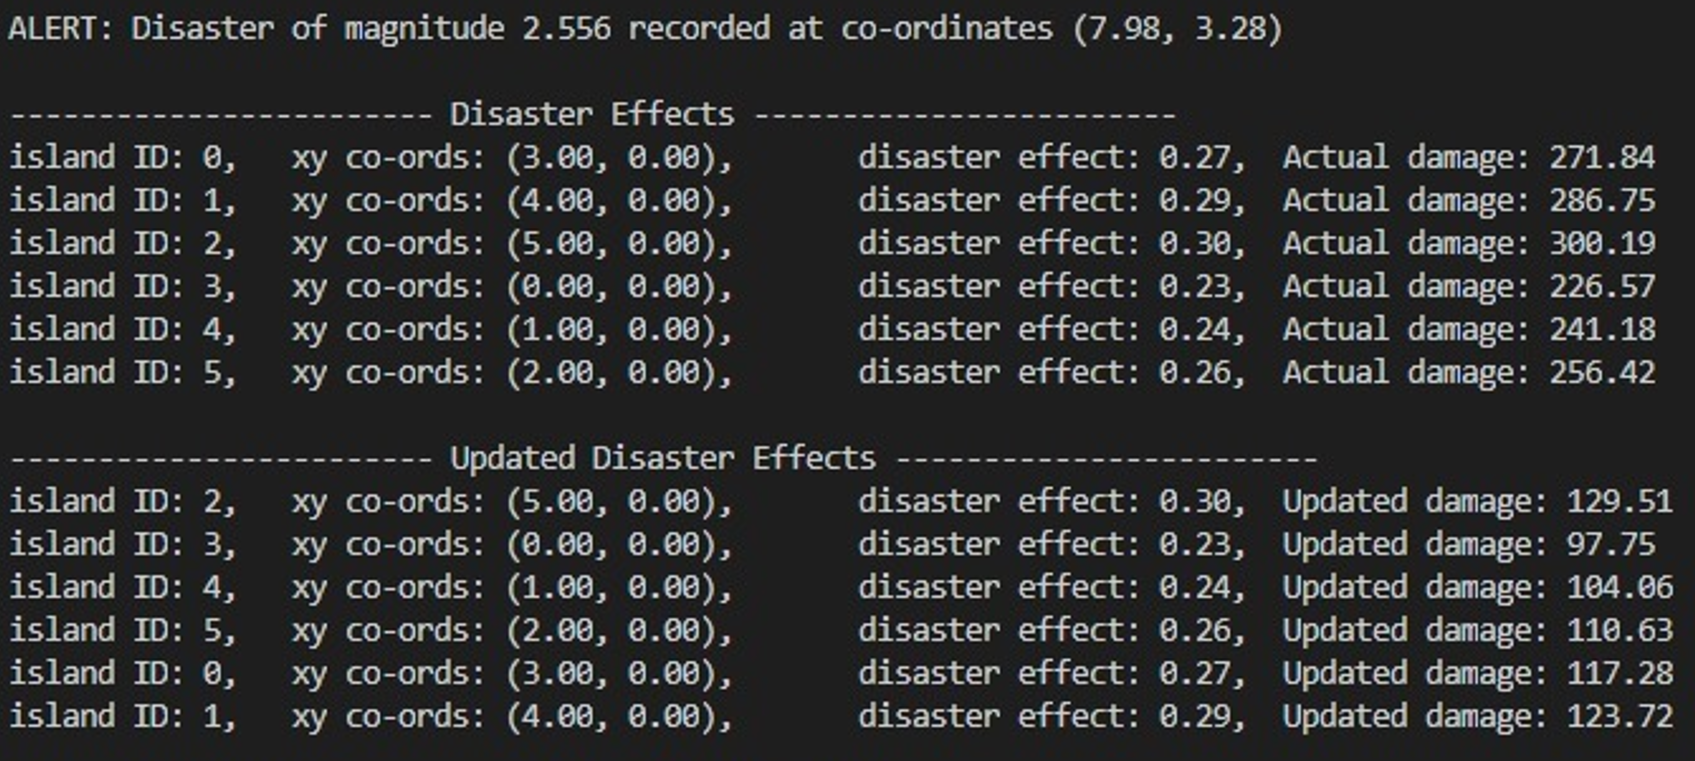
\includegraphics[width=0.5\textwidth]{04_environment/images/Common Pool infrastructure outcome.PNG}
    \caption{Demonstration of how common pool works in software}
    \label{fig:Common Pool infrastructure outcome}
\end{figure}


    \chapter{Inter-Island Trade Organisation (IITO)}

\section{Design}
\label{sec:IITO:Design}

The role of IITO is to facilitate inter-island communication and to enable the acts of giving and receiving gifts. In a more complete and realistic multi-agent simulation, unrestricted communication between the islands could have been considered, where islands could communicate with one another in an unconstrained manner. However, such a communication style would also assume the fact that the islands are rather complex agents which are able to undertake considerably sophisticated actions. Therefore, for the coursework, specific forms of communication were chosen to sensibly restrict the island complexity while still allowing for interesting interactions between the islands to take place.

\subsection{Inter-Island Communication}  
\label{subsec:IITO:inter_island_communication}

Islands which can communicate separately from the main governing body level of interactions (i.e. IIGO) makes more complex island behaviour possible. It was intended to allow the islands to be able to:

\begin{itemize}
    \item Inform other islands of the amount they intend to donate to the common pool.
    \item Share voting history with other islands\footnote{\label{footnote:IITO:future_work}This is not implemented in the final system, left as future work.}.
    \item Share tax amount history with other islands$^{\ref{footnote:IITO:future_work}}$.
    \item Inform other islands of the amount of resources they currently have in their private pool$^{\ref{footnote:IITO:future_work}}$.
\end{itemize}


\textbf{Common Pool Donations}: Allows islands to broadcast how much they plan to donate to the common pool and let them declare to the other islands if they plan to donate more than the specified tax amount put forward by the President as a form of virtue signalling. This may help an island redeem itself if it had previously lost trust. Note that an island can lie about the amount it will donate to the common pool if it is trying to maliciously gain favour. A further explanation of this part can be found in section \ref{subsec:IITO:intended_contribution}

\textbf{Voting History$^{\ref{footnote:IITO:future_work}}$}: Islands can request voting history from other islands or provide their own one unprompted. This interaction enables islands to verify whether the Speaker has been honest when counting the votes for a previously held election. Note that the islands can lie in the voting history that they provide, meaning that the islands may want to only take heed of information from those islands that they already trust.

\textbf{Tax History$^{\ref{footnote:IITO:future_work}}$}: Similarly to providing and requesting voting history, islands can request taxation history (i.e. how much the islands were told to contribute in the form of tax by the President) from other islands. Note that an island may choose not to provide this tax history, or it can be dishonest about it. If the islands report the true level of taxation, this interaction allows islands to form an opinion about whether the President has decided on a fair\footnote{Note that this fairness metric will be unique to each island, meaning that it is subjective.} amount of taxation.

\textbf{Current Resources$^{\ref{footnote:IITO:future_work}}$}: Islands are also able to share the value of the resources that they currently have in their private pool. This information may guide islands when making decisions regarding gifts (Section~\ref{subsec:IITO:gifting}). For example, if an island requests a gift because they are low on resources, the island receiving the request may want to ask how many resources the requesting island has. This can also give an island an indication of the overall level of richness in the archipelago. Similarly to sharing the intended common pool donations along with voting and tax history, the islands can decide not to report or lie about their current amount of resources.

\subsection{Future Work}
\label{subsec:IITO:futurework}
The full extent of what was discussed for the IITO was not implemented in the end. One of the main reason for this decision was to accommodate the need for a significant amount of time for improving the complexity of the agents (i.e. the islands) in the archipelago. Complexity in this case, meaning exploring deeper the features already present rather than introducing more. Therefore, some inter-island communication methods listed in section \ref{subsec:IITO:inter_island_communication} are left as future work. It is left as an exercise for the imagination of the reader to infer how such additional features would have been exploited by the islands in the archipelago. Team formation for foraging was also discussed, but ultimately abandoned
\subsubsection{Team formation}
This was intended as mechanic for allowing teams to explicitly forage together, in one way or another. One idea on how to implement this was to give members of already established teams the ability to accept or reject new members, and the main idea was that the islands would then decide on a foraging method and perform the action together, allowing for more explicit and formal communication. This was abandoned partially because the collaboration dilemma is already present in the current foraging design, so adding this added layer of formality and structure seemed to mostly just increase the complexity, without adding any new dilemmas. Even so, it would have been interesting to see if these explicit teams would have introduced more long-term strategies for foraging leading, and how it would have affected trust.

\subsection{Gifting}  
\label{subsec:IITO:gifting}  

If an island is struggling and requires some additional amount of resources to survive, it may ask the President for an allocation from the common pool but the President may reject this request. The struggling island would still be able to take resources from the common pool if rejected, but law-abiding islands would probably want to avoid such disobedience. To allow islands to still request an additional amount of resources from the other islands, the \textbf{gifting} action is an option. Islands may accept the gift requests if they wish to improve their standing with the requesting islands. They can also accept the gift requests of those whose survival is deemed to be essential for the future of the archipelago. When requesting, giving or receiving a gift, the island can specify a reason for this action, which gives islands more information about the gifting transaction. For example, a requesting island may want to specify that they will move to a critical state in the next round if they do not receive the gift, or an offering island may want to specify that the gift is meant as a reward for successful disaster forecasting.

Islands are also able to offer gifts without a request being made, meaning they can reach out to other islands if they want to boost their popularity.

\subsection{Intended contribution}
\label{subsec:IITO:intended_contribution}
When contributing to the common pool it would be great know how much other islands were planning on giving as well and thus be able to coordinate how much archipelago, as a whole, is actually planning on giving. A pattern similar to gifting could have established to encourage more explicit communication and discussion this contribution but in consideration for the other teams and to keep complexity low, the intended contribution was, instead, simply broadcast in the same way as in IIFO. Islands have the option to say how much they intend to contribute and to which islands they want to share this information and islands then receive the signaling information from the islands that explicitly shared their information with them. There is no further discussion past this point, so there is no good way of signaling a change of tactic based on the new information. It still has merit however, as it allows islands to build a history of how much other islands contribute to the main pool, assuming that the information sent is truthful obviously.
\section{Implementation}
\label{sec:IITO:Implementation}

\subsection{Server Client Infrastructure}
\label{subsec:IITO:server_client_infrastructure}  

During a turn, once IITO has started, a series of sessions are run, and the conclusion of all these sessions indicates that the IITO is also complete. In the current implementation, these sessions include gift giving and common pool donations, and they all follow the same client-server interaction format\footnote{Server and Client are defined in Definition~\ref{def:server} and Definition~\ref{def:client} respectively}. The server acts an intermediary for all client to client communication, and prompts clients to make decisions or formulate messages during the session. In IITO there are two sessions ran in sequence, gifting (section \ref{subsec:IITO:gifting_session}) and intended contribution signaling (section \ref{subsec:IITO:intended_contribution_session}). Together they facilitate trust based interaction and cooperation. 

\subsection{Gifting Session}
\label{subsec:IITO:gifting_session} 

There are four phases to the gifting sessions: Gift requests, gift offers, gift responses and updating gift history. Each part is further explained below and Figure~\ref{fig:IITO:gifting_session_diagram} shows the interactions a single client will have with the server over the session.
\begin{itemize}
    \item \textbf{Gift Requests}: This part collects the gift requests of all clients. These requests include an amount the client wants and who they wish to request from.
    \item \textbf{Gift Offers}: Here we give the clients any requests that are directed to them and then collects the gift offers from each client. These offers include an amount the client wished to gift and to whom the gift is being offered.
    \item \textbf{Gift Responses}: Here we provide the client with all the offers directed towards them and prompts them to respond to each of these offers. These responses contain the amount the client wishes to accept and a reason for their decision.
    \item \textbf{Updating Gift History}: In this stage client's are told of the outcome of any offers they gave out. A client is told whether or not an offer has been accepted, the reason for the rejection or acceptance and also the amount the receiver wishes take. For example Team 1 may offer $100$ resources to Team 2, but Team 2 may only want take $50$. The implemented system allows for such behaviour.
\end{itemize}

\begin{figure}[!htb]
    \centering
    \includegraphics[width=0.4\textwidth]{06_iito/images/gifting_diagram.png}
    \caption{Overview of client-server interactions in gifting session.}
    \label{fig:IITO:gifting_session_diagram}
\end{figure}

\subsection{Intended Contribution Session}
\label{subsec:IITO:intended_contribution_session}
The are only two steps to the Intended Contribution Session: The server side implementation is identical to the structure described in \ref{sec:IIFO:implementation}
\begin{itemize}
    \item \textbf{Share Intended Contribution Info}: This part collects the intended contribution information from all clients. This information includes the amount the client intends to contribute to the common pool and who they wish to share this information with.
    \item \textbf{Receive Intended Contribution Info}: In this stage the clients receive the other clients' contribution intentions. A client only receives these intentions from clients who explicitly said they wanted to share their intention with them.
\end{itemize}
The information passed has the only one single number representing how much the agent intends to contribute to the common pool. 
\begin{verbatim}
struct IntendedContribitionInformation = {
   IntendedContribution = Resources
}
\end{verbatim}
 % yeah, wrong numbering; I KNOW [Ezgi]
    \chapter{Inter Island Forecasting Organisation (IIFO)}

\section{Design}
The role of IIFO is to allow islands to make predictions about the likelihood and severity of disasters, and the amount of returns from foraging. The former is related to the long term collective risk dilemma (ltCRD), and the latter is related to the short term risk dilemma (stCRD).
\subsection{Long Term Collective Risk Dilemma (ltCRD)}
\label{subsec:IIFO:ltCRD}

Islands may build a model to try and predict the likelihood and severity of upcoming disasters. If desired, the islands are then able to share their predictions with other islands along with a confidence level for their predictions. This confidence level allows islands to signal how much confidence they have in their own prediction. Accordingly, in the case where the island's prediction turns out to be wrong, the other islands might not condemn them as harshly if the island's confidence level was indeed low. On the other hand, a higher confidence level indicates that other islands should potentially place more trust in this prediction with the risk that the island offering the information will be condemned more harshly if the prediction turns out to be wrong.

The motivation behind sharing these predictions is that with more islands contributing to the common pool, the effects of the disaster(s) can be more heavily mitigated. Therefore, sharing predictions allows islands to manage their resources in a more informed way, as they have a better idea of when and how much they should donate to the common pool in order to mitigate a future disaster.

Inaccurate predictions may result in a situation where the islands are not at all prepared for the incoming disaster. An example of this is to predict an incoming disaster belatedly, meaning that the common pool may not yet be sufficient enough to mitigate the disaster effectively when it hits the archipelago. Alternatively, the islands may also overprepare and donate too much to the common pool when, in fact, a disaster is not imminent, meaning they have unnecessarily reduced their own resources, making it harder for them to forage and build up resources again.
\subsection{Short Term Collective Risk Dilemma (stCRD)}
\label{subsec:IIFO:stCRD}

Predicting the returns from foraging in different locations is beneficial to the islands as it allows them to potentially maximise the returns if such predictions turn out to be accurate. IIFO enables the communication of these predictions between islands.

The benefit of sharing these predictions about foraging returns is due to the fact that foraging is typically performed by a group of islands. The more resources the islands put in, the greater the returns they are more likely to receive for each amount of input resource. This means that if an island is relatively confident about where the best returns can be found for foraging, it is in its interest to let other islands know in the hope that they will also decide to forage with them.

If the prediction proves to be inaccurate, the returns from foraging will be less than expected, and the islands that joined the foraging may lose faith in the future predictions of the island that originally proposed the inaccurate prediction. This may make it harder for the island whose predictions turn out to be wrong to convince others to forage together in the future.
\subsection{Future work}
As in IITO \ref{subsec:IITO:futurework} there were alot of features in IIFO which were discussed but did not make in to the final project. The same justification applies in this section as in IITO for why they were not implemented. There are a couple of features however that would have assisted current dilemmas by allowing agents to deliberate over them.
\subsubsection{Deer Population Sustainability}
With the deer population dropping as a result of foraging there are points of optimality in this dilemma where the deer population is not overhunted and maintains a stable population giving the islands high output. For this to be properly exploited the islands would need to have some sense of how many deer are in the population or the average output. A forum for discussing this or a new mechanic like scouting or population mapping would allow for exploring sustainable and responsible foraging.
\section{Implementation}
\label{sec:IIFO:implementation}
Disaster predictions (\ref{subsec:IIFO:disaster_pred}), foraging results (\ref{subsec:IIFO:foraging_history}) and common pool contribution intentions (\ref{subsec:IITO:intended_contribution_session})  are all shared through the same pattern described in figure \ref{fig:IIFO:information_share_infra}. To allow agents to choose freely who to communicate to the server asks the clients the following information:
\begin{verbatim}
struct Information = {
   Information = the information they want to send
   ShareTo = list of islands they want to share the information with
}
\end{verbatim}
The server then figures out what information goes to which agent and keeps track of which agent it was shared from and sends this information back out to the agents in the following format:
\begin{verbatim}
dictionary Information = {
   SharedFrom: Information
}
\end{verbatim}
\begin{figure}[!htb]
    \centering
    \includegraphics[width=0.35\linewidth]{07_iifo/images/Information_share_graph.png}
    \caption{IIFO and intended contribution information sharing}
    \label{fig:IIFO:information_share_infra}
\end{figure}
\subsection{Disaster Prediction}
\label{subsec:IIFO:disaster_pred}
Each round all agents are asked to share their predictions for when the next disaster happens. Disaster predictions, foraging history and common pool contribution intentions are all discussed in the same format described in \ref{sec:IIFO:implementation}. The information passed allows agents to share information about when they think the next disaster will happen, where it will strike, how strong it will be and how confident they are in their own prediction. The information passed has the format: 
\begin{verbatim}
struct DisasterPredictionInformation = {
   Magnitude = number,
   X,Y = coordinates,
   TimeToPrediction = turns,
   Confidence= percentage
}
\end{verbatim}

\subsection{Foraging History}
\label{subsec:IIFO:foraging_history}
Foraging returns depend on other island's contribution and foraging decisions. It is therefore important to know how much other islands spent on foraging, what resource they foraged and how much they got in return. This information allows agents to update their strategies in accordance to the other client's foraging tactics. The information: below is passed using the pattern described in \ref{sec:IIFO:implementation}
\begin{verbatim}
struct ForagingReturnsInformation = {
   ForagingReturn = resources,
   ForageType = deer or fishing,
   ResourcesSpentOnForaging = resources,
}
\end{verbatim}


    \chapter{Inter-Island Governmental Organisation (IIGO)}


The role of IIGO is to maintain, update, and revise the rules concerning provision to managing the long-term collective risk dilemma (ltCRD).

\begin{itemize}
    \item There will be 3 distinct branches in the IIGO: the \textbf{legislative branch}, \textbf{executive branch} and \textbf{judicial branch}\footnote{This is, as no surprise, inspired by the separation of powers in Western democracies.}.
    \item Each role is put in power according to the  transfer-of-power rules (see Section~\ref{subsec:transfer-of-power} for more detail).
    \item The head of the legislative branch is the Speaker, the head of the executive branch is the President, and the head of judicial branch is the Judge.
    \begin{itemize}
        \item  The Speaker, President and Judge are selected, through a democratic election, from the islands in the archipelago\footnote{This naming is inspired by the roles in the US Government.}.
        \item The resources gathered by the archipelago are endogenous, hence acting on the institutional powers granted to the Speaker, President or Judge costs resources.
        \item For their duty, the President, the Speaker and the Judge receive a salary for each of their turns in office (see Section~\ref{subsec:salary} for more detail).
        \item The limit of the powers of the President, Speaker and Judge are defined in this chapter (e.g. the Speaker can only call one vote per turn).

    \end{itemize}
\end{itemize}

\subsection{IIGO Specific Definitions}
\begin{definition} \label{def:ballot}
    A \textbf{ballot} is related to each island's \textbf{power} to support or disagree with the rule specified in the vote called by the President and to vote in favour or against an island for a specific role (i.e. the President, Speaker, Judge) at each round of the game.
\end{definition}


%\begin{definition} \label{def:vote}
    %A \textbf{vote} is related to a role's (i.e. the President, Speaker, Judge) \textbf{power} to call a vote for a specific rule or an election.
%\end{definition}


\begin{definition} \label{def:tax}
    The \textbf{taxation} is related to the President's \textbf{power} to request a specific \underline{\textbf{minimum}} amount of contribution from each island to the common pool at each round of the game.
\end{definition}

\begin{definition} \label{def:alloc_req}
    An \textbf{allocation request} is related to each island's \textbf{power} to request a specific amount of resource allocation from the President at each round of the game.
\end{definition}


\begin{definition} \label{def:rule_prop_list}
A \textbf{rule proposal list} is related to each island's \textbf{power} to propose a specific rule to be passed to the President at each round of the game.
\end{definition}

\begin{definition} \label{def:invst}
    An \textbf{investigation} is related to the Judge's \textbf{power} to acquire information to make a decision, followed by a calculation of the expected results and checking whether some specific rules have been obeyed, exclusively for the actions carried out by the \textbf{islands}.
\end{definition}


An example of an \emph{investigation}: The President has permitted the island $X$ to take the amount of $Y$ resources from the common pool. Upon \emph{investigation} carried out by the Judge, it is revealed that the amount of resources taken out from the common pool by the island $X$ is, in fact, $Y'$ such that $Y' \neq Y$.


\begin{definition}
\textbf{Monitoring} is a government official's \textbf{power} to perform event recognition and to check whether some specific rules have been obeyed.
\end{definition}

An example of \emph{monitoring}: The Speaker has performed only the following action: \emph{counted the votes and calculated the result} for a rule. Upon \emph{monitoring} carried out by the President, it is noticed that the Speaker has not made any \emph{announcement}. Hence, the Speaker has not followed their obligation to \emph{announce} the result of any vote held.

See Section~\ref{sec:accountability} for more information about which roles can monitor which ones.


\begin{definition}
\textbf{Investigative-monitoring} is a government official's \textbf{power} to acquire the information used in acting on a governmental power followed by calculation of the expected results and checking whether some specific rules have been obeyed, exclusively for the actions carried out by a government official they are responsible for.
\end{definition}

An example of \emph{investigative-monitoring}: The Speaker has performed the following actions: \emph{counted the votes and calculated the result $R$} for a vote $V$ and \emph{announced} the result $R'$ for the vote $V$. Upon \emph{investigative-monitoring} carried out by the President, it is noticed that $R' \neq R$. Hence, the Speaker has modified the announced result.


\begin{definition}
The \textbf{sanction} is related to the Judge's \emph{power} to punish non-compliant islands when their disobedience is confirmed through investigations at a specific turn.
\end{definition}


\begin{definition}
The (judicial) \textbf{pardon} is related to the Judge's \emph{power} to forgive a non-compliant island at a specific turn.
\end{definition}

\begin{definition}
The \textbf{budget} is the maximum amount of resources a role is permitted to spend from the common pool as it performs its own institutional-power-enabled actions at a specific turn.
\end{definition}


\begin{definition}
The \textbf{salary} is the amount of resources a role is to be given from the common pool as a reward for performing its institutional-power-enabled actions at a specific turn.
\end{definition}

\begin{definition} \label{def:term}
A \textbf{term} is the number of turns an island is \emph{permitted} to hold a role, and after which the responsible role (indicated in the transfer-of-power cycle in Figure~\ref{fig:cycles_in_IIGO}) is \emph{obliged} to initiate transfer-of-power.
\end{definition}

\subsection{\emph{Power}, \emph{Permission} and \emph{Obligation} Distinction}
In the rest of the specifications, we will be specifically using the following three terms to define the actions and responsibilities carried out by the Speaker, President, Judge (see Figure~\ref{fig:per_obl_sets}):
\begin{itemize}
    \item Power
    \item Permission
    \item Obligation
\end{itemize}



\begin{figure}[H]
\centering
\includegraphics[width=0.6\textwidth]{05_iigo/images/SOMAS_per_obl.pdf}
\caption{Relationship between \emph{power}, \emph{permission} and \emph{obligation}.}
\label{fig:per_obl_sets}
\end{figure}


For example, the Judge has the \emph{power} to carry out investigations at an IIGO session. There are no rules specifying which specific islands the Judge should investigate. Therefore, the Judge has the \emph{permission} to investigate any `alive' islands during a session. However, the Judge is \emph{obliged} to make at least some number of investigations each turn.



\section{Executive Branch}
\label{sec:executive}
The executive branch is responsible for \textbf{carrying out the law}.
\begin{itemize}

    \item The President has the \emph{power} to:
    \begin{itemize}

        \item Select a rule for voting $R^{*}$ to be passed to the Speaker.
        \begin{rule_IIGO}
            The President has the \emph{obligation} to \emph{select} a rule $R^{*}$ if the \emph{rule proposal list} has at least one proposed rule in it.
        \end{rule_IIGO}
        \begin{rule_IIGO}
            The President has the \emph{permission} to \emph{select} a rule $R^{*}$ if and only if $R^{*} \in S$, where $S$ is the \emph{rule proposal list}.
        \end{rule_IIGO}

        \item Decide the amount of individual \emph{taxation} (i.e. a specific \emph{minimum} amount of contribution to the common pool for each island) for the current turn.

        \begin{itemize}
            \item The President is given the self-reported resource amounts held by each island to assist in this decision.
            %\item Suggested Rule: For any island that has chosen to not report it's resources, the President has the \emph{obligation} to set them an individual tax amount T.
        \end{itemize}

        \item Decide the allocation of resources distributed from the common pool to the islands (i.e. a specific \emph{maximum} amount an island is permitted to take from the common pool).

        \begin{itemize}
            \item The President is given the \emph{allocation requests} made by each island.
            %\item \emph{}{Suggested Rule:} The President has an obligation to prioritise islands in critical condition.
        \end{itemize}
    \end{itemize}
\end{itemize}



\section{Legislative Branch}
\label{sec:legislative}
The legislative branch is responsible for \textbf{making the law}.
\begin{itemize}

    \item The Speaker has the \emph{power} to:
    \begin{itemize}

        \item Call a vote $V$ for a rule $R$.
        \begin{rule_IIGO}\label{rule:call_vote_obl}
            The Speaker has an \emph{obligation} and a \emph{permission} to \emph{call} a vote $V$ if and only if the President has \emph{selected} a rule $R$ to be voted on.
        \end {rule_IIGO}
        \begin{rule_IIGO} \label{rule:call_vote_perm}
            The Speaker has the \emph{permission} to \emph{call} a vote $V$ for a rule $R$ if and only if the rule $R = R^{*}$, where $R^{*}$ is the rule \emph{selected} by the President.
        \end {rule_IIGO}

        \item Choose which islands are participating in the vote $V$.
       % \footnote{This is our sequential implementation alternative for the power to close the ballot box.}.
        \begin{rule_IIGO} \label{rule:all_islands_vote}
            The Speaker has the \emph{obligation} to ask for a vote from all alive islands.
        \end {rule_IIGO}

        \item Declare the result $C$ of a vote $V$.
        \begin{rule_IIGO}
            The Speaker has an \emph{obligation} and a \emph{permission} to \emph{declare the result} $C$ for a vote $V$ if and only if the vote V has been \emph{called}.
        \end {rule_IIGO}
        \begin{rule_IIGO}
            The Speaker has the \emph{permission} to \emph{declare the result} $C$ for a vote $V$ if $C = C^{*}$, where $C^{*}$ is the result produced by \emph{calling} the vote $V$.
        \end {rule_IIGO}
        \begin{itemize}
            \item This step is what enables a rule to be \emph{active}.
        \end{itemize}
    \end{itemize}
\end{itemize}




\section{Judicial Branch}
\label{sec:judicial}

The judicial branch is responsible for \textbf{evaluating the law}.
\begin{itemize}
    \item The Judge has the \emph{power} to:
    \begin{itemize}
        \item Perform a number of \emph{inspections}\footnote{An \emph{inspection} \textbf{costs} an expense of resources (See Definition~\ref{def:invst} for more detail).} $I$ and produce a compliance outcome $\mathbb{O}^{*}$\footnote{Note that the compliance outcome $\mathbb{O}^{*}$ considered is a boolean.}.
        %(true: the island has been compliant with the rules in play, false: the island has not been compliant with the rules in play)
        %\begin{itemize}
           % \item For example, to check if the event outcome is \emph{concurrent}\footnote{Again, what is defined as "concurrent"? A clear definition is needed.} with the rules.
        %\end{itemize}
        \begin{rule_IIGO}
            The Judge has the \emph{obligation} to make at least $N$ investigations at each turn.
        \end{rule_IIGO}
        \item Declare the outcome $\mathbb{O}$ of an inspection $I$ to all islands\footnote{This act of broadcasting is especially important for islands to form an opinion about the sanctioned islands accordingly.}.
        \begin{rule_IIGO}
            The Judge has an \emph{obligation} and a \emph{permission} to declare the outcome $\mathbb{O}$ of an inspection $I$ if and only if the inspection $I$ has been performed.
        \end{rule_IIGO}
        \begin{rule_IIGO}
            The Judge has the \emph{permission} to declare the outcome $\mathbb{O}$ of an inspection $I$ if $\mathbb{O} = \mathbb{O}^{*}$, where $\mathbb{O}^{*}$ is the outcome of the inspection $I$.
        \end{rule_IIGO}
        %\item Initiate the removal of the \texttt{President}.
        %\begin{itemize}
            %\item A good Judge would be especially vigilant during \emph{power transfer} regarding the \emph{President} position (see Section~\ref{leg_const} for more detail).
        %\end{itemize}
        \item Invoke economic \textbf{sanctions} (see Section~\ref{sec:sanctions} for more detail).
        \begin{rule_IIGO}
            The Judge has an \emph{obligation} and a \emph{permission} to invoke a sanction $S$ for an island $X$ if and only if an investigation $I$ has an outcome $\mathbb{O}^{*}$ indicating non-compliance, and $I$ is an investigation of an action taken by island $X$.
        \end{rule_IIGO}
        \item Invoke even more severe sanctions in the case of further disobedience to previous sanction(s).
        \begin{rule_IIGO}
            The Judge has the \emph{permission} to invoke a severer sanction $S'$ for an island $X$ if the island $X$ has not fulfilled the requirements of the previous sanction $S$.
        \end{rule_IIGO}
        \item Pardon the islands which are currently sanctioned.
        \begin{rule_IIGO}
            The Judge has the \emph{permission} to revoke any sanction $S$ of an island $X$ at a specific turn.
        \end{rule_IIGO}
    \end{itemize}
\end{itemize}
%(e.g. a new rule that falls under a "sanction" category \hl{[I'm not sure about this being a `new rule` [Ezgi]]}

\subsection{Sanctions}
\label{sec:sanctions}
All sanctions are of economic nature which include:
        \begin{itemize}
            %\item Revoking an island's access to the common pool.
            \item Enforcing an island to contribute a specific amount of resources to the common pool.
            \begin{itemize}
                \item This does not mean that the Judge has the \emph{power} to take resources from an island in order to put them to the common pool -- the island itself is expected to carry out this implication imposed by the sanction itself, otherwise further punishment can be induced by the Judge.
                \item Similarly, \emph{opinion formulation} will follow accordingly whether the island(s) is/are following the implications imposed by the sanction(s).
            \end{itemize}

    \end{itemize}
    Sanctions are the associated penalty that comes with an island breaking a specific rule. The Judge is in full control of the penalties associated with breaking any rules. Once the Judge has specified the score of the penalty associated with each time an island breaks a rule, the cumulative penalties accumulated by the island are then used to determine which \textbf{sanction tier} that each island falls into. The score threshold to determine the boundaries of the sanction tiers are set by the Judge. At each turn of the game, each island is told whether they are being sanctioned, and if so, which \textbf{sanction tier} that they are currently in. The \textbf{sanction tiers} of the non-compliant islands are also broadcasted to the other islands in the archipelago. To summarize, the sanctioning process follows these steps:



    %Sanctions are based on an island breaking a rule. Each rule must therefore have an associated penalty. By default, we set these penalties such that they add $1$ to the total sanction score for each island. However, we allow the judge to override this scoring, the judge is able to set their own scores for any particular rule as they desire. This custom scoring is then used when an island breaks a particular rule. By looking at events that occurred in the last turn, and using the customised scoring we provide the holder of the judge role with full control of the penalties for breaking any rules.







%we then use the cumulative penalties accumulated by each island to determine which Sanction Tier they fall into. The score threshold's required to fall into these sanction tiers is set by the judge and is checked for monotonicity. Each island is told whether they are being sanctioned, and is so what tier they are in. We also tell other islands about which sanction tiers other islands have fallen into.

    \begin{enumerate}
        \item The Judge has the \emph{power} to set custom penalties associated with breaking any rules.
        \item The Judge is given a list of all events that occurred in the previous turn.
        \item The Judge has the \emph{power} to check whether any, or all of these previous events, involve the islands in the archipelago breaking any rules.
        \item Each of the transgressions is scored using the Judge's custom penalties if the Judge has set them. Otherwise, a score of $1$ is given each time a rule is broken.
        \item The Judge has the \emph{power} to revise the sanction thresholds.
        \item Using the latest sanction thresholds available, each island is assigned to a sanction tier based on the sanction score that it has received.
        \item These sanction tiers are broadcasted to all of the islands in the archipelago.
        \item The Judge then uses sanctions rules in place to calculate the specific amount of resources that each non-compliant island has in order to determine how much it should contribute to the common pool, based on the sanction tier that it is in.
    \end{enumerate}



\section{Constitutional Rights and Obligations in the Archipelago}
\label{sec:const_rights_obl_archi}
Each island has the \emph{power} to:
\begin{itemize}
\item make an \emph{allocation request} (see Definition~\ref{def:alloc_req}) to the President for a specific amount to be allocated to them.
\item report the number of resources it is in possession of to the President.
\begin{rule_IIGO}
    Each island has the \emph{obligation} to report the number of resources it is in possession of to the President.
\end{rule_IIGO}
\begin{rule_IIGO}
    Each island has the \emph{permission} to report the number of resources $R'$ if and only if $R' = R$, where R is the number of resources the island is in possession of.
\end{rule_IIGO}
\item take resources from the common pool.


\begin{rule_IIGO}
    Each island has the \emph{permission} to take at maximum $N$ resources, where $N$ is the specific allocation made by the President to that island\footnote{If no such allocation is made, the island is \emph{permitted} to take any amount of resources.}.
\end{rule_IIGO}
\item contribute resources to the common pool.
\begin{rule_IIGO}
    Each island has the \emph{obligation} to contribute to the common pool an amount greater or equal to that of the individual tax set by the President.
\end{rule_IIGO}
                %The President is in
                %(unless there is a rule in place that dictates how Speaker is to allocate resources).
\item add a rule to the \emph{rule proposal list} (see Definition~\ref{def:rule_prop_list}) at the start of each turn.
        %\begin{itemize}
            %\item The game specification includes how many rules an island can propose each turn.
        %\end{itemize}
        %\item vote  for rules in the Legislative Branch and vote for their favourite islands in elections
\item participate in the legislative branch of the government by casting ballots in votes called by the Speaker.
\item vote for an island to be elected for a specific role (e.g. the President, Judge, Speaker) during the elections\footnote{This will be assumed to be true \underline{unless stated otherwise}. %Note that \textbf{diplomatic sanctions} can disable this power of a specific island (see Section~\ref{jud_const}).}.
        }.
\end{itemize}
\section{Accountability Cycle}
\label{sec:accountability}

The IIGO roles (i.e. the President, Speaker and Judge) hold a considerable amount of \emph{power}. To ensure that the government is able to avoid corruption and abuse of power, each branch of IIGO is accountable to another through the accountability cycle. 
The President is accountable to the Speaker, the Speaker is accountable to the Judge, and the Judge is accountable to the President (see Figure~\ref{fig:cycles_in_IIGO}). This accountability cycle is enacted through \emph{monitoring} actions\footnote{Note that the terms \textbf{monitoring} and \textbf{investigation} have similar but not identical meanings and different consequences in the context of IIGO.}. The desired effect is for any wrong-doing in IIGO to be determined as quickly as possible and the role in question to be replaced. 

The powers related to the accountability cycle and transfer-of-power for each role can be summarized as the following: 

\begin{itemize}
    \item The Speaker has the \emph{power} to:
    \begin{itemize}
        \item monitor the President.
        \item declare the result of this monitoring and and if the monitoring result indicates wrongdoing, oblige the Judge to initiate power transfer for the President.
    \end{itemize}
    \item The President has the \emph{power} to:
    \begin{itemize}
        \item monitor the Judge.
        \item declare the result of this monitoring and if the monitoring result indicates wrongdoing, oblige the Speaker to initiate power transfer for the Judge.
    \end{itemize}
    \item The Judge has the \emph{power} to:
    \begin{itemize}
        \item  monitor the Speaker.
        \item declare the result of this monitoring and and if the monitoring result indicates wrongdoing, oblige the President to initiate power transfer for the Speaker.
    \end{itemize}
\end{itemize}

%Unlike investigations performed by the Judge, who performs investigations on island actions in the following turn, each role is given the opportunity to check up on the actions of the role it is responsible for immediately after they have been performed. In this sense, the President can monitor (includes investigative-monitoring) the powers (calling a vote and announcing the result) acted on by the Speaker immediately after the Speaker's announcement (or lack there of). The government officials hold a lot of power so this is to ensure that any wrong-doing is determined as quickly as possible. For this project we are only pursuing one degree of monitoring, that is, the powers relating to the accountability cycle will not be monitored themselves. We assume that agents will act in the interest of themselves and keeping all the islands alive is beneficial to everyone. Hence, while the agents might be inclined to break rules in order to benefit themselves, anyone else breaking the rules is seen as undesirable under the assumption that the system in place is there to benefit all.

The result of monitoring is intended to be a trigger for the initiation of power transfer, whereby a declaration of a negative result indicates that at least one rule was broken by the role monitored and the role should be re-elected. Each turn, in addition to monitoring the actions taken by the role in that IIGO session, the election that role held in the previous IIGO session, if one was held at all, is checked for compliance with the rules of power-transfer.

Figure~\ref{fig:cycles_in_IIGO} illustrates the reverse nature of the monitoring and transfer-of-power cycles. This is a design choice made to diversify the islands that hold the powers that enable the process of a role's premature removal from power as a result of wrongdoing, hence helping to avoid malice. If it is one role's power to monitor, it is the other role's power to initiate and facilitate power transfer. Hence the latter is given a second opinion for cases where the declaration of wrongdoing is not truthful.

Within the scope of the coursework, we decided to pursue only \emph{one degree of monitoring}, meaning that the powers relating to the accountability cycle will not be monitored themselves. We assume that agents will act in the interest of all the islands in the archipelago. Hence, while the agents might be inclined to break the rules to benefit in some form, it is assumed that the others will negatively see any non-compliant islands based on the assumption that the proposed IIGO system is in place to maintain the welfare of all the islands. We still have rules governing this process (see Rule~\ref{rule:monitoring_1} and Rule~\ref{rule:monitoring_2}) although these rules are not enforced.


The \emph{one degree of monitoring} is another justification for the reverse nature of the monitoring and transfer-of-power cycles. The addition of a second opinion means that a role does not hold the power to both wrongfully declare wrongdoing and hold an election for the same role.

Let role $X$ be accountable to the role $Y$, which is accountable to the role $Z$. Then:
\begin{rule_IIGO} \label{rule:monitoring_1}
    $Y$ has an \emph{obligation} and a {permission} to declare the outcome of the monitoring result $M$ associated with the action $A$ undertaken by $X$ if and only if $Y$ has monitored the action $A$ performed by $X$.
\end{rule_IIGO}
\begin{rule_IIGO} \label{rule:monitoring_2}
    $Y$ has the \emph{permission} to declare the monitoring result $M$ associated with the action $A$ undertaken by $X$ if and only if $M = M^{*}$, where $M^{*}$ is the outcome of \emph{monitoring} action $A$ performed by $X$\footnote{These constitutional rules should be available to the agents to check their decisions against. However, due to having only one degree of accountability cycle in place, these rules are not enforced through any sanctions (i.e. breaking these rules has no consequence as they are only deemed to be an \emph{agreement} between the roles).}.
\end{rule_IIGO}


\begin{figure}[!htb]
\centering
\includegraphics[scale=0.33]{05_iigo/images/role cycles.png}
\caption{Accountability cycle (left), the transfer-of-power cycle (middle) and salary cycle (right).}
\label{fig:cycles_in_IIGO}
\end{figure}


\subsection{Transfer-of-power}
\label{subsec:transfer-of-power}

For the scope of this project, we chose elections to be the only system of power transfer for the islands to utilise. The islands that hold institutional power are the decision group of the archipelago. They decide on taxes, allocations and sanctions. By holding an election for the institutional roles, the islands are not directly included in the decision group, but they do participate in deciding who will occupy these roles and thus, who makes the aforementioned decisions. Elections also open up another avenue for opinion formation to have an effect.
\begin{itemize}
    \item Each role has the \emph{power} to call an election vote and declare the winner (see Figure~\ref{fig:cycles_in_IIGO} for the transfer-of-power cycle).
\end{itemize}

We note that:
\begin{enumerate}
    \item The Speaker conducts an election to appoint a new Judge.
    \item The Judge conducts an election to appoint a new President.
    \item The President conducts an election to appoint a new Speaker.
\end{enumerate}
Refer to the Figure~\ref{fig:cycles_in_IIGO} for further clarification about the transfer-of-power cycle.

We introduce a \emph{term} length to increase the diversity of the decision group. If the Rule~\ref{rule:roles_must_hold_election} is in play, the roles are obliged to hold an election every $N$ turns. To reduce the scope of the coursework, the term length is defined as a configuration parameter. Thus, we reduce the complexity of rules surrounding the election of roles and hence the reasoning the agents have to do with regard to these rules.

\begin{rule_IIGO} \label{rule:roles_must_hold_election}
    The role $X$ has an \emph{obligation} and a \emph{permission} to conduct a vote for the election of $Y$ if and only if $Y$ has been in power for more turns than the turn length or if role $Z$ has made a monitoring announcement that indicates wrongdoing by $Y$.
\end{rule_IIGO}

\begin{rule_IIGO} \label{rule:must_appoint_elected_island}
    The role $X$ has the \emph{permission} to \emph{declare the winner} $W$ for an election $E$ if $W = W^{*}$, where $W^{*}$ is the winner produced by \emph{calling} a vote for the election $E$.
\end {rule_IIGO}

Unlike the rule vote held by the Speaker, the process of election is more regimented. The power of calling a vote for an election and the power of declaring the result are combined into one action. This decision came as a result of a motion to simplify the system for implementation. However, the powers are still kept somewhat separate. When facilitating an election, the roles still have the option to declare a winner of their choosing. Rule~\ref{rule:must_appoint_elected_island} is what governs this choice. However, the agents do not have the option to not declare a result at all: holding an election will always result in a declaration of the winner.

\section{Budget and Salary}
\subsection{Budget}
%Actions associated with the IIGO have an associated cost that is defined as a configuration parameter. The institutional-power-enabled actions of  identified to require a "computational" component are:


For the simulation, we have defined the resources gathered by the islands to be endogenous. Hence we assume that self-organization will consume those resources and institutional-power-enabled actions in the IIGO have an associated cost. The institutional-power-enabled actions with such a cost are:



%that is defined as a configuration parameter. The institutional-power-enabled actions of  identified to require a "computational" component are:


%We have defined the resource to be an endogenous one, hence any computation surrounding the distribution of the resource must use up some of that resource.
\begin{itemize}
\item President selecting a rule from the rule proposal list.
\item President deciding the amount of taxation.
\item President deciding the allocation of resources from the common pool.
\item Speaker calling a vote and calculating the winner.
\item Judge inspecting an island's actions.
\item Judge inspecting an island's action history retrospectively.
\item Declaring (e.g. \textit{announcing} the result of a vote).
\item Holding an election.
\item Monitoring a role.
\end{itemize}

IIGO has been designed to act in the common good. Therefore IIGO-related costs will be directly withdrawn from the common pool. Since the common pool is considered communal property of the archipelago, there are rules in place to limit how much each role is allowed to spend in order to perform its own institutional-power-enabled actions. This is the reason for defining the \emph{budget} and keeping it separate for each of the three IIGO roles.

\begin{rule_IIGO} \label{rule:budget}
    %Each role has the \emph{obligation} to pay the salary of amount $S$ to another if and only if the amount paid $S'$ is equal to $S$.
    Each role has the \emph{permission} to act on an institutional-power-enabled action with an associated cost if the budget would not become negative as a result of performing the action.
 \end{rule_IIGO}



When a role acts on an institutional-power-enabled action with a cost, the cost associated with this action is subtracted from the role's \emph{budget}. If Rule~\ref{rule:budget} is in play, a budget of zero or less means that the role does not have the \emph{permission} to perform any of its institutional-power actions. The removal of Rule~\ref{rule:budget} from the rules in play means the role is permitted to perform as many such actions as it would like (as long as those actions are not governed by other rules).

The \emph{budget} is persistent across turns. This means that, assuming nothing else affects the budget, if a role has $100$ resources in its budget at the start of a turn and spends $10$ resources, the same role has $90$ resources in its budget at the start of next turn. On the other hand, islands can choose to increase the budget periodically at every turn. The islands can choose the magnitude of this periodic increase by voting on a rule.

%one turn and it spends 10, it has 90 resources in it's budget the next turn.



Finally, it must be noted that the budget is inherently linked with  whether the obligations of a specific role can be undertaken.
For example, during \emph{monitoring}, it is not seen to be a rule violation if a role has not acted on an obligation as doing so would require it to go over budget.

%This can also be seen as an added clause "... and the action is only permitted if they have the budget" to most rules which govern actions with an endogenous-cost.
%\begin{rule_IIGO}
    %The budget is increased by an amount $N$ every turn.
%\end{rule_IIGO}

%This rule means that, assuming nothing else affects the budget, if a budget is set to increase by 10 resources every turn and the budget is a 100 resources in turn one, the budget is 110 resources in turn 2. Setting this rule to 0 is equal to removing this rule and it means that the budget is never increased.


\subsection{Salary}
\label{subsec:salary}
A salary is paid to each role in power as an incentive to be in power. Since our system has regimented the means of power transfer to be an election, this incentive extends to acting in a publicly approved way. %Hence, each role has the \emph{power} to pay a salary to another role following the salary cycle in Figure~\ref{fig:cycles_in_IIGO}.
\begin{rule_IIGO} \label{rule:salary}
   Each role has the \emph{obligation} to pay the salary of amount $S$ to one another following the salary cycle in Figure~\ref{fig:cycles_in_IIGO}.
\end{rule_IIGO}

In Rule~\ref{rule:salary}, setting $S=0$ (through changing the active rules in place) means that roles do not have the permission to pay any salary. Removing the Rule~\ref{rule:salary} means that the roles may freely choose the amount $S$ for the salary payments.

\section{IIGO Session Order}
Each IIGO Session can be broken down into a sequence of consecutive actions by the Judiciary, Executive and Legislature. The session is concluded with monitoring, salary payments and elections.
\subsection{Judicial Actions}
\begin{enumerate}
    \item The Judge has the \emph{power} to check the history of actions to confirm whether the previously punished island(s) has/have obeyed the previous round's sanctions, meaning whether they contributed to the common pool accordingly in case of economic sanctions.
    %\begin{itemize}
      %  \item \emph{Suggested Rule:} In case of disobeying sanctions, the Judge is \emph{obliged} and \emph{permitted} to increase the severity of sanctions with respect to specific islands.
   % \end{itemize}
    \item The Judge has the \emph{power} to carry out \emph{inspections} on the history of actions of any island $X$ to check whether:
        \begin{enumerate}
        \item the reported resources of $X$ in the previous round match the real value of resources $X$ had in its private pool for the previous turn.
        \item the island $X$ has retrieved the right amount of the resources from the common pool, based on the \emph{allocation request} evaluated by the previous President.
            \begin{itemize}
            \item An example: In the previous round, the President has decided that the island $X$ can take $Y$ amount of resources from the common pool. If the Judge finds out that the island $X$ has taken an amount of $Y'$ such that $Y' > Y$, the Judge has the \emph{power} to invoke sanctions on the island $X$.

            %the Judge is \emph{obliged} and \emph{permitted} to sanction island $X$.
            \end{itemize}
        \end{enumerate}
    \item The Judge has the \emph{power} to invoke sanctions based on the outcome of the inspections.
\end{enumerate}
\subsection{Executive Actions}
\begin{enumerate}
    \item The islands may report the resources in their private pools to the President.
    \item The President has the \emph{power} to let each island know about the amount of \emph{taxation} they have to pay.
    \item The island has the \emph{power} to make an \emph{allocation request} to the President.
    \item The President has the \emph{power} decide on an allocation of resources and let each island know about the amount of resource allocation they are permitted to take from the common pool.
    \item The island has the \emph{power} to pick and to propose a rule to be voted on to the President.
    \item The President has the \emph{power} to choose a rule to be voted on from the received rule proposals.
\end{enumerate}
\subsection{Legislative Actions}
\begin{enumerate}
    \item The Speaker has the \emph{power} to call a vote.
        \begin{enumerate}
        \item The islands vote in support of, or against, the rule (aye or nay) anonymously.
        \end{enumerate}
    \item The Speaker has the \emph{power} to announce a result of a vote to the islands and carries out the law change, if required (e.g. deleting/rejecting a rule if there is a majority nay vote).
\end{enumerate}
\subsection{End of Session Actions}
\begin{enumerate}
    \item The roles pay a salary to one another following the accountability cycle in Figure~\ref{fig:cycles_in_IIGO}.

    \item The Speaker has the \emph{power} to decide to carry out \emph{monitoring} on:
    \begin{enumerate}
    \item the resource allocation decided by the President.
    \item the rule proposed by the President.
    \item the previous IIGO session's election for a new Speaker, if an election was held.
    \end{enumerate}
    \item The President has the \emph{power} to decide to carry out \emph{monitoring} on:
    \begin{enumerate}
        \item the sanctions imposed by the Judge.
        \item the previous IIGO session's election for a new President, if an election was held.
    \end{enumerate}
    \item The Judge has the \emph{power} to decide to carry out \emph{monitoring} on:
    \begin{enumerate}
        \item the vote called by the Speaker.
        \item the Speaker announcing the result.
        \item the previous IIGO session's election for a new Judge, if an election was held.
    \end{enumerate}
    \item The Speaker has the \emph{power} to decide to hold an election for a new Judge.
    \item The President has the \emph{power} to decide to hold an election for a new Speaker.
    \item The Judge has the \emph{power} to decide to hold an election for a new President.
\end{enumerate}

\section{Implementation} % INFRA implementation to be written here

\subsection{IIGO Branches Overview}
The IIGO branches have been implemented to facilitate the use of powers given to the IIGO Roles. Because any agent could potentially become the President, Speaker or Judge, the implementation of each of the corresponding branches has been split into two interconnected parts:

\begin{itemize}
\item Client-side implementation of President, Speaker and Judge functions, which map directly to the powers given to that role.
\item Server-side implementations of Executive, Legislative and Judicial branch actions, which call the IIGO role functions only on the client currently holding that role i.e. the executive branch only calls functions on the client assigned to the role of President.
\end{itemize}

\subsubsection{Client-side Overview}
The client-server division gives agents the freedom to implement the IIGO role functions as they like, provided that they follow the specified interface. Some agents may choose to obey the rules to ensure that the IIGO role inspecting their actions will never find any wrongdoing. When implementing their President, Speaker and Judge functions, islands can either follow a rule-obeying approach or try to exploit their power once they are elected to be an IIGO role. For example, the President gets access to the reported amounts of private pool resources from all the islands and therefore, can use this confidential information for its own benefit in foraging or gifting.

\subsubsection{Server-side Overview}
The server implementation of each branch provides the IIGO roles with the framework to use their powers of carrying out the law in the archipelago. The server is responsible for the vast majority of data processing and acts as a bridge between the IIGO roles and the other agents. For example, the President decides on the tax distribution for the given turn, and the server converts this information into communication messages and broadcasts them to the islands. This ensures that the backend 'logistics' of the game, such as the format of messages passed between islands, remain the same between different implementations of each IIGO role. It also reduces the complexity of agents and minimizes the amount of work for each of the team implementing their agents.

Moreover, the server acts as a guard of the game state and prevents the clients in IIGO roles from performing game-breaking actions. For example, server-side of the IIGO branches ensure that the roles are only allowed to consider taking any action only if the monetary constraints allow. In other words, if the amount of resources in the common pool is lower than the action cost, then the role is not allowed to perform this action, as it would result in a negative amount of resources in the common pool. However, if the common pool holds enough resources, then it is up to the island implementation to decide whether the role will act on its powers.


\subsection{Executive Branch}


\subsubsection{Client-side}

\label{sub:president:client-side}
Each agent can become the President at any turn. Therefore each agent should implement all of the presidential functions according to the common interface. Those functions directly correspond to the powers of the executive branch outlined in Section~\ref{sec:executive} as well as accountability and transfer-of-power obligations outlined in Section~\ref{sec:accountability}. 

The presidential functions can be divided into two categories:
\begin{enumerate}
\item Presidential power functions:
    \begin{itemize}
        \item \texttt{SetTaxationAmount} allows the President to decide the amount of taxation individually set to each island. Returns the $map[agent] \xrightarrow[]{} tax$, as well as information about whether the President has acted on its power to set taxation.
        \item \texttt{EvaluateAllocationRequests} allows the President to decide the allocation of resources distributed from the common pool to the islands. Returns the $map[agent] \xrightarrow[]{} allocation$, as well as information about whether the President has acted on its power to set allocation to common pool resources.
        \item \texttt{PickRuleToVote} allows the President to select a rule for voting $R\ast$ to be passed to the Speaker. Returns the $rule$ to be voted on by the Speaker, as well as information about whether the President has acted on its power to choose a new rule to be incorporated into the \texttt{RulesInPlay}.
    \end{itemize}

\item The accountability cycle, salary and transfer-of-power functions:
    \begin{itemize}
        \item \texttt{PaySpeaker} implements the power of the President to pay the Speaker its salary. 
        \item \texttt{CallSpeakerElection} implements the power of the President to initiate the transfer-of-power for the Speaker.
        \item \texttt{DecideNextSpeaker} allows the President to modify the outcome of the election and choose not to follow its permission (that is, if Rule~\ref{rule:must_appoint_elected_island} is in play) to announce the result of Speaker election.
    \end{itemize}
\end{enumerate}

\subsubsection{Server-side}
\label{sub:president:server-side}

Such division gives agents the freedom to implement the presidential functions as they like, provided that they follow the specified interface. Some agents may choose to obey the rules to ensure that the Judge inspecting their actions will never find any disobedience occurred. When implementing their presidential functions, islands can either follow a rule-obeying approach or try to exploit their presidential power when they are elected to be the President. For example, the President gets access to the reported amounts of private pool resources from all the islands and therefore, can use this confidential information for its own benefit in foraging or gifting.

\subsection{Server-side Implementation}
\label{sub:president:server-side}
Server implementation of executive branch provides the President with the framework to use its powers of carrying out the law at the archipelago. The server is responsible for the vast majority of data processing and acts as a bridge between the President and the other agents. For example, the President decides on the tax distribution for the given turn, and the server converts this information into communication messages and broadcasts them to the islands. This ensures that the backend 'logistics' of the game, such as the format of messages passed between islands, remain the same between different President implementation. It also reduces the complexity of agents and minimises the amount of work for each of the team implementing their agents.

The flow of every server-side function call of the executive branch can be presented in the following way:
\begin{enumerate}
    \item The required information from agents or other roles is obtained. This information includes \emph{allocation requests}, \emph{private pool resource reports} and \emph{rules} proposed by the islands.
    \item This information is aggregated into a format accepted by the interface of presidential functions (usually in form $map[agent] \xrightarrow[]{} information$).
    \item Presidential function is called only on the currently residing President with aggregated information as inputs.
    \item The outcome of the presidential function call is processed.
    \item The outcome of the action, or lack thereof, is passed to the members of the archipelago.
\end{enumerate}

% Moreover, the server acts as a guard of the game state and prevents the President from performing game-breaking actions. For example, server-side of executive branch ensures that the President is only allowed to consider taking any action only if the monetary constraints allow. In other words, if the amount of resources in the common pool is lower than the action cost, then the President is not allowed to perform this action, as it would result in a negative amount of resources in the common pool. However, if the common pool holds enough resources, then it is up to the island implementation to decide whether the President will act on its powers.

The flow of every server-side function call of the executive branch can be presented in the following way:
\begin{enumerate}
    \item The required information from agents or other roles is obtained. This information includes \emph{allocation requests}, \emph{private pool resource reports} and \emph{rules} proposed by the islands.
    \item This information is aggregated into a format accepted by the interface of presidential functions (usually in form $map[agent] \xrightarrow[]{} information$).
    \item Presidential function is called only on the currently residing President with aggregated information as inputs.
    \item The outcome of the presidential function call is processed. This includes updating the game state, logging information for monitoring and subtracting the relevant action costs.
    \item The outcome of the action, or lack thereof, is passed to the members of the archipelago.
\end{enumerate}

\subsection{Legislative Branch}
Similarly to the President, the Speaker also has client-side functions which directly map to the Speaker's powers described in Section~\ref{sec:legislative}, as well as server-side functions which not only facilitate the implementation of these powers but also handle other functionality, such as the logging needed for monitoring and withdrawal of costs associated with the power.

\subsubsection{Client-side}
The legislative branch functions can be divided into two categories:
\begin{enumerate}
\item Legislative power functions:
    \begin{itemize}
        \item \texttt{DecideAgenda} does not directly map to any power of the Speaker, but it does aid the agents with keeping track of the rule propagated through the legislative branch functions. By changing the rule given to the agent in \texttt{DecideAgenda}, which is the same rule returned by the President in \texttt{PickRuleToVote}, agents can alter the rule passed to them in \texttt{DecideVote} and \texttt{DecideAnnouncement}.
        \item \texttt{DecideVote} enables the institutional power of calling a vote and deciding the participating islands. The information passed to the Speaker is the current rule in the agenda (as returned by \texttt{DecideAgenda}) and a list of all the alive island IDs. The Speaker returns the same type of information along with a boolean indicating whether the agent has chosen to act on this power. The rule returned by the Speaker is the rule that is passed to agents to vote on. The list of agents returned by the Speaker is the list of agents that are asked to vote. A vote does not occur the boolean returned by the Speaker indicates that the agent has chosen to not act on this power.
        \item \texttt{DecideAnnouncement} enables the institutional power of declaring a result of a vote on rules. The information passed to the Speaker is the current rule in the agenda (as returned by \texttt{DecideAgenda}) and the result of the vote held. The Speaker returns the same type of information along with a boolean indicating whether the agent has chosen to act on this power. The rule returned by the Speaker along with the result returned by the Speaker is the information that is processed by the server and broadcasted to all the agents. This does not occur if the agent has chosen not to make a declaration as indicated by the returned boolean.
    \end{itemize}
\item The accountability cycle and transfer-of-power functions:
    \begin{itemize}
        \item \texttt{PaySpeaker} implements the power of the Speaker to pay the Judge its salary. 
        \item \texttt{CallJudgeElection} implements the power of the Speaker to call an election for the transfer-of-power for the Judge.
        \item \texttt{DecideNextJudge} allows the Speaker to modify the outcome of the election, if one is called, and choose not to follow its permission (that is, if Rule~\ref{rule:must_appoint_elected_island} is in play) to announce the actual election result of Judge election.
    \end{itemize}
\end{enumerate}

\subsubsection{Server-side}
The server-side of the legislative branch is responsible for enabling the information flow, maintaining simulation concurrency concerning action costs, updating the game state and logging actions for monitoring. Notable functions are \texttt{updateRules}, which implements the concurrency checks and logic for updating the rules in play, and \texttt{RunVote}, which interacts with the voting system.

\subsection{Judicial Branch}
The judicial branch has two parts: the judicial branch itself, which exists on the server to perform the mechanical actions required for IIGO, and the Judge role which is in the hands of the agent which is the Judge at a specific turn. This agent is able to use the Judge role to make decisions which are communicated to the server-side judicial branch which performs the actions.
\subsubsection{Client-side}
The Judge decision making functions can be divided into two categories:
\begin{enumerate}
    \item Judicial power functions:
    \begin{itemize}
        \item \texttt{InspectHistory} allows the Judge to inspect the history cache and evaluate whether agents have complied with the rules or transgressed. Provided the history cache, this returns a $map[agent] \xrightarrow[]{} []transgressions$ as well as information about whether the Judge has acted on its power to inspect the history cache.
        \item \texttt{GetRuleViolationSeverity} allows the Judge to set sanction penalties for violating specific rules. It returns a $map[ruleName] \xrightarrow[]{} penalty$. If this is not set by the Judge, the default sanction penalty is 1 unit of resources for every rule broken.
        \item \texttt{GetSanctionThresholds} allows the Judge to set the sanction penalty thresholds for sanction tiers. It returns a $map[sanctionTier] \xrightarrow[]{} penalty$.
        \item \texttt{GetPardonedIslands} allows the Judge to pardon islands of imposed sanctions. Provided with the list of sanctions, this returns a $map[sanctionID] \xrightarrow[]{} bool$ where a $true$ value indicates that the sanction corresponding to that $ID$ is to be removed from the list of sanctions.
        \item \texttt{HistoricalRetributionEnabled} allows the Judge to decide whether to inspect the history and accordingly sanction any unpunished transgressions from earlier turns. This is a boolean value so that historical retribution can be enabled and disabled easily.
    \end{itemize}
    \item Transfer-of-power functions:
    \begin{itemize}
        \item \texttt{PayPresident} implements the obligation of the Judge to pay the President its salary. 
        \item \texttt{CallPresidentElection} implements the power of the Judge to initiate the transfer-of-power for the President.
        \item \texttt{DecideNextPresident} allows the Judge to modify the outcome of the election and choose not to follow its permission (that is, if Rule~\ref{rule:must_appoint_elected_island} is in play) to announce the result of President election.
    \end{itemize}
\end{enumerate}
\subsubsection{Server-side}
The functionality of the server-side of the Judicial branch can be summarised as follows:
\begin{enumerate}
    \item Information about actions taken by Islands is used to populate the history cache which is an array of $map[agent] \xrightarrow[]{} action$. This is done server-side because the history cache is considered to be an absolute source of truth i.e. islands do not have the opportunity to lie about actions.
    \item Judge functions are called to decide which rule violations have taken place, how these will be punished, which violations will be pardoned, whether an election will take place.
    \item The relevant results of the Judge's actions (sanction information, election result etc.) are processed and packaged into messages that are broadcasted to the agents.
\end{enumerate}
\subsection{Sanctions}
In our archipelago sanctions are the great equaliser. They have been designed with the intention of punishing islands who break rules and to ensure that others are notified of this outcome. Each sanction will last for a configurable number of turns.
\subsubsection{Sanction Score}
The judicial branch is able to evaluate all the actions that have been taken by the islands in the archipelago. 
The holder of the Judge role is given the choice to upload custom scores for any rules which they would like to penalise more or less heavily if broken.
Any custom scores are then broadcast to all islands, to give them more or less incentive to break these rules. \\

Once the Judge has inspected the events of the past turn and whether or not islands have broken any rules, the judicial branch consequently uses the Judge's custom scoring to calculate the sanction score of each island.

\subsubsection{Sanction Tier}
With the combined sanction score of each island calculated, the Judge must decide which sanction tier to assign each island. 
There are 5 sanction tiers as well as a \emph{No sanction} option. The Judge can upload custom \emph{Sanction score} thresholds for each tier, or they can choose to stick with default values.
The judicial branch uses either the custom thresholds or default values, as instructed, and considers the sanction scores of each island to place them in a sanction tier. \\
The sanction tier that each island falls in is broadcasted to all islands.

Each sanction tier has an associated rule:
\begin{itemize}
    \item Sanction tier 1: \begin{rule_IIGO} 
        An island in sanction tier $1$ has the \emph{obligation} to pay a sanction of $0$\% of their current personal resources plus a constant amount of $10$.
    \end{rule_IIGO}
    \item Sanction tier 2: \begin{rule_IIGO} 
        An island in sanction tier $2$ has the \emph{obligation} to pay a sanction of $20$\% of their current personal resources plus a constant amount of $10$.
    \end{rule_IIGO}
    \item Sanction tier 3: \begin{rule_IIGO} 
        An island in sanction tier $3$ has the \emph{obligation} to pay a sanction of $30$\% of their current personal resources plus a constant amount of $10$.
    \end{rule_IIGO}
    \item Sanction tier 4: \begin{rule_IIGO} 
        An island in sanction tier $4$ has the \emph{obligation} to pay a sanction of $50$\% of their current personal resources plus a constant amount of $10$.
    \end{rule_IIGO}
    \item Sanction tier 5: \begin{rule_IIGO} 
        An island in sanction tier $5$ has the \emph{obligation} to pay a sanction of $80$\% of their current personal resources plus a constant amount of $10$.
    \end{rule_IIGO}
\end{itemize}

These rules are used to calculate the exact resource payment that will be required of each island to pay off their sanction(s)\footnote{Note that it is possible that multiple sanctions are invoked on the same island.}. These specific payments are only broadcasted to the islands that must pay them.

\subsubsection{Pardons}
\begin{quote}
    "Always forgive your enemies; nothing annoys them so much."
    \noindent Oscar Wilde
\end{quote}
The crown jewel of the sanctioning system is \emph{Pardons}. Just after the sanction tiers are calculated but before the sanction payments are broadcasted, the island acting as the Judge is given the option to pardon any particular sanction on any island, even a sanction levied many turns ago. 
If the Judge chooses to issue any pardons, every island will be notified of this decision, and can choose to use this information to formulate their opinions of the judge. 
Internal to the judical branch, these pardons are used to delete their corresponding sanctions from consideration when calculating the sanction payment that an island will have to pay.
\subsection{Accountability Cycle}
The accountability cycle implementation has client and server components, whereby, the decision making functionality is client-side and the monitoring itself occurs server-side. This meets the requirements of monitoring, as detailed in Section~\ref{sec:accountability}.

It is not unreasonable to say that the clients birthed in this coursework lack intelligence and have limited reasoning capabilities. Therefore, the result of monitoring is a simple boolean to allow the clients to make use of the information as effectively as possible. A $false$ value indicates that at least one instance of wrongdoing was discovered, and a $true$ value indicates that the role was compliant. The default value of the monitoring result, when a role chooses not to monitor, is $true$.

\subsubsection{Client-side}
The client-side impelmentations are:
\begin{enumerate}
    \item \texttt{MonitorIIGORole} allows the client to decide whether to monitor the given role. 
    \begin{itemize}
        \item Input - $\mathrm{roleToBeMonitored}$
        \item Output - $\mathrm{decideToMonitor:bool}$
    \end{itemize} 
    \item \texttt{DecideIIGOMonitoringAnnouncement} allows the client to decide if they would like to announce the result of monitoring and the result that they would like to announce. 
    \begin{itemize}
        \item Input - $\mathrm{actualMonitoringResult:bool}$
        \item Outputs - $\mathrm{decideToAnnounce:bool}$, $\mathrm{monitoringResultToAnnounce:bool}$
    \end{itemize} 
\end{enumerate}
\subsubsection{Server-side}

The key server-side implementations are:
\begin{enumerate}
    \item \texttt{addToCache} populates a monitoring cache which is a record of actions taken and their results. This function is called after every IIGO action (e.g. broadcasting taxation).
    \item \texttt{monitorRole} performs the monitoring of a role as decided by the accountable role. This function calls the client-side monitoring functions and if specified, evaluates the monitoring cache against the rules in play and then broadcasts the monitoring result to all islands.
\end{enumerate}

The monitoring cache is cleared after all roles have made a decision on whether to monitor and that decision has been carried out. If the IIGO session terminates early due to an error related to insufficient resources, the cache is not cleared. This allows wrongdoing by an IIGO role to be discovered at a later turn.

\subsection{Rule Representation} \label{sec:rule_representation}

\begin{quote}
    "Learn the rules like a pro, so you can break them like an artist."
    \linebreak
    \noindent \emph{Pablo Picasso}
\end{quote}

Rules underpin most of the operations of the IIGO. Hence, we needed their implementation to be rather flexible in our coursework.
Furthermore, we noticed that following rules will be difficult for agents unless we provided them with the ability to \emph{not} only check whether they are complicit with them but also with the inner workings of the rules so that agents could calculate for themselves how to become complicit if they wish so.
Moreover, we also concluded that we should rather opt for a mathematical representation of the rules since agents would be able to much more easily inspect the relevant mathematical equation(s) more easily than a text or functional representation of the rules.
The mathematics we decided to employ was matrices and the world of linear algebra that surrounds them.
\linebreak
The premise of this choice was that if a rule could be represented by matrices, then agents could look up every element of the matrix without any significant difficulty. This would enable us to effectively expose the entire operation of any rule to the agent without reducing the scope of our rules too much.
To give an example for this matrices-based rule representation, let us consider a simple rule first. \\ 
\begin{rule_IIGO}
    "If you are expected to pay $X$ amount of taxation, the amount of tax you pay must be $X$."
\label{rule:basicTaxRule}
\end{rule_IIGO}
\par
Notice that Rule~\ref{rule:basicTaxRule} is a rather simple one. However, it allows us to form a basis for how to represent rules as matrices.
If our goal is simply to ensure that an agent pays the expected amount of tax, a basic mathematical operation we can perform is to subtract the actual tax paid from the expected.
If we obtain $0$ from this subtraction, we can conclude that this agent has adhered to this rule. \\
Formally, let $x$ and $y$ be the expected and the actual paid amount of tax, respectively. To confirm adherence to the rule, we want to calculate:
\begin{equation}
    y - x = 0 . 
    \label{equation:basicMaths}
\end{equation}

To turn Equation~\eqref{equation:basicMaths} into a matrix calculation, we simply have to introduce some trivial coefficients.
\begin{equation}
    -1*x +
       1*y = 0
       \label{equation:coefLinear}
\end{equation}
      
Now, we can write Equation~\eqref{equation:coefLinear} as a matrix calculation.
\begin{equation}
    \begin{bmatrix}
        -1 & 1
    \end{bmatrix}
    \begin{bmatrix}
        x \\
        y
    \end{bmatrix}   
    = 0  
    \label{equation:firstMatrix}
\end{equation}

We have now encoded this simple rule given as an example in terms of a matrix product. An agent can input their versions of $x$ and $y$, and perform the calculation.
The agents can then check if their result of Equation~\eqref{equation:firstMatrix} is equal to $0$. Let us examine a slightly more complicated rule. \\
\begin{rule_IIGO}
    "If you are expected to pay $x$ amount of tax, the amount of tax you pay must be at least $x$."
\end{rule_IIGO}

We can rewrite the matrix equation as an inequality.
\begin{equation}
    \begin{bmatrix}
        -1 & 1
    \end{bmatrix}
    \begin{bmatrix}
        x \\
        y
    \end{bmatrix}   
    \geq 0
    \label{equation:basicInequality}  
\end{equation}
The addition of the "at least" (i.e. $\geq$) in Equation~\eqref{equation:basicInequality} adds a little bit of complexity to our previously introduced matrix scheme. For this instance, we may not be able to simply check for equality and but instead, need to check for a $\geq$.
We made a decision that we would ensure all of our calculations would be compared to $0$. This allowed us to reduce the complexity of our calculation algorithms.
However, with this simplification, we encounter a problem with a rule like Rule~\ref{rule:taxWithOffset}.
\begin{rule_IIGO}
    "If you are expected to pay $x$ amount of tax, the amount of tax you pay must be at least $x + 5$."
    \label{rule:taxWithOffset}
\end{rule_IIGO}
In this case, it would be impossible to capture this rule using the previously suggested matrix scheme. Therefore, to capture such cases of rules, we introduce a \emph{constant} to the input list, as below in Equation~\eqref{equation:inequalityWithOffset}.
\begin{equation}
    \begin{bmatrix}
        -1 & 1 & -5
    \end{bmatrix}
    \begin{bmatrix}
        x \\
        y \\
        1
    \end{bmatrix}   
    \geq 0 
    \label{equation:inequalityWithOffset} 
\end{equation}

We have now managed to capture any linear equation or inequality with any constant shift. This is where we decided to limit the scope of our rules from a technical aspect.
The final section of our scheme is how to inform an agent whether it should be looking for equality or inequality.
For this end, we incorporate an \emph{auxiliary} vector containing a list of comparison codes to the previously discussed matrix-based rule representation.\\
\begin{table}[h]
    \centering
    \begin{tabular}{ll}
    \hline
    \multicolumn{1}{|l}{Auxiliary Code} & \multicolumn{1}{l|}{Meaning} \\ \hline
    0                             & = 0                          \\
    1                             & > 0               \\
    2                             & $\geq$ 0            \\
    3                             & != 0                         \\
    4                             & real                        
    \end{tabular}
    \label{table:auxCodeTable}
\end{table}
\linebreak
As seen in Table~\ref{table:auxCodeTable}, the auxilliary code 4 is reserved for the cases where we want the raw result of the matrix multiplication, which is used sparingly for certain rules.
We have now arrived at the representation of rules we are using for our coursework. For the rule above, we have the following rule representation:
\begin{equation}
    \textrm{Rule matrix: }
    \begin{bmatrix}
        -1 & 1 & -5
    \end{bmatrix}      
    \label{equation:initialRM}     
\end{equation}
\begin{equation}
    \textrm{   Variables to fill:  }  
    \begin{bmatrix}
        \textrm{Amount of tax agent is asked to pay} \\
        \textrm{Amount of tax the agent is actually paying} \\
        1
    \end{bmatrix}
\end{equation}
\begin{equation}
    \textrm{   Auxiliary vector: } 
    \begin{bmatrix}
        2 
    \end{bmatrix}   
\end{equation}
Let us revisit Rule~\ref{rule:taxWithOffset} once more, adding a further layer of complexity.
\begin{rule_IIGO}
    "You must pay in tax at least half as many resources as you have and if you've been told to pay tax $x$, you must pay at least $x$ amount of tax."
\end{rule_IIGO}

In this example, note that there are two separate conditions. We can write both conditions as separate rules.
\\ Condition 1:
\begin{equation}
    \textrm{Rule matrix: }
    \begin{bmatrix}
        0 & 2 & -1 & 0
    \end{bmatrix}
    \label{equation:rx1}
\end{equation}
\begin{equation}
    \textrm{   Variables to fill:  }
    \begin{bmatrix}
        \textrm{Amount of tax agent is asked to pay} \\
        \textrm{Amount of tax the agent is actually paying} \\
        \textrm{Amount of resources agent has} \\
        1
    \end{bmatrix}     
\end{equation}
\[
    \textrm{   Auxiliary vector: } 
    \begin{bmatrix}
        2 
    \end{bmatrix}   
\]
Condition 2:
\begin{equation}
    \textrm{Rule matrix: }
    \begin{bmatrix}
        -1 & 1 & 0 & 0
    \end{bmatrix}
    \label{equation:rx2}
\end{equation}
\begin{equation}
\textrm{   Variables to fill:  }
    \begin{bmatrix}
        \textrm{Amount of tax agent is asked to pay} \\
        \textrm{Amount of tax the agent is actually paying} \\
        \textrm{Amount of resources agent has} \\
        1
    \end{bmatrix}     
\end{equation}
\begin{equation}
    \textrm{   Auxiliary vector: } 
    \begin{bmatrix}
        2 
    \end{bmatrix}   
\end{equation}
However, we can also write both Equation~\eqref{equation:rx1} and Equation~\eqref{equation:rx2} as a single stacked rule as follows:
\begin{equation}
    \textrm{Rule matrix: }
    \begin{bmatrix}
        0 & 2 & -1 & 0 \\
        -1 & 1 & 0 & 0 
    \end{bmatrix}
\end{equation}
\begin{equation}
    \textrm{   Variables to fill:  }
    \begin{bmatrix}
        \textrm{Amount of tax agent is asked to pay} \\
        \textrm{Amount of tax the agent is actually paying} \\
        \textrm{Amount of resources agent has} \\
        1
    \end{bmatrix}     
\end{equation}
\begin{equation}
    \textrm{   Auxiliary vector: } 
    \begin{bmatrix}
        2 \\
        2 
    \end{bmatrix}   
\end{equation}
The advantage of this matrix-based rule representation is that the mechanics of the calculation is exposed. 
Any agent can inspect the elements of the rule matrix in order to easily calculate what values they must provide to adhere to a specific rule.
For example, if an agent is looking at the above rule and knows that their resource count is $120$, and also know they've been asked to pay $75$, they can go line by line through the matrix to work our what the minimum amount of tax that is needed to be paid.
\begin{equation}
    \textrm{Matrix line 1: }
    \begin{bmatrix}
        0 & 2 & -1 & 0
    \end{bmatrix}
\end{equation}
\begin{equation}
    \textrm{Values to be fed in: }
    \begin{bmatrix}
        75 \\
        x \\
        120 \\
        1
    \end{bmatrix}
\end{equation}
\begin{equation}
    \textrm{Agent calculation: }
    0*75 + 2x -120 \geq 0
\end{equation}
\begin{equation}
    x \geq 60
\end{equation}
A similar calculation for the next line of the matrix yields:
\begin{equation}
    \textrm{Agent calculation: }
    x \geq 75
\end{equation}
Following the equations above, the agent is able to understand that it needs to pay a minimum of $75$ for tax. This system allows the agents both to check if they are compliant and if not, how to calculate which values they need to be compliant.
As a final note, we have designed an additional abstraction to this rules system to accomodate conditional rules.
For example, if you had the rule:
\begin{rule_IIGO}
    "If resources are above $100$, you must pay at least $75$".
\end{rule_IIGO} 
To accommodate this, we instead split this into two separate rules.
\begin{rule_IIGO}
    "If resources are above $100$,"
    \label{rule:cond1}
\end{rule_IIGO}
\begin{rule_IIGO}
    "You must pay at least $75$."
    \label{rule:cond2}
\end{rule_IIGO}
We then conditionally execute them such that if Rule~\ref{rule:cond1} fails then the whole structure passes, and if Rule~\ref{rule:cond1} passes, we expect Rule~\ref{rule:cond2} to pass as well for the rule to be adhered.

\section{Analysis and Reflection}
\subsection{Ostrom’s Design Principles and IIGO}
\subsubsection{Institutional Analysis and Development framework overview of IIGO}

In this section, we start the evaluation of IIGO by briefly stating or re-visiting the institution's \emph{Bio-Physical Characteristics}, \emph{Attributes of the Community}, \emph{Rules-in-Use}, as well as defining the distinct \emph{Action Arenas} and relevant \emph{Actors}:

\begin{itemize}
    \item \textbf{Bio-Physical Characteristics}
    
    Resources are stored in two distinct \emph{facilities}: in private pools and in the common pool. The only \emph{facility} that can generate resources is foraging. Resources are expended through the cost of living, disaster events, cost of IIGO actions and potentially foraging. In the scope of this coursework, IIGO is only concerned with managing the movement of resources between private pools and the common pool. 
    
    \item \textbf{Attributes of the Community}
    
    All islands of the archipelago are part of the interest group of the community. They are both providers and appropriators. They all can participate in the decision making through voting in the legislative branch, elections and can all (not all at once) be a part of a more involved decision-making group, if they are elected to serve as either the Judge, the President or the Speaker. 

    \item \textbf{Rules-in-Use}
    
    In IIGO, we have built a system for storing and checking rules (see Section~\ref{sec:rule_representation}). There are operational choice rules (i.e. those introduced by systems of taxation, allocation and sanctions), collective choice rules (e.g. those stating the obligations and permissions of each role as well as the islands of the archipelago). The collective choice rules available to the agents can be seen listed after powers throughout the IIGO chapter. IIGO does not employ any constitutional choice rules, that are not `hard-coded` into the system. For example, all islands always vote in elections, in deciding an allocation and the President can be the only island involved in the final decision-making process. This, of course, was a limitation of the available scope of the project.
    
    \item \textbf{Action Arenas}
    \begin{enumerate}
        \item The first decision arena of IIGO is that of rules surrounding appropriation and provision. The decision group consists solely of the President, however, all islands can provide information to the President by reporting the number of resources in their common pool as well as requesting a desired allocation. Here the island resource reports and allocation requests are information that the president can use to make a decision and set out the rules that we call tax and allocation. 
        
        \item The second decision arena of IIGO is that surrounding collective choice rules. This is the process through which islands can change the rules in play and is the main concern of the legislative branch. All islands are involved in this process by proposing rules and voting but the Speaker and the President hold special decision-making powers (Section~\ref*{sec:legislative} and Section~\ref*{sec:executive}), which are expressed through the powers they hold.
        
        \item The third decision arena of IIGO is that surrounding sanctions. Here the Judge is the only actor involved in the decision making of whether to and how harshly to sanction islands, as well as whether to pardon islands.
        
        \item The fourth decision arena of IIGO is that surrounding monitoring of role powers and elections. The two are interlinked whereby the elected actors have to participate in not only the decision making surrounding elections but also the decision making in monitoring, which in turn can alter the rules in play to oblige other actors to hold elections. Moreover, elections involve the involvement of all voting islands, thus providing information to the island responsible for the appointment of a role. It is important to note the repetitive nature of decisions roles have to make regarding elections, followed by decisions regarding monitoring, followed by elections, and so on.

        \item The fifth decision arena involves the roles each of the IIGO roles decision regarding managing the costs of IIGO actions. For each action with a cost, the only actor involved is the agent holding the power. There is, however, a budget rule, that grants permission to act on these powers only if there is enough budget. The budget is incremented every turn and the amount of incrementation is to be set by the decision group described in the second decision arena.
        
        \item The sixth decision arena involves the roles each of the IIGO roles decision regarding managing the salary of other IIGO roles. Similarly to the budget, the only actor involved in this decision is the role that holds the power to make the transaction - a flow of resources from the common pool to the respective (see Figure~\ref{fig:cycles_in_IIGO}) islands resource pool. This decision is affected by the salary rule (Rule~\ref{rule:salary}) which just like with budget is set by the decision group described in the second decision arena.
        
        \item The seventh and final Action Arena IIGO involves the actual appropriation and provision of resources all agents perform each round. Here the decision is in the hands of each island, however, the rules surrounding the decision are formed by the decision group described in the first decision arena. 
    \end{enumerate}
    
\end{itemize}
\subsubsection {Evaluation of IIGO with regard to Ostrom’s Design Principles} \label{sec:ostrom_eval}
\begin{enumerate}
    \item Clearly defined boundaries: those who have rights or entitlement to appropriate resources from the common pool are clearly defined, as are its boundaries.
    
    To evaluate this principle we must look at Action Arenas 1 and 7. The seventh Action Arena tells us that every agent decides as to whether to appropriate resources. The first tells us that the President can enable clear boundaries by providing allocations.
    
    \item Congruence between appropriation and provision rules and the state of the prevailing local environment.
    
    To evaluate this principle we must look at Action Arena 1. We can quickly realise that ensuring congruence is a decision of the President. Hence there is an outcome of the system where an agent that is not concerned with the welfare of others or the long term common pool risk dilemma might set out taxes larger than the islands can even afford. To solve this problem we can introduce a Zone of Dignity. This would involve defining metrics and rules that state how the President's policies must measure up to the metrics. These metrics and rules, such as an islands resource amount below which a President is not permitted to tax an island, could be set by the legislative branch.
    
    \item Collective-choice arrangements: in particular, self-determination, whereby those affected by the rules participate in the selection, modification and enforcement of those rules.
    
    To evaluate this principle we must look at Action Arena 2 and 3. The selection of rules is related to the process of choosing a rule to vote on - islands decide and propose rules for the President to select one. We can notice that the institution is lacking. Which rule to select is a decision made by the President. Moreover, the President also proposes rules the same as every other agent. Hence, while all those affected participate by providing their desired rules to the President, that information may not be utilised. It is possible for opinion formation and the system of elections to, at least in part, remedy this. An agent would be less likely to vote for a President which selects rules that are distant from the agent's optimal rule-set. In an institutional state of oligarchy, this system would have no effect, so another solution might be needed. 

    Rule modification is the result of the voting system. If all the available rules governing this process are followed by the agents, all agents equally contribute to this decision.  

    Of note here is the Speaker's power to decide which islands are to participate in the vote. This power is governed by Rule~\ref*{rule:all_islands_vote} and is a remnant of a system of sanctions we considered during design, which could bar islands from participating in a vote. It is the Speakers power to call a vote, i.e. send a communication message to all the agents, hence it would have been the Speakers power to enforce such sanctions, by choosing which islands to send a vote request to. This system is not implemented, which begs for such a decision to be more regulated through a constitutional rule.


    The enforcement of collective choice rules is discussed in with Ostrom's 4th principle.
    
    \item Monitoring, of both state conditions and appropriator behaviour, is by appointed agencies, who are either accountable to the resource appropriators or are appropriators themselves.
    
    The first set of monitoring is performed by the Judge. It is described in Action Arena 3. While the Judge is always a resource appropriator, under an institutional state of tyranny or oligarchy, where the role of the Judge is only ever in the hands of one or a few islands, the decision group consists of only one island. Moreover, in the current IIGO implementation, there is no way to monitor the behaviour of the Judge in this regard, there is no way to confirm that the monitoring results announced by the Judge are concurrent with the state and events of the game. This is an issue that should be addressed in future iterations of IIGO.

    The second set of monitoring is that which roles perform in what is referred to as the Accountability Cycle (see Section~\ref{sec:accountability}). Whether roles abide by the collective choice rules in play is monitored by the roles themselves. The most notable flaw in this section is the one that was alluded to in the repetitive nature of elections and monitoring. There is a possible outcome of the institution where the agent responsible for the appointment disregards the election process and appoints themselves. The reverse nature of the transfer-of-power and monitoring cycles means that the same agent is then responsible for monitoring their own inappropriate behaviour. Within one degree of monitoring, where monitoring itself is not monitored, the agent would be accountable to only itself. 

    It can be argued that a log of the decisions made by roles in power should be public information. Combined with a system to democratically remove roles, that is, to hold elections that are hosted by any agent, this form of public accountability could be a potential solution. Another solution would be to introduce a system of appealing the result of an election, whereby an election result is not recognised until it is acknowledged as truthful by the monitoring agency. 


    \item A flexible scale of graduated sanctions for resource appropriators who violate communal rules; i.e. violation should be proportional to the severity, frequency or necessity of the offence.
    
    While the agents are given a flexible system of graduated sanctions to utilise when in the role of the Judge in the form of sanction tiers and setting the severity of offence, these decisions are entirely and freely made by the Judge. There are no institutional "guardrails", there is no Zone of Dignity for this process. An agent could choose to not sanction itself or to not sanction severe and frequent offences while still heavily sanctioning agents which are minor one-time offenders. While the sanctioning mechanism is present, the lack of a standard protocol indicates that the current implementation of IIGO is lacking with regard to Ostrom's fifth principle.

    When looked at the sanctions related to the offences that roles can make when in power, IIGO is also lacking in this regard. The worst punishment any agent can receive for not abiding by the rules that govern the decision-making in the 3 government branches is that the agent can be let go from the role prematurely. Hence the only thing an agent can lose is the potential for future salary. Hence, there are situations where agents could calculate that the optimal strategy is to always abuse these powers for their own benefit until they are caught.

    \item Universal access to ‘fair’, rapid, low-cost, light-weight conflict-resolution mechanisms.
    
    When looking at the current implementation of IIGO we can notice that monitoring and enforcement are heavily linked and both decisions for operational-rule offences are held by the Judge. A sanctioned island would have no way of appealing the decision made by the Judge. Hence, there is no conflict-resolution mechanism. Moreover, there is no ``innocent until proven guilty" mechanism. One way to remedy this, without introducing a Zone of Dignity for the Judge's decisions, which can then be monitored. An alternative could be to introduce an Alternative Dispute Resolution protocol, with respective meta-rules, as well as the idea of a court in cases where the Alternative Dispute Resolution would necessitate litigation. 

\end{enumerate}

The 7th and 8th Ostrom's principle were deemed to be mostly out of scope for the scale of IIGO and the systems its actors have access to.

\subsection{Future Work}

Having evaluated IIGO with regard to Ostrom's Institution design principle, we can set out future work for the institution. The evaluation stated several principles which are not met in the current implementation. As shown by the simulations, the current design and implementation allow agents to exploit the institution to a point from which the institution or even the archipelago cannot recover. Future work on the design of IIGO should involve solving these issues. This is especially concerning when the exploitation is centred around an accumulation of power. Similarly, our systems of taxation, allocations, sanction severity and monitoring are not guided by institutional design but rather the wishes of the agent in power. This leaves a gap in our available conflict resolution as agents disproportionately affected by these systems lack retributive justice. There are several specific areas of future work that have been recognised throughout the development of the IIGO.

\textbf{Diplomatic sanctions.} Although having the potential of being a good alternative for severer sanctions discussed in  Section~\ref{sec:sanctions}, diplomatic sanctions are \emph{not} implemented within the scope of the coursework. \\
    Suggested diplomatic sanctions include:
        \begin{itemize}
            \item Revoking an island's eligibility to vote and to be elected for a position.
            \item Revoking an island's eligibility to propose any rule or a specific rule.
        \end{itemize}

\textbf{Immutable rules.} A subset of rules could be categorised as immutable. This means that to change such immutable rules, the islands first need to vote to change their status to be \emph{mutable}, and consequently, hold another vote to change these mutable rules. An example of such an immutable rule could have been ``An island in the archipelago cannot hold multiple IIGO roles (i.e. the President, Speaker, and Judge) in the same turn if at least two other islands are still alive.". This immutable rule would allow islands to avoid the tyranny that might arise from the lack of separation of power in any turn.\\
    %\item \textbf{Adding rules to the proposal list: }
\textbf{Resisting tyranny and oligarchy.} The monitoring system, which includes the accountability and transfer-of-power cycles, could be expanded or re-worked to not only maintain the cyclical nature of monitoring even in turns where there is transfer-of-power but also ensure that the process of monitoring can itself be monitored. Bigger punishments for breaking collective and constitutional choice rules could be introduced to defer islands from breaking them. Such systems should also include a better conflict resolution system, to give allow more deliberation for inciting harsh punishments and possibly allow for amendment of wrongfully performed actions. Moreover, there should be new rules implemented, in particular one which states that an agent is permitted to occupy only 1 institutional role at a time. Such a rule would have to be accompanied by an agents power to decline serving in a role.

\textbf{Scope of IIGO.} The IIGO we have built could be used to address other dilemmas faced by the archipelago. For example, we could use collective choice rules to address the short term common pool risk dilemma and the tragedy of the commons agents face in foraging. A system of permits could be one alternative solution to tackle these dilemmas. Additional rules could also be defined to audit levels of interaction at the IITO and the IIFO. \\
    Suggested additional rules include:
        \begin{itemize}
            \item During an IITO session, each island is not \emph{permitted} to give gifts to a sanctioned island.
             \item During an IIFO session, a sanctioned island is not \emph{permitted} to learn and share any predictions regarding the long-term collective risk dilemma (i.e. upcoming disasters) and the short-term collective risk dilemma (i.e. returns from foraging).
             \item Each island has the \emph{power} to propose a \textbf{hunting ban} for a specific animal type (e.g. deer, fish) in order to conserve the relevant animal population.
             \begin{itemize}
                \item During foraging, each island is not \emph{permitted} to hunt any of the animal types whose name is in the ban list.
             \end{itemize}  
        \end{itemize}
\textbf{Scalable cost of running the IIGO.} The performance of an IIGO session should be correlated with respect to its allocated budget and costs of IIGO-related actions. For example, if an IIGO-related action $A$ is determined to cost $C$ amount of resources, it should be observed that $A$ is performed more poorly given a budget of $C'$ such that $C' < C$.

\textbf{Non-universal truths.} In our current implementation, there is a global set of rules and a global map which points to the islands in power. Moving these concepts to the individual level could allow us to experiment with the situations where boundaries of the ``truth" are not clearly universally defined. In this way, we expect to still maintain that a President has certain unchangeable powers (as stated by "hard-coded" constitutional rules). However, the truth about which agent is the President could be blurred. 

\begin{sidewaysfigure}
    \centering
    \includegraphics[width=0.95\textheight]{05_iigo/images/IIGO2v2.png}
    \caption{IIGO Architecture Diagram}
    \label{fig:iigoArch}
        \end{sidewaysfigure}

    \chapter{Voting}
\section{Voting Scenarios}
\label{sec:VotingScenarios}

Within the context of the coursework, robust voting systems were designed to determine the outcome of collective actions (e.g. elections for legislative, executive and judicial branches in IIGO).
When voting is called in the IIGO, the President, Speaker, Judge and the islands in the archipelago (i.e. the \emph{Voters}, assuming that no diplomatic sanction is in place) will be empowered to proceed with the following series of actions:
\begin{itemize}
    \item The President will be eligible to select a rule for the archipelago to vote for.
    \item The Speaker will be eligible to take charge of enabling the voting procedure by receiving, counting ballots and ultimately, declaring the winner.
    \item The islands in the archipelago (i.e. Voters) will be eligible to vote by submitting their ballots\footnote{This is based on the assumption that no diplomatic sanctions are in place for any islands.}.
\end{itemize}

In an IIGO session, the voting action is needed to decide the next President, Speaker, Judge and also to decide whether or not to adapt a new rule as well as to disable an active one.

\textbf{Elections of IIGO roles:} As per the IIGO specification, the elections of roles will be conducted according to the accountability cycle (see Section \ref{sec:accountability}): The Judge can initiate the transfer-of-power for the Speaker; the President can initiate the transfer-of-power for the Judge; the Speaker can initiate the transfer-of-power for the President. To prevent multiple-role enactment of the same island, the island that has been selected for a role will be removed from the candidate list for other roles in the current turn\footnote{Note that this assumes that the following rule is in place: The President, Speaker and Judge are all different islands.}. Depending on the sequence of the elections called, the candidates for three roles will consist of maximally six, five, and four islands accordingly. The ballots from the Voters will be in the format of preference lists which rank all candidates in the desired order.

\textbf{Changes of rules:} The President has the power to select a rule from the \emph{rule proposal list} to be voted by the Voters. The Speaker will host the voting for this rule and will be responsible for counting the votes in order to declare the result. The votes from the Voters can only be of the following types: \textbf{Aye} (namely agree with the rule change), \textbf{Nay} (namely disagree with the rule change) or \textbf{Abstain}.


\section{Voting Methods}
\label{sec:VotingMethods}

\begin{table}[H]
\caption{Available voting methods for each voting scenario}\label{table:votingmethod}
\begin{center}
\begin{tabular}{ |p{3cm}||p{3cm}|p{3cm}|  }
 \hline
 Voting Methods   & Elections of Roles & Changes of Rules   \\
 \hline
 Plurality   &     & \checkmark     \\
 \hline
 Borda Count &  \checkmark   &      \\
 \hline
 Runoff      &  \checkmark    &        \\
 \hline
 Instant Runoff    & \checkmark  &     \\
 \hline
 Approval  &  \checkmark    &    \\
 
 \hline
\end{tabular}    
\end{center}
\end{table}

Table \ref{table:votingmethod} indicates the available voting method choices for each voting scenario considered in the coursework.

\textbf{Plurality} will select the relative majority choices as the collective decision. The Plurality voting method will be used to decide whether a change of rule goes into effect in an IIGO session. When the number of valid ballots (i.e. abstention excluded) is odd, the Plurality method can determine the winner without tied results. Otherwise, the solution to tied results is regimented with the assumption that the proposer of the voting in such events will vote for "agree". Thus, the proposal will be approved if the number of "agree" votes is more than the number of "disagree" votes. 

\textbf{Borda Count} method will allow Voters to rank their preference instead of choosing \emph{only} one option. The order of choices in the preference list determines the Borda points regarding each option. Adding such Borda points from all votes produces the Borda score for each candidate. Thus, the candidate with the highest Borda score will be the winner.

\textbf{Runoff} (also known as the two-round system) is a voting method that counts the ballots for two rounds. Voter islands will rank their preference of candidates and submit the preference lists as their ballots. In the first round, candidates with the top most and second most first-place votes are chosen among all candidates. If one of them obtains a majority, the Runoff method can conclude this candidate to be the winner. Otherwise, the second round will proceed where the ballots will be recounted by eliminating the candidates other than the top two choices. Subsequently, the candidate with the most votes between the top two candidates will be the winner.

\textbf{Instant Runoff} is a voting method used in elections for a single seat, that consist of more than two candidates.
Individual voters rank their preference of candidates. The candidate who gets the least number of first-place is eliminated, and this step is repeated until only one candidate remains.

\textbf{Approval} is a voting method for a single winner in which each voter selects a subset of candidates. Approval will be used for the elections of roles where each voter picks a group of candidates, and the most named or approved candidate wins.

In case of a \textbf{tied election}, three possible rules can eliminate one or more candidates who get the same number of votes:
\begin{itemize}
    \item The Condorcet method is one of the voting methods which selects the candidate that dominates other candidates in terms of majority relation which ranks the candidates according to one-to-one comparisons. In other words, the Condorcet winner is the candidate that wins a majority in every one-to-one comparison against other candidates. However, the Condorcet method is not guaranteed to work when preference lists form a cycle, which is known as the Condorcet paradox.
    \item Hare Rule can be used in a tiebreak where all candidates with the least first-place votes will be all eliminated.
    \item Coombs Rule can be used in place of Hare Rule if the iterative process of removing candidates with the least first-place votes is not preferred. Coombs Rule states that the candidate with the most last-place votes will be removed.
\end{itemize}

In this coursework, the pairwise Condorcet winner is chosen as a tiebreaker which states that a candidate who dominates the other candidate in terms of majority relation wins.

\section{Voting Protocol}
\label{sec:VotingProtocol}
The suggested voting protocol is adapted from an example of formal specification given in Robert's Rules of Order (RONR) that defines a series of sequential actions when a voting event happens.

This protocol is applicable to any voting method at a certain state of the game.

When a voting event happens, the sequence of actions of the voting protocol in this game is:
\begin{itemize}
    \item The President selects a rule from the rule proposal list to be voted on.
    \item The President notifies the Speaker to hold a voting event for the selected rule.
    \item The Speaker calls for a vote for the selected rule by opening ballots to all islands to cast their votes.
    \item The Speaker closes the ballots after receiving votes from all islands.
    \item The Speaker counts the votes by calling an applicable voting method function for winner selection to produce a result.
    \item The Speaker publicly declares the voting result whether the selected rule can be carried out or not.
\end{itemize}

Figure~\ref{fig:RONRVotingProtocol} shows the sequence of the voting protocol for changing and/or adapting a new rule.

\begin{figure}[!htb]
\begin{center}
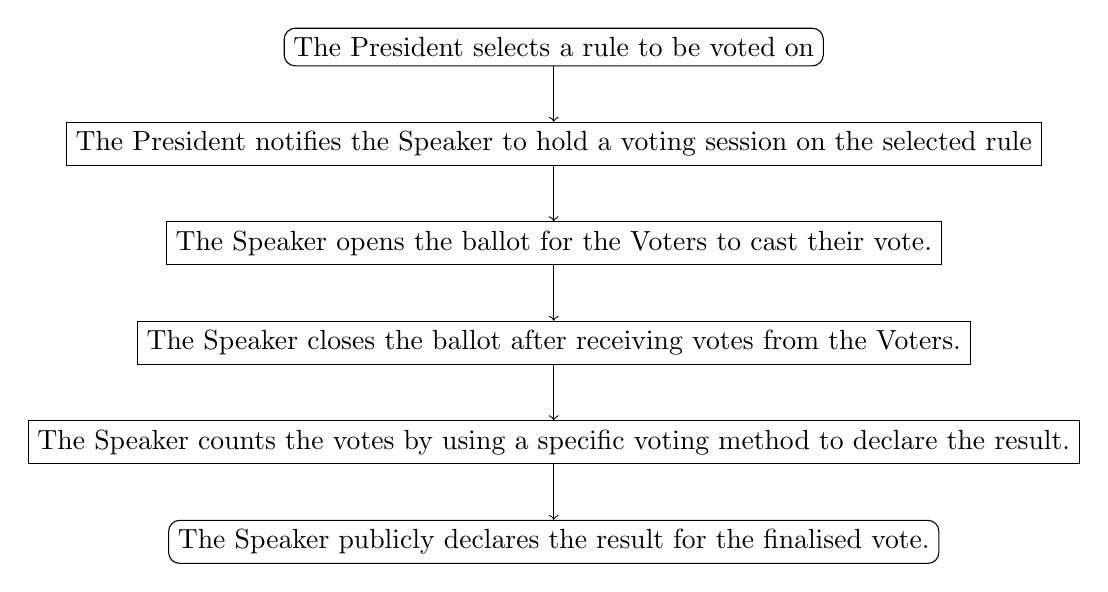
\begin{tikzpicture}[node distance=20pt]
\centering
\node[draw, rounded corners] (start)  {The President selects a rule to be voted on};
\node[draw, below=of start] (step 1)  {The President notifies the Speaker to hold a voting session on the selected rule};
\node[draw, below=of step 1] (step 2)  {The Speaker opens the ballot for the Voters to cast their vote.};
\node[draw, below=of step 2] (step 3)  {The Speaker closes the ballot after receiving votes from the Voters.};
\node[draw, below=of step 3] (step 4)  {The Speaker counts the votes by using a specific voting method to declare the result.};
\node[draw, below=of step 4, rounded corners] (end)   {The Speaker publicly declares the result for the finalised vote.};
 \draw[->] (start)  -- (step 1);
 \draw[->] (step 1) -- (step 2);
 \draw[->] (step 2) -- (step 3);
 \draw[->] (step 3) -- (step 4);
 \draw[->] (step 4) -- (end);
\end{tikzpicture}
\caption{Voting Protocol for Rules}
\label{fig:RONRVotingProtocol}
\end{center}
\end{figure}

For elections of roles, the sequence of actions of the voting protocol is mostly similar to the above explanation in principle, except for some parameters, such as the motion of the vote which is the role itself (President, or Speaker, or Judge), the facilitator of the election/vote event which depends on what role is being held for election (refer to Chapter 5 IIGO for more details on change of roles and power transfer), and the applicable voting method function to call for election that will produce the result, which is different from the voting method used for rules. Refer to Section~\ref{sec:VotingMethods} for more details on voting methods to be used for elections of roles.

At the start of the game, it is assumed that all 6 islands have the power to vote at any necessary voting scenario, and no diplomatic sanction is in place for any island. However, in the further turns of the game, some island(s) could lose their right to vote and/or not permitted to participate in a voting event due to the diplomatic sanction(s) in place. Refer to Chapter 5 IIGO for details on diplomatic sanction. In this case, the Speaker will open the ballots to the eligible islands only , i.e. those who are permitted to vote at a certain state of the game.

% Implmentaion section deleted
\begin{comment}
\section{Implementation}
\label{sec:Implementation}

\subsection{Voting for Rules}
\label{sec:VotingForRules}
The implementation of voting for rules from infrastructure point of view (file:\texttt{rulevote.go}) basically follows the sequence of voting protocol as described in Section~\ref{sec:VotingProtocol}. At initialisation, there are two defined structs (collection of data fields) that are used as parameters for functions inside the voting algorithm, such as \texttt{RuleVote} and \texttt{BallotBox}. The \texttt{RuleVote} struct consists of 3 variables, i.e. \texttt{ruleToVote} (string) that contains the rule that has been selected by the President to be voted on, \texttt{islandsToVote} (list of integers) that contains a list of \texttt{ClientID} which indicates all eligible islands that participate in the voting session, and \texttt{ballots} (list of boolean) that contains the vote of each respective eligible islands where it can indicate the vote for in-favour or against the proposed rule. The \texttt{BallotBox} struct consists of 2 integer variables that act as accumulators for the count of each possible vote: \texttt{VotesInFavour} and \texttt{VotesAgainst}.

According to Section~\ref{sec:VotingProtocol}, The Speaker firstly starts a voting session by calling \texttt{SetRule(rule)} function that contains the rule selected by The President to be voted on. Next, the Speaker sets all eligible islands that can participate/have the right to vote in the voting session at that state of the game by using \texttt{SetVotingIslands(clientIDs[])} function. After that, the Speaker opens the ballots to get the votes from all eligible islands by calling \texttt{GatherBallots(clientMap[ClientID])} function. Subsequently, the \texttt{GetBallotBox()} function is called by the Speaker to gather the ballots that already contain the votes counting of those who are in-favour or against the proposed rule. Finally, the votes counting is concluded by comparing the votes of those in-favour vs those against, and the in-favour votes win when the counting is greater than or equal to the against votes counting, as reflected in \texttt{CountVotesMajority()} function. The Speaker then uses this result to declare the result of this voting session in IIGO.

\subsection{Elections}
\label{subsec:Elections}
The elections for roles implementation can be seen in the file:\texttt{election.go}. At initialisation, there is a defined struct \texttt{Election} that contains 4 parameters, i.e. \texttt{roleToElect} that indicates which role is being voted on (President, or Speaker, or Judge), \texttt{votingMethod} that indicates the voting method being used for the election to determine the winner selection, \texttt{islandsToVote} that contains a list of \texttt{ClientID} which indicates all eligible islands that participate in the voting session, and \texttt{votes} that is a list that contains the order rank of preference of the candidates for the role from each eligible island who casts the vote.

The election session begins by calling the \texttt{ProposeElection(role,method)} function that depends on which role being voted on and which role has obligation to facilitate the election (refer to Chapter 5 IIGO on Change of Roles and Power Transfer sections), and the selected voting method to be used for this election (refer to Section~\ref{sec:VotingMethods} for details on voting methods and Subsection~\ref{subsec:VotingPseudo} for pseudo-code implementation). The election facilitator then opens ballots to all eligible islands to cast their votes by calling \texttt{OpenBallot(clientIDs[])} function. The \texttt{Vote(clientMap[ClientID])} function gathers all the ballots containing the votes from all eligible islands that are obtained from \texttt{GetVoteForElection(roleToElect)} function returned from each client/island code execution. After that, the election facilitator closes the ballots by using \texttt{CloseBallot()} function and it returns the result of the votes counting using the selected voting method by calling each respective voting method function. This result is used by the election facilitator to declare the winner for the elected role. By default, the voting method for election is Borda Count and the function is called \texttt{bordaCountResult()} where the algorithm follows through what are explained in Section~\ref{sec:VotingMethods} and Subsection~\ref{subsec:VotingPseudo} where the Borda scores will be calculated based on the order rank of preference of the candidates from each ballot. The other voting methods can be used for election and it is selected by the election facilitator.

\subsection{Voting Methods Implementation Pseudo-code}
\label{subsec:VotingPseudo}

\textbf{Plurality}
\newline
Call for Voting inputs (int:IslandID, str:"Aye", "Nay" or "Abstain")\\
\begin{algorithm}[H]
\ForEach{$ballot \in ballots $}{
    \If{$Aye$} {Count for $Aye ++ $}
    \If{$Nay$} {Count for $Nay ++ $}
}
\If{$Aye > Nay$}{\Return the Winner: $Aye$}
\Else{\Return the Winner: $Nay$}
\end{algorithm}

\ \newline \ \newline \ \newline
\textbf{Borda Count}
\newline
\begin{algorithm}[H]
\For{all ballot}{
    $numNotIn\gets N-ballot.length$\\
    $shareScore\gets 1+...+numNotIn$\\
    \For{i from 0 to N-1}{
    \If{i is in ballots} {$scores[i]\gets scores[i]+N-K+1$ }
    \Else {$scores[i]\gets scores[i]+shareScore/numsNotIn$ }
    }
}
Sort candidates by Borda scores\\
\Return the candidate with the highest score
\end{algorithm}

\ \newline \ \newline \ \newline
\textbf{Runoff}
\newline
\begin{algorithm}[H]
\For{All $ballot \in ballots $}{
    Select two candidates with most first-placed votes
}
\If{either already has a majority}{
\Return the majority one}
\Else{Each voter selects one candidate of the top 2\\
}
\Return the candidate with the most votes
\end{algorithm}

\ \newline \ \newline \ \newline
\textbf{Instant Runoff}
\newline
\begin{algorithm}[H]
\ForEach{$ballot \in ballots $}{
\For{i from 0 to N-1}{
\If{i is first choice}{$scores[i]\gets scores[i]+N-K+1$}
}
}
\If{candidate in ballots $>1$}{
Remove the candidate with the fewest first
choice votes from the ballots.\\
GOTO the top for next round of counting
}
\Else{\Return the candidate}
\end{algorithm} 

\ \newline \ \newline \ \newline
\textbf{Approval}\\
\begin{algorithm}[H]
\ForEach{$ballot \in ballots $}{
    \For{i from 0 to N-1}{
    \If{i is in ballot} {$scores[i]\gets scores[i]+1$ }
    }

}
Sort candidates by scores\\
\Return the candidate with highest score
\end{algorithm}
\end{comment}
    \chapter{Team 1 Agent Design}

\section{Core Idea}
Team 1 agent was designed around the idea that the agent wants the whole archipelago to survive. However, the agent does have different configurations to allow for some malicious behaviour in order to facilitate some interesting agent interactions.

\section{Emotional state}

The agent's behaviour is affected by what we have termed her \emph{emotional state}. This is governed by the agent's current resources in relation to the living cost.

\begin{table} [htb]
    \centering
    \begin{tabular}{|l|l|}
        \hline
        \textbf{Emotional State} & \textbf{Condition} \\
        \hline
        Happy & Default state \\
        \hline
        Anxious & Current resources under 5 times the living costs \\
        \hline
        Desperate & Agent in critical state \\
        \hline
    \end{tabular}
\end{table}


\section{Opinions on Islands}
As information and resource sharing between islands is possible, it is possible and desirable for the agent to form an opinion of other islands. This be used to gauge the accuracy of information from other islands as well as, potentially, deny resource sharing to islands deemed ``selfish''.

Initially, opinion on all islands is neutral. Over time, through IITO and IIGO, opinions on islands will change. This will affect behaviour in IITO, as well as IIGO voting. Note that positive values correspond to positive opinions while negative values correspond to negative opinions.

\section{IITO Gifts}
When team 1 agent receives a request for gifts, the agent will decide how much to offer depending on the agent's current emotional state and the opinion of that island.

\begin{table} [htb]
    \centering
    \begin{tabular}{|c|p{0.5\textwidth}|}
        \hline
        \textbf{Emotional State} & \textbf{How is IITO handled?} \\
        \hline
        Happy & Agent will give away resources that satisfies the requested amount. Up to a percent of available resources. \\
        \hline
        Anxious & Agent will give away a ratio of the requested amount and its current resources. \\
        \hline
        Desperate & Agent will refuse any gift requests that it receives. \\
        \hline
    \end{tabular}
\end{table}

During IITO, the agent's opinion of other islands is affected. For every gift received, the agent's opinion of the gift-giver increases. However, the agent's opinion of an island can decrease if that island promised a gift and did not fulfil it.

Moreover, if the agent's opinion of an island is very high, the agent can decide to give gifts disregarding the agent's own anxiety. On the other hand, if an opinion of an island is very low, the agent can decide to refuse to send a gift even though the agent is happy.

For increase survivability, team 1 agent will accept any gift offers that it receives.

\subsection{Future Work}
Team 1 agent currently has a very straightforward IITO strategy. Possible alteration to this strategy could include:
\begin{itemize}
    \item Being less susceptible to bribery. The agent should stop increasing the opinion of an island after receiving $X$ amount of continuous gifts.
    \item Stop handing out gifts to islands that are not in critical state.
    \item Being proactive in bribery. The agent will give non-requested gifts to the current president in hopes that this will reduce tax and increase resource allocation from the common pool.
\end{itemize}

\section{IIFO Disaster Prediction}
Disasters can happen deterministically or stochastically (see Chapter~\ref{sec: Disaster} for more information). For an agent, it is important to predict when a disaster occurs so that as much disaster damage is mitigated using the common pool.

When the game starts, the disaster prediction made by the agent is random. This prediction always has a confidence value of $0$. As more disasters occur, a history of disasters is built up. Using this history, the mean disaster position ($x$, $y$), magnitude and period is calculated. A confidence value is calculated along with the mean disaster metrics and shared along with the prediction.

% Add a footnote on website?  https://www.mathsisfun.com/data/confidence-interval.html
The confidence value is calculated by finding the ratio between margin of error and the mean value. The smaller the margin of error, the more confident the agent is in her prediction. Therefore, a difference between the mean value and the margin of error must also be calculated. The confidence interval equation is used to calculate the margin of error:

\begin{equation}
    \label{eq: Team1MarginOfError}
    \textsc{Error} = Z \dfrac{s}{\sqrt{n}}
\end{equation}

where $s$, $n$ and $Z$ are the standard deviation, size of array and confidence interval respectively.

Using the difference between the mean value ($\bar{x}$) and the margin of error and taking the ratio of this result over the mean will provide the agent with the confidence value.
\begin{equation}
    \textsc{Confidence Value} = \frac{\bar{x} - \textsc{Error}}{\bar{x}}
\end{equation}.

The agent maintains a \textbf{trust score} for every island \emph{including itself}. This is based on the accuracy of islands' prediction of time left to the disaster.

Sharing and obtaining other disaster information to and from other islands respectively can increase the survivability of the archipelago. As more disaster predictions are shared, a network of trust between team 1 agent and other islands is built.

\subsection{Future Work}
While team 1 agent has a satisfactory disaster prediction algorithm, it does not make use of this prediction or predictions from other islands in any meaningful way. This is primarily due to disaster prediction being one of the last features to be implemented and not enough time being available to complete it.

Nevertheless, here are some possible uses for the disaster prediction system.

\begin{itemize}
  \item \textbf{Tax policy} --- As president, the agent could choose to increase or decrease taxation depending on (predicted) time left to disaster.
  \item \textbf{Voting} --- A trustworthy island could make for a better president, speaker or judge, as they would be able to act according to imminent disasters.
  \item \textbf{Common pool contribution} --- Based on predicted disaster location the agent may increase or decrease her common pool contribution. If a disaster is expected to affect the agent significantly then she could choose to mitigate resource loss by contributing a large amount to the common pool, as the alternative would be losing more resources.
\end{itemize}

Finally, prediction accuracy could be improved by using the prediction of the most trustworthy island, whether that is the agent herself or not, or averaging the predictions of the most trustworthy islands.

\section{IIGO: President}

Following the agent's core idea, as the president, the agent will try to enlarge the common pool as well as redistribute wealth among the islands, in an attempt to ensure the survival of as many islands as possible. This is achieved through an aggressive, tiered tax policy as well as denying common pool allocation requests to the wealthier islands.

This policy had to be verified as it could be vulnerable to ``free-rider'' islands, who could avoid paying tax and still reap the benefits of disaster protection from a large common pool and ``bailout'' allocations when they are low on resources.

As a test of this, a simulation was set up with a variable number of lawful and free-rider islands in order to measure the stability of this policy.

Three tax evading islands (half of the islands) was found to be the limit at which this policy would lead to collapse of the IIGO and the common pool. This was deemed an acceptable limit as at least half of the other agent teams would obey tax policy, at least most of the time or with a small amount of evasion. The resource graphs for the cases of two and three tax evading islands can be seen in \autoref{fig:team1:two_invaders} and \autoref{fig:team1:three_invaders}.

\begin{figure}[H]
\centering
\includegraphics[width=0.9\textwidth]{09_team1_agentdesign/images/two_invaders}
\caption{Resource graph. Islands 5 and 6 are evading tax.}
\label{fig:team1:two_invaders}
\end{figure}

\begin{figure}[H]
\centering
\includegraphics[width=0.9\textwidth]{09_team1_agentdesign/images/three_invaders}
\caption{Resource graph. Islands 4 to 6 are evading tax.}
\label{fig:team1:three_invaders}
\end{figure}

Note here that collapse of IIGO (as in \autoref{fig:team1:three_invaders}, with three tax evaders) does not automatically imply collapse of the archipelago; the islands appeared to survive (and, in fact, thrive) even after the collapse of IIGO.\@ It was taken as an assumption that this was only due to the uniformity of strategies, and in the ``real'' simulation, with heterogeneous agents, collapse of IIGO would lead to collapse of the archipelago.



\section{Foraging}
Multiple foraging strategies were developed, initially by intuition and later by attempting to address the shortcomings of previous attempts. They were developed in order and aptly named:
\begin{itemize}
    \item Return on Investment (ROI)
    \item Regression
    \item Flip Forage
\end{itemize}


\subsection{Return on Investment (ROI) Foraging}%
\label{sec:forage-roi}

This first algorithm is based on repeating successful foraging behaviours in the past, whether those be by the agent herself or another agent.

For the first few turns (the exact amount is configurable) the agent will forage randomly.

The agent maintains a history of foraging decisions and outcomes, including those received from IIFO.\@ When it comes time to forage, this history is sorted by ROI, i.e.\ the ratio of profit to contribution. Decisions that resulted in a loss, had profit smaller than the living cost, or had a larger contribution than a (configurable) percentage of available resources, are filtered out.

\subsection{Regression Foraging}%
\label{sec:forage-regression}

This strategy tries to predict the ideal foraging decision, even if that exact decision was not made in the past. This is done using regression, which is used to find the decision with the highest expected reward.

The \emph{regression} strategy forages randomly in the initial turns and history is kept as in \nameref{sec:forage-roi}. To make a foraging decision, the history is split by foraged resource (fish or deer), and quadratic regression is performed on contribution versus reward for both resources. From this, a quadratic equation is formed. If the quadratic equation found is negative then the optimal contribution can be found by differentiation. If it is positive then a (large) value is chosen as contribution, as a higher contribution should simply lead to a higher reward.

\subsection{Flip Foraging}

This strategy chooses the least foraged resource from the last turn, according to IIFO-reported data. Contributed amount is proportional to the chosen resource's total ROI from last turn. This choice was made under the assumption that ROI is an indicator of the resource's ``condition''. If a resource only gives moderate rewards (proportionally to input) it means that it is probably over-used currently and as such agents should allow it to recover, by scaling down their foraging attempts or by switching foraging types.

\subsection{Comparison}

To compare the three strategies, simulations were run with six agents, two using \emph{ROI foraging}, two using \emph{regression foraging}, and two using \emph{flip foraging}. IIGO and IITO were also disabled in order to isolate the efficacy of foraging methods from other parts of the game. The simulation was run five times and the results averaged over the 5 games as well as the two agents following the same strategy.

\begin{figure}[H] 
\centering
\includegraphics[width=0.6\textwidth]{09_team1_agentdesign/images/mean_survival_turns}
\caption{Mean survival turns for different strategies.}
\label{fig:team1:mean_survival}
\end{figure} 

\begin{figure}[H] 
\centering
\includegraphics[width=0.6\textwidth]{09_team1_agentdesign/images/total_efficiency}
\caption{Average foraging efficiency}
\label{fig:team1:average_efficiency}
\end{figure} 

It is clear from \autoref{fig:team1:mean_survival} that the \emph{flip} foraging strategy dominates the other two in terms of overall effectiveness. However, it is interesting to note that, according to \autoref{fig:team1:average_efficiency}, the \emph{ROI} foraging method is almost as efficient as \emph{flip}, which raises the question of what causes the difference in their success. This difference could be attributed to one core issue with the \emph{ROI strategy}: ignoring the absolute value of rewards. The agent will happily settle for a profit of $11$ resources, if that was obtained with a contribution of $0.1$ resources (a profit of $110000\%$) over a profit $50$ resources for a contribution of $25$ (a measly $100\%$). This means that in the long run living costs overwhelm the \emph{ROI} agent. The \emph{flip} agent does not take expected profit into account and as such is unaffected by this.

\emph{Regression} appears to occupy a medium between \emph{flip} and \emph{ROI}, however it is much less consistent, as evidenced by the error bars in \autoref{fig:team1:mean_survival}, with \emph{regression} surviving for under 10 turns in some runs.

%%% Local Variables:
%%% mode: latex
%%% TeX-master: "../main"
%%% End:

    \chapter{Team 2 Agent Design}
\section{Overall Agent Strategy}

The overall strategy of our agent is based on a series of distinct, overlapping dilemmas. The agent operates on principles based on Evolutionary Economic Theory \footnote{https://www.cambridge.org/core/what-we-publish/elements/evolutionary-economics}. Game theory and the use of the Nash equilibrium also guided the development of the strategies implemented. The other top-level strategy which overlaps with several dilemmas is the social dilemma; this is when we quantify the relationship we have with other agents to produce trust and confidence levels. The interaction between the top-level strategies with all of the dilemmas is shown in Figure~\ref{fig: top level strategy}. The top-level strategy's implementation into each agent function and role is discussed in the following sections. 

\begin{figure}[!htb]
    \centering
    \subfigure[Top level strategy]{
        \centering
        \includegraphics[width=0.49\textwidth]{10_team2_agentdesign/images/strategies.png}
        \label{fig: top level strategy}    
    }
    \subfigure[Ceremonial-Instrumental dichotomy]{
        \centering
        \includegraphics[width=0.49\textwidth]{10_team2_agentdesign/images/dichotomy.png}
        \label{fig: dichotomy}
    }
\end{figure}

\subsection{Evolutionary Economic Theory}
The term Evolutionary Economic Theory was first coined by economist Thorstein Veblen \footnote{https://www.cambridge.org/core/what-we-publish/elements/evolutionary-economics}. Evolutionary Economic Theory proposes that economic processes evolve, and it rejects the assumptions of classical rational choice theory. From Evolutionary Economic Theory, we categorised agent behaviour into distinct groups \footnote{https://www.cambridge.org/core/what-we-publish/elements/evolutionary-economics}. These groups are an altruist, fair sharer, and free rider. These are explained in Table~\ref{tab:Evolutionary Economic Theory Agent classifications}.


\begin{table}[!htb]
    \caption{Evolutionary Economic Theory Agent classifications}
    \label{tab:Evolutionary Economic Theory Agent classifications}
    \begin{tabular}{|c|m{0.3\textwidth}|p{0.4\textwidth}|}
    \hline
    \textbf{Agent classification} & \textbf{Definition}  & \textbf{Examples within the game} \\ \hline
    Altruist  & More concerned about the welfare of the group than themselves  & \begin{tabular}[p{0.4\textwidth}]{@{}p{0.4\textwidth}@{}}-Contributes a surplus to the common pool\\ -Generous with gifts\end{tabular}                                                     \\ \hline
    Fair Sharer                   & Contributes enough to the group  to negate their negative impact on it & \begin{tabular}[p{0.4\textwidth}]{@{}p{0.4\textwidth}@{}}-Contributes the minimum necessary amount of resources \\ -Gift allocation is measured and reasonable\end{tabular}                          \\ \hline
    Free rider                    & More concerned with their individual welfare than the welfare of the group & \begin{tabular}[p{0.4\textwidth}]{@{}p{0.4\textwidth}@{}}-Will not contribute enough to the common pool \\ -Gift requests above their requirement \\ -Will not give out gifts\end{tabular} \\ \hline
\end{tabular}
\end{table}
    

The advantage of using this theory over rational choice theory from classical economics is that it accounts for the irrational decisions agents or humans make when dealing with economic decisions, such as deciding how much to contribute to a common pool. Humans have evolved to develop heuristics \footnote{\url{https://www.sciencedirect.com/topics/social-sciences/heuristics}} which are "rules of thumb" in order to make economic decisions quickly and when all information is not present. These heuristics are typically based on emotion and will often result in irrational decisions; an example of this would be brand loyalty. This is very relevant within the context of the game because there is a cost to large computations (decision making). Also, there is an information failure \footnote{\url{https://www.economicsonline.co.uk/Market_failures/Information_failure.html}} as the agents often do not know the threshold of the common pool and other vital game metrics. This information failure forces agents to use heuristics similar to those used by real people. An excellent example of a heuristic within this agent strategy is the level of trustworthiness decided within the social dilemma. If every agent was rational and all information was present in the game, there is no need to trust or distrust agents as they would maximize both their welfare and that of others.

Another primary reason for selecting this theory as the basis of our design is to explore the ceremonial-instrumental dichotomy\footnote{\url{https://www.jstor.org/stable/3486187?seq=3\#metadata_info_tab_contents}}. This dichotomy is best represented by the graph in figure \ref{fig: dichotomy} and shows the importance of the game's setup. Our agent is attempting to oppose this traditional response to instrumental and ceremonial societies. It would be interesting to change the game's ceremonial and instrumental values by changing the setup. While the current game infrastructure does not support this, it would be interesting to investigate the ceremonial-instrumental dichotomy by allowing islands to invest resources into developing their foraging technology to obtain higher returns. It would be interesting to investigate how this instrumental shift would change our agent's strategy and others' actions. This update in technology would replace the ceremonial institutional set up of the IIGO as it becomes redundant. Allowing islands to invest in technological advancement would add an extra dimension to the game as it evolves, and the importance of the IIGO and other instrumental components would shift.

\subsection{Evolutionary Economic Theory Implementation}
%explain how we use the information from the theory

Figure~\ref{fig:methods-of-play} shows the different states of our agent's different methods of play. At any point during the game, the state of our agent is determined only by the level of the Common Pool. Our agent's objective is to oppose the strategies employed by other agents to attain stability in the game. To determine the method of play of the other agents, we look at whether the Common Pool is, on average, increasing or decreasing. If the pool is being depleted, it can be assumed that the other agents act as free-riders on average. To counteract this, we act as an altruist (see section \ref{sec:Common Pool Dilemma Strategy} for more detail). The average pool level is used because individual agent strategies are irrelevant for the game's overall course. Within the game, we also do not always have access to individual agents' contributions, which would be needed to classify them individually. This makes the average level of the Common Pool the only viable parameter. 

Our simulations demonstrated that starting the game in a "free-rider" state resulted in optimal agent performance and did not negatively impact the course of the game overall.

The default state for the agent is to be a "fair sharer." The agent will move into altruist mode when the weighted average of the Common Pool has dropped drastically. The agent considers a weighted average to ensure that the agent does not panic after every disaster and over contribute. The most recent turns will also be weighed higher to determine the course of the game. When the Common Pool stops decreasing, the agent will move back to fair sharer mode. Similarly, if the pool's weighted average increases by a large factor, then our agent moves into a free-rider state.

\begin{figure}
    \centering
    \subfigure[Method of Play diagram]{
    \centering
        \includegraphics[width=0.4\textwidth]{10_team2_agentdesign/images/MethodofPlay.png}
        \label{fig:methods-of-play}
    }
    \subfigure[Social Classification Order]{
    \centering
    \includegraphics[width=0.4\textwidth]{10_team2_agentdesign/images/Social.png}
    \label{fig:social-order}
    }
\end{figure}



\subsection{Social Classification}
The agent forms an opinion on others depending on different situations. Initial testing suggested that another island's gift-giving behaviour does not necessarily correlate with their quality of predictions. Consequently, the trust of other agents is computed and stored separately for each situation. The agent uses the weighted average of past interactions with other agents to determine whether to trust them in each situation for future interactions. Using a weighted average to compute trust resulted in notably better agent performance. This is because the agent's trust in other agents considers all interactions with other agents while weighting recent interactions more heavily.

An integer value represents the agent's trust metric for each agent in each situation between 0 and 100, where 100 denotes full confidence and 0 a complete lack thereof. This value is used to compute the expected outcomes of situations. These are then compared with real events to update the agent's confidence in the other agents regarding this situation. For example, when the agent receives predictions from other islands, it computes the weighted average to check whether it trusts the island. Once a disaster occurs, the magnitude or timing of the disaster is compared with the other island's prediction. This reality is used to assess their behaviour and update the trust metric for that island relating to that situation. The list of different "situations" includes how an agent behaves in a role such as the President, Judge, Speaker, gift-giving, and disaster prediction. The overall structure of how the agent forms opinions on other islands is shown in Figure~\ref{fig:social-order}.

\section{Gift Giving and Receiving}
The agent must decide whether or not to respond to other agents' gift requests and how much to request from others through gifting. The implementation does not consider whether or not an agent is critical when requesting gifts and instead considers its current method of play and the trustworthiness of the requesting agent. Figure~\ref{fig: gifts} shows a decision tree for how the agent will allocate or request gifts, in which the agent splits up the gift request among the other agents to increase the likelihood of an agent allocating the gift.


\begin{figure}[!htb]
    \subfigure[Gift Giving and Receiving decision tree]{
        \centering
        \includegraphics[width=0.49\textwidth]{10_team2_agentdesign/images/gifts.png}
        \label{fig: gifts}
    }
    \subfigure[Common Pool Strategy]{
        \centering
        \includegraphics[width=0.49\textwidth]{10_team2_agentdesign/images/common_pool_strategy.png}
        \label{fig: common_pool_strategy}
    }
\end{figure}



Depending on the method of play, the agent will request more or fewer gifts. This is inversely proportional to the number of resources taken from the Common Pool. The agent obtains a larger proportion of its needed resources from gifting than the Common Pool in the altruist state. This is done to mitigate common pool depletion in the interest of the common good. In a Fair-Sharer state, the agent aims to obtain its resource target equally from gifts and the Common Pool. A minor surplus is also included in the resource target to ensure that the goal is met, given that gifts from other agents cannot be guaranteed. In a Free-Rider state, the agent takes the majority of its resources directly from the Common Pool but still requests gifts to build up its resources by taking advantage of relationships with other agents as well as a Common Pool surplus.

The \textbf{Gifts} social classification situation refers to both when an island requests a gift from our agent and when our agent requests a gift from that island. The balance between agent gift requests and responses is used as a basis for opinion formation on another agent. Other agents that fulfill the agent's requests are rewarded with higher trust. The agent's own gift requests tend to be small but are also proportional to its trust in each other agent. Every gift interaction is used to update the agent's trust in another island's gifting behaviour.

\section{Common Pool Dilemma Strategy} \label{sec:Common Pool Dilemma Strategy}
The Common Pool dilemma strategy can be split into two considerations. One consideration is the current method of play (altruist, fair sharer, and free-rider), and the other is the current game state. A decision tree showing the common pool strategy is shown in Figure~\ref{fig: common_pool_strategy}. These considerations decide whether and how much we contribute or take from the Common Pool.

\subsection{Method of play consideration} \label{ssec:Method of play consideration}
The primary consideration for giving to the Common Pool dilemma is the agent's current method of play. The agent's state is determined by the Common Pool level, as seen in Figure~\ref{fig:methods-of-play}. The agent's default state as a "fair sharer" contributes the average amount of other agents to the Common Pool. This is calculated by evaluating changes in the Common Pool level from the previous turn and averaging this quantity by dividing by the number of alive agents. If the Common Pool level decreases, the most recent Common pool increase is used to determine the amount given.

By using the average Common Pool contribution, the agent benefits from the forecasting of other agents. This benefit would arise should another agent have an advanced forecasting prediction that determines the Common Pool threshold and what is required to mitigate the effects of a disaster. In this case, the agent would then contribute a similar quantity of resources. This "herd-mentality" approach relies on the assumption that other agents make rational decisions. So if it is evident that other agents are acting irrationally, the agent deviates from this approach to an alternative state (to become either a free-rider or an altruist).

The agent is in an altruist state when the Common Pool is struggling, which often means that other agents act as free-riders. This is where the meta-strategy of Evolutionary Economic Theory comes into play. It is in the agent's interest to contribute much more to the Common Pool to alter the game's course in a positive direction and prevent the pool from being below the threshold when a disaster occurs. Therefore, the agent contributes more resources to enact this balance on the system. 
The altruist resource contribution is a larger factor of the weighted average contribution and can be tuned using the \emph{altruist factor} variable in the agent's configuration.

In a free-rider state, the Common Pool has a surplus, and the agent assumes other agents are on average operating as altruists. In this situation, the agent contributes less to the Common Pool and preserves resources to mitigate short and long-term risk. Contributing too much to the Common Pool no longer benefits the greater good, as these resources can still be used to forage and generate more resources. Therefore, the agent accumulates resources when others are too generous, allowing greater foraging investments and making it easier to help other agents if they struggle in the future.

The method of play also impacts how the agent decides to take from the Common Pool. After game state considerations are made, the agent adjusts how much it takes from the Common Pool according to its Agent State. Table~\ref{tab:Method of play common pool taking} outlines a summary of how the agent adjusts how much it takes and gives a justification for each action. The amount to take from the pool depends on how willing other agents are to contribute to the agent within the game's gift-giving section.  This means the agent must decide what proportion of the resource request must be taken from the Common Pool and from gifting, and this decision also factors in both common pool allocation as well as gift response predictions. When the agent is in a free-rider state, the common pool has a surplus, and so it makes more sense to take directly from the pool rather than requesting gifts. 

\begin{table}[!htb]
\centering
\caption{Method of play common pool taking}
\label{tab:Method of play common pool taking}
\begin{tabular}{|c|c|}
\hline
\textbf{Agent classification} & \textbf{How this impacts taking from the common pool}                              \\ \hline
Altruist                      & Pool is being depleted, best to not take from the pool                             \\ \hline
Fair Sharer                   & Gift requests and taking from the pool are equal                                   \\ \hline
Free rider                    & \multicolumn{1}{l|}{Pool has surplus, take from the pool rather than gift request} \\ \hline
\end{tabular}
\end{table}

\subsection{Game state consideration} \label{ssec:Game state consideration}
The primary consideration in taking from the Common Pool is the current game state. The key parameters (shown in Figure~\ref{fig: common_pool_strategy}) considered are whether the agent is critical and whether the agent has excess resources. This excess is calculated as the difference between the agent's current resources and the minimum resource threshold and the cost of living. Beyond this minimum resource level, the agent can survive one another turn. If the agent has fewer resources than these aggregated costs, the excess is zero. If there are excess resources, the agent will give some resources to the Common Pool. In this case, a strategic contribution is calculated. If the Common Pool threshold is known, the agent considers how many resources are required to attain this threshold. This is then spread over the expected number of turns until the next disaster is predicted to occur and the number of alive clients. If this is unknown, a default value is used to form an initial guess in the agent configuration. On top of this quantity, a strategic contribution is also calculated (see \ref{ssec:Method of play consideration}). The current method of play determines whether the disaster-determined contribution or the strategy-determined contribution is contributed to the pool. This amount is then contributed together with the current tax, unless there are no excess resources as this implies the agent is in a critical state and so all resources are preserved.

\section{Foraging Dilemma}
The foraging dilemma is split into two parts. One determines whether the agent should hunt or fish, and the other determines how many resources to spend on foraging. The foraging dilemma only depends on the current method of play. The method of play will impact the amount the agent uses to forages. If the Common Pool is doing well and the agent acts as a free rider, it will be more prone to take risk and contribute more to the foraging and vice versa. The decision to hunt or fish depends on the likely number of hunters in the next foraging event. The decision tree, Figure~\ref{fig: Hunt or fish decision tree }, shows how the agent decides whether to hunt or fish in a given turn. To determine the number of hunters in the next forage turn, the agent tracks how often each agent is a hunter and then sums up the probability of each agent hunting to find an overall number of likely hunters. The agent outputs a random number from 0 to 1, and if the number lies above the threshold, the agent will hunt. This threshold is determined by the number of likely hunters in the foraging. It implies there is an element of randomness to the agent's decision making, which will account for the unpredictability of dealing with other agents with their strategies.

\begin{figure}[!htb]
    \centering
    \subfigure[Hunt or fish decision tree]{
        \centering
        \includegraphics[width=0.4\textwidth]{10_team2_agentdesign/images/forage_decision.png}
        \label{fig: Hunt or fish decision tree }
    }
    \subfigure[Roles Decision Tree]{
        \centering
        \includegraphics[width=0.4\textwidth]{10_team2_agentdesign/images/Roles Decision Tree.png}
        \label{fig: Roles Decision Tree}
    }
    \caption{Hunting or Fishing and Roles Decision Tree}
\end{figure}



The ideal distribution for foraging is to have two agents hunting and the remainder fishing. Hence, when the agent predicts one other agent will hunt, the agent is highly likely to choose to hunt too. The default threshold for hunting is 0.1, so the agent will hunt 10\% of the time when not considering the likely number of hunters. By assuming that any agent will hunt or fish with equal probability, the likelihood that there is one hunter is approximately 0.16. This implies hunting is an optimal strategy approximately 16\% of the time, so a threshold similar to this value is chosen. If the predicted number of hunters is above one, the following equation is used to determine threshold placement: $\text{Probability of agent hunting} = 0.95 - \text{Predicted number of hunters} \times 0.15$

The probability of choosing to hunt when the agent is confident only one other agent will also select hunt is 0.95. For each additionally predicted hunter, the probability will fall by 0.15. This 0.95 threshold is included in the agent configuration so it can be edited without changing the code. Hence, the foraging decision can be tuned. The agent checks if there are any excess resources after considering the minimum resource threshold not to be critical and the cost of living. If there are no excess resources, no resources are spent on foraging. If there is an excess of resources, a percentage of this excess is used on foraging. This percentage is controlled in the agent configuration. This approach ensures the agent has enough resources to survive another round, even in the worst case scenario when foraging returns are minimal.

\section{Role Strategies}

Figure~\ref{fig: Roles Decision Tree} shows a decision tree of how the agent acts under the two roles implemented. Due to time constraints, the base client implementation was used for the Speaker. The President is responsible for allocating resources from the Common Pool based on agent requests. The agent uses game state variables such as their critical status to determine if another agent is worthy of their resource request and the agent's allocation method based on the method of play is outlined in Table~\ref{tab:President allocation method of play}. When the agent is in a free-rider state, it is more selfish, while when it is an altruist, more of the others agents requests are approved. If an agent is not critical, it is highly unlikely that the agent will allocate them their requested resources as the purpose of the Common Pool should be to primarily mitigate the effects of disasters. Resources are allocated on a need-first basis, taxed proportionally to an agents resource level, and the strategy to determine taxation includes an additional penalty tax for agents who do not declare their resource levels. When evaluating another President's performance, the agent considers the percentage change in tax, the percentage of how much the agent is allocated with respect to how much it requests, and how much the agent takes with respect to how much the President allocates it.

\begin{table}[!htb]
\centering
\caption{President allocation method of play}
\label{tab:President allocation method of play}
\begin{tabular}{|c|c|}
\hline
\textbf{Agent classification} & \textbf{\% of request given} \\ \hline
Altruist                      & 60                           \\ \hline
Fair Sharer                   & 50                           \\ \hline
Free rider                    & 40                           \\ \hline
\end{tabular}
\end{table}

The agent implementation of the Judge evaluates whether an agent has broken any rules, as it should. However, to model real world corruption, the agent does not sanction agents that break rules if it considers them to be highly trustworthy (i.e., with a trust score above 80\%). The agents behaviour as a Judge is also determined by its state; when the agent is a free-rider, it sanctions fewer islands. The \textbf{Judge}'s situation, similar to the President, is used by the agent to determine what island to vote for as Judge. This is done by checking the past sanctions the agent received and their duration, to maxmimise personal benefit. The \textbf{RoleOpinion} social classification situation is used when the agent is the Judge and must decide whether or not to pardon other islands' sanctions, whom to choose as the next President whether or not an island has adhered by the rules. The Judge receives information for each island, such as the difference between how much an island contributed to the common pool and how much said they would. The agent uses these differences as a Judge to determine whether or not an island is trustworthy. During a role election, the agent checks its trust in the candidates for the appropriate situation, i.e., the situation when an agent is "President" for a future Presidential election. The agent will return a list of candidates in decreasing order of preference determined by the social classification. To do this, the agent sorts the candidates in terms of how much it trusts them.

\section{Disaster Prediction}
It is important for the agent to be capable of predicting both the severity and timing of disasters, in order to effectively make decisions for contributing to both the common pool and gifting resources to other agents.

Since the simulation is constructed through a series of successive turns, the occurrence of disasters throughout the game can be seen as a Binomial distribution: $D \sim \text{Bin}(n,p)$. In this equation, $D$ describes the number of disasters that occur, $n$ is the number of turns played and $p$ is the probability of a disaster occurring on a given turn.

The aim of our agent is to estimate the number of turns between disasters. We will denote this random variable as $T_D$, with our agent's aim being to find $E[T_D]$. To do this, our agent must estimate $p$. Therefore we have programmed our agent to find the Maximum Likelihood Estimator of $p$ for a Binomial RV\footnote{https://stats.stackexchange.com/questions/191444/variance-in-estimating-p-for-a-binomial-distribution}: $\hat{p} = \frac{D}{n} = \bar{X}$, where $\bar{X}$ is the sample mean of the RV $X$. The expectation of $T_D$ can be estimated using\footnote{https://math.stackexchange.com/questions/1299465/proof-variance-of-geometric-distribution}: $\hat{\mu}_{T_D}= \frac{1}{\hat{p}} = \frac{1}{\bar{X}}$. Thus, this is the optimal estimator for our agent to predict the number of turns between disasters. Furthermore, the confidence that our agent has in this prediction should be inversely proportional to the variance of $T_D$, i.e. how much does $T_D$ vary from the expected value we have found above? The expression for this variance is given below$^2$: $Var(T_D)= \frac{1-p}{p^2}$. 

However, given that our agent does not know the actual value of $p$ used in the simulation, our agent instead estimates the variance using: $\hat{\sigma}_{T_D}^2= \frac{1-\hat{p}}{\hat{p}^2}$. Now that an expression for the estimate of this variance has been obtained, two questions remain: ``what about the variance in $\hat{p}$" and ``how is this variance translated into a confidence value?" The variance of $\hat{p}$ is given by the following expression: $Var(\hat{p})= Var(\bar{X}) = \frac{Var(X)}{n}$. As previously, we do not know the exact value of $p$, making a calculation of $Var(X)$ impossible. However, we can make use of the fact that $Var(\hat{p}) \propto \frac{1}{n}$, by making our agents confidence in the prediction proportional to $n$ also. Secondly, the fact that variance can take values $\in [0,\infty]$ but confidence must take a value $\in [0, 100]$ makes mapping the values of variance that our agent calculates, to a confidence level, challenging. The solution our team opted for was to cap the max value of variance to some value $v_{cap_{T_D}}$, before translating this variance into a corresponding confidence value. This process is given by the equation below: $\text{confidence}_{T_D} = 100 - \frac{100 \cdot \text{min}(\frac{\hat{\sigma}_{T_D}^2}{kn}, v_{cap_{T_D}})}{v_{cap_{T_D}}}$ 
where $k$ is the tuning parameter for altering the dependence of the confidence on $n$. 

\subsection{Magnitude Prediction}
Our agent's strategy for predicting the magnitude of the next disaster shares many similarities with the strategy discussed in the last section. However, the magnitude of the next disaster is now distributed with an Exponential distribution: $M \sim Exp(\lambda)$. Once again, start by finding the MLE for the parameter $\lambda$ \footnote{https://en.wikipedia.org/wiki/Exponential\_distribution}: $\hat{\lambda} = \frac{1}{\bar{M}}$. Now we seek to estimate the expectation of $M$: $\hat{\mu}_M = \frac{1}{\hat{\lambda}} = \bar{M}$. Similarly, the variance of this RV is also useful to estimate $\hat{\sigma}_{M}^2= \frac{1}{\hat{\lambda}^2}$. As previously, there is also a variance in our estimation of $\hat{\lambda}$ that must be taken into account by making our confidence in this prediction proportional to $n$. Thus, the following expression should be used for calculating the confidence in the magnitude prediction: $\text{confidence}_M = 100 - \frac{100 \cdot \text{min}(\frac{\hat{\sigma}_{M}^2}{gn}, v_{cap_M})}{v_{cap_M}}$, where $g$ is the tuning parameter for altering the dependence of the confidence on $n$. 

\subsection{Overall Prediction}
The overall prediction that must be shared with teams during the IIFO session requires the following information: location, time until next disaster, magnitude and confidence. For our prediction of location, the middle of the archipelago is always given since the probability of a disaster occurring at a given location is uniform across the archipelago, meaning that there is no optimal prediction formula. Using the findings presented in the above sections, the formulas our agent will use to form a prediction about the next disaster are as follows:

\begin{align*}
    &x_{coord} = x_{min} + \frac{(x_{max}-x_{min})}{2}, y_{coord} = y_{min} + \frac{(y_{max}-y_{min})}{2}, \text{conf} =\frac{\text{conf}_{T_D} + \text{conf}_M}{2} \\
    &\hat{\mu}_{T_D}=\frac{1}{\bar{X}}, \hat{\mu}_M = \bar{M} \\
\end{align*}

\subsection{Combined Prediction}
Generating our own prediction is only the first part of the prediction making process. The second stage is to make use of other island's predictions during the IIFO session and using the social classification to decide prediction accuracy. When considering how much emphasis to put on a given island's prediction, we make use of two factors: 1.) Our island's confidence in each other island's prediction making. 2.) Each island's confidence in their own prediction, $P_i \in [0,100]$. These two considerations are then combined to create an overall confidence factor.

\section{Simulations}
Every function and agent consideration has tuneable parameter which can be edited without changing the whole agent. Figure~\ref{fig: Forage Untuned} shows how our agent reacts when it plays against itself and the foraging parameters are untuned. As you can see the game is unstable and the agents have a low survival rate. This is caused by an over contribution to the foraging dilemma, there is a point of marginal return with the foraging dilemma and spending too many resources can be wasteful. 

\begin{figure}[!htb]
    \centering
    \includegraphics[width=0.6\textwidth]{10_team2_agentdesign/images/Forage Untuned.png}
    \caption{Untuned Forage Simulation}
    \label{fig: Forage Untuned}
\end{figure}

Figure~\ref{fig: Forage tuned} shows how our agents plays against itself when the foraging parameters are optimised. The amount of excess resources spent on foraging is more reasonable in this simulation, this results in a much higher survival rate and a more stable common pool.

\begin{figure}[!htb]
    \centering
    \includegraphics[width=0.6\textwidth]{10_team2_agentdesign/images/Forage tuned.png}
    \caption{Tuned Forage Simulation}
    \label{fig: Forage tuned}
\end{figure}

Figure~\ref{fig: altruist sim}  shows what happens when the agent plays itself and they are all altruists by default and do not move out of altruist. It can be seen that the agents over contribute to the Common Pool and are left with nothing to forage, this ends the game rather quickly. The simulation result was very similar for when all of the agents were free riders, the game would end in a couple of rounds after a lack of contribution to the common pool which caused impactful disasters.  This proves that being a free rider or altruist is not a rational decision and must be avoided. 

\begin{figure}[!htb]
    \centering
    \includegraphics[width=0.7\textwidth]{10_team2_agentdesign/images/altruist sim.png}
    \caption{Altruist simulation}
    \label{fig:  altruist sim}
\end{figure}
    % \newcommand{\subsubsubsection}[1]{\paragraph{#1}\mbox{}\newline}
% \setcounter{secnumdepth}{4}
% \setcounter{tocdepth}{4}


%TODO: Please DO NOT RESOLVE the comments unless you are 100% sure everything related to the comment is resolved, as they can't be retrieved.
%TODO: VERY VERY IMPORTANT: talk to people in our group to make a decision on understanding of the "lack of variety"  that is shown in the comment on line 276 of this latex file. This will cause quite a few changes in the report but it is a very important concept to clarify to avoid burning ourselves. Read all the comments Mike made in the relevant sections first.
%TODO: VERY IMPORTANT: another potential self burn area. Clarify with Rudolfs about Ostrom's Principles after looking at all the comments Mike has made in that section.
%TODO: add in rule distance calculation explanation? It's kinda primitive though
%DONE: President by Andrzej, do talk about disaster prediction
%DONE I THINK: Toby to finish all foraging related stuff (IIFO and End of turn)
%DONE: add in the use of disaster prediction somewhere if we can?
%DONE: to finish IITO and gifting, sneak in disaster prediction if possible - This is done except for the disaster prediction part. Not sure how to add it though, but feel free if you have an idea how.
%TODO: clear up all the TODO's scattered around in this latex file.


\chapter{Team 4 Agent Design}   \label{chap:team4}
Given that our team invested a significant amount of time in ensuring feature richness and stability of the infrastructure, we were left with a short time-frame for our agent's implementation and design. Therefore, at times we had to make decisions that guaranteed canny usability, rather than sophistication. For some actions, our agent relies on other teams' agents with different strengths to perform well. 

\section{Agent overview}
An agent uses the interface that is defined in the infrastructure. In order to define custom behaviours for our agent, we override or extend the base agent (\texttt{baseclient.go}) functions which implement the defined interface. The team built the agent design upon a set of internal fields that aid the decision-making process for the actions it performs. Information to describe the agent's personality is recorded in a structure of internal parameters, namely \texttt{Greediness}, \texttt{Selfishness}, \texttt{Fairness}, \texttt{Collaboration} and \texttt{RiskTaking}, all of which have decimal values between 0 and 1. The agent stores observations, histories as well as other necessary information such as its trust in others. These internal fields will be discussed in more detail in the following dedicated sections. %TODO: add in evolutionary economic theory background for agent personality

An agent can be elected in one or more positions of power inside the IIGO session, and be able to perform the duties of the office. From an infrastructure standpoint, these actions are implemented as overridable functions in the same fashion as previously discussed for the base agent. Although the code was design to differentiate a commoner agent and roles in separate structs, they all share read and write access to the internal fields of each other through pointers. In other words, an agent is always a commoner agent, and a commoner agent can be elected one or more role(s) at the same time.

\section{Opinion formation -- Trust}
\label{sec:team4:trust}
Trust is the score $[0..1]$, which represents the agent's opinion towards fellow agents in the game. This metric helps it in making decisions throughout the game based on how trustworthy, helpful or friendly it believes other agents were. This generic opinion about an island is formed dynamically based on three recurring observations:
\begin{itemize}
    \item The gifts received from the island during the IITO sessions.
    \item The outcome of monitoring positions-of-power when conducted as a part of the accountability cycle.
    \item The evaluation of IIGO actions history, only available to the Judge. This is further explained in Section \ref{subsec:team4:judge}
\end{itemize}
Those observations allow the agent to quantitatively reason about both friendliness of other islands towards it, as well as how closely they follow the rules in play.

The average trust score is forced at a value of $0.5$. Such normalisation ensures that the trust is always balanced throughout the game. It prevents the inflation of trust in a scenario where several islands decide to exchange gifts with the agent. Furthermore, the number of resources gifted will be a deciding factor when updating the trust metrics.

Some decisions made by our agent can be altered based on the trust score towards certain islands. During elections, if the trust of an island is lower than a specified threshold, the agent will never cast its vote in favour of it. Similarly, if holding the role of Judge, it will choose not to act upon its power to pardon the island with a low trust score.

On the other hand, if the agent holds a good opinion about an island, it may choose to favour it by providing or even deciding to  pardon it from a sanction.


\section{IIGO}
\subsection{Commoner Agent} \label{commoneragent}
At the start of any IIGO, each (commoner) agent is prompted by the president to report how many resources it has. Our agent overrides its reporting behavior  to account for several internal factors, as further discussed in subsection \ref{reportresources}. The president uses this information to set a taxation amount according to each agent's self-report, notifying them of the tax demanded. Each (commoner) agent can later send a request for the specific amount of resources it aims to retrieve from the Common Pool (an allocation request) to the President. Upon receiving a response from the President on the actual amount that was granted, the agent is allowed to access the Common Pool. The actions concerning requesting and taking allocations are overridden, as part of the agent strategy. Due to a design decision, the action for taking allocations and paying tax does not happen within the IIGO session, it happens after all organisations are run, inside the \texttt{EndOfTurn} session.

\subsubsection{Report Resources} \label{reportresources}
When reporting its resources, our agent uses a weighted linear combination of some of its internal fields. The weighting of each parameter is defined as an array of real values called "importance" and stored in an \texttt{importance} vector. The linear combination outputs a scaling factor to divide to the actual resources our agent has, as shown in \eqref{linear_comb}, in order to compute an untruthful amount to report to the President. The parameters used are \texttt{greediness}, \texttt{selfishness}, \texttt{fairness}, \texttt{collaboration}, \texttt{riskTaking} and trust in the current president (all values are between 0 and 1). Some fields are associated with negative weights as they should logically negatively impact the scaling factor. The greater the absolute value of weight, the bigger impact it has on the scaling factor.

\begin{equation}\label{linear_comb}
    \begin{bmatrix}
        w_{1}& w_{2}& w_{3}& w_{4}& w_{5}& w_{6}
    \end{bmatrix}
    \cdot
    \begin{bmatrix}
    Greediness \\ 
    Selfishness \\ 
    Fairness \\ 
    Collaboration \\ 
    RiskTaking \\
    TrustScore_{President}
    \end{bmatrix}
    = Scaling\:Factor
\end{equation}

To decide when to lie, the scaling factor is first compared to a preset threshold. If the scaling factor is greater, then the amount of the needed resource is divided by 
\begin{equation}
    [1 + (Scaling\:Factor - Preset\:Threshold)]
\end{equation} 
This conditional statement makes sure that the scaling factor is not always applied, ensuring that our agent will lie on its resources only when deemed a good strategy.

\subsubsection{Paying Tax Contribution}
%write about this and the lying mechanics
The \texttt{GetTaxContribution()} function returns the amount an agent is paying in tax. Similarly to resource reporting, the tax amount is modified by a scaling factor applied only when greater than a preset threshold, as shown in the following equation: 
\begin{equation}
    [1 + (Scaling \: Factor - Preset \: Threshold)]
\end{equation}
Based on the preset weighting for internal parameters, this situation is likely to arise when the \texttt{Collaboration} of our agent is high. In addition, the scaling factor is not applied when the tax demanded is more than $\frac{1}{5}$ of the agent's resources. This prevents it from generously giving out most that it has.

\subsubsection{Requesting Allocation}\label{subsubsection:CommonPoolResourceRequest()}

The aforementioned action of requesting resources from the common pool is implemented in the function: \texttt{CommonPoolResourceRequest()}. When requesting an allocation, our agent first decides what it needs. When not in a critical state, the needed resources are usually a multiple of the basic needs, namely the cost of living plus the critical threshold. This amount is decided so that the agent always takes more from the Common Pool than their definite expenses in the next turn. If critical, the agent will ask for a bigger multiple of the basic needs. This design choice maps the following logical conclusion that the agent draws from the history of the game: if the a smaller multiple when made the agent critical, it must take more to invert the negative trend in resources. In order to avoid draining the Common Pool, our design enforces that what our island needs must not exceed the number of resources in the Common Pool divided by the number of agents alive. This is to avoid our agent selfishly monopolising the Common Pool resources.

\subsection{President}
\label{subsec:team4:president}
Our agent implements a budget-conscious and rule-obeying President. The main changes, compared to the basic implementation include taxation and resource allocation considerations.

\subsubsection{Tax distribution}
When deciding tax amounts for the different island, the President considers the following variables:
\begin{itemize}
    \item amount of resources in the common pool
    \item the financial status of the island
    \item predicted disaster time and magnitude.
\end{itemize}

The President will abstain from setting taxation for islands in a critical state or in a situation when the resources in the common pool can fully mitigate the predicted damage caused by the next disaster. 

Similarly, when the common pool cannot mitigate the next disaster, the President will set taxation for all non-critical island to bring the common pool back to the safe level. In this case, the taxation amount will be higher the sooner the disaster is predicted to occur.

\subsubsection{Common pool resource redistribution}
In order to fairly redistribute the resources placed in the common pool, the President primarily considers the financial status of an island. In other words, the priority in access to the common pool is given to islands in the critical state. 

To ensure the largest possible satisfaction within the archipelago, the islands with smaller requests are given priority. This decision ensures that the highest possible number of agents will be satisfied with their allocation.

The President is also reluctant to allow any resource allocations if the disaster is predicted to occur soon. This, combined with the tax policy, ensures lower damages to the archipelago in the case of disaster.


\subsection{Judge}
\label{subsec:team4:judge}
The Judge implementation provided by our agent can be described as \emph{honest, but curious}. In other words, it follows the rules currently in play, and follows its obligations, however, it extracts the information exclusive to the Judge to reason about other agents in the game. An example of such actions is explained in greater detail below in this Section.

The judiciary functions overloaded from the \texttt{basejudge} implementation are:
\begin{itemize}
    \item \texttt{InspectHistory}, which examines rule violations of all the agents.
    \item \texttt{GetPardonedIslands}, which considers reducing the sanctions for some agents at judges discretion.
    \item \texttt{CallPresidentElection}, which initialises \emph{transfer-of-power} of the executive branch.
\end{itemize}
An explanation of the implementation of those functions is presented below.

\subsubsection{IIGO history inspection}
\label{subsubsec:team4:judge:inspect_history}
In the basic implementation, a history of IIGO actions of all the agents is passed to the Judge for inspection, which could become grounds for introducing economic sanctions for non-rule-obeying players. 

Judge truthfully evaluates and reports the rule violations for each of the agents, just as the \texttt{basejudge}. However, it also extracts and saves the information about the private resource pools of all the agents, taxes they were expected to pay, as well as the actual amount paid to the common pool. Additionally, it stores the \texttt{LawfulnessRatio} of each agent, which is defined as:


\begin{equation}
    lawfulness_{i} = \frac{number\:of\:rules\:obeyed\:by\:the\:agent_{i}}{total\:number\:of\:rules\:inspected\:by\:the\:judge\:for\:agent_{i}}
\end{equation}

where $agent_{i}$ denotes the $i^{th}$ agent in the game.  

The \texttt{LawfulnessRatio} is then used to update our agents' trust towards other islands, thus influencing decisions in different parts of the game. 

\subsubsection{Consideration of pardons}
Compared to the \texttt{basejudge}, which does not grant any pardons and requires islands to pay economic sanctions in full, our implementation of the Judge allows for the pardoning of certain islands. We consider three parameters when deciding whether and the island could be pardoned:

\begin{enumerate}
    \item The severity of the sanction - only sanctions lower than specified severity level can be considered to be pardoned. This ensures that our Judge never pardons an island, who notoriously breaks the rules of the game and gets sanctioned for it.
    \item Time served on the sanction - the Judge will only remove the sanction if at least the specified number of turns has been served by the island. This still allows us to have a punishment for not obeying the rules but also ensures that an island can begin to contribute again earlier.
    \item Trust towards the island sanctioned - only islands, which are considered trustworthy by our agent can be pardoned. The threshold is tuned by an internal parameter of our agent.
\end{enumerate}

An island can be pardoned by our implementation of Judge only if they meet all three requirements presented above. 


\subsubsection{Presidential elections}
The \texttt{basejudge} implementation called an election every three turns, no matter how long the presidential term was. Our Judge implementation improves on that by calling an election only under two conditions:
\begin{enumerate}
    \item The term of the president has ended.
    \item The president did not fulfil its obligations and was dishonest while holding the executive office. It is decided based on the monitoring results coming from the accountability cycle.
\end{enumerate}

This implementation could be further improved to facilitate the \emph{trust} metrics, explained in Section~\ref{sec:team4:trust}. An example of such an improvement would be allowing the president to hold the office longer than its turn if he is most trustworthy according to our internal \emph{trust} metrics.

\subsection{Speaker}
Given the Speaker's role of deciding agendas and announcing the results of the voting, the only viable customisation option in making our custom Speaker seemed to be implementing corruption - in other words, rigging voting results. Other than the obvious reason of avoiding the risk of getting sanctions, we decided against implementing this function into the Speaker's role because in an actual governmental environment, while misprints have occurred and on occasion shaped past history, announcing false results are a very noticeable and easily rectifiable offense. This would be in the disinterest of either honest or dishonest agents. On this note and the following point, it could be said that our Speaker implementation can be described as \emph{honorable and efficient}.

\subsubsection{Action prioritisation}

Our Speaker implementation builds upon the \texttt{baseSpeaker} on a key point: partitioning of budget. The Speaker prioritises the proper running of IIGO in the case of a low budget situation by prioritising its actions according to the rules in play, reflecting the priorities decided by the archipelago. This is done not by changing the actual running order of IIGO (which would require altering the orchestration) but rather enabling/disabling certain actions based on their priorities and cost. Prioritising actions where rules are in play would stop the speaker from performing non-moderated actions instead of actions relating to rules that are still in play. This function is crucial due to the following reasons:
\begin{itemize}
    \item Not performing monitored actions will result in sanctions, harming the agent's resource pool.
    \item The rules are a representation of the archipelago's expectations, thus not following said priorities is a sign of incompetence - damaging the agent's reputation.
\end{itemize}
Since these reasons are applicable regardless of honesty, these mechanics are always implemented regardless of the chosen personality type.

\section{IIFO}\label{sec:team4:IIFO}
%I recommend that we write in the order of function execution order. (the end of turn functions that are related to IIFO should be written inside the EndOfTurn section)Only mention the functions that are worth mentioning. For execution order check the ./doc/EXECUTION_ORDER.md file in the SOMAS repo -- Mike

\subsection{Making Disaster Prediction}
The agent makes predictions about future disasters by getting the mean coordinates, magnitude and number of turns per disaster (i.e. $\frac{1}{freq}$) from the previous disasters. It then computes a \texttt{confidence} score based on these mean values. The \texttt{confidence} score has a range between 0\% and 100\%. The sum of square of difference between the actual value and the mean value for each of the 4 prediction values types(coordinate x, coordinate y, magnitude and turns) is calculated as below:
\begin{equation}
    total = \sum_{i=1}^{len(past\_disasters)}(Value_i - Mean_i)^2
\end{equation}

The above is done for each of the 4 prediction values types. This returns a measurement of the distance between the predicted value (mean value) and the corresponding past disasters' values. The computed sum of square of difference (a measure of distance) is normalised with a max distance (see equations \ref{max_distance:1} to \ref{max_distance:3}) for each of the 4 value types, 100\% minus this percentage value is the \texttt{confidence} score. The \texttt{confidence} score for the prediction is the average of the 4 \texttt{confidence} scores.

Note that the Central Limit Theorem can be applied in this calculations since we assume different disasters are independent. Namely, the higher the distance between a prediction and samples, the less likely it is for this prediction to be true. And with the CLT assumption, the underlying random variables of the value types (uniform RV for coordinates, geometric RV for both magnitude and turns) do not matter. The calculation of the unique preset threshold is below:
\begin{equation}\label{max_distance:1}
    distance_1 = \sum_{i=1}^{len(past\_disasters)}(ValueMax - Mean_i)^2
\end{equation}
\begin{equation}\label{max_distance:2}
    distance_2 = \sum_{i=1}^{len(past\_disasters)}(ValueMin - Mean_i)^2
\end{equation}
\begin{equation}\label{max_distance:3}
    max\: distance = max (distance_1, distance_2)
\end{equation}

By doing the above unique threshold calculation for each value type, we are setting the predicted values out of bounds to have confidence 0\%. (Note: ValueMax and ValueMin are set in game config)

\subsubsection{Making prediction based on other agents' predictions}
Our agent then receives prediction information from all other agent that sent their information to us. A weighted average (based on trust) of these prediction values are calculated to form our final prediction values.

%Theoretically, We would use  a normal distribution to approximate the sampling distribution of the disaster random variable, which is assumed to be independent across turns, justified by the Central Limit Theorem. And by feeding  calculation approximated to be 


% Foraging functions %
\subsection{Sharing foraging information} \label{sec:team4:IIFO:forage}
IIFO also contains the ability to communicate about the foraging information. As we will go further into in Section~\ref{sec:team4:forage},
we choose to overload both MakeForageInfo and ReceiveForageInfo. In the receive function, we store the received values to a map to be used later when making a decision on which foraging method to go for. 

As we use the foraging information from other teams, our island will also communicate our results to the others. However, we only share with islands that shared with us in the previous round, as well as the island that we trust. Our island is completely truthful for this part and will always report which foraging method we went for, as well as how many resources it generated.

\subsection{IITO}
%(put and modify this to fit it somewhere in this section) If our agent is not in a critical state, it requests extra resources in addition to its own wanted resources in an intention to gift to other agents to earn their trust. If this allocation request is approved by the President, it proceeds with the gifting. These gifted resources are given on top of the normal gifts if there are any.
% some rough comments about IITO from Fabio: gifting pool is the key concept. same as president for allocation. Prioritise agents that are critical. Look at our selfishness and current resources. Help critical first(full amount no matter the trust). If not critical, only gift if trust > 0.5
In IITO we handle the process of sending, receiving, and requesting gifts.
Our island has an internal wealth goal which is calculated using our internal greediness and selflessness parameters. If our private pool is smaller than our wealth goal we ask for gifts from the other islands. The amount we ask for is related to the difference between the private pool and wealth goal. If we are in a critical state, however, we ask every island for two times the resources we estimate to be a safe resource level in the hope that at least one island will support us. 

When an island requests a gift from us we first check how many resources we can spare. This is once again calculated by taking the difference between the private pool and the wealth goal. We also look into its trustworthiness. If the island is critical, we prioritise that island. After that, we only return the gift relative to their trustworthiness. 
In addition, when we request allocation in IIGO, we request a bit extra which we gift to other islands in the hope that it will increase our reputation. This is only done if the president permits us to take the extra resources. 


 

\section{End of Turn}
\subsection{Taking Allocation}
This RequestAllocation() function for taking allocation from the Common Pool. After running all of the organisation sessions, the agent then calculates what it wants based on what it needs, and takes what it wants from the Common Pool. A scaling factor is calculated using a linear combination of weights and internal fields. When the scaling factor is above a preset threshold, it is applied similar to in Section~\ref{subsubsection:CommonPoolResourceRequest()}.  %talking about scaling factor calculation briefly, the detailed explanation is already done in ResourceReport. %%We use a linear combination of some of the agent's internal fields, and weights (put inside an \texttt{importance} vector) we set for each of the chosen internal fields to obtain a scaling factor to multiply the needed resources with. The parameters used are \texttt{greediness}, \texttt{selfishness}, \texttt{fairness}, \texttt{collaboration}, \texttt{riskTaking} and trust in the current president (all values are between 0 and 1). The weights have real values. For this particular function, we set the weights to be $5, 5, -5, -5, 1, 5$ respectively. The fields with negative weights negatively impact the scaling factor and vice versa. We deem riskTaking less important than other fields in the calculation of this function's scaling factor. The scaling factor is then compared to a preset threshold. If the scaling factor is greater, then the needed resources amount is multiplied by 1 plus the difference between the scaling factor and the preset threshold. The threshold is there to make sure that the scaling factor is not applied all the time, as we don't want our agent to take more than what it needs all the time.

\subsection{Forage} \label{sec:team4:forage}
As mentioned at the start of the chapter, due to the interest of time, our foraging strategy relies on other islands to make intelligent decisions about the foraging strategy. In short, rather than looking at the game configurations to try to intelligently figure out which method to go for and how many resources to generate, we look at other teams' return ratios to decide for ourselves. As will be discovered in the simulation section (\ref{sec:team4:simulation}), our foraging strategy works very well against the other islands created by the other teams, but not so well when we simulate six of our own islands.  

Our foraging strategy is split into two sections. Managing foraging communications is stored inside \texttt{IIFO.go} and our foraging decisions are stored inside \texttt{Foraging.go}.

As mentioned in Section~\ref{sec:team4:IIFO:forage}, 
the foraging is split into two parts, decision, and return. In the return, we store the results we receive into an array so that we can later use them in the decision making. This is also what we do inside IIFO when we receive the foraging results from the other teams. 

To decide whether to go fishing or to hunt deer the island looks at both its return history as well as looking at the return results received from the other teams. Our island does this is by calculating the return ratio of each island over the past three turns as well as our own. These ratios are then compounded into two separate values, the compounded ratio for deer hunting and the compounded ratio for fishing.  We then pick the foraging method that has the greatest compound ratio. 

How the island chooses to share its foraging results with other islands was described earlier in Section~\ref{sec:team4:IIFO:forage}. 


\section{Simulation}\label{sec:team4:simulation}


\subsection{Introduction}
Three different initial personality configurations were defined -
\emph{honest} , \emph{moderate} and \emph{dishonest} - in order to simulate how internal parameters would impact the agent's performance and interaction with the other teams.
These agents are designed to adapt their decision-making processes throughout the game, and each of these different personalities drew interesting hypotheses and observations about how a single agent would affect other agents and the system as a whole. This will be further discussed in Section~\ref{ResultSummary}. 

%TODO: add in evolutionary economic theory background for agent personality if we can explain it, it's a really good thing to add


The team decided to test both the interactions in the archipelago when populated by our clients with different personalities and the default clients developed by other teams (discussed in Section~\ref{againstothers} \nameref{againstothers}) as well as the interactions when only populated by instances of our client (discussed in Section~\ref{againstself} \nameref{againstself}). These simulation efforts have been made to investigate the effectiveness of the agent's strategy, the system's response to the lack of strategy variance, as well as the ability of the agents to react to this issue.

\subsection{Multi-agent simulations} \label{againstothers}
\subsubsection{Honest Client} \label{honestAO}
The \emph{honest} client has been carefully designed as an agent who would start the game complying to rules, offering help when possible and contributing to the common pool with more taxes when the agent is in abundant wealth. However, the personality of the agent adapts to the environment as it self-organises its strategy based on fellow agents. An irrefutable sign of great flexibility of this agent configuration is the presence of sanctions in its IIGO Report as shown in Figure~\ref{fig:IIGOHO}. The figure testifies that the agent adopts a change in strategy, occasionally breaking the rules. It still maintains a fair and collaborative approach throughout the whole game, getting involved in transactions during the IITO (Figure~\ref{fig:TransactionsHO}) and contributing to the common pool. 

As shown in the Resources Plot in Figure~\ref{fig:ResourcesHO} , where the agent is represented by the cyan curve, more than once there is a peak in resources that steeply decreases on the following turn. This happens because the agent is generously providing gifts to the agents in need and sometimes is also paying slightly more taxes into the common pool than required. From a design standpoint the team opted for an implementation that would prioritise gifts over over-contributions to the common pool. This decision comes from the consideration that a dishonest agent would counter our efforts in distributing resources to fellow agents. Therefore, prioritising gifting avoids this problem by allowing our agent to deliberately allocate its resources surplus to other islands. The agent acts even more magnanimously with islands in a critical state. This behaviour is clearly noticeable in disaster recovery.
\begin{figure}[H]
\centering
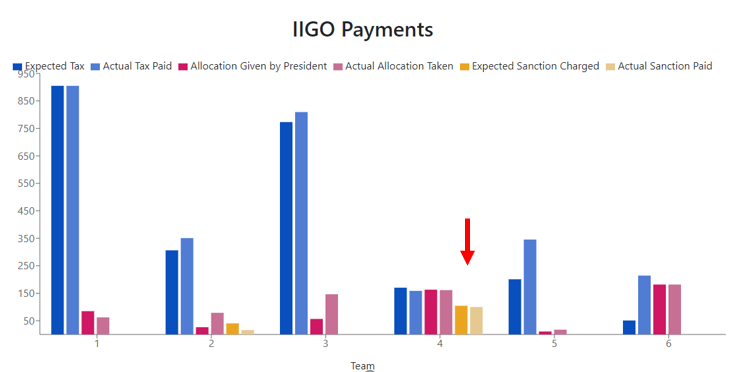
\includegraphics[scale=0.6]{12_team4_agentdesign/images/IIGOHO.PNG}
\caption{IIGO Payments For Honest Client Versus Other Teams.}
\label{fig:IIGOHO}
\end{figure}

\begin{figure}[H]
\centering
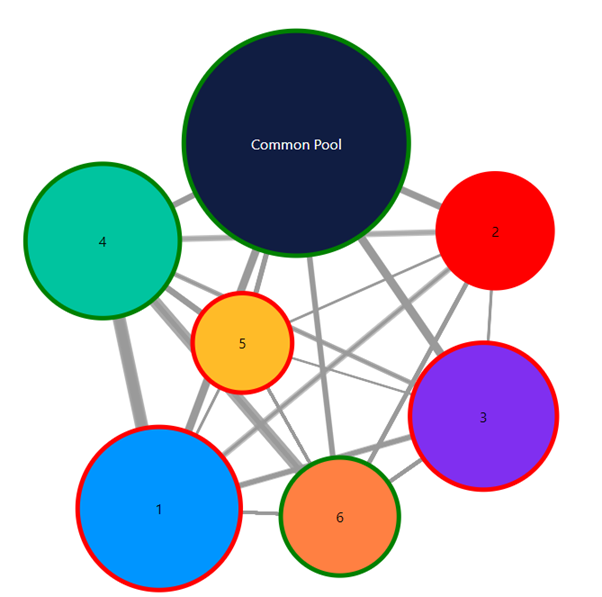
\includegraphics[scale=0.4]{12_team4_agentdesign/images/TransactionsHO.png}
\caption{Transactions For Honest Client Versus Other Teams.}
\label{fig:TransactionsHO}
\end{figure}
\begin{figure}[H]
\centering
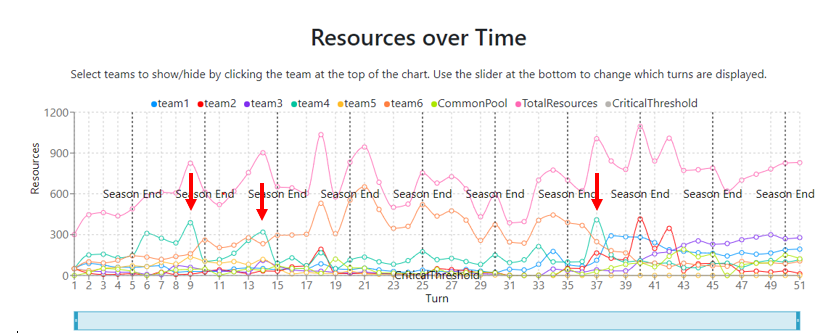
\includegraphics[scale=0.7]{12_team4_agentdesign/images/ResourcesHO.PNG}
\caption{Resources Plot For Honest Client Versus Other Teams.}
\label{fig:ResourcesHO}
\end{figure}

\subsubsection{Moderate Client} \label{moderateAO}
The \emph{moderate} client is configured specifically to start the game with an internal set of parameters that would allow it to score values as close as possible to thresholds in each decision making matrix calculation. The team opted for such a design choice in order to maximise the agent's response time to the environment, making it much more flexible than its two counterparts, who take a longer time to modify their strategy. As a Moderate client was simulated against other teams, the team noticed that it would perform very similarly as the Honest agent, as the other teams were always run on a "honest-like" configuration. Similarly, it would quickly turn its behaviour to dishonest when running against dishonest-like implementations of other teams' agents.

\subsubsection{Dishonest Client}
The \emph{dishonest} client, aptly named, is designed to take advantage of a large amount of common resources without collaborating with others and systematically abusing positions of power to gain economical advantages. The yielded results highlighted an interesting behaviour of the system and of other agents. As per design, the system can only incentivise avoidance of such radical and rogue behaviour, resulting in a complete dominance of the dishonest agent. The agent proceeds to appropriate of all resources from the common pool and mercilessly watch other islands die, as profiled in the Figure \ref{fig:ResourcesDO}. Eventually, unable to survive without the collective help to mitigate disasters, dishonest agent slowly meets its demise. The other agents do not reach a level of understanding of the game that allows them to comprehend the changes in game state, adapt to them, and mitigate them by enforcing more severe rules. It must also be said that the system itself does not allow any hard enforcement, making it impossible for other agents to counter-attack a fully dishonest and selfish strategy, which disregards sanctions and taxes. 

Given these findings, dishonesty might seem like a dominant strategy as the agent survives the longest, securing all resources for itself. However, the long term dilemma imposes that islands must collaborate to survive for long periods. The dominance of this strategy is further refuted by the simulations performed in subsection \ref{dishonestAD}.

\begin{figure}[H]
\centering
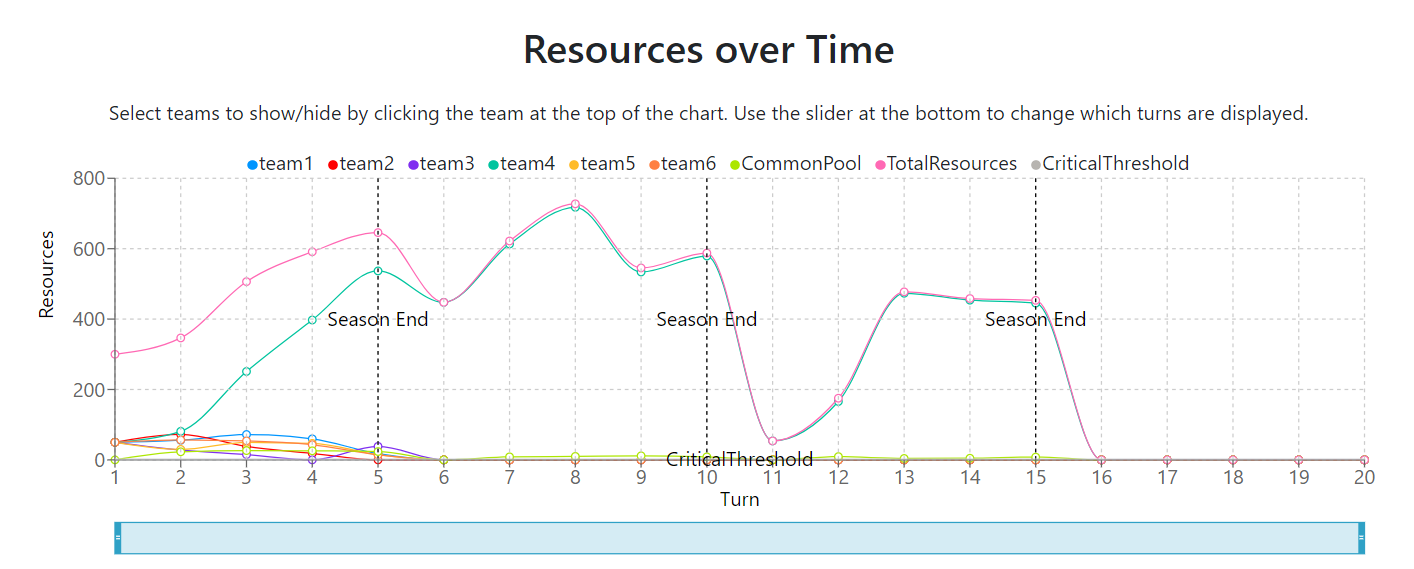
\includegraphics[scale=0.4]{12_team4_agentdesign/images/ResourcesDO.png}
\caption{Resources Plot For Dishonest Client Versus Other Teams.}
\label{fig:ResourcesDO}
\end{figure}

\subsection{Uni-Agent Simulations} \label{againstself}
There are observations to be made from simulating our agent against instances of itself. The main issue identified can be referred to as a \emph{lack of variety}, which encompasses the problem of populating the archipelago with islands that share the same "mindset"; therefore, approach dilemma from a unified perspective. This hypothesis was raised as an attempt to explain the poor results of uni-client simulations which have been observed not only when running team 4 agents against themselves.

In all uni-agent simulations, the common pool was initialised to 1,000 resources, so that the agents could have enough resources to initialise running IIGO sessions.

\subsubsection{Honest Agents Only}
Populating the game with only honest clients provided a starting environment where all clients in the game are inclined to obey to rules and contribute a lot to the common pool in collective efforts. From this standpoint it makes sense that clients would build strong relations of trust and retain a high opinion of each other, as they treat each other with a fair and collaborative personality. Therefore in the evolution of the game, no agent undertakes any radical change of personality as was the case when our honest client was placed against other teams in subsection \ref{honestAO}. The IIGO Payments histogram in Figure \ref{fig:IIGOHH} nicely shows how the islands do not break any rule throughout the entire run.

It also manifests a very predictable behaviour of each honest agent that is perfectly in line with their design, such as paying more taxes than requested and taking less allocations than granted. We identified this predictable behaviour as an example of \emph{lack of variety} that shows how agents with the same specification do not have strengths in all aspects of the system to survive in such a complex system that needs to be properly discovered and efficiently exploited.

\begin{figure}[H]
\centering
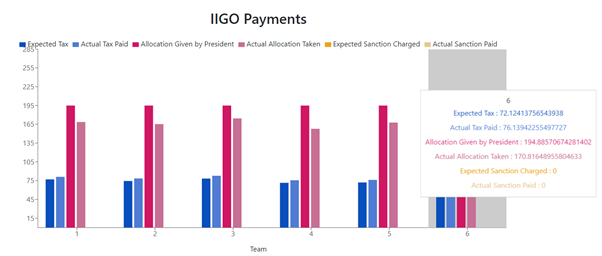
\includegraphics[scale=0.8]{12_team4_agentdesign/images/IIGOHH.png}
\caption{IIGO Payments For Honest Clients Only.}
\label{fig:IIGOHH}
\end{figure}

\subsubsection{Moderate Agents Only}
As presented in subsection \ref{moderateAO}, moderate agents are specifically designed to increase the variance in agent strategy. As a result, the \emph{lack of variety} issue should have been mitigated in a simulation where moderate agents face each other. After running the simulations, the clients have indeed acted far less predictably. Comparing Figure \ref{fig:IIGOMM} with the histogram plot shown in Figure \ref{fig:IIGOHH}, the breadth of a larger variety of game strategies can be observed. Namely, agent 2 and 3 show more dishonest traits, hence getting sanctions for performing illegal actions. Meanwhile, other clients take a more honest approach which replicates the ones observed by the honest clients. For other clients, like number 6, this honest strategy is less pronounced.

\begin{figure}[H]
\centering
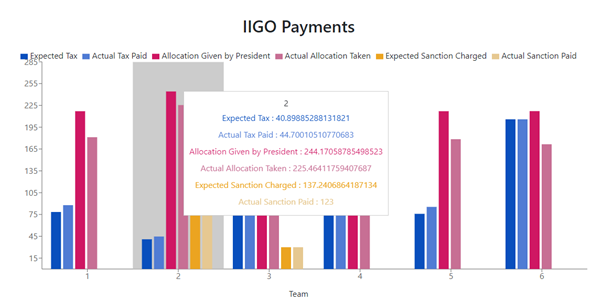
\includegraphics[scale=0.8]{12_team4_agentdesign/images/IIGOMM.png}
\caption{IIGO Payments For Moderate Clients Only.}
\label{fig:IIGOMM}
\end{figure}

Although the variance of agents strategy is significantly higher, clients still share the same underlying "mindset". This means that they define their whole personality using the same features, such as approaching tasks like foraging and power roles in the same way. Therefore, although the simulations ran show a slight improvement compared to "only honest" and "only dishonest" studies, they are far from producing a successful game like in multi-agent simulations. One of the main causes of this phenomenon was identified as the poor performance of actions that have been deliberately implemented in a simpler way in order to reduce the complexity of the agent. In particular, a foraging strategy in a well-performing multi-agent system may be to just replicate the foraging decision of the team that is economically strongest. However, in a uni-agent environment, this strategy  results in a group of agents mutually trusting their foraging strategy where nobody considers which one is actually the most profitable given the current circumstances.

Furthermore, features such as proposing rules is another good example of how lacking variety results in weaker archipelagos. This action enhances the ability of clients to adapt to the environment, crafting new rules as unexpected situations arise. If a client decides not to implement this feature in a multi-agent system, its effect on the adaptive capability of the archipelago will be almost fully mitigated by more complex clients that do perform such action.

\subsubsection{Dishonest Agents Only} \label{dishonestAD}
The last pure uni-agent simulation shows how dishonest clients face each other. This is, by far, the setting in which island longevity suffers the most as all clients start off the game with the intent to take advantage of the full resources with no compassion for others - demonstrating that with uncurbed dishonest agents, the system and agents cannot sustain the game. Runs in this environment feature one of the island who wins the race and empties the common pool, leaving other islands to die. The whole demise is made even faster by the total lack of collaboration among agents. Figure \ref{fig:ResourcesDD} demonstrates just how fast the archipelago is decimated. This comes as an additional proof of the fact that dishonesty cannot be considered a dominant strategy, as it doesn't perform better than all other strategies of the agent no matter what strategy the other agents choose. Indeed an honest or moderate client in such a setting would perform significantly better.
\begin{figure}[H]
\centering
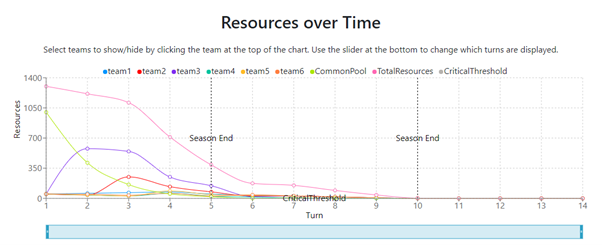
\includegraphics[scale=0.8]{12_team4_agentdesign/images/ResourcesDD.png}
\caption{Resources for Dishonest Clients Only.}
\label{fig:ResourcesDD}
\end{figure}

\subsubsection{Mixed Agents}
In an attempt to overcome the \emph{lack of variety} problem, simulations were run by instantiating two clients from each personality to promote variance. As demonstrated in Figure \ref{fig:IITOTransMA} via the “transactions” and “IITO” plots, the honest and moderate islands dominate in contributing to the community and share resources compared to the two dishonest clients “5 and 6”. Despite the clear difference in approaches from interaction plots, the game is still destined to finish early - failing to over come \emph{lack of variety}. This may be because agents are still sharing the same underlying “mindset” as they take decisions based on the same thresholds. They also are structured in the same way, so specific strategies like foraging or optional actions like proposing rules, if they are not implemented at all or just heavily relying on other clients making smart choices, will not work as well as in a more diverse environment.

\begin{figure}[H]
\centering
\begin{minipage}{.5\textwidth}
  \centering
  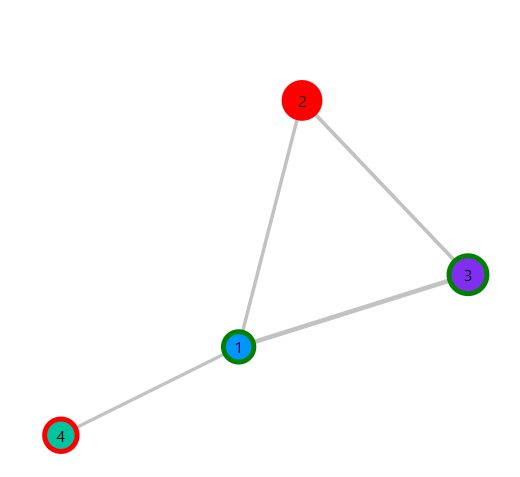
\includegraphics[width=.45\linewidth]{12_team4_agentdesign/images/IITOMA.png}
  IITO interactions
  %\captionof{IITO interactions}
\end{minipage}%
\begin{minipage}{.5\textwidth}
  \centering
  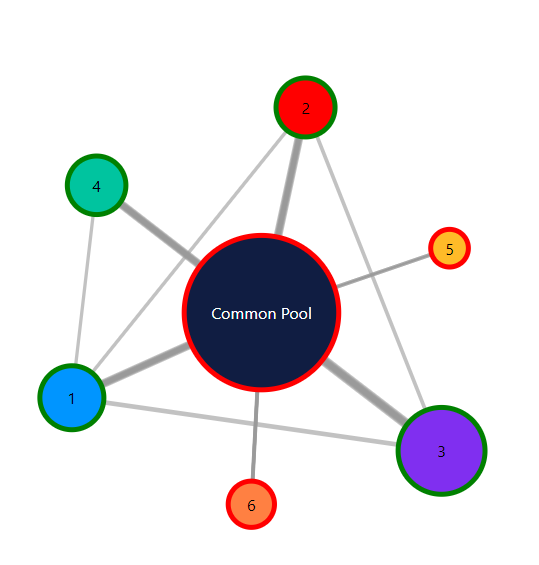
\includegraphics[width=.45\linewidth]{12_team4_agentdesign/images/TransactionsMA.png}
  Transactions
  %\captionof{Transactions}
\end{minipage}
  \label{fig:IITOTransMA}
  \caption{IITO interactions and transactions among mixed clients.}
\end{figure}


\subsection{Results Summary} \label{ResultSummary}
%Rudolfs suggestion on phrasing it as experts in the field allow all islands to thrive.%
\subsubsection{Lack of variety}
The \emph{lack of variety} problem was a reoccurring trend in all our uni-agent simulations. The question comes in when considering whether or not this trend was avoidable or not. Because our agents while having strengths in specific areas, had obvious weaknesses when it comes to rule proposal, putting the same agent up against each other resulted in a stalemate due to the lack of coverage of the game's functionalities. This could be a problem with agents that do not have a high level understanding of the whole game.

This begs the question on whether an optimal strategy would even exist on a game such as this if all participating agents have the same level of complexity. A possible solution to this may be to have a more advanced state machine, an agent design our team has considered on the developing stages. The core concept is that an agent can have a higher level of understanding of the situation the agent is put in. This indicates that in order to overcome the \emph{lack of variety} problem, it is not enough to have flexible thresholds and parameters, which are more tactical measures - the agent's design approach itself must be radically different at each state. This would require a lot of rewritten and well-partitioned code which was not sufficiently form-able in our limited time frame.

\subsubsection{Agent-institution interaction}

Evident by the behaviour of the dishonest agents, even with IIGO present, it is still possible to completely drain the common pool from any resources. As examined in the evaluation of IIGO, there are areas of power within IIGO which are not governed by institutional design. One of these is a lack of a Zone of Dignity, or similar solution, for the decisions on how much the agents should request in allocations and how much the President can allocate. In the current implementation there are no rules stating that the agent is not permitted to request resource amounts above some threshold. Moreover, there are no "guardrails" the President has to follow when allocating these resources. Thus a greedy agent, like the one we implemented, in combination with a generous President results in disastrous situations since the common pool stays permanently empty. There is no disaster mitigation and thus no source, besides presents, to reach for help in the case of critical financial status. Hence, a better approach to a dishonest agent in the current IIGO setting would be to keep all other agents minimally satisfied.

A more notable result is the one we see in regard to Ostrom's third principle. In the limited time our agent was developed in, it relies on the strategy of others for its own survival. The presence of other "expert" agents can aid in the survival of less developed ones. This is in line with the assumption behind opinion formation and voting. By allowing the agents to rely on the strategy of others, for example, relying on good disaster prediction algorithm from another agent, agents can disregard those aspects as long as they are satisfied with the work of the "experts". Similarly, our agent relies on the rule proposal of others to function. When there is a lack of experts and an agent lacks the ability to fill the institutional gaps in that field, that area of the institution collapses. This is also known as the problem students face when first coming to university and realising they have little expertise in cooking. 

One way to solve our agent's lack of expertise in rule proposal would be to make the agent spontaneously create rules or create all possible rules based on its understanding of the situation of the game. This requires effective collection of all useful information from the game, as well as successful interpretation of the information. In addition, the agent would need to predict the how rules interact with each other and what rules it desires in the short versus long term. A machine learning approach might be a good solution for this problem. The task is not trivial even for humans, however even sub-optimal solutions could benefit the agents ability to survive and interact with the institution.
    % \newcommand{\subsubsubsection}[1]{\paragraph{#1}\mbox{}\newline}
% \setcounter{secnumdepth}{4}
% \setcounter{tocdepth}{4}


%TODO: Please DO NOT RESOLVE the comments unless you are 100% sure everything related to the comment is resolved, as they can't be retrieved.
%TODO: VERY VERY IMPORTANT: talk to people in our group to make a decision on understanding of the "lack of variety"  that is shown in the comment on line 276 of this latex file. This will cause quite a few changes in the report but it is a very important concept to clarify to avoid burning ourselves. Read all the comments Mike made in the relevant sections first.
%TODO: VERY IMPORTANT: another potential self burn area. Clarify with Rudolfs about Ostrom's Principles after looking at all the comments Mike has made in that section.
%TODO: add in rule distance calculation explanation? It's kinda primitive though
%DONE: President by Andrzej, do talk about disaster prediction
%DONE I THINK: Toby to finish all foraging related stuff (IIFO and End of turn)
%DONE: add in the use of disaster prediction somewhere if we can?
%DONE: to finish IITO and gifting, sneak in disaster prediction if possible - This is done except for the disaster prediction part. Not sure how to add it though, but feel free if you have an idea how.
%TODO: clear up all the TODO's scattered around in this latex file.


\chapter{Team 4 Agent Design}   \label{chap:team4}
Given that our team invested a significant amount of time in ensuring feature richness and stability of the infrastructure, we were left with a short time-frame for our agent's implementation and design. Therefore, at times we had to make decisions that guaranteed canny usability, rather than sophistication. For some actions, our agent relies on other teams' agents with different strengths to perform well. 

\section{Agent overview}
An agent uses the interface that is defined in the infrastructure. In order to define custom behaviours for our agent, we override or extend the base agent (\texttt{baseclient.go}) functions which implement the defined interface. The team built the agent design upon a set of internal fields that aid the decision-making process for the actions it performs. Information to describe the agent's personality is recorded in a structure of internal parameters, namely \texttt{Greediness}, \texttt{Selfishness}, \texttt{Fairness}, \texttt{Collaboration} and \texttt{RiskTaking}, all of which have decimal values between 0 and 1. The agent stores observations, histories as well as other necessary information such as its trust in others. These internal fields will be discussed in more detail in the following dedicated sections. %TODO: add in evolutionary economic theory background for agent personality

An agent can be elected in one or more positions of power inside the IIGO session, and be able to perform the duties of the office. From an infrastructure standpoint, these actions are implemented as overridable functions in the same fashion as previously discussed for the base agent. Although the code was design to differentiate a commoner agent and roles in separate structs, they all share read and write access to the internal fields of each other through pointers. In other words, an agent is always a commoner agent, and a commoner agent can be elected one or more role(s) at the same time.

\section{Opinion formation -- Trust}
\label{sec:team4:trust}
Trust is the score $[0..1]$, which represents the agent's opinion towards fellow agents in the game. This metric helps it in making decisions throughout the game based on how trustworthy, helpful or friendly it believes other agents were. This generic opinion about an island is formed dynamically based on three recurring observations:
\begin{itemize}
    \item The gifts received from the island during the IITO sessions.
    \item The outcome of monitoring positions-of-power when conducted as a part of the accountability cycle.
    \item The evaluation of IIGO actions history, only available to the Judge. This is further explained in Section \ref{subsec:team4:judge}
\end{itemize}
Those observations allow the agent to quantitatively reason about both friendliness of other islands towards it, as well as how closely they follow the rules in play.

The average trust score is forced at a value of $0.5$. Such normalisation ensures that the trust is always balanced throughout the game. It prevents the inflation of trust in a scenario where several islands decide to exchange gifts with the agent. Furthermore, the number of resources gifted will be a deciding factor when updating the trust metrics.

Some decisions made by our agent can be altered based on the trust score towards certain islands. During elections, if the trust of an island is lower than a specified threshold, the agent will never cast its vote in favour of it. Similarly, if holding the role of Judge, it will choose not to act upon its power to pardon the island with a low trust score.

On the other hand, if the agent holds a good opinion about an island, it may choose to favour it by providing or even deciding to  pardon it from a sanction.


\section{IIGO}
\subsection{Commoner Agent} \label{commoneragent}
At the start of any IIGO, each (commoner) agent is prompted by the president to report how many resources it has. Our agent overrides its reporting behavior  to account for several internal factors, as further discussed in subsection \ref{reportresources}. The president uses this information to set a taxation amount according to each agent's self-report, notifying them of the tax demanded. Each (commoner) agent can later send a request for the specific amount of resources it aims to retrieve from the Common Pool (an allocation request) to the President. Upon receiving a response from the President on the actual amount that was granted, the agent is allowed to access the Common Pool. The actions concerning requesting and taking allocations are overridden, as part of the agent strategy. Due to a design decision, the action for taking allocations and paying tax does not happen within the IIGO session, it happens after all organisations are run, inside the \texttt{EndOfTurn} session.

\subsubsection{Report Resources} \label{reportresources}
When reporting its resources, our agent uses a weighted linear combination of some of its internal fields. The weighting of each parameter is defined as an array of real values called "importance" and stored in an \texttt{importance} vector. The linear combination outputs a scaling factor to divide to the actual resources our agent has, as shown in \eqref{linear_comb}, in order to compute an untruthful amount to report to the President. The parameters used are \texttt{greediness}, \texttt{selfishness}, \texttt{fairness}, \texttt{collaboration}, \texttt{riskTaking} and trust in the current president (all values are between 0 and 1). Some fields are associated with negative weights as they should logically negatively impact the scaling factor. The greater the absolute value of weight, the bigger impact it has on the scaling factor.

\begin{equation}\label{linear_comb}
    \begin{bmatrix}
        w_{1}& w_{2}& w_{3}& w_{4}& w_{5}& w_{6}
    \end{bmatrix}
    \cdot
    \begin{bmatrix}
    Greediness \\ 
    Selfishness \\ 
    Fairness \\ 
    Collaboration \\ 
    RiskTaking \\
    TrustScore_{President}
    \end{bmatrix}
    = Scaling\:Factor
\end{equation}

To decide when to lie, the scaling factor is first compared to a preset threshold. If the scaling factor is greater, then the amount of the needed resource is divided by 
\begin{equation}
    [1 + (Scaling\:Factor - Preset\:Threshold)]
\end{equation} 
This conditional statement makes sure that the scaling factor is not always applied, ensuring that our agent will lie on its resources only when deemed a good strategy.

\subsubsection{Paying Tax Contribution}
%write about this and the lying mechanics
The \texttt{GetTaxContribution()} function returns the amount an agent is paying in tax. Similarly to resource reporting, the tax amount is modified by a scaling factor applied only when greater than a preset threshold, as shown in the following equation: 
\begin{equation}
    [1 + (Scaling \: Factor - Preset \: Threshold)]
\end{equation}
Based on the preset weighting for internal parameters, this situation is likely to arise when the \texttt{Collaboration} of our agent is high. In addition, the scaling factor is not applied when the tax demanded is more than $\frac{1}{5}$ of the agent's resources. This prevents it from generously giving out most that it has.

\subsubsection{Requesting Allocation}\label{subsubsection:CommonPoolResourceRequest()}

The aforementioned action of requesting resources from the common pool is implemented in the function: \texttt{CommonPoolResourceRequest()}. When requesting an allocation, our agent first decides what it needs. When not in a critical state, the needed resources are usually a multiple of the basic needs, namely the cost of living plus the critical threshold. This amount is decided so that the agent always takes more from the Common Pool than their definite expenses in the next turn. If critical, the agent will ask for a bigger multiple of the basic needs. This design choice maps the following logical conclusion that the agent draws from the history of the game: if the a smaller multiple when made the agent critical, it must take more to invert the negative trend in resources. In order to avoid draining the Common Pool, our design enforces that what our island needs must not exceed the number of resources in the Common Pool divided by the number of agents alive. This is to avoid our agent selfishly monopolising the Common Pool resources.

\subsection{President}
\label{subsec:team4:president}
Our agent implements a budget-conscious and rule-obeying President. The main changes, compared to the basic implementation include taxation and resource allocation considerations.

\subsubsection{Tax distribution}
When deciding tax amounts for the different island, the President considers the following variables:
\begin{itemize}
    \item amount of resources in the common pool
    \item the financial status of the island
    \item predicted disaster time and magnitude.
\end{itemize}

The President will abstain from setting taxation for islands in a critical state or in a situation when the resources in the common pool can fully mitigate the predicted damage caused by the next disaster. 

Similarly, when the common pool cannot mitigate the next disaster, the President will set taxation for all non-critical island to bring the common pool back to the safe level. In this case, the taxation amount will be higher the sooner the disaster is predicted to occur.

\subsubsection{Common pool resource redistribution}
In order to fairly redistribute the resources placed in the common pool, the President primarily considers the financial status of an island. In other words, the priority in access to the common pool is given to islands in the critical state. 

To ensure the largest possible satisfaction within the archipelago, the islands with smaller requests are given priority. This decision ensures that the highest possible number of agents will be satisfied with their allocation.

The President is also reluctant to allow any resource allocations if the disaster is predicted to occur soon. This, combined with the tax policy, ensures lower damages to the archipelago in the case of disaster.


\subsection{Judge}
\label{subsec:team4:judge}
The Judge implementation provided by our agent can be described as \emph{honest, but curious}. In other words, it follows the rules currently in play, and follows its obligations, however, it extracts the information exclusive to the Judge to reason about other agents in the game. An example of such actions is explained in greater detail below in this Section.

The judiciary functions overloaded from the \texttt{basejudge} implementation are:
\begin{itemize}
    \item \texttt{InspectHistory}, which examines rule violations of all the agents.
    \item \texttt{GetPardonedIslands}, which considers reducing the sanctions for some agents at judges discretion.
    \item \texttt{CallPresidentElection}, which initialises \emph{transfer-of-power} of the executive branch.
\end{itemize}
An explanation of the implementation of those functions is presented below.

\subsubsection{IIGO history inspection}
\label{subsubsec:team4:judge:inspect_history}
In the basic implementation, a history of IIGO actions of all the agents is passed to the Judge for inspection, which could become grounds for introducing economic sanctions for non-rule-obeying players. 

Judge truthfully evaluates and reports the rule violations for each of the agents, just as the \texttt{basejudge}. However, it also extracts and saves the information about the private resource pools of all the agents, taxes they were expected to pay, as well as the actual amount paid to the common pool. Additionally, it stores the \texttt{LawfulnessRatio} of each agent, which is defined as:


\begin{equation}
    lawfulness_{i} = \frac{number\:of\:rules\:obeyed\:by\:the\:agent_{i}}{total\:number\:of\:rules\:inspected\:by\:the\:judge\:for\:agent_{i}}
\end{equation}

where $agent_{i}$ denotes the $i^{th}$ agent in the game.  

The \texttt{LawfulnessRatio} is then used to update our agents' trust towards other islands, thus influencing decisions in different parts of the game. 

\subsubsection{Consideration of pardons}
Compared to the \texttt{basejudge}, which does not grant any pardons and requires islands to pay economic sanctions in full, our implementation of the Judge allows for the pardoning of certain islands. We consider three parameters when deciding whether and the island could be pardoned:

\begin{enumerate}
    \item The severity of the sanction - only sanctions lower than specified severity level can be considered to be pardoned. This ensures that our Judge never pardons an island, who notoriously breaks the rules of the game and gets sanctioned for it.
    \item Time served on the sanction - the Judge will only remove the sanction if at least the specified number of turns has been served by the island. This still allows us to have a punishment for not obeying the rules but also ensures that an island can begin to contribute again earlier.
    \item Trust towards the island sanctioned - only islands, which are considered trustworthy by our agent can be pardoned. The threshold is tuned by an internal parameter of our agent.
\end{enumerate}

An island can be pardoned by our implementation of Judge only if they meet all three requirements presented above. 


\subsubsection{Presidential elections}
The \texttt{basejudge} implementation called an election every three turns, no matter how long the presidential term was. Our Judge implementation improves on that by calling an election only under two conditions:
\begin{enumerate}
    \item The term of the president has ended.
    \item The president did not fulfil its obligations and was dishonest while holding the executive office. It is decided based on the monitoring results coming from the accountability cycle.
\end{enumerate}

This implementation could be further improved to facilitate the \emph{trust} metrics, explained in Section~\ref{sec:team4:trust}. An example of such an improvement would be allowing the president to hold the office longer than its turn if he is most trustworthy according to our internal \emph{trust} metrics.

\subsection{Speaker}
Given the Speaker's role of deciding agendas and announcing the results of the voting, the only viable customisation option in making our custom Speaker seemed to be implementing corruption - in other words, rigging voting results. Other than the obvious reason of avoiding the risk of getting sanctions, we decided against implementing this function into the Speaker's role because in an actual governmental environment, while misprints have occurred and on occasion shaped past history, announcing false results are a very noticeable and easily rectifiable offense. This would be in the disinterest of either honest or dishonest agents. On this note and the following point, it could be said that our Speaker implementation can be described as \emph{honorable and efficient}.

\subsubsection{Action prioritisation}

Our Speaker implementation builds upon the \texttt{baseSpeaker} on a key point: partitioning of budget. The Speaker prioritises the proper running of IIGO in the case of a low budget situation by prioritising its actions according to the rules in play, reflecting the priorities decided by the archipelago. This is done not by changing the actual running order of IIGO (which would require altering the orchestration) but rather enabling/disabling certain actions based on their priorities and cost. Prioritising actions where rules are in play would stop the speaker from performing non-moderated actions instead of actions relating to rules that are still in play. This function is crucial due to the following reasons:
\begin{itemize}
    \item Not performing monitored actions will result in sanctions, harming the agent's resource pool.
    \item The rules are a representation of the archipelago's expectations, thus not following said priorities is a sign of incompetence - damaging the agent's reputation.
\end{itemize}
Since these reasons are applicable regardless of honesty, these mechanics are always implemented regardless of the chosen personality type.

\section{IIFO}\label{sec:team4:IIFO}
%I recommend that we write in the order of function execution order. (the end of turn functions that are related to IIFO should be written inside the EndOfTurn section)Only mention the functions that are worth mentioning. For execution order check the ./doc/EXECUTION_ORDER.md file in the SOMAS repo -- Mike

\subsection{Making Disaster Prediction}
The agent makes predictions about future disasters by getting the mean coordinates, magnitude and number of turns per disaster (i.e. $\frac{1}{freq}$) from the previous disasters. It then computes a \texttt{confidence} score based on these mean values. The \texttt{confidence} score has a range between 0\% and 100\%. The sum of square of difference between the actual value and the mean value for each of the 4 prediction values types(coordinate x, coordinate y, magnitude and turns) is calculated as below:
\begin{equation}
    total = \sum_{i=1}^{len(past\_disasters)}(Value_i - Mean_i)^2
\end{equation}

The above is done for each of the 4 prediction values types. This returns a measurement of the distance between the predicted value (mean value) and the corresponding past disasters' values. The computed sum of square of difference (a measure of distance) is normalised with a max distance (see equations \ref{max_distance:1} to \ref{max_distance:3}) for each of the 4 value types, 100\% minus this percentage value is the \texttt{confidence} score. The \texttt{confidence} score for the prediction is the average of the 4 \texttt{confidence} scores.

Note that the Central Limit Theorem can be applied in this calculations since we assume different disasters are independent. Namely, the higher the distance between a prediction and samples, the less likely it is for this prediction to be true. And with the CLT assumption, the underlying random variables of the value types (uniform RV for coordinates, geometric RV for both magnitude and turns) do not matter. The calculation of the unique preset threshold is below:
\begin{equation}\label{max_distance:1}
    distance_1 = \sum_{i=1}^{len(past\_disasters)}(ValueMax - Mean_i)^2
\end{equation}
\begin{equation}\label{max_distance:2}
    distance_2 = \sum_{i=1}^{len(past\_disasters)}(ValueMin - Mean_i)^2
\end{equation}
\begin{equation}\label{max_distance:3}
    max\: distance = max (distance_1, distance_2)
\end{equation}

By doing the above unique threshold calculation for each value type, we are setting the predicted values out of bounds to have confidence 0\%. (Note: ValueMax and ValueMin are set in game config)

\subsubsection{Making prediction based on other agents' predictions}
Our agent then receives prediction information from all other agent that sent their information to us. A weighted average (based on trust) of these prediction values are calculated to form our final prediction values.

%Theoretically, We would use  a normal distribution to approximate the sampling distribution of the disaster random variable, which is assumed to be independent across turns, justified by the Central Limit Theorem. And by feeding  calculation approximated to be 


% Foraging functions %
\subsection{Sharing foraging information} \label{sec:team4:IIFO:forage}
IIFO also contains the ability to communicate about the foraging information. As we will go further into in Section~\ref{sec:team4:forage},
we choose to overload both MakeForageInfo and ReceiveForageInfo. In the receive function, we store the received values to a map to be used later when making a decision on which foraging method to go for. 

As we use the foraging information from other teams, our island will also communicate our results to the others. However, we only share with islands that shared with us in the previous round, as well as the island that we trust. Our island is completely truthful for this part and will always report which foraging method we went for, as well as how many resources it generated.

\subsection{IITO}
%(put and modify this to fit it somewhere in this section) If our agent is not in a critical state, it requests extra resources in addition to its own wanted resources in an intention to gift to other agents to earn their trust. If this allocation request is approved by the President, it proceeds with the gifting. These gifted resources are given on top of the normal gifts if there are any.
% some rough comments about IITO from Fabio: gifting pool is the key concept. same as president for allocation. Prioritise agents that are critical. Look at our selfishness and current resources. Help critical first(full amount no matter the trust). If not critical, only gift if trust > 0.5
In IITO we handle the process of sending, receiving, and requesting gifts.
Our island has an internal wealth goal which is calculated using our internal greediness and selflessness parameters. If our private pool is smaller than our wealth goal we ask for gifts from the other islands. The amount we ask for is related to the difference between the private pool and wealth goal. If we are in a critical state, however, we ask every island for two times the resources we estimate to be a safe resource level in the hope that at least one island will support us. 

When an island requests a gift from us we first check how many resources we can spare. This is once again calculated by taking the difference between the private pool and the wealth goal. We also look into its trustworthiness. If the island is critical, we prioritise that island. After that, we only return the gift relative to their trustworthiness. 
In addition, when we request allocation in IIGO, we request a bit extra which we gift to other islands in the hope that it will increase our reputation. This is only done if the president permits us to take the extra resources. 


 

\section{End of Turn}
\subsection{Taking Allocation}
This RequestAllocation() function for taking allocation from the Common Pool. After running all of the organisation sessions, the agent then calculates what it wants based on what it needs, and takes what it wants from the Common Pool. A scaling factor is calculated using a linear combination of weights and internal fields. When the scaling factor is above a preset threshold, it is applied similar to in Section~\ref{subsubsection:CommonPoolResourceRequest()}.  %talking about scaling factor calculation briefly, the detailed explanation is already done in ResourceReport. %%We use a linear combination of some of the agent's internal fields, and weights (put inside an \texttt{importance} vector) we set for each of the chosen internal fields to obtain a scaling factor to multiply the needed resources with. The parameters used are \texttt{greediness}, \texttt{selfishness}, \texttt{fairness}, \texttt{collaboration}, \texttt{riskTaking} and trust in the current president (all values are between 0 and 1). The weights have real values. For this particular function, we set the weights to be $5, 5, -5, -5, 1, 5$ respectively. The fields with negative weights negatively impact the scaling factor and vice versa. We deem riskTaking less important than other fields in the calculation of this function's scaling factor. The scaling factor is then compared to a preset threshold. If the scaling factor is greater, then the needed resources amount is multiplied by 1 plus the difference between the scaling factor and the preset threshold. The threshold is there to make sure that the scaling factor is not applied all the time, as we don't want our agent to take more than what it needs all the time.

\subsection{Forage} \label{sec:team4:forage}
As mentioned at the start of the chapter, due to the interest of time, our foraging strategy relies on other islands to make intelligent decisions about the foraging strategy. In short, rather than looking at the game configurations to try to intelligently figure out which method to go for and how many resources to generate, we look at other teams' return ratios to decide for ourselves. As will be discovered in the simulation section (\ref{sec:team4:simulation}), our foraging strategy works very well against the other islands created by the other teams, but not so well when we simulate six of our own islands.  

Our foraging strategy is split into two sections. Managing foraging communications is stored inside \texttt{IIFO.go} and our foraging decisions are stored inside \texttt{Foraging.go}.

As mentioned in Section~\ref{sec:team4:IIFO:forage}, 
the foraging is split into two parts, decision, and return. In the return, we store the results we receive into an array so that we can later use them in the decision making. This is also what we do inside IIFO when we receive the foraging results from the other teams. 

To decide whether to go fishing or to hunt deer the island looks at both its return history as well as looking at the return results received from the other teams. Our island does this is by calculating the return ratio of each island over the past three turns as well as our own. These ratios are then compounded into two separate values, the compounded ratio for deer hunting and the compounded ratio for fishing.  We then pick the foraging method that has the greatest compound ratio. 

How the island chooses to share its foraging results with other islands was described earlier in Section~\ref{sec:team4:IIFO:forage}. 


\section{Simulation}\label{sec:team4:simulation}


\subsection{Introduction}
Three different initial personality configurations were defined -
\emph{honest} , \emph{moderate} and \emph{dishonest} - in order to simulate how internal parameters would impact the agent's performance and interaction with the other teams.
These agents are designed to adapt their decision-making processes throughout the game, and each of these different personalities drew interesting hypotheses and observations about how a single agent would affect other agents and the system as a whole. This will be further discussed in Section~\ref{ResultSummary}. 

%TODO: add in evolutionary economic theory background for agent personality if we can explain it, it's a really good thing to add


The team decided to test both the interactions in the archipelago when populated by our clients with different personalities and the default clients developed by other teams (discussed in Section~\ref{againstothers} \nameref{againstothers}) as well as the interactions when only populated by instances of our client (discussed in Section~\ref{againstself} \nameref{againstself}). These simulation efforts have been made to investigate the effectiveness of the agent's strategy, the system's response to the lack of strategy variance, as well as the ability of the agents to react to this issue.

\subsection{Multi-agent simulations} \label{againstothers}
\subsubsection{Honest Client} \label{honestAO}
The \emph{honest} client has been carefully designed as an agent who would start the game complying to rules, offering help when possible and contributing to the common pool with more taxes when the agent is in abundant wealth. However, the personality of the agent adapts to the environment as it self-organises its strategy based on fellow agents. An irrefutable sign of great flexibility of this agent configuration is the presence of sanctions in its IIGO Report as shown in Figure~\ref{fig:IIGOHO}. The figure testifies that the agent adopts a change in strategy, occasionally breaking the rules. It still maintains a fair and collaborative approach throughout the whole game, getting involved in transactions during the IITO (Figure~\ref{fig:TransactionsHO}) and contributing to the common pool. 

As shown in the Resources Plot in Figure~\ref{fig:ResourcesHO} , where the agent is represented by the cyan curve, more than once there is a peak in resources that steeply decreases on the following turn. This happens because the agent is generously providing gifts to the agents in need and sometimes is also paying slightly more taxes into the common pool than required. From a design standpoint the team opted for an implementation that would prioritise gifts over over-contributions to the common pool. This decision comes from the consideration that a dishonest agent would counter our efforts in distributing resources to fellow agents. Therefore, prioritising gifting avoids this problem by allowing our agent to deliberately allocate its resources surplus to other islands. The agent acts even more magnanimously with islands in a critical state. This behaviour is clearly noticeable in disaster recovery.
\begin{figure}[H]
\centering
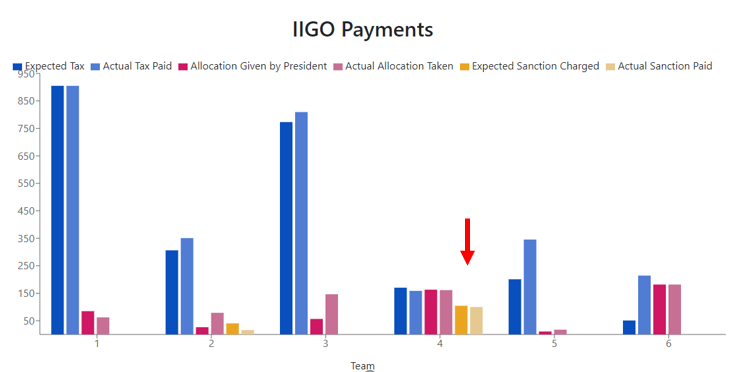
\includegraphics[scale=0.6]{12_team4_agentdesign/images/IIGOHO.PNG}
\caption{IIGO Payments For Honest Client Versus Other Teams.}
\label{fig:IIGOHO}
\end{figure}

\begin{figure}[H]
\centering
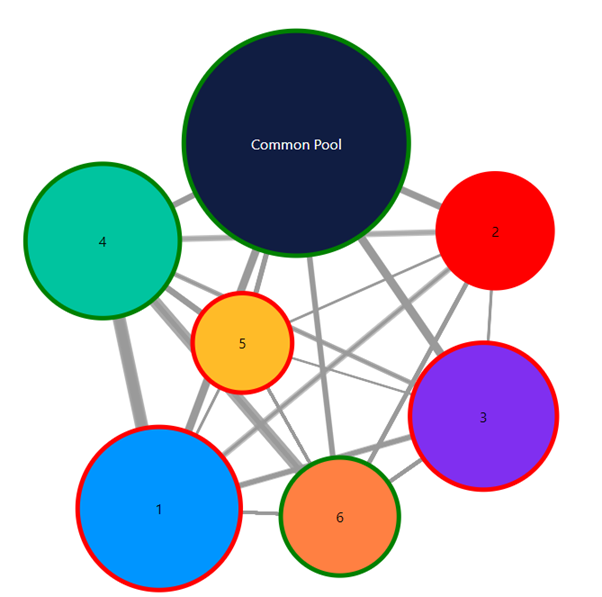
\includegraphics[scale=0.4]{12_team4_agentdesign/images/TransactionsHO.png}
\caption{Transactions For Honest Client Versus Other Teams.}
\label{fig:TransactionsHO}
\end{figure}
\begin{figure}[H]
\centering
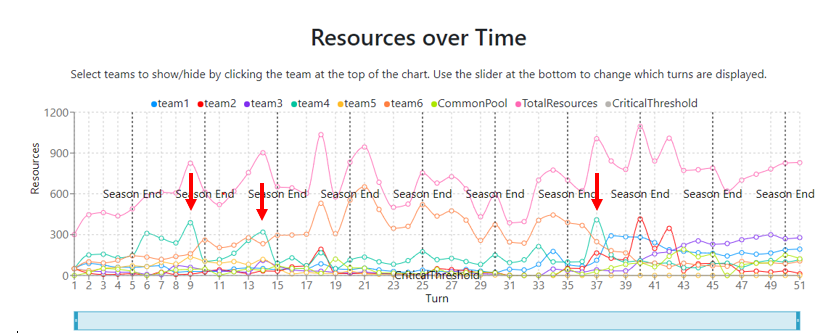
\includegraphics[scale=0.7]{12_team4_agentdesign/images/ResourcesHO.PNG}
\caption{Resources Plot For Honest Client Versus Other Teams.}
\label{fig:ResourcesHO}
\end{figure}

\subsubsection{Moderate Client} \label{moderateAO}
The \emph{moderate} client is configured specifically to start the game with an internal set of parameters that would allow it to score values as close as possible to thresholds in each decision making matrix calculation. The team opted for such a design choice in order to maximise the agent's response time to the environment, making it much more flexible than its two counterparts, who take a longer time to modify their strategy. As a Moderate client was simulated against other teams, the team noticed that it would perform very similarly as the Honest agent, as the other teams were always run on a "honest-like" configuration. Similarly, it would quickly turn its behaviour to dishonest when running against dishonest-like implementations of other teams' agents.

\subsubsection{Dishonest Client}
The \emph{dishonest} client, aptly named, is designed to take advantage of a large amount of common resources without collaborating with others and systematically abusing positions of power to gain economical advantages. The yielded results highlighted an interesting behaviour of the system and of other agents. As per design, the system can only incentivise avoidance of such radical and rogue behaviour, resulting in a complete dominance of the dishonest agent. The agent proceeds to appropriate of all resources from the common pool and mercilessly watch other islands die, as profiled in the Figure \ref{fig:ResourcesDO}. Eventually, unable to survive without the collective help to mitigate disasters, dishonest agent slowly meets its demise. The other agents do not reach a level of understanding of the game that allows them to comprehend the changes in game state, adapt to them, and mitigate them by enforcing more severe rules. It must also be said that the system itself does not allow any hard enforcement, making it impossible for other agents to counter-attack a fully dishonest and selfish strategy, which disregards sanctions and taxes. 

Given these findings, dishonesty might seem like a dominant strategy as the agent survives the longest, securing all resources for itself. However, the long term dilemma imposes that islands must collaborate to survive for long periods. The dominance of this strategy is further refuted by the simulations performed in subsection \ref{dishonestAD}.

\begin{figure}[H]
\centering
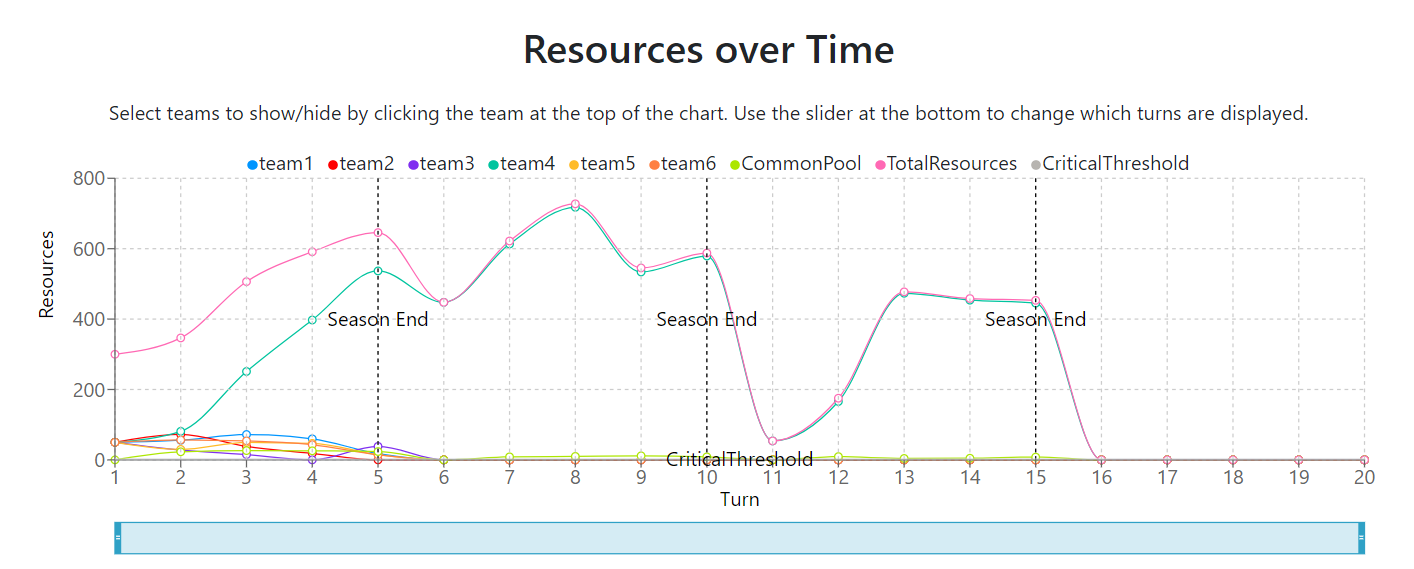
\includegraphics[scale=0.4]{12_team4_agentdesign/images/ResourcesDO.png}
\caption{Resources Plot For Dishonest Client Versus Other Teams.}
\label{fig:ResourcesDO}
\end{figure}

\subsection{Uni-Agent Simulations} \label{againstself}
There are observations to be made from simulating our agent against instances of itself. The main issue identified can be referred to as a \emph{lack of variety}, which encompasses the problem of populating the archipelago with islands that share the same "mindset"; therefore, approach dilemma from a unified perspective. This hypothesis was raised as an attempt to explain the poor results of uni-client simulations which have been observed not only when running team 4 agents against themselves.

In all uni-agent simulations, the common pool was initialised to 1,000 resources, so that the agents could have enough resources to initialise running IIGO sessions.

\subsubsection{Honest Agents Only}
Populating the game with only honest clients provided a starting environment where all clients in the game are inclined to obey to rules and contribute a lot to the common pool in collective efforts. From this standpoint it makes sense that clients would build strong relations of trust and retain a high opinion of each other, as they treat each other with a fair and collaborative personality. Therefore in the evolution of the game, no agent undertakes any radical change of personality as was the case when our honest client was placed against other teams in subsection \ref{honestAO}. The IIGO Payments histogram in Figure \ref{fig:IIGOHH} nicely shows how the islands do not break any rule throughout the entire run.

It also manifests a very predictable behaviour of each honest agent that is perfectly in line with their design, such as paying more taxes than requested and taking less allocations than granted. We identified this predictable behaviour as an example of \emph{lack of variety} that shows how agents with the same specification do not have strengths in all aspects of the system to survive in such a complex system that needs to be properly discovered and efficiently exploited.

\begin{figure}[H]
\centering
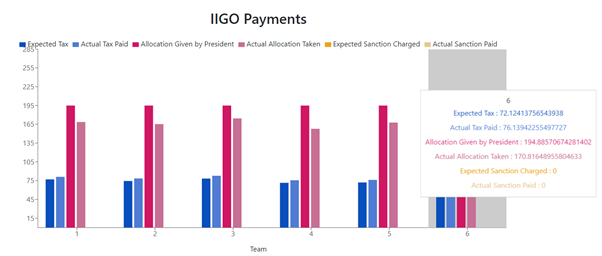
\includegraphics[scale=0.8]{12_team4_agentdesign/images/IIGOHH.png}
\caption{IIGO Payments For Honest Clients Only.}
\label{fig:IIGOHH}
\end{figure}

\subsubsection{Moderate Agents Only}
As presented in subsection \ref{moderateAO}, moderate agents are specifically designed to increase the variance in agent strategy. As a result, the \emph{lack of variety} issue should have been mitigated in a simulation where moderate agents face each other. After running the simulations, the clients have indeed acted far less predictably. Comparing Figure \ref{fig:IIGOMM} with the histogram plot shown in Figure \ref{fig:IIGOHH}, the breadth of a larger variety of game strategies can be observed. Namely, agent 2 and 3 show more dishonest traits, hence getting sanctions for performing illegal actions. Meanwhile, other clients take a more honest approach which replicates the ones observed by the honest clients. For other clients, like number 6, this honest strategy is less pronounced.

\begin{figure}[H]
\centering
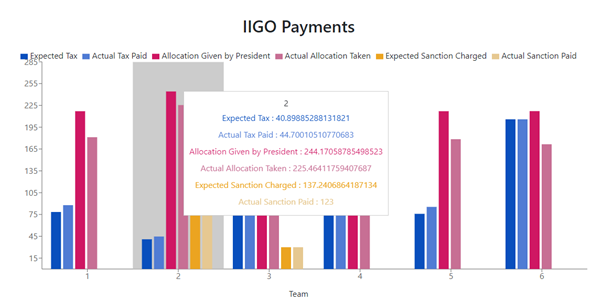
\includegraphics[scale=0.8]{12_team4_agentdesign/images/IIGOMM.png}
\caption{IIGO Payments For Moderate Clients Only.}
\label{fig:IIGOMM}
\end{figure}

Although the variance of agents strategy is significantly higher, clients still share the same underlying "mindset". This means that they define their whole personality using the same features, such as approaching tasks like foraging and power roles in the same way. Therefore, although the simulations ran show a slight improvement compared to "only honest" and "only dishonest" studies, they are far from producing a successful game like in multi-agent simulations. One of the main causes of this phenomenon was identified as the poor performance of actions that have been deliberately implemented in a simpler way in order to reduce the complexity of the agent. In particular, a foraging strategy in a well-performing multi-agent system may be to just replicate the foraging decision of the team that is economically strongest. However, in a uni-agent environment, this strategy  results in a group of agents mutually trusting their foraging strategy where nobody considers which one is actually the most profitable given the current circumstances.

Furthermore, features such as proposing rules is another good example of how lacking variety results in weaker archipelagos. This action enhances the ability of clients to adapt to the environment, crafting new rules as unexpected situations arise. If a client decides not to implement this feature in a multi-agent system, its effect on the adaptive capability of the archipelago will be almost fully mitigated by more complex clients that do perform such action.

\subsubsection{Dishonest Agents Only} \label{dishonestAD}
The last pure uni-agent simulation shows how dishonest clients face each other. This is, by far, the setting in which island longevity suffers the most as all clients start off the game with the intent to take advantage of the full resources with no compassion for others - demonstrating that with uncurbed dishonest agents, the system and agents cannot sustain the game. Runs in this environment feature one of the island who wins the race and empties the common pool, leaving other islands to die. The whole demise is made even faster by the total lack of collaboration among agents. Figure \ref{fig:ResourcesDD} demonstrates just how fast the archipelago is decimated. This comes as an additional proof of the fact that dishonesty cannot be considered a dominant strategy, as it doesn't perform better than all other strategies of the agent no matter what strategy the other agents choose. Indeed an honest or moderate client in such a setting would perform significantly better.
\begin{figure}[H]
\centering
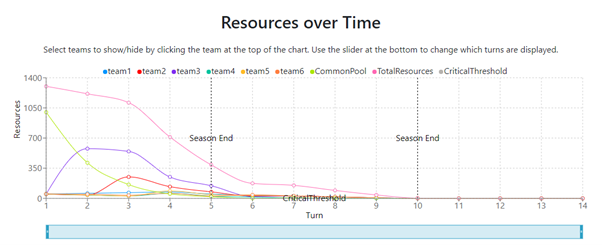
\includegraphics[scale=0.8]{12_team4_agentdesign/images/ResourcesDD.png}
\caption{Resources for Dishonest Clients Only.}
\label{fig:ResourcesDD}
\end{figure}

\subsubsection{Mixed Agents}
In an attempt to overcome the \emph{lack of variety} problem, simulations were run by instantiating two clients from each personality to promote variance. As demonstrated in Figure \ref{fig:IITOTransMA} via the “transactions” and “IITO” plots, the honest and moderate islands dominate in contributing to the community and share resources compared to the two dishonest clients “5 and 6”. Despite the clear difference in approaches from interaction plots, the game is still destined to finish early - failing to over come \emph{lack of variety}. This may be because agents are still sharing the same underlying “mindset” as they take decisions based on the same thresholds. They also are structured in the same way, so specific strategies like foraging or optional actions like proposing rules, if they are not implemented at all or just heavily relying on other clients making smart choices, will not work as well as in a more diverse environment.

\begin{figure}[H]
\centering
\begin{minipage}{.5\textwidth}
  \centering
  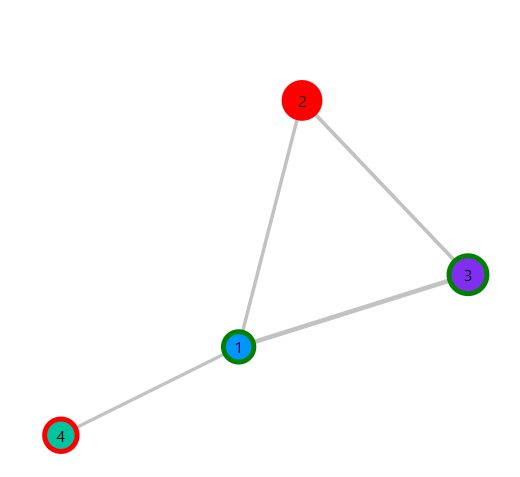
\includegraphics[width=.45\linewidth]{12_team4_agentdesign/images/IITOMA.png}
  IITO interactions
  %\captionof{IITO interactions}
\end{minipage}%
\begin{minipage}{.5\textwidth}
  \centering
  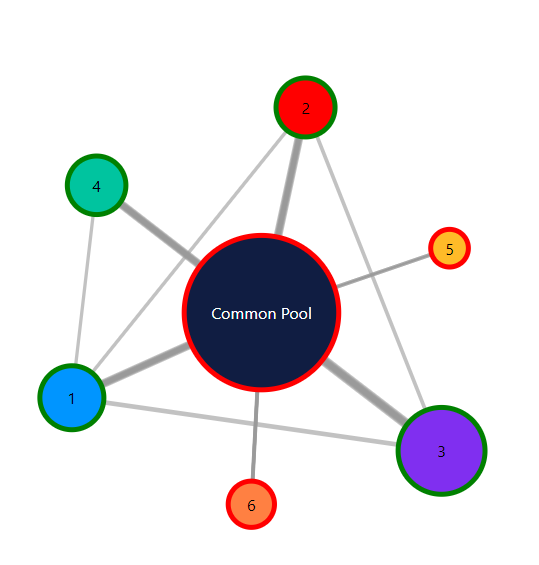
\includegraphics[width=.45\linewidth]{12_team4_agentdesign/images/TransactionsMA.png}
  Transactions
  %\captionof{Transactions}
\end{minipage}
  \label{fig:IITOTransMA}
  \caption{IITO interactions and transactions among mixed clients.}
\end{figure}


\subsection{Results Summary} \label{ResultSummary}
%Rudolfs suggestion on phrasing it as experts in the field allow all islands to thrive.%
\subsubsection{Lack of variety}
The \emph{lack of variety} problem was a reoccurring trend in all our uni-agent simulations. The question comes in when considering whether or not this trend was avoidable or not. Because our agents while having strengths in specific areas, had obvious weaknesses when it comes to rule proposal, putting the same agent up against each other resulted in a stalemate due to the lack of coverage of the game's functionalities. This could be a problem with agents that do not have a high level understanding of the whole game.

This begs the question on whether an optimal strategy would even exist on a game such as this if all participating agents have the same level of complexity. A possible solution to this may be to have a more advanced state machine, an agent design our team has considered on the developing stages. The core concept is that an agent can have a higher level of understanding of the situation the agent is put in. This indicates that in order to overcome the \emph{lack of variety} problem, it is not enough to have flexible thresholds and parameters, which are more tactical measures - the agent's design approach itself must be radically different at each state. This would require a lot of rewritten and well-partitioned code which was not sufficiently form-able in our limited time frame.

\subsubsection{Agent-institution interaction}

Evident by the behaviour of the dishonest agents, even with IIGO present, it is still possible to completely drain the common pool from any resources. As examined in the evaluation of IIGO, there are areas of power within IIGO which are not governed by institutional design. One of these is a lack of a Zone of Dignity, or similar solution, for the decisions on how much the agents should request in allocations and how much the President can allocate. In the current implementation there are no rules stating that the agent is not permitted to request resource amounts above some threshold. Moreover, there are no "guardrails" the President has to follow when allocating these resources. Thus a greedy agent, like the one we implemented, in combination with a generous President results in disastrous situations since the common pool stays permanently empty. There is no disaster mitigation and thus no source, besides presents, to reach for help in the case of critical financial status. Hence, a better approach to a dishonest agent in the current IIGO setting would be to keep all other agents minimally satisfied.

A more notable result is the one we see in regard to Ostrom's third principle. In the limited time our agent was developed in, it relies on the strategy of others for its own survival. The presence of other "expert" agents can aid in the survival of less developed ones. This is in line with the assumption behind opinion formation and voting. By allowing the agents to rely on the strategy of others, for example, relying on good disaster prediction algorithm from another agent, agents can disregard those aspects as long as they are satisfied with the work of the "experts". Similarly, our agent relies on the rule proposal of others to function. When there is a lack of experts and an agent lacks the ability to fill the institutional gaps in that field, that area of the institution collapses. This is also known as the problem students face when first coming to university and realising they have little expertise in cooking. 

One way to solve our agent's lack of expertise in rule proposal would be to make the agent spontaneously create rules or create all possible rules based on its understanding of the situation of the game. This requires effective collection of all useful information from the game, as well as successful interpretation of the information. In addition, the agent would need to predict the how rules interact with each other and what rules it desires in the short versus long term. A machine learning approach might be a good solution for this problem. The task is not trivial even for humans, however even sub-optimal solutions could benefit the agents ability to survive and interact with the institution.
    \chapter{Team 5 Agent Design}
\section{Game Specification}
Our agent represents an island that exists in the Archipelago where it interacts and collaborates with other islands (agents). All agents interact with a Common Pool of resources which is primarily used to facilitate governmental procedures and mitigate natural disasters that may occur (long-term collective risk dilemma). As a result of the short-term collective risk dilemma, there is not enough resources to satisfy all of agents but only enough to satisfice \textit{some} of them. According to \textit{Self-Organizing Multi-Agent Systems} by Pitts, satisfy means having all agent's needs taken care of. On the other hand, satisfice means only the basic needs/minimum requirements have been met. In this economy of scarcity, it may be sufficient that the agent's needs are satisficed. Each island presumably will have the objective of maximising its individual utility which requires collaboration with other islands.

In our implementation, the levels of resources held by our agent are divided into 'wealth tiers' which influence our agent's decision making strategies. Our interactions with other agents are driven by our \texttt{opinion} of them which evolves over time in the game. In every round, our agent computes its current wealth status and updates its opinion of others based on various factors explored below.

\subsection{Wealth Tiers}
We have defined four different wealth tiers and the respective thresholds to represent the status of the agent according to its current resources. The wealth tiers are defined as follows:
\begin{enumerate}
    \item \texttt{dying}: critical status. 
    \item \texttt{imperialStudent}: lower class (<30\% of starting resources).
    \item \texttt{middleClass}: middle class (<95\% of starting resources).
    \item \texttt{jeffBezos}: upper class (<200\% of starting resources).
\end{enumerate}

\subsection{Opinion Formation}
\label{subsec: opinion-formation}
\subsubsection{Design}
An opinion of other islands is our agent's general perception of them and is characterised by a \textit{general score} and a \textit{forecasting reputation}. Both are characterised by a score ranging from $1$ to $-1$, where $1$ represents the best possible perception of another island, and $-1$, the worst perception. A score of $0$ represents a neutral or indifferent opinion. We believe it is necessary to form opinions on more than one basis as opinion-oriented decisions may depend on different factors across various tasks. For example, it may happen that one agent is particularly stingy with gifting but is a very skilled forecaster. If our agent was then to decide which agents' forecasting data to trust, it would not make sense to exclude these agents on the basis of their stinginess, even though this may affect our propensity to share gifts with them in another part of the simulation.

While opinion formation is explored more in detail below, some potential events that may affect our opinion of other teams are as follows:
\begin{itemize}
    \item Allocating or distributing less than they initially offer for gifting.
    \item Giving allocation of common pool's resources to islands when holding the President role. 
    \item Sharing foraging information.
\end{itemize}

\subsubsection{Agent Implementation}
A structure has been implemented to provide the ability to potentially incorporate further attributes that influence our agent's opinion of others (each such attribute is termed an \texttt{opnionBasis} in the implementation). Current opinions are stored and updated in an \texttt{opinionMap} that is indexed by the IDs of other agents. Finally, a history of opinions per agents across turns is stored in an \texttt{opinionHistory} variable. This allows us to analyse how opinions evolve across time. The choice to include an opinion of our own agent in the aforementioned \texttt{opinionMap} was so the opinion of our agent can be adjusted based on the same measures that are used to form opinions of other teams. This allows for an interesting analysis how our agent performs given its own `behaviour’(essentially what our opinion of it would have been if it was another agent). Furthermore an addition parameter called "mood" was implemented into the agents behavior, mood directly affects how much the opinions of agents change by. When the agent is in \texttt{imperialStudent} tier opinion changes are magnified as the agent is under stress from the need to survive. Whilst if the agent is in the \texttt{jeffBezos} tier it is much more care free and his opinion will not change as much with useful or useless information. 

\section{Environment}
\subsection{Foraging}
\subsubsection{Design}
Our agent initially determines its foraging method through its wealth tier during the initial foraging turns (three turns which can be adjusted in agent configuration). The agent will attempt deer hunting if it is wealthy (\texttt{jeffBezos} tier) as deer hunting is a high risk foraging method with larger potential returns. Since the agent already has a large sum of money, a negative return is less significant in comparison to if it was poor. The agent will contribute a randomly selected amount between $20\%$ and $30\%$ of its wealth (changeable in the configuration). Whilst in the \texttt{middleClass} and \texttt{imperialStudent} tier it will only contribute $10\%$ to $20\%$ of its wealth. Furthermore, in the \texttt{middleClass}, the agent has the equal chance of either deer hunting or fishing. In the \texttt{ImperialStudent} tier, the agent will choose fishing as it is poor and needs to avoid risk to survive. Finally when we are in the dying tier, at risk of dying in three turns, we invest all our money into fishing in hopes that we can catch at least a single fish and make it out of the dying tier. After every round the agent stores all its past experiences in its foraging history in addition to other agents past experiences if they were shared.  

Our agent executes the following steps to determine its foraging method:
\begin{itemize}
    \item First it enters \texttt{InitialForage()}) as described above.
    \item After the initial foraging it proceeds to do \texttt{normalForage()}) which is based off the foraging history stored from the initial turns. The agent first looks to find the best foraging method using (\texttt{bestHistoryForaging()}).
    \item \texttt{bestHistoryForaging()} First looks at the foraging history and calculates the average Return on Investment (RoI) its entire foraging history which is calculated using:
    \\  \begin{center} $\dfrac{output}{input}-1$ \end{center}
    \item In the case that the average RoI is less than 0 for both methods (no profit) then it returns none which indicates that there is no best foraging method. Otherwise it set the best foraging method as the one with the highest average RoI. 
    \item If the average RoI is above 0 then the agent assigns a probability of $10\%$ (set in configuration) to switch to either hunting or fishing.
    \item Afterwards, it looks at the number of hunters in the previous three turn (set in configuration). From this it will decrease the random probability of selecting deer hunting, the amount it decreases will depends on how close to the current turn the hunter went hunting. The closer to the current turn the lower the chances to hunt, additionally it also looks at the number of deer caught, if no deer were caught then the chances will not decrease. This can be seen in Table~\ref{table:Probability Avoiding Deer Hunting} . The number of deer caught would be halved and multiplied into the the probability.
           {\begin{table}[]
                 \begin{center}
                 \caption{Probability table of avoiding deer hunting according to the number of hunters in the past 3 turns (with scaled version (0.035))}
                 \label{table:Probability Avoiding Deer Hunting}
                        \begin{tabular}{|c|c|c|c|c|c|c|c|c|}
                        \hline
                                                 &   & \multicolumn{3}{c|}{Turns before current   hunt} &         & \multicolumn{3}{c|}{Turns before current   hunt scaled} \\ \hline
                                                 &   & 3                  & 2             & 1           & Scaling & 3                  & 2                & 1               \\ \hline
                        \multirow{6}{*}{Hunters} & 1 & 0.333333           & 0.5           & 1           & 0.035   & 0.011667           & 0.0175           & 0.035           \\ \cline{2-9} 
                                                 & 2 & 0.666667           & 1             & 2           & 0.035   & 0.023333           & 0.035            & 0.07            \\ \cline{2-9} 
                                                 & 3 & 1                  & 1.5           & 3           & 0.035   & 0.035              & 0.0525           & 0.105           \\ \cline{2-9} 
                                                 & 4 & 1.333333           & 2             & 4           & 0.035   & 0.046667           & 0.07             & 0.14            \\ \cline{2-9} 
                                                 & 5 & 1.666667           & 2.5           & 5           & 0.035   & 0.058333           & 0.0875           & 0.175           \\ \cline{2-9} 
                                                 & 6 & 2                  & 3             & 6           & 0.035   & 0.07               & 0.105            & 0.21            \\ \hline
                        \end{tabular}
                \end{center}
            \end{table} }  
    \item The probabilities to switch foraging methods are summed and applied to the method with the highest average RoI, resulting in the foraging method of choice
\end{itemize}

Now that our agent has decided its method of foraging, it needs to determine the amount of resources to contribute
\begin{enumerate}
    \item In the case the best foraging method is none where no RoI was positive:
        \begin{itemize}
            \item The agent will skip foraging for one turn.
            \item If the agent has already skipped last turn, then it is forced to forage as there is a need to get resources to survive. It will randomly select the foraging method and enter double the amount of resources it would normally invest (10\% to $20\%$) with, in hopes it could catch at least a single fish or deer.
        \end{itemize}

    \item In the case a method has positive RoI:
        \begin{itemize}
            \item It look at the input that gave the best RoI for that foraging method in addition to the method that gave the best profit.
            \item Then it takes a percentage of both best RoI and best profit, and added a random amount from ±$5\%$ of its total resources as its contribution.
            \item Looking at the number of islands alive, it then increases its contribution the less islands that are alive. This is to avoid contributing insufficient resources when other islands die and we are unable to reach the threshold to catch any animals. 
            \item Finally it restricts our contribution to a maximum of $40\%$ of our wealth.
        \end{itemize}
\end{enumerate}

Our agent's general opinion of others is heavily affected by the information available from other agents, thus if other agents refuses to share their foraging data, our agent will also stop sharing foraging data and have a lower opinion of them as well. \newline


\textbf{Future Works}\newline 
In future implementation, it would be interesting to investigate the application of machine learning techniques for the following tasks:
\begin{itemize}
    \item Determining the optimal foraging method or location if multiple foraging zones are implemented.
    \item Determining the best way to communicate with other agents in a way that may influence their foraging behaviours to benefit our agent.
\end{itemize}

\section{Inter-island Governmental Organisation (IIGO)}
\subsection{Common Pool}

The agents can request resources from the common pool, get their allocation and contribute to the common pool. The overall intention of each agent is to maximize utility and thus, our agent tries to estimate each legitimate claim in every round and ask for the highest possible allocation amount that would be accepted by the President. Additionally, there are some specific scenarios that our agent seeks for more resources than it "deserves" because it is low in resources. In these critical scenarios, the agent not only asks for more but also tries to steal from the common pool and does not contributes to it, to assure its survival. Thus, the strategy of our agent is shaped as follows: \newline

The agents requests for the permission from the President to take resources from the common pool and the President replies with the allocation amount. The requested amount depends on the \textit{turn}, the \textit{wealth status} of our agent and the \textit{allocationHistory} from the President. if \textit{allocationHistory} indicates approval of allocation amount of the President in the latest turn, the agent will request a higher amount of resource compare to the said allocation amount in \textit{allocationHistory}. However, if the President refused to allocate any resource to the agent lately, the agent will request a minimum amount to survive, which is $30\%$ of the initial resources given to an island, when it needs help from the common pool.


Every turn, our agent will decide if it can or needs to take any resource from the common pool. Ideally, the amount of resources taken from the common pool should be equal to the allocation amount given by the President. However, that is only true when our agent is doing well regarding financial status, \texttt{middleClass} or above. When the agent is in poor financial state, it will try to take the minimum amount necessary to survive, even if it exceeds the amount approved by the President. \newline

The agents are asked to contribute an amount of resources for tax. In the ideal circumstances, our agent will contribute at least the minimum amount of tax to the common pool to help funding IIGO operations. However, when our agent is in a poor state, below \texttt{middleClass}, it will ignore tax until it can get back on its feet once again. \newline

Our agent also contributes to the common pool to help the community. The important factor that decides if our agent will contribute or not is the flow of resource in the common pool since the last turn. If the flow is negative, it indicates that the trend of roles and other agents is to spend more than to contribute to the common pool. In that case, our agent will not make any contribution to the common pool. However, if the contribution is higher than the spending, our agent will contribute $1/6$ of the positive flow of resources to the common pool to assist the community. Unfortunately, if our agent in a poor financial state, it will ignore this contribution until it can get back to the normal state. \newline

Beside contributing to help the community, our agent also tries to use the common pool for disaster mitigation. This contribution is determined based on our disaster forecast's \textit{magnitude}, \textit{epicentre}, \textit{period}, \textit{confidence interval},  and the agent's current \textit{wealth}. From these values, an ideal contribution amount will be calculated. The confidence interval indicates the ideal amount of resource to contribute to the common pool. It is done this way to ensure our agent does not waste a lot of resources in case of uncertain predictions. In cases where predictions were made with higher certainty, the agent will want to ensure that the damage is mitigated when the incident happens. The ideal contribution is proportional to the damage and inversely proportional to the distance between the island and disaster's epicentre. Our agent will only contribute $20$\% of the ideal contribution $1$ day before the disaster may hit. The other $80$\% will be given on the day of the predicted disaster. This is to ensure that the purpose of the contribution (mitigating disaster) will be preserved. And since disaster occurs after IIGO events, it is acceptable to donate most of the resources on the day of the disaster. In cases where our agent's resources is not sufficient to match the calculated amount above, it will contribute $50$\% of its current resources for the purpose of mitigating the disaster. \newline

\subsection{Opinion Formation in Common Pool Transactions}
Our agent looks at how the the allocation has been given by the President and updates its opinion score with respect to the agent acting as the President. This helps form positive perception to President who tries to support fellow agents whenever having the mean to. The opinion score changes as follow:



\begin{itemize}
    \item If there is no allocation from the President even when there's sufficient amount in the common pool, it will cause a negative effect to opinion score.
    \item If the allocation is less than what was requested, there will be a light negative effect to opinion score.
    \item If the President approves an allocation amount equal to greater than the requested amount, there will be a positive effect to opinion score. 
\end{itemize}

\subsection{Sanction Payments}
Sanction are imposed when an agent breaks the rules such as stealing from the common pool. Since ignoring sanction payment will lead to longer sanction period, our agent will always pay the entire sanction amount as long as it has enough of resources. 

\subsection{Monitoring Roles} 
Our agent decides whether or not to monitor roles based on its opinion towards the client holding office. It is done this way because monitoring requires resources from the common pool and unnecessary monitoring will take the resources away from those who need it most. Furthermore, our agent's opinion is formed based on how interactive and supporting the other agents are towards fellow agents, thus it is a reasonable metric to use.

\subsection{Future Work}
Currently, the salary and actual spending of IIGO roles are not public to the agents. It would be a huge improvement to analyse the flow of resources in the common pool. The decision to contribute to the community through common pool will be more fair if those values are published. \newline

At the moment, the amount of contribution for mitigating disaster purpose is calculated based on only our agent's forecast. the model will improve a lot if the function takes into account predictions shared from other teams also. However, the agent may put a heavier weight on its prediction to make sure its not being tricked into contributing to the common pool for other purposes. 


\section{Inter-island Trade Organisation (IITO)}
\subsection{Gifts}
\subsubsection{Design}
Due to the short-term collective risk dilemma that is foraging, it is in the best interest of all the agents to keep other agents alive. Thus, not only does our agent requests for gifts but also offers gifts to others depending on its \textit{wealth tier}, the \textit{balance of resources} over the last turn and its \textit{opinion} towards the other agent. To form a well-rounded opinion and decide on the optimal strategy, our agent keeps track of the gift history and continuously updates its general opinion towards the others once it receives gifts. \newline

In the case that our agent is in \texttt{jeffBezos} or \texttt{middleClass} wealth tiers, it will assist other agents. The amount our island can give is limited to a percentage of its total resources which scales according to the wealth tier, the higher the wealth tier the greater the percentage as the agent has an abundance of resources. If our agent is in \texttt{imperialStudent} tier, it can partially assist agents that are in critical condition, however it will look to keep its resources for survival. Thus, it will not give any gifts to agents that are not in critical condition or have a low opinion of. Whilst, if our agent is in \texttt{Dying} status it can barely survive so it does not have the luxury to offer other agents resources. For the same reason, it does not request from islands that are in \texttt{Critical} status.  \newline

Our agent stores all of its gifting history to modify its opinion on other agents and act based on this. In more detail, when our agent has a positive opinion towards another agent it attempts to maximise their satisfaction and offers them an amount equal to what they requested for, depending on the wealth tier our agent is in . The higher the wealth tier the close our agent offers what was requested. In contrast, if they have a negative opinion it takes less consideration of their requests and more of what our agent wants to offer. All of the requests are limited to a certain percentage of our resources which is dependant on our wealth tier. \newline

Overall supporting other agents is beneficial in the long run, as the more agents that survive the more likely they can mitigate greater risk of the long-term Collective Risk Dilemma. By offering to the others, when our agent has the capacity to do so, our agent attempts to make them have positive views towards it. This is advantageous as other agents are likely to assist our agent when in need, with either gifts or assistance when they occupy one of the three government roles. Furthermore, when our agent is in lower wealth tiers it reduces the offers to other agents and focus on its own survival regardless of others opinions on our agent.

\subsubsection{Role of opinions in gifting}
More specifically, our agent stores previous gift history in \texttt{giftHistory} the gift history holds:
\begin{enumerate}
    \item What it requested; What was offered to it; The amount it accepted with the reason and The actual received amount.
    \item What they requested for; What our agent offered them; The amount they accepted with the reason and What they actually received.
\end{enumerate}

In each turn, our agent adjusts its opinion towards the others using a method called \texttt{giftOpinions}:
\begin{itemize}
    \item Negative Effect: Received less than offered.  
    \item Slight Negative Effect: Offered less than requested.
    \item Slight Negative Effect: If they requested the most compared to the others.
    \item Slight Positive Effect: Received more than they offered.
    \item Slight Negative Effect: If they requested the least compared to the others.
    \item Positive Effect: Received more than requested.
\end{itemize}

To calculate the request amount our agent uses a function called \texttt{GetGiftRequests} which requests gifts, in the the \texttt{jeffBezos} Tier,  from all other agents that are not in Critical state to maximise our utility. Depending on our wealth tier and opinion of other agents the amount requested will vary, requesting less from agents with higher opinion scores. To calculate the amount our agent offers, there is a function called \texttt{GetGiftOffers} which takes into consideration the requested amount from each team and returns a counter offer according to their opinion level and our wealth tier. The function \texttt{GetGiftResponses} obtains the response offer that we get from other teams and accepts all the offers that were give to our agent as there is no reason to decline gifts that could benefit our agent no matter the amount. \newline

{\textbf{Future Works}}\newline
Currently, the higher the opinion we have the less we request from an island. However, the a unique dynamic could be implemented where if the agent can meaning that we would be exploiting the positive relationship with our highly rated islands, asking for more. Furthermore, we could have looked into the amount of resources that islands were giving us in total to further adjust how we grade our opinion of them. 

\section{Inter-island Forecast Organisation (IIFO)}

IIFO implementation covers making disaster predictions/forecasts based on a history of disaster observations and predictions from other teams. 

\subsection{Basis of Forecasts}
The forecasting implementation generates forecasts based on several factors as explored below.

\subsubsection{Experience}
Most importantly, we use our past observations of disasters that occurred in \texttt{disasterHistory} to inform our current and future forecasts. Forecasts attempt to predict the following characteristics of a disaster:
\begin{enumerate}
    \item\textbf{(x,y) co-ordinates} of disaster epicentre.
    \item \textbf{magnitude} (severity) of disaster.
    \item \textbf{period} - the time (number of turns) between successive disasters. For a given forecast, this will involve predicting the time until the next disaster.
\end{enumerate}

One effective way to capture this notion of experience is to estimate the probability distribution function (pdf) of the underlying process that generates these disasters. However, given that agents are not provided any knowledge of these distribution functions, they can only make estimates using sample data collected through their interaction with the environment. Given that agents have no \textit{a priori} knowledge about distribution types, parametric estimation methods such as MLE (maximum likelihood estimation) are not suitable. Instead, kernel density estimation (KDE) was employed to estimate the pdf of each forecast variable (as listed above). KDE is a non-parametric approach to estimating a pdf and does not require any knowledge about the type of distribution. For a univariate iid sample $x_1, x_2, \dots, x_n$ and unknown pdf $f$, the KDE estimate $\widehat{f}$ is given by Equation~\ref{eq: KDE Estimate}.

\begin{equation}
\widehat{f}_{\gamma}(x)=\frac{1}{n} \sum_{i=1}^{n} K_{\gamma}\left(x-x_{i}\right)=\frac{1}{n \gamma} \sum_{i=1}^{n} K\left(\frac{x-x_{i}}{\gamma}\right)
\label{eq: KDE Estimate}
\end{equation}

where $K$ is the non-negative kernel function with bandwidth $\gamma$. While many different kernels may be used, a Gaussian kernel was exclusively used in this implementation. The bandwidth represents the width of each Gaussian "hump". Larger bandwidths result in a larger degree of smoothing. The literature details a few mechanisms for selecting an appropriate bandwidth based on data, and in this implementation, the Scott rule-of-thumb method was used. The details thereof are not included for the sake of brevity.

The KDE estimates for a normal distribution for varying numbers of samples using our implementation is shown in Figure~\ref{fig:KDE_uniform} below. Naturally, the estimated pdf more closely resembles the underlying counterpart with an increasing number of samples.

\begin{figure}[!htb]
    \centering
    \includegraphics[width=0.82\textwidth]{13_team5_agentdesign/images/kde_plots.png}
    \caption{KDE simulation for a normal distribution for varying numbers of samples.}
    \label{fig:KDE_uniform}
\end{figure}

Another example of the efficacy of our KDE implementation is presented in Figure~\ref{fig:kde-exp}. Here, the distribution of disaster magnitudes - an exponential pdf - is estimated. The estimated PDF is remarkably close to the target, even with as few as 20 samples.

\begin{figure}[!htb]
    \centering
    \includegraphics[width=0.82\textwidth]{13_team5_agentdesign/images/kde_plots_exp_deer_sizes.png}
    \caption{KDE of disaster magnitudes based on observed data against the true underlying exponential pdf for varying number of observed samples.}
    \label{fig:kde-exp}
\end{figure}

In our implementation, KDE was used to estimate the underlying distributions for each forecast variable of interest. These estimates evolve (become more accurate) with more data and so, our agent theoretically should become a more skilled forecaster with time.

\subsubsection{Confidence of forecasts}
Another important component of our agent's forecasts is its confidence. This is not only helpful in other decision making processes in our strategy (such as deciding how many resources to contribute to the Common Pool), but is also integral to our reputation amongst other agents. Clearly, if we're producing  inaccurate predictions with high confidence, other agents will quickly learn to no longer trust our forecasts and may begin to stop sharing their forecasting decisions. Therefore, confidence is used carefully and honestly in our implementation; with limited data or inadequate historical accuracy in our estimates, our prediction confidence will be low. As we receive more data and are able to verify the stability of our estimates, the associated prediction confidence increases gradually. 

Confidence for our agent's forecasts is computed based on the variance of observed data. Specifically, confidence $\kappa$ for a given variable $x$ is computed as follows in Equation~\ref{eq: Forecast Confidence}:

\begin{equation}
\kappa = \frac{\sigma_x}{\Delta_x} \quad \text{where} \quad \Delta_x = P_x^{(0.95)}-P_x^{(0.05)}
\label{eq: Forecast Confidence}
\end{equation}

In this definition, confidence is an effectively a notion of relative dispersion of the observed data. It is the ratio of the standard deviation of a variable $x$ and its range $\Delta_x$. Instead of the ordinary definition of range, $\Delta_x = P_x^{(0.95)}-P_x^{(0.05)}$ was used where $ P_x^{(n)}$ represents the $n^{\text{th}}$ percentile of $x$. This was decided to avoid the possibility of outliers obscuring $\kappa$. Evidently, if observed samples are densely packed around the mean value, $\sigma_x$ will be closer to $\Delta_x$ and confidence will be higher. The opposite is true for more dispersed observations.

\subsection{Collaboration}
The other important component of forecasting is incorporating forecasts from other teams. In each turn, we receive forecasts offered to us from other teams - a (possibly empty) subset of all teams. These collaborative forecasts are stored each turn. After each disaster occurs, our agent evaluates the \textit{forecast performance} of both itself and the other agents in the following manner:
\begin{enumerate}
    \item Analyse every forecast preceding the disaster and for each variable (magnitude, period etc), compute the squared error between the forecasted and actual values. 
    \item Compute the exponentially-weighted average of these errors for each variable. An exponential decay is chosen so as to weight more recent forecasts more. 
\end{enumerate}

Once these historically-aggregated forecasting errors are computed for all agents (including ours), we evaluate the forecasting skill of other agents relative to ours. For each agent (excluding our agent) and each forecast variable, compare the other agent's forecast error to ours in the following way in Equation~\ref{eq:Evaluate Forcasting Skills}:

\begin{equation}
\text{relative skill} = s := 1-\frac{\epsilon_i}{\epsilon_*},\quad i \in \mathcal{A}_i, \quad |s| \leq 1
\label{eq:Evaluate Forcasting Skills}
\end{equation}

where $\epsilon_i$ is the forecast error of of agent $i$ for a given variable, $\epsilon_*$ is our agent's error for this variable and $\mathcal{A}_i$ is the index set of all agents. This skill value $s$ can be interpreted as follows:

\begin{itemize}
    \item $s < 0$: other agent is less skillful than ours at forecasting a certain variable
    \item $s = 0$: other agent's skill is on par with that of our agent
    \item $s > 0$: other agent is more skillful than ours at forecasting a certain variable 
\end{itemize}

These skill values are directly used to update our perceived forecasting reputation (part of opinion) of other islands.

Our evaluation of the confidence of other agents' forecasts is performed in exactly the same manner as ours. Forecasts with unrealistic confidence values - either in the absolute sense or relative to the amount of data available - will be held in lower regard. The forecasting reputation (explored below) of the agents responsible for such forecasts would be adjusted accordingly. 

\subsubsection{Role of opinions in forecasting}
As described in Section~\ref{subsec: opinion-formation}, our agent's opinion formation is an important mechanism for choosing which agents to exchange forecasting information with. Specifically, the \texttt{forecastingReputation} variable stored in our agent's \texttt{opinionMap} represents its evaluation of the forecasting skill of each other agent based on historical data. Some examples of how the \texttt{forecastingReputation} of other agents is updated by our agent:
\begin{itemize}
    \item An agent's reputation value is decreased if they make a nonsensical prediction with over $50\%$ confidence before any disasters have occurred.
    \item Unfounded certainty is also punished: reputations are decreased if an agent makes a prediction with over $99\%$ confidence and our agent detects that predicted variables are stochastic.
    \item Reputations are updated after each disaster based on calculated \texttt{forecastingSkill} which, as described above, quantifies another agent's average forecasting accuracy relative to ours. 
\end{itemize}

These reputation scores allow our agent to decide which agents' forecasting information to trust. Similarly, opinions allow our agent to choose which agents to share our \textit{precious} forecasting information with - if we simply share it indiscriminately, other agents may be less compelled to share their data as they would not lose in anything in not doing so. 

\section{Roles}
\subsection{President}
When our agent gets voted to be the the President, the following steps elaborate the strategy the President is going to take for each action point.
The President's role is to evaluate and allocate the common pool request resources. In order to evaluate a common pool request, the President assesses the size of the request and the current size of the common pool.The resource allocation has been divided into three possible scenarios: 
    \begin{itemize}
        \item If the request total is smaller than $80\%$ of the size of the common pool, then the President allocates all the requests.
        \item If the request total is between $80\%$ and the common pools current value, then the President divides the requests by two and then allocates them.
        \item If the request total is higher than the common pool size, then the President returns a fraction of those resources to the islands, keeping the common pool dynamics in order.
    \end{itemize}

Another commitment of the President is to set taxation amount to individual islands. Tax is necessary for IIGO roles and procedures to work. The President aims to set a fair tax amount to individuals proportional to their wealth. However, if an island chooses not report their wealth, a flat tax rate will be applied, which is high enough to encourage agents to be transparent about their resources. 

Furthermore, the islands will propose different sets of rules to alter the game specification, and the President selects one of the proposed rules to vote on.    
The President must also pay the Speaker its salary, for the Speaker to complete its tasks. In addition, the speakers salary is proportional to our agent's wealth. 
    \begin{itemize}
        \item When our agent is in \texttt{jeffBezos} tier, then, the Speaker salary is payed in full.
        \item When our agent has \texttt{middleClass} wealth tier, then only $80\%$ of the speakers salary is payed.
        \item When our agent is poor, which mean it is in \texttt{imperialStudent} wealth state, then only half of the speakers salary is paid.
    \end{itemize}

This strategy of paying the Speaker emphasizes the importance of preserving the Common Pool to the islands in difficult times. Since the agent has no way to look at others' wealth, it makes a rough estimation based on its own wealth. And since the common pool allocation strategy has no bias to any particular agent, the common pool is preserved for the well-being of agent in the difficult time. 

The President also has the task to decide the next Speaker. The President can manipulated the Speaker election and assigns the next Speaker based on our opinion of each team. The reason this strategy was implemented is because the agent's opinion is formed mostly based how much other agents try to help fellow agents. And it is an important characteristic that an important role should have.    

Moreover, the President sets the tax amount every turn, the tax rate is designed to be proportional to the islands resources in order to provide fair division of resources. However, if an island does not report their resources, then a strict tax rate is applied, which will essentially influence the islands to share the value of their resources with other islands. Additionally, the President is responsible to monitor the Judge's behaviour and hold the Speaker's election. 

\subsection{Speaker and Judge}
When our agent gets voted to become the Speaker or Judge, the following steps elaborate the strategy the agent is going to take for each action point.
The Judge has the privilege to pardon other islands. The Judge pardons agents who are highly regarded based on opinion scores. Similar to President's strategy, the agent pays the other role in the following way  to ensure the common pool's main focus is agents in difficult times. 

    \begin{itemize}
        \item When our agent is in \texttt{jeffBezos} tier, then the other role's salary is paid in full.
        \item When our agent has \texttt{middleClass} wealth tier, then only $80\%$ of salary is paid.
        \item When our agent is poor, which mean it is in \texttt{imperialStudent} wealth state, then only $50\%$ of the salary is paid.
    \end{itemize}
    
Furthermore, the Speaker and Judge hold elections for the other roles, a real winner will be voted on by the islands, but then our agent will announce the next Judge based on our opinions for aforementioned reasons.
    \begin{itemize}
        \item If our agent has bad opinion towards the real winner, which means opinion score is inferior to $0$, then our agent will choose another agent with highest opinion score to become the next Judge.
        \item if the real winner is on our agent's good side (a friend, score $> 0$), then he will be announced as the new role.
    \end{itemize}

\subsection{Voting for IIGO Roles}
Voting for IIGO roles are done based on our agent's current opinion on other agents. Our agent will always put itself on top of the vote and fill in other contestant from the candidate list based on opinion score from highest to lowest. This is a fair strategy to determine the IIGO roles since the agent's opinion is influenced by the interaction and devotion of other agents to the community. 

\subsection{Future work}
Currently, the agent only have one persona when acting as an official role. The personality of the role could be driven by its current wealth. Say if the agent is in \texttt{imperialStudent} state, it may try to find as much resources as possible, no matter how corrupted the process may be. The different personalities will add more dynamic to the simulation and it would be interesting to see how the agent would thrive or decline with different scenarios. 
\section{Simulation}

This section details the dynamics observed during the simulation of our agent's behaviour the other islands in the Archipelago. Once all agent implementations were finalised, simulations were performed using \textit{baseline} parameters. There is an extensive list of parameters that can be changed with no sensible initial values for many parameters, thus these baseline values had to be determined empirically. The environment is built on a variety of probabilistic models that introduce a lot of variance to the simulations. With this in mind, multiple simulations were run to allow us to evaluate our agent's behaviour in a broader sense.

By adjusting a single environmental parameter whilst fixing the rest we could capture the effect of a single parameter on our agent as well as the other agents. All tests were run twice so that extreme scenarios could be mitigated to some extent. If two consecutive tests returned similar results, these could be included in the overview\footnote{behaviours or results with sufficiently low variance to characterise with a general value or outcome} results.


\subsubsection{Foraging}

The objective was to observe the effect of altering foraging parameters on our agent's behaviour. Performance is quantified by the foraging efficiency of our agent, which is the ratio of output utility to resources invested. The selected parameters were varied around the baseline values and were then compared to baseline performance\footnote{performance using the relevant metric but with baseline parameters}

We first focus on deer hunting, using  \texttt{input proportional} and \texttt{equally distributed} return of the resources. The results are displayed in Table~\ref{fig:Foraging Deer Hunting Parameter Simulation Results}.

\begin{figure} [!htb]
    \centering
    \includegraphics[width=1\textwidth]{13_team5_agentdesign/images/Foarging Simulation Deer Hunting.png}
    \caption{Foraging Deer Hunting Parameter Simulation Results}
    \label{fig:Foraging Deer Hunting Parameter Simulation Results}
\end{figure}

Next we changed the deer \texttt{OutputScaler} parameter. Once increased, we notice Figure~\ref{fig:Agent Resources Inversely correlated with the common Pool} shows that our agent is inversely correlated to the common pool resources. Therefore, the common pool resources decrease while our agent's resources increase, and vice versa.

\begin{figure}[!htb]
    \centering
    \includegraphics[width=0.9\textwidth]{13_team5_agentdesign/images/Agent Resources Inveserly correlated.png}
    \caption{Agent Resources Inversely correlated with the common Pool}
    \label{fig:Agent Resources Inversely correlated with the common Pool}
\end{figure}


We then altered the \texttt{MaxDeerPopulation} parameter for deer hunting with a input proportional\footnote{collective utility from the hunt is distributed proportionally to participants' contributions} resource return strategy. Our agent tend to live longer than in the baseline. However, with lower average resources.

Furthermore, the same parameter (\texttt{MaxDeerPopulation}) was tested for an equal utility distribution strategy. In this case, the agent's performs improved massively compared to the previously tested proportional distribution method: The agent became more generous with gifting and tended to survive considerably longer. Furthermore, the agent held more IIGO roles, which helped it accumulate more resources, allowing it to invest more into foraging.

When comparing the two methods of distribution, Figure~\ref{fig:Foraging Simulation MaxDeerpop_Prob} shows that the deer hunt is stable for both methods. However, For the equal distribution strategy as illustrated in Figure~\ref{fig:Foraging Simulation MaxDeerpop_Equal}, foraging activity increased substantially, as well as the foraging efficiency. 

\begin{figure}[!htb]
    \centering
    \includegraphics[width=0.8\textwidth]{13_team5_agentdesign/images/Foraging Simulation MaxDeerpop_Prob.PNG}
    \caption{Foraging Visualisation for a proportional distribution}
    \label{fig:Foraging Simulation MaxDeerpop_Prob}
\end{figure}

\begin{figure}[!htb]
    \centering
    \includegraphics[width=0.8\textwidth]{13_team5_agentdesign/images/Foraging Simulation MaxDeerpop_Equal.PNG}
    \caption{Foraging Visualisation for an Equal distribution}
    \label{fig:Foraging Simulation MaxDeerpop_Equal}
\end{figure}

When the maximum deer population parameter in the game increases, the agent attempts to hunt as many deer as possible in a turn (as shown in Figure~\ref{fig:Foraging Simulation MaxDeerpop_Equal}, illustrated in the red line which is limited to a maximum of four deer that can be caught per turn). Whereas, when that parameter decreases, the agent reduces the amount of deer hunting and focuses more on fishing (Figure~\ref{fig:Foraging Simulation MaxDeerpop_Equal_decrease} - the green line represents the number of fish caught and the red line, the number of deer caught)

\begin{figure}[!htb]
    \centering
    \includegraphics[width=0.8\textwidth]{13_team5_agentdesign/images/Foraging Simulation MaxDeerpop_Equal_decrease.PNG}
    \caption{Foraging Visualisation for an Equal distribution with a small Maximum Deer population Value}
    \label{fig:Foraging Simulation MaxDeerpop_Equal_decrease}
\end{figure}

It was spotted that our agent's tendency to over-invest into deer hunting. While the reward is high, the agent is over investing where lower contributions could lead to similar results.

Moreover, Fishing parameters have been altered to evaluate the behaviour and foraging efficiency of our agent. The simulated results are in Table~\ref{fig:Foraging Fishing parameters Simulation Results}.

\begin{figure}[!htb]
    \centering
    \includegraphics[width=0.8\textwidth]{13_team5_agentdesign/images/Foarging Simulation Fishing.png}
    \caption{Foraging Fishing parameters Simulation Results}
    \label{fig:Foraging Fishing parameters Simulation Results}
\end{figure}

\texttt{MaxFishPerHunt} parameter represents the total number of fish that can be caught in a hunt. The simulation indicates our agent's fishing efficiency increases accordingly to an increase to the parameter. However, the deer hunting efficiency is very low. Therefore, our agent has no longer an incentive to go deer hunting as he could rather go fishing, which is a more reliable foraging method and guarantees a large return.

Our agent prefers high risk high reward approach. In order to survive, our agent invests a lot of his resources into deer hunting to gain a maximum amount of resources. However, this approach proves less favourable, as the simulation uncover that our agent do not recover from the "dying" state. Therefore, the reward dominant approach is not always the optimal strategy, and the agent should learn to switch to fishing.


\subsection{Disasters}
%% Disaster
The parameters examined in Figure~\ref{fig:DisasterParams} were evaluated using metrics we devised to evaluate the effect of changes in disaster parameters. 

\begin{figure}[!htb]
    \centering
    \includegraphics[width=1\textwidth]{13_team5_agentdesign/images/Sim.png}
    \caption{Exploration of Disaster Parameters on Agent Metrics}
    \label{fig:DisasterParams}
\end{figure}

The effects of varying different parameters can be visualised in 
Figure~\ref{fig:DisasterParams}, where some metrics were devised for the evaluation of our agent. Foremost, we can see that the visibility of the threshold of the Common Pool influences how our agent interacts with other agents. Particularly, it was seen that when the threshold is visible, contributions to the common pool from our agent decreased with respect to the baseline. This resulted in more and larger transactions between our agent its counterparts. This could potentially be linked to the fact that our agent determines if threshold requirements are already met before contributing. Thus, a lower common pool contribution might encourage our agent to engage in other sorts of transactions. The effect of this is maximised when the threshold is lowered, leaving more resources to spend on other sorts of agent interactions and possibly, a higher contribution to foraging. For the latter, that might not be the case as it can be seen by the decrease of average resources when common pool threshold visibility is enabled. This is likely due to the hard cap on the maximum amount that our agent can invest in foraging or possibly due to the effect of other covariate parameters on the agent's foraging decisions.

Regarding adjustments to the \texttt{disasterPeriod} parameter, it can be seen that resource contributions and interactions with other clients increase by a proportionally larger amount when disaster period increases, i.e. disasters hit less often, implying that when our agent prospers, it tends to be more generous. This is a result of its opinion formation strategy. It is important to note that under multiple simulations, when the disaster period is visible, whether that is stochastic or not, the main metric that can be seen to be affected is the contribution to the common pool. 

However if we increase the \texttt{disasterMagnitudeResourceMultiplier} it can be observed that common pool contributions either increases or stays level to the baseline parameters. At the same time, transactions seem to be decreasing, showing that our island may be entering a “defense” mode, saving up for an upcoming disaster and ensuring that the common pool threshold is met. These observations are in favour of the proposed agent functionality.

The observations made using the above parameters, are dependent on other agent’s dynamics that were implemented. Therefore, without a collective analysis of each individual agents’ performance, conclusions are limited to the observations made solely under the specified experiment. One could only effectively evaluate an agent’s dynamics, taking in mind those of the rest of the agents in the community, given that they differ. Therefore, in future work simulations could be made with a community of only Team 5’s agent instances. Else, one would need to cross-reference the results from individual agent simulations, as well as results of simulating and evaluating the community as a whole. 

\subsection{Resource Management}

In the following experiments, we are testing the amount of the resources of our agent throughout the game. For each experiment, we were keeping all the parameters fixed to baseline and adjusting only one to analyse it would affect our agent overtime. 

\underline{Parameter:} Initial Common Pool \newline
\underline{Agent Baseline Value:}1000 \newline
\underline{Tested values:} \{120, 2000, 0, 200\} \newline
\underline{Observation:} \newline
We have observed that our agent performs better in comparison to the rest when the amount of resources in the common pool is limited. This is because our agent's behaviour is not competitive and it does not request great amounts of resources if its state is not critical, while other agents often seem to exploit the common pool. An exceptional scenario is when the initial resources are too low and the agents does not manage to recover from the first disaster.
Below, there are two Figu that are representative of our agent's performance in comparison to the other agents when initial common pool is high and when it is low.

\begin{figure}[!htb]
    \centering
    \includegraphics[width=0.6\textwidth]{13_team5_agentdesign/images/InitCP120.PNG}
    \caption{Initial Common Pool: 120}
    \label{eq:Initial Common Pool: 120}
\end{figure}

\begin{figure}[!htb]
    \centering
    \includegraphics[width=0.6\textwidth]{13_team5_agentdesign/images/InitCP2000.PNG}
    \caption{Initial Common Pool: 200}
    \label{Initial Common Pool: 200}
\end{figure}

\underline{Parameter:} Initial Resources \newline
\underline{Agent Baseline Value:}200 \newline
\underline{Tested values:} \{50, 500, 1000\} \newline
\underline{Observation:} \newline
What was observed in these experiments is that our agent is ignorant to the initial amount of resources. More specifically, no matter what the initial resources, our agent's resource level stabilises after some number of turns. Our agent is designed to have a sophisticated foraging strategy and thus, its survival does not depend on the given resources or the common pool. The graph below illustrates this.

\begin{figure}[!htb]
    \centering
    \includegraphics[width=0.6\textwidth]{13_team5_agentdesign/images/InitRes.PNG}
    \caption{Initial Resources of agent: 1000}
\end{figure}


\underline{Parameter:} Cost of Living \newline
\underline{Agent Baseline Value:}5 \newline
\underline{Tested values:} \{100, 50, 1, 10\} \newline
\underline{Observation:} \newline
The results of these experiments where similar to the ones of the previous experiment. Our agent survives and arrives in a state of equilibrium independently of the cost of living, as long as it is not extremely high; $\approx$ 100.

\underline{Parameter:} Maximum Number of Turns \newline
\underline{Agent Baseline Value:}100 \newline
\underline{Tested values:} \{200, 300\} \newline
\underline{Observation:} \newline
In this trial, our aim was to test the longevity of our agent. We observed that in all the experiments our agent managed to remain alive. Following to what has been described above, our agent develops a sustainable strategy that assures its survival and persistence. Additionally to that, we observed that after the leave of some agents, the whole environment becomes more stable and the remaining agents manages to maintain a fixed amount of resources. A possible explanation could be that the environmental parameters such as available resources etc. are not sufficient to satisfy six islands.
\newline
\textit{Note: We also tested multiple combinations of the values of the parameters \texttt{minimumResourceThreshold} and \texttt{maxCriticalConsecutiveTurns} but since our agent manages to maintain a sufficient amount of resources throughout all the turns of the baseline scenario, it is not affected by these parameter - as long as they remain in a reasonable value.}

















\subsection{Discussion}

Overall, our agent has a set of different actions to take depending on how other islands interact with it. It is interesting to see how the agent's behavior constantly changes in simulations even without any change in the game's parameters.Given more time, it would be interesting to incorporate personality behaviour such as altruistic and selfish according to our wealth tiers. Furthermore having these internal personalities change as the game progresses or when certain roles are achieved. 



%\section{\appendixautorefname{}}
%\lstinputlisting[language=go]{configbaseline.go}





    \chapter{Team 6 Agent Design}
\section{Introduction} \label{sec:Team6_Intro}
Our agent/island, which is on behalf of one of the islands sitting on the archipelago, has some basic properties controlling the overall behaviour. Three main properties includes \emph{Personality}, \emph{Friendship} and \emph{Trust Rank}. \emph{Personality} implicitly refers to the amount of the resources our island currently holds. There are three tiers of personality, each makes our island perform different actions during the interaction with other islands. The more resources we have, the more generous our island is. \emph{Friendship} is a map containing keys as islands and values as the friendliness with certain island. It measures the relationship between our islands and the others, and can be either increased or decreased. The changes happens mostly at the IITO session of each turn, when the gifts are exchanged. For example, if the total amount of gifts we have received from an island is less than the amount of gifts we sent to an island, the friendship level with that island will be reduced by how much the difference between our gifts. \emph{Trust Rank} determines how much our island can trust an island. It is then used to Judge the way we consider their prediction of a disaster in the IIFO session. For islands holding less trust rank with us, their prediction results will be applied with a weight factor that heavily penalises the result. The final prediction for IIFO is the mean value of the predictions from all 6 islands.

\section{Design and Implementation} \label{sec:Team6_design_impl}

\subsection{IIGO} \label{subsec:Team6_IIGO}
In IIGO session, besides the collaboration of three distinct branches to maintain, update and revise the rule, decision regarding allocation request from common pool is made by each agent. Agents are required to act in this session based on their resources availability. The decision-making actions which are required from each island are:
\begin{itemize}
    \item contribute resources to the common pool in form of taxation which is the minimum amount set by the President.
    \item request resources from the common pool.
    \item vote in favor/against the proposed rule made by the President.
    \item vote in the election of Judge, Speaker, and President.
\end{itemize}
There are two potential problems that could arise in this situation:
\begin{itemize}
\item an agent can request resources much more than necessary. As a result, there are not enough resources in Common Pool for other agents to request, i.e., agents lose the opportunity to generate resources and have less ability to participate in foraging. Therefore, agents will get less return from foraging. This problem follows the notion of micro-level goal, which states that a self-interested agent will try to satisfy maximally; and also the concept of the tragedy of the common proposed by Gerit Hardin, which says that people will make a decision that maximises their interests in the short term, even if this leads to the deterioration of the common pool resource in the long run, which is in nobody's interest~\footnote{Pitt, J. \textit{Self-Organising Multi-Agent Systems} (p. 156). IC Press.}.
    \item an agent requests too few of resources, as there are not sufficient resources in the Common Pool. This also has a negative effect on agent’s ability to invest in foraging. Consequently, the agent will less likely to survive. 
\end{itemize}

\subsubsection{Strategies} \label{subsubsec:Team6_IIGO:Strategies}
Our agent has the personality which is based on the current amount of resources. The personality parameter is a dynamic variable that is adjustable, and helps assisting agent’s decision in any event related to economic aspect. These personalities consist of normal, selfish, and generous. This parameter is used to determine whether or not we would like to request resources from the common pool. 

\subsubsection{Implementation} \label{subsubsec:Team6_IIGO:Implementation}
\begin{itemize}
\item \textbf{Request Allocation}: when the current resource is below the minimum threshold, the difference of minimum threshold minus current resource will be requested. If the current resource is above threshold, the request will depend on the personality. If the allocation amount determined is not enough for living cost and the current personality is selfish, the agent will take the amount equals to living cost. In other situations, only the resources allocated will be taken.
\item \textbf{Common Pool Resource Request}: when our island is not in critical status and the current resource is larger than the minimum threshold, the common pool resource will be requested based on the personality. In generous mode, our agent will only ask for living cost of one day, otherwise we will ask for three times of the living cost. However, more resources allocated means more contribution in foraging and can bring abundant return and subsequently abundant tax will be paid after.
\item \textbf{Tax Contribution}: in normal situation, the exact tax amount determined by the President will be paid. However, no tax will be paid if we are in critical status. When the disaster is approaching (our prediction for the time left $< 1$) and the current personality is generous, more tax will be paid. 
\item \textbf {Sanction Payment}: sanction will be paid if our island is not in critical status. If our resource can be lower than the minimum threshold after paying the determined sanction amount, then we will try to only pay partially above the threshold. 
\item \textbf {Resource report}: when the personality of the agent is selfish, only a half of the actual resource will be reported in order to get more allocation.
\end{itemize}
%\subsubsection{Opinions}

\subsection{IITO} \label{subsec:Team6_IITO}
\subsubsection{Trust and Relationship Dilemma} \label{subsubsec:Team6_IITO:Dilemma}
In IITO sessions, communications and interactions among the islands/agents happen during the game to exchange information, besides governance-related information which happens in IIGO sessions, with details mentioned in Subsection~\ref{subsec:IITO:inter_island_communication}. The highlight for agent strategy in IITO sessions is especially related to the actions of giving and receiving gifts to/from other island(s) in terms of resources. Islands are required to act in this session based on the resource information of their own private pool and/or of other island's if available (i.e. islands are willing to share resource information to other islands).

As described in Subsection~\ref{subsec:IITO:gifting_session}, the decision-making actions that are required from the island are, whether the island wishes to:
\begin{itemize}
    \item request gifts of certain amount of resources from specific island(s).
    \item offer gifts of certain amount of resources to specific island(s).
    \item respond to gifts of certain amount of resources offered to them from the other island(s), provided some available choices i.e. to accept the full amount of the offered gifts, to accept partial amount of the offered gifts, or to decline the offered gifts.
    \item update the history of the above three events (including the amount) to be informed to the respective island(s).
\end{itemize}

The potential emerging dilemma in this part is related to decision-making under uncertainty from social construction of the agents' social interaction. In this context, the concept of \emph{trust} is introduced as a key factor in the social relations. According to the trust framework~\footnote{Pitt, J. \textit{Self-Organising Multi-Agent Systems} (pp. 234-235). IC Press.}, there are three aspects that affect the perspective of one's decision-making in social relations:
\begin{itemize}
    \item cognitive dimension: beliefs, interpretation of signals, etc.
    \item economic dimension: utility, cost/benefit analysis, etc.
    \item normative dimension: rule, expectation of conformance or punishment for non-compliance, etc.
\end{itemize}
We mainly focus on the economic dimension as it is the measurable parameter in the game that is helpful for the decision-making.

\subsubsection{Strategies} \label{subsubsec:Team6_IITO:Strategies}
Based on the economic dimension for decision-making as mentioned in the above, our agent strategy for taking actions on this gifting mechanism is parameterised by the following aspects:
\begin{itemize}
    \item current status of our island and other islands at current state of the game, i.e. alive, critical or dead, including the counter of the critical status (how many turns stay in critical status).
    \item chosen personality mode of our island at current state of the game, i.e. selfish, normal or generous.
    \item current resource level in our island's private pool with some considered factors such as a minimum threshold for disaster coverage, and the cost of living.
    \item level of friendship between our island and the other island(s) correspondingly by using friendship coefficient.
\end{itemize}
For requesting gifts from other island(s), firstly we do not request for any gift from the island(s) that is/are not alive at the state of the game. Then, in order to survive the game, our island submit the request to all islands if we are in critical status (current resource level is less than the minimum threshold) with the value requested is the amount of minimum threshold. Otherwise, if our island is not in critical status, we would still submit request for gifts to other islands, but it depends on the personality mode we are playing at the state of the game that proportional to a multiplier factor (\emph{friendship coefficient}) to the value of cost of living.

For offering gifts to other island(s), firstly we do not offer any gift to any other islands if we are in the critical status at the state of the game, as this is part of the self-preservation mechanism of our own resource level to survive. Secondly, we prioritise the other islands who are in critical status, thus we offer them a minimum threshold value of resources to help them survived, as part of the common goal for sustainability of the archipelago. Otherwise, for non-critical circumstances, the strategies depend on the friendship level and the chosen personality of our own island. Friendship level sorts out on the preference which island we offer the gift to with the proportion amount of resources that do not make our island goes to critical level. Meanwhile, the chosen personality of our island introduces a penalty factor to the gift offers we received by using the friendship coefficient. When we are generous, no penalty is used, thus our island accept the received offers given to us.

For gifts responses, firstly we just accept all gifts of the offered amount of resources from any island if we are in the critical status. Otherwise, we also just decline the offered gifts from islands that are in critical status to save their resources. Under normal circumstances, our island responds to the gifts from other islands based on the friendship level, i.e. decline it when the island has minimum level of friendship with our island, or accept it partially (with the deduction of cost of living) when the island has maximum level of friendship with us.

\subsubsection{Implementation} \label{subsubsec:Team6_IITO:Implementation}
The gift exchanging is the main activity during the IITO session where each island exchanges some of their resources, known as \emph{gift}, with the other islands. The behaviour of our island for gifting will be controlled by two of our main properties: \emph{Friendship} and \emph{Personality}. In general, the less resources we have in our private pool, the more egocentric our island will be. Nevertheless, in each turn of the IITO session, there are some extra checking to be done before performing our specific behaviour based on these properties. Firstly, if we find our island is in the critical status, which means we are going to die in a few turns to come, we will instantly decide that there will be no gift to be sent to anyone in this round. Otherwise, there will be gifts from us sent to other islands. The islands in critical status hold the privilege to certainly receive a few amount of gifts from us in order to help them out of the critical status, as we bear in mind the fact that the maximum chance of survival of any single island depends on the survival of all islands. After checking these priorities, we then determine what gifts we send to the other islands in non-critical status.
\begin{algorithm}[H]
\SetAlgoLined
    \uIf{Personality == Selfish}{
        request gifts scaled up by friendship coefficients\;
    }
    \uElseIf{Personality == Normal}{
        request gifts without scaling\;
    }
    \uElseIf{Personality == Generous}{
        request gifts scaled down by friendship coefficients\;
    }
    \caption{Gifts Requests}
\end{algorithm}

\begin{algorithm}[H]
\SetAlgoLined
    \uIf{Personality == Selfish}{
        request gifts scaled down by friendship coefficients\;
    }
    \uElseIf{Personality == Normal}{
        request gifts without scaling\;
    }
    \uElseIf{Personality == Generous}{
        request gifts scaled up by friendship coefficients\;
    }
    \caption{Gifts Offers}
\end{algorithm}


The algorithm above concludes how our agent makes use of Friendship and Personality, and behaves differently during the gift exchanging section. Basically, the amount of any gifts can be linearly scaled based on how much friendship we have with the target island whom we are requesting or offering gifts to. For example, if our island is \emph{selfish}, the amount of the gift we offer will be scaled down by a value depending on the current friendship. A relative coefficient will be calculated based on that. If the island is a good friend with us, the coefficient will be relatively lower when it comes to the gift offers, so that the amount by which it is scaled down will be less. Otherwise, the coefficient will be higher and a higher penalty will be applied so that we offer our bad friend very few gifts.
%\subsubsection{Opinions}

\subsection{IIFO} \label{subsec:Team6_IIFO}
\subsubsection{Long-Term Collective Risk Dilemma} \label{subsubsec:Team6_IIFO:ltCRD}
% Individual utilities vs CPR
Our agent faces a cost of living deducted at every turn, and an expenditure when a disaster hits. To mitigate the effect of disaster, islands make contributions to the common-pool. The long-term collective risk dilemma (ltCRD) defines that how much resources are needed to be raised and before when. We parameterise such problem with a threshold $T$ and a deadline day $D$.


\subsubsection{Strategies} \label{subsubsec:Team6_IIFO:Strategies}
In this coursework, there are non-stochastic and stochastic disasters. For the non-stochastic disaster, $T$ is known and $D$ is unknown. For the stochastic disaster, both $T$ and $D$ are unknown. To deal with ltCRD, the islands make forecast about $T$ and $D$, whereas each island has its own knowledge to predict the disaster. On the one hand, when an individual island forms an opinion regarding the desired contribution to the common-pool resources, it is necessary to convince others that the decision is rational. On the other hand, we take the aggregate knowledge into consideration, taking advantages of distributed computation of disaster prediction. Such prediction information comprises:
\begin{itemize}
    \item the coordinates.
    \item the magnitude of disasters.
    \item the confidence of prediction.
\end{itemize}
The recommendation of common-pool resource contribution is based on the comparison among our own prediction and shared predictions from others. 

\subsubsection{Implementation} \label{subsubsec:Team6_IIFO:Implementation}

For the foraging, islands can share the most recent foraging decisions they made and the resources obtained to other islands. There is a \texttt{ShareTo} list containing island IDs that our island wishes to share this information with. The following pseudocode describes the logic in our disaster prediction:


\begin{algorithm}[H]
\SetAlgoLined
    \uIf{not knowing the period \textbf{and} not knowing whether it's stochastic}{
        check the disaster history\;
        find if it is stochastic\;
        find the disaster period\;
    }
    \uElseIf{knowing the period \textbf{and} not knowing whether it's stochastic}{
        check the disaster history\;
        find if it is stochastic\;
    }
    \uElseIf{not knowing the period \textbf{and} knowing whether it's stochastic}{
        check the disaster history\;
        find the disaster period\;
    }
    decide the prediction based on the period and stochastic information we have\;
    \caption{Disaster Prediction}
\end{algorithm}


Since the coordinates of a happening disaster follows a uniform distribution which makes it totally random and unpredictable, our island focuses the prediction on the time left for a disaster to happen in different ways based on whether or not the settings of period and stochastic disaster is exposed. It is possible to calculate the exact time of a disaster if it is not stochastic. Otherwise, the possibility of a disaster can be calculated based on the period if it is stochastic. For either case, it is assumed that the period and the stochastic condition are exposed to our agent. However, chances are that one or both of these settings are not exposed to us. In this case, our agent will look through our disaster history and try to find the settings based on the patterns. For example, if the agent finds the time period between any two disasters is not identical, then it will reckon the disaster period to be stochastic. Otherwise, if it find all the period between any of the two disaster is the same, the agent will consider the setting of disaster is not stochastic, where there is a fixed period between the disasters. Based on the final prediction we have made, our island will determine how much resources we want to invest to the common pool to mitigate the disaster impact.

%\subsubsection{Opinions}

\subsection{Foraging} \label{subsec:Team6_Foraging}
\subsubsection{Risk-Payoff Dilemma} \label{subsubsec:Team6_Foraging:RP_dilemma}
In each turn, our agent has an opportunity to gain resources from the environment by foraging. Such action can be regarded as an investment of resources by deciding:
\begin{itemize}
    \item the type of foraging i.e. either deer hunting or fishing.
    \item the quantity of resources that our agent invests.
\end{itemize}
The consideration of risk and payoff underpins the rationale of decision-making. Within the context of this coursework, deer hunting offers a high amount of payoff with high risk, whereas fishing is a low-risk decision with relatively lower returns. The dilemma of risk and payoff has been studied in Stag Hunt Game~\footnote{Pitt, J. \textit{Self-Organising Multi-Agent Systems} (pp. 84-85). IC Press.}, where the difference of outcome between the safe option and the risky option affects the preferable choice. By introducing return on investment (ROI) regarding the total investments on deer hunting and fishing, our agent can estimate the difference between safe and risky investments.

\subsubsection{Inter-Foraging-Group Dilemma} \label{subsubsec:Team6_Foraging:Group_dilemma}

According to Kitchen Stand-Off game~\footnote{Pitt, J. \textit{Self-Organising Multi-Agent Systems} (pp. 67-68). IC Press.}, social welfare can be maintained by not necessarily the cooperation, while a huge individual contribution can unilaterally support it. In this coursework, the quantity of investments from individual agents foraging together determines the level of return. In fishing, the return to all participants is equally distributed as long as the total investment reaches a certain value. This brings out the dilemma between individual contribution and collective return. 

Table~\ref{table:FishAbundant} and~\ref{table:FishScarce} presents the possible outcomes introduced by the decision on fishing. 

\begin{table}[!htb]
    \setlength{\extrarowheight}{2pt}
    %\centering
    \begin{tabular}{cc|c|c|}
      & \multicolumn{1}{c}{} & \multicolumn{2}{c}{Other Agents' Total Investment}\\
      & \multicolumn{1}{c}{} & \multicolumn{1}{c}{$Low$}  & \multicolumn{1}{c}{$High$} \\\cline{3-4}
      \multirow{2}*{Our Agent's Investment}  & $Low$ & $(1,1)$ & $(2,4)$ \\\cline{3-4}
      & $High$ & $(4,2)$ & $(3,3)$ \\\cline{3-4}
    \end{tabular}
    \caption{Decision Matrix - When the population of fish is abundant.}\label{table:FishAbundant}
\end{table}

\begin{table}[!htb]
    \setlength{\extrarowheight}{2pt}
    %\centering
    \begin{tabular}{cc|c|c|}
      & \multicolumn{1}{c}{} & \multicolumn{2}{c}{Other Agents' Total Investment}\\
      & \multicolumn{1}{c}{} & \multicolumn{1}{c}{$Low$}  & \multicolumn{1}{c}{$High$} \\\cline{3-4}
      \multirow{2}*{Our Agent's Investment}  & $Low$ & $(1,1)$ & $(0,2)$ \\\cline{3-4}
      & $High$ & $(2,0)$ & $(0,0)$ \\\cline{3-4}
    \end{tabular}
    \caption{Decision Matrix - When the population of fish is scarce.}\label{table:FishScarce}
\end{table}
\subsubsection{Strategies} \label{subsubsec:Team6_Foraging:Strategies}
Backtracking foraging history allows us to monitor the trend of ROI and capital input. The qualitative opinion formation is based on historical foraging information exchanged in IIFO session: 
\begin{itemize}
    \item overall resource input to foraging increases, which indicates that the high-tier foraging return is likely to obtained. In such case, increasing our input is preferred.
    \item overall resource input to foraging decreases, which indicates that the low-tier foraging return is likely to obtained. In such case, reducing our input is preferred.
\end{itemize}

The quantitative decision regarding the amount of investment refers to the amount that we invested in previous turns. Such amount of extra input or less input is determined by our current personality. Referring to the decision matrix~\ref{table:FishAbundant} and~\ref{table:FishScarce}, we gain more benefits when the overall investment is high and our investment is lower than others. This implies a high efficiency of foraging from our perspective. However, if the gap between the average of total investments and ours is large enough, it will not be sustainable for other islands due to their relatively lower foraging efficiencies. Hence, we follow:
\begin{itemize}
    \item when the overall resource input to foraging increases, we increase the investment but not higher than the average of investment, which is estimated by historical overall investments.
    \item when the overall resource input to foraging decreases, we decrease the investment or consider changing the foraging type.
\end{itemize}


\subsubsection{Implementation} \label{subsubsec:Team6_Foraging:Implementation}
There is a map that records all the forging history. Our agent will do two deer hunting and one fish hunting at the first three rounds, as there are insufficient items in the map for running the algorithm. Contribution to the foraging is calculated by using a multiplier for the value of current amount of our resources minus safety buffer. The safety buffer is calculated by adding the Cost of Living and the Minimum Resource Threshold, which are determined in the server. The multiplier is adjusted by analysing the ROI (Return on Investment) trending. The multiplier will be larger if the trending is increasing, and will be smaller otherwise.

The forging type for current turn is decided by comparing the average ROI of total deer hunting with the total fishing from the last turn. The one with better average ROI will be chosen.

\begin{algorithm}[H]
\caption{Foraging} 
    %\begin{algorithmc}
    calculate the average ROI for deer hunting last turn $\alpha_1$\;
    calculate the average ROI for fish hunting last turn  $\beta_1$\;
    calculate the average ROI for deer hunting 2 rounds before $\alpha_2$\;
    calculate the average ROI for fish hunting 2 rounds before $\beta_2$\;
    \If{$\alpha_1 > \beta_1$}{
        \If{$\alpha_1 > \alpha_2$}{$multiplier \gets multiplier + 0.05$\;}
        \Else{$multiplier \gets multiplier - 0.05$\;}
        \Return deer type\;
    }
    \Else{
        \If{$\beta_1 > \beta_2$}{$multiplier \gets multiplier + 0.03$\;}
        \Else{$multiplier \gets multiplier - 0.03$\;}
        \Return fish type\;
    }
    %\end{algorithmc}
\end{algorithm}

Since fishing is a safer choice than deer hunting, the sumand used in deer hunting will be larger than that in fishing. The general idea for this algorithm is to calculate the differential of the total ROI history curve. Due to time limit, the difference value between the last round and 2 rounds before is used to replace the differential.

\subsection{President} \label{subsec:Team6_President}
\subsubsection{Individual taxation problem} \label{subsubsec:Team6_President:Dilemma}
In each turn, the President has the power to decide the taxation amount which is a minimum amount of contribution to the common pool for each island. The President is given a self-reported amount from each island to help assist President’s decision. The taxation is directly related to the common pool resource, so the President has a huge impact on the sustainability of the common pool. In fact, in our coursework, some conditions of zero contribution thesis proposed by Mancur Olson are already met~\footnote{Pitt, J. \textit{Self-Organising Multi-Agent Systems} (p. 160). IC Press.}. There is some form of coercion which is a taxation in our case. Thus, It is safe to say that the sustainability of the common pool resource is possible.

However, a problem could emerge when deciding the appropriate amount of taxation. The common criteria the President use to evaluate the taxation is the available amount of resource for each island. For example, the President could set taxation amount by using some fixed tax rate which will be multiplied by reported amount of resource for each island. It is not a trivial task to decide the most appropriate taxation amount because numerous factors should be considered before the decision could be made, and each island also gets different level of severity based on the disaster’s location and damage. The major drawback from this fixed tax rate approach is that it does not take into account the overall behaviour of each islands, which could greatly differ from island to island. In this context, the notion of Distributive Justice is introduced as one of fundamental factors in the analysis of social interaction.

\subsubsection{Strategies} \label{subsubsec:Team6_President:Strategies}
For our agent strategy, inspired by Distributive Justice theories, namely equity and need~\footnote{Pitt, J. \textit{Self-Organising Multi-Agent Systems} (p. 195). IC Press.}, which concerns about the welfare of least advantaged agents, the status of individual islands should be one of main parameters that can be used to determine the current status of islands, i.e. the taxation amount will be proportional to the degree of severity the island has. The status of the island is affected by several variables and events in the game such as the damage from disaster or the current amount of resource. Therefore, the status parameter is utilised to decide to most appropriate taxation amount. Additionally, the second strategy used in our agent is based on the concept of friendship for decision making. Taxation amount can be determined by friendship coefficient. The coefficient is based on the level of friendship between our agent and other agents. For instance, if an island has a maximum level of friendship, there will be no taxation for that island. But if the level of friendship is very low, our agent will set a tax rate which will be multiplied by friendship coefficient. The friendship system is related to each island’s overall behaviours which affect our agent throughout the game. A well-behaved island deserves lower amount of taxation, and vice versa. 

\subsubsection{Implementation} \label{subsubsec:Team6_President:Implementation}
The implementation basically follows the base implementation which is pre-defined in the IIGO section. Additionally, our island is possible to be an unreasonable President if we are holding a few amount of resources, which is then measured by our personality.

For this implementation, our agent utilises the personality property in addition to the evaluation as a President of all other islands. When our island is selfish, we will try to take advantage of our privilege as a President and try to allocate the resources we have requested from the common pool first, so that we have the highest chance to successfully acquire the allocated resources.

\begin{algorithm}[H]
\SetAlgoLined
    \uIf{Personality != Selfish}{
        \uIf{resources requested < available common pool}{
            distribute the allocation for all islands\;
        }
        \Else
        {
            distribute a portion of the allocation for all islands\;
        }
    }
    \Else{
        \uIf{resources requested from us < available common pool}{
            distribute the allocation for us\;
        }
        \Else{
            distribute a portion of the allocation for us\;
        }
        \uIf{resources requested from other islands < common pool left}{
            distribute the allocation for other islands\;
        }
        \Else{
            distribute a portion of the allocation for other islands\;
        }
    }
    \caption{Evaluating the allocation request}
\end{algorithm}

\subsubsection{Opinion} \label{subsubsec:Team6_President:Opinion}
In our game implementation, the fact that President is able to freely choose tax rate is not beneficial to islands’ survivability. This rate should be dynamic and adjustable according to islands’ available resources and several other factors such as overall behaviour and their history of contribution to the common pool, which is not implemented in our game. In our opinion, these drawbacks can be mitigated by introducing reliable parameters which reflect islands’ overall performance and responsibility.

\subsection{Speaker} \label{subsec:Team6_Speaker}
\subsubsection{Monitoring Problem} \label{subsubsec:Team6_Speaker:Problem}
In each turn, Speaker has the power to call a vote for a rule and also the election of roles, decide the voting result, and whether to broadcast this information to other islands. Vote from each island is given to Speaker and the result can be made.
A potential problem could arise when it comes to declaring the result, i.e. Speaker can cheat and make false information regarding the voting result. In our coursework, the accountability cycle has been introduced to handle and monitor this potential abuse of power. However, this monitoring power is of one degree. In other words, the power pertaining to the accountability cycle will not be monitored themselves. This calls for an alternative solution.

\subsubsection{Strategies} \label{subsubsec:Team6_Speaker:Strategies}
Our agent's strategies have been inspired by the concept of Transparency Principle. Our strategies follow the notion of Justifiability and Accountability that are concerned about the amenability of procedures, which could be subject to investigation~\footnote{Pitt, J. \textit{Self-Organising Multi-Agent Systems} (p. 222). IC Press.}. Friendship level has been utilised to indicate that there is no close relationship between the Speaker and the winner of the election. Therefore, The issue of accountability could be addressed. The friendship level also quantifies the connection between our agent and all other agents and this information will be sent to other agents. This strategies can address transparency problem, as it is showed that the Speaker does not benefit from his decision.

\subsubsection{Implementation} \label{subsubsec:Team6_Speaker:Implementation}
The Speaker of our agent basically holds all basic implementation in the IIGO section. Some minor changes is related to the power transfer part for the Judge. In addition to the base implementation, our Speaker will decide the next Judge not to be the same one as the current Judge to avoid certain island take prolonged power in succession. This additional implementation can potentially guarantee the variety of the roles for each of the islands.

\subsection{Judge} \label{subsec:Team6_Judge}
\subsubsection{Pardon Problem} \label{subsubsec:Team6_Judge:Problem}
In IIGO session, the Judge can invoke economic sanctions for an island, if that island takes an action indicating a noncompliance. The Judge is given a list of all sanctioned island and a number of turn each island need before getting pardoned. This given list will be used to assist Judge's decision.

A potential problem involves in deciding the most suitable calculation for pardoning sanctioned islands. Moreover, the Judge is free to choose when and which islands can get pardoned, which could be problematic, because a rigid and reliable pardon system is needed to ensure the fairness and transparency of the game.

\subsubsection{Strategies} \label{subsubsec:Team6_Judge:Strategies}
For our agent strategy regarding pardon problem, we propose additional parameter that can be used to decide which islands deserve to be pardoned by using friendship level. This strategy is also inspired by the concept of Transparency Principle. To illustrate, if a sanctioned island has the maximum level of friendship with our island and already reach \texttt{maxSanctionTime}, which means that the island requires only one more turn to get pardoned, our agent will pardon the island in current turn. The friendship parameter has been designed in such a way that high level of friendship will reflect high level of well-behaved agents. This offers an advantage in term of allowing well-behaved agents to save their resources, so they can invest their resources in other event which could benefit all other islands.

\subsubsection{Implementation} \label{subsubsec:Team6_Judge:Implementation}
The implementation of the Judge is in line with the base implementation in the IIGO. However, we have added a few more methods with respect to the way we pardon the islands which are being sanctioned. Friendship will be used with the privilege of the Judge to pardon certain islands. When our agent is in role of the Judge, normally the majority of islands will not be pardoned. However, if some islands are in extremely good friendship with us, which should be the maximum value that the friendship parameter can reach, and also that sanctioned island has just one turn left to be released from sanctioning, it will be pardoned in this specific case.

\subsubsection{Opinion} \label{subsubsec:Team6_Judge:Opinion}
Even though friendship strategies could resolve some problems regarding appropriate calculation for a pardon, it could be viewed as unfair and ineffective, as the strategy only considers the relationship between our agent and others. This could be improved if all relationships between every island are established and able to be quantified.

\subsection{Voting} \label{subsec:Team6_Voting}
\subsubsection{Dilemmas} \label{subsubsec:Team6_Voting:Dilemma}
There are two main events that islands can participate in the Voting session of this game, i.e. Voting for Rules in IIGO session and Voting for Election for Roles (President, Speaker, or Judge). In Voting for Rules session, it basically follows the sequence of The Game of Nomic~\footnote{Pitt, J. \textit{Self-Organising Multi-Agent Systems} (pp. 183-184). IC Press.}. However, the main problem is on how our island could respond to the rules that are being voted on, whether to accept, reject, or abstain on it. The rules themselves are available from the server in the form of Rule Matrix that has some parameters and variables that define the contents of the rules. However, the real challenge is how to to translate the rule being voted on directly to some values or parameters that have measurable impacts to our agent determines the decision-making process of our agent. The way to decode the rules being voted on is somewhat a bit complicated considering the limited constraints we have such as techniques, time, and resources. A simpler approach is required to resolve this issue into real decision-making actions by using "familiar" variables that are assumed to be of interest of our agent strategy, for example in relation to increasing our resource level as the impact of the rules. This is based on the individual beliefs of the Congruence principle of Ostrom's institutional design principles~\footnote{Pitt, J. \textit{Self-Organising Multi-Agent Systems} (p. 148, p. 225). IC Press.}

In Voting for Election event, there are several potential problems/dilemmas that are related on how our agent strategy behaves in terms of casting a ballot of our preference list for the Election for roles. First is how we rank other islands in our preference list (beside our own island) that we deem suitable for holding the roles being elected. This is related to the relationship in the social network framework between our island and the other islands. Second is how we put our own island in the preference list based on what role we would like to hold or not at certain turns of the game. This is related to the desire of our island to empowered by the roles with regards to the individual and collective interests, such as the salary of the roles versus the costs of actions required when executing the roles. Last is more related to the fairness perspective of the overall game from the various results of the elections produced by different methods of voting.

\subsubsection{Strategies} \label{subsubsec:Team6_Voting:Strategies}
In the event of voting for rules, our agent strategy to cast the vote depends on some defined corresponding variables in the rule matrix that is provided by the server on the specific rule subject that is being voted on during the IIGO session. We set out our preference on these variables based on what we deemed as important to our agent we care about with regards to the economical aspect (resources-related). The preference tend towards the variables that we assume might have positive impact to our agent resources such as expected allocation from common pool and salaries for roles, thus we vote \textbf{Approve} when we find these variables on the rules being voted on. Meanwhile, the variables that we assume might have negative impact to our agent resources are less preferred on our agent strategy, for example expected tax contribution and payments made when holding roles. Otherwise, we cast an \textbf{Abstain} vote for the rule that doesn't contain the variables that we care about, thus it means our island is being neutral on the vote.

In the event of voting for elections for roles, our agent strategy mainly depends on the friendship level of all the candidates (other islands) to cast the ballot. The ballot contains the ranked preference of the candidates in which candidate with maximum friendship level listed as first rank and following the subsequent descending order, except for our own island. To decide on how to place our own island in the preference list of the ballot, we firstly set a condition where we have a preference on the roles, i.e. President $>$ Speaker $>$ Judge. This means that we prefer to be President the most and to be the Judge the least. Then, we also check if our island currently is holding a role other than the role that is being voted on in the election event, as well as the number of alive islands at the state of the game. For example, if election for President is held, our island nominates ourselves as the first preference in the list even if we are currently holding a President role, thus it means we prefer ourselves to continue holding the role of President in the next turn. Also, if we are not holding any role and the number of alive islands $>$ 3, then we also put ourselves as first preference in the list. Subsequently to our preference on the roles, we put ourselves in the second of the list for Speaker election, and the third for Judge election. On the circumstances other than we explained here, we put ourselves as the last in the preference list to avoid being elected and dealt with the corresponding costs of the roles (costs of actions).

\subsubsection{Implementation} \label{subsubsec:Team6_Voting:Implementation}
For voting implementation, we have completely implemented what has been put forward in agent design strategies. The following pseudo-codes describe the logic in rule voting and election on our agent side:
\subsubsection{Vote for rule}
\begin{algorithm}[H]
    \caption{VoteForRule} 
        %\begin{algorithmc}
        $varListToBeChanged \gets$ variable list of rules to be changed\;
        $varWeCareAbout \gets$ variable list of variables we care about\;
        \If{$varListToBeChanged \cap varWeCareAbout \ne \varnothing$}{
            \Return Approve\;
        }
        \Else{
            \Return Abstain\;
        }
        %\end{algorithmc}
    \end{algorithm}

\subsubsection{Vote for election}
\begin{algorithm}[H]
\caption{VoteForElection} 
    %\begin{algorithmc}
    $roleList \gets$ role list of roles we have\\
    $roleBeingChanged \gets$ role list of the role being changed\\
    ${President, Speaker, Judge} \gets$ our preference to roles \\
    $ID \gets$ our agent ID\\
    $numCand \gets$ candidates number\\
    $friendList \gets$ candidate list except for ourselves\\
    $fsLevel \gets$ friendship level list\\
    $i, j \in [0, numCand)$\\
    \While{$For \forall i < j, \exists fsLevel[i] > fsLevel[j]$}{
        \If{$(i-j)(fsLevel[i]-fsLevel[j]) > 0$}{
            $friendList[i], friendList[j] = friendList[j], friendList[i]$\\
        }
    }
    \If{$roleList = \varnothing \&\& roleList = roleBeingChanged \&\& numOfIslands > 3$}{
        \Switch{role}{
        $\mathbf{case}$ President:\\
        \&preferenceList = friendList with ID inserted at the first place\&\\
        $\mathbf{case}$ Speaker:\\
        \&preferenceList = friendList with ID inserted at the second place\&\\
        $\mathbf{case}$ Judge:\\
        \&preferenceList = friendList with ID inserted at the third place\&\\
        }
        \Return preferenceList
    }
    \Else{
        \&preferenceList = friendList with ID inserted at the last place\&\\
        \Return preferenceList
    }
    %\end{algorithmc}
\end{algorithm}

\section{Evaluation} \label{sec:Team6_Evaluation}
To evaluate the performance of our agent strategy, we mainly focus on adaptability of our agent in the game play. Specifically, we would observe behaviours of our agent in each individual part of the system to see to what extent our behaviours meet our expectations in different specific situations, and whether it could manage to survive long enough turns with a stable and healthy living status. To analyse the performance of our agent strategy statistically, we make a set of parameters on the experiment as follow, and go in details on how it performs in the whole system.

\subsection{Foraging} \label{subsec:Team6_Eval_Foraging}

From the simulation results of the foraging part shown in Figure~\ref{fig:foraging}, we could conclude that the foraging team of the whole system has always been able to provide stable resources supply. Fish contributes very little to resources in the early stage. Also, the resources supply of different prey can vary greatly, but we manage to decide which type and how many of the prey to hunt to keep the resources input balance.
\begin{figure}[H]
    \centering
    \includegraphics[width=0.8\textwidth]{14_team6_agentdesign/images/foraging.png}
    \caption{Foraging Visualisation}
    \label{fig:foraging}
\end{figure}

\subsection{Distribution of Roles} \label{subsec:Team6_Eval_Roles}

In this simulation result, we could see from Figure~\ref{fig:roles} that our agent is more active in government activities and spends more time managing government departments in the early stage. As time goes by, we are gaining less and less political power and Team 1 becomes the power house instead. This is basically consistent with what we expect to see in design level, because holding government roles could reduce our resources storage due to the cost of actions and will not be always beneficial to us. 

However, our voting strategy will not contribute that much to the election results, which is likely to be influenced by other islands' voting strategies and looks quite different from what we expected to see.
\begin{figure}[H]
    \centering
    \includegraphics[width=0.8\textwidth]{14_team6_agentdesign/images/roles.png}
    \caption{Distribution of Roles}
    \label{fig:roles}
\end{figure}


\subsection{IIGO Payments} \label{subsec:Team6_Eval_IIGO}

In Figure~\ref{fig:IIGO}, compared to other islands, we manage to run with a lower expected tax level and actually paid more than that. Moreover, we never take more resources than allocated by President and never break the rule, which is also one of our advantages, as we don’t have to waste our resources in sanction payments for breaking rules. By doing this, we reduce the risk of common pool resource exhaustion in a short time, which contributes to the stability and sustainability for the whole system.\\
\begin{figure}[H]
    \centering
    \includegraphics[width=0.8\textwidth]{14_team6_agentdesign/images/IIGO cost.png}
    \caption{IIGO Costs}
    \label{fig:IIGO}
\end{figure}

\subsection{IITO visualisation} \label{subsec:Team6_Eval_IITO}
The following plot shown in Figure~\ref{fig:IITO} visualises the transactions between islands in the IITO sessions. The size of a bubble represents the total magnitude of resources traded by each island. The width of each connecting edge between two islands represents the magnitude of transactions between the two islands. Islands that gave more resources than they receive are indicated by a red border, while islands that received more than they gave are indicated by a green border.

From the plot we could conclude that resources we have received are more than that given by us. Also, our bubble is the penultimate small one, which indicates that we are somewhat inclined to be self-isolated and lack of trade exchanges with other islands. This also could indicate that the friendship with other islands is somewhat not getting along really good based on our own opinion formation towards the other islands.
\begin{figure}[H]
    \centering
    \includegraphics[width=0.4\textwidth, scale=0.1]{14_team6_agentdesign/images/IITO.png}
    \caption{IITO Visualisation}
    \label{fig:IITO}
\end{figure}

\subsection{Resources over time} \label{subsec:Team6_Eval_Resources}

Line charts listed in Figure~\ref{fig:all teams} show the changes about resources on each island and the common pool, as well as the sum of all resources over time. From the simulation results, we could conclude that every island manages to survive long enough, which indicates that our agent adapts well to the operation of the entire system and could automatically take advantage of situations in different specific situations. 

In addition, the resources change curve of our agent as seen in Figure~\ref{fig:team 6} is much smoother than that of some other agents, which shows that we actually have a good grasp of balancing out between income and expenditure of our resources. \\
\begin{figure}[H]
    \centering
    \includegraphics[width=0.8\textwidth]{14_team6_agentdesign/images/resources 1.png}
    \caption{Island 6 Resources Performance against CPR and Total Resources}
    \label{fig:team 6}
\end{figure}
\begin{figure}[H]
    \centering
    \includegraphics[width=0.8\textwidth]{14_team6_agentdesign/images/resources 2.png}
    \caption{Dynamic Resources Level of All Agents from Simulation}
    \label{fig:all teams}
\end{figure}

\section{Future Work} \label{sec:Team6_Future}
Our agent could hopefully be endowed with the ability of machine learning. By using reinforcement learning like Q-learning with CNN, it is possible to let the agent explore the environment by itself while generating the best decision based on what it has learned from the environment. It can become more optimised as the game goes on. However, some limitations became the main issue against the feasibility. To model the environment we need some libraries to build the environment framework. It turns out that programming language we use in this coursework did not supply sufficient machine learning libraries, which becomes a constraint to realise our idea. But we think the potential application of an agent with machine learning ability is feasible to build more robust strategies in dealing with the dilemmas on the overall game.
    % \newcommand{\subsubsubsection}[1]{\paragraph{#1}\mbox{}\newline}
% \setcounter{secnumdepth}{4}
% \setcounter{tocdepth}{4}


%TODO: Please DO NOT RESOLVE the comments unless you are 100% sure everything related to the comment is resolved, as they can't be retrieved.
%TODO: VERY VERY IMPORTANT: talk to people in our group to make a decision on understanding of the "lack of variety"  that is shown in the comment on line 276 of this latex file. This will cause quite a few changes in the report but it is a very important concept to clarify to avoid burning ourselves. Read all the comments Mike made in the relevant sections first.
%TODO: VERY IMPORTANT: another potential self burn area. Clarify with Rudolfs about Ostrom's Principles after looking at all the comments Mike has made in that section.
%TODO: add in rule distance calculation explanation? It's kinda primitive though
%DONE: President by Andrzej, do talk about disaster prediction
%DONE I THINK: Toby to finish all foraging related stuff (IIFO and End of turn)
%DONE: add in the use of disaster prediction somewhere if we can?
%DONE: to finish IITO and gifting, sneak in disaster prediction if possible - This is done except for the disaster prediction part. Not sure how to add it though, but feel free if you have an idea how.
%TODO: clear up all the TODO's scattered around in this latex file.


\chapter{Team 4 Agent Design}   \label{chap:team4}
Given that our team invested a significant amount of time in ensuring feature richness and stability of the infrastructure, we were left with a short time-frame for our agent's implementation and design. Therefore, at times we had to make decisions that guaranteed canny usability, rather than sophistication. For some actions, our agent relies on other teams' agents with different strengths to perform well. 

\section{Agent overview}
An agent uses the interface that is defined in the infrastructure. In order to define custom behaviours for our agent, we override or extend the base agent (\texttt{baseclient.go}) functions which implement the defined interface. The team built the agent design upon a set of internal fields that aid the decision-making process for the actions it performs. Information to describe the agent's personality is recorded in a structure of internal parameters, namely \texttt{Greediness}, \texttt{Selfishness}, \texttt{Fairness}, \texttt{Collaboration} and \texttt{RiskTaking}, all of which have decimal values between 0 and 1. The agent stores observations, histories as well as other necessary information such as its trust in others. These internal fields will be discussed in more detail in the following dedicated sections. %TODO: add in evolutionary economic theory background for agent personality

An agent can be elected in one or more positions of power inside the IIGO session, and be able to perform the duties of the office. From an infrastructure standpoint, these actions are implemented as overridable functions in the same fashion as previously discussed for the base agent. Although the code was design to differentiate a commoner agent and roles in separate structs, they all share read and write access to the internal fields of each other through pointers. In other words, an agent is always a commoner agent, and a commoner agent can be elected one or more role(s) at the same time.

\section{Opinion formation -- Trust}
\label{sec:team4:trust}
Trust is the score $[0..1]$, which represents the agent's opinion towards fellow agents in the game. This metric helps it in making decisions throughout the game based on how trustworthy, helpful or friendly it believes other agents were. This generic opinion about an island is formed dynamically based on three recurring observations:
\begin{itemize}
    \item The gifts received from the island during the IITO sessions.
    \item The outcome of monitoring positions-of-power when conducted as a part of the accountability cycle.
    \item The evaluation of IIGO actions history, only available to the Judge. This is further explained in Section \ref{subsec:team4:judge}
\end{itemize}
Those observations allow the agent to quantitatively reason about both friendliness of other islands towards it, as well as how closely they follow the rules in play.

The average trust score is forced at a value of $0.5$. Such normalisation ensures that the trust is always balanced throughout the game. It prevents the inflation of trust in a scenario where several islands decide to exchange gifts with the agent. Furthermore, the number of resources gifted will be a deciding factor when updating the trust metrics.

Some decisions made by our agent can be altered based on the trust score towards certain islands. During elections, if the trust of an island is lower than a specified threshold, the agent will never cast its vote in favour of it. Similarly, if holding the role of Judge, it will choose not to act upon its power to pardon the island with a low trust score.

On the other hand, if the agent holds a good opinion about an island, it may choose to favour it by providing or even deciding to  pardon it from a sanction.


\section{IIGO}
\subsection{Commoner Agent} \label{commoneragent}
At the start of any IIGO, each (commoner) agent is prompted by the president to report how many resources it has. Our agent overrides its reporting behavior  to account for several internal factors, as further discussed in subsection \ref{reportresources}. The president uses this information to set a taxation amount according to each agent's self-report, notifying them of the tax demanded. Each (commoner) agent can later send a request for the specific amount of resources it aims to retrieve from the Common Pool (an allocation request) to the President. Upon receiving a response from the President on the actual amount that was granted, the agent is allowed to access the Common Pool. The actions concerning requesting and taking allocations are overridden, as part of the agent strategy. Due to a design decision, the action for taking allocations and paying tax does not happen within the IIGO session, it happens after all organisations are run, inside the \texttt{EndOfTurn} session.

\subsubsection{Report Resources} \label{reportresources}
When reporting its resources, our agent uses a weighted linear combination of some of its internal fields. The weighting of each parameter is defined as an array of real values called "importance" and stored in an \texttt{importance} vector. The linear combination outputs a scaling factor to divide to the actual resources our agent has, as shown in \eqref{linear_comb}, in order to compute an untruthful amount to report to the President. The parameters used are \texttt{greediness}, \texttt{selfishness}, \texttt{fairness}, \texttt{collaboration}, \texttt{riskTaking} and trust in the current president (all values are between 0 and 1). Some fields are associated with negative weights as they should logically negatively impact the scaling factor. The greater the absolute value of weight, the bigger impact it has on the scaling factor.

\begin{equation}\label{linear_comb}
    \begin{bmatrix}
        w_{1}& w_{2}& w_{3}& w_{4}& w_{5}& w_{6}
    \end{bmatrix}
    \cdot
    \begin{bmatrix}
    Greediness \\ 
    Selfishness \\ 
    Fairness \\ 
    Collaboration \\ 
    RiskTaking \\
    TrustScore_{President}
    \end{bmatrix}
    = Scaling\:Factor
\end{equation}

To decide when to lie, the scaling factor is first compared to a preset threshold. If the scaling factor is greater, then the amount of the needed resource is divided by 
\begin{equation}
    [1 + (Scaling\:Factor - Preset\:Threshold)]
\end{equation} 
This conditional statement makes sure that the scaling factor is not always applied, ensuring that our agent will lie on its resources only when deemed a good strategy.

\subsubsection{Paying Tax Contribution}
%write about this and the lying mechanics
The \texttt{GetTaxContribution()} function returns the amount an agent is paying in tax. Similarly to resource reporting, the tax amount is modified by a scaling factor applied only when greater than a preset threshold, as shown in the following equation: 
\begin{equation}
    [1 + (Scaling \: Factor - Preset \: Threshold)]
\end{equation}
Based on the preset weighting for internal parameters, this situation is likely to arise when the \texttt{Collaboration} of our agent is high. In addition, the scaling factor is not applied when the tax demanded is more than $\frac{1}{5}$ of the agent's resources. This prevents it from generously giving out most that it has.

\subsubsection{Requesting Allocation}\label{subsubsection:CommonPoolResourceRequest()}

The aforementioned action of requesting resources from the common pool is implemented in the function: \texttt{CommonPoolResourceRequest()}. When requesting an allocation, our agent first decides what it needs. When not in a critical state, the needed resources are usually a multiple of the basic needs, namely the cost of living plus the critical threshold. This amount is decided so that the agent always takes more from the Common Pool than their definite expenses in the next turn. If critical, the agent will ask for a bigger multiple of the basic needs. This design choice maps the following logical conclusion that the agent draws from the history of the game: if the a smaller multiple when made the agent critical, it must take more to invert the negative trend in resources. In order to avoid draining the Common Pool, our design enforces that what our island needs must not exceed the number of resources in the Common Pool divided by the number of agents alive. This is to avoid our agent selfishly monopolising the Common Pool resources.

\subsection{President}
\label{subsec:team4:president}
Our agent implements a budget-conscious and rule-obeying President. The main changes, compared to the basic implementation include taxation and resource allocation considerations.

\subsubsection{Tax distribution}
When deciding tax amounts for the different island, the President considers the following variables:
\begin{itemize}
    \item amount of resources in the common pool
    \item the financial status of the island
    \item predicted disaster time and magnitude.
\end{itemize}

The President will abstain from setting taxation for islands in a critical state or in a situation when the resources in the common pool can fully mitigate the predicted damage caused by the next disaster. 

Similarly, when the common pool cannot mitigate the next disaster, the President will set taxation for all non-critical island to bring the common pool back to the safe level. In this case, the taxation amount will be higher the sooner the disaster is predicted to occur.

\subsubsection{Common pool resource redistribution}
In order to fairly redistribute the resources placed in the common pool, the President primarily considers the financial status of an island. In other words, the priority in access to the common pool is given to islands in the critical state. 

To ensure the largest possible satisfaction within the archipelago, the islands with smaller requests are given priority. This decision ensures that the highest possible number of agents will be satisfied with their allocation.

The President is also reluctant to allow any resource allocations if the disaster is predicted to occur soon. This, combined with the tax policy, ensures lower damages to the archipelago in the case of disaster.


\subsection{Judge}
\label{subsec:team4:judge}
The Judge implementation provided by our agent can be described as \emph{honest, but curious}. In other words, it follows the rules currently in play, and follows its obligations, however, it extracts the information exclusive to the Judge to reason about other agents in the game. An example of such actions is explained in greater detail below in this Section.

The judiciary functions overloaded from the \texttt{basejudge} implementation are:
\begin{itemize}
    \item \texttt{InspectHistory}, which examines rule violations of all the agents.
    \item \texttt{GetPardonedIslands}, which considers reducing the sanctions for some agents at judges discretion.
    \item \texttt{CallPresidentElection}, which initialises \emph{transfer-of-power} of the executive branch.
\end{itemize}
An explanation of the implementation of those functions is presented below.

\subsubsection{IIGO history inspection}
\label{subsubsec:team4:judge:inspect_history}
In the basic implementation, a history of IIGO actions of all the agents is passed to the Judge for inspection, which could become grounds for introducing economic sanctions for non-rule-obeying players. 

Judge truthfully evaluates and reports the rule violations for each of the agents, just as the \texttt{basejudge}. However, it also extracts and saves the information about the private resource pools of all the agents, taxes they were expected to pay, as well as the actual amount paid to the common pool. Additionally, it stores the \texttt{LawfulnessRatio} of each agent, which is defined as:


\begin{equation}
    lawfulness_{i} = \frac{number\:of\:rules\:obeyed\:by\:the\:agent_{i}}{total\:number\:of\:rules\:inspected\:by\:the\:judge\:for\:agent_{i}}
\end{equation}

where $agent_{i}$ denotes the $i^{th}$ agent in the game.  

The \texttt{LawfulnessRatio} is then used to update our agents' trust towards other islands, thus influencing decisions in different parts of the game. 

\subsubsection{Consideration of pardons}
Compared to the \texttt{basejudge}, which does not grant any pardons and requires islands to pay economic sanctions in full, our implementation of the Judge allows for the pardoning of certain islands. We consider three parameters when deciding whether and the island could be pardoned:

\begin{enumerate}
    \item The severity of the sanction - only sanctions lower than specified severity level can be considered to be pardoned. This ensures that our Judge never pardons an island, who notoriously breaks the rules of the game and gets sanctioned for it.
    \item Time served on the sanction - the Judge will only remove the sanction if at least the specified number of turns has been served by the island. This still allows us to have a punishment for not obeying the rules but also ensures that an island can begin to contribute again earlier.
    \item Trust towards the island sanctioned - only islands, which are considered trustworthy by our agent can be pardoned. The threshold is tuned by an internal parameter of our agent.
\end{enumerate}

An island can be pardoned by our implementation of Judge only if they meet all three requirements presented above. 


\subsubsection{Presidential elections}
The \texttt{basejudge} implementation called an election every three turns, no matter how long the presidential term was. Our Judge implementation improves on that by calling an election only under two conditions:
\begin{enumerate}
    \item The term of the president has ended.
    \item The president did not fulfil its obligations and was dishonest while holding the executive office. It is decided based on the monitoring results coming from the accountability cycle.
\end{enumerate}

This implementation could be further improved to facilitate the \emph{trust} metrics, explained in Section~\ref{sec:team4:trust}. An example of such an improvement would be allowing the president to hold the office longer than its turn if he is most trustworthy according to our internal \emph{trust} metrics.

\subsection{Speaker}
Given the Speaker's role of deciding agendas and announcing the results of the voting, the only viable customisation option in making our custom Speaker seemed to be implementing corruption - in other words, rigging voting results. Other than the obvious reason of avoiding the risk of getting sanctions, we decided against implementing this function into the Speaker's role because in an actual governmental environment, while misprints have occurred and on occasion shaped past history, announcing false results are a very noticeable and easily rectifiable offense. This would be in the disinterest of either honest or dishonest agents. On this note and the following point, it could be said that our Speaker implementation can be described as \emph{honorable and efficient}.

\subsubsection{Action prioritisation}

Our Speaker implementation builds upon the \texttt{baseSpeaker} on a key point: partitioning of budget. The Speaker prioritises the proper running of IIGO in the case of a low budget situation by prioritising its actions according to the rules in play, reflecting the priorities decided by the archipelago. This is done not by changing the actual running order of IIGO (which would require altering the orchestration) but rather enabling/disabling certain actions based on their priorities and cost. Prioritising actions where rules are in play would stop the speaker from performing non-moderated actions instead of actions relating to rules that are still in play. This function is crucial due to the following reasons:
\begin{itemize}
    \item Not performing monitored actions will result in sanctions, harming the agent's resource pool.
    \item The rules are a representation of the archipelago's expectations, thus not following said priorities is a sign of incompetence - damaging the agent's reputation.
\end{itemize}
Since these reasons are applicable regardless of honesty, these mechanics are always implemented regardless of the chosen personality type.

\section{IIFO}\label{sec:team4:IIFO}
%I recommend that we write in the order of function execution order. (the end of turn functions that are related to IIFO should be written inside the EndOfTurn section)Only mention the functions that are worth mentioning. For execution order check the ./doc/EXECUTION_ORDER.md file in the SOMAS repo -- Mike

\subsection{Making Disaster Prediction}
The agent makes predictions about future disasters by getting the mean coordinates, magnitude and number of turns per disaster (i.e. $\frac{1}{freq}$) from the previous disasters. It then computes a \texttt{confidence} score based on these mean values. The \texttt{confidence} score has a range between 0\% and 100\%. The sum of square of difference between the actual value and the mean value for each of the 4 prediction values types(coordinate x, coordinate y, magnitude and turns) is calculated as below:
\begin{equation}
    total = \sum_{i=1}^{len(past\_disasters)}(Value_i - Mean_i)^2
\end{equation}

The above is done for each of the 4 prediction values types. This returns a measurement of the distance between the predicted value (mean value) and the corresponding past disasters' values. The computed sum of square of difference (a measure of distance) is normalised with a max distance (see equations \ref{max_distance:1} to \ref{max_distance:3}) for each of the 4 value types, 100\% minus this percentage value is the \texttt{confidence} score. The \texttt{confidence} score for the prediction is the average of the 4 \texttt{confidence} scores.

Note that the Central Limit Theorem can be applied in this calculations since we assume different disasters are independent. Namely, the higher the distance between a prediction and samples, the less likely it is for this prediction to be true. And with the CLT assumption, the underlying random variables of the value types (uniform RV for coordinates, geometric RV for both magnitude and turns) do not matter. The calculation of the unique preset threshold is below:
\begin{equation}\label{max_distance:1}
    distance_1 = \sum_{i=1}^{len(past\_disasters)}(ValueMax - Mean_i)^2
\end{equation}
\begin{equation}\label{max_distance:2}
    distance_2 = \sum_{i=1}^{len(past\_disasters)}(ValueMin - Mean_i)^2
\end{equation}
\begin{equation}\label{max_distance:3}
    max\: distance = max (distance_1, distance_2)
\end{equation}

By doing the above unique threshold calculation for each value type, we are setting the predicted values out of bounds to have confidence 0\%. (Note: ValueMax and ValueMin are set in game config)

\subsubsection{Making prediction based on other agents' predictions}
Our agent then receives prediction information from all other agent that sent their information to us. A weighted average (based on trust) of these prediction values are calculated to form our final prediction values.

%Theoretically, We would use  a normal distribution to approximate the sampling distribution of the disaster random variable, which is assumed to be independent across turns, justified by the Central Limit Theorem. And by feeding  calculation approximated to be 


% Foraging functions %
\subsection{Sharing foraging information} \label{sec:team4:IIFO:forage}
IIFO also contains the ability to communicate about the foraging information. As we will go further into in Section~\ref{sec:team4:forage},
we choose to overload both MakeForageInfo and ReceiveForageInfo. In the receive function, we store the received values to a map to be used later when making a decision on which foraging method to go for. 

As we use the foraging information from other teams, our island will also communicate our results to the others. However, we only share with islands that shared with us in the previous round, as well as the island that we trust. Our island is completely truthful for this part and will always report which foraging method we went for, as well as how many resources it generated.

\subsection{IITO}
%(put and modify this to fit it somewhere in this section) If our agent is not in a critical state, it requests extra resources in addition to its own wanted resources in an intention to gift to other agents to earn their trust. If this allocation request is approved by the President, it proceeds with the gifting. These gifted resources are given on top of the normal gifts if there are any.
% some rough comments about IITO from Fabio: gifting pool is the key concept. same as president for allocation. Prioritise agents that are critical. Look at our selfishness and current resources. Help critical first(full amount no matter the trust). If not critical, only gift if trust > 0.5
In IITO we handle the process of sending, receiving, and requesting gifts.
Our island has an internal wealth goal which is calculated using our internal greediness and selflessness parameters. If our private pool is smaller than our wealth goal we ask for gifts from the other islands. The amount we ask for is related to the difference between the private pool and wealth goal. If we are in a critical state, however, we ask every island for two times the resources we estimate to be a safe resource level in the hope that at least one island will support us. 

When an island requests a gift from us we first check how many resources we can spare. This is once again calculated by taking the difference between the private pool and the wealth goal. We also look into its trustworthiness. If the island is critical, we prioritise that island. After that, we only return the gift relative to their trustworthiness. 
In addition, when we request allocation in IIGO, we request a bit extra which we gift to other islands in the hope that it will increase our reputation. This is only done if the president permits us to take the extra resources. 


 

\section{End of Turn}
\subsection{Taking Allocation}
This RequestAllocation() function for taking allocation from the Common Pool. After running all of the organisation sessions, the agent then calculates what it wants based on what it needs, and takes what it wants from the Common Pool. A scaling factor is calculated using a linear combination of weights and internal fields. When the scaling factor is above a preset threshold, it is applied similar to in Section~\ref{subsubsection:CommonPoolResourceRequest()}.  %talking about scaling factor calculation briefly, the detailed explanation is already done in ResourceReport. %%We use a linear combination of some of the agent's internal fields, and weights (put inside an \texttt{importance} vector) we set for each of the chosen internal fields to obtain a scaling factor to multiply the needed resources with. The parameters used are \texttt{greediness}, \texttt{selfishness}, \texttt{fairness}, \texttt{collaboration}, \texttt{riskTaking} and trust in the current president (all values are between 0 and 1). The weights have real values. For this particular function, we set the weights to be $5, 5, -5, -5, 1, 5$ respectively. The fields with negative weights negatively impact the scaling factor and vice versa. We deem riskTaking less important than other fields in the calculation of this function's scaling factor. The scaling factor is then compared to a preset threshold. If the scaling factor is greater, then the needed resources amount is multiplied by 1 plus the difference between the scaling factor and the preset threshold. The threshold is there to make sure that the scaling factor is not applied all the time, as we don't want our agent to take more than what it needs all the time.

\subsection{Forage} \label{sec:team4:forage}
As mentioned at the start of the chapter, due to the interest of time, our foraging strategy relies on other islands to make intelligent decisions about the foraging strategy. In short, rather than looking at the game configurations to try to intelligently figure out which method to go for and how many resources to generate, we look at other teams' return ratios to decide for ourselves. As will be discovered in the simulation section (\ref{sec:team4:simulation}), our foraging strategy works very well against the other islands created by the other teams, but not so well when we simulate six of our own islands.  

Our foraging strategy is split into two sections. Managing foraging communications is stored inside \texttt{IIFO.go} and our foraging decisions are stored inside \texttt{Foraging.go}.

As mentioned in Section~\ref{sec:team4:IIFO:forage}, 
the foraging is split into two parts, decision, and return. In the return, we store the results we receive into an array so that we can later use them in the decision making. This is also what we do inside IIFO when we receive the foraging results from the other teams. 

To decide whether to go fishing or to hunt deer the island looks at both its return history as well as looking at the return results received from the other teams. Our island does this is by calculating the return ratio of each island over the past three turns as well as our own. These ratios are then compounded into two separate values, the compounded ratio for deer hunting and the compounded ratio for fishing.  We then pick the foraging method that has the greatest compound ratio. 

How the island chooses to share its foraging results with other islands was described earlier in Section~\ref{sec:team4:IIFO:forage}. 


\section{Simulation}\label{sec:team4:simulation}


\subsection{Introduction}
Three different initial personality configurations were defined -
\emph{honest} , \emph{moderate} and \emph{dishonest} - in order to simulate how internal parameters would impact the agent's performance and interaction with the other teams.
These agents are designed to adapt their decision-making processes throughout the game, and each of these different personalities drew interesting hypotheses and observations about how a single agent would affect other agents and the system as a whole. This will be further discussed in Section~\ref{ResultSummary}. 

%TODO: add in evolutionary economic theory background for agent personality if we can explain it, it's a really good thing to add


The team decided to test both the interactions in the archipelago when populated by our clients with different personalities and the default clients developed by other teams (discussed in Section~\ref{againstothers} \nameref{againstothers}) as well as the interactions when only populated by instances of our client (discussed in Section~\ref{againstself} \nameref{againstself}). These simulation efforts have been made to investigate the effectiveness of the agent's strategy, the system's response to the lack of strategy variance, as well as the ability of the agents to react to this issue.

\subsection{Multi-agent simulations} \label{againstothers}
\subsubsection{Honest Client} \label{honestAO}
The \emph{honest} client has been carefully designed as an agent who would start the game complying to rules, offering help when possible and contributing to the common pool with more taxes when the agent is in abundant wealth. However, the personality of the agent adapts to the environment as it self-organises its strategy based on fellow agents. An irrefutable sign of great flexibility of this agent configuration is the presence of sanctions in its IIGO Report as shown in Figure~\ref{fig:IIGOHO}. The figure testifies that the agent adopts a change in strategy, occasionally breaking the rules. It still maintains a fair and collaborative approach throughout the whole game, getting involved in transactions during the IITO (Figure~\ref{fig:TransactionsHO}) and contributing to the common pool. 

As shown in the Resources Plot in Figure~\ref{fig:ResourcesHO} , where the agent is represented by the cyan curve, more than once there is a peak in resources that steeply decreases on the following turn. This happens because the agent is generously providing gifts to the agents in need and sometimes is also paying slightly more taxes into the common pool than required. From a design standpoint the team opted for an implementation that would prioritise gifts over over-contributions to the common pool. This decision comes from the consideration that a dishonest agent would counter our efforts in distributing resources to fellow agents. Therefore, prioritising gifting avoids this problem by allowing our agent to deliberately allocate its resources surplus to other islands. The agent acts even more magnanimously with islands in a critical state. This behaviour is clearly noticeable in disaster recovery.
\begin{figure}[H]
\centering
\includegraphics[scale=0.6]{12_team4_agentdesign/images/IIGOHO.PNG}
\caption{IIGO Payments For Honest Client Versus Other Teams.}
\label{fig:IIGOHO}
\end{figure}

\begin{figure}[H]
\centering
\includegraphics[scale=0.4]{12_team4_agentdesign/images/TransactionsHO.png}
\caption{Transactions For Honest Client Versus Other Teams.}
\label{fig:TransactionsHO}
\end{figure}
\begin{figure}[H]
\centering
\includegraphics[scale=0.7]{12_team4_agentdesign/images/ResourcesHO.PNG}
\caption{Resources Plot For Honest Client Versus Other Teams.}
\label{fig:ResourcesHO}
\end{figure}

\subsubsection{Moderate Client} \label{moderateAO}
The \emph{moderate} client is configured specifically to start the game with an internal set of parameters that would allow it to score values as close as possible to thresholds in each decision making matrix calculation. The team opted for such a design choice in order to maximise the agent's response time to the environment, making it much more flexible than its two counterparts, who take a longer time to modify their strategy. As a Moderate client was simulated against other teams, the team noticed that it would perform very similarly as the Honest agent, as the other teams were always run on a "honest-like" configuration. Similarly, it would quickly turn its behaviour to dishonest when running against dishonest-like implementations of other teams' agents.

\subsubsection{Dishonest Client}
The \emph{dishonest} client, aptly named, is designed to take advantage of a large amount of common resources without collaborating with others and systematically abusing positions of power to gain economical advantages. The yielded results highlighted an interesting behaviour of the system and of other agents. As per design, the system can only incentivise avoidance of such radical and rogue behaviour, resulting in a complete dominance of the dishonest agent. The agent proceeds to appropriate of all resources from the common pool and mercilessly watch other islands die, as profiled in the Figure \ref{fig:ResourcesDO}. Eventually, unable to survive without the collective help to mitigate disasters, dishonest agent slowly meets its demise. The other agents do not reach a level of understanding of the game that allows them to comprehend the changes in game state, adapt to them, and mitigate them by enforcing more severe rules. It must also be said that the system itself does not allow any hard enforcement, making it impossible for other agents to counter-attack a fully dishonest and selfish strategy, which disregards sanctions and taxes. 

Given these findings, dishonesty might seem like a dominant strategy as the agent survives the longest, securing all resources for itself. However, the long term dilemma imposes that islands must collaborate to survive for long periods. The dominance of this strategy is further refuted by the simulations performed in subsection \ref{dishonestAD}.

\begin{figure}[H]
\centering
\includegraphics[scale=0.4]{12_team4_agentdesign/images/ResourcesDO.png}
\caption{Resources Plot For Dishonest Client Versus Other Teams.}
\label{fig:ResourcesDO}
\end{figure}

\subsection{Uni-Agent Simulations} \label{againstself}
There are observations to be made from simulating our agent against instances of itself. The main issue identified can be referred to as a \emph{lack of variety}, which encompasses the problem of populating the archipelago with islands that share the same "mindset"; therefore, approach dilemma from a unified perspective. This hypothesis was raised as an attempt to explain the poor results of uni-client simulations which have been observed not only when running team 4 agents against themselves.

In all uni-agent simulations, the common pool was initialised to 1,000 resources, so that the agents could have enough resources to initialise running IIGO sessions.

\subsubsection{Honest Agents Only}
Populating the game with only honest clients provided a starting environment where all clients in the game are inclined to obey to rules and contribute a lot to the common pool in collective efforts. From this standpoint it makes sense that clients would build strong relations of trust and retain a high opinion of each other, as they treat each other with a fair and collaborative personality. Therefore in the evolution of the game, no agent undertakes any radical change of personality as was the case when our honest client was placed against other teams in subsection \ref{honestAO}. The IIGO Payments histogram in Figure \ref{fig:IIGOHH} nicely shows how the islands do not break any rule throughout the entire run.

It also manifests a very predictable behaviour of each honest agent that is perfectly in line with their design, such as paying more taxes than requested and taking less allocations than granted. We identified this predictable behaviour as an example of \emph{lack of variety} that shows how agents with the same specification do not have strengths in all aspects of the system to survive in such a complex system that needs to be properly discovered and efficiently exploited.

\begin{figure}[H]
\centering
\includegraphics[scale=0.8]{12_team4_agentdesign/images/IIGOHH.png}
\caption{IIGO Payments For Honest Clients Only.}
\label{fig:IIGOHH}
\end{figure}

\subsubsection{Moderate Agents Only}
As presented in subsection \ref{moderateAO}, moderate agents are specifically designed to increase the variance in agent strategy. As a result, the \emph{lack of variety} issue should have been mitigated in a simulation where moderate agents face each other. After running the simulations, the clients have indeed acted far less predictably. Comparing Figure \ref{fig:IIGOMM} with the histogram plot shown in Figure \ref{fig:IIGOHH}, the breadth of a larger variety of game strategies can be observed. Namely, agent 2 and 3 show more dishonest traits, hence getting sanctions for performing illegal actions. Meanwhile, other clients take a more honest approach which replicates the ones observed by the honest clients. For other clients, like number 6, this honest strategy is less pronounced.

\begin{figure}[H]
\centering
\includegraphics[scale=0.8]{12_team4_agentdesign/images/IIGOMM.png}
\caption{IIGO Payments For Moderate Clients Only.}
\label{fig:IIGOMM}
\end{figure}

Although the variance of agents strategy is significantly higher, clients still share the same underlying "mindset". This means that they define their whole personality using the same features, such as approaching tasks like foraging and power roles in the same way. Therefore, although the simulations ran show a slight improvement compared to "only honest" and "only dishonest" studies, they are far from producing a successful game like in multi-agent simulations. One of the main causes of this phenomenon was identified as the poor performance of actions that have been deliberately implemented in a simpler way in order to reduce the complexity of the agent. In particular, a foraging strategy in a well-performing multi-agent system may be to just replicate the foraging decision of the team that is economically strongest. However, in a uni-agent environment, this strategy  results in a group of agents mutually trusting their foraging strategy where nobody considers which one is actually the most profitable given the current circumstances.

Furthermore, features such as proposing rules is another good example of how lacking variety results in weaker archipelagos. This action enhances the ability of clients to adapt to the environment, crafting new rules as unexpected situations arise. If a client decides not to implement this feature in a multi-agent system, its effect on the adaptive capability of the archipelago will be almost fully mitigated by more complex clients that do perform such action.

\subsubsection{Dishonest Agents Only} \label{dishonestAD}
The last pure uni-agent simulation shows how dishonest clients face each other. This is, by far, the setting in which island longevity suffers the most as all clients start off the game with the intent to take advantage of the full resources with no compassion for others - demonstrating that with uncurbed dishonest agents, the system and agents cannot sustain the game. Runs in this environment feature one of the island who wins the race and empties the common pool, leaving other islands to die. The whole demise is made even faster by the total lack of collaboration among agents. Figure \ref{fig:ResourcesDD} demonstrates just how fast the archipelago is decimated. This comes as an additional proof of the fact that dishonesty cannot be considered a dominant strategy, as it doesn't perform better than all other strategies of the agent no matter what strategy the other agents choose. Indeed an honest or moderate client in such a setting would perform significantly better.
\begin{figure}[H]
\centering
\includegraphics[scale=0.8]{12_team4_agentdesign/images/ResourcesDD.png}
\caption{Resources for Dishonest Clients Only.}
\label{fig:ResourcesDD}
\end{figure}

\subsubsection{Mixed Agents}
In an attempt to overcome the \emph{lack of variety} problem, simulations were run by instantiating two clients from each personality to promote variance. As demonstrated in Figure \ref{fig:IITOTransMA} via the “transactions” and “IITO” plots, the honest and moderate islands dominate in contributing to the community and share resources compared to the two dishonest clients “5 and 6”. Despite the clear difference in approaches from interaction plots, the game is still destined to finish early - failing to over come \emph{lack of variety}. This may be because agents are still sharing the same underlying “mindset” as they take decisions based on the same thresholds. They also are structured in the same way, so specific strategies like foraging or optional actions like proposing rules, if they are not implemented at all or just heavily relying on other clients making smart choices, will not work as well as in a more diverse environment.

\begin{figure}[H]
\centering
\begin{minipage}{.5\textwidth}
  \centering
  \includegraphics[width=.45\linewidth]{12_team4_agentdesign/images/IITOMA.png}
  IITO interactions
  %\captionof{IITO interactions}
\end{minipage}%
\begin{minipage}{.5\textwidth}
  \centering
  \includegraphics[width=.45\linewidth]{12_team4_agentdesign/images/TransactionsMA.png}
  Transactions
  %\captionof{Transactions}
\end{minipage}
  \label{fig:IITOTransMA}
  \caption{IITO interactions and transactions among mixed clients.}
\end{figure}


\subsection{Results Summary} \label{ResultSummary}
%Rudolfs suggestion on phrasing it as experts in the field allow all islands to thrive.%
\subsubsection{Lack of variety}
The \emph{lack of variety} problem was a reoccurring trend in all our uni-agent simulations. The question comes in when considering whether or not this trend was avoidable or not. Because our agents while having strengths in specific areas, had obvious weaknesses when it comes to rule proposal, putting the same agent up against each other resulted in a stalemate due to the lack of coverage of the game's functionalities. This could be a problem with agents that do not have a high level understanding of the whole game.

This begs the question on whether an optimal strategy would even exist on a game such as this if all participating agents have the same level of complexity. A possible solution to this may be to have a more advanced state machine, an agent design our team has considered on the developing stages. The core concept is that an agent can have a higher level of understanding of the situation the agent is put in. This indicates that in order to overcome the \emph{lack of variety} problem, it is not enough to have flexible thresholds and parameters, which are more tactical measures - the agent's design approach itself must be radically different at each state. This would require a lot of rewritten and well-partitioned code which was not sufficiently form-able in our limited time frame.

\subsubsection{Agent-institution interaction}

Evident by the behaviour of the dishonest agents, even with IIGO present, it is still possible to completely drain the common pool from any resources. As examined in the evaluation of IIGO, there are areas of power within IIGO which are not governed by institutional design. One of these is a lack of a Zone of Dignity, or similar solution, for the decisions on how much the agents should request in allocations and how much the President can allocate. In the current implementation there are no rules stating that the agent is not permitted to request resource amounts above some threshold. Moreover, there are no "guardrails" the President has to follow when allocating these resources. Thus a greedy agent, like the one we implemented, in combination with a generous President results in disastrous situations since the common pool stays permanently empty. There is no disaster mitigation and thus no source, besides presents, to reach for help in the case of critical financial status. Hence, a better approach to a dishonest agent in the current IIGO setting would be to keep all other agents minimally satisfied.

A more notable result is the one we see in regard to Ostrom's third principle. In the limited time our agent was developed in, it relies on the strategy of others for its own survival. The presence of other "expert" agents can aid in the survival of less developed ones. This is in line with the assumption behind opinion formation and voting. By allowing the agents to rely on the strategy of others, for example, relying on good disaster prediction algorithm from another agent, agents can disregard those aspects as long as they are satisfied with the work of the "experts". Similarly, our agent relies on the rule proposal of others to function. When there is a lack of experts and an agent lacks the ability to fill the institutional gaps in that field, that area of the institution collapses. This is also known as the problem students face when first coming to university and realising they have little expertise in cooking. 

One way to solve our agent's lack of expertise in rule proposal would be to make the agent spontaneously create rules or create all possible rules based on its understanding of the situation of the game. This requires effective collection of all useful information from the game, as well as successful interpretation of the information. In addition, the agent would need to predict the how rules interact with each other and what rules it desires in the short versus long term. A machine learning approach might be a good solution for this problem. The task is not trivial even for humans, however even sub-optimal solutions could benefit the agents ability to survive and interact with the institution.
    % \newcommand{\subsubsubsection}[1]{\paragraph{#1}\mbox{}\newline}
% \setcounter{secnumdepth}{4}
% \setcounter{tocdepth}{4}


%TODO: Please DO NOT RESOLVE the comments unless you are 100% sure everything related to the comment is resolved, as they can't be retrieved.
%TODO: VERY VERY IMPORTANT: talk to people in our group to make a decision on understanding of the "lack of variety"  that is shown in the comment on line 276 of this latex file. This will cause quite a few changes in the report but it is a very important concept to clarify to avoid burning ourselves. Read all the comments Mike made in the relevant sections first.
%TODO: VERY IMPORTANT: another potential self burn area. Clarify with Rudolfs about Ostrom's Principles after looking at all the comments Mike has made in that section.
%TODO: add in rule distance calculation explanation? It's kinda primitive though
%DONE: President by Andrzej, do talk about disaster prediction
%DONE I THINK: Toby to finish all foraging related stuff (IIFO and End of turn)
%DONE: add in the use of disaster prediction somewhere if we can?
%DONE: to finish IITO and gifting, sneak in disaster prediction if possible - This is done except for the disaster prediction part. Not sure how to add it though, but feel free if you have an idea how.
%TODO: clear up all the TODO's scattered around in this latex file.


\chapter{Team 4 Agent Design}   \label{chap:team4}
Given that our team invested a significant amount of time in ensuring feature richness and stability of the infrastructure, we were left with a short time-frame for our agent's implementation and design. Therefore, at times we had to make decisions that guaranteed canny usability, rather than sophistication. For some actions, our agent relies on other teams' agents with different strengths to perform well. 

\section{Agent overview}
An agent uses the interface that is defined in the infrastructure. In order to define custom behaviours for our agent, we override or extend the base agent (\texttt{baseclient.go}) functions which implement the defined interface. The team built the agent design upon a set of internal fields that aid the decision-making process for the actions it performs. Information to describe the agent's personality is recorded in a structure of internal parameters, namely \texttt{Greediness}, \texttt{Selfishness}, \texttt{Fairness}, \texttt{Collaboration} and \texttt{RiskTaking}, all of which have decimal values between 0 and 1. The agent stores observations, histories as well as other necessary information such as its trust in others. These internal fields will be discussed in more detail in the following dedicated sections. %TODO: add in evolutionary economic theory background for agent personality

An agent can be elected in one or more positions of power inside the IIGO session, and be able to perform the duties of the office. From an infrastructure standpoint, these actions are implemented as overridable functions in the same fashion as previously discussed for the base agent. Although the code was design to differentiate a commoner agent and roles in separate structs, they all share read and write access to the internal fields of each other through pointers. In other words, an agent is always a commoner agent, and a commoner agent can be elected one or more role(s) at the same time.

\section{Opinion formation -- Trust}
\label{sec:team4:trust}
Trust is the score $[0..1]$, which represents the agent's opinion towards fellow agents in the game. This metric helps it in making decisions throughout the game based on how trustworthy, helpful or friendly it believes other agents were. This generic opinion about an island is formed dynamically based on three recurring observations:
\begin{itemize}
    \item The gifts received from the island during the IITO sessions.
    \item The outcome of monitoring positions-of-power when conducted as a part of the accountability cycle.
    \item The evaluation of IIGO actions history, only available to the Judge. This is further explained in Section \ref{subsec:team4:judge}
\end{itemize}
Those observations allow the agent to quantitatively reason about both friendliness of other islands towards it, as well as how closely they follow the rules in play.

The average trust score is forced at a value of $0.5$. Such normalisation ensures that the trust is always balanced throughout the game. It prevents the inflation of trust in a scenario where several islands decide to exchange gifts with the agent. Furthermore, the number of resources gifted will be a deciding factor when updating the trust metrics.

Some decisions made by our agent can be altered based on the trust score towards certain islands. During elections, if the trust of an island is lower than a specified threshold, the agent will never cast its vote in favour of it. Similarly, if holding the role of Judge, it will choose not to act upon its power to pardon the island with a low trust score.

On the other hand, if the agent holds a good opinion about an island, it may choose to favour it by providing or even deciding to  pardon it from a sanction.


\section{IIGO}
\subsection{Commoner Agent} \label{commoneragent}
At the start of any IIGO, each (commoner) agent is prompted by the president to report how many resources it has. Our agent overrides its reporting behavior  to account for several internal factors, as further discussed in subsection \ref{reportresources}. The president uses this information to set a taxation amount according to each agent's self-report, notifying them of the tax demanded. Each (commoner) agent can later send a request for the specific amount of resources it aims to retrieve from the Common Pool (an allocation request) to the President. Upon receiving a response from the President on the actual amount that was granted, the agent is allowed to access the Common Pool. The actions concerning requesting and taking allocations are overridden, as part of the agent strategy. Due to a design decision, the action for taking allocations and paying tax does not happen within the IIGO session, it happens after all organisations are run, inside the \texttt{EndOfTurn} session.

\subsubsection{Report Resources} \label{reportresources}
When reporting its resources, our agent uses a weighted linear combination of some of its internal fields. The weighting of each parameter is defined as an array of real values called "importance" and stored in an \texttt{importance} vector. The linear combination outputs a scaling factor to divide to the actual resources our agent has, as shown in \eqref{linear_comb}, in order to compute an untruthful amount to report to the President. The parameters used are \texttt{greediness}, \texttt{selfishness}, \texttt{fairness}, \texttt{collaboration}, \texttt{riskTaking} and trust in the current president (all values are between 0 and 1). Some fields are associated with negative weights as they should logically negatively impact the scaling factor. The greater the absolute value of weight, the bigger impact it has on the scaling factor.

\begin{equation}\label{linear_comb}
    \begin{bmatrix}
        w_{1}& w_{2}& w_{3}& w_{4}& w_{5}& w_{6}
    \end{bmatrix}
    \cdot
    \begin{bmatrix}
    Greediness \\ 
    Selfishness \\ 
    Fairness \\ 
    Collaboration \\ 
    RiskTaking \\
    TrustScore_{President}
    \end{bmatrix}
    = Scaling\:Factor
\end{equation}

To decide when to lie, the scaling factor is first compared to a preset threshold. If the scaling factor is greater, then the amount of the needed resource is divided by 
\begin{equation}
    [1 + (Scaling\:Factor - Preset\:Threshold)]
\end{equation} 
This conditional statement makes sure that the scaling factor is not always applied, ensuring that our agent will lie on its resources only when deemed a good strategy.

\subsubsection{Paying Tax Contribution}
%write about this and the lying mechanics
The \texttt{GetTaxContribution()} function returns the amount an agent is paying in tax. Similarly to resource reporting, the tax amount is modified by a scaling factor applied only when greater than a preset threshold, as shown in the following equation: 
\begin{equation}
    [1 + (Scaling \: Factor - Preset \: Threshold)]
\end{equation}
Based on the preset weighting for internal parameters, this situation is likely to arise when the \texttt{Collaboration} of our agent is high. In addition, the scaling factor is not applied when the tax demanded is more than $\frac{1}{5}$ of the agent's resources. This prevents it from generously giving out most that it has.

\subsubsection{Requesting Allocation}\label{subsubsection:CommonPoolResourceRequest()}

The aforementioned action of requesting resources from the common pool is implemented in the function: \texttt{CommonPoolResourceRequest()}. When requesting an allocation, our agent first decides what it needs. When not in a critical state, the needed resources are usually a multiple of the basic needs, namely the cost of living plus the critical threshold. This amount is decided so that the agent always takes more from the Common Pool than their definite expenses in the next turn. If critical, the agent will ask for a bigger multiple of the basic needs. This design choice maps the following logical conclusion that the agent draws from the history of the game: if the a smaller multiple when made the agent critical, it must take more to invert the negative trend in resources. In order to avoid draining the Common Pool, our design enforces that what our island needs must not exceed the number of resources in the Common Pool divided by the number of agents alive. This is to avoid our agent selfishly monopolising the Common Pool resources.

\subsection{President}
\label{subsec:team4:president}
Our agent implements a budget-conscious and rule-obeying President. The main changes, compared to the basic implementation include taxation and resource allocation considerations.

\subsubsection{Tax distribution}
When deciding tax amounts for the different island, the President considers the following variables:
\begin{itemize}
    \item amount of resources in the common pool
    \item the financial status of the island
    \item predicted disaster time and magnitude.
\end{itemize}

The President will abstain from setting taxation for islands in a critical state or in a situation when the resources in the common pool can fully mitigate the predicted damage caused by the next disaster. 

Similarly, when the common pool cannot mitigate the next disaster, the President will set taxation for all non-critical island to bring the common pool back to the safe level. In this case, the taxation amount will be higher the sooner the disaster is predicted to occur.

\subsubsection{Common pool resource redistribution}
In order to fairly redistribute the resources placed in the common pool, the President primarily considers the financial status of an island. In other words, the priority in access to the common pool is given to islands in the critical state. 

To ensure the largest possible satisfaction within the archipelago, the islands with smaller requests are given priority. This decision ensures that the highest possible number of agents will be satisfied with their allocation.

The President is also reluctant to allow any resource allocations if the disaster is predicted to occur soon. This, combined with the tax policy, ensures lower damages to the archipelago in the case of disaster.


\subsection{Judge}
\label{subsec:team4:judge}
The Judge implementation provided by our agent can be described as \emph{honest, but curious}. In other words, it follows the rules currently in play, and follows its obligations, however, it extracts the information exclusive to the Judge to reason about other agents in the game. An example of such actions is explained in greater detail below in this Section.

The judiciary functions overloaded from the \texttt{basejudge} implementation are:
\begin{itemize}
    \item \texttt{InspectHistory}, which examines rule violations of all the agents.
    \item \texttt{GetPardonedIslands}, which considers reducing the sanctions for some agents at judges discretion.
    \item \texttt{CallPresidentElection}, which initialises \emph{transfer-of-power} of the executive branch.
\end{itemize}
An explanation of the implementation of those functions is presented below.

\subsubsection{IIGO history inspection}
\label{subsubsec:team4:judge:inspect_history}
In the basic implementation, a history of IIGO actions of all the agents is passed to the Judge for inspection, which could become grounds for introducing economic sanctions for non-rule-obeying players. 

Judge truthfully evaluates and reports the rule violations for each of the agents, just as the \texttt{basejudge}. However, it also extracts and saves the information about the private resource pools of all the agents, taxes they were expected to pay, as well as the actual amount paid to the common pool. Additionally, it stores the \texttt{LawfulnessRatio} of each agent, which is defined as:


\begin{equation}
    lawfulness_{i} = \frac{number\:of\:rules\:obeyed\:by\:the\:agent_{i}}{total\:number\:of\:rules\:inspected\:by\:the\:judge\:for\:agent_{i}}
\end{equation}

where $agent_{i}$ denotes the $i^{th}$ agent in the game.  

The \texttt{LawfulnessRatio} is then used to update our agents' trust towards other islands, thus influencing decisions in different parts of the game. 

\subsubsection{Consideration of pardons}
Compared to the \texttt{basejudge}, which does not grant any pardons and requires islands to pay economic sanctions in full, our implementation of the Judge allows for the pardoning of certain islands. We consider three parameters when deciding whether and the island could be pardoned:

\begin{enumerate}
    \item The severity of the sanction - only sanctions lower than specified severity level can be considered to be pardoned. This ensures that our Judge never pardons an island, who notoriously breaks the rules of the game and gets sanctioned for it.
    \item Time served on the sanction - the Judge will only remove the sanction if at least the specified number of turns has been served by the island. This still allows us to have a punishment for not obeying the rules but also ensures that an island can begin to contribute again earlier.
    \item Trust towards the island sanctioned - only islands, which are considered trustworthy by our agent can be pardoned. The threshold is tuned by an internal parameter of our agent.
\end{enumerate}

An island can be pardoned by our implementation of Judge only if they meet all three requirements presented above. 


\subsubsection{Presidential elections}
The \texttt{basejudge} implementation called an election every three turns, no matter how long the presidential term was. Our Judge implementation improves on that by calling an election only under two conditions:
\begin{enumerate}
    \item The term of the president has ended.
    \item The president did not fulfil its obligations and was dishonest while holding the executive office. It is decided based on the monitoring results coming from the accountability cycle.
\end{enumerate}

This implementation could be further improved to facilitate the \emph{trust} metrics, explained in Section~\ref{sec:team4:trust}. An example of such an improvement would be allowing the president to hold the office longer than its turn if he is most trustworthy according to our internal \emph{trust} metrics.

\subsection{Speaker}
Given the Speaker's role of deciding agendas and announcing the results of the voting, the only viable customisation option in making our custom Speaker seemed to be implementing corruption - in other words, rigging voting results. Other than the obvious reason of avoiding the risk of getting sanctions, we decided against implementing this function into the Speaker's role because in an actual governmental environment, while misprints have occurred and on occasion shaped past history, announcing false results are a very noticeable and easily rectifiable offense. This would be in the disinterest of either honest or dishonest agents. On this note and the following point, it could be said that our Speaker implementation can be described as \emph{honorable and efficient}.

\subsubsection{Action prioritisation}

Our Speaker implementation builds upon the \texttt{baseSpeaker} on a key point: partitioning of budget. The Speaker prioritises the proper running of IIGO in the case of a low budget situation by prioritising its actions according to the rules in play, reflecting the priorities decided by the archipelago. This is done not by changing the actual running order of IIGO (which would require altering the orchestration) but rather enabling/disabling certain actions based on their priorities and cost. Prioritising actions where rules are in play would stop the speaker from performing non-moderated actions instead of actions relating to rules that are still in play. This function is crucial due to the following reasons:
\begin{itemize}
    \item Not performing monitored actions will result in sanctions, harming the agent's resource pool.
    \item The rules are a representation of the archipelago's expectations, thus not following said priorities is a sign of incompetence - damaging the agent's reputation.
\end{itemize}
Since these reasons are applicable regardless of honesty, these mechanics are always implemented regardless of the chosen personality type.

\section{IIFO}\label{sec:team4:IIFO}
%I recommend that we write in the order of function execution order. (the end of turn functions that are related to IIFO should be written inside the EndOfTurn section)Only mention the functions that are worth mentioning. For execution order check the ./doc/EXECUTION_ORDER.md file in the SOMAS repo -- Mike

\subsection{Making Disaster Prediction}
The agent makes predictions about future disasters by getting the mean coordinates, magnitude and number of turns per disaster (i.e. $\frac{1}{freq}$) from the previous disasters. It then computes a \texttt{confidence} score based on these mean values. The \texttt{confidence} score has a range between 0\% and 100\%. The sum of square of difference between the actual value and the mean value for each of the 4 prediction values types(coordinate x, coordinate y, magnitude and turns) is calculated as below:
\begin{equation}
    total = \sum_{i=1}^{len(past\_disasters)}(Value_i - Mean_i)^2
\end{equation}

The above is done for each of the 4 prediction values types. This returns a measurement of the distance between the predicted value (mean value) and the corresponding past disasters' values. The computed sum of square of difference (a measure of distance) is normalised with a max distance (see equations \ref{max_distance:1} to \ref{max_distance:3}) for each of the 4 value types, 100\% minus this percentage value is the \texttt{confidence} score. The \texttt{confidence} score for the prediction is the average of the 4 \texttt{confidence} scores.

Note that the Central Limit Theorem can be applied in this calculations since we assume different disasters are independent. Namely, the higher the distance between a prediction and samples, the less likely it is for this prediction to be true. And with the CLT assumption, the underlying random variables of the value types (uniform RV for coordinates, geometric RV for both magnitude and turns) do not matter. The calculation of the unique preset threshold is below:
\begin{equation}\label{max_distance:1}
    distance_1 = \sum_{i=1}^{len(past\_disasters)}(ValueMax - Mean_i)^2
\end{equation}
\begin{equation}\label{max_distance:2}
    distance_2 = \sum_{i=1}^{len(past\_disasters)}(ValueMin - Mean_i)^2
\end{equation}
\begin{equation}\label{max_distance:3}
    max\: distance = max (distance_1, distance_2)
\end{equation}

By doing the above unique threshold calculation for each value type, we are setting the predicted values out of bounds to have confidence 0\%. (Note: ValueMax and ValueMin are set in game config)

\subsubsection{Making prediction based on other agents' predictions}
Our agent then receives prediction information from all other agent that sent their information to us. A weighted average (based on trust) of these prediction values are calculated to form our final prediction values.

%Theoretically, We would use  a normal distribution to approximate the sampling distribution of the disaster random variable, which is assumed to be independent across turns, justified by the Central Limit Theorem. And by feeding  calculation approximated to be 


% Foraging functions %
\subsection{Sharing foraging information} \label{sec:team4:IIFO:forage}
IIFO also contains the ability to communicate about the foraging information. As we will go further into in Section~\ref{sec:team4:forage},
we choose to overload both MakeForageInfo and ReceiveForageInfo. In the receive function, we store the received values to a map to be used later when making a decision on which foraging method to go for. 

As we use the foraging information from other teams, our island will also communicate our results to the others. However, we only share with islands that shared with us in the previous round, as well as the island that we trust. Our island is completely truthful for this part and will always report which foraging method we went for, as well as how many resources it generated.

\subsection{IITO}
%(put and modify this to fit it somewhere in this section) If our agent is not in a critical state, it requests extra resources in addition to its own wanted resources in an intention to gift to other agents to earn their trust. If this allocation request is approved by the President, it proceeds with the gifting. These gifted resources are given on top of the normal gifts if there are any.
% some rough comments about IITO from Fabio: gifting pool is the key concept. same as president for allocation. Prioritise agents that are critical. Look at our selfishness and current resources. Help critical first(full amount no matter the trust). If not critical, only gift if trust > 0.5
In IITO we handle the process of sending, receiving, and requesting gifts.
Our island has an internal wealth goal which is calculated using our internal greediness and selflessness parameters. If our private pool is smaller than our wealth goal we ask for gifts from the other islands. The amount we ask for is related to the difference between the private pool and wealth goal. If we are in a critical state, however, we ask every island for two times the resources we estimate to be a safe resource level in the hope that at least one island will support us. 

When an island requests a gift from us we first check how many resources we can spare. This is once again calculated by taking the difference between the private pool and the wealth goal. We also look into its trustworthiness. If the island is critical, we prioritise that island. After that, we only return the gift relative to their trustworthiness. 
In addition, when we request allocation in IIGO, we request a bit extra which we gift to other islands in the hope that it will increase our reputation. This is only done if the president permits us to take the extra resources. 


 

\section{End of Turn}
\subsection{Taking Allocation}
This RequestAllocation() function for taking allocation from the Common Pool. After running all of the organisation sessions, the agent then calculates what it wants based on what it needs, and takes what it wants from the Common Pool. A scaling factor is calculated using a linear combination of weights and internal fields. When the scaling factor is above a preset threshold, it is applied similar to in Section~\ref{subsubsection:CommonPoolResourceRequest()}.  %talking about scaling factor calculation briefly, the detailed explanation is already done in ResourceReport. %%We use a linear combination of some of the agent's internal fields, and weights (put inside an \texttt{importance} vector) we set for each of the chosen internal fields to obtain a scaling factor to multiply the needed resources with. The parameters used are \texttt{greediness}, \texttt{selfishness}, \texttt{fairness}, \texttt{collaboration}, \texttt{riskTaking} and trust in the current president (all values are between 0 and 1). The weights have real values. For this particular function, we set the weights to be $5, 5, -5, -5, 1, 5$ respectively. The fields with negative weights negatively impact the scaling factor and vice versa. We deem riskTaking less important than other fields in the calculation of this function's scaling factor. The scaling factor is then compared to a preset threshold. If the scaling factor is greater, then the needed resources amount is multiplied by 1 plus the difference between the scaling factor and the preset threshold. The threshold is there to make sure that the scaling factor is not applied all the time, as we don't want our agent to take more than what it needs all the time.

\subsection{Forage} \label{sec:team4:forage}
As mentioned at the start of the chapter, due to the interest of time, our foraging strategy relies on other islands to make intelligent decisions about the foraging strategy. In short, rather than looking at the game configurations to try to intelligently figure out which method to go for and how many resources to generate, we look at other teams' return ratios to decide for ourselves. As will be discovered in the simulation section (\ref{sec:team4:simulation}), our foraging strategy works very well against the other islands created by the other teams, but not so well when we simulate six of our own islands.  

Our foraging strategy is split into two sections. Managing foraging communications is stored inside \texttt{IIFO.go} and our foraging decisions are stored inside \texttt{Foraging.go}.

As mentioned in Section~\ref{sec:team4:IIFO:forage}, 
the foraging is split into two parts, decision, and return. In the return, we store the results we receive into an array so that we can later use them in the decision making. This is also what we do inside IIFO when we receive the foraging results from the other teams. 

To decide whether to go fishing or to hunt deer the island looks at both its return history as well as looking at the return results received from the other teams. Our island does this is by calculating the return ratio of each island over the past three turns as well as our own. These ratios are then compounded into two separate values, the compounded ratio for deer hunting and the compounded ratio for fishing.  We then pick the foraging method that has the greatest compound ratio. 

How the island chooses to share its foraging results with other islands was described earlier in Section~\ref{sec:team4:IIFO:forage}. 


\section{Simulation}\label{sec:team4:simulation}


\subsection{Introduction}
Three different initial personality configurations were defined -
\emph{honest} , \emph{moderate} and \emph{dishonest} - in order to simulate how internal parameters would impact the agent's performance and interaction with the other teams.
These agents are designed to adapt their decision-making processes throughout the game, and each of these different personalities drew interesting hypotheses and observations about how a single agent would affect other agents and the system as a whole. This will be further discussed in Section~\ref{ResultSummary}. 

%TODO: add in evolutionary economic theory background for agent personality if we can explain it, it's a really good thing to add


The team decided to test both the interactions in the archipelago when populated by our clients with different personalities and the default clients developed by other teams (discussed in Section~\ref{againstothers} \nameref{againstothers}) as well as the interactions when only populated by instances of our client (discussed in Section~\ref{againstself} \nameref{againstself}). These simulation efforts have been made to investigate the effectiveness of the agent's strategy, the system's response to the lack of strategy variance, as well as the ability of the agents to react to this issue.

\subsection{Multi-agent simulations} \label{againstothers}
\subsubsection{Honest Client} \label{honestAO}
The \emph{honest} client has been carefully designed as an agent who would start the game complying to rules, offering help when possible and contributing to the common pool with more taxes when the agent is in abundant wealth. However, the personality of the agent adapts to the environment as it self-organises its strategy based on fellow agents. An irrefutable sign of great flexibility of this agent configuration is the presence of sanctions in its IIGO Report as shown in Figure~\ref{fig:IIGOHO}. The figure testifies that the agent adopts a change in strategy, occasionally breaking the rules. It still maintains a fair and collaborative approach throughout the whole game, getting involved in transactions during the IITO (Figure~\ref{fig:TransactionsHO}) and contributing to the common pool. 

As shown in the Resources Plot in Figure~\ref{fig:ResourcesHO} , where the agent is represented by the cyan curve, more than once there is a peak in resources that steeply decreases on the following turn. This happens because the agent is generously providing gifts to the agents in need and sometimes is also paying slightly more taxes into the common pool than required. From a design standpoint the team opted for an implementation that would prioritise gifts over over-contributions to the common pool. This decision comes from the consideration that a dishonest agent would counter our efforts in distributing resources to fellow agents. Therefore, prioritising gifting avoids this problem by allowing our agent to deliberately allocate its resources surplus to other islands. The agent acts even more magnanimously with islands in a critical state. This behaviour is clearly noticeable in disaster recovery.
\begin{figure}[H]
\centering
\includegraphics[scale=0.6]{12_team4_agentdesign/images/IIGOHO.PNG}
\caption{IIGO Payments For Honest Client Versus Other Teams.}
\label{fig:IIGOHO}
\end{figure}

\begin{figure}[H]
\centering
\includegraphics[scale=0.4]{12_team4_agentdesign/images/TransactionsHO.png}
\caption{Transactions For Honest Client Versus Other Teams.}
\label{fig:TransactionsHO}
\end{figure}
\begin{figure}[H]
\centering
\includegraphics[scale=0.7]{12_team4_agentdesign/images/ResourcesHO.PNG}
\caption{Resources Plot For Honest Client Versus Other Teams.}
\label{fig:ResourcesHO}
\end{figure}

\subsubsection{Moderate Client} \label{moderateAO}
The \emph{moderate} client is configured specifically to start the game with an internal set of parameters that would allow it to score values as close as possible to thresholds in each decision making matrix calculation. The team opted for such a design choice in order to maximise the agent's response time to the environment, making it much more flexible than its two counterparts, who take a longer time to modify their strategy. As a Moderate client was simulated against other teams, the team noticed that it would perform very similarly as the Honest agent, as the other teams were always run on a "honest-like" configuration. Similarly, it would quickly turn its behaviour to dishonest when running against dishonest-like implementations of other teams' agents.

\subsubsection{Dishonest Client}
The \emph{dishonest} client, aptly named, is designed to take advantage of a large amount of common resources without collaborating with others and systematically abusing positions of power to gain economical advantages. The yielded results highlighted an interesting behaviour of the system and of other agents. As per design, the system can only incentivise avoidance of such radical and rogue behaviour, resulting in a complete dominance of the dishonest agent. The agent proceeds to appropriate of all resources from the common pool and mercilessly watch other islands die, as profiled in the Figure \ref{fig:ResourcesDO}. Eventually, unable to survive without the collective help to mitigate disasters, dishonest agent slowly meets its demise. The other agents do not reach a level of understanding of the game that allows them to comprehend the changes in game state, adapt to them, and mitigate them by enforcing more severe rules. It must also be said that the system itself does not allow any hard enforcement, making it impossible for other agents to counter-attack a fully dishonest and selfish strategy, which disregards sanctions and taxes. 

Given these findings, dishonesty might seem like a dominant strategy as the agent survives the longest, securing all resources for itself. However, the long term dilemma imposes that islands must collaborate to survive for long periods. The dominance of this strategy is further refuted by the simulations performed in subsection \ref{dishonestAD}.

\begin{figure}[H]
\centering
\includegraphics[scale=0.4]{12_team4_agentdesign/images/ResourcesDO.png}
\caption{Resources Plot For Dishonest Client Versus Other Teams.}
\label{fig:ResourcesDO}
\end{figure}

\subsection{Uni-Agent Simulations} \label{againstself}
There are observations to be made from simulating our agent against instances of itself. The main issue identified can be referred to as a \emph{lack of variety}, which encompasses the problem of populating the archipelago with islands that share the same "mindset"; therefore, approach dilemma from a unified perspective. This hypothesis was raised as an attempt to explain the poor results of uni-client simulations which have been observed not only when running team 4 agents against themselves.

In all uni-agent simulations, the common pool was initialised to 1,000 resources, so that the agents could have enough resources to initialise running IIGO sessions.

\subsubsection{Honest Agents Only}
Populating the game with only honest clients provided a starting environment where all clients in the game are inclined to obey to rules and contribute a lot to the common pool in collective efforts. From this standpoint it makes sense that clients would build strong relations of trust and retain a high opinion of each other, as they treat each other with a fair and collaborative personality. Therefore in the evolution of the game, no agent undertakes any radical change of personality as was the case when our honest client was placed against other teams in subsection \ref{honestAO}. The IIGO Payments histogram in Figure \ref{fig:IIGOHH} nicely shows how the islands do not break any rule throughout the entire run.

It also manifests a very predictable behaviour of each honest agent that is perfectly in line with their design, such as paying more taxes than requested and taking less allocations than granted. We identified this predictable behaviour as an example of \emph{lack of variety} that shows how agents with the same specification do not have strengths in all aspects of the system to survive in such a complex system that needs to be properly discovered and efficiently exploited.

\begin{figure}[H]
\centering
\includegraphics[scale=0.8]{12_team4_agentdesign/images/IIGOHH.png}
\caption{IIGO Payments For Honest Clients Only.}
\label{fig:IIGOHH}
\end{figure}

\subsubsection{Moderate Agents Only}
As presented in subsection \ref{moderateAO}, moderate agents are specifically designed to increase the variance in agent strategy. As a result, the \emph{lack of variety} issue should have been mitigated in a simulation where moderate agents face each other. After running the simulations, the clients have indeed acted far less predictably. Comparing Figure \ref{fig:IIGOMM} with the histogram plot shown in Figure \ref{fig:IIGOHH}, the breadth of a larger variety of game strategies can be observed. Namely, agent 2 and 3 show more dishonest traits, hence getting sanctions for performing illegal actions. Meanwhile, other clients take a more honest approach which replicates the ones observed by the honest clients. For other clients, like number 6, this honest strategy is less pronounced.

\begin{figure}[H]
\centering
\includegraphics[scale=0.8]{12_team4_agentdesign/images/IIGOMM.png}
\caption{IIGO Payments For Moderate Clients Only.}
\label{fig:IIGOMM}
\end{figure}

Although the variance of agents strategy is significantly higher, clients still share the same underlying "mindset". This means that they define their whole personality using the same features, such as approaching tasks like foraging and power roles in the same way. Therefore, although the simulations ran show a slight improvement compared to "only honest" and "only dishonest" studies, they are far from producing a successful game like in multi-agent simulations. One of the main causes of this phenomenon was identified as the poor performance of actions that have been deliberately implemented in a simpler way in order to reduce the complexity of the agent. In particular, a foraging strategy in a well-performing multi-agent system may be to just replicate the foraging decision of the team that is economically strongest. However, in a uni-agent environment, this strategy  results in a group of agents mutually trusting their foraging strategy where nobody considers which one is actually the most profitable given the current circumstances.

Furthermore, features such as proposing rules is another good example of how lacking variety results in weaker archipelagos. This action enhances the ability of clients to adapt to the environment, crafting new rules as unexpected situations arise. If a client decides not to implement this feature in a multi-agent system, its effect on the adaptive capability of the archipelago will be almost fully mitigated by more complex clients that do perform such action.

\subsubsection{Dishonest Agents Only} \label{dishonestAD}
The last pure uni-agent simulation shows how dishonest clients face each other. This is, by far, the setting in which island longevity suffers the most as all clients start off the game with the intent to take advantage of the full resources with no compassion for others - demonstrating that with uncurbed dishonest agents, the system and agents cannot sustain the game. Runs in this environment feature one of the island who wins the race and empties the common pool, leaving other islands to die. The whole demise is made even faster by the total lack of collaboration among agents. Figure \ref{fig:ResourcesDD} demonstrates just how fast the archipelago is decimated. This comes as an additional proof of the fact that dishonesty cannot be considered a dominant strategy, as it doesn't perform better than all other strategies of the agent no matter what strategy the other agents choose. Indeed an honest or moderate client in such a setting would perform significantly better.
\begin{figure}[H]
\centering
\includegraphics[scale=0.8]{12_team4_agentdesign/images/ResourcesDD.png}
\caption{Resources for Dishonest Clients Only.}
\label{fig:ResourcesDD}
\end{figure}

\subsubsection{Mixed Agents}
In an attempt to overcome the \emph{lack of variety} problem, simulations were run by instantiating two clients from each personality to promote variance. As demonstrated in Figure \ref{fig:IITOTransMA} via the “transactions” and “IITO” plots, the honest and moderate islands dominate in contributing to the community and share resources compared to the two dishonest clients “5 and 6”. Despite the clear difference in approaches from interaction plots, the game is still destined to finish early - failing to over come \emph{lack of variety}. This may be because agents are still sharing the same underlying “mindset” as they take decisions based on the same thresholds. They also are structured in the same way, so specific strategies like foraging or optional actions like proposing rules, if they are not implemented at all or just heavily relying on other clients making smart choices, will not work as well as in a more diverse environment.

\begin{figure}[H]
\centering
\begin{minipage}{.5\textwidth}
  \centering
  \includegraphics[width=.45\linewidth]{12_team4_agentdesign/images/IITOMA.png}
  IITO interactions
  %\captionof{IITO interactions}
\end{minipage}%
\begin{minipage}{.5\textwidth}
  \centering
  \includegraphics[width=.45\linewidth]{12_team4_agentdesign/images/TransactionsMA.png}
  Transactions
  %\captionof{Transactions}
\end{minipage}
  \label{fig:IITOTransMA}
  \caption{IITO interactions and transactions among mixed clients.}
\end{figure}


\subsection{Results Summary} \label{ResultSummary}
%Rudolfs suggestion on phrasing it as experts in the field allow all islands to thrive.%
\subsubsection{Lack of variety}
The \emph{lack of variety} problem was a reoccurring trend in all our uni-agent simulations. The question comes in when considering whether or not this trend was avoidable or not. Because our agents while having strengths in specific areas, had obvious weaknesses when it comes to rule proposal, putting the same agent up against each other resulted in a stalemate due to the lack of coverage of the game's functionalities. This could be a problem with agents that do not have a high level understanding of the whole game.

This begs the question on whether an optimal strategy would even exist on a game such as this if all participating agents have the same level of complexity. A possible solution to this may be to have a more advanced state machine, an agent design our team has considered on the developing stages. The core concept is that an agent can have a higher level of understanding of the situation the agent is put in. This indicates that in order to overcome the \emph{lack of variety} problem, it is not enough to have flexible thresholds and parameters, which are more tactical measures - the agent's design approach itself must be radically different at each state. This would require a lot of rewritten and well-partitioned code which was not sufficiently form-able in our limited time frame.

\subsubsection{Agent-institution interaction}

Evident by the behaviour of the dishonest agents, even with IIGO present, it is still possible to completely drain the common pool from any resources. As examined in the evaluation of IIGO, there are areas of power within IIGO which are not governed by institutional design. One of these is a lack of a Zone of Dignity, or similar solution, for the decisions on how much the agents should request in allocations and how much the President can allocate. In the current implementation there are no rules stating that the agent is not permitted to request resource amounts above some threshold. Moreover, there are no "guardrails" the President has to follow when allocating these resources. Thus a greedy agent, like the one we implemented, in combination with a generous President results in disastrous situations since the common pool stays permanently empty. There is no disaster mitigation and thus no source, besides presents, to reach for help in the case of critical financial status. Hence, a better approach to a dishonest agent in the current IIGO setting would be to keep all other agents minimally satisfied.

A more notable result is the one we see in regard to Ostrom's third principle. In the limited time our agent was developed in, it relies on the strategy of others for its own survival. The presence of other "expert" agents can aid in the survival of less developed ones. This is in line with the assumption behind opinion formation and voting. By allowing the agents to rely on the strategy of others, for example, relying on good disaster prediction algorithm from another agent, agents can disregard those aspects as long as they are satisfied with the work of the "experts". Similarly, our agent relies on the rule proposal of others to function. When there is a lack of experts and an agent lacks the ability to fill the institutional gaps in that field, that area of the institution collapses. This is also known as the problem students face when first coming to university and realising they have little expertise in cooking. 

One way to solve our agent's lack of expertise in rule proposal would be to make the agent spontaneously create rules or create all possible rules based on its understanding of the situation of the game. This requires effective collection of all useful information from the game, as well as successful interpretation of the information. In addition, the agent would need to predict the how rules interact with each other and what rules it desires in the short versus long term. A machine learning approach might be a good solution for this problem. The task is not trivial even for humans, however even sub-optimal solutions could benefit the agents ability to survive and interact with the institution.
    \chapter{Conclusion}


\begin{flushleft}
    \begin{quote}
        ``We are each our own devil, and we make this world our hell.''
        \linebreak
        \emph{Oscar Wilde}
    \end{quote}
\end{flushleft}

Presented here, was the collective effort of 43 humble students united by a fascination with self-governance, Nash equilibria and a willingness to forgo their Christmas break. 

This project successfully produced a simulation of a group of agents with the tools required to collaborate to solve collective action problems. Though limited in intelligence, in certain parameterisations, these agents were able to survive and thrive. This is no mean feat, especially considering that in the early days of this project, a frequently heard phrase was: ``How the fudge are we going to do this?''.

Alongside the success of the simulation, we must also recognise the amazing accomplishment of meta self-organisation. The cohort spanned every timezone, personality, work ethic, haircut, political affiliation and ability to understand sarcasm (pardon the exaggerations here). Yet, despite all that divides us, we were able to come together and produce an impressive piece of work that we are particularly proud of. 

I would like to conclude this report by thanking each and every one of my classmates for their outstanding contributions and unfailing committment to the delivery of this project. I think I speak for all of us when I say that I am amazed at what we have created and it has truly been an experience like no other, but let's not do it again. Please. \\
- Preet Lalli


    \printbibliography[heading=bibintoc]

    \begin{appendices}
        \chapter{Roles}

\section{Collective Responsibilities Across Teams}
\label{sec:roles_appendix:overall}

\begin{table}[!h]
    \centering
    \begin{tabular}{|l|l|l|l|l|}
    \hline
    \multicolumn{1}{|c|}{\multirow{2}{*}{\textbf{Team}}} & \multicolumn{2}{l|}{\textbf{Design}} & \multicolumn{2}{l|}{\textbf{Infra}}                                     \\ \cline{2-5} 
    \multicolumn{1}{|c|}{}                               & \textbf{Area}     & \textbf{Reps}    & \textbf{Area} & \textbf{Reps}                                           \\ \hline
    1                                                    & IITO/IIFO         & Naim             & Core          & \begin{tabular}[c]{@{}l@{}}LH\\ Yusuf\end{tabular}      \\ \hline
    2                                                    & Core              & Yannis           & IITO/IIFO     & Eirik                                                   \\ \hline
    3                                                    & IIGO              & Ezgi             & IIGO          & \begin{tabular}[c]{@{}l@{}}Neelesh\\ Preet\end{tabular} \\ \hline
    4                                                    & IIGO              & Rudolfs          & IIGO          & James K.                                                \\ \hline
    5                                                    & Enviroment        & Asimina          & Enviroment    & James T.                                                \\ \hline
    6                                                    & Voting            & Yiqiang          & Voting        & Ning                                                    \\ \hline
    \end{tabular}
    \caption{List of design and infrastucture roles across the entire class.}
    \label{table:roles_appendix:overall}
\end{table}



\section{Responsibilities Within Each Team}
\label{sec:roles_appendix:individual}

\begin{table}[!h]
    \centering
    \begin{tabular}{|l|l|}
    \hline
    \textbf{Key}    & \textbf{Meaning}                                     \\ \hline
    Infra  & Worked on infrastructure code or assisted in code review.     \\
    Design & Worked on the design aspects of the game.                     \\
    Vis    & Worked on the visualisation and/or website.                   \\
    Report & Contributed to the reports and documentation.                 \\
    Editor & Worked on editing and reviewing all documentation.            \\
    Sim    & Worked on the simulation and analysis.                        \\
    Agent  & Worked on the team's agent.                                 \\ \hline
    \end{tabular}
    \caption{Key areas of work that members of each team have contributed to.}
    \label{table:roles_appendix:ind}
    \end{table}


\section{Team 1}
\label{sec:roles_appendix:team1}

\begin{table}[H]
    \centering
    \begin{tabular}{|l|l|}
    \hline
    \textbf{Team Member} & \textbf{Areas}            \\ \hline
    Lin H. Lee  & Infra, Vis, Report                 \\
    Darrick L.  & Infra, Vis                         \\
    Olly L.     & Design, Vis, Report                \\
    Naim G.     & Design, Infra, Report, Sim, Editor \\
    Yusuf I.    & Infra                              \\
    Ethan S.K.  & Vis                                \\
    Emily M.    & Infra, Report, Sim, Agent          \\
    Michalis P. & Infra, Report, Sim, Agent          \\ \hline
\end{tabular}
\caption{Areas of work that Team 1 members have contributed to.}
\label{sec:roles_appendix:team1}
\end{table}

Note that Table~\ref{table:roles_appendix:ind} and Table~\ref{sec:roles_appendix:team1} do \emph{not} indicate the amount of work that each person has done. They aim to indicate the breadth of topics that each member has contributed to. 

\section{Team 2}
\label{sec:roles_appendix:team2}

\begin{table}[H]
    \centering
    \begin{tabular}{|l|l|}
    \hline
    \textbf{Team Member} & \textbf{Areas}                \\ \hline
    Yannis P.     & Design, Vis, Agent, Report, Editor   \\
    Eirik A.      & Infra, Agent, Sim, Report            \\
    Carla A. G.   & Design, Agent, Report                \\
    Hamish C.     & Design, Infra, Agent                 \\
    Augusta M.    & Design, Vis, Agent                   \\
    Edward T.     & Design, Agent, Report                \\
    Hardik A.     & Design, Infra, Agent                 \\ \hline
\end{tabular}
\caption{Areas of work Team 2 members have contributed to.}
\label{sec:roles_appendix:team2}
\end{table}

It should be noted that Table~\ref{table:roles_appendix:ind} and Table~\ref{sec:roles_appendix:team1} do not in any way indicate the amount of work each member of this team contributed to the project. This only indicates the breadth of topics each member has contributed to. 
\section{Team 3}
\label{sec:roles_appendix:team3}

\begin{table}[H]
    \centering
    \begin{tabular}{|l|l|}
    \hline
    \textbf{Team Member} & \textbf{Areas}     \\ \hline
    Preet  & Infra, Design, Report         \\
    Neelesh  & Infra, Agent, Sim, Report                 \\
    Ezgi     & Design, Report, Editor        \\
    Tharusha     & Infra, Agent, Report \\
    Agrim    & Infra, Agent, Sim, Report                      \\
    Nidhi  & Infra, Agent, Sim, Report                        \\
    Kunal    & Infra, Agent, Sim, Report  \\
    Victor & Infra, Agent, Sim, Report  \\ 
    Ramon &  Infra, Agent, Sim, Vis, Report \\
    Noé &   Infra, Agent, Report \\   \hline
\end{tabular}
\caption{Areas of work that Team 3 members have contributed to.}
\label{sec:roles_appendix:team1}
\end{table}



Note that Table~\ref{table:roles_appendix:ind} and Table~\ref{sec:roles_appendix:team3} do \emph{not} indicate the amount of work that each person has done. They aim to indicate the breadth of topics that each member has contributed to. 
\section{Team 4}
\label{sec:roles_appendix:team4}


\begin{table}[H]
    \centering
    \begin{tabular}{|l|l|}
    \hline
    \textbf{Team Member} & \textbf{Areas}     \\ \hline
    Rudolfs Spuris  & Design, Infra, Agent, Report        \\
    Jung Hyun Kim  & Infra, Agent, Sim, Report                 \\
    Andrzej Kowalewski     & Infra, Agent, Report        \\
    Chi Keen Tan     & Infra, Vis \\
    Fabio Deo    & Infra, Agent, Sim, Report                      \\
    Toby Hillier  & Design, Infra, Agent, Report                     \\
    Mike Xu  & Design, Infra, Agent, Report                       \\
    \hline
\end{tabular}
\caption{Areas of work that Team 4 members have contributed to}
\end{table}
\input{20_appendix_roles/teams/team5.tex}
\input{20_appendix_roles/teams/team6.tex}
        \input{19_appendix_config/sim_configs.tex}
    \end{appendices}
    
    % \input{00_example/example.tex}
    % \input{01_introduction/introduction.tex}
    % \documentclass[a4paper, twoside]{report}
% Template author: Y. Panagis

\usepackage[english]{babel}
\usepackage[utf8x]{inputenc}
\usepackage[T1]{fontenc}
\usepackage{listings}
\usepackage{hyperref}
\hypersetup{colorlinks=false}
\usepackage{lscape}
\usepackage{subfigure}
\usepackage{amsmath}
\usepackage{graphicx}
\usepackage[colorinlistoftodos]{todonotes}
\usepackage[ruled, vlined]{algorithm2e}
\usepackage{verbatim}
\usepackage{float}
\usepackage{tikz}
%\usepackage{algpseudocode}
\usepackage{tabularx}
%\usepackage{multirow}

%\usepackage{amsthm}
\newtheorem{definition}{Definition}

%% Sets page size and margins
\usepackage[a4paper,top=3cm,bottom=2cm,left=3cm,right=3cm,marginparwidth=2cm]{geometry}

\begin{document}
    % The Title, Author Name, Date, and abstract go here
    \title{Self-Organising Multi-Agent Systems: MVP Specifications}
    \author{SOMAS Class 2020-2021}
    \date{\today}
    \maketitle

    \tableofcontents    
    % if you are adding a new chapter, create a new folder in the root directory of the project
    % it should begin with a two digit number, followed by an underscore and the name of the section.
    % This keeps the order of the sections in the side view in keeping with the order of the document.
    
    \chapter{Introduction}

\begin{flushleft}
\begin{quote}
    ``Therein is the tragedy. Each man is locked into a system that compels him to increase his herd without limit – in a world that is limited. Ruin is the destination toward which all men rush, each pursuing his own best interest in a society that believes in the freedom of the commons.''
    \linebreak
    \emph{Ellinor Ostrom}
\end{quote}
\end{flushleft}

In the current political climate, while shaking a fist angrily at the television screen, one often finds oneself asking the question: ``Are human beings even capable of creating institutions for the common good?''. As such, it is worth investigating whether electronic multi-agent systems are able to do a better than mere mortals, in the eventual hope of designing stronger, fairer socio-technical systems.

This project explores the ability of independent agents to self-organise in order to solve long and short-term collective risk dilemmas. The collective risk dilemma poses a challenge to a group of agents whereby they must balance their own interests against the interests of the collective. 

The objective of this project was to design and implement two collective risk dilemmas as well as a system of agents capable of mitigating the risk. In order to do this successfully, the system contains adequate communication and self-organisation tools for the agents to make use of.

The specific problem posed can be summarised as follows: Islands in an archipelago are incentivised to pool their resources in order to collectively survive environmental disasters but must balance this against an interest in their own survival and prosperity. The method of resource replenishment is deer hunting and fishing. The populations of these resources are limited and neither of these foraging methods has guaranteed returns. 

The self-organisation tools available to the islands are:

\begin{itemize}
    \item Inter-Island Trade Organisation: a forum for trading gifts with other islands.
    \item Inter-Island Forecasting Organisation: a forum for sharing disaster predictions.
    \item Inter-Island Government Organisation: a forum for self-governance.
\end{itemize}

    \chapter{Roles and Responsibilities}

Team6 test PR

    % \newcommand{\subsubsubsection}[1]{\paragraph{#1}\mbox{}\newline}
% \setcounter{secnumdepth}{4}
% \setcounter{tocdepth}{4}


%TODO: Please DO NOT RESOLVE the comments unless you are 100% sure everything related to the comment is resolved, as they can't be retrieved.
%TODO: VERY VERY IMPORTANT: talk to people in our group to make a decision on understanding of the "lack of variety"  that is shown in the comment on line 276 of this latex file. This will cause quite a few changes in the report but it is a very important concept to clarify to avoid burning ourselves. Read all the comments Mike made in the relevant sections first.
%TODO: VERY IMPORTANT: another potential self burn area. Clarify with Rudolfs about Ostrom's Principles after looking at all the comments Mike has made in that section.
%TODO: add in rule distance calculation explanation? It's kinda primitive though
%DONE: President by Andrzej, do talk about disaster prediction
%DONE I THINK: Toby to finish all foraging related stuff (IIFO and End of turn)
%DONE: add in the use of disaster prediction somewhere if we can?
%DONE: to finish IITO and gifting, sneak in disaster prediction if possible - This is done except for the disaster prediction part. Not sure how to add it though, but feel free if you have an idea how.
%TODO: clear up all the TODO's scattered around in this latex file.


\chapter{Team 4 Agent Design}   \label{chap:team4}
Given that our team invested a significant amount of time in ensuring feature richness and stability of the infrastructure, we were left with a short time-frame for our agent's implementation and design. Therefore, at times we had to make decisions that guaranteed canny usability, rather than sophistication. For some actions, our agent relies on other teams' agents with different strengths to perform well. 

\section{Agent overview}
An agent uses the interface that is defined in the infrastructure. In order to define custom behaviours for our agent, we override or extend the base agent (\texttt{baseclient.go}) functions which implement the defined interface. The team built the agent design upon a set of internal fields that aid the decision-making process for the actions it performs. Information to describe the agent's personality is recorded in a structure of internal parameters, namely \texttt{Greediness}, \texttt{Selfishness}, \texttt{Fairness}, \texttt{Collaboration} and \texttt{RiskTaking}, all of which have decimal values between 0 and 1. The agent stores observations, histories as well as other necessary information such as its trust in others. These internal fields will be discussed in more detail in the following dedicated sections. %TODO: add in evolutionary economic theory background for agent personality

An agent can be elected in one or more positions of power inside the IIGO session, and be able to perform the duties of the office. From an infrastructure standpoint, these actions are implemented as overridable functions in the same fashion as previously discussed for the base agent. Although the code was design to differentiate a commoner agent and roles in separate structs, they all share read and write access to the internal fields of each other through pointers. In other words, an agent is always a commoner agent, and a commoner agent can be elected one or more role(s) at the same time.

\section{Opinion formation -- Trust}
\label{sec:team4:trust}
Trust is the score $[0..1]$, which represents the agent's opinion towards fellow agents in the game. This metric helps it in making decisions throughout the game based on how trustworthy, helpful or friendly it believes other agents were. This generic opinion about an island is formed dynamically based on three recurring observations:
\begin{itemize}
    \item The gifts received from the island during the IITO sessions.
    \item The outcome of monitoring positions-of-power when conducted as a part of the accountability cycle.
    \item The evaluation of IIGO actions history, only available to the Judge. This is further explained in Section \ref{subsec:team4:judge}
\end{itemize}
Those observations allow the agent to quantitatively reason about both friendliness of other islands towards it, as well as how closely they follow the rules in play.

The average trust score is forced at a value of $0.5$. Such normalisation ensures that the trust is always balanced throughout the game. It prevents the inflation of trust in a scenario where several islands decide to exchange gifts with the agent. Furthermore, the number of resources gifted will be a deciding factor when updating the trust metrics.

Some decisions made by our agent can be altered based on the trust score towards certain islands. During elections, if the trust of an island is lower than a specified threshold, the agent will never cast its vote in favour of it. Similarly, if holding the role of Judge, it will choose not to act upon its power to pardon the island with a low trust score.

On the other hand, if the agent holds a good opinion about an island, it may choose to favour it by providing or even deciding to  pardon it from a sanction.


\section{IIGO}
\subsection{Commoner Agent} \label{commoneragent}
At the start of any IIGO, each (commoner) agent is prompted by the president to report how many resources it has. Our agent overrides its reporting behavior  to account for several internal factors, as further discussed in subsection \ref{reportresources}. The president uses this information to set a taxation amount according to each agent's self-report, notifying them of the tax demanded. Each (commoner) agent can later send a request for the specific amount of resources it aims to retrieve from the Common Pool (an allocation request) to the President. Upon receiving a response from the President on the actual amount that was granted, the agent is allowed to access the Common Pool. The actions concerning requesting and taking allocations are overridden, as part of the agent strategy. Due to a design decision, the action for taking allocations and paying tax does not happen within the IIGO session, it happens after all organisations are run, inside the \texttt{EndOfTurn} session.

\subsubsection{Report Resources} \label{reportresources}
When reporting its resources, our agent uses a weighted linear combination of some of its internal fields. The weighting of each parameter is defined as an array of real values called "importance" and stored in an \texttt{importance} vector. The linear combination outputs a scaling factor to divide to the actual resources our agent has, as shown in \eqref{linear_comb}, in order to compute an untruthful amount to report to the President. The parameters used are \texttt{greediness}, \texttt{selfishness}, \texttt{fairness}, \texttt{collaboration}, \texttt{riskTaking} and trust in the current president (all values are between 0 and 1). Some fields are associated with negative weights as they should logically negatively impact the scaling factor. The greater the absolute value of weight, the bigger impact it has on the scaling factor.

\begin{equation}\label{linear_comb}
    \begin{bmatrix}
        w_{1}& w_{2}& w_{3}& w_{4}& w_{5}& w_{6}
    \end{bmatrix}
    \cdot
    \begin{bmatrix}
    Greediness \\ 
    Selfishness \\ 
    Fairness \\ 
    Collaboration \\ 
    RiskTaking \\
    TrustScore_{President}
    \end{bmatrix}
    = Scaling\:Factor
\end{equation}

To decide when to lie, the scaling factor is first compared to a preset threshold. If the scaling factor is greater, then the amount of the needed resource is divided by 
\begin{equation}
    [1 + (Scaling\:Factor - Preset\:Threshold)]
\end{equation} 
This conditional statement makes sure that the scaling factor is not always applied, ensuring that our agent will lie on its resources only when deemed a good strategy.

\subsubsection{Paying Tax Contribution}
%write about this and the lying mechanics
The \texttt{GetTaxContribution()} function returns the amount an agent is paying in tax. Similarly to resource reporting, the tax amount is modified by a scaling factor applied only when greater than a preset threshold, as shown in the following equation: 
\begin{equation}
    [1 + (Scaling \: Factor - Preset \: Threshold)]
\end{equation}
Based on the preset weighting for internal parameters, this situation is likely to arise when the \texttt{Collaboration} of our agent is high. In addition, the scaling factor is not applied when the tax demanded is more than $\frac{1}{5}$ of the agent's resources. This prevents it from generously giving out most that it has.

\subsubsection{Requesting Allocation}\label{subsubsection:CommonPoolResourceRequest()}

The aforementioned action of requesting resources from the common pool is implemented in the function: \texttt{CommonPoolResourceRequest()}. When requesting an allocation, our agent first decides what it needs. When not in a critical state, the needed resources are usually a multiple of the basic needs, namely the cost of living plus the critical threshold. This amount is decided so that the agent always takes more from the Common Pool than their definite expenses in the next turn. If critical, the agent will ask for a bigger multiple of the basic needs. This design choice maps the following logical conclusion that the agent draws from the history of the game: if the a smaller multiple when made the agent critical, it must take more to invert the negative trend in resources. In order to avoid draining the Common Pool, our design enforces that what our island needs must not exceed the number of resources in the Common Pool divided by the number of agents alive. This is to avoid our agent selfishly monopolising the Common Pool resources.

\subsection{President}
\label{subsec:team4:president}
Our agent implements a budget-conscious and rule-obeying President. The main changes, compared to the basic implementation include taxation and resource allocation considerations.

\subsubsection{Tax distribution}
When deciding tax amounts for the different island, the President considers the following variables:
\begin{itemize}
    \item amount of resources in the common pool
    \item the financial status of the island
    \item predicted disaster time and magnitude.
\end{itemize}

The President will abstain from setting taxation for islands in a critical state or in a situation when the resources in the common pool can fully mitigate the predicted damage caused by the next disaster. 

Similarly, when the common pool cannot mitigate the next disaster, the President will set taxation for all non-critical island to bring the common pool back to the safe level. In this case, the taxation amount will be higher the sooner the disaster is predicted to occur.

\subsubsection{Common pool resource redistribution}
In order to fairly redistribute the resources placed in the common pool, the President primarily considers the financial status of an island. In other words, the priority in access to the common pool is given to islands in the critical state. 

To ensure the largest possible satisfaction within the archipelago, the islands with smaller requests are given priority. This decision ensures that the highest possible number of agents will be satisfied with their allocation.

The President is also reluctant to allow any resource allocations if the disaster is predicted to occur soon. This, combined with the tax policy, ensures lower damages to the archipelago in the case of disaster.


\subsection{Judge}
\label{subsec:team4:judge}
The Judge implementation provided by our agent can be described as \emph{honest, but curious}. In other words, it follows the rules currently in play, and follows its obligations, however, it extracts the information exclusive to the Judge to reason about other agents in the game. An example of such actions is explained in greater detail below in this Section.

The judiciary functions overloaded from the \texttt{basejudge} implementation are:
\begin{itemize}
    \item \texttt{InspectHistory}, which examines rule violations of all the agents.
    \item \texttt{GetPardonedIslands}, which considers reducing the sanctions for some agents at judges discretion.
    \item \texttt{CallPresidentElection}, which initialises \emph{transfer-of-power} of the executive branch.
\end{itemize}
An explanation of the implementation of those functions is presented below.

\subsubsection{IIGO history inspection}
\label{subsubsec:team4:judge:inspect_history}
In the basic implementation, a history of IIGO actions of all the agents is passed to the Judge for inspection, which could become grounds for introducing economic sanctions for non-rule-obeying players. 

Judge truthfully evaluates and reports the rule violations for each of the agents, just as the \texttt{basejudge}. However, it also extracts and saves the information about the private resource pools of all the agents, taxes they were expected to pay, as well as the actual amount paid to the common pool. Additionally, it stores the \texttt{LawfulnessRatio} of each agent, which is defined as:


\begin{equation}
    lawfulness_{i} = \frac{number\:of\:rules\:obeyed\:by\:the\:agent_{i}}{total\:number\:of\:rules\:inspected\:by\:the\:judge\:for\:agent_{i}}
\end{equation}

where $agent_{i}$ denotes the $i^{th}$ agent in the game.  

The \texttt{LawfulnessRatio} is then used to update our agents' trust towards other islands, thus influencing decisions in different parts of the game. 

\subsubsection{Consideration of pardons}
Compared to the \texttt{basejudge}, which does not grant any pardons and requires islands to pay economic sanctions in full, our implementation of the Judge allows for the pardoning of certain islands. We consider three parameters when deciding whether and the island could be pardoned:

\begin{enumerate}
    \item The severity of the sanction - only sanctions lower than specified severity level can be considered to be pardoned. This ensures that our Judge never pardons an island, who notoriously breaks the rules of the game and gets sanctioned for it.
    \item Time served on the sanction - the Judge will only remove the sanction if at least the specified number of turns has been served by the island. This still allows us to have a punishment for not obeying the rules but also ensures that an island can begin to contribute again earlier.
    \item Trust towards the island sanctioned - only islands, which are considered trustworthy by our agent can be pardoned. The threshold is tuned by an internal parameter of our agent.
\end{enumerate}

An island can be pardoned by our implementation of Judge only if they meet all three requirements presented above. 


\subsubsection{Presidential elections}
The \texttt{basejudge} implementation called an election every three turns, no matter how long the presidential term was. Our Judge implementation improves on that by calling an election only under two conditions:
\begin{enumerate}
    \item The term of the president has ended.
    \item The president did not fulfil its obligations and was dishonest while holding the executive office. It is decided based on the monitoring results coming from the accountability cycle.
\end{enumerate}

This implementation could be further improved to facilitate the \emph{trust} metrics, explained in Section~\ref{sec:team4:trust}. An example of such an improvement would be allowing the president to hold the office longer than its turn if he is most trustworthy according to our internal \emph{trust} metrics.

\subsection{Speaker}
Given the Speaker's role of deciding agendas and announcing the results of the voting, the only viable customisation option in making our custom Speaker seemed to be implementing corruption - in other words, rigging voting results. Other than the obvious reason of avoiding the risk of getting sanctions, we decided against implementing this function into the Speaker's role because in an actual governmental environment, while misprints have occurred and on occasion shaped past history, announcing false results are a very noticeable and easily rectifiable offense. This would be in the disinterest of either honest or dishonest agents. On this note and the following point, it could be said that our Speaker implementation can be described as \emph{honorable and efficient}.

\subsubsection{Action prioritisation}

Our Speaker implementation builds upon the \texttt{baseSpeaker} on a key point: partitioning of budget. The Speaker prioritises the proper running of IIGO in the case of a low budget situation by prioritising its actions according to the rules in play, reflecting the priorities decided by the archipelago. This is done not by changing the actual running order of IIGO (which would require altering the orchestration) but rather enabling/disabling certain actions based on their priorities and cost. Prioritising actions where rules are in play would stop the speaker from performing non-moderated actions instead of actions relating to rules that are still in play. This function is crucial due to the following reasons:
\begin{itemize}
    \item Not performing monitored actions will result in sanctions, harming the agent's resource pool.
    \item The rules are a representation of the archipelago's expectations, thus not following said priorities is a sign of incompetence - damaging the agent's reputation.
\end{itemize}
Since these reasons are applicable regardless of honesty, these mechanics are always implemented regardless of the chosen personality type.

\section{IIFO}\label{sec:team4:IIFO}
%I recommend that we write in the order of function execution order. (the end of turn functions that are related to IIFO should be written inside the EndOfTurn section)Only mention the functions that are worth mentioning. For execution order check the ./doc/EXECUTION_ORDER.md file in the SOMAS repo -- Mike

\subsection{Making Disaster Prediction}
The agent makes predictions about future disasters by getting the mean coordinates, magnitude and number of turns per disaster (i.e. $\frac{1}{freq}$) from the previous disasters. It then computes a \texttt{confidence} score based on these mean values. The \texttt{confidence} score has a range between 0\% and 100\%. The sum of square of difference between the actual value and the mean value for each of the 4 prediction values types(coordinate x, coordinate y, magnitude and turns) is calculated as below:
\begin{equation}
    total = \sum_{i=1}^{len(past\_disasters)}(Value_i - Mean_i)^2
\end{equation}

The above is done for each of the 4 prediction values types. This returns a measurement of the distance between the predicted value (mean value) and the corresponding past disasters' values. The computed sum of square of difference (a measure of distance) is normalised with a max distance (see equations \ref{max_distance:1} to \ref{max_distance:3}) for each of the 4 value types, 100\% minus this percentage value is the \texttt{confidence} score. The \texttt{confidence} score for the prediction is the average of the 4 \texttt{confidence} scores.

Note that the Central Limit Theorem can be applied in this calculations since we assume different disasters are independent. Namely, the higher the distance between a prediction and samples, the less likely it is for this prediction to be true. And with the CLT assumption, the underlying random variables of the value types (uniform RV for coordinates, geometric RV for both magnitude and turns) do not matter. The calculation of the unique preset threshold is below:
\begin{equation}\label{max_distance:1}
    distance_1 = \sum_{i=1}^{len(past\_disasters)}(ValueMax - Mean_i)^2
\end{equation}
\begin{equation}\label{max_distance:2}
    distance_2 = \sum_{i=1}^{len(past\_disasters)}(ValueMin - Mean_i)^2
\end{equation}
\begin{equation}\label{max_distance:3}
    max\: distance = max (distance_1, distance_2)
\end{equation}

By doing the above unique threshold calculation for each value type, we are setting the predicted values out of bounds to have confidence 0\%. (Note: ValueMax and ValueMin are set in game config)

\subsubsection{Making prediction based on other agents' predictions}
Our agent then receives prediction information from all other agent that sent their information to us. A weighted average (based on trust) of these prediction values are calculated to form our final prediction values.

%Theoretically, We would use  a normal distribution to approximate the sampling distribution of the disaster random variable, which is assumed to be independent across turns, justified by the Central Limit Theorem. And by feeding  calculation approximated to be 


% Foraging functions %
\subsection{Sharing foraging information} \label{sec:team4:IIFO:forage}
IIFO also contains the ability to communicate about the foraging information. As we will go further into in Section~\ref{sec:team4:forage},
we choose to overload both MakeForageInfo and ReceiveForageInfo. In the receive function, we store the received values to a map to be used later when making a decision on which foraging method to go for. 

As we use the foraging information from other teams, our island will also communicate our results to the others. However, we only share with islands that shared with us in the previous round, as well as the island that we trust. Our island is completely truthful for this part and will always report which foraging method we went for, as well as how many resources it generated.

\subsection{IITO}
%(put and modify this to fit it somewhere in this section) If our agent is not in a critical state, it requests extra resources in addition to its own wanted resources in an intention to gift to other agents to earn their trust. If this allocation request is approved by the President, it proceeds with the gifting. These gifted resources are given on top of the normal gifts if there are any.
% some rough comments about IITO from Fabio: gifting pool is the key concept. same as president for allocation. Prioritise agents that are critical. Look at our selfishness and current resources. Help critical first(full amount no matter the trust). If not critical, only gift if trust > 0.5
In IITO we handle the process of sending, receiving, and requesting gifts.
Our island has an internal wealth goal which is calculated using our internal greediness and selflessness parameters. If our private pool is smaller than our wealth goal we ask for gifts from the other islands. The amount we ask for is related to the difference between the private pool and wealth goal. If we are in a critical state, however, we ask every island for two times the resources we estimate to be a safe resource level in the hope that at least one island will support us. 

When an island requests a gift from us we first check how many resources we can spare. This is once again calculated by taking the difference between the private pool and the wealth goal. We also look into its trustworthiness. If the island is critical, we prioritise that island. After that, we only return the gift relative to their trustworthiness. 
In addition, when we request allocation in IIGO, we request a bit extra which we gift to other islands in the hope that it will increase our reputation. This is only done if the president permits us to take the extra resources. 


 

\section{End of Turn}
\subsection{Taking Allocation}
This RequestAllocation() function for taking allocation from the Common Pool. After running all of the organisation sessions, the agent then calculates what it wants based on what it needs, and takes what it wants from the Common Pool. A scaling factor is calculated using a linear combination of weights and internal fields. When the scaling factor is above a preset threshold, it is applied similar to in Section~\ref{subsubsection:CommonPoolResourceRequest()}.  %talking about scaling factor calculation briefly, the detailed explanation is already done in ResourceReport. %%We use a linear combination of some of the agent's internal fields, and weights (put inside an \texttt{importance} vector) we set for each of the chosen internal fields to obtain a scaling factor to multiply the needed resources with. The parameters used are \texttt{greediness}, \texttt{selfishness}, \texttt{fairness}, \texttt{collaboration}, \texttt{riskTaking} and trust in the current president (all values are between 0 and 1). The weights have real values. For this particular function, we set the weights to be $5, 5, -5, -5, 1, 5$ respectively. The fields with negative weights negatively impact the scaling factor and vice versa. We deem riskTaking less important than other fields in the calculation of this function's scaling factor. The scaling factor is then compared to a preset threshold. If the scaling factor is greater, then the needed resources amount is multiplied by 1 plus the difference between the scaling factor and the preset threshold. The threshold is there to make sure that the scaling factor is not applied all the time, as we don't want our agent to take more than what it needs all the time.

\subsection{Forage} \label{sec:team4:forage}
As mentioned at the start of the chapter, due to the interest of time, our foraging strategy relies on other islands to make intelligent decisions about the foraging strategy. In short, rather than looking at the game configurations to try to intelligently figure out which method to go for and how many resources to generate, we look at other teams' return ratios to decide for ourselves. As will be discovered in the simulation section (\ref{sec:team4:simulation}), our foraging strategy works very well against the other islands created by the other teams, but not so well when we simulate six of our own islands.  

Our foraging strategy is split into two sections. Managing foraging communications is stored inside \texttt{IIFO.go} and our foraging decisions are stored inside \texttt{Foraging.go}.

As mentioned in Section~\ref{sec:team4:IIFO:forage}, 
the foraging is split into two parts, decision, and return. In the return, we store the results we receive into an array so that we can later use them in the decision making. This is also what we do inside IIFO when we receive the foraging results from the other teams. 

To decide whether to go fishing or to hunt deer the island looks at both its return history as well as looking at the return results received from the other teams. Our island does this is by calculating the return ratio of each island over the past three turns as well as our own. These ratios are then compounded into two separate values, the compounded ratio for deer hunting and the compounded ratio for fishing.  We then pick the foraging method that has the greatest compound ratio. 

How the island chooses to share its foraging results with other islands was described earlier in Section~\ref{sec:team4:IIFO:forage}. 


\section{Simulation}\label{sec:team4:simulation}


\subsection{Introduction}
Three different initial personality configurations were defined -
\emph{honest} , \emph{moderate} and \emph{dishonest} - in order to simulate how internal parameters would impact the agent's performance and interaction with the other teams.
These agents are designed to adapt their decision-making processes throughout the game, and each of these different personalities drew interesting hypotheses and observations about how a single agent would affect other agents and the system as a whole. This will be further discussed in Section~\ref{ResultSummary}. 

%TODO: add in evolutionary economic theory background for agent personality if we can explain it, it's a really good thing to add


The team decided to test both the interactions in the archipelago when populated by our clients with different personalities and the default clients developed by other teams (discussed in Section~\ref{againstothers} \nameref{againstothers}) as well as the interactions when only populated by instances of our client (discussed in Section~\ref{againstself} \nameref{againstself}). These simulation efforts have been made to investigate the effectiveness of the agent's strategy, the system's response to the lack of strategy variance, as well as the ability of the agents to react to this issue.

\subsection{Multi-agent simulations} \label{againstothers}
\subsubsection{Honest Client} \label{honestAO}
The \emph{honest} client has been carefully designed as an agent who would start the game complying to rules, offering help when possible and contributing to the common pool with more taxes when the agent is in abundant wealth. However, the personality of the agent adapts to the environment as it self-organises its strategy based on fellow agents. An irrefutable sign of great flexibility of this agent configuration is the presence of sanctions in its IIGO Report as shown in Figure~\ref{fig:IIGOHO}. The figure testifies that the agent adopts a change in strategy, occasionally breaking the rules. It still maintains a fair and collaborative approach throughout the whole game, getting involved in transactions during the IITO (Figure~\ref{fig:TransactionsHO}) and contributing to the common pool. 

As shown in the Resources Plot in Figure~\ref{fig:ResourcesHO} , where the agent is represented by the cyan curve, more than once there is a peak in resources that steeply decreases on the following turn. This happens because the agent is generously providing gifts to the agents in need and sometimes is also paying slightly more taxes into the common pool than required. From a design standpoint the team opted for an implementation that would prioritise gifts over over-contributions to the common pool. This decision comes from the consideration that a dishonest agent would counter our efforts in distributing resources to fellow agents. Therefore, prioritising gifting avoids this problem by allowing our agent to deliberately allocate its resources surplus to other islands. The agent acts even more magnanimously with islands in a critical state. This behaviour is clearly noticeable in disaster recovery.
\begin{figure}[H]
\centering
\includegraphics[scale=0.6]{12_team4_agentdesign/images/IIGOHO.PNG}
\caption{IIGO Payments For Honest Client Versus Other Teams.}
\label{fig:IIGOHO}
\end{figure}

\begin{figure}[H]
\centering
\includegraphics[scale=0.4]{12_team4_agentdesign/images/TransactionsHO.png}
\caption{Transactions For Honest Client Versus Other Teams.}
\label{fig:TransactionsHO}
\end{figure}
\begin{figure}[H]
\centering
\includegraphics[scale=0.7]{12_team4_agentdesign/images/ResourcesHO.PNG}
\caption{Resources Plot For Honest Client Versus Other Teams.}
\label{fig:ResourcesHO}
\end{figure}

\subsubsection{Moderate Client} \label{moderateAO}
The \emph{moderate} client is configured specifically to start the game with an internal set of parameters that would allow it to score values as close as possible to thresholds in each decision making matrix calculation. The team opted for such a design choice in order to maximise the agent's response time to the environment, making it much more flexible than its two counterparts, who take a longer time to modify their strategy. As a Moderate client was simulated against other teams, the team noticed that it would perform very similarly as the Honest agent, as the other teams were always run on a "honest-like" configuration. Similarly, it would quickly turn its behaviour to dishonest when running against dishonest-like implementations of other teams' agents.

\subsubsection{Dishonest Client}
The \emph{dishonest} client, aptly named, is designed to take advantage of a large amount of common resources without collaborating with others and systematically abusing positions of power to gain economical advantages. The yielded results highlighted an interesting behaviour of the system and of other agents. As per design, the system can only incentivise avoidance of such radical and rogue behaviour, resulting in a complete dominance of the dishonest agent. The agent proceeds to appropriate of all resources from the common pool and mercilessly watch other islands die, as profiled in the Figure \ref{fig:ResourcesDO}. Eventually, unable to survive without the collective help to mitigate disasters, dishonest agent slowly meets its demise. The other agents do not reach a level of understanding of the game that allows them to comprehend the changes in game state, adapt to them, and mitigate them by enforcing more severe rules. It must also be said that the system itself does not allow any hard enforcement, making it impossible for other agents to counter-attack a fully dishonest and selfish strategy, which disregards sanctions and taxes. 

Given these findings, dishonesty might seem like a dominant strategy as the agent survives the longest, securing all resources for itself. However, the long term dilemma imposes that islands must collaborate to survive for long periods. The dominance of this strategy is further refuted by the simulations performed in subsection \ref{dishonestAD}.

\begin{figure}[H]
\centering
\includegraphics[scale=0.4]{12_team4_agentdesign/images/ResourcesDO.png}
\caption{Resources Plot For Dishonest Client Versus Other Teams.}
\label{fig:ResourcesDO}
\end{figure}

\subsection{Uni-Agent Simulations} \label{againstself}
There are observations to be made from simulating our agent against instances of itself. The main issue identified can be referred to as a \emph{lack of variety}, which encompasses the problem of populating the archipelago with islands that share the same "mindset"; therefore, approach dilemma from a unified perspective. This hypothesis was raised as an attempt to explain the poor results of uni-client simulations which have been observed not only when running team 4 agents against themselves.

In all uni-agent simulations, the common pool was initialised to 1,000 resources, so that the agents could have enough resources to initialise running IIGO sessions.

\subsubsection{Honest Agents Only}
Populating the game with only honest clients provided a starting environment where all clients in the game are inclined to obey to rules and contribute a lot to the common pool in collective efforts. From this standpoint it makes sense that clients would build strong relations of trust and retain a high opinion of each other, as they treat each other with a fair and collaborative personality. Therefore in the evolution of the game, no agent undertakes any radical change of personality as was the case when our honest client was placed against other teams in subsection \ref{honestAO}. The IIGO Payments histogram in Figure \ref{fig:IIGOHH} nicely shows how the islands do not break any rule throughout the entire run.

It also manifests a very predictable behaviour of each honest agent that is perfectly in line with their design, such as paying more taxes than requested and taking less allocations than granted. We identified this predictable behaviour as an example of \emph{lack of variety} that shows how agents with the same specification do not have strengths in all aspects of the system to survive in such a complex system that needs to be properly discovered and efficiently exploited.

\begin{figure}[H]
\centering
\includegraphics[scale=0.8]{12_team4_agentdesign/images/IIGOHH.png}
\caption{IIGO Payments For Honest Clients Only.}
\label{fig:IIGOHH}
\end{figure}

\subsubsection{Moderate Agents Only}
As presented in subsection \ref{moderateAO}, moderate agents are specifically designed to increase the variance in agent strategy. As a result, the \emph{lack of variety} issue should have been mitigated in a simulation where moderate agents face each other. After running the simulations, the clients have indeed acted far less predictably. Comparing Figure \ref{fig:IIGOMM} with the histogram plot shown in Figure \ref{fig:IIGOHH}, the breadth of a larger variety of game strategies can be observed. Namely, agent 2 and 3 show more dishonest traits, hence getting sanctions for performing illegal actions. Meanwhile, other clients take a more honest approach which replicates the ones observed by the honest clients. For other clients, like number 6, this honest strategy is less pronounced.

\begin{figure}[H]
\centering
\includegraphics[scale=0.8]{12_team4_agentdesign/images/IIGOMM.png}
\caption{IIGO Payments For Moderate Clients Only.}
\label{fig:IIGOMM}
\end{figure}

Although the variance of agents strategy is significantly higher, clients still share the same underlying "mindset". This means that they define their whole personality using the same features, such as approaching tasks like foraging and power roles in the same way. Therefore, although the simulations ran show a slight improvement compared to "only honest" and "only dishonest" studies, they are far from producing a successful game like in multi-agent simulations. One of the main causes of this phenomenon was identified as the poor performance of actions that have been deliberately implemented in a simpler way in order to reduce the complexity of the agent. In particular, a foraging strategy in a well-performing multi-agent system may be to just replicate the foraging decision of the team that is economically strongest. However, in a uni-agent environment, this strategy  results in a group of agents mutually trusting their foraging strategy where nobody considers which one is actually the most profitable given the current circumstances.

Furthermore, features such as proposing rules is another good example of how lacking variety results in weaker archipelagos. This action enhances the ability of clients to adapt to the environment, crafting new rules as unexpected situations arise. If a client decides not to implement this feature in a multi-agent system, its effect on the adaptive capability of the archipelago will be almost fully mitigated by more complex clients that do perform such action.

\subsubsection{Dishonest Agents Only} \label{dishonestAD}
The last pure uni-agent simulation shows how dishonest clients face each other. This is, by far, the setting in which island longevity suffers the most as all clients start off the game with the intent to take advantage of the full resources with no compassion for others - demonstrating that with uncurbed dishonest agents, the system and agents cannot sustain the game. Runs in this environment feature one of the island who wins the race and empties the common pool, leaving other islands to die. The whole demise is made even faster by the total lack of collaboration among agents. Figure \ref{fig:ResourcesDD} demonstrates just how fast the archipelago is decimated. This comes as an additional proof of the fact that dishonesty cannot be considered a dominant strategy, as it doesn't perform better than all other strategies of the agent no matter what strategy the other agents choose. Indeed an honest or moderate client in such a setting would perform significantly better.
\begin{figure}[H]
\centering
\includegraphics[scale=0.8]{12_team4_agentdesign/images/ResourcesDD.png}
\caption{Resources for Dishonest Clients Only.}
\label{fig:ResourcesDD}
\end{figure}

\subsubsection{Mixed Agents}
In an attempt to overcome the \emph{lack of variety} problem, simulations were run by instantiating two clients from each personality to promote variance. As demonstrated in Figure \ref{fig:IITOTransMA} via the “transactions” and “IITO” plots, the honest and moderate islands dominate in contributing to the community and share resources compared to the two dishonest clients “5 and 6”. Despite the clear difference in approaches from interaction plots, the game is still destined to finish early - failing to over come \emph{lack of variety}. This may be because agents are still sharing the same underlying “mindset” as they take decisions based on the same thresholds. They also are structured in the same way, so specific strategies like foraging or optional actions like proposing rules, if they are not implemented at all or just heavily relying on other clients making smart choices, will not work as well as in a more diverse environment.

\begin{figure}[H]
\centering
\begin{minipage}{.5\textwidth}
  \centering
  \includegraphics[width=.45\linewidth]{12_team4_agentdesign/images/IITOMA.png}
  IITO interactions
  %\captionof{IITO interactions}
\end{minipage}%
\begin{minipage}{.5\textwidth}
  \centering
  \includegraphics[width=.45\linewidth]{12_team4_agentdesign/images/TransactionsMA.png}
  Transactions
  %\captionof{Transactions}
\end{minipage}
  \label{fig:IITOTransMA}
  \caption{IITO interactions and transactions among mixed clients.}
\end{figure}


\subsection{Results Summary} \label{ResultSummary}
%Rudolfs suggestion on phrasing it as experts in the field allow all islands to thrive.%
\subsubsection{Lack of variety}
The \emph{lack of variety} problem was a reoccurring trend in all our uni-agent simulations. The question comes in when considering whether or not this trend was avoidable or not. Because our agents while having strengths in specific areas, had obvious weaknesses when it comes to rule proposal, putting the same agent up against each other resulted in a stalemate due to the lack of coverage of the game's functionalities. This could be a problem with agents that do not have a high level understanding of the whole game.

This begs the question on whether an optimal strategy would even exist on a game such as this if all participating agents have the same level of complexity. A possible solution to this may be to have a more advanced state machine, an agent design our team has considered on the developing stages. The core concept is that an agent can have a higher level of understanding of the situation the agent is put in. This indicates that in order to overcome the \emph{lack of variety} problem, it is not enough to have flexible thresholds and parameters, which are more tactical measures - the agent's design approach itself must be radically different at each state. This would require a lot of rewritten and well-partitioned code which was not sufficiently form-able in our limited time frame.

\subsubsection{Agent-institution interaction}

Evident by the behaviour of the dishonest agents, even with IIGO present, it is still possible to completely drain the common pool from any resources. As examined in the evaluation of IIGO, there are areas of power within IIGO which are not governed by institutional design. One of these is a lack of a Zone of Dignity, or similar solution, for the decisions on how much the agents should request in allocations and how much the President can allocate. In the current implementation there are no rules stating that the agent is not permitted to request resource amounts above some threshold. Moreover, there are no "guardrails" the President has to follow when allocating these resources. Thus a greedy agent, like the one we implemented, in combination with a generous President results in disastrous situations since the common pool stays permanently empty. There is no disaster mitigation and thus no source, besides presents, to reach for help in the case of critical financial status. Hence, a better approach to a dishonest agent in the current IIGO setting would be to keep all other agents minimally satisfied.

A more notable result is the one we see in regard to Ostrom's third principle. In the limited time our agent was developed in, it relies on the strategy of others for its own survival. The presence of other "expert" agents can aid in the survival of less developed ones. This is in line with the assumption behind opinion formation and voting. By allowing the agents to rely on the strategy of others, for example, relying on good disaster prediction algorithm from another agent, agents can disregard those aspects as long as they are satisfied with the work of the "experts". Similarly, our agent relies on the rule proposal of others to function. When there is a lack of experts and an agent lacks the ability to fill the institutional gaps in that field, that area of the institution collapses. This is also known as the problem students face when first coming to university and realising they have little expertise in cooking. 

One way to solve our agent's lack of expertise in rule proposal would be to make the agent spontaneously create rules or create all possible rules based on its understanding of the situation of the game. This requires effective collection of all useful information from the game, as well as successful interpretation of the information. In addition, the agent would need to predict the how rules interact with each other and what rules it desires in the short versus long term. A machine learning approach might be a good solution for this problem. The task is not trivial even for humans, however even sub-optimal solutions could benefit the agents ability to survive and interact with the institution.
    \chapter{Game Design}
    % \newcommand{\subsubsubsection}[1]{\paragraph{#1}\mbox{}\newline}
% \setcounter{secnumdepth}{4}
% \setcounter{tocdepth}{4}


%TODO: Please DO NOT RESOLVE the comments unless you are 100% sure everything related to the comment is resolved, as they can't be retrieved.
%TODO: VERY VERY IMPORTANT: talk to people in our group to make a decision on understanding of the "lack of variety"  that is shown in the comment on line 276 of this latex file. This will cause quite a few changes in the report but it is a very important concept to clarify to avoid burning ourselves. Read all the comments Mike made in the relevant sections first.
%TODO: VERY IMPORTANT: another potential self burn area. Clarify with Rudolfs about Ostrom's Principles after looking at all the comments Mike has made in that section.
%TODO: add in rule distance calculation explanation? It's kinda primitive though
%DONE: President by Andrzej, do talk about disaster prediction
%DONE I THINK: Toby to finish all foraging related stuff (IIFO and End of turn)
%DONE: add in the use of disaster prediction somewhere if we can?
%DONE: to finish IITO and gifting, sneak in disaster prediction if possible - This is done except for the disaster prediction part. Not sure how to add it though, but feel free if you have an idea how.
%TODO: clear up all the TODO's scattered around in this latex file.


\chapter{Team 4 Agent Design}   \label{chap:team4}
Given that our team invested a significant amount of time in ensuring feature richness and stability of the infrastructure, we were left with a short time-frame for our agent's implementation and design. Therefore, at times we had to make decisions that guaranteed canny usability, rather than sophistication. For some actions, our agent relies on other teams' agents with different strengths to perform well. 

\section{Agent overview}
An agent uses the interface that is defined in the infrastructure. In order to define custom behaviours for our agent, we override or extend the base agent (\texttt{baseclient.go}) functions which implement the defined interface. The team built the agent design upon a set of internal fields that aid the decision-making process for the actions it performs. Information to describe the agent's personality is recorded in a structure of internal parameters, namely \texttt{Greediness}, \texttt{Selfishness}, \texttt{Fairness}, \texttt{Collaboration} and \texttt{RiskTaking}, all of which have decimal values between 0 and 1. The agent stores observations, histories as well as other necessary information such as its trust in others. These internal fields will be discussed in more detail in the following dedicated sections. %TODO: add in evolutionary economic theory background for agent personality

An agent can be elected in one or more positions of power inside the IIGO session, and be able to perform the duties of the office. From an infrastructure standpoint, these actions are implemented as overridable functions in the same fashion as previously discussed for the base agent. Although the code was design to differentiate a commoner agent and roles in separate structs, they all share read and write access to the internal fields of each other through pointers. In other words, an agent is always a commoner agent, and a commoner agent can be elected one or more role(s) at the same time.

\section{Opinion formation -- Trust}
\label{sec:team4:trust}
Trust is the score $[0..1]$, which represents the agent's opinion towards fellow agents in the game. This metric helps it in making decisions throughout the game based on how trustworthy, helpful or friendly it believes other agents were. This generic opinion about an island is formed dynamically based on three recurring observations:
\begin{itemize}
    \item The gifts received from the island during the IITO sessions.
    \item The outcome of monitoring positions-of-power when conducted as a part of the accountability cycle.
    \item The evaluation of IIGO actions history, only available to the Judge. This is further explained in Section \ref{subsec:team4:judge}
\end{itemize}
Those observations allow the agent to quantitatively reason about both friendliness of other islands towards it, as well as how closely they follow the rules in play.

The average trust score is forced at a value of $0.5$. Such normalisation ensures that the trust is always balanced throughout the game. It prevents the inflation of trust in a scenario where several islands decide to exchange gifts with the agent. Furthermore, the number of resources gifted will be a deciding factor when updating the trust metrics.

Some decisions made by our agent can be altered based on the trust score towards certain islands. During elections, if the trust of an island is lower than a specified threshold, the agent will never cast its vote in favour of it. Similarly, if holding the role of Judge, it will choose not to act upon its power to pardon the island with a low trust score.

On the other hand, if the agent holds a good opinion about an island, it may choose to favour it by providing or even deciding to  pardon it from a sanction.


\section{IIGO}
\subsection{Commoner Agent} \label{commoneragent}
At the start of any IIGO, each (commoner) agent is prompted by the president to report how many resources it has. Our agent overrides its reporting behavior  to account for several internal factors, as further discussed in subsection \ref{reportresources}. The president uses this information to set a taxation amount according to each agent's self-report, notifying them of the tax demanded. Each (commoner) agent can later send a request for the specific amount of resources it aims to retrieve from the Common Pool (an allocation request) to the President. Upon receiving a response from the President on the actual amount that was granted, the agent is allowed to access the Common Pool. The actions concerning requesting and taking allocations are overridden, as part of the agent strategy. Due to a design decision, the action for taking allocations and paying tax does not happen within the IIGO session, it happens after all organisations are run, inside the \texttt{EndOfTurn} session.

\subsubsection{Report Resources} \label{reportresources}
When reporting its resources, our agent uses a weighted linear combination of some of its internal fields. The weighting of each parameter is defined as an array of real values called "importance" and stored in an \texttt{importance} vector. The linear combination outputs a scaling factor to divide to the actual resources our agent has, as shown in \eqref{linear_comb}, in order to compute an untruthful amount to report to the President. The parameters used are \texttt{greediness}, \texttt{selfishness}, \texttt{fairness}, \texttt{collaboration}, \texttt{riskTaking} and trust in the current president (all values are between 0 and 1). Some fields are associated with negative weights as they should logically negatively impact the scaling factor. The greater the absolute value of weight, the bigger impact it has on the scaling factor.

\begin{equation}\label{linear_comb}
    \begin{bmatrix}
        w_{1}& w_{2}& w_{3}& w_{4}& w_{5}& w_{6}
    \end{bmatrix}
    \cdot
    \begin{bmatrix}
    Greediness \\ 
    Selfishness \\ 
    Fairness \\ 
    Collaboration \\ 
    RiskTaking \\
    TrustScore_{President}
    \end{bmatrix}
    = Scaling\:Factor
\end{equation}

To decide when to lie, the scaling factor is first compared to a preset threshold. If the scaling factor is greater, then the amount of the needed resource is divided by 
\begin{equation}
    [1 + (Scaling\:Factor - Preset\:Threshold)]
\end{equation} 
This conditional statement makes sure that the scaling factor is not always applied, ensuring that our agent will lie on its resources only when deemed a good strategy.

\subsubsection{Paying Tax Contribution}
%write about this and the lying mechanics
The \texttt{GetTaxContribution()} function returns the amount an agent is paying in tax. Similarly to resource reporting, the tax amount is modified by a scaling factor applied only when greater than a preset threshold, as shown in the following equation: 
\begin{equation}
    [1 + (Scaling \: Factor - Preset \: Threshold)]
\end{equation}
Based on the preset weighting for internal parameters, this situation is likely to arise when the \texttt{Collaboration} of our agent is high. In addition, the scaling factor is not applied when the tax demanded is more than $\frac{1}{5}$ of the agent's resources. This prevents it from generously giving out most that it has.

\subsubsection{Requesting Allocation}\label{subsubsection:CommonPoolResourceRequest()}

The aforementioned action of requesting resources from the common pool is implemented in the function: \texttt{CommonPoolResourceRequest()}. When requesting an allocation, our agent first decides what it needs. When not in a critical state, the needed resources are usually a multiple of the basic needs, namely the cost of living plus the critical threshold. This amount is decided so that the agent always takes more from the Common Pool than their definite expenses in the next turn. If critical, the agent will ask for a bigger multiple of the basic needs. This design choice maps the following logical conclusion that the agent draws from the history of the game: if the a smaller multiple when made the agent critical, it must take more to invert the negative trend in resources. In order to avoid draining the Common Pool, our design enforces that what our island needs must not exceed the number of resources in the Common Pool divided by the number of agents alive. This is to avoid our agent selfishly monopolising the Common Pool resources.

\subsection{President}
\label{subsec:team4:president}
Our agent implements a budget-conscious and rule-obeying President. The main changes, compared to the basic implementation include taxation and resource allocation considerations.

\subsubsection{Tax distribution}
When deciding tax amounts for the different island, the President considers the following variables:
\begin{itemize}
    \item amount of resources in the common pool
    \item the financial status of the island
    \item predicted disaster time and magnitude.
\end{itemize}

The President will abstain from setting taxation for islands in a critical state or in a situation when the resources in the common pool can fully mitigate the predicted damage caused by the next disaster. 

Similarly, when the common pool cannot mitigate the next disaster, the President will set taxation for all non-critical island to bring the common pool back to the safe level. In this case, the taxation amount will be higher the sooner the disaster is predicted to occur.

\subsubsection{Common pool resource redistribution}
In order to fairly redistribute the resources placed in the common pool, the President primarily considers the financial status of an island. In other words, the priority in access to the common pool is given to islands in the critical state. 

To ensure the largest possible satisfaction within the archipelago, the islands with smaller requests are given priority. This decision ensures that the highest possible number of agents will be satisfied with their allocation.

The President is also reluctant to allow any resource allocations if the disaster is predicted to occur soon. This, combined with the tax policy, ensures lower damages to the archipelago in the case of disaster.


\subsection{Judge}
\label{subsec:team4:judge}
The Judge implementation provided by our agent can be described as \emph{honest, but curious}. In other words, it follows the rules currently in play, and follows its obligations, however, it extracts the information exclusive to the Judge to reason about other agents in the game. An example of such actions is explained in greater detail below in this Section.

The judiciary functions overloaded from the \texttt{basejudge} implementation are:
\begin{itemize}
    \item \texttt{InspectHistory}, which examines rule violations of all the agents.
    \item \texttt{GetPardonedIslands}, which considers reducing the sanctions for some agents at judges discretion.
    \item \texttt{CallPresidentElection}, which initialises \emph{transfer-of-power} of the executive branch.
\end{itemize}
An explanation of the implementation of those functions is presented below.

\subsubsection{IIGO history inspection}
\label{subsubsec:team4:judge:inspect_history}
In the basic implementation, a history of IIGO actions of all the agents is passed to the Judge for inspection, which could become grounds for introducing economic sanctions for non-rule-obeying players. 

Judge truthfully evaluates and reports the rule violations for each of the agents, just as the \texttt{basejudge}. However, it also extracts and saves the information about the private resource pools of all the agents, taxes they were expected to pay, as well as the actual amount paid to the common pool. Additionally, it stores the \texttt{LawfulnessRatio} of each agent, which is defined as:


\begin{equation}
    lawfulness_{i} = \frac{number\:of\:rules\:obeyed\:by\:the\:agent_{i}}{total\:number\:of\:rules\:inspected\:by\:the\:judge\:for\:agent_{i}}
\end{equation}

where $agent_{i}$ denotes the $i^{th}$ agent in the game.  

The \texttt{LawfulnessRatio} is then used to update our agents' trust towards other islands, thus influencing decisions in different parts of the game. 

\subsubsection{Consideration of pardons}
Compared to the \texttt{basejudge}, which does not grant any pardons and requires islands to pay economic sanctions in full, our implementation of the Judge allows for the pardoning of certain islands. We consider three parameters when deciding whether and the island could be pardoned:

\begin{enumerate}
    \item The severity of the sanction - only sanctions lower than specified severity level can be considered to be pardoned. This ensures that our Judge never pardons an island, who notoriously breaks the rules of the game and gets sanctioned for it.
    \item Time served on the sanction - the Judge will only remove the sanction if at least the specified number of turns has been served by the island. This still allows us to have a punishment for not obeying the rules but also ensures that an island can begin to contribute again earlier.
    \item Trust towards the island sanctioned - only islands, which are considered trustworthy by our agent can be pardoned. The threshold is tuned by an internal parameter of our agent.
\end{enumerate}

An island can be pardoned by our implementation of Judge only if they meet all three requirements presented above. 


\subsubsection{Presidential elections}
The \texttt{basejudge} implementation called an election every three turns, no matter how long the presidential term was. Our Judge implementation improves on that by calling an election only under two conditions:
\begin{enumerate}
    \item The term of the president has ended.
    \item The president did not fulfil its obligations and was dishonest while holding the executive office. It is decided based on the monitoring results coming from the accountability cycle.
\end{enumerate}

This implementation could be further improved to facilitate the \emph{trust} metrics, explained in Section~\ref{sec:team4:trust}. An example of such an improvement would be allowing the president to hold the office longer than its turn if he is most trustworthy according to our internal \emph{trust} metrics.

\subsection{Speaker}
Given the Speaker's role of deciding agendas and announcing the results of the voting, the only viable customisation option in making our custom Speaker seemed to be implementing corruption - in other words, rigging voting results. Other than the obvious reason of avoiding the risk of getting sanctions, we decided against implementing this function into the Speaker's role because in an actual governmental environment, while misprints have occurred and on occasion shaped past history, announcing false results are a very noticeable and easily rectifiable offense. This would be in the disinterest of either honest or dishonest agents. On this note and the following point, it could be said that our Speaker implementation can be described as \emph{honorable and efficient}.

\subsubsection{Action prioritisation}

Our Speaker implementation builds upon the \texttt{baseSpeaker} on a key point: partitioning of budget. The Speaker prioritises the proper running of IIGO in the case of a low budget situation by prioritising its actions according to the rules in play, reflecting the priorities decided by the archipelago. This is done not by changing the actual running order of IIGO (which would require altering the orchestration) but rather enabling/disabling certain actions based on their priorities and cost. Prioritising actions where rules are in play would stop the speaker from performing non-moderated actions instead of actions relating to rules that are still in play. This function is crucial due to the following reasons:
\begin{itemize}
    \item Not performing monitored actions will result in sanctions, harming the agent's resource pool.
    \item The rules are a representation of the archipelago's expectations, thus not following said priorities is a sign of incompetence - damaging the agent's reputation.
\end{itemize}
Since these reasons are applicable regardless of honesty, these mechanics are always implemented regardless of the chosen personality type.

\section{IIFO}\label{sec:team4:IIFO}
%I recommend that we write in the order of function execution order. (the end of turn functions that are related to IIFO should be written inside the EndOfTurn section)Only mention the functions that are worth mentioning. For execution order check the ./doc/EXECUTION_ORDER.md file in the SOMAS repo -- Mike

\subsection{Making Disaster Prediction}
The agent makes predictions about future disasters by getting the mean coordinates, magnitude and number of turns per disaster (i.e. $\frac{1}{freq}$) from the previous disasters. It then computes a \texttt{confidence} score based on these mean values. The \texttt{confidence} score has a range between 0\% and 100\%. The sum of square of difference between the actual value and the mean value for each of the 4 prediction values types(coordinate x, coordinate y, magnitude and turns) is calculated as below:
\begin{equation}
    total = \sum_{i=1}^{len(past\_disasters)}(Value_i - Mean_i)^2
\end{equation}

The above is done for each of the 4 prediction values types. This returns a measurement of the distance between the predicted value (mean value) and the corresponding past disasters' values. The computed sum of square of difference (a measure of distance) is normalised with a max distance (see equations \ref{max_distance:1} to \ref{max_distance:3}) for each of the 4 value types, 100\% minus this percentage value is the \texttt{confidence} score. The \texttt{confidence} score for the prediction is the average of the 4 \texttt{confidence} scores.

Note that the Central Limit Theorem can be applied in this calculations since we assume different disasters are independent. Namely, the higher the distance between a prediction and samples, the less likely it is for this prediction to be true. And with the CLT assumption, the underlying random variables of the value types (uniform RV for coordinates, geometric RV for both magnitude and turns) do not matter. The calculation of the unique preset threshold is below:
\begin{equation}\label{max_distance:1}
    distance_1 = \sum_{i=1}^{len(past\_disasters)}(ValueMax - Mean_i)^2
\end{equation}
\begin{equation}\label{max_distance:2}
    distance_2 = \sum_{i=1}^{len(past\_disasters)}(ValueMin - Mean_i)^2
\end{equation}
\begin{equation}\label{max_distance:3}
    max\: distance = max (distance_1, distance_2)
\end{equation}

By doing the above unique threshold calculation for each value type, we are setting the predicted values out of bounds to have confidence 0\%. (Note: ValueMax and ValueMin are set in game config)

\subsubsection{Making prediction based on other agents' predictions}
Our agent then receives prediction information from all other agent that sent their information to us. A weighted average (based on trust) of these prediction values are calculated to form our final prediction values.

%Theoretically, We would use  a normal distribution to approximate the sampling distribution of the disaster random variable, which is assumed to be independent across turns, justified by the Central Limit Theorem. And by feeding  calculation approximated to be 


% Foraging functions %
\subsection{Sharing foraging information} \label{sec:team4:IIFO:forage}
IIFO also contains the ability to communicate about the foraging information. As we will go further into in Section~\ref{sec:team4:forage},
we choose to overload both MakeForageInfo and ReceiveForageInfo. In the receive function, we store the received values to a map to be used later when making a decision on which foraging method to go for. 

As we use the foraging information from other teams, our island will also communicate our results to the others. However, we only share with islands that shared with us in the previous round, as well as the island that we trust. Our island is completely truthful for this part and will always report which foraging method we went for, as well as how many resources it generated.

\subsection{IITO}
%(put and modify this to fit it somewhere in this section) If our agent is not in a critical state, it requests extra resources in addition to its own wanted resources in an intention to gift to other agents to earn their trust. If this allocation request is approved by the President, it proceeds with the gifting. These gifted resources are given on top of the normal gifts if there are any.
% some rough comments about IITO from Fabio: gifting pool is the key concept. same as president for allocation. Prioritise agents that are critical. Look at our selfishness and current resources. Help critical first(full amount no matter the trust). If not critical, only gift if trust > 0.5
In IITO we handle the process of sending, receiving, and requesting gifts.
Our island has an internal wealth goal which is calculated using our internal greediness and selflessness parameters. If our private pool is smaller than our wealth goal we ask for gifts from the other islands. The amount we ask for is related to the difference between the private pool and wealth goal. If we are in a critical state, however, we ask every island for two times the resources we estimate to be a safe resource level in the hope that at least one island will support us. 

When an island requests a gift from us we first check how many resources we can spare. This is once again calculated by taking the difference between the private pool and the wealth goal. We also look into its trustworthiness. If the island is critical, we prioritise that island. After that, we only return the gift relative to their trustworthiness. 
In addition, when we request allocation in IIGO, we request a bit extra which we gift to other islands in the hope that it will increase our reputation. This is only done if the president permits us to take the extra resources. 


 

\section{End of Turn}
\subsection{Taking Allocation}
This RequestAllocation() function for taking allocation from the Common Pool. After running all of the organisation sessions, the agent then calculates what it wants based on what it needs, and takes what it wants from the Common Pool. A scaling factor is calculated using a linear combination of weights and internal fields. When the scaling factor is above a preset threshold, it is applied similar to in Section~\ref{subsubsection:CommonPoolResourceRequest()}.  %talking about scaling factor calculation briefly, the detailed explanation is already done in ResourceReport. %%We use a linear combination of some of the agent's internal fields, and weights (put inside an \texttt{importance} vector) we set for each of the chosen internal fields to obtain a scaling factor to multiply the needed resources with. The parameters used are \texttt{greediness}, \texttt{selfishness}, \texttt{fairness}, \texttt{collaboration}, \texttt{riskTaking} and trust in the current president (all values are between 0 and 1). The weights have real values. For this particular function, we set the weights to be $5, 5, -5, -5, 1, 5$ respectively. The fields with negative weights negatively impact the scaling factor and vice versa. We deem riskTaking less important than other fields in the calculation of this function's scaling factor. The scaling factor is then compared to a preset threshold. If the scaling factor is greater, then the needed resources amount is multiplied by 1 plus the difference between the scaling factor and the preset threshold. The threshold is there to make sure that the scaling factor is not applied all the time, as we don't want our agent to take more than what it needs all the time.

\subsection{Forage} \label{sec:team4:forage}
As mentioned at the start of the chapter, due to the interest of time, our foraging strategy relies on other islands to make intelligent decisions about the foraging strategy. In short, rather than looking at the game configurations to try to intelligently figure out which method to go for and how many resources to generate, we look at other teams' return ratios to decide for ourselves. As will be discovered in the simulation section (\ref{sec:team4:simulation}), our foraging strategy works very well against the other islands created by the other teams, but not so well when we simulate six of our own islands.  

Our foraging strategy is split into two sections. Managing foraging communications is stored inside \texttt{IIFO.go} and our foraging decisions are stored inside \texttt{Foraging.go}.

As mentioned in Section~\ref{sec:team4:IIFO:forage}, 
the foraging is split into two parts, decision, and return. In the return, we store the results we receive into an array so that we can later use them in the decision making. This is also what we do inside IIFO when we receive the foraging results from the other teams. 

To decide whether to go fishing or to hunt deer the island looks at both its return history as well as looking at the return results received from the other teams. Our island does this is by calculating the return ratio of each island over the past three turns as well as our own. These ratios are then compounded into two separate values, the compounded ratio for deer hunting and the compounded ratio for fishing.  We then pick the foraging method that has the greatest compound ratio. 

How the island chooses to share its foraging results with other islands was described earlier in Section~\ref{sec:team4:IIFO:forage}. 


\section{Simulation}\label{sec:team4:simulation}


\subsection{Introduction}
Three different initial personality configurations were defined -
\emph{honest} , \emph{moderate} and \emph{dishonest} - in order to simulate how internal parameters would impact the agent's performance and interaction with the other teams.
These agents are designed to adapt their decision-making processes throughout the game, and each of these different personalities drew interesting hypotheses and observations about how a single agent would affect other agents and the system as a whole. This will be further discussed in Section~\ref{ResultSummary}. 

%TODO: add in evolutionary economic theory background for agent personality if we can explain it, it's a really good thing to add


The team decided to test both the interactions in the archipelago when populated by our clients with different personalities and the default clients developed by other teams (discussed in Section~\ref{againstothers} \nameref{againstothers}) as well as the interactions when only populated by instances of our client (discussed in Section~\ref{againstself} \nameref{againstself}). These simulation efforts have been made to investigate the effectiveness of the agent's strategy, the system's response to the lack of strategy variance, as well as the ability of the agents to react to this issue.

\subsection{Multi-agent simulations} \label{againstothers}
\subsubsection{Honest Client} \label{honestAO}
The \emph{honest} client has been carefully designed as an agent who would start the game complying to rules, offering help when possible and contributing to the common pool with more taxes when the agent is in abundant wealth. However, the personality of the agent adapts to the environment as it self-organises its strategy based on fellow agents. An irrefutable sign of great flexibility of this agent configuration is the presence of sanctions in its IIGO Report as shown in Figure~\ref{fig:IIGOHO}. The figure testifies that the agent adopts a change in strategy, occasionally breaking the rules. It still maintains a fair and collaborative approach throughout the whole game, getting involved in transactions during the IITO (Figure~\ref{fig:TransactionsHO}) and contributing to the common pool. 

As shown in the Resources Plot in Figure~\ref{fig:ResourcesHO} , where the agent is represented by the cyan curve, more than once there is a peak in resources that steeply decreases on the following turn. This happens because the agent is generously providing gifts to the agents in need and sometimes is also paying slightly more taxes into the common pool than required. From a design standpoint the team opted for an implementation that would prioritise gifts over over-contributions to the common pool. This decision comes from the consideration that a dishonest agent would counter our efforts in distributing resources to fellow agents. Therefore, prioritising gifting avoids this problem by allowing our agent to deliberately allocate its resources surplus to other islands. The agent acts even more magnanimously with islands in a critical state. This behaviour is clearly noticeable in disaster recovery.
\begin{figure}[H]
\centering
\includegraphics[scale=0.6]{12_team4_agentdesign/images/IIGOHO.PNG}
\caption{IIGO Payments For Honest Client Versus Other Teams.}
\label{fig:IIGOHO}
\end{figure}

\begin{figure}[H]
\centering
\includegraphics[scale=0.4]{12_team4_agentdesign/images/TransactionsHO.png}
\caption{Transactions For Honest Client Versus Other Teams.}
\label{fig:TransactionsHO}
\end{figure}
\begin{figure}[H]
\centering
\includegraphics[scale=0.7]{12_team4_agentdesign/images/ResourcesHO.PNG}
\caption{Resources Plot For Honest Client Versus Other Teams.}
\label{fig:ResourcesHO}
\end{figure}

\subsubsection{Moderate Client} \label{moderateAO}
The \emph{moderate} client is configured specifically to start the game with an internal set of parameters that would allow it to score values as close as possible to thresholds in each decision making matrix calculation. The team opted for such a design choice in order to maximise the agent's response time to the environment, making it much more flexible than its two counterparts, who take a longer time to modify their strategy. As a Moderate client was simulated against other teams, the team noticed that it would perform very similarly as the Honest agent, as the other teams were always run on a "honest-like" configuration. Similarly, it would quickly turn its behaviour to dishonest when running against dishonest-like implementations of other teams' agents.

\subsubsection{Dishonest Client}
The \emph{dishonest} client, aptly named, is designed to take advantage of a large amount of common resources without collaborating with others and systematically abusing positions of power to gain economical advantages. The yielded results highlighted an interesting behaviour of the system and of other agents. As per design, the system can only incentivise avoidance of such radical and rogue behaviour, resulting in a complete dominance of the dishonest agent. The agent proceeds to appropriate of all resources from the common pool and mercilessly watch other islands die, as profiled in the Figure \ref{fig:ResourcesDO}. Eventually, unable to survive without the collective help to mitigate disasters, dishonest agent slowly meets its demise. The other agents do not reach a level of understanding of the game that allows them to comprehend the changes in game state, adapt to them, and mitigate them by enforcing more severe rules. It must also be said that the system itself does not allow any hard enforcement, making it impossible for other agents to counter-attack a fully dishonest and selfish strategy, which disregards sanctions and taxes. 

Given these findings, dishonesty might seem like a dominant strategy as the agent survives the longest, securing all resources for itself. However, the long term dilemma imposes that islands must collaborate to survive for long periods. The dominance of this strategy is further refuted by the simulations performed in subsection \ref{dishonestAD}.

\begin{figure}[H]
\centering
\includegraphics[scale=0.4]{12_team4_agentdesign/images/ResourcesDO.png}
\caption{Resources Plot For Dishonest Client Versus Other Teams.}
\label{fig:ResourcesDO}
\end{figure}

\subsection{Uni-Agent Simulations} \label{againstself}
There are observations to be made from simulating our agent against instances of itself. The main issue identified can be referred to as a \emph{lack of variety}, which encompasses the problem of populating the archipelago with islands that share the same "mindset"; therefore, approach dilemma from a unified perspective. This hypothesis was raised as an attempt to explain the poor results of uni-client simulations which have been observed not only when running team 4 agents against themselves.

In all uni-agent simulations, the common pool was initialised to 1,000 resources, so that the agents could have enough resources to initialise running IIGO sessions.

\subsubsection{Honest Agents Only}
Populating the game with only honest clients provided a starting environment where all clients in the game are inclined to obey to rules and contribute a lot to the common pool in collective efforts. From this standpoint it makes sense that clients would build strong relations of trust and retain a high opinion of each other, as they treat each other with a fair and collaborative personality. Therefore in the evolution of the game, no agent undertakes any radical change of personality as was the case when our honest client was placed against other teams in subsection \ref{honestAO}. The IIGO Payments histogram in Figure \ref{fig:IIGOHH} nicely shows how the islands do not break any rule throughout the entire run.

It also manifests a very predictable behaviour of each honest agent that is perfectly in line with their design, such as paying more taxes than requested and taking less allocations than granted. We identified this predictable behaviour as an example of \emph{lack of variety} that shows how agents with the same specification do not have strengths in all aspects of the system to survive in such a complex system that needs to be properly discovered and efficiently exploited.

\begin{figure}[H]
\centering
\includegraphics[scale=0.8]{12_team4_agentdesign/images/IIGOHH.png}
\caption{IIGO Payments For Honest Clients Only.}
\label{fig:IIGOHH}
\end{figure}

\subsubsection{Moderate Agents Only}
As presented in subsection \ref{moderateAO}, moderate agents are specifically designed to increase the variance in agent strategy. As a result, the \emph{lack of variety} issue should have been mitigated in a simulation where moderate agents face each other. After running the simulations, the clients have indeed acted far less predictably. Comparing Figure \ref{fig:IIGOMM} with the histogram plot shown in Figure \ref{fig:IIGOHH}, the breadth of a larger variety of game strategies can be observed. Namely, agent 2 and 3 show more dishonest traits, hence getting sanctions for performing illegal actions. Meanwhile, other clients take a more honest approach which replicates the ones observed by the honest clients. For other clients, like number 6, this honest strategy is less pronounced.

\begin{figure}[H]
\centering
\includegraphics[scale=0.8]{12_team4_agentdesign/images/IIGOMM.png}
\caption{IIGO Payments For Moderate Clients Only.}
\label{fig:IIGOMM}
\end{figure}

Although the variance of agents strategy is significantly higher, clients still share the same underlying "mindset". This means that they define their whole personality using the same features, such as approaching tasks like foraging and power roles in the same way. Therefore, although the simulations ran show a slight improvement compared to "only honest" and "only dishonest" studies, they are far from producing a successful game like in multi-agent simulations. One of the main causes of this phenomenon was identified as the poor performance of actions that have been deliberately implemented in a simpler way in order to reduce the complexity of the agent. In particular, a foraging strategy in a well-performing multi-agent system may be to just replicate the foraging decision of the team that is economically strongest. However, in a uni-agent environment, this strategy  results in a group of agents mutually trusting their foraging strategy where nobody considers which one is actually the most profitable given the current circumstances.

Furthermore, features such as proposing rules is another good example of how lacking variety results in weaker archipelagos. This action enhances the ability of clients to adapt to the environment, crafting new rules as unexpected situations arise. If a client decides not to implement this feature in a multi-agent system, its effect on the adaptive capability of the archipelago will be almost fully mitigated by more complex clients that do perform such action.

\subsubsection{Dishonest Agents Only} \label{dishonestAD}
The last pure uni-agent simulation shows how dishonest clients face each other. This is, by far, the setting in which island longevity suffers the most as all clients start off the game with the intent to take advantage of the full resources with no compassion for others - demonstrating that with uncurbed dishonest agents, the system and agents cannot sustain the game. Runs in this environment feature one of the island who wins the race and empties the common pool, leaving other islands to die. The whole demise is made even faster by the total lack of collaboration among agents. Figure \ref{fig:ResourcesDD} demonstrates just how fast the archipelago is decimated. This comes as an additional proof of the fact that dishonesty cannot be considered a dominant strategy, as it doesn't perform better than all other strategies of the agent no matter what strategy the other agents choose. Indeed an honest or moderate client in such a setting would perform significantly better.
\begin{figure}[H]
\centering
\includegraphics[scale=0.8]{12_team4_agentdesign/images/ResourcesDD.png}
\caption{Resources for Dishonest Clients Only.}
\label{fig:ResourcesDD}
\end{figure}

\subsubsection{Mixed Agents}
In an attempt to overcome the \emph{lack of variety} problem, simulations were run by instantiating two clients from each personality to promote variance. As demonstrated in Figure \ref{fig:IITOTransMA} via the “transactions” and “IITO” plots, the honest and moderate islands dominate in contributing to the community and share resources compared to the two dishonest clients “5 and 6”. Despite the clear difference in approaches from interaction plots, the game is still destined to finish early - failing to over come \emph{lack of variety}. This may be because agents are still sharing the same underlying “mindset” as they take decisions based on the same thresholds. They also are structured in the same way, so specific strategies like foraging or optional actions like proposing rules, if they are not implemented at all or just heavily relying on other clients making smart choices, will not work as well as in a more diverse environment.

\begin{figure}[H]
\centering
\begin{minipage}{.5\textwidth}
  \centering
  \includegraphics[width=.45\linewidth]{12_team4_agentdesign/images/IITOMA.png}
  IITO interactions
  %\captionof{IITO interactions}
\end{minipage}%
\begin{minipage}{.5\textwidth}
  \centering
  \includegraphics[width=.45\linewidth]{12_team4_agentdesign/images/TransactionsMA.png}
  Transactions
  %\captionof{Transactions}
\end{minipage}
  \label{fig:IITOTransMA}
  \caption{IITO interactions and transactions among mixed clients.}
\end{figure}


\subsection{Results Summary} \label{ResultSummary}
%Rudolfs suggestion on phrasing it as experts in the field allow all islands to thrive.%
\subsubsection{Lack of variety}
The \emph{lack of variety} problem was a reoccurring trend in all our uni-agent simulations. The question comes in when considering whether or not this trend was avoidable or not. Because our agents while having strengths in specific areas, had obvious weaknesses when it comes to rule proposal, putting the same agent up against each other resulted in a stalemate due to the lack of coverage of the game's functionalities. This could be a problem with agents that do not have a high level understanding of the whole game.

This begs the question on whether an optimal strategy would even exist on a game such as this if all participating agents have the same level of complexity. A possible solution to this may be to have a more advanced state machine, an agent design our team has considered on the developing stages. The core concept is that an agent can have a higher level of understanding of the situation the agent is put in. This indicates that in order to overcome the \emph{lack of variety} problem, it is not enough to have flexible thresholds and parameters, which are more tactical measures - the agent's design approach itself must be radically different at each state. This would require a lot of rewritten and well-partitioned code which was not sufficiently form-able in our limited time frame.

\subsubsection{Agent-institution interaction}

Evident by the behaviour of the dishonest agents, even with IIGO present, it is still possible to completely drain the common pool from any resources. As examined in the evaluation of IIGO, there are areas of power within IIGO which are not governed by institutional design. One of these is a lack of a Zone of Dignity, or similar solution, for the decisions on how much the agents should request in allocations and how much the President can allocate. In the current implementation there are no rules stating that the agent is not permitted to request resource amounts above some threshold. Moreover, there are no "guardrails" the President has to follow when allocating these resources. Thus a greedy agent, like the one we implemented, in combination with a generous President results in disastrous situations since the common pool stays permanently empty. There is no disaster mitigation and thus no source, besides presents, to reach for help in the case of critical financial status. Hence, a better approach to a dishonest agent in the current IIGO setting would be to keep all other agents minimally satisfied.

A more notable result is the one we see in regard to Ostrom's third principle. In the limited time our agent was developed in, it relies on the strategy of others for its own survival. The presence of other "expert" agents can aid in the survival of less developed ones. This is in line with the assumption behind opinion formation and voting. By allowing the agents to rely on the strategy of others, for example, relying on good disaster prediction algorithm from another agent, agents can disregard those aspects as long as they are satisfied with the work of the "experts". Similarly, our agent relies on the rule proposal of others to function. When there is a lack of experts and an agent lacks the ability to fill the institutional gaps in that field, that area of the institution collapses. This is also known as the problem students face when first coming to university and realising they have little expertise in cooking. 

One way to solve our agent's lack of expertise in rule proposal would be to make the agent spontaneously create rules or create all possible rules based on its understanding of the situation of the game. This requires effective collection of all useful information from the game, as well as successful interpretation of the information. In addition, the agent would need to predict the how rules interact with each other and what rules it desires in the short versus long term. A machine learning approach might be a good solution for this problem. The task is not trivial even for humans, however even sub-optimal solutions could benefit the agents ability to survive and interact with the institution.
    \chapter{Inter-Island Governmental Organisation (IIGO)}


The role of IIGO is to maintain, update, and revise the rules concerning provision to managing the long-term collective risk dilemma (ltCRD).

\begin{itemize}
    \item There will be 3 distinct branches in the IIGO: the \textbf{legislative branch}, \textbf{executive branch} and \textbf{judicial branch}\footnote{This is, as no surprise, inspired by the separation of powers in Western democracies.}.
    \item Each role is put in power according to the  transfer-of-power rules (see Section~\ref{subsec:transfer-of-power} for more detail).
    \item The head of the legislative branch is the Speaker, the head of the executive branch is the President, and the head of judicial branch is the Judge.
    \begin{itemize}
        \item  The Speaker, President and Judge are selected, through a democratic election, from the islands in the archipelago\footnote{This naming is inspired by the roles in the US Government.}.
        \item The resources gathered by the archipelago are endogenous, hence acting on the institutional powers granted to the Speaker, President or Judge costs resources.
        \item For their duty, the President, the Speaker and the Judge receive a salary for each of their turns in office (see Section~\ref{subsec:salary} for more detail).
        \item The limit of the powers of the President, Speaker and Judge are defined in this chapter (e.g. the Speaker can only call one vote per turn).

    \end{itemize}
\end{itemize}

\subsection{IIGO Specific Definitions}
\begin{definition} \label{def:ballot}
    A \textbf{ballot} is related to each island's \textbf{power} to support or disagree with the rule specified in the vote called by the President and to vote in favour or against an island for a specific role (i.e. the President, Speaker, Judge) at each round of the game.
\end{definition}


%\begin{definition} \label{def:vote}
    %A \textbf{vote} is related to a role's (i.e. the President, Speaker, Judge) \textbf{power} to call a vote for a specific rule or an election.
%\end{definition}


\begin{definition} \label{def:tax}
    The \textbf{taxation} is related to the President's \textbf{power} to request a specific \underline{\textbf{minimum}} amount of contribution from each island to the common pool at each round of the game.
\end{definition}

\begin{definition} \label{def:alloc_req}
    An \textbf{allocation request} is related to each island's \textbf{power} to request a specific amount of resource allocation from the President at each round of the game.
\end{definition}


\begin{definition} \label{def:rule_prop_list}
A \textbf{rule proposal list} is related to each island's \textbf{power} to propose a specific rule to be passed to the President at each round of the game.
\end{definition}

\begin{definition} \label{def:invst}
    An \textbf{investigation} is related to the Judge's \textbf{power} to acquire information to make a decision, followed by a calculation of the expected results and checking whether some specific rules have been obeyed, exclusively for the actions carried out by the \textbf{islands}.
\end{definition}


An example of an \emph{investigation}: The President has permitted the island $X$ to take the amount of $Y$ resources from the common pool. Upon \emph{investigation} carried out by the Judge, it is revealed that the amount of resources taken out from the common pool by the island $X$ is, in fact, $Y'$ such that $Y' \neq Y$.


\begin{definition}
\textbf{Monitoring} is a government official's \textbf{power} to perform event recognition and to check whether some specific rules have been obeyed.
\end{definition}

An example of \emph{monitoring}: The Speaker has performed only the following action: \emph{counted the votes and calculated the result} for a rule. Upon \emph{monitoring} carried out by the President, it is noticed that the Speaker has not made any \emph{announcement}. Hence, the Speaker has not followed their obligation to \emph{announce} the result of any vote held.

See Section~\ref{sec:accountability} for more information about which roles can monitor which ones.


\begin{definition}
\textbf{Investigative-monitoring} is a government official's \textbf{power} to acquire the information used in acting on a governmental power followed by calculation of the expected results and checking whether some specific rules have been obeyed, exclusively for the actions carried out by a government official they are responsible for.
\end{definition}

An example of \emph{investigative-monitoring}: The Speaker has performed the following actions: \emph{counted the votes and calculated the result $R$} for a vote $V$ and \emph{announced} the result $R'$ for the vote $V$. Upon \emph{investigative-monitoring} carried out by the President, it is noticed that $R' \neq R$. Hence, the Speaker has modified the announced result.


\begin{definition}
The \textbf{sanction} is related to the Judge's \emph{power} to punish non-compliant islands when their disobedience is confirmed through investigations at a specific turn.
\end{definition}


\begin{definition}
The (judicial) \textbf{pardon} is related to the Judge's \emph{power} to forgive a non-compliant island at a specific turn.
\end{definition}

\begin{definition}
The \textbf{budget} is the maximum amount of resources a role is permitted to spend from the common pool as it performs its own institutional-power-enabled actions at a specific turn.
\end{definition}


\begin{definition}
The \textbf{salary} is the amount of resources a role is to be given from the common pool as a reward for performing its institutional-power-enabled actions at a specific turn.
\end{definition}

\begin{definition} \label{def:term}
A \textbf{term} is the number of turns an island is \emph{permitted} to hold a role, and after which the responsible role (indicated in the transfer-of-power cycle in Figure~\ref{fig:cycles_in_IIGO}) is \emph{obliged} to initiate transfer-of-power.
\end{definition}

\subsection{\emph{Power}, \emph{Permission} and \emph{Obligation} Distinction}
In the rest of the specifications, we will be specifically using the following three terms to define the actions and responsibilities carried out by the Speaker, President, Judge (see Figure~\ref{fig:per_obl_sets}):
\begin{itemize}
    \item Power
    \item Permission
    \item Obligation
\end{itemize}



\begin{figure}[H]
\centering
\includegraphics[width=0.6\textwidth]{05_iigo/images/SOMAS_per_obl.pdf}
\caption{Relationship between \emph{power}, \emph{permission} and \emph{obligation}.}
\label{fig:per_obl_sets}
\end{figure}


For example, the Judge has the \emph{power} to carry out investigations at an IIGO session. There are no rules specifying which specific islands the Judge should investigate. Therefore, the Judge has the \emph{permission} to investigate any `alive' islands during a session. However, the Judge is \emph{obliged} to make at least some number of investigations each turn.



\section{Executive Branch}
\label{sec:executive}
The executive branch is responsible for \textbf{carrying out the law}.
\begin{itemize}

    \item The President has the \emph{power} to:
    \begin{itemize}

        \item Select a rule for voting $R^{*}$ to be passed to the Speaker.
        \begin{rule_IIGO}
            The President has the \emph{obligation} to \emph{select} a rule $R^{*}$ if the \emph{rule proposal list} has at least one proposed rule in it.
        \end{rule_IIGO}
        \begin{rule_IIGO}
            The President has the \emph{permission} to \emph{select} a rule $R^{*}$ if and only if $R^{*} \in S$, where $S$ is the \emph{rule proposal list}.
        \end{rule_IIGO}

        \item Decide the amount of individual \emph{taxation} (i.e. a specific \emph{minimum} amount of contribution to the common pool for each island) for the current turn.

        \begin{itemize}
            \item The President is given the self-reported resource amounts held by each island to assist in this decision.
            %\item Suggested Rule: For any island that has chosen to not report it's resources, the President has the \emph{obligation} to set them an individual tax amount T.
        \end{itemize}

        \item Decide the allocation of resources distributed from the common pool to the islands (i.e. a specific \emph{maximum} amount an island is permitted to take from the common pool).

        \begin{itemize}
            \item The President is given the \emph{allocation requests} made by each island.
            %\item \emph{}{Suggested Rule:} The President has an obligation to prioritise islands in critical condition.
        \end{itemize}
    \end{itemize}
\end{itemize}



\section{Legislative Branch}
\label{sec:legislative}
The legislative branch is responsible for \textbf{making the law}.
\begin{itemize}

    \item The Speaker has the \emph{power} to:
    \begin{itemize}

        \item Call a vote $V$ for a rule $R$.
        \begin{rule_IIGO}\label{rule:call_vote_obl}
            The Speaker has an \emph{obligation} and a \emph{permission} to \emph{call} a vote $V$ if and only if the President has \emph{selected} a rule $R$ to be voted on.
        \end {rule_IIGO}
        \begin{rule_IIGO} \label{rule:call_vote_perm}
            The Speaker has the \emph{permission} to \emph{call} a vote $V$ for a rule $R$ if and only if the rule $R = R^{*}$, where $R^{*}$ is the rule \emph{selected} by the President.
        \end {rule_IIGO}

        \item Choose which islands are participating in the vote $V$.
       % \footnote{This is our sequential implementation alternative for the power to close the ballot box.}.
        \begin{rule_IIGO} \label{rule:all_islands_vote}
            The Speaker has the \emph{obligation} to ask for a vote from all alive islands.
        \end {rule_IIGO}

        \item Declare the result $C$ of a vote $V$.
        \begin{rule_IIGO}
            The Speaker has an \emph{obligation} and a \emph{permission} to \emph{declare the result} $C$ for a vote $V$ if and only if the vote V has been \emph{called}.
        \end {rule_IIGO}
        \begin{rule_IIGO}
            The Speaker has the \emph{permission} to \emph{declare the result} $C$ for a vote $V$ if $C = C^{*}$, where $C^{*}$ is the result produced by \emph{calling} the vote $V$.
        \end {rule_IIGO}
        \begin{itemize}
            \item This step is what enables a rule to be \emph{active}.
        \end{itemize}
    \end{itemize}
\end{itemize}




\section{Judicial Branch}
\label{sec:judicial}

The judicial branch is responsible for \textbf{evaluating the law}.
\begin{itemize}
    \item The Judge has the \emph{power} to:
    \begin{itemize}
        \item Perform a number of \emph{inspections}\footnote{An \emph{inspection} \textbf{costs} an expense of resources (See Definition~\ref{def:invst} for more detail).} $I$ and produce a compliance outcome $\mathbb{O}^{*}$\footnote{Note that the compliance outcome $\mathbb{O}^{*}$ considered is a boolean.}.
        %(true: the island has been compliant with the rules in play, false: the island has not been compliant with the rules in play)
        %\begin{itemize}
           % \item For example, to check if the event outcome is \emph{concurrent}\footnote{Again, what is defined as "concurrent"? A clear definition is needed.} with the rules.
        %\end{itemize}
        \begin{rule_IIGO}
            The Judge has the \emph{obligation} to make at least $N$ investigations at each turn.
        \end{rule_IIGO}
        \item Declare the outcome $\mathbb{O}$ of an inspection $I$ to all islands\footnote{This act of broadcasting is especially important for islands to form an opinion about the sanctioned islands accordingly.}.
        \begin{rule_IIGO}
            The Judge has an \emph{obligation} and a \emph{permission} to declare the outcome $\mathbb{O}$ of an inspection $I$ if and only if the inspection $I$ has been performed.
        \end{rule_IIGO}
        \begin{rule_IIGO}
            The Judge has the \emph{permission} to declare the outcome $\mathbb{O}$ of an inspection $I$ if $\mathbb{O} = \mathbb{O}^{*}$, where $\mathbb{O}^{*}$ is the outcome of the inspection $I$.
        \end{rule_IIGO}
        %\item Initiate the removal of the \texttt{President}.
        %\begin{itemize}
            %\item A good Judge would be especially vigilant during \emph{power transfer} regarding the \emph{President} position (see Section~\ref{leg_const} for more detail).
        %\end{itemize}
        \item Invoke economic \textbf{sanctions} (see Section~\ref{sec:sanctions} for more detail).
        \begin{rule_IIGO}
            The Judge has an \emph{obligation} and a \emph{permission} to invoke a sanction $S$ for an island $X$ if and only if an investigation $I$ has an outcome $\mathbb{O}^{*}$ indicating non-compliance, and $I$ is an investigation of an action taken by island $X$.
        \end{rule_IIGO}
        \item Invoke even more severe sanctions in the case of further disobedience to previous sanction(s).
        \begin{rule_IIGO}
            The Judge has the \emph{permission} to invoke a severer sanction $S'$ for an island $X$ if the island $X$ has not fulfilled the requirements of the previous sanction $S$.
        \end{rule_IIGO}
        \item Pardon the islands which are currently sanctioned.
        \begin{rule_IIGO}
            The Judge has the \emph{permission} to revoke any sanction $S$ of an island $X$ at a specific turn.
        \end{rule_IIGO}
    \end{itemize}
\end{itemize}
%(e.g. a new rule that falls under a "sanction" category \hl{[I'm not sure about this being a `new rule` [Ezgi]]}

\subsection{Sanctions}
\label{sec:sanctions}
All sanctions are of economic nature which include:
        \begin{itemize}
            %\item Revoking an island's access to the common pool.
            \item Enforcing an island to contribute a specific amount of resources to the common pool.
            \begin{itemize}
                \item This does not mean that the Judge has the \emph{power} to take resources from an island in order to put them to the common pool -- the island itself is expected to carry out this implication imposed by the sanction itself, otherwise further punishment can be induced by the Judge.
                \item Similarly, \emph{opinion formulation} will follow accordingly whether the island(s) is/are following the implications imposed by the sanction(s).
            \end{itemize}

    \end{itemize}
    Sanctions are the associated penalty that comes with an island breaking a specific rule. The Judge is in full control of the penalties associated with breaking any rules. Once the Judge has specified the score of the penalty associated with each time an island breaks a rule, the cumulative penalties accumulated by the island are then used to determine which \textbf{sanction tier} that each island falls into. The score threshold to determine the boundaries of the sanction tiers are set by the Judge. At each turn of the game, each island is told whether they are being sanctioned, and if so, which \textbf{sanction tier} that they are currently in. The \textbf{sanction tiers} of the non-compliant islands are also broadcasted to the other islands in the archipelago. To summarize, the sanctioning process follows these steps:



    %Sanctions are based on an island breaking a rule. Each rule must therefore have an associated penalty. By default, we set these penalties such that they add $1$ to the total sanction score for each island. However, we allow the judge to override this scoring, the judge is able to set their own scores for any particular rule as they desire. This custom scoring is then used when an island breaks a particular rule. By looking at events that occurred in the last turn, and using the customised scoring we provide the holder of the judge role with full control of the penalties for breaking any rules.







%we then use the cumulative penalties accumulated by each island to determine which Sanction Tier they fall into. The score threshold's required to fall into these sanction tiers is set by the judge and is checked for monotonicity. Each island is told whether they are being sanctioned, and is so what tier they are in. We also tell other islands about which sanction tiers other islands have fallen into.

    \begin{enumerate}
        \item The Judge has the \emph{power} to set custom penalties associated with breaking any rules.
        \item The Judge is given a list of all events that occurred in the previous turn.
        \item The Judge has the \emph{power} to check whether any, or all of these previous events, involve the islands in the archipelago breaking any rules.
        \item Each of the transgressions is scored using the Judge's custom penalties if the Judge has set them. Otherwise, a score of $1$ is given each time a rule is broken.
        \item The Judge has the \emph{power} to revise the sanction thresholds.
        \item Using the latest sanction thresholds available, each island is assigned to a sanction tier based on the sanction score that it has received.
        \item These sanction tiers are broadcasted to all of the islands in the archipelago.
        \item The Judge then uses sanctions rules in place to calculate the specific amount of resources that each non-compliant island has in order to determine how much it should contribute to the common pool, based on the sanction tier that it is in.
    \end{enumerate}



\section{Constitutional Rights and Obligations in the Archipelago}
\label{sec:const_rights_obl_archi}
Each island has the \emph{power} to:
\begin{itemize}
\item make an \emph{allocation request} (see Definition~\ref{def:alloc_req}) to the President for a specific amount to be allocated to them.
\item report the number of resources it is in possession of to the President.
\begin{rule_IIGO}
    Each island has the \emph{obligation} to report the number of resources it is in possession of to the President.
\end{rule_IIGO}
\begin{rule_IIGO}
    Each island has the \emph{permission} to report the number of resources $R'$ if and only if $R' = R$, where R is the number of resources the island is in possession of.
\end{rule_IIGO}
\item take resources from the common pool.


\begin{rule_IIGO}
    Each island has the \emph{permission} to take at maximum $N$ resources, where $N$ is the specific allocation made by the President to that island\footnote{If no such allocation is made, the island is \emph{permitted} to take any amount of resources.}.
\end{rule_IIGO}
\item contribute resources to the common pool.
\begin{rule_IIGO}
    Each island has the \emph{obligation} to contribute to the common pool an amount greater or equal to that of the individual tax set by the President.
\end{rule_IIGO}
                %The President is in
                %(unless there is a rule in place that dictates how Speaker is to allocate resources).
\item add a rule to the \emph{rule proposal list} (see Definition~\ref{def:rule_prop_list}) at the start of each turn.
        %\begin{itemize}
            %\item The game specification includes how many rules an island can propose each turn.
        %\end{itemize}
        %\item vote  for rules in the Legislative Branch and vote for their favourite islands in elections
\item participate in the legislative branch of the government by casting ballots in votes called by the Speaker.
\item vote for an island to be elected for a specific role (e.g. the President, Judge, Speaker) during the elections\footnote{This will be assumed to be true \underline{unless stated otherwise}. %Note that \textbf{diplomatic sanctions} can disable this power of a specific island (see Section~\ref{jud_const}).}.
        }.
\end{itemize}
\section{Accountability Cycle}
\label{sec:accountability}

The IIGO roles (i.e. the President, Speaker and Judge) hold a considerable amount of \emph{power}. To ensure that the government is able to avoid corruption and abuse of power, each branch of IIGO is accountable to another through the accountability cycle. 
The President is accountable to the Speaker, the Speaker is accountable to the Judge, and the Judge is accountable to the President (see Figure~\ref{fig:cycles_in_IIGO}). This accountability cycle is enacted through \emph{monitoring} actions\footnote{Note that the terms \textbf{monitoring} and \textbf{investigation} have similar but not identical meanings and different consequences in the context of IIGO.}. The desired effect is for any wrong-doing in IIGO to be determined as quickly as possible and the role in question to be replaced. 

The powers related to the accountability cycle and transfer-of-power for each role can be summarized as the following: 

\begin{itemize}
    \item The Speaker has the \emph{power} to:
    \begin{itemize}
        \item monitor the President.
        \item declare the result of this monitoring and and if the monitoring result indicates wrongdoing, oblige the Judge to initiate power transfer for the President.
    \end{itemize}
    \item The President has the \emph{power} to:
    \begin{itemize}
        \item monitor the Judge.
        \item declare the result of this monitoring and if the monitoring result indicates wrongdoing, oblige the Speaker to initiate power transfer for the Judge.
    \end{itemize}
    \item The Judge has the \emph{power} to:
    \begin{itemize}
        \item  monitor the Speaker.
        \item declare the result of this monitoring and and if the monitoring result indicates wrongdoing, oblige the President to initiate power transfer for the Speaker.
    \end{itemize}
\end{itemize}

%Unlike investigations performed by the Judge, who performs investigations on island actions in the following turn, each role is given the opportunity to check up on the actions of the role it is responsible for immediately after they have been performed. In this sense, the President can monitor (includes investigative-monitoring) the powers (calling a vote and announcing the result) acted on by the Speaker immediately after the Speaker's announcement (or lack there of). The government officials hold a lot of power so this is to ensure that any wrong-doing is determined as quickly as possible. For this project we are only pursuing one degree of monitoring, that is, the powers relating to the accountability cycle will not be monitored themselves. We assume that agents will act in the interest of themselves and keeping all the islands alive is beneficial to everyone. Hence, while the agents might be inclined to break rules in order to benefit themselves, anyone else breaking the rules is seen as undesirable under the assumption that the system in place is there to benefit all.

The result of monitoring is intended to be a trigger for the initiation of power transfer, whereby a declaration of a negative result indicates that at least one rule was broken by the role monitored and the role should be re-elected. Each turn, in addition to monitoring the actions taken by the role in that IIGO session, the election that role held in the previous IIGO session, if one was held at all, is checked for compliance with the rules of power-transfer.

Figure~\ref{fig:cycles_in_IIGO} illustrates the reverse nature of the monitoring and transfer-of-power cycles. This is a design choice made to diversify the islands that hold the powers that enable the process of a role's premature removal from power as a result of wrongdoing, hence helping to avoid malice. If it is one role's power to monitor, it is the other role's power to initiate and facilitate power transfer. Hence the latter is given a second opinion for cases where the declaration of wrongdoing is not truthful.

Within the scope of the coursework, we decided to pursue only \emph{one degree of monitoring}, meaning that the powers relating to the accountability cycle will not be monitored themselves. We assume that agents will act in the interest of all the islands in the archipelago. Hence, while the agents might be inclined to break the rules to benefit in some form, it is assumed that the others will negatively see any non-compliant islands based on the assumption that the proposed IIGO system is in place to maintain the welfare of all the islands. We still have rules governing this process (see Rule~\ref{rule:monitoring_1} and Rule~\ref{rule:monitoring_2}) although these rules are not enforced.


The \emph{one degree of monitoring} is another justification for the reverse nature of the monitoring and transfer-of-power cycles. The addition of a second opinion means that a role does not hold the power to both wrongfully declare wrongdoing and hold an election for the same role.

Let role $X$ be accountable to the role $Y$, which is accountable to the role $Z$. Then:
\begin{rule_IIGO} \label{rule:monitoring_1}
    $Y$ has an \emph{obligation} and a {permission} to declare the outcome of the monitoring result $M$ associated with the action $A$ undertaken by $X$ if and only if $Y$ has monitored the action $A$ performed by $X$.
\end{rule_IIGO}
\begin{rule_IIGO} \label{rule:monitoring_2}
    $Y$ has the \emph{permission} to declare the monitoring result $M$ associated with the action $A$ undertaken by $X$ if and only if $M = M^{*}$, where $M^{*}$ is the outcome of \emph{monitoring} action $A$ performed by $X$\footnote{These constitutional rules should be available to the agents to check their decisions against. However, due to having only one degree of accountability cycle in place, these rules are not enforced through any sanctions (i.e. breaking these rules has no consequence as they are only deemed to be an \emph{agreement} between the roles).}.
\end{rule_IIGO}


\begin{figure}[!htb]
\centering
\includegraphics[scale=0.33]{05_iigo/images/role cycles.png}
\caption{Accountability cycle (left), the transfer-of-power cycle (middle) and salary cycle (right).}
\label{fig:cycles_in_IIGO}
\end{figure}


\subsection{Transfer-of-power}
\label{subsec:transfer-of-power}

For the scope of this project, we chose elections to be the only system of power transfer for the islands to utilise. The islands that hold institutional power are the decision group of the archipelago. They decide on taxes, allocations and sanctions. By holding an election for the institutional roles, the islands are not directly included in the decision group, but they do participate in deciding who will occupy these roles and thus, who makes the aforementioned decisions. Elections also open up another avenue for opinion formation to have an effect.
\begin{itemize}
    \item Each role has the \emph{power} to call an election vote and declare the winner (see Figure~\ref{fig:cycles_in_IIGO} for the transfer-of-power cycle).
\end{itemize}

We note that:
\begin{enumerate}
    \item The Speaker conducts an election to appoint a new Judge.
    \item The Judge conducts an election to appoint a new President.
    \item The President conducts an election to appoint a new Speaker.
\end{enumerate}
Refer to the Figure~\ref{fig:cycles_in_IIGO} for further clarification about the transfer-of-power cycle.

We introduce a \emph{term} length to increase the diversity of the decision group. If the Rule~\ref{rule:roles_must_hold_election} is in play, the roles are obliged to hold an election every $N$ turns. To reduce the scope of the coursework, the term length is defined as a configuration parameter. Thus, we reduce the complexity of rules surrounding the election of roles and hence the reasoning the agents have to do with regard to these rules.

\begin{rule_IIGO} \label{rule:roles_must_hold_election}
    The role $X$ has an \emph{obligation} and a \emph{permission} to conduct a vote for the election of $Y$ if and only if $Y$ has been in power for more turns than the turn length or if role $Z$ has made a monitoring announcement that indicates wrongdoing by $Y$.
\end{rule_IIGO}

\begin{rule_IIGO} \label{rule:must_appoint_elected_island}
    The role $X$ has the \emph{permission} to \emph{declare the winner} $W$ for an election $E$ if $W = W^{*}$, where $W^{*}$ is the winner produced by \emph{calling} a vote for the election $E$.
\end {rule_IIGO}

Unlike the rule vote held by the Speaker, the process of election is more regimented. The power of calling a vote for an election and the power of declaring the result are combined into one action. This decision came as a result of a motion to simplify the system for implementation. However, the powers are still kept somewhat separate. When facilitating an election, the roles still have the option to declare a winner of their choosing. Rule~\ref{rule:must_appoint_elected_island} is what governs this choice. However, the agents do not have the option to not declare a result at all: holding an election will always result in a declaration of the winner.

\section{Budget and Salary}
\subsection{Budget}
%Actions associated with the IIGO have an associated cost that is defined as a configuration parameter. The institutional-power-enabled actions of  identified to require a "computational" component are:


For the simulation, we have defined the resources gathered by the islands to be endogenous. Hence we assume that self-organization will consume those resources and institutional-power-enabled actions in the IIGO have an associated cost. The institutional-power-enabled actions with such a cost are:



%that is defined as a configuration parameter. The institutional-power-enabled actions of  identified to require a "computational" component are:


%We have defined the resource to be an endogenous one, hence any computation surrounding the distribution of the resource must use up some of that resource.
\begin{itemize}
\item President selecting a rule from the rule proposal list.
\item President deciding the amount of taxation.
\item President deciding the allocation of resources from the common pool.
\item Speaker calling a vote and calculating the winner.
\item Judge inspecting an island's actions.
\item Judge inspecting an island's action history retrospectively.
\item Declaring (e.g. \textit{announcing} the result of a vote).
\item Holding an election.
\item Monitoring a role.
\end{itemize}

IIGO has been designed to act in the common good. Therefore IIGO-related costs will be directly withdrawn from the common pool. Since the common pool is considered communal property of the archipelago, there are rules in place to limit how much each role is allowed to spend in order to perform its own institutional-power-enabled actions. This is the reason for defining the \emph{budget} and keeping it separate for each of the three IIGO roles.

\begin{rule_IIGO} \label{rule:budget}
    %Each role has the \emph{obligation} to pay the salary of amount $S$ to another if and only if the amount paid $S'$ is equal to $S$.
    Each role has the \emph{permission} to act on an institutional-power-enabled action with an associated cost if the budget would not become negative as a result of performing the action.
 \end{rule_IIGO}



When a role acts on an institutional-power-enabled action with a cost, the cost associated with this action is subtracted from the role's \emph{budget}. If Rule~\ref{rule:budget} is in play, a budget of zero or less means that the role does not have the \emph{permission} to perform any of its institutional-power actions. The removal of Rule~\ref{rule:budget} from the rules in play means the role is permitted to perform as many such actions as it would like (as long as those actions are not governed by other rules).

The \emph{budget} is persistent across turns. This means that, assuming nothing else affects the budget, if a role has $100$ resources in its budget at the start of a turn and spends $10$ resources, the same role has $90$ resources in its budget at the start of next turn. On the other hand, islands can choose to increase the budget periodically at every turn. The islands can choose the magnitude of this periodic increase by voting on a rule.

%one turn and it spends 10, it has 90 resources in it's budget the next turn.



Finally, it must be noted that the budget is inherently linked with  whether the obligations of a specific role can be undertaken.
For example, during \emph{monitoring}, it is not seen to be a rule violation if a role has not acted on an obligation as doing so would require it to go over budget.

%This can also be seen as an added clause "... and the action is only permitted if they have the budget" to most rules which govern actions with an endogenous-cost.
%\begin{rule_IIGO}
    %The budget is increased by an amount $N$ every turn.
%\end{rule_IIGO}

%This rule means that, assuming nothing else affects the budget, if a budget is set to increase by 10 resources every turn and the budget is a 100 resources in turn one, the budget is 110 resources in turn 2. Setting this rule to 0 is equal to removing this rule and it means that the budget is never increased.


\subsection{Salary}
\label{subsec:salary}
A salary is paid to each role in power as an incentive to be in power. Since our system has regimented the means of power transfer to be an election, this incentive extends to acting in a publicly approved way. %Hence, each role has the \emph{power} to pay a salary to another role following the salary cycle in Figure~\ref{fig:cycles_in_IIGO}.
\begin{rule_IIGO} \label{rule:salary}
   Each role has the \emph{obligation} to pay the salary of amount $S$ to one another following the salary cycle in Figure~\ref{fig:cycles_in_IIGO}.
\end{rule_IIGO}

In Rule~\ref{rule:salary}, setting $S=0$ (through changing the active rules in place) means that roles do not have the permission to pay any salary. Removing the Rule~\ref{rule:salary} means that the roles may freely choose the amount $S$ for the salary payments.

\section{IIGO Session Order}
Each IIGO Session can be broken down into a sequence of consecutive actions by the Judiciary, Executive and Legislature. The session is concluded with monitoring, salary payments and elections.
\subsection{Judicial Actions}
\begin{enumerate}
    \item The Judge has the \emph{power} to check the history of actions to confirm whether the previously punished island(s) has/have obeyed the previous round's sanctions, meaning whether they contributed to the common pool accordingly in case of economic sanctions.
    %\begin{itemize}
      %  \item \emph{Suggested Rule:} In case of disobeying sanctions, the Judge is \emph{obliged} and \emph{permitted} to increase the severity of sanctions with respect to specific islands.
   % \end{itemize}
    \item The Judge has the \emph{power} to carry out \emph{inspections} on the history of actions of any island $X$ to check whether:
        \begin{enumerate}
        \item the reported resources of $X$ in the previous round match the real value of resources $X$ had in its private pool for the previous turn.
        \item the island $X$ has retrieved the right amount of the resources from the common pool, based on the \emph{allocation request} evaluated by the previous President.
            \begin{itemize}
            \item An example: In the previous round, the President has decided that the island $X$ can take $Y$ amount of resources from the common pool. If the Judge finds out that the island $X$ has taken an amount of $Y'$ such that $Y' > Y$, the Judge has the \emph{power} to invoke sanctions on the island $X$.

            %the Judge is \emph{obliged} and \emph{permitted} to sanction island $X$.
            \end{itemize}
        \end{enumerate}
    \item The Judge has the \emph{power} to invoke sanctions based on the outcome of the inspections.
\end{enumerate}
\subsection{Executive Actions}
\begin{enumerate}
    \item The islands may report the resources in their private pools to the President.
    \item The President has the \emph{power} to let each island know about the amount of \emph{taxation} they have to pay.
    \item The island has the \emph{power} to make an \emph{allocation request} to the President.
    \item The President has the \emph{power} decide on an allocation of resources and let each island know about the amount of resource allocation they are permitted to take from the common pool.
    \item The island has the \emph{power} to pick and to propose a rule to be voted on to the President.
    \item The President has the \emph{power} to choose a rule to be voted on from the received rule proposals.
\end{enumerate}
\subsection{Legislative Actions}
\begin{enumerate}
    \item The Speaker has the \emph{power} to call a vote.
        \begin{enumerate}
        \item The islands vote in support of, or against, the rule (aye or nay) anonymously.
        \end{enumerate}
    \item The Speaker has the \emph{power} to announce a result of a vote to the islands and carries out the law change, if required (e.g. deleting/rejecting a rule if there is a majority nay vote).
\end{enumerate}
\subsection{End of Session Actions}
\begin{enumerate}
    \item The roles pay a salary to one another following the accountability cycle in Figure~\ref{fig:cycles_in_IIGO}.

    \item The Speaker has the \emph{power} to decide to carry out \emph{monitoring} on:
    \begin{enumerate}
    \item the resource allocation decided by the President.
    \item the rule proposed by the President.
    \item the previous IIGO session's election for a new Speaker, if an election was held.
    \end{enumerate}
    \item The President has the \emph{power} to decide to carry out \emph{monitoring} on:
    \begin{enumerate}
        \item the sanctions imposed by the Judge.
        \item the previous IIGO session's election for a new President, if an election was held.
    \end{enumerate}
    \item The Judge has the \emph{power} to decide to carry out \emph{monitoring} on:
    \begin{enumerate}
        \item the vote called by the Speaker.
        \item the Speaker announcing the result.
        \item the previous IIGO session's election for a new Judge, if an election was held.
    \end{enumerate}
    \item The Speaker has the \emph{power} to decide to hold an election for a new Judge.
    \item The President has the \emph{power} to decide to hold an election for a new Speaker.
    \item The Judge has the \emph{power} to decide to hold an election for a new President.
\end{enumerate}

\section{Implementation} % INFRA implementation to be written here

\subsection{IIGO Branches Overview}
The IIGO branches have been implemented to facilitate the use of powers given to the IIGO Roles. Because any agent could potentially become the President, Speaker or Judge, the implementation of each of the corresponding branches has been split into two interconnected parts:

\begin{itemize}
\item Client-side implementation of President, Speaker and Judge functions, which map directly to the powers given to that role.
\item Server-side implementations of Executive, Legislative and Judicial branch actions, which call the IIGO role functions only on the client currently holding that role i.e. the executive branch only calls functions on the client assigned to the role of President.
\end{itemize}

\subsubsection{Client-side Overview}
The client-server division gives agents the freedom to implement the IIGO role functions as they like, provided that they follow the specified interface. Some agents may choose to obey the rules to ensure that the IIGO role inspecting their actions will never find any wrongdoing. When implementing their President, Speaker and Judge functions, islands can either follow a rule-obeying approach or try to exploit their power once they are elected to be an IIGO role. For example, the President gets access to the reported amounts of private pool resources from all the islands and therefore, can use this confidential information for its own benefit in foraging or gifting.

\subsubsection{Server-side Overview}
The server implementation of each branch provides the IIGO roles with the framework to use their powers of carrying out the law in the archipelago. The server is responsible for the vast majority of data processing and acts as a bridge between the IIGO roles and the other agents. For example, the President decides on the tax distribution for the given turn, and the server converts this information into communication messages and broadcasts them to the islands. This ensures that the backend 'logistics' of the game, such as the format of messages passed between islands, remain the same between different implementations of each IIGO role. It also reduces the complexity of agents and minimizes the amount of work for each of the team implementing their agents.

Moreover, the server acts as a guard of the game state and prevents the clients in IIGO roles from performing game-breaking actions. For example, server-side of the IIGO branches ensure that the roles are only allowed to consider taking any action only if the monetary constraints allow. In other words, if the amount of resources in the common pool is lower than the action cost, then the role is not allowed to perform this action, as it would result in a negative amount of resources in the common pool. However, if the common pool holds enough resources, then it is up to the island implementation to decide whether the role will act on its powers.


\subsection{Executive Branch}


\subsubsection{Client-side}

\label{sub:president:client-side}
Each agent can become the President at any turn. Therefore each agent should implement all of the presidential functions according to the common interface. Those functions directly correspond to the powers of the executive branch outlined in Section~\ref{sec:executive} as well as accountability and transfer-of-power obligations outlined in Section~\ref{sec:accountability}. 

The presidential functions can be divided into two categories:
\begin{enumerate}
\item Presidential power functions:
    \begin{itemize}
        \item \texttt{SetTaxationAmount} allows the President to decide the amount of taxation individually set to each island. Returns the $map[agent] \xrightarrow[]{} tax$, as well as information about whether the President has acted on its power to set taxation.
        \item \texttt{EvaluateAllocationRequests} allows the President to decide the allocation of resources distributed from the common pool to the islands. Returns the $map[agent] \xrightarrow[]{} allocation$, as well as information about whether the President has acted on its power to set allocation to common pool resources.
        \item \texttt{PickRuleToVote} allows the President to select a rule for voting $R\ast$ to be passed to the Speaker. Returns the $rule$ to be voted on by the Speaker, as well as information about whether the President has acted on its power to choose a new rule to be incorporated into the \texttt{RulesInPlay}.
    \end{itemize}

\item The accountability cycle, salary and transfer-of-power functions:
    \begin{itemize}
        \item \texttt{PaySpeaker} implements the power of the President to pay the Speaker its salary. 
        \item \texttt{CallSpeakerElection} implements the power of the President to initiate the transfer-of-power for the Speaker.
        \item \texttt{DecideNextSpeaker} allows the President to modify the outcome of the election and choose not to follow its permission (that is, if Rule~\ref{rule:must_appoint_elected_island} is in play) to announce the result of Speaker election.
    \end{itemize}
\end{enumerate}

\subsubsection{Server-side}
\label{sub:president:server-side}

Such division gives agents the freedom to implement the presidential functions as they like, provided that they follow the specified interface. Some agents may choose to obey the rules to ensure that the Judge inspecting their actions will never find any disobedience occurred. When implementing their presidential functions, islands can either follow a rule-obeying approach or try to exploit their presidential power when they are elected to be the President. For example, the President gets access to the reported amounts of private pool resources from all the islands and therefore, can use this confidential information for its own benefit in foraging or gifting.

\subsection{Server-side Implementation}
\label{sub:president:server-side}
Server implementation of executive branch provides the President with the framework to use its powers of carrying out the law at the archipelago. The server is responsible for the vast majority of data processing and acts as a bridge between the President and the other agents. For example, the President decides on the tax distribution for the given turn, and the server converts this information into communication messages and broadcasts them to the islands. This ensures that the backend 'logistics' of the game, such as the format of messages passed between islands, remain the same between different President implementation. It also reduces the complexity of agents and minimises the amount of work for each of the team implementing their agents.

The flow of every server-side function call of the executive branch can be presented in the following way:
\begin{enumerate}
    \item The required information from agents or other roles is obtained. This information includes \emph{allocation requests}, \emph{private pool resource reports} and \emph{rules} proposed by the islands.
    \item This information is aggregated into a format accepted by the interface of presidential functions (usually in form $map[agent] \xrightarrow[]{} information$).
    \item Presidential function is called only on the currently residing President with aggregated information as inputs.
    \item The outcome of the presidential function call is processed.
    \item The outcome of the action, or lack thereof, is passed to the members of the archipelago.
\end{enumerate}

% Moreover, the server acts as a guard of the game state and prevents the President from performing game-breaking actions. For example, server-side of executive branch ensures that the President is only allowed to consider taking any action only if the monetary constraints allow. In other words, if the amount of resources in the common pool is lower than the action cost, then the President is not allowed to perform this action, as it would result in a negative amount of resources in the common pool. However, if the common pool holds enough resources, then it is up to the island implementation to decide whether the President will act on its powers.

The flow of every server-side function call of the executive branch can be presented in the following way:
\begin{enumerate}
    \item The required information from agents or other roles is obtained. This information includes \emph{allocation requests}, \emph{private pool resource reports} and \emph{rules} proposed by the islands.
    \item This information is aggregated into a format accepted by the interface of presidential functions (usually in form $map[agent] \xrightarrow[]{} information$).
    \item Presidential function is called only on the currently residing President with aggregated information as inputs.
    \item The outcome of the presidential function call is processed. This includes updating the game state, logging information for monitoring and subtracting the relevant action costs.
    \item The outcome of the action, or lack thereof, is passed to the members of the archipelago.
\end{enumerate}

\subsection{Legislative Branch}
Similarly to the President, the Speaker also has client-side functions which directly map to the Speaker's powers described in Section~\ref{sec:legislative}, as well as server-side functions which not only facilitate the implementation of these powers but also handle other functionality, such as the logging needed for monitoring and withdrawal of costs associated with the power.

\subsubsection{Client-side}
The legislative branch functions can be divided into two categories:
\begin{enumerate}
\item Legislative power functions:
    \begin{itemize}
        \item \texttt{DecideAgenda} does not directly map to any power of the Speaker, but it does aid the agents with keeping track of the rule propagated through the legislative branch functions. By changing the rule given to the agent in \texttt{DecideAgenda}, which is the same rule returned by the President in \texttt{PickRuleToVote}, agents can alter the rule passed to them in \texttt{DecideVote} and \texttt{DecideAnnouncement}.
        \item \texttt{DecideVote} enables the institutional power of calling a vote and deciding the participating islands. The information passed to the Speaker is the current rule in the agenda (as returned by \texttt{DecideAgenda}) and a list of all the alive island IDs. The Speaker returns the same type of information along with a boolean indicating whether the agent has chosen to act on this power. The rule returned by the Speaker is the rule that is passed to agents to vote on. The list of agents returned by the Speaker is the list of agents that are asked to vote. A vote does not occur the boolean returned by the Speaker indicates that the agent has chosen to not act on this power.
        \item \texttt{DecideAnnouncement} enables the institutional power of declaring a result of a vote on rules. The information passed to the Speaker is the current rule in the agenda (as returned by \texttt{DecideAgenda}) and the result of the vote held. The Speaker returns the same type of information along with a boolean indicating whether the agent has chosen to act on this power. The rule returned by the Speaker along with the result returned by the Speaker is the information that is processed by the server and broadcasted to all the agents. This does not occur if the agent has chosen not to make a declaration as indicated by the returned boolean.
    \end{itemize}
\item The accountability cycle and transfer-of-power functions:
    \begin{itemize}
        \item \texttt{PaySpeaker} implements the power of the Speaker to pay the Judge its salary. 
        \item \texttt{CallJudgeElection} implements the power of the Speaker to call an election for the transfer-of-power for the Judge.
        \item \texttt{DecideNextJudge} allows the Speaker to modify the outcome of the election, if one is called, and choose not to follow its permission (that is, if Rule~\ref{rule:must_appoint_elected_island} is in play) to announce the actual election result of Judge election.
    \end{itemize}
\end{enumerate}

\subsubsection{Server-side}
The server-side of the legislative branch is responsible for enabling the information flow, maintaining simulation concurrency concerning action costs, updating the game state and logging actions for monitoring. Notable functions are \texttt{updateRules}, which implements the concurrency checks and logic for updating the rules in play, and \texttt{RunVote}, which interacts with the voting system.

\subsection{Judicial Branch}
The judicial branch has two parts: the judicial branch itself, which exists on the server to perform the mechanical actions required for IIGO, and the Judge role which is in the hands of the agent which is the Judge at a specific turn. This agent is able to use the Judge role to make decisions which are communicated to the server-side judicial branch which performs the actions.
\subsubsection{Client-side}
The Judge decision making functions can be divided into two categories:
\begin{enumerate}
    \item Judicial power functions:
    \begin{itemize}
        \item \texttt{InspectHistory} allows the Judge to inspect the history cache and evaluate whether agents have complied with the rules or transgressed. Provided the history cache, this returns a $map[agent] \xrightarrow[]{} []transgressions$ as well as information about whether the Judge has acted on its power to inspect the history cache.
        \item \texttt{GetRuleViolationSeverity} allows the Judge to set sanction penalties for violating specific rules. It returns a $map[ruleName] \xrightarrow[]{} penalty$. If this is not set by the Judge, the default sanction penalty is 1 unit of resources for every rule broken.
        \item \texttt{GetSanctionThresholds} allows the Judge to set the sanction penalty thresholds for sanction tiers. It returns a $map[sanctionTier] \xrightarrow[]{} penalty$.
        \item \texttt{GetPardonedIslands} allows the Judge to pardon islands of imposed sanctions. Provided with the list of sanctions, this returns a $map[sanctionID] \xrightarrow[]{} bool$ where a $true$ value indicates that the sanction corresponding to that $ID$ is to be removed from the list of sanctions.
        \item \texttt{HistoricalRetributionEnabled} allows the Judge to decide whether to inspect the history and accordingly sanction any unpunished transgressions from earlier turns. This is a boolean value so that historical retribution can be enabled and disabled easily.
    \end{itemize}
    \item Transfer-of-power functions:
    \begin{itemize}
        \item \texttt{PayPresident} implements the obligation of the Judge to pay the President its salary. 
        \item \texttt{CallPresidentElection} implements the power of the Judge to initiate the transfer-of-power for the President.
        \item \texttt{DecideNextPresident} allows the Judge to modify the outcome of the election and choose not to follow its permission (that is, if Rule~\ref{rule:must_appoint_elected_island} is in play) to announce the result of President election.
    \end{itemize}
\end{enumerate}
\subsubsection{Server-side}
The functionality of the server-side of the Judicial branch can be summarised as follows:
\begin{enumerate}
    \item Information about actions taken by Islands is used to populate the history cache which is an array of $map[agent] \xrightarrow[]{} action$. This is done server-side because the history cache is considered to be an absolute source of truth i.e. islands do not have the opportunity to lie about actions.
    \item Judge functions are called to decide which rule violations have taken place, how these will be punished, which violations will be pardoned, whether an election will take place.
    \item The relevant results of the Judge's actions (sanction information, election result etc.) are processed and packaged into messages that are broadcasted to the agents.
\end{enumerate}
\subsection{Sanctions}
In our archipelago sanctions are the great equaliser. They have been designed with the intention of punishing islands who break rules and to ensure that others are notified of this outcome. Each sanction will last for a configurable number of turns.
\subsubsection{Sanction Score}
The judicial branch is able to evaluate all the actions that have been taken by the islands in the archipelago. 
The holder of the Judge role is given the choice to upload custom scores for any rules which they would like to penalise more or less heavily if broken.
Any custom scores are then broadcast to all islands, to give them more or less incentive to break these rules. \\

Once the Judge has inspected the events of the past turn and whether or not islands have broken any rules, the judicial branch consequently uses the Judge's custom scoring to calculate the sanction score of each island.

\subsubsection{Sanction Tier}
With the combined sanction score of each island calculated, the Judge must decide which sanction tier to assign each island. 
There are 5 sanction tiers as well as a \emph{No sanction} option. The Judge can upload custom \emph{Sanction score} thresholds for each tier, or they can choose to stick with default values.
The judicial branch uses either the custom thresholds or default values, as instructed, and considers the sanction scores of each island to place them in a sanction tier. \\
The sanction tier that each island falls in is broadcasted to all islands.

Each sanction tier has an associated rule:
\begin{itemize}
    \item Sanction tier 1: \begin{rule_IIGO} 
        An island in sanction tier $1$ has the \emph{obligation} to pay a sanction of $0$\% of their current personal resources plus a constant amount of $10$.
    \end{rule_IIGO}
    \item Sanction tier 2: \begin{rule_IIGO} 
        An island in sanction tier $2$ has the \emph{obligation} to pay a sanction of $20$\% of their current personal resources plus a constant amount of $10$.
    \end{rule_IIGO}
    \item Sanction tier 3: \begin{rule_IIGO} 
        An island in sanction tier $3$ has the \emph{obligation} to pay a sanction of $30$\% of their current personal resources plus a constant amount of $10$.
    \end{rule_IIGO}
    \item Sanction tier 4: \begin{rule_IIGO} 
        An island in sanction tier $4$ has the \emph{obligation} to pay a sanction of $50$\% of their current personal resources plus a constant amount of $10$.
    \end{rule_IIGO}
    \item Sanction tier 5: \begin{rule_IIGO} 
        An island in sanction tier $5$ has the \emph{obligation} to pay a sanction of $80$\% of their current personal resources plus a constant amount of $10$.
    \end{rule_IIGO}
\end{itemize}

These rules are used to calculate the exact resource payment that will be required of each island to pay off their sanction(s)\footnote{Note that it is possible that multiple sanctions are invoked on the same island.}. These specific payments are only broadcasted to the islands that must pay them.

\subsubsection{Pardons}
\begin{quote}
    "Always forgive your enemies; nothing annoys them so much."
    \noindent Oscar Wilde
\end{quote}
The crown jewel of the sanctioning system is \emph{Pardons}. Just after the sanction tiers are calculated but before the sanction payments are broadcasted, the island acting as the Judge is given the option to pardon any particular sanction on any island, even a sanction levied many turns ago. 
If the Judge chooses to issue any pardons, every island will be notified of this decision, and can choose to use this information to formulate their opinions of the judge. 
Internal to the judical branch, these pardons are used to delete their corresponding sanctions from consideration when calculating the sanction payment that an island will have to pay.
\subsection{Accountability Cycle}
The accountability cycle implementation has client and server components, whereby, the decision making functionality is client-side and the monitoring itself occurs server-side. This meets the requirements of monitoring, as detailed in Section~\ref{sec:accountability}.

It is not unreasonable to say that the clients birthed in this coursework lack intelligence and have limited reasoning capabilities. Therefore, the result of monitoring is a simple boolean to allow the clients to make use of the information as effectively as possible. A $false$ value indicates that at least one instance of wrongdoing was discovered, and a $true$ value indicates that the role was compliant. The default value of the monitoring result, when a role chooses not to monitor, is $true$.

\subsubsection{Client-side}
The client-side impelmentations are:
\begin{enumerate}
    \item \texttt{MonitorIIGORole} allows the client to decide whether to monitor the given role. 
    \begin{itemize}
        \item Input - $\mathrm{roleToBeMonitored}$
        \item Output - $\mathrm{decideToMonitor:bool}$
    \end{itemize} 
    \item \texttt{DecideIIGOMonitoringAnnouncement} allows the client to decide if they would like to announce the result of monitoring and the result that they would like to announce. 
    \begin{itemize}
        \item Input - $\mathrm{actualMonitoringResult:bool}$
        \item Outputs - $\mathrm{decideToAnnounce:bool}$, $\mathrm{monitoringResultToAnnounce:bool}$
    \end{itemize} 
\end{enumerate}
\subsubsection{Server-side}

The key server-side implementations are:
\begin{enumerate}
    \item \texttt{addToCache} populates a monitoring cache which is a record of actions taken and their results. This function is called after every IIGO action (e.g. broadcasting taxation).
    \item \texttt{monitorRole} performs the monitoring of a role as decided by the accountable role. This function calls the client-side monitoring functions and if specified, evaluates the monitoring cache against the rules in play and then broadcasts the monitoring result to all islands.
\end{enumerate}

The monitoring cache is cleared after all roles have made a decision on whether to monitor and that decision has been carried out. If the IIGO session terminates early due to an error related to insufficient resources, the cache is not cleared. This allows wrongdoing by an IIGO role to be discovered at a later turn.

\subsection{Rule Representation} \label{sec:rule_representation}

\begin{quote}
    "Learn the rules like a pro, so you can break them like an artist."
    \linebreak
    \noindent \emph{Pablo Picasso}
\end{quote}

Rules underpin most of the operations of the IIGO. Hence, we needed their implementation to be rather flexible in our coursework.
Furthermore, we noticed that following rules will be difficult for agents unless we provided them with the ability to \emph{not} only check whether they are complicit with them but also with the inner workings of the rules so that agents could calculate for themselves how to become complicit if they wish so.
Moreover, we also concluded that we should rather opt for a mathematical representation of the rules since agents would be able to much more easily inspect the relevant mathematical equation(s) more easily than a text or functional representation of the rules.
The mathematics we decided to employ was matrices and the world of linear algebra that surrounds them.
\linebreak
The premise of this choice was that if a rule could be represented by matrices, then agents could look up every element of the matrix without any significant difficulty. This would enable us to effectively expose the entire operation of any rule to the agent without reducing the scope of our rules too much.
To give an example for this matrices-based rule representation, let us consider a simple rule first. \\ 
\begin{rule_IIGO}
    "If you are expected to pay $X$ amount of taxation, the amount of tax you pay must be $X$."
\label{rule:basicTaxRule}
\end{rule_IIGO}
\par
Notice that Rule~\ref{rule:basicTaxRule} is a rather simple one. However, it allows us to form a basis for how to represent rules as matrices.
If our goal is simply to ensure that an agent pays the expected amount of tax, a basic mathematical operation we can perform is to subtract the actual tax paid from the expected.
If we obtain $0$ from this subtraction, we can conclude that this agent has adhered to this rule. \\
Formally, let $x$ and $y$ be the expected and the actual paid amount of tax, respectively. To confirm adherence to the rule, we want to calculate:
\begin{equation}
    y - x = 0 . 
    \label{equation:basicMaths}
\end{equation}

To turn Equation~\eqref{equation:basicMaths} into a matrix calculation, we simply have to introduce some trivial coefficients.
\begin{equation}
    -1*x +
       1*y = 0
       \label{equation:coefLinear}
\end{equation}
      
Now, we can write Equation~\eqref{equation:coefLinear} as a matrix calculation.
\begin{equation}
    \begin{bmatrix}
        -1 & 1
    \end{bmatrix}
    \begin{bmatrix}
        x \\
        y
    \end{bmatrix}   
    = 0  
    \label{equation:firstMatrix}
\end{equation}

We have now encoded this simple rule given as an example in terms of a matrix product. An agent can input their versions of $x$ and $y$, and perform the calculation.
The agents can then check if their result of Equation~\eqref{equation:firstMatrix} is equal to $0$. Let us examine a slightly more complicated rule. \\
\begin{rule_IIGO}
    "If you are expected to pay $x$ amount of tax, the amount of tax you pay must be at least $x$."
\end{rule_IIGO}

We can rewrite the matrix equation as an inequality.
\begin{equation}
    \begin{bmatrix}
        -1 & 1
    \end{bmatrix}
    \begin{bmatrix}
        x \\
        y
    \end{bmatrix}   
    \geq 0
    \label{equation:basicInequality}  
\end{equation}
The addition of the "at least" (i.e. $\geq$) in Equation~\eqref{equation:basicInequality} adds a little bit of complexity to our previously introduced matrix scheme. For this instance, we may not be able to simply check for equality and but instead, need to check for a $\geq$.
We made a decision that we would ensure all of our calculations would be compared to $0$. This allowed us to reduce the complexity of our calculation algorithms.
However, with this simplification, we encounter a problem with a rule like Rule~\ref{rule:taxWithOffset}.
\begin{rule_IIGO}
    "If you are expected to pay $x$ amount of tax, the amount of tax you pay must be at least $x + 5$."
    \label{rule:taxWithOffset}
\end{rule_IIGO}
In this case, it would be impossible to capture this rule using the previously suggested matrix scheme. Therefore, to capture such cases of rules, we introduce a \emph{constant} to the input list, as below in Equation~\eqref{equation:inequalityWithOffset}.
\begin{equation}
    \begin{bmatrix}
        -1 & 1 & -5
    \end{bmatrix}
    \begin{bmatrix}
        x \\
        y \\
        1
    \end{bmatrix}   
    \geq 0 
    \label{equation:inequalityWithOffset} 
\end{equation}

We have now managed to capture any linear equation or inequality with any constant shift. This is where we decided to limit the scope of our rules from a technical aspect.
The final section of our scheme is how to inform an agent whether it should be looking for equality or inequality.
For this end, we incorporate an \emph{auxiliary} vector containing a list of comparison codes to the previously discussed matrix-based rule representation.\\
\begin{table}[h]
    \centering
    \begin{tabular}{ll}
    \hline
    \multicolumn{1}{|l}{Auxiliary Code} & \multicolumn{1}{l|}{Meaning} \\ \hline
    0                             & = 0                          \\
    1                             & > 0               \\
    2                             & $\geq$ 0            \\
    3                             & != 0                         \\
    4                             & real                        
    \end{tabular}
    \label{table:auxCodeTable}
\end{table}
\linebreak
As seen in Table~\ref{table:auxCodeTable}, the auxilliary code 4 is reserved for the cases where we want the raw result of the matrix multiplication, which is used sparingly for certain rules.
We have now arrived at the representation of rules we are using for our coursework. For the rule above, we have the following rule representation:
\begin{equation}
    \textrm{Rule matrix: }
    \begin{bmatrix}
        -1 & 1 & -5
    \end{bmatrix}      
    \label{equation:initialRM}     
\end{equation}
\begin{equation}
    \textrm{   Variables to fill:  }  
    \begin{bmatrix}
        \textrm{Amount of tax agent is asked to pay} \\
        \textrm{Amount of tax the agent is actually paying} \\
        1
    \end{bmatrix}
\end{equation}
\begin{equation}
    \textrm{   Auxiliary vector: } 
    \begin{bmatrix}
        2 
    \end{bmatrix}   
\end{equation}
Let us revisit Rule~\ref{rule:taxWithOffset} once more, adding a further layer of complexity.
\begin{rule_IIGO}
    "You must pay in tax at least half as many resources as you have and if you've been told to pay tax $x$, you must pay at least $x$ amount of tax."
\end{rule_IIGO}

In this example, note that there are two separate conditions. We can write both conditions as separate rules.
\\ Condition 1:
\begin{equation}
    \textrm{Rule matrix: }
    \begin{bmatrix}
        0 & 2 & -1 & 0
    \end{bmatrix}
    \label{equation:rx1}
\end{equation}
\begin{equation}
    \textrm{   Variables to fill:  }
    \begin{bmatrix}
        \textrm{Amount of tax agent is asked to pay} \\
        \textrm{Amount of tax the agent is actually paying} \\
        \textrm{Amount of resources agent has} \\
        1
    \end{bmatrix}     
\end{equation}
\[
    \textrm{   Auxiliary vector: } 
    \begin{bmatrix}
        2 
    \end{bmatrix}   
\]
Condition 2:
\begin{equation}
    \textrm{Rule matrix: }
    \begin{bmatrix}
        -1 & 1 & 0 & 0
    \end{bmatrix}
    \label{equation:rx2}
\end{equation}
\begin{equation}
\textrm{   Variables to fill:  }
    \begin{bmatrix}
        \textrm{Amount of tax agent is asked to pay} \\
        \textrm{Amount of tax the agent is actually paying} \\
        \textrm{Amount of resources agent has} \\
        1
    \end{bmatrix}     
\end{equation}
\begin{equation}
    \textrm{   Auxiliary vector: } 
    \begin{bmatrix}
        2 
    \end{bmatrix}   
\end{equation}
However, we can also write both Equation~\eqref{equation:rx1} and Equation~\eqref{equation:rx2} as a single stacked rule as follows:
\begin{equation}
    \textrm{Rule matrix: }
    \begin{bmatrix}
        0 & 2 & -1 & 0 \\
        -1 & 1 & 0 & 0 
    \end{bmatrix}
\end{equation}
\begin{equation}
    \textrm{   Variables to fill:  }
    \begin{bmatrix}
        \textrm{Amount of tax agent is asked to pay} \\
        \textrm{Amount of tax the agent is actually paying} \\
        \textrm{Amount of resources agent has} \\
        1
    \end{bmatrix}     
\end{equation}
\begin{equation}
    \textrm{   Auxiliary vector: } 
    \begin{bmatrix}
        2 \\
        2 
    \end{bmatrix}   
\end{equation}
The advantage of this matrix-based rule representation is that the mechanics of the calculation is exposed. 
Any agent can inspect the elements of the rule matrix in order to easily calculate what values they must provide to adhere to a specific rule.
For example, if an agent is looking at the above rule and knows that their resource count is $120$, and also know they've been asked to pay $75$, they can go line by line through the matrix to work our what the minimum amount of tax that is needed to be paid.
\begin{equation}
    \textrm{Matrix line 1: }
    \begin{bmatrix}
        0 & 2 & -1 & 0
    \end{bmatrix}
\end{equation}
\begin{equation}
    \textrm{Values to be fed in: }
    \begin{bmatrix}
        75 \\
        x \\
        120 \\
        1
    \end{bmatrix}
\end{equation}
\begin{equation}
    \textrm{Agent calculation: }
    0*75 + 2x -120 \geq 0
\end{equation}
\begin{equation}
    x \geq 60
\end{equation}
A similar calculation for the next line of the matrix yields:
\begin{equation}
    \textrm{Agent calculation: }
    x \geq 75
\end{equation}
Following the equations above, the agent is able to understand that it needs to pay a minimum of $75$ for tax. This system allows the agents both to check if they are compliant and if not, how to calculate which values they need to be compliant.
As a final note, we have designed an additional abstraction to this rules system to accomodate conditional rules.
For example, if you had the rule:
\begin{rule_IIGO}
    "If resources are above $100$, you must pay at least $75$".
\end{rule_IIGO} 
To accommodate this, we instead split this into two separate rules.
\begin{rule_IIGO}
    "If resources are above $100$,"
    \label{rule:cond1}
\end{rule_IIGO}
\begin{rule_IIGO}
    "You must pay at least $75$."
    \label{rule:cond2}
\end{rule_IIGO}
We then conditionally execute them such that if Rule~\ref{rule:cond1} fails then the whole structure passes, and if Rule~\ref{rule:cond1} passes, we expect Rule~\ref{rule:cond2} to pass as well for the rule to be adhered.

\section{Analysis and Reflection}
\subsection{Ostrom’s Design Principles and IIGO}
\subsubsection{Institutional Analysis and Development framework overview of IIGO}

In this section, we start the evaluation of IIGO by briefly stating or re-visiting the institution's \emph{Bio-Physical Characteristics}, \emph{Attributes of the Community}, \emph{Rules-in-Use}, as well as defining the distinct \emph{Action Arenas} and relevant \emph{Actors}:

\begin{itemize}
    \item \textbf{Bio-Physical Characteristics}
    
    Resources are stored in two distinct \emph{facilities}: in private pools and in the common pool. The only \emph{facility} that can generate resources is foraging. Resources are expended through the cost of living, disaster events, cost of IIGO actions and potentially foraging. In the scope of this coursework, IIGO is only concerned with managing the movement of resources between private pools and the common pool. 
    
    \item \textbf{Attributes of the Community}
    
    All islands of the archipelago are part of the interest group of the community. They are both providers and appropriators. They all can participate in the decision making through voting in the legislative branch, elections and can all (not all at once) be a part of a more involved decision-making group, if they are elected to serve as either the Judge, the President or the Speaker. 

    \item \textbf{Rules-in-Use}
    
    In IIGO, we have built a system for storing and checking rules (see Section~\ref{sec:rule_representation}). There are operational choice rules (i.e. those introduced by systems of taxation, allocation and sanctions), collective choice rules (e.g. those stating the obligations and permissions of each role as well as the islands of the archipelago). The collective choice rules available to the agents can be seen listed after powers throughout the IIGO chapter. IIGO does not employ any constitutional choice rules, that are not `hard-coded` into the system. For example, all islands always vote in elections, in deciding an allocation and the President can be the only island involved in the final decision-making process. This, of course, was a limitation of the available scope of the project.
    
    \item \textbf{Action Arenas}
    \begin{enumerate}
        \item The first decision arena of IIGO is that of rules surrounding appropriation and provision. The decision group consists solely of the President, however, all islands can provide information to the President by reporting the number of resources in their common pool as well as requesting a desired allocation. Here the island resource reports and allocation requests are information that the president can use to make a decision and set out the rules that we call tax and allocation. 
        
        \item The second decision arena of IIGO is that surrounding collective choice rules. This is the process through which islands can change the rules in play and is the main concern of the legislative branch. All islands are involved in this process by proposing rules and voting but the Speaker and the President hold special decision-making powers (Section~\ref*{sec:legislative} and Section~\ref*{sec:executive}), which are expressed through the powers they hold.
        
        \item The third decision arena of IIGO is that surrounding sanctions. Here the Judge is the only actor involved in the decision making of whether to and how harshly to sanction islands, as well as whether to pardon islands.
        
        \item The fourth decision arena of IIGO is that surrounding monitoring of role powers and elections. The two are interlinked whereby the elected actors have to participate in not only the decision making surrounding elections but also the decision making in monitoring, which in turn can alter the rules in play to oblige other actors to hold elections. Moreover, elections involve the involvement of all voting islands, thus providing information to the island responsible for the appointment of a role. It is important to note the repetitive nature of decisions roles have to make regarding elections, followed by decisions regarding monitoring, followed by elections, and so on.

        \item The fifth decision arena involves the roles each of the IIGO roles decision regarding managing the costs of IIGO actions. For each action with a cost, the only actor involved is the agent holding the power. There is, however, a budget rule, that grants permission to act on these powers only if there is enough budget. The budget is incremented every turn and the amount of incrementation is to be set by the decision group described in the second decision arena.
        
        \item The sixth decision arena involves the roles each of the IIGO roles decision regarding managing the salary of other IIGO roles. Similarly to the budget, the only actor involved in this decision is the role that holds the power to make the transaction - a flow of resources from the common pool to the respective (see Figure~\ref{fig:cycles_in_IIGO}) islands resource pool. This decision is affected by the salary rule (Rule~\ref{rule:salary}) which just like with budget is set by the decision group described in the second decision arena.
        
        \item The seventh and final Action Arena IIGO involves the actual appropriation and provision of resources all agents perform each round. Here the decision is in the hands of each island, however, the rules surrounding the decision are formed by the decision group described in the first decision arena. 
    \end{enumerate}
    
\end{itemize}
\subsubsection {Evaluation of IIGO with regard to Ostrom’s Design Principles} \label{sec:ostrom_eval}
\begin{enumerate}
    \item Clearly defined boundaries: those who have rights or entitlement to appropriate resources from the common pool are clearly defined, as are its boundaries.
    
    To evaluate this principle we must look at Action Arenas 1 and 7. The seventh Action Arena tells us that every agent decides as to whether to appropriate resources. The first tells us that the President can enable clear boundaries by providing allocations.
    
    \item Congruence between appropriation and provision rules and the state of the prevailing local environment.
    
    To evaluate this principle we must look at Action Arena 1. We can quickly realise that ensuring congruence is a decision of the President. Hence there is an outcome of the system where an agent that is not concerned with the welfare of others or the long term common pool risk dilemma might set out taxes larger than the islands can even afford. To solve this problem we can introduce a Zone of Dignity. This would involve defining metrics and rules that state how the President's policies must measure up to the metrics. These metrics and rules, such as an islands resource amount below which a President is not permitted to tax an island, could be set by the legislative branch.
    
    \item Collective-choice arrangements: in particular, self-determination, whereby those affected by the rules participate in the selection, modification and enforcement of those rules.
    
    To evaluate this principle we must look at Action Arena 2 and 3. The selection of rules is related to the process of choosing a rule to vote on - islands decide and propose rules for the President to select one. We can notice that the institution is lacking. Which rule to select is a decision made by the President. Moreover, the President also proposes rules the same as every other agent. Hence, while all those affected participate by providing their desired rules to the President, that information may not be utilised. It is possible for opinion formation and the system of elections to, at least in part, remedy this. An agent would be less likely to vote for a President which selects rules that are distant from the agent's optimal rule-set. In an institutional state of oligarchy, this system would have no effect, so another solution might be needed. 

    Rule modification is the result of the voting system. If all the available rules governing this process are followed by the agents, all agents equally contribute to this decision.  

    Of note here is the Speaker's power to decide which islands are to participate in the vote. This power is governed by Rule~\ref*{rule:all_islands_vote} and is a remnant of a system of sanctions we considered during design, which could bar islands from participating in a vote. It is the Speakers power to call a vote, i.e. send a communication message to all the agents, hence it would have been the Speakers power to enforce such sanctions, by choosing which islands to send a vote request to. This system is not implemented, which begs for such a decision to be more regulated through a constitutional rule.


    The enforcement of collective choice rules is discussed in with Ostrom's 4th principle.
    
    \item Monitoring, of both state conditions and appropriator behaviour, is by appointed agencies, who are either accountable to the resource appropriators or are appropriators themselves.
    
    The first set of monitoring is performed by the Judge. It is described in Action Arena 3. While the Judge is always a resource appropriator, under an institutional state of tyranny or oligarchy, where the role of the Judge is only ever in the hands of one or a few islands, the decision group consists of only one island. Moreover, in the current IIGO implementation, there is no way to monitor the behaviour of the Judge in this regard, there is no way to confirm that the monitoring results announced by the Judge are concurrent with the state and events of the game. This is an issue that should be addressed in future iterations of IIGO.

    The second set of monitoring is that which roles perform in what is referred to as the Accountability Cycle (see Section~\ref{sec:accountability}). Whether roles abide by the collective choice rules in play is monitored by the roles themselves. The most notable flaw in this section is the one that was alluded to in the repetitive nature of elections and monitoring. There is a possible outcome of the institution where the agent responsible for the appointment disregards the election process and appoints themselves. The reverse nature of the transfer-of-power and monitoring cycles means that the same agent is then responsible for monitoring their own inappropriate behaviour. Within one degree of monitoring, where monitoring itself is not monitored, the agent would be accountable to only itself. 

    It can be argued that a log of the decisions made by roles in power should be public information. Combined with a system to democratically remove roles, that is, to hold elections that are hosted by any agent, this form of public accountability could be a potential solution. Another solution would be to introduce a system of appealing the result of an election, whereby an election result is not recognised until it is acknowledged as truthful by the monitoring agency. 


    \item A flexible scale of graduated sanctions for resource appropriators who violate communal rules; i.e. violation should be proportional to the severity, frequency or necessity of the offence.
    
    While the agents are given a flexible system of graduated sanctions to utilise when in the role of the Judge in the form of sanction tiers and setting the severity of offence, these decisions are entirely and freely made by the Judge. There are no institutional "guardrails", there is no Zone of Dignity for this process. An agent could choose to not sanction itself or to not sanction severe and frequent offences while still heavily sanctioning agents which are minor one-time offenders. While the sanctioning mechanism is present, the lack of a standard protocol indicates that the current implementation of IIGO is lacking with regard to Ostrom's fifth principle.

    When looked at the sanctions related to the offences that roles can make when in power, IIGO is also lacking in this regard. The worst punishment any agent can receive for not abiding by the rules that govern the decision-making in the 3 government branches is that the agent can be let go from the role prematurely. Hence the only thing an agent can lose is the potential for future salary. Hence, there are situations where agents could calculate that the optimal strategy is to always abuse these powers for their own benefit until they are caught.

    \item Universal access to ‘fair’, rapid, low-cost, light-weight conflict-resolution mechanisms.
    
    When looking at the current implementation of IIGO we can notice that monitoring and enforcement are heavily linked and both decisions for operational-rule offences are held by the Judge. A sanctioned island would have no way of appealing the decision made by the Judge. Hence, there is no conflict-resolution mechanism. Moreover, there is no ``innocent until proven guilty" mechanism. One way to remedy this, without introducing a Zone of Dignity for the Judge's decisions, which can then be monitored. An alternative could be to introduce an Alternative Dispute Resolution protocol, with respective meta-rules, as well as the idea of a court in cases where the Alternative Dispute Resolution would necessitate litigation. 

\end{enumerate}

The 7th and 8th Ostrom's principle were deemed to be mostly out of scope for the scale of IIGO and the systems its actors have access to.

\subsection{Future Work}

Having evaluated IIGO with regard to Ostrom's Institution design principle, we can set out future work for the institution. The evaluation stated several principles which are not met in the current implementation. As shown by the simulations, the current design and implementation allow agents to exploit the institution to a point from which the institution or even the archipelago cannot recover. Future work on the design of IIGO should involve solving these issues. This is especially concerning when the exploitation is centred around an accumulation of power. Similarly, our systems of taxation, allocations, sanction severity and monitoring are not guided by institutional design but rather the wishes of the agent in power. This leaves a gap in our available conflict resolution as agents disproportionately affected by these systems lack retributive justice. There are several specific areas of future work that have been recognised throughout the development of the IIGO.

\textbf{Diplomatic sanctions.} Although having the potential of being a good alternative for severer sanctions discussed in  Section~\ref{sec:sanctions}, diplomatic sanctions are \emph{not} implemented within the scope of the coursework. \\
    Suggested diplomatic sanctions include:
        \begin{itemize}
            \item Revoking an island's eligibility to vote and to be elected for a position.
            \item Revoking an island's eligibility to propose any rule or a specific rule.
        \end{itemize}

\textbf{Immutable rules.} A subset of rules could be categorised as immutable. This means that to change such immutable rules, the islands first need to vote to change their status to be \emph{mutable}, and consequently, hold another vote to change these mutable rules. An example of such an immutable rule could have been ``An island in the archipelago cannot hold multiple IIGO roles (i.e. the President, Speaker, and Judge) in the same turn if at least two other islands are still alive.". This immutable rule would allow islands to avoid the tyranny that might arise from the lack of separation of power in any turn.\\
    %\item \textbf{Adding rules to the proposal list: }
\textbf{Resisting tyranny and oligarchy.} The monitoring system, which includes the accountability and transfer-of-power cycles, could be expanded or re-worked to not only maintain the cyclical nature of monitoring even in turns where there is transfer-of-power but also ensure that the process of monitoring can itself be monitored. Bigger punishments for breaking collective and constitutional choice rules could be introduced to defer islands from breaking them. Such systems should also include a better conflict resolution system, to give allow more deliberation for inciting harsh punishments and possibly allow for amendment of wrongfully performed actions. Moreover, there should be new rules implemented, in particular one which states that an agent is permitted to occupy only 1 institutional role at a time. Such a rule would have to be accompanied by an agents power to decline serving in a role.

\textbf{Scope of IIGO.} The IIGO we have built could be used to address other dilemmas faced by the archipelago. For example, we could use collective choice rules to address the short term common pool risk dilemma and the tragedy of the commons agents face in foraging. A system of permits could be one alternative solution to tackle these dilemmas. Additional rules could also be defined to audit levels of interaction at the IITO and the IIFO. \\
    Suggested additional rules include:
        \begin{itemize}
            \item During an IITO session, each island is not \emph{permitted} to give gifts to a sanctioned island.
             \item During an IIFO session, a sanctioned island is not \emph{permitted} to learn and share any predictions regarding the long-term collective risk dilemma (i.e. upcoming disasters) and the short-term collective risk dilemma (i.e. returns from foraging).
             \item Each island has the \emph{power} to propose a \textbf{hunting ban} for a specific animal type (e.g. deer, fish) in order to conserve the relevant animal population.
             \begin{itemize}
                \item During foraging, each island is not \emph{permitted} to hunt any of the animal types whose name is in the ban list.
             \end{itemize}  
        \end{itemize}
\textbf{Scalable cost of running the IIGO.} The performance of an IIGO session should be correlated with respect to its allocated budget and costs of IIGO-related actions. For example, if an IIGO-related action $A$ is determined to cost $C$ amount of resources, it should be observed that $A$ is performed more poorly given a budget of $C'$ such that $C' < C$.

\textbf{Non-universal truths.} In our current implementation, there is a global set of rules and a global map which points to the islands in power. Moving these concepts to the individual level could allow us to experiment with the situations where boundaries of the ``truth" are not clearly universally defined. In this way, we expect to still maintain that a President has certain unchangeable powers (as stated by "hard-coded" constitutional rules). However, the truth about which agent is the President could be blurred. 

\begin{sidewaysfigure}
    \centering
    \includegraphics[width=0.95\textheight]{05_iigo/images/IIGO2v2.png}
    \caption{IIGO Architecture Diagram}
    \label{fig:iigoArch}
        \end{sidewaysfigure}

    \chapter{Inter-Island Trade Organisation (IITO)}

\section{Design}
\label{sec:IITO:Design}

The role of IITO is to facilitate inter-island communication and to enable the acts of giving and receiving gifts. In a more complete and realistic multi-agent simulation, unrestricted communication between the islands could have been considered, where islands could communicate with one another in an unconstrained manner. However, such a communication style would also assume the fact that the islands are rather complex agents which are able to undertake considerably sophisticated actions. Therefore, for the coursework, specific forms of communication were chosen to sensibly restrict the island complexity while still allowing for interesting interactions between the islands to take place.

\subsection{Inter-Island Communication}  
\label{subsec:IITO:inter_island_communication}

Islands which can communicate separately from the main governing body level of interactions (i.e. IIGO) makes more complex island behaviour possible. It was intended to allow the islands to be able to:

\begin{itemize}
    \item Inform other islands of the amount they intend to donate to the common pool.
    \item Share voting history with other islands\footnote{\label{footnote:IITO:future_work}This is not implemented in the final system, left as future work.}.
    \item Share tax amount history with other islands$^{\ref{footnote:IITO:future_work}}$.
    \item Inform other islands of the amount of resources they currently have in their private pool$^{\ref{footnote:IITO:future_work}}$.
\end{itemize}


\textbf{Common Pool Donations}: Allows islands to broadcast how much they plan to donate to the common pool and let them declare to the other islands if they plan to donate more than the specified tax amount put forward by the President as a form of virtue signalling. This may help an island redeem itself if it had previously lost trust. Note that an island can lie about the amount it will donate to the common pool if it is trying to maliciously gain favour. A further explanation of this part can be found in section \ref{subsec:IITO:intended_contribution}

\textbf{Voting History$^{\ref{footnote:IITO:future_work}}$}: Islands can request voting history from other islands or provide their own one unprompted. This interaction enables islands to verify whether the Speaker has been honest when counting the votes for a previously held election. Note that the islands can lie in the voting history that they provide, meaning that the islands may want to only take heed of information from those islands that they already trust.

\textbf{Tax History$^{\ref{footnote:IITO:future_work}}$}: Similarly to providing and requesting voting history, islands can request taxation history (i.e. how much the islands were told to contribute in the form of tax by the President) from other islands. Note that an island may choose not to provide this tax history, or it can be dishonest about it. If the islands report the true level of taxation, this interaction allows islands to form an opinion about whether the President has decided on a fair\footnote{Note that this fairness metric will be unique to each island, meaning that it is subjective.} amount of taxation.

\textbf{Current Resources$^{\ref{footnote:IITO:future_work}}$}: Islands are also able to share the value of the resources that they currently have in their private pool. This information may guide islands when making decisions regarding gifts (Section~\ref{subsec:IITO:gifting}). For example, if an island requests a gift because they are low on resources, the island receiving the request may want to ask how many resources the requesting island has. This can also give an island an indication of the overall level of richness in the archipelago. Similarly to sharing the intended common pool donations along with voting and tax history, the islands can decide not to report or lie about their current amount of resources.

\subsection{Future Work}
\label{subsec:IITO:futurework}
The full extent of what was discussed for the IITO was not implemented in the end. One of the main reason for this decision was to accommodate the need for a significant amount of time for improving the complexity of the agents (i.e. the islands) in the archipelago. Complexity in this case, meaning exploring deeper the features already present rather than introducing more. Therefore, some inter-island communication methods listed in section \ref{subsec:IITO:inter_island_communication} are left as future work. It is left as an exercise for the imagination of the reader to infer how such additional features would have been exploited by the islands in the archipelago. Team formation for foraging was also discussed, but ultimately abandoned
\subsubsection{Team formation}
This was intended as mechanic for allowing teams to explicitly forage together, in one way or another. One idea on how to implement this was to give members of already established teams the ability to accept or reject new members, and the main idea was that the islands would then decide on a foraging method and perform the action together, allowing for more explicit and formal communication. This was abandoned partially because the collaboration dilemma is already present in the current foraging design, so adding this added layer of formality and structure seemed to mostly just increase the complexity, without adding any new dilemmas. Even so, it would have been interesting to see if these explicit teams would have introduced more long-term strategies for foraging leading, and how it would have affected trust.

\subsection{Gifting}  
\label{subsec:IITO:gifting}  

If an island is struggling and requires some additional amount of resources to survive, it may ask the President for an allocation from the common pool but the President may reject this request. The struggling island would still be able to take resources from the common pool if rejected, but law-abiding islands would probably want to avoid such disobedience. To allow islands to still request an additional amount of resources from the other islands, the \textbf{gifting} action is an option. Islands may accept the gift requests if they wish to improve their standing with the requesting islands. They can also accept the gift requests of those whose survival is deemed to be essential for the future of the archipelago. When requesting, giving or receiving a gift, the island can specify a reason for this action, which gives islands more information about the gifting transaction. For example, a requesting island may want to specify that they will move to a critical state in the next round if they do not receive the gift, or an offering island may want to specify that the gift is meant as a reward for successful disaster forecasting.

Islands are also able to offer gifts without a request being made, meaning they can reach out to other islands if they want to boost their popularity.

\subsection{Intended contribution}
\label{subsec:IITO:intended_contribution}
When contributing to the common pool it would be great know how much other islands were planning on giving as well and thus be able to coordinate how much archipelago, as a whole, is actually planning on giving. A pattern similar to gifting could have established to encourage more explicit communication and discussion this contribution but in consideration for the other teams and to keep complexity low, the intended contribution was, instead, simply broadcast in the same way as in IIFO. Islands have the option to say how much they intend to contribute and to which islands they want to share this information and islands then receive the signaling information from the islands that explicitly shared their information with them. There is no further discussion past this point, so there is no good way of signaling a change of tactic based on the new information. It still has merit however, as it allows islands to build a history of how much other islands contribute to the main pool, assuming that the information sent is truthful obviously.
\section{Implementation}
\label{sec:IITO:Implementation}

\subsection{Server Client Infrastructure}
\label{subsec:IITO:server_client_infrastructure}  

During a turn, once IITO has started, a series of sessions are run, and the conclusion of all these sessions indicates that the IITO is also complete. In the current implementation, these sessions include gift giving and common pool donations, and they all follow the same client-server interaction format\footnote{Server and Client are defined in Definition~\ref{def:server} and Definition~\ref{def:client} respectively}. The server acts an intermediary for all client to client communication, and prompts clients to make decisions or formulate messages during the session. In IITO there are two sessions ran in sequence, gifting (section \ref{subsec:IITO:gifting_session}) and intended contribution signaling (section \ref{subsec:IITO:intended_contribution_session}). Together they facilitate trust based interaction and cooperation. 

\subsection{Gifting Session}
\label{subsec:IITO:gifting_session} 

There are four phases to the gifting sessions: Gift requests, gift offers, gift responses and updating gift history. Each part is further explained below and Figure~\ref{fig:IITO:gifting_session_diagram} shows the interactions a single client will have with the server over the session.
\begin{itemize}
    \item \textbf{Gift Requests}: This part collects the gift requests of all clients. These requests include an amount the client wants and who they wish to request from.
    \item \textbf{Gift Offers}: Here we give the clients any requests that are directed to them and then collects the gift offers from each client. These offers include an amount the client wished to gift and to whom the gift is being offered.
    \item \textbf{Gift Responses}: Here we provide the client with all the offers directed towards them and prompts them to respond to each of these offers. These responses contain the amount the client wishes to accept and a reason for their decision.
    \item \textbf{Updating Gift History}: In this stage client's are told of the outcome of any offers they gave out. A client is told whether or not an offer has been accepted, the reason for the rejection or acceptance and also the amount the receiver wishes take. For example Team 1 may offer $100$ resources to Team 2, but Team 2 may only want take $50$. The implemented system allows for such behaviour.
\end{itemize}

\begin{figure}[!htb]
    \centering
    \includegraphics[width=0.4\textwidth]{06_iito/images/gifting_diagram.png}
    \caption{Overview of client-server interactions in gifting session.}
    \label{fig:IITO:gifting_session_diagram}
\end{figure}

\subsection{Intended Contribution Session}
\label{subsec:IITO:intended_contribution_session}
The are only two steps to the Intended Contribution Session: The server side implementation is identical to the structure described in \ref{sec:IIFO:implementation}
\begin{itemize}
    \item \textbf{Share Intended Contribution Info}: This part collects the intended contribution information from all clients. This information includes the amount the client intends to contribute to the common pool and who they wish to share this information with.
    \item \textbf{Receive Intended Contribution Info}: In this stage the clients receive the other clients' contribution intentions. A client only receives these intentions from clients who explicitly said they wanted to share their intention with them.
\end{itemize}
The information passed has the only one single number representing how much the agent intends to contribute to the common pool. 
\begin{verbatim}
struct IntendedContribitionInformation = {
   IntendedContribution = Resources
}
\end{verbatim}

    \chapter{Inter Island Forecasting Organisation (IIFO)}

\section{Design}
The role of IIFO is to allow islands to make predictions about the likelihood and severity of disasters, and the amount of returns from foraging. The former is related to the long term collective risk dilemma (ltCRD), and the latter is related to the short term risk dilemma (stCRD).
\subsection{Long Term Collective Risk Dilemma (ltCRD)}
\label{subsec:IIFO:ltCRD}

Islands may build a model to try and predict the likelihood and severity of upcoming disasters. If desired, the islands are then able to share their predictions with other islands along with a confidence level for their predictions. This confidence level allows islands to signal how much confidence they have in their own prediction. Accordingly, in the case where the island's prediction turns out to be wrong, the other islands might not condemn them as harshly if the island's confidence level was indeed low. On the other hand, a higher confidence level indicates that other islands should potentially place more trust in this prediction with the risk that the island offering the information will be condemned more harshly if the prediction turns out to be wrong.

The motivation behind sharing these predictions is that with more islands contributing to the common pool, the effects of the disaster(s) can be more heavily mitigated. Therefore, sharing predictions allows islands to manage their resources in a more informed way, as they have a better idea of when and how much they should donate to the common pool in order to mitigate a future disaster.

Inaccurate predictions may result in a situation where the islands are not at all prepared for the incoming disaster. An example of this is to predict an incoming disaster belatedly, meaning that the common pool may not yet be sufficient enough to mitigate the disaster effectively when it hits the archipelago. Alternatively, the islands may also overprepare and donate too much to the common pool when, in fact, a disaster is not imminent, meaning they have unnecessarily reduced their own resources, making it harder for them to forage and build up resources again.
\subsection{Short Term Collective Risk Dilemma (stCRD)}
\label{subsec:IIFO:stCRD}

Predicting the returns from foraging in different locations is beneficial to the islands as it allows them to potentially maximise the returns if such predictions turn out to be accurate. IIFO enables the communication of these predictions between islands.

The benefit of sharing these predictions about foraging returns is due to the fact that foraging is typically performed by a group of islands. The more resources the islands put in, the greater the returns they are more likely to receive for each amount of input resource. This means that if an island is relatively confident about where the best returns can be found for foraging, it is in its interest to let other islands know in the hope that they will also decide to forage with them.

If the prediction proves to be inaccurate, the returns from foraging will be less than expected, and the islands that joined the foraging may lose faith in the future predictions of the island that originally proposed the inaccurate prediction. This may make it harder for the island whose predictions turn out to be wrong to convince others to forage together in the future.
\subsection{Future work}
As in IITO \ref{subsec:IITO:futurework} there were alot of features in IIFO which were discussed but did not make in to the final project. The same justification applies in this section as in IITO for why they were not implemented. There are a couple of features however that would have assisted current dilemmas by allowing agents to deliberate over them.
\subsubsection{Deer Population Sustainability}
With the deer population dropping as a result of foraging there are points of optimality in this dilemma where the deer population is not overhunted and maintains a stable population giving the islands high output. For this to be properly exploited the islands would need to have some sense of how many deer are in the population or the average output. A forum for discussing this or a new mechanic like scouting or population mapping would allow for exploring sustainable and responsible foraging.
\section{Implementation}
\label{sec:IIFO:implementation}
Disaster predictions (\ref{subsec:IIFO:disaster_pred}), foraging results (\ref{subsec:IIFO:foraging_history}) and common pool contribution intentions (\ref{subsec:IITO:intended_contribution_session})  are all shared through the same pattern described in figure \ref{fig:IIFO:information_share_infra}. To allow agents to choose freely who to communicate to the server asks the clients the following information:
\begin{verbatim}
struct Information = {
   Information = the information they want to send
   ShareTo = list of islands they want to share the information with
}
\end{verbatim}
The server then figures out what information goes to which agent and keeps track of which agent it was shared from and sends this information back out to the agents in the following format:
\begin{verbatim}
dictionary Information = {
   SharedFrom: Information
}
\end{verbatim}
\begin{figure}[!htb]
    \centering
    \includegraphics[width=0.35\linewidth]{07_iifo/images/Information_share_graph.png}
    \caption{IIFO and intended contribution information sharing}
    \label{fig:IIFO:information_share_infra}
\end{figure}
\subsection{Disaster Prediction}
\label{subsec:IIFO:disaster_pred}
Each round all agents are asked to share their predictions for when the next disaster happens. Disaster predictions, foraging history and common pool contribution intentions are all discussed in the same format described in \ref{sec:IIFO:implementation}. The information passed allows agents to share information about when they think the next disaster will happen, where it will strike, how strong it will be and how confident they are in their own prediction. The information passed has the format: 
\begin{verbatim}
struct DisasterPredictionInformation = {
   Magnitude = number,
   X,Y = coordinates,
   TimeToPrediction = turns,
   Confidence= percentage
}
\end{verbatim}

\subsection{Foraging History}
\label{subsec:IIFO:foraging_history}
Foraging returns depend on other island's contribution and foraging decisions. It is therefore important to know how much other islands spent on foraging, what resource they foraged and how much they got in return. This information allows agents to update their strategies in accordance to the other client's foraging tactics. The information: below is passed using the pattern described in \ref{sec:IIFO:implementation}
\begin{verbatim}
struct ForagingReturnsInformation = {
   ForagingReturn = resources,
   ForageType = deer or fishing,
   ResourcesSpentOnForaging = resources,
}
\end{verbatim}


    \chapter{Voting}
\section{Voting Scenarios}
\label{sec:VotingScenarios}

Within the context of the coursework, robust voting systems were designed to determine the outcome of collective actions (e.g. elections for legislative, executive and judicial branches in IIGO).
When voting is called in the IIGO, the President, Speaker, Judge and the islands in the archipelago (i.e. the \emph{Voters}, assuming that no diplomatic sanction is in place) will be empowered to proceed with the following series of actions:
\begin{itemize}
    \item The President will be eligible to select a rule for the archipelago to vote for.
    \item The Speaker will be eligible to take charge of enabling the voting procedure by receiving, counting ballots and ultimately, declaring the winner.
    \item The islands in the archipelago (i.e. Voters) will be eligible to vote by submitting their ballots\footnote{This is based on the assumption that no diplomatic sanctions are in place for any islands.}.
\end{itemize}

In an IIGO session, the voting action is needed to decide the next President, Speaker, Judge and also to decide whether or not to adapt a new rule as well as to disable an active one.

\textbf{Elections of IIGO roles:} As per the IIGO specification, the elections of roles will be conducted according to the accountability cycle (see Section \ref{sec:accountability}): The Judge can initiate the transfer-of-power for the Speaker; the President can initiate the transfer-of-power for the Judge; the Speaker can initiate the transfer-of-power for the President. To prevent multiple-role enactment of the same island, the island that has been selected for a role will be removed from the candidate list for other roles in the current turn\footnote{Note that this assumes that the following rule is in place: The President, Speaker and Judge are all different islands.}. Depending on the sequence of the elections called, the candidates for three roles will consist of maximally six, five, and four islands accordingly. The ballots from the Voters will be in the format of preference lists which rank all candidates in the desired order.

\textbf{Changes of rules:} The President has the power to select a rule from the \emph{rule proposal list} to be voted by the Voters. The Speaker will host the voting for this rule and will be responsible for counting the votes in order to declare the result. The votes from the Voters can only be of the following types: \textbf{Aye} (namely agree with the rule change), \textbf{Nay} (namely disagree with the rule change) or \textbf{Abstain}.


\section{Voting Methods}
\label{sec:VotingMethods}

\begin{table}[H]
\caption{Available voting methods for each voting scenario}\label{table:votingmethod}
\begin{center}
\begin{tabular}{ |p{3cm}||p{3cm}|p{3cm}|  }
 \hline
 Voting Methods   & Elections of Roles & Changes of Rules   \\
 \hline
 Plurality   &     & \checkmark     \\
 \hline
 Borda Count &  \checkmark   &      \\
 \hline
 Runoff      &  \checkmark    &        \\
 \hline
 Instant Runoff    & \checkmark  &     \\
 \hline
 Approval  &  \checkmark    &    \\
 
 \hline
\end{tabular}    
\end{center}
\end{table}

Table \ref{table:votingmethod} indicates the available voting method choices for each voting scenario considered in the coursework.

\textbf{Plurality} will select the relative majority choices as the collective decision. The Plurality voting method will be used to decide whether a change of rule goes into effect in an IIGO session. When the number of valid ballots (i.e. abstention excluded) is odd, the Plurality method can determine the winner without tied results. Otherwise, the solution to tied results is regimented with the assumption that the proposer of the voting in such events will vote for "agree". Thus, the proposal will be approved if the number of "agree" votes is more than the number of "disagree" votes. 

\textbf{Borda Count} method will allow Voters to rank their preference instead of choosing \emph{only} one option. The order of choices in the preference list determines the Borda points regarding each option. Adding such Borda points from all votes produces the Borda score for each candidate. Thus, the candidate with the highest Borda score will be the winner.

\textbf{Runoff} (also known as the two-round system) is a voting method that counts the ballots for two rounds. Voter islands will rank their preference of candidates and submit the preference lists as their ballots. In the first round, candidates with the top most and second most first-place votes are chosen among all candidates. If one of them obtains a majority, the Runoff method can conclude this candidate to be the winner. Otherwise, the second round will proceed where the ballots will be recounted by eliminating the candidates other than the top two choices. Subsequently, the candidate with the most votes between the top two candidates will be the winner.

\textbf{Instant Runoff} is a voting method used in elections for a single seat, that consist of more than two candidates.
Individual voters rank their preference of candidates. The candidate who gets the least number of first-place is eliminated, and this step is repeated until only one candidate remains.

\textbf{Approval} is a voting method for a single winner in which each voter selects a subset of candidates. Approval will be used for the elections of roles where each voter picks a group of candidates, and the most named or approved candidate wins.

In case of a \textbf{tied election}, three possible rules can eliminate one or more candidates who get the same number of votes:
\begin{itemize}
    \item The Condorcet method is one of the voting methods which selects the candidate that dominates other candidates in terms of majority relation which ranks the candidates according to one-to-one comparisons. In other words, the Condorcet winner is the candidate that wins a majority in every one-to-one comparison against other candidates. However, the Condorcet method is not guaranteed to work when preference lists form a cycle, which is known as the Condorcet paradox.
    \item Hare Rule can be used in a tiebreak where all candidates with the least first-place votes will be all eliminated.
    \item Coombs Rule can be used in place of Hare Rule if the iterative process of removing candidates with the least first-place votes is not preferred. Coombs Rule states that the candidate with the most last-place votes will be removed.
\end{itemize}

In this coursework, the pairwise Condorcet winner is chosen as a tiebreaker which states that a candidate who dominates the other candidate in terms of majority relation wins.

\section{Voting Protocol}
\label{sec:VotingProtocol}
The suggested voting protocol is adapted from an example of formal specification given in Robert's Rules of Order (RONR) that defines a series of sequential actions when a voting event happens.

This protocol is applicable to any voting method at a certain state of the game.

When a voting event happens, the sequence of actions of the voting protocol in this game is:
\begin{itemize}
    \item The President selects a rule from the rule proposal list to be voted on.
    \item The President notifies the Speaker to hold a voting event for the selected rule.
    \item The Speaker calls for a vote for the selected rule by opening ballots to all islands to cast their votes.
    \item The Speaker closes the ballots after receiving votes from all islands.
    \item The Speaker counts the votes by calling an applicable voting method function for winner selection to produce a result.
    \item The Speaker publicly declares the voting result whether the selected rule can be carried out or not.
\end{itemize}

Figure~\ref{fig:RONRVotingProtocol} shows the sequence of the voting protocol for changing and/or adapting a new rule.

\begin{figure}[!htb]
\begin{center}
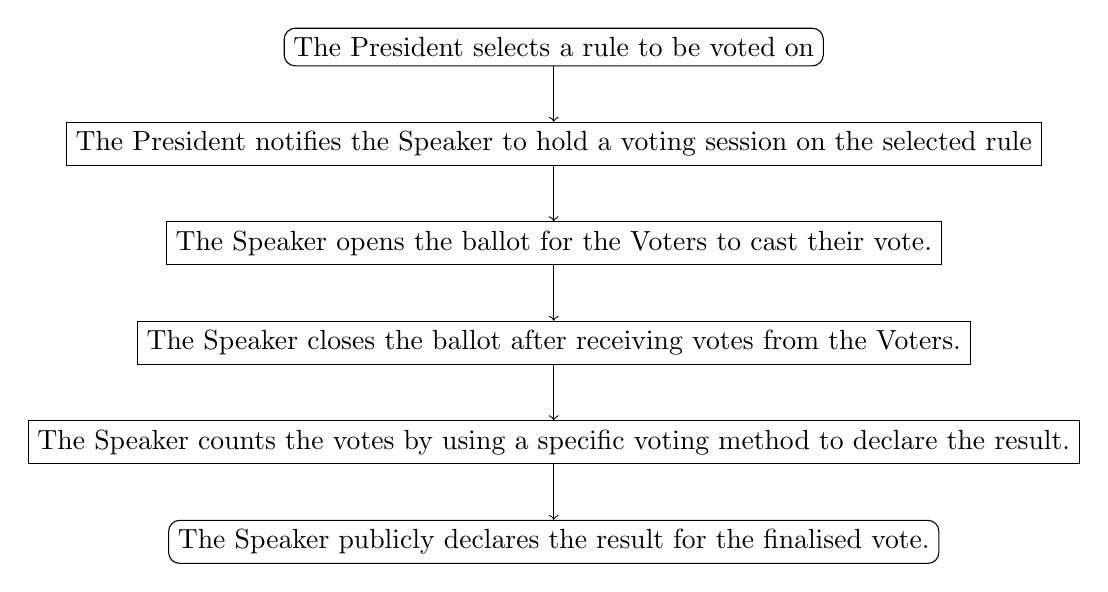
\begin{tikzpicture}[node distance=20pt]
\centering
\node[draw, rounded corners] (start)  {The President selects a rule to be voted on};
\node[draw, below=of start] (step 1)  {The President notifies the Speaker to hold a voting session on the selected rule};
\node[draw, below=of step 1] (step 2)  {The Speaker opens the ballot for the Voters to cast their vote.};
\node[draw, below=of step 2] (step 3)  {The Speaker closes the ballot after receiving votes from the Voters.};
\node[draw, below=of step 3] (step 4)  {The Speaker counts the votes by using a specific voting method to declare the result.};
\node[draw, below=of step 4, rounded corners] (end)   {The Speaker publicly declares the result for the finalised vote.};
 \draw[->] (start)  -- (step 1);
 \draw[->] (step 1) -- (step 2);
 \draw[->] (step 2) -- (step 3);
 \draw[->] (step 3) -- (step 4);
 \draw[->] (step 4) -- (end);
\end{tikzpicture}
\caption{Voting Protocol for Rules}
\label{fig:RONRVotingProtocol}
\end{center}
\end{figure}

For elections of roles, the sequence of actions of the voting protocol is mostly similar to the above explanation in principle, except for some parameters, such as the motion of the vote which is the role itself (President, or Speaker, or Judge), the facilitator of the election/vote event which depends on what role is being held for election (refer to Chapter 5 IIGO for more details on change of roles and power transfer), and the applicable voting method function to call for election that will produce the result, which is different from the voting method used for rules. Refer to Section~\ref{sec:VotingMethods} for more details on voting methods to be used for elections of roles.

At the start of the game, it is assumed that all 6 islands have the power to vote at any necessary voting scenario, and no diplomatic sanction is in place for any island. However, in the further turns of the game, some island(s) could lose their right to vote and/or not permitted to participate in a voting event due to the diplomatic sanction(s) in place. Refer to Chapter 5 IIGO for details on diplomatic sanction. In this case, the Speaker will open the ballots to the eligible islands only , i.e. those who are permitted to vote at a certain state of the game.

% Implmentaion section deleted
\begin{comment}
\section{Implementation}
\label{sec:Implementation}

\subsection{Voting for Rules}
\label{sec:VotingForRules}
The implementation of voting for rules from infrastructure point of view (file:\texttt{rulevote.go}) basically follows the sequence of voting protocol as described in Section~\ref{sec:VotingProtocol}. At initialisation, there are two defined structs (collection of data fields) that are used as parameters for functions inside the voting algorithm, such as \texttt{RuleVote} and \texttt{BallotBox}. The \texttt{RuleVote} struct consists of 3 variables, i.e. \texttt{ruleToVote} (string) that contains the rule that has been selected by the President to be voted on, \texttt{islandsToVote} (list of integers) that contains a list of \texttt{ClientID} which indicates all eligible islands that participate in the voting session, and \texttt{ballots} (list of boolean) that contains the vote of each respective eligible islands where it can indicate the vote for in-favour or against the proposed rule. The \texttt{BallotBox} struct consists of 2 integer variables that act as accumulators for the count of each possible vote: \texttt{VotesInFavour} and \texttt{VotesAgainst}.

According to Section~\ref{sec:VotingProtocol}, The Speaker firstly starts a voting session by calling \texttt{SetRule(rule)} function that contains the rule selected by The President to be voted on. Next, the Speaker sets all eligible islands that can participate/have the right to vote in the voting session at that state of the game by using \texttt{SetVotingIslands(clientIDs[])} function. After that, the Speaker opens the ballots to get the votes from all eligible islands by calling \texttt{GatherBallots(clientMap[ClientID])} function. Subsequently, the \texttt{GetBallotBox()} function is called by the Speaker to gather the ballots that already contain the votes counting of those who are in-favour or against the proposed rule. Finally, the votes counting is concluded by comparing the votes of those in-favour vs those against, and the in-favour votes win when the counting is greater than or equal to the against votes counting, as reflected in \texttt{CountVotesMajority()} function. The Speaker then uses this result to declare the result of this voting session in IIGO.

\subsection{Elections}
\label{subsec:Elections}
The elections for roles implementation can be seen in the file:\texttt{election.go}. At initialisation, there is a defined struct \texttt{Election} that contains 4 parameters, i.e. \texttt{roleToElect} that indicates which role is being voted on (President, or Speaker, or Judge), \texttt{votingMethod} that indicates the voting method being used for the election to determine the winner selection, \texttt{islandsToVote} that contains a list of \texttt{ClientID} which indicates all eligible islands that participate in the voting session, and \texttt{votes} that is a list that contains the order rank of preference of the candidates for the role from each eligible island who casts the vote.

The election session begins by calling the \texttt{ProposeElection(role,method)} function that depends on which role being voted on and which role has obligation to facilitate the election (refer to Chapter 5 IIGO on Change of Roles and Power Transfer sections), and the selected voting method to be used for this election (refer to Section~\ref{sec:VotingMethods} for details on voting methods and Subsection~\ref{subsec:VotingPseudo} for pseudo-code implementation). The election facilitator then opens ballots to all eligible islands to cast their votes by calling \texttt{OpenBallot(clientIDs[])} function. The \texttt{Vote(clientMap[ClientID])} function gathers all the ballots containing the votes from all eligible islands that are obtained from \texttt{GetVoteForElection(roleToElect)} function returned from each client/island code execution. After that, the election facilitator closes the ballots by using \texttt{CloseBallot()} function and it returns the result of the votes counting using the selected voting method by calling each respective voting method function. This result is used by the election facilitator to declare the winner for the elected role. By default, the voting method for election is Borda Count and the function is called \texttt{bordaCountResult()} where the algorithm follows through what are explained in Section~\ref{sec:VotingMethods} and Subsection~\ref{subsec:VotingPseudo} where the Borda scores will be calculated based on the order rank of preference of the candidates from each ballot. The other voting methods can be used for election and it is selected by the election facilitator.

\subsection{Voting Methods Implementation Pseudo-code}
\label{subsec:VotingPseudo}

\textbf{Plurality}
\newline
Call for Voting inputs (int:IslandID, str:"Aye", "Nay" or "Abstain")\\
\begin{algorithm}[H]
\ForEach{$ballot \in ballots $}{
    \If{$Aye$} {Count for $Aye ++ $}
    \If{$Nay$} {Count for $Nay ++ $}
}
\If{$Aye > Nay$}{\Return the Winner: $Aye$}
\Else{\Return the Winner: $Nay$}
\end{algorithm}

\ \newline \ \newline \ \newline
\textbf{Borda Count}
\newline
\begin{algorithm}[H]
\For{all ballot}{
    $numNotIn\gets N-ballot.length$\\
    $shareScore\gets 1+...+numNotIn$\\
    \For{i from 0 to N-1}{
    \If{i is in ballots} {$scores[i]\gets scores[i]+N-K+1$ }
    \Else {$scores[i]\gets scores[i]+shareScore/numsNotIn$ }
    }
}
Sort candidates by Borda scores\\
\Return the candidate with the highest score
\end{algorithm}

\ \newline \ \newline \ \newline
\textbf{Runoff}
\newline
\begin{algorithm}[H]
\For{All $ballot \in ballots $}{
    Select two candidates with most first-placed votes
}
\If{either already has a majority}{
\Return the majority one}
\Else{Each voter selects one candidate of the top 2\\
}
\Return the candidate with the most votes
\end{algorithm}

\ \newline \ \newline \ \newline
\textbf{Instant Runoff}
\newline
\begin{algorithm}[H]
\ForEach{$ballot \in ballots $}{
\For{i from 0 to N-1}{
\If{i is first choice}{$scores[i]\gets scores[i]+N-K+1$}
}
}
\If{candidate in ballots $>1$}{
Remove the candidate with the fewest first
choice votes from the ballots.\\
GOTO the top for next round of counting
}
\Else{\Return the candidate}
\end{algorithm} 

\ \newline \ \newline \ \newline
\textbf{Approval}\\
\begin{algorithm}[H]
\ForEach{$ballot \in ballots $}{
    \For{i from 0 to N-1}{
    \If{i is in ballot} {$scores[i]\gets scores[i]+1$ }
    }

}
Sort candidates by scores\\
\Return the candidate with highest score
\end{algorithm}
\end{comment}
    \chapter{Team 1 Agent Design}

\section{Core Idea}
Team 1 agent was designed around the idea that the agent wants the whole archipelago to survive. However, the agent does have different configurations to allow for some malicious behaviour in order to facilitate some interesting agent interactions.

\section{Emotional state}

The agent's behaviour is affected by what we have termed her \emph{emotional state}. This is governed by the agent's current resources in relation to the living cost.

\begin{table} [htb]
    \centering
    \begin{tabular}{|l|l|}
        \hline
        \textbf{Emotional State} & \textbf{Condition} \\
        \hline
        Happy & Default state \\
        \hline
        Anxious & Current resources under 5 times the living costs \\
        \hline
        Desperate & Agent in critical state \\
        \hline
    \end{tabular}
\end{table}


\section{Opinions on Islands}
As information and resource sharing between islands is possible, it is possible and desirable for the agent to form an opinion of other islands. This be used to gauge the accuracy of information from other islands as well as, potentially, deny resource sharing to islands deemed ``selfish''.

Initially, opinion on all islands is neutral. Over time, through IITO and IIGO, opinions on islands will change. This will affect behaviour in IITO, as well as IIGO voting. Note that positive values correspond to positive opinions while negative values correspond to negative opinions.

\section{IITO Gifts}
When team 1 agent receives a request for gifts, the agent will decide how much to offer depending on the agent's current emotional state and the opinion of that island.

\begin{table} [htb]
    \centering
    \begin{tabular}{|c|p{0.5\textwidth}|}
        \hline
        \textbf{Emotional State} & \textbf{How is IITO handled?} \\
        \hline
        Happy & Agent will give away resources that satisfies the requested amount. Up to a percent of available resources. \\
        \hline
        Anxious & Agent will give away a ratio of the requested amount and its current resources. \\
        \hline
        Desperate & Agent will refuse any gift requests that it receives. \\
        \hline
    \end{tabular}
\end{table}

During IITO, the agent's opinion of other islands is affected. For every gift received, the agent's opinion of the gift-giver increases. However, the agent's opinion of an island can decrease if that island promised a gift and did not fulfil it.

Moreover, if the agent's opinion of an island is very high, the agent can decide to give gifts disregarding the agent's own anxiety. On the other hand, if an opinion of an island is very low, the agent can decide to refuse to send a gift even though the agent is happy.

For increase survivability, team 1 agent will accept any gift offers that it receives.

\subsection{Future Work}
Team 1 agent currently has a very straightforward IITO strategy. Possible alteration to this strategy could include:
\begin{itemize}
    \item Being less susceptible to bribery. The agent should stop increasing the opinion of an island after receiving $X$ amount of continuous gifts.
    \item Stop handing out gifts to islands that are not in critical state.
    \item Being proactive in bribery. The agent will give non-requested gifts to the current president in hopes that this will reduce tax and increase resource allocation from the common pool.
\end{itemize}

\section{IIFO Disaster Prediction}
Disasters can happen deterministically or stochastically (see Chapter~\ref{sec: Disaster} for more information). For an agent, it is important to predict when a disaster occurs so that as much disaster damage is mitigated using the common pool.

When the game starts, the disaster prediction made by the agent is random. This prediction always has a confidence value of $0$. As more disasters occur, a history of disasters is built up. Using this history, the mean disaster position ($x$, $y$), magnitude and period is calculated. A confidence value is calculated along with the mean disaster metrics and shared along with the prediction.

% Add a footnote on website?  https://www.mathsisfun.com/data/confidence-interval.html
The confidence value is calculated by finding the ratio between margin of error and the mean value. The smaller the margin of error, the more confident the agent is in her prediction. Therefore, a difference between the mean value and the margin of error must also be calculated. The confidence interval equation is used to calculate the margin of error:

\begin{equation}
    \label{eq: Team1MarginOfError}
    \textsc{Error} = Z \dfrac{s}{\sqrt{n}}
\end{equation}

where $s$, $n$ and $Z$ are the standard deviation, size of array and confidence interval respectively.

Using the difference between the mean value ($\bar{x}$) and the margin of error and taking the ratio of this result over the mean will provide the agent with the confidence value.
\begin{equation}
    \textsc{Confidence Value} = \frac{\bar{x} - \textsc{Error}}{\bar{x}}
\end{equation}.

The agent maintains a \textbf{trust score} for every island \emph{including itself}. This is based on the accuracy of islands' prediction of time left to the disaster.

Sharing and obtaining other disaster information to and from other islands respectively can increase the survivability of the archipelago. As more disaster predictions are shared, a network of trust between team 1 agent and other islands is built.

\subsection{Future Work}
While team 1 agent has a satisfactory disaster prediction algorithm, it does not make use of this prediction or predictions from other islands in any meaningful way. This is primarily due to disaster prediction being one of the last features to be implemented and not enough time being available to complete it.

Nevertheless, here are some possible uses for the disaster prediction system.

\begin{itemize}
  \item \textbf{Tax policy} --- As president, the agent could choose to increase or decrease taxation depending on (predicted) time left to disaster.
  \item \textbf{Voting} --- A trustworthy island could make for a better president, speaker or judge, as they would be able to act according to imminent disasters.
  \item \textbf{Common pool contribution} --- Based on predicted disaster location the agent may increase or decrease her common pool contribution. If a disaster is expected to affect the agent significantly then she could choose to mitigate resource loss by contributing a large amount to the common pool, as the alternative would be losing more resources.
\end{itemize}

Finally, prediction accuracy could be improved by using the prediction of the most trustworthy island, whether that is the agent herself or not, or averaging the predictions of the most trustworthy islands.

\section{IIGO: President}

Following the agent's core idea, as the president, the agent will try to enlarge the common pool as well as redistribute wealth among the islands, in an attempt to ensure the survival of as many islands as possible. This is achieved through an aggressive, tiered tax policy as well as denying common pool allocation requests to the wealthier islands.

This policy had to be verified as it could be vulnerable to ``free-rider'' islands, who could avoid paying tax and still reap the benefits of disaster protection from a large common pool and ``bailout'' allocations when they are low on resources.

As a test of this, a simulation was set up with a variable number of lawful and free-rider islands in order to measure the stability of this policy.

Three tax evading islands (half of the islands) was found to be the limit at which this policy would lead to collapse of the IIGO and the common pool. This was deemed an acceptable limit as at least half of the other agent teams would obey tax policy, at least most of the time or with a small amount of evasion. The resource graphs for the cases of two and three tax evading islands can be seen in \autoref{fig:team1:two_invaders} and \autoref{fig:team1:three_invaders}.

\begin{figure}[H]
\centering
\includegraphics[width=0.9\textwidth]{09_team1_agentdesign/images/two_invaders}
\caption{Resource graph. Islands 5 and 6 are evading tax.}
\label{fig:team1:two_invaders}
\end{figure}

\begin{figure}[H]
\centering
\includegraphics[width=0.9\textwidth]{09_team1_agentdesign/images/three_invaders}
\caption{Resource graph. Islands 4 to 6 are evading tax.}
\label{fig:team1:three_invaders}
\end{figure}

Note here that collapse of IIGO (as in \autoref{fig:team1:three_invaders}, with three tax evaders) does not automatically imply collapse of the archipelago; the islands appeared to survive (and, in fact, thrive) even after the collapse of IIGO.\@ It was taken as an assumption that this was only due to the uniformity of strategies, and in the ``real'' simulation, with heterogeneous agents, collapse of IIGO would lead to collapse of the archipelago.



\section{Foraging}
Multiple foraging strategies were developed, initially by intuition and later by attempting to address the shortcomings of previous attempts. They were developed in order and aptly named:
\begin{itemize}
    \item Return on Investment (ROI)
    \item Regression
    \item Flip Forage
\end{itemize}


\subsection{Return on Investment (ROI) Foraging}%
\label{sec:forage-roi}

This first algorithm is based on repeating successful foraging behaviours in the past, whether those be by the agent herself or another agent.

For the first few turns (the exact amount is configurable) the agent will forage randomly.

The agent maintains a history of foraging decisions and outcomes, including those received from IIFO.\@ When it comes time to forage, this history is sorted by ROI, i.e.\ the ratio of profit to contribution. Decisions that resulted in a loss, had profit smaller than the living cost, or had a larger contribution than a (configurable) percentage of available resources, are filtered out.

\subsection{Regression Foraging}%
\label{sec:forage-regression}

This strategy tries to predict the ideal foraging decision, even if that exact decision was not made in the past. This is done using regression, which is used to find the decision with the highest expected reward.

The \emph{regression} strategy forages randomly in the initial turns and history is kept as in \nameref{sec:forage-roi}. To make a foraging decision, the history is split by foraged resource (fish or deer), and quadratic regression is performed on contribution versus reward for both resources. From this, a quadratic equation is formed. If the quadratic equation found is negative then the optimal contribution can be found by differentiation. If it is positive then a (large) value is chosen as contribution, as a higher contribution should simply lead to a higher reward.

\subsection{Flip Foraging}

This strategy chooses the least foraged resource from the last turn, according to IIFO-reported data. Contributed amount is proportional to the chosen resource's total ROI from last turn. This choice was made under the assumption that ROI is an indicator of the resource's ``condition''. If a resource only gives moderate rewards (proportionally to input) it means that it is probably over-used currently and as such agents should allow it to recover, by scaling down their foraging attempts or by switching foraging types.

\subsection{Comparison}

To compare the three strategies, simulations were run with six agents, two using \emph{ROI foraging}, two using \emph{regression foraging}, and two using \emph{flip foraging}. IIGO and IITO were also disabled in order to isolate the efficacy of foraging methods from other parts of the game. The simulation was run five times and the results averaged over the 5 games as well as the two agents following the same strategy.

\begin{figure}[H] 
\centering
\includegraphics[width=0.6\textwidth]{09_team1_agentdesign/images/mean_survival_turns}
\caption{Mean survival turns for different strategies.}
\label{fig:team1:mean_survival}
\end{figure} 

\begin{figure}[H] 
\centering
\includegraphics[width=0.6\textwidth]{09_team1_agentdesign/images/total_efficiency}
\caption{Average foraging efficiency}
\label{fig:team1:average_efficiency}
\end{figure} 

It is clear from \autoref{fig:team1:mean_survival} that the \emph{flip} foraging strategy dominates the other two in terms of overall effectiveness. However, it is interesting to note that, according to \autoref{fig:team1:average_efficiency}, the \emph{ROI} foraging method is almost as efficient as \emph{flip}, which raises the question of what causes the difference in their success. This difference could be attributed to one core issue with the \emph{ROI strategy}: ignoring the absolute value of rewards. The agent will happily settle for a profit of $11$ resources, if that was obtained with a contribution of $0.1$ resources (a profit of $110000\%$) over a profit $50$ resources for a contribution of $25$ (a measly $100\%$). This means that in the long run living costs overwhelm the \emph{ROI} agent. The \emph{flip} agent does not take expected profit into account and as such is unaffected by this.

\emph{Regression} appears to occupy a medium between \emph{flip} and \emph{ROI}, however it is much less consistent, as evidenced by the error bars in \autoref{fig:team1:mean_survival}, with \emph{regression} surviving for under 10 turns in some runs.

%%% Local Variables:
%%% mode: latex
%%% TeX-master: "../main"
%%% End:

    \chapter{Team 2 Agent Design}
\section{Overall Agent Strategy}

The overall strategy of our agent is based on a series of distinct, overlapping dilemmas. The agent operates on principles based on Evolutionary Economic Theory \footnote{https://www.cambridge.org/core/what-we-publish/elements/evolutionary-economics}. Game theory and the use of the Nash equilibrium also guided the development of the strategies implemented. The other top-level strategy which overlaps with several dilemmas is the social dilemma; this is when we quantify the relationship we have with other agents to produce trust and confidence levels. The interaction between the top-level strategies with all of the dilemmas is shown in Figure~\ref{fig: top level strategy}. The top-level strategy's implementation into each agent function and role is discussed in the following sections. 

\begin{figure}[!htb]
    \centering
    \subfigure[Top level strategy]{
        \centering
        \includegraphics[width=0.49\textwidth]{10_team2_agentdesign/images/strategies.png}
        \label{fig: top level strategy}    
    }
    \subfigure[Ceremonial-Instrumental dichotomy]{
        \centering
        \includegraphics[width=0.49\textwidth]{10_team2_agentdesign/images/dichotomy.png}
        \label{fig: dichotomy}
    }
\end{figure}

\subsection{Evolutionary Economic Theory}
The term Evolutionary Economic Theory was first coined by economist Thorstein Veblen \footnote{https://www.cambridge.org/core/what-we-publish/elements/evolutionary-economics}. Evolutionary Economic Theory proposes that economic processes evolve, and it rejects the assumptions of classical rational choice theory. From Evolutionary Economic Theory, we categorised agent behaviour into distinct groups \footnote{https://www.cambridge.org/core/what-we-publish/elements/evolutionary-economics}. These groups are an altruist, fair sharer, and free rider. These are explained in Table~\ref{tab:Evolutionary Economic Theory Agent classifications}.


\begin{table}[!htb]
    \caption{Evolutionary Economic Theory Agent classifications}
    \label{tab:Evolutionary Economic Theory Agent classifications}
    \begin{tabular}{|c|m{0.3\textwidth}|p{0.4\textwidth}|}
    \hline
    \textbf{Agent classification} & \textbf{Definition}  & \textbf{Examples within the game} \\ \hline
    Altruist  & More concerned about the welfare of the group than themselves  & \begin{tabular}[p{0.4\textwidth}]{@{}p{0.4\textwidth}@{}}-Contributes a surplus to the common pool\\ -Generous with gifts\end{tabular}                                                     \\ \hline
    Fair Sharer                   & Contributes enough to the group  to negate their negative impact on it & \begin{tabular}[p{0.4\textwidth}]{@{}p{0.4\textwidth}@{}}-Contributes the minimum necessary amount of resources \\ -Gift allocation is measured and reasonable\end{tabular}                          \\ \hline
    Free rider                    & More concerned with their individual welfare than the welfare of the group & \begin{tabular}[p{0.4\textwidth}]{@{}p{0.4\textwidth}@{}}-Will not contribute enough to the common pool \\ -Gift requests above their requirement \\ -Will not give out gifts\end{tabular} \\ \hline
\end{tabular}
\end{table}
    

The advantage of using this theory over rational choice theory from classical economics is that it accounts for the irrational decisions agents or humans make when dealing with economic decisions, such as deciding how much to contribute to a common pool. Humans have evolved to develop heuristics \footnote{\url{https://www.sciencedirect.com/topics/social-sciences/heuristics}} which are "rules of thumb" in order to make economic decisions quickly and when all information is not present. These heuristics are typically based on emotion and will often result in irrational decisions; an example of this would be brand loyalty. This is very relevant within the context of the game because there is a cost to large computations (decision making). Also, there is an information failure \footnote{\url{https://www.economicsonline.co.uk/Market_failures/Information_failure.html}} as the agents often do not know the threshold of the common pool and other vital game metrics. This information failure forces agents to use heuristics similar to those used by real people. An excellent example of a heuristic within this agent strategy is the level of trustworthiness decided within the social dilemma. If every agent was rational and all information was present in the game, there is no need to trust or distrust agents as they would maximize both their welfare and that of others.

Another primary reason for selecting this theory as the basis of our design is to explore the ceremonial-instrumental dichotomy\footnote{\url{https://www.jstor.org/stable/3486187?seq=3\#metadata_info_tab_contents}}. This dichotomy is best represented by the graph in figure \ref{fig: dichotomy} and shows the importance of the game's setup. Our agent is attempting to oppose this traditional response to instrumental and ceremonial societies. It would be interesting to change the game's ceremonial and instrumental values by changing the setup. While the current game infrastructure does not support this, it would be interesting to investigate the ceremonial-instrumental dichotomy by allowing islands to invest resources into developing their foraging technology to obtain higher returns. It would be interesting to investigate how this instrumental shift would change our agent's strategy and others' actions. This update in technology would replace the ceremonial institutional set up of the IIGO as it becomes redundant. Allowing islands to invest in technological advancement would add an extra dimension to the game as it evolves, and the importance of the IIGO and other instrumental components would shift.

\subsection{Evolutionary Economic Theory Implementation}
%explain how we use the information from the theory

Figure~\ref{fig:methods-of-play} shows the different states of our agent's different methods of play. At any point during the game, the state of our agent is determined only by the level of the Common Pool. Our agent's objective is to oppose the strategies employed by other agents to attain stability in the game. To determine the method of play of the other agents, we look at whether the Common Pool is, on average, increasing or decreasing. If the pool is being depleted, it can be assumed that the other agents act as free-riders on average. To counteract this, we act as an altruist (see section \ref{sec:Common Pool Dilemma Strategy} for more detail). The average pool level is used because individual agent strategies are irrelevant for the game's overall course. Within the game, we also do not always have access to individual agents' contributions, which would be needed to classify them individually. This makes the average level of the Common Pool the only viable parameter. 

Our simulations demonstrated that starting the game in a "free-rider" state resulted in optimal agent performance and did not negatively impact the course of the game overall.

The default state for the agent is to be a "fair sharer." The agent will move into altruist mode when the weighted average of the Common Pool has dropped drastically. The agent considers a weighted average to ensure that the agent does not panic after every disaster and over contribute. The most recent turns will also be weighed higher to determine the course of the game. When the Common Pool stops decreasing, the agent will move back to fair sharer mode. Similarly, if the pool's weighted average increases by a large factor, then our agent moves into a free-rider state.

\begin{figure}
    \centering
    \subfigure[Method of Play diagram]{
    \centering
        \includegraphics[width=0.4\textwidth]{10_team2_agentdesign/images/MethodofPlay.png}
        \label{fig:methods-of-play}
    }
    \subfigure[Social Classification Order]{
    \centering
    \includegraphics[width=0.4\textwidth]{10_team2_agentdesign/images/Social.png}
    \label{fig:social-order}
    }
\end{figure}



\subsection{Social Classification}
The agent forms an opinion on others depending on different situations. Initial testing suggested that another island's gift-giving behaviour does not necessarily correlate with their quality of predictions. Consequently, the trust of other agents is computed and stored separately for each situation. The agent uses the weighted average of past interactions with other agents to determine whether to trust them in each situation for future interactions. Using a weighted average to compute trust resulted in notably better agent performance. This is because the agent's trust in other agents considers all interactions with other agents while weighting recent interactions more heavily.

An integer value represents the agent's trust metric for each agent in each situation between 0 and 100, where 100 denotes full confidence and 0 a complete lack thereof. This value is used to compute the expected outcomes of situations. These are then compared with real events to update the agent's confidence in the other agents regarding this situation. For example, when the agent receives predictions from other islands, it computes the weighted average to check whether it trusts the island. Once a disaster occurs, the magnitude or timing of the disaster is compared with the other island's prediction. This reality is used to assess their behaviour and update the trust metric for that island relating to that situation. The list of different "situations" includes how an agent behaves in a role such as the President, Judge, Speaker, gift-giving, and disaster prediction. The overall structure of how the agent forms opinions on other islands is shown in Figure~\ref{fig:social-order}.

\section{Gift Giving and Receiving}
The agent must decide whether or not to respond to other agents' gift requests and how much to request from others through gifting. The implementation does not consider whether or not an agent is critical when requesting gifts and instead considers its current method of play and the trustworthiness of the requesting agent. Figure~\ref{fig: gifts} shows a decision tree for how the agent will allocate or request gifts, in which the agent splits up the gift request among the other agents to increase the likelihood of an agent allocating the gift.


\begin{figure}[!htb]
    \subfigure[Gift Giving and Receiving decision tree]{
        \centering
        \includegraphics[width=0.49\textwidth]{10_team2_agentdesign/images/gifts.png}
        \label{fig: gifts}
    }
    \subfigure[Common Pool Strategy]{
        \centering
        \includegraphics[width=0.49\textwidth]{10_team2_agentdesign/images/common_pool_strategy.png}
        \label{fig: common_pool_strategy}
    }
\end{figure}



Depending on the method of play, the agent will request more or fewer gifts. This is inversely proportional to the number of resources taken from the Common Pool. The agent obtains a larger proportion of its needed resources from gifting than the Common Pool in the altruist state. This is done to mitigate common pool depletion in the interest of the common good. In a Fair-Sharer state, the agent aims to obtain its resource target equally from gifts and the Common Pool. A minor surplus is also included in the resource target to ensure that the goal is met, given that gifts from other agents cannot be guaranteed. In a Free-Rider state, the agent takes the majority of its resources directly from the Common Pool but still requests gifts to build up its resources by taking advantage of relationships with other agents as well as a Common Pool surplus.

The \textbf{Gifts} social classification situation refers to both when an island requests a gift from our agent and when our agent requests a gift from that island. The balance between agent gift requests and responses is used as a basis for opinion formation on another agent. Other agents that fulfill the agent's requests are rewarded with higher trust. The agent's own gift requests tend to be small but are also proportional to its trust in each other agent. Every gift interaction is used to update the agent's trust in another island's gifting behaviour.

\section{Common Pool Dilemma Strategy} \label{sec:Common Pool Dilemma Strategy}
The Common Pool dilemma strategy can be split into two considerations. One consideration is the current method of play (altruist, fair sharer, and free-rider), and the other is the current game state. A decision tree showing the common pool strategy is shown in Figure~\ref{fig: common_pool_strategy}. These considerations decide whether and how much we contribute or take from the Common Pool.

\subsection{Method of play consideration} \label{ssec:Method of play consideration}
The primary consideration for giving to the Common Pool dilemma is the agent's current method of play. The agent's state is determined by the Common Pool level, as seen in Figure~\ref{fig:methods-of-play}. The agent's default state as a "fair sharer" contributes the average amount of other agents to the Common Pool. This is calculated by evaluating changes in the Common Pool level from the previous turn and averaging this quantity by dividing by the number of alive agents. If the Common Pool level decreases, the most recent Common pool increase is used to determine the amount given.

By using the average Common Pool contribution, the agent benefits from the forecasting of other agents. This benefit would arise should another agent have an advanced forecasting prediction that determines the Common Pool threshold and what is required to mitigate the effects of a disaster. In this case, the agent would then contribute a similar quantity of resources. This "herd-mentality" approach relies on the assumption that other agents make rational decisions. So if it is evident that other agents are acting irrationally, the agent deviates from this approach to an alternative state (to become either a free-rider or an altruist).

The agent is in an altruist state when the Common Pool is struggling, which often means that other agents act as free-riders. This is where the meta-strategy of Evolutionary Economic Theory comes into play. It is in the agent's interest to contribute much more to the Common Pool to alter the game's course in a positive direction and prevent the pool from being below the threshold when a disaster occurs. Therefore, the agent contributes more resources to enact this balance on the system. 
The altruist resource contribution is a larger factor of the weighted average contribution and can be tuned using the \emph{altruist factor} variable in the agent's configuration.

In a free-rider state, the Common Pool has a surplus, and the agent assumes other agents are on average operating as altruists. In this situation, the agent contributes less to the Common Pool and preserves resources to mitigate short and long-term risk. Contributing too much to the Common Pool no longer benefits the greater good, as these resources can still be used to forage and generate more resources. Therefore, the agent accumulates resources when others are too generous, allowing greater foraging investments and making it easier to help other agents if they struggle in the future.

The method of play also impacts how the agent decides to take from the Common Pool. After game state considerations are made, the agent adjusts how much it takes from the Common Pool according to its Agent State. Table~\ref{tab:Method of play common pool taking} outlines a summary of how the agent adjusts how much it takes and gives a justification for each action. The amount to take from the pool depends on how willing other agents are to contribute to the agent within the game's gift-giving section.  This means the agent must decide what proportion of the resource request must be taken from the Common Pool and from gifting, and this decision also factors in both common pool allocation as well as gift response predictions. When the agent is in a free-rider state, the common pool has a surplus, and so it makes more sense to take directly from the pool rather than requesting gifts. 

\begin{table}[!htb]
\centering
\caption{Method of play common pool taking}
\label{tab:Method of play common pool taking}
\begin{tabular}{|c|c|}
\hline
\textbf{Agent classification} & \textbf{How this impacts taking from the common pool}                              \\ \hline
Altruist                      & Pool is being depleted, best to not take from the pool                             \\ \hline
Fair Sharer                   & Gift requests and taking from the pool are equal                                   \\ \hline
Free rider                    & \multicolumn{1}{l|}{Pool has surplus, take from the pool rather than gift request} \\ \hline
\end{tabular}
\end{table}

\subsection{Game state consideration} \label{ssec:Game state consideration}
The primary consideration in taking from the Common Pool is the current game state. The key parameters (shown in Figure~\ref{fig: common_pool_strategy}) considered are whether the agent is critical and whether the agent has excess resources. This excess is calculated as the difference between the agent's current resources and the minimum resource threshold and the cost of living. Beyond this minimum resource level, the agent can survive one another turn. If the agent has fewer resources than these aggregated costs, the excess is zero. If there are excess resources, the agent will give some resources to the Common Pool. In this case, a strategic contribution is calculated. If the Common Pool threshold is known, the agent considers how many resources are required to attain this threshold. This is then spread over the expected number of turns until the next disaster is predicted to occur and the number of alive clients. If this is unknown, a default value is used to form an initial guess in the agent configuration. On top of this quantity, a strategic contribution is also calculated (see \ref{ssec:Method of play consideration}). The current method of play determines whether the disaster-determined contribution or the strategy-determined contribution is contributed to the pool. This amount is then contributed together with the current tax, unless there are no excess resources as this implies the agent is in a critical state and so all resources are preserved.

\section{Foraging Dilemma}
The foraging dilemma is split into two parts. One determines whether the agent should hunt or fish, and the other determines how many resources to spend on foraging. The foraging dilemma only depends on the current method of play. The method of play will impact the amount the agent uses to forages. If the Common Pool is doing well and the agent acts as a free rider, it will be more prone to take risk and contribute more to the foraging and vice versa. The decision to hunt or fish depends on the likely number of hunters in the next foraging event. The decision tree, Figure~\ref{fig: Hunt or fish decision tree }, shows how the agent decides whether to hunt or fish in a given turn. To determine the number of hunters in the next forage turn, the agent tracks how often each agent is a hunter and then sums up the probability of each agent hunting to find an overall number of likely hunters. The agent outputs a random number from 0 to 1, and if the number lies above the threshold, the agent will hunt. This threshold is determined by the number of likely hunters in the foraging. It implies there is an element of randomness to the agent's decision making, which will account for the unpredictability of dealing with other agents with their strategies.

\begin{figure}[!htb]
    \centering
    \subfigure[Hunt or fish decision tree]{
        \centering
        \includegraphics[width=0.4\textwidth]{10_team2_agentdesign/images/forage_decision.png}
        \label{fig: Hunt or fish decision tree }
    }
    \subfigure[Roles Decision Tree]{
        \centering
        \includegraphics[width=0.4\textwidth]{10_team2_agentdesign/images/Roles Decision Tree.png}
        \label{fig: Roles Decision Tree}
    }
    \caption{Hunting or Fishing and Roles Decision Tree}
\end{figure}



The ideal distribution for foraging is to have two agents hunting and the remainder fishing. Hence, when the agent predicts one other agent will hunt, the agent is highly likely to choose to hunt too. The default threshold for hunting is 0.1, so the agent will hunt 10\% of the time when not considering the likely number of hunters. By assuming that any agent will hunt or fish with equal probability, the likelihood that there is one hunter is approximately 0.16. This implies hunting is an optimal strategy approximately 16\% of the time, so a threshold similar to this value is chosen. If the predicted number of hunters is above one, the following equation is used to determine threshold placement: $\text{Probability of agent hunting} = 0.95 - \text{Predicted number of hunters} \times 0.15$

The probability of choosing to hunt when the agent is confident only one other agent will also select hunt is 0.95. For each additionally predicted hunter, the probability will fall by 0.15. This 0.95 threshold is included in the agent configuration so it can be edited without changing the code. Hence, the foraging decision can be tuned. The agent checks if there are any excess resources after considering the minimum resource threshold not to be critical and the cost of living. If there are no excess resources, no resources are spent on foraging. If there is an excess of resources, a percentage of this excess is used on foraging. This percentage is controlled in the agent configuration. This approach ensures the agent has enough resources to survive another round, even in the worst case scenario when foraging returns are minimal.

\section{Role Strategies}

Figure~\ref{fig: Roles Decision Tree} shows a decision tree of how the agent acts under the two roles implemented. Due to time constraints, the base client implementation was used for the Speaker. The President is responsible for allocating resources from the Common Pool based on agent requests. The agent uses game state variables such as their critical status to determine if another agent is worthy of their resource request and the agent's allocation method based on the method of play is outlined in Table~\ref{tab:President allocation method of play}. When the agent is in a free-rider state, it is more selfish, while when it is an altruist, more of the others agents requests are approved. If an agent is not critical, it is highly unlikely that the agent will allocate them their requested resources as the purpose of the Common Pool should be to primarily mitigate the effects of disasters. Resources are allocated on a need-first basis, taxed proportionally to an agents resource level, and the strategy to determine taxation includes an additional penalty tax for agents who do not declare their resource levels. When evaluating another President's performance, the agent considers the percentage change in tax, the percentage of how much the agent is allocated with respect to how much it requests, and how much the agent takes with respect to how much the President allocates it.

\begin{table}[!htb]
\centering
\caption{President allocation method of play}
\label{tab:President allocation method of play}
\begin{tabular}{|c|c|}
\hline
\textbf{Agent classification} & \textbf{\% of request given} \\ \hline
Altruist                      & 60                           \\ \hline
Fair Sharer                   & 50                           \\ \hline
Free rider                    & 40                           \\ \hline
\end{tabular}
\end{table}

The agent implementation of the Judge evaluates whether an agent has broken any rules, as it should. However, to model real world corruption, the agent does not sanction agents that break rules if it considers them to be highly trustworthy (i.e., with a trust score above 80\%). The agents behaviour as a Judge is also determined by its state; when the agent is a free-rider, it sanctions fewer islands. The \textbf{Judge}'s situation, similar to the President, is used by the agent to determine what island to vote for as Judge. This is done by checking the past sanctions the agent received and their duration, to maxmimise personal benefit. The \textbf{RoleOpinion} social classification situation is used when the agent is the Judge and must decide whether or not to pardon other islands' sanctions, whom to choose as the next President whether or not an island has adhered by the rules. The Judge receives information for each island, such as the difference between how much an island contributed to the common pool and how much said they would. The agent uses these differences as a Judge to determine whether or not an island is trustworthy. During a role election, the agent checks its trust in the candidates for the appropriate situation, i.e., the situation when an agent is "President" for a future Presidential election. The agent will return a list of candidates in decreasing order of preference determined by the social classification. To do this, the agent sorts the candidates in terms of how much it trusts them.

\section{Disaster Prediction}
It is important for the agent to be capable of predicting both the severity and timing of disasters, in order to effectively make decisions for contributing to both the common pool and gifting resources to other agents.

Since the simulation is constructed through a series of successive turns, the occurrence of disasters throughout the game can be seen as a Binomial distribution: $D \sim \text{Bin}(n,p)$. In this equation, $D$ describes the number of disasters that occur, $n$ is the number of turns played and $p$ is the probability of a disaster occurring on a given turn.

The aim of our agent is to estimate the number of turns between disasters. We will denote this random variable as $T_D$, with our agent's aim being to find $E[T_D]$. To do this, our agent must estimate $p$. Therefore we have programmed our agent to find the Maximum Likelihood Estimator of $p$ for a Binomial RV\footnote{https://stats.stackexchange.com/questions/191444/variance-in-estimating-p-for-a-binomial-distribution}: $\hat{p} = \frac{D}{n} = \bar{X}$, where $\bar{X}$ is the sample mean of the RV $X$. The expectation of $T_D$ can be estimated using\footnote{https://math.stackexchange.com/questions/1299465/proof-variance-of-geometric-distribution}: $\hat{\mu}_{T_D}= \frac{1}{\hat{p}} = \frac{1}{\bar{X}}$. Thus, this is the optimal estimator for our agent to predict the number of turns between disasters. Furthermore, the confidence that our agent has in this prediction should be inversely proportional to the variance of $T_D$, i.e. how much does $T_D$ vary from the expected value we have found above? The expression for this variance is given below$^2$: $Var(T_D)= \frac{1-p}{p^2}$. 

However, given that our agent does not know the actual value of $p$ used in the simulation, our agent instead estimates the variance using: $\hat{\sigma}_{T_D}^2= \frac{1-\hat{p}}{\hat{p}^2}$. Now that an expression for the estimate of this variance has been obtained, two questions remain: ``what about the variance in $\hat{p}$" and ``how is this variance translated into a confidence value?" The variance of $\hat{p}$ is given by the following expression: $Var(\hat{p})= Var(\bar{X}) = \frac{Var(X)}{n}$. As previously, we do not know the exact value of $p$, making a calculation of $Var(X)$ impossible. However, we can make use of the fact that $Var(\hat{p}) \propto \frac{1}{n}$, by making our agents confidence in the prediction proportional to $n$ also. Secondly, the fact that variance can take values $\in [0,\infty]$ but confidence must take a value $\in [0, 100]$ makes mapping the values of variance that our agent calculates, to a confidence level, challenging. The solution our team opted for was to cap the max value of variance to some value $v_{cap_{T_D}}$, before translating this variance into a corresponding confidence value. This process is given by the equation below: $\text{confidence}_{T_D} = 100 - \frac{100 \cdot \text{min}(\frac{\hat{\sigma}_{T_D}^2}{kn}, v_{cap_{T_D}})}{v_{cap_{T_D}}}$ 
where $k$ is the tuning parameter for altering the dependence of the confidence on $n$. 

\subsection{Magnitude Prediction}
Our agent's strategy for predicting the magnitude of the next disaster shares many similarities with the strategy discussed in the last section. However, the magnitude of the next disaster is now distributed with an Exponential distribution: $M \sim Exp(\lambda)$. Once again, start by finding the MLE for the parameter $\lambda$ \footnote{https://en.wikipedia.org/wiki/Exponential\_distribution}: $\hat{\lambda} = \frac{1}{\bar{M}}$. Now we seek to estimate the expectation of $M$: $\hat{\mu}_M = \frac{1}{\hat{\lambda}} = \bar{M}$. Similarly, the variance of this RV is also useful to estimate $\hat{\sigma}_{M}^2= \frac{1}{\hat{\lambda}^2}$. As previously, there is also a variance in our estimation of $\hat{\lambda}$ that must be taken into account by making our confidence in this prediction proportional to $n$. Thus, the following expression should be used for calculating the confidence in the magnitude prediction: $\text{confidence}_M = 100 - \frac{100 \cdot \text{min}(\frac{\hat{\sigma}_{M}^2}{gn}, v_{cap_M})}{v_{cap_M}}$, where $g$ is the tuning parameter for altering the dependence of the confidence on $n$. 

\subsection{Overall Prediction}
The overall prediction that must be shared with teams during the IIFO session requires the following information: location, time until next disaster, magnitude and confidence. For our prediction of location, the middle of the archipelago is always given since the probability of a disaster occurring at a given location is uniform across the archipelago, meaning that there is no optimal prediction formula. Using the findings presented in the above sections, the formulas our agent will use to form a prediction about the next disaster are as follows:

\begin{align*}
    &x_{coord} = x_{min} + \frac{(x_{max}-x_{min})}{2}, y_{coord} = y_{min} + \frac{(y_{max}-y_{min})}{2}, \text{conf} =\frac{\text{conf}_{T_D} + \text{conf}_M}{2} \\
    &\hat{\mu}_{T_D}=\frac{1}{\bar{X}}, \hat{\mu}_M = \bar{M} \\
\end{align*}

\subsection{Combined Prediction}
Generating our own prediction is only the first part of the prediction making process. The second stage is to make use of other island's predictions during the IIFO session and using the social classification to decide prediction accuracy. When considering how much emphasis to put on a given island's prediction, we make use of two factors: 1.) Our island's confidence in each other island's prediction making. 2.) Each island's confidence in their own prediction, $P_i \in [0,100]$. These two considerations are then combined to create an overall confidence factor.

\section{Simulations}
Every function and agent consideration has tuneable parameter which can be edited without changing the whole agent. Figure~\ref{fig: Forage Untuned} shows how our agent reacts when it plays against itself and the foraging parameters are untuned. As you can see the game is unstable and the agents have a low survival rate. This is caused by an over contribution to the foraging dilemma, there is a point of marginal return with the foraging dilemma and spending too many resources can be wasteful. 

\begin{figure}[!htb]
    \centering
    \includegraphics[width=0.6\textwidth]{10_team2_agentdesign/images/Forage Untuned.png}
    \caption{Untuned Forage Simulation}
    \label{fig: Forage Untuned}
\end{figure}

Figure~\ref{fig: Forage tuned} shows how our agents plays against itself when the foraging parameters are optimised. The amount of excess resources spent on foraging is more reasonable in this simulation, this results in a much higher survival rate and a more stable common pool.

\begin{figure}[!htb]
    \centering
    \includegraphics[width=0.6\textwidth]{10_team2_agentdesign/images/Forage tuned.png}
    \caption{Tuned Forage Simulation}
    \label{fig: Forage tuned}
\end{figure}

Figure~\ref{fig: altruist sim}  shows what happens when the agent plays itself and they are all altruists by default and do not move out of altruist. It can be seen that the agents over contribute to the Common Pool and are left with nothing to forage, this ends the game rather quickly. The simulation result was very similar for when all of the agents were free riders, the game would end in a couple of rounds after a lack of contribution to the common pool which caused impactful disasters.  This proves that being a free rider or altruist is not a rational decision and must be avoided. 

\begin{figure}[!htb]
    \centering
    \includegraphics[width=0.7\textwidth]{10_team2_agentdesign/images/altruist sim.png}
    \caption{Altruist simulation}
    \label{fig:  altruist sim}
\end{figure}
    % \newcommand{\subsubsubsection}[1]{\paragraph{#1}\mbox{}\newline}
% \setcounter{secnumdepth}{4}
% \setcounter{tocdepth}{4}


%TODO: Please DO NOT RESOLVE the comments unless you are 100% sure everything related to the comment is resolved, as they can't be retrieved.
%TODO: VERY VERY IMPORTANT: talk to people in our group to make a decision on understanding of the "lack of variety"  that is shown in the comment on line 276 of this latex file. This will cause quite a few changes in the report but it is a very important concept to clarify to avoid burning ourselves. Read all the comments Mike made in the relevant sections first.
%TODO: VERY IMPORTANT: another potential self burn area. Clarify with Rudolfs about Ostrom's Principles after looking at all the comments Mike has made in that section.
%TODO: add in rule distance calculation explanation? It's kinda primitive though
%DONE: President by Andrzej, do talk about disaster prediction
%DONE I THINK: Toby to finish all foraging related stuff (IIFO and End of turn)
%DONE: add in the use of disaster prediction somewhere if we can?
%DONE: to finish IITO and gifting, sneak in disaster prediction if possible - This is done except for the disaster prediction part. Not sure how to add it though, but feel free if you have an idea how.
%TODO: clear up all the TODO's scattered around in this latex file.


\chapter{Team 4 Agent Design}   \label{chap:team4}
Given that our team invested a significant amount of time in ensuring feature richness and stability of the infrastructure, we were left with a short time-frame for our agent's implementation and design. Therefore, at times we had to make decisions that guaranteed canny usability, rather than sophistication. For some actions, our agent relies on other teams' agents with different strengths to perform well. 

\section{Agent overview}
An agent uses the interface that is defined in the infrastructure. In order to define custom behaviours for our agent, we override or extend the base agent (\texttt{baseclient.go}) functions which implement the defined interface. The team built the agent design upon a set of internal fields that aid the decision-making process for the actions it performs. Information to describe the agent's personality is recorded in a structure of internal parameters, namely \texttt{Greediness}, \texttt{Selfishness}, \texttt{Fairness}, \texttt{Collaboration} and \texttt{RiskTaking}, all of which have decimal values between 0 and 1. The agent stores observations, histories as well as other necessary information such as its trust in others. These internal fields will be discussed in more detail in the following dedicated sections. %TODO: add in evolutionary economic theory background for agent personality

An agent can be elected in one or more positions of power inside the IIGO session, and be able to perform the duties of the office. From an infrastructure standpoint, these actions are implemented as overridable functions in the same fashion as previously discussed for the base agent. Although the code was design to differentiate a commoner agent and roles in separate structs, they all share read and write access to the internal fields of each other through pointers. In other words, an agent is always a commoner agent, and a commoner agent can be elected one or more role(s) at the same time.

\section{Opinion formation -- Trust}
\label{sec:team4:trust}
Trust is the score $[0..1]$, which represents the agent's opinion towards fellow agents in the game. This metric helps it in making decisions throughout the game based on how trustworthy, helpful or friendly it believes other agents were. This generic opinion about an island is formed dynamically based on three recurring observations:
\begin{itemize}
    \item The gifts received from the island during the IITO sessions.
    \item The outcome of monitoring positions-of-power when conducted as a part of the accountability cycle.
    \item The evaluation of IIGO actions history, only available to the Judge. This is further explained in Section \ref{subsec:team4:judge}
\end{itemize}
Those observations allow the agent to quantitatively reason about both friendliness of other islands towards it, as well as how closely they follow the rules in play.

The average trust score is forced at a value of $0.5$. Such normalisation ensures that the trust is always balanced throughout the game. It prevents the inflation of trust in a scenario where several islands decide to exchange gifts with the agent. Furthermore, the number of resources gifted will be a deciding factor when updating the trust metrics.

Some decisions made by our agent can be altered based on the trust score towards certain islands. During elections, if the trust of an island is lower than a specified threshold, the agent will never cast its vote in favour of it. Similarly, if holding the role of Judge, it will choose not to act upon its power to pardon the island with a low trust score.

On the other hand, if the agent holds a good opinion about an island, it may choose to favour it by providing or even deciding to  pardon it from a sanction.


\section{IIGO}
\subsection{Commoner Agent} \label{commoneragent}
At the start of any IIGO, each (commoner) agent is prompted by the president to report how many resources it has. Our agent overrides its reporting behavior  to account for several internal factors, as further discussed in subsection \ref{reportresources}. The president uses this information to set a taxation amount according to each agent's self-report, notifying them of the tax demanded. Each (commoner) agent can later send a request for the specific amount of resources it aims to retrieve from the Common Pool (an allocation request) to the President. Upon receiving a response from the President on the actual amount that was granted, the agent is allowed to access the Common Pool. The actions concerning requesting and taking allocations are overridden, as part of the agent strategy. Due to a design decision, the action for taking allocations and paying tax does not happen within the IIGO session, it happens after all organisations are run, inside the \texttt{EndOfTurn} session.

\subsubsection{Report Resources} \label{reportresources}
When reporting its resources, our agent uses a weighted linear combination of some of its internal fields. The weighting of each parameter is defined as an array of real values called "importance" and stored in an \texttt{importance} vector. The linear combination outputs a scaling factor to divide to the actual resources our agent has, as shown in \eqref{linear_comb}, in order to compute an untruthful amount to report to the President. The parameters used are \texttt{greediness}, \texttt{selfishness}, \texttt{fairness}, \texttt{collaboration}, \texttt{riskTaking} and trust in the current president (all values are between 0 and 1). Some fields are associated with negative weights as they should logically negatively impact the scaling factor. The greater the absolute value of weight, the bigger impact it has on the scaling factor.

\begin{equation}\label{linear_comb}
    \begin{bmatrix}
        w_{1}& w_{2}& w_{3}& w_{4}& w_{5}& w_{6}
    \end{bmatrix}
    \cdot
    \begin{bmatrix}
    Greediness \\ 
    Selfishness \\ 
    Fairness \\ 
    Collaboration \\ 
    RiskTaking \\
    TrustScore_{President}
    \end{bmatrix}
    = Scaling\:Factor
\end{equation}

To decide when to lie, the scaling factor is first compared to a preset threshold. If the scaling factor is greater, then the amount of the needed resource is divided by 
\begin{equation}
    [1 + (Scaling\:Factor - Preset\:Threshold)]
\end{equation} 
This conditional statement makes sure that the scaling factor is not always applied, ensuring that our agent will lie on its resources only when deemed a good strategy.

\subsubsection{Paying Tax Contribution}
%write about this and the lying mechanics
The \texttt{GetTaxContribution()} function returns the amount an agent is paying in tax. Similarly to resource reporting, the tax amount is modified by a scaling factor applied only when greater than a preset threshold, as shown in the following equation: 
\begin{equation}
    [1 + (Scaling \: Factor - Preset \: Threshold)]
\end{equation}
Based on the preset weighting for internal parameters, this situation is likely to arise when the \texttt{Collaboration} of our agent is high. In addition, the scaling factor is not applied when the tax demanded is more than $\frac{1}{5}$ of the agent's resources. This prevents it from generously giving out most that it has.

\subsubsection{Requesting Allocation}\label{subsubsection:CommonPoolResourceRequest()}

The aforementioned action of requesting resources from the common pool is implemented in the function: \texttt{CommonPoolResourceRequest()}. When requesting an allocation, our agent first decides what it needs. When not in a critical state, the needed resources are usually a multiple of the basic needs, namely the cost of living plus the critical threshold. This amount is decided so that the agent always takes more from the Common Pool than their definite expenses in the next turn. If critical, the agent will ask for a bigger multiple of the basic needs. This design choice maps the following logical conclusion that the agent draws from the history of the game: if the a smaller multiple when made the agent critical, it must take more to invert the negative trend in resources. In order to avoid draining the Common Pool, our design enforces that what our island needs must not exceed the number of resources in the Common Pool divided by the number of agents alive. This is to avoid our agent selfishly monopolising the Common Pool resources.

\subsection{President}
\label{subsec:team4:president}
Our agent implements a budget-conscious and rule-obeying President. The main changes, compared to the basic implementation include taxation and resource allocation considerations.

\subsubsection{Tax distribution}
When deciding tax amounts for the different island, the President considers the following variables:
\begin{itemize}
    \item amount of resources in the common pool
    \item the financial status of the island
    \item predicted disaster time and magnitude.
\end{itemize}

The President will abstain from setting taxation for islands in a critical state or in a situation when the resources in the common pool can fully mitigate the predicted damage caused by the next disaster. 

Similarly, when the common pool cannot mitigate the next disaster, the President will set taxation for all non-critical island to bring the common pool back to the safe level. In this case, the taxation amount will be higher the sooner the disaster is predicted to occur.

\subsubsection{Common pool resource redistribution}
In order to fairly redistribute the resources placed in the common pool, the President primarily considers the financial status of an island. In other words, the priority in access to the common pool is given to islands in the critical state. 

To ensure the largest possible satisfaction within the archipelago, the islands with smaller requests are given priority. This decision ensures that the highest possible number of agents will be satisfied with their allocation.

The President is also reluctant to allow any resource allocations if the disaster is predicted to occur soon. This, combined with the tax policy, ensures lower damages to the archipelago in the case of disaster.


\subsection{Judge}
\label{subsec:team4:judge}
The Judge implementation provided by our agent can be described as \emph{honest, but curious}. In other words, it follows the rules currently in play, and follows its obligations, however, it extracts the information exclusive to the Judge to reason about other agents in the game. An example of such actions is explained in greater detail below in this Section.

The judiciary functions overloaded from the \texttt{basejudge} implementation are:
\begin{itemize}
    \item \texttt{InspectHistory}, which examines rule violations of all the agents.
    \item \texttt{GetPardonedIslands}, which considers reducing the sanctions for some agents at judges discretion.
    \item \texttt{CallPresidentElection}, which initialises \emph{transfer-of-power} of the executive branch.
\end{itemize}
An explanation of the implementation of those functions is presented below.

\subsubsection{IIGO history inspection}
\label{subsubsec:team4:judge:inspect_history}
In the basic implementation, a history of IIGO actions of all the agents is passed to the Judge for inspection, which could become grounds for introducing economic sanctions for non-rule-obeying players. 

Judge truthfully evaluates and reports the rule violations for each of the agents, just as the \texttt{basejudge}. However, it also extracts and saves the information about the private resource pools of all the agents, taxes they were expected to pay, as well as the actual amount paid to the common pool. Additionally, it stores the \texttt{LawfulnessRatio} of each agent, which is defined as:


\begin{equation}
    lawfulness_{i} = \frac{number\:of\:rules\:obeyed\:by\:the\:agent_{i}}{total\:number\:of\:rules\:inspected\:by\:the\:judge\:for\:agent_{i}}
\end{equation}

where $agent_{i}$ denotes the $i^{th}$ agent in the game.  

The \texttt{LawfulnessRatio} is then used to update our agents' trust towards other islands, thus influencing decisions in different parts of the game. 

\subsubsection{Consideration of pardons}
Compared to the \texttt{basejudge}, which does not grant any pardons and requires islands to pay economic sanctions in full, our implementation of the Judge allows for the pardoning of certain islands. We consider three parameters when deciding whether and the island could be pardoned:

\begin{enumerate}
    \item The severity of the sanction - only sanctions lower than specified severity level can be considered to be pardoned. This ensures that our Judge never pardons an island, who notoriously breaks the rules of the game and gets sanctioned for it.
    \item Time served on the sanction - the Judge will only remove the sanction if at least the specified number of turns has been served by the island. This still allows us to have a punishment for not obeying the rules but also ensures that an island can begin to contribute again earlier.
    \item Trust towards the island sanctioned - only islands, which are considered trustworthy by our agent can be pardoned. The threshold is tuned by an internal parameter of our agent.
\end{enumerate}

An island can be pardoned by our implementation of Judge only if they meet all three requirements presented above. 


\subsubsection{Presidential elections}
The \texttt{basejudge} implementation called an election every three turns, no matter how long the presidential term was. Our Judge implementation improves on that by calling an election only under two conditions:
\begin{enumerate}
    \item The term of the president has ended.
    \item The president did not fulfil its obligations and was dishonest while holding the executive office. It is decided based on the monitoring results coming from the accountability cycle.
\end{enumerate}

This implementation could be further improved to facilitate the \emph{trust} metrics, explained in Section~\ref{sec:team4:trust}. An example of such an improvement would be allowing the president to hold the office longer than its turn if he is most trustworthy according to our internal \emph{trust} metrics.

\subsection{Speaker}
Given the Speaker's role of deciding agendas and announcing the results of the voting, the only viable customisation option in making our custom Speaker seemed to be implementing corruption - in other words, rigging voting results. Other than the obvious reason of avoiding the risk of getting sanctions, we decided against implementing this function into the Speaker's role because in an actual governmental environment, while misprints have occurred and on occasion shaped past history, announcing false results are a very noticeable and easily rectifiable offense. This would be in the disinterest of either honest or dishonest agents. On this note and the following point, it could be said that our Speaker implementation can be described as \emph{honorable and efficient}.

\subsubsection{Action prioritisation}

Our Speaker implementation builds upon the \texttt{baseSpeaker} on a key point: partitioning of budget. The Speaker prioritises the proper running of IIGO in the case of a low budget situation by prioritising its actions according to the rules in play, reflecting the priorities decided by the archipelago. This is done not by changing the actual running order of IIGO (which would require altering the orchestration) but rather enabling/disabling certain actions based on their priorities and cost. Prioritising actions where rules are in play would stop the speaker from performing non-moderated actions instead of actions relating to rules that are still in play. This function is crucial due to the following reasons:
\begin{itemize}
    \item Not performing monitored actions will result in sanctions, harming the agent's resource pool.
    \item The rules are a representation of the archipelago's expectations, thus not following said priorities is a sign of incompetence - damaging the agent's reputation.
\end{itemize}
Since these reasons are applicable regardless of honesty, these mechanics are always implemented regardless of the chosen personality type.

\section{IIFO}\label{sec:team4:IIFO}
%I recommend that we write in the order of function execution order. (the end of turn functions that are related to IIFO should be written inside the EndOfTurn section)Only mention the functions that are worth mentioning. For execution order check the ./doc/EXECUTION_ORDER.md file in the SOMAS repo -- Mike

\subsection{Making Disaster Prediction}
The agent makes predictions about future disasters by getting the mean coordinates, magnitude and number of turns per disaster (i.e. $\frac{1}{freq}$) from the previous disasters. It then computes a \texttt{confidence} score based on these mean values. The \texttt{confidence} score has a range between 0\% and 100\%. The sum of square of difference between the actual value and the mean value for each of the 4 prediction values types(coordinate x, coordinate y, magnitude and turns) is calculated as below:
\begin{equation}
    total = \sum_{i=1}^{len(past\_disasters)}(Value_i - Mean_i)^2
\end{equation}

The above is done for each of the 4 prediction values types. This returns a measurement of the distance between the predicted value (mean value) and the corresponding past disasters' values. The computed sum of square of difference (a measure of distance) is normalised with a max distance (see equations \ref{max_distance:1} to \ref{max_distance:3}) for each of the 4 value types, 100\% minus this percentage value is the \texttt{confidence} score. The \texttt{confidence} score for the prediction is the average of the 4 \texttt{confidence} scores.

Note that the Central Limit Theorem can be applied in this calculations since we assume different disasters are independent. Namely, the higher the distance between a prediction and samples, the less likely it is for this prediction to be true. And with the CLT assumption, the underlying random variables of the value types (uniform RV for coordinates, geometric RV for both magnitude and turns) do not matter. The calculation of the unique preset threshold is below:
\begin{equation}\label{max_distance:1}
    distance_1 = \sum_{i=1}^{len(past\_disasters)}(ValueMax - Mean_i)^2
\end{equation}
\begin{equation}\label{max_distance:2}
    distance_2 = \sum_{i=1}^{len(past\_disasters)}(ValueMin - Mean_i)^2
\end{equation}
\begin{equation}\label{max_distance:3}
    max\: distance = max (distance_1, distance_2)
\end{equation}

By doing the above unique threshold calculation for each value type, we are setting the predicted values out of bounds to have confidence 0\%. (Note: ValueMax and ValueMin are set in game config)

\subsubsection{Making prediction based on other agents' predictions}
Our agent then receives prediction information from all other agent that sent their information to us. A weighted average (based on trust) of these prediction values are calculated to form our final prediction values.

%Theoretically, We would use  a normal distribution to approximate the sampling distribution of the disaster random variable, which is assumed to be independent across turns, justified by the Central Limit Theorem. And by feeding  calculation approximated to be 


% Foraging functions %
\subsection{Sharing foraging information} \label{sec:team4:IIFO:forage}
IIFO also contains the ability to communicate about the foraging information. As we will go further into in Section~\ref{sec:team4:forage},
we choose to overload both MakeForageInfo and ReceiveForageInfo. In the receive function, we store the received values to a map to be used later when making a decision on which foraging method to go for. 

As we use the foraging information from other teams, our island will also communicate our results to the others. However, we only share with islands that shared with us in the previous round, as well as the island that we trust. Our island is completely truthful for this part and will always report which foraging method we went for, as well as how many resources it generated.

\subsection{IITO}
%(put and modify this to fit it somewhere in this section) If our agent is not in a critical state, it requests extra resources in addition to its own wanted resources in an intention to gift to other agents to earn their trust. If this allocation request is approved by the President, it proceeds with the gifting. These gifted resources are given on top of the normal gifts if there are any.
% some rough comments about IITO from Fabio: gifting pool is the key concept. same as president for allocation. Prioritise agents that are critical. Look at our selfishness and current resources. Help critical first(full amount no matter the trust). If not critical, only gift if trust > 0.5
In IITO we handle the process of sending, receiving, and requesting gifts.
Our island has an internal wealth goal which is calculated using our internal greediness and selflessness parameters. If our private pool is smaller than our wealth goal we ask for gifts from the other islands. The amount we ask for is related to the difference between the private pool and wealth goal. If we are in a critical state, however, we ask every island for two times the resources we estimate to be a safe resource level in the hope that at least one island will support us. 

When an island requests a gift from us we first check how many resources we can spare. This is once again calculated by taking the difference between the private pool and the wealth goal. We also look into its trustworthiness. If the island is critical, we prioritise that island. After that, we only return the gift relative to their trustworthiness. 
In addition, when we request allocation in IIGO, we request a bit extra which we gift to other islands in the hope that it will increase our reputation. This is only done if the president permits us to take the extra resources. 


 

\section{End of Turn}
\subsection{Taking Allocation}
This RequestAllocation() function for taking allocation from the Common Pool. After running all of the organisation sessions, the agent then calculates what it wants based on what it needs, and takes what it wants from the Common Pool. A scaling factor is calculated using a linear combination of weights and internal fields. When the scaling factor is above a preset threshold, it is applied similar to in Section~\ref{subsubsection:CommonPoolResourceRequest()}.  %talking about scaling factor calculation briefly, the detailed explanation is already done in ResourceReport. %%We use a linear combination of some of the agent's internal fields, and weights (put inside an \texttt{importance} vector) we set for each of the chosen internal fields to obtain a scaling factor to multiply the needed resources with. The parameters used are \texttt{greediness}, \texttt{selfishness}, \texttt{fairness}, \texttt{collaboration}, \texttt{riskTaking} and trust in the current president (all values are between 0 and 1). The weights have real values. For this particular function, we set the weights to be $5, 5, -5, -5, 1, 5$ respectively. The fields with negative weights negatively impact the scaling factor and vice versa. We deem riskTaking less important than other fields in the calculation of this function's scaling factor. The scaling factor is then compared to a preset threshold. If the scaling factor is greater, then the needed resources amount is multiplied by 1 plus the difference between the scaling factor and the preset threshold. The threshold is there to make sure that the scaling factor is not applied all the time, as we don't want our agent to take more than what it needs all the time.

\subsection{Forage} \label{sec:team4:forage}
As mentioned at the start of the chapter, due to the interest of time, our foraging strategy relies on other islands to make intelligent decisions about the foraging strategy. In short, rather than looking at the game configurations to try to intelligently figure out which method to go for and how many resources to generate, we look at other teams' return ratios to decide for ourselves. As will be discovered in the simulation section (\ref{sec:team4:simulation}), our foraging strategy works very well against the other islands created by the other teams, but not so well when we simulate six of our own islands.  

Our foraging strategy is split into two sections. Managing foraging communications is stored inside \texttt{IIFO.go} and our foraging decisions are stored inside \texttt{Foraging.go}.

As mentioned in Section~\ref{sec:team4:IIFO:forage}, 
the foraging is split into two parts, decision, and return. In the return, we store the results we receive into an array so that we can later use them in the decision making. This is also what we do inside IIFO when we receive the foraging results from the other teams. 

To decide whether to go fishing or to hunt deer the island looks at both its return history as well as looking at the return results received from the other teams. Our island does this is by calculating the return ratio of each island over the past three turns as well as our own. These ratios are then compounded into two separate values, the compounded ratio for deer hunting and the compounded ratio for fishing.  We then pick the foraging method that has the greatest compound ratio. 

How the island chooses to share its foraging results with other islands was described earlier in Section~\ref{sec:team4:IIFO:forage}. 


\section{Simulation}\label{sec:team4:simulation}


\subsection{Introduction}
Three different initial personality configurations were defined -
\emph{honest} , \emph{moderate} and \emph{dishonest} - in order to simulate how internal parameters would impact the agent's performance and interaction with the other teams.
These agents are designed to adapt their decision-making processes throughout the game, and each of these different personalities drew interesting hypotheses and observations about how a single agent would affect other agents and the system as a whole. This will be further discussed in Section~\ref{ResultSummary}. 

%TODO: add in evolutionary economic theory background for agent personality if we can explain it, it's a really good thing to add


The team decided to test both the interactions in the archipelago when populated by our clients with different personalities and the default clients developed by other teams (discussed in Section~\ref{againstothers} \nameref{againstothers}) as well as the interactions when only populated by instances of our client (discussed in Section~\ref{againstself} \nameref{againstself}). These simulation efforts have been made to investigate the effectiveness of the agent's strategy, the system's response to the lack of strategy variance, as well as the ability of the agents to react to this issue.

\subsection{Multi-agent simulations} \label{againstothers}
\subsubsection{Honest Client} \label{honestAO}
The \emph{honest} client has been carefully designed as an agent who would start the game complying to rules, offering help when possible and contributing to the common pool with more taxes when the agent is in abundant wealth. However, the personality of the agent adapts to the environment as it self-organises its strategy based on fellow agents. An irrefutable sign of great flexibility of this agent configuration is the presence of sanctions in its IIGO Report as shown in Figure~\ref{fig:IIGOHO}. The figure testifies that the agent adopts a change in strategy, occasionally breaking the rules. It still maintains a fair and collaborative approach throughout the whole game, getting involved in transactions during the IITO (Figure~\ref{fig:TransactionsHO}) and contributing to the common pool. 

As shown in the Resources Plot in Figure~\ref{fig:ResourcesHO} , where the agent is represented by the cyan curve, more than once there is a peak in resources that steeply decreases on the following turn. This happens because the agent is generously providing gifts to the agents in need and sometimes is also paying slightly more taxes into the common pool than required. From a design standpoint the team opted for an implementation that would prioritise gifts over over-contributions to the common pool. This decision comes from the consideration that a dishonest agent would counter our efforts in distributing resources to fellow agents. Therefore, prioritising gifting avoids this problem by allowing our agent to deliberately allocate its resources surplus to other islands. The agent acts even more magnanimously with islands in a critical state. This behaviour is clearly noticeable in disaster recovery.
\begin{figure}[H]
\centering
\includegraphics[scale=0.6]{12_team4_agentdesign/images/IIGOHO.PNG}
\caption{IIGO Payments For Honest Client Versus Other Teams.}
\label{fig:IIGOHO}
\end{figure}

\begin{figure}[H]
\centering
\includegraphics[scale=0.4]{12_team4_agentdesign/images/TransactionsHO.png}
\caption{Transactions For Honest Client Versus Other Teams.}
\label{fig:TransactionsHO}
\end{figure}
\begin{figure}[H]
\centering
\includegraphics[scale=0.7]{12_team4_agentdesign/images/ResourcesHO.PNG}
\caption{Resources Plot For Honest Client Versus Other Teams.}
\label{fig:ResourcesHO}
\end{figure}

\subsubsection{Moderate Client} \label{moderateAO}
The \emph{moderate} client is configured specifically to start the game with an internal set of parameters that would allow it to score values as close as possible to thresholds in each decision making matrix calculation. The team opted for such a design choice in order to maximise the agent's response time to the environment, making it much more flexible than its two counterparts, who take a longer time to modify their strategy. As a Moderate client was simulated against other teams, the team noticed that it would perform very similarly as the Honest agent, as the other teams were always run on a "honest-like" configuration. Similarly, it would quickly turn its behaviour to dishonest when running against dishonest-like implementations of other teams' agents.

\subsubsection{Dishonest Client}
The \emph{dishonest} client, aptly named, is designed to take advantage of a large amount of common resources without collaborating with others and systematically abusing positions of power to gain economical advantages. The yielded results highlighted an interesting behaviour of the system and of other agents. As per design, the system can only incentivise avoidance of such radical and rogue behaviour, resulting in a complete dominance of the dishonest agent. The agent proceeds to appropriate of all resources from the common pool and mercilessly watch other islands die, as profiled in the Figure \ref{fig:ResourcesDO}. Eventually, unable to survive without the collective help to mitigate disasters, dishonest agent slowly meets its demise. The other agents do not reach a level of understanding of the game that allows them to comprehend the changes in game state, adapt to them, and mitigate them by enforcing more severe rules. It must also be said that the system itself does not allow any hard enforcement, making it impossible for other agents to counter-attack a fully dishonest and selfish strategy, which disregards sanctions and taxes. 

Given these findings, dishonesty might seem like a dominant strategy as the agent survives the longest, securing all resources for itself. However, the long term dilemma imposes that islands must collaborate to survive for long periods. The dominance of this strategy is further refuted by the simulations performed in subsection \ref{dishonestAD}.

\begin{figure}[H]
\centering
\includegraphics[scale=0.4]{12_team4_agentdesign/images/ResourcesDO.png}
\caption{Resources Plot For Dishonest Client Versus Other Teams.}
\label{fig:ResourcesDO}
\end{figure}

\subsection{Uni-Agent Simulations} \label{againstself}
There are observations to be made from simulating our agent against instances of itself. The main issue identified can be referred to as a \emph{lack of variety}, which encompasses the problem of populating the archipelago with islands that share the same "mindset"; therefore, approach dilemma from a unified perspective. This hypothesis was raised as an attempt to explain the poor results of uni-client simulations which have been observed not only when running team 4 agents against themselves.

In all uni-agent simulations, the common pool was initialised to 1,000 resources, so that the agents could have enough resources to initialise running IIGO sessions.

\subsubsection{Honest Agents Only}
Populating the game with only honest clients provided a starting environment where all clients in the game are inclined to obey to rules and contribute a lot to the common pool in collective efforts. From this standpoint it makes sense that clients would build strong relations of trust and retain a high opinion of each other, as they treat each other with a fair and collaborative personality. Therefore in the evolution of the game, no agent undertakes any radical change of personality as was the case when our honest client was placed against other teams in subsection \ref{honestAO}. The IIGO Payments histogram in Figure \ref{fig:IIGOHH} nicely shows how the islands do not break any rule throughout the entire run.

It also manifests a very predictable behaviour of each honest agent that is perfectly in line with their design, such as paying more taxes than requested and taking less allocations than granted. We identified this predictable behaviour as an example of \emph{lack of variety} that shows how agents with the same specification do not have strengths in all aspects of the system to survive in such a complex system that needs to be properly discovered and efficiently exploited.

\begin{figure}[H]
\centering
\includegraphics[scale=0.8]{12_team4_agentdesign/images/IIGOHH.png}
\caption{IIGO Payments For Honest Clients Only.}
\label{fig:IIGOHH}
\end{figure}

\subsubsection{Moderate Agents Only}
As presented in subsection \ref{moderateAO}, moderate agents are specifically designed to increase the variance in agent strategy. As a result, the \emph{lack of variety} issue should have been mitigated in a simulation where moderate agents face each other. After running the simulations, the clients have indeed acted far less predictably. Comparing Figure \ref{fig:IIGOMM} with the histogram plot shown in Figure \ref{fig:IIGOHH}, the breadth of a larger variety of game strategies can be observed. Namely, agent 2 and 3 show more dishonest traits, hence getting sanctions for performing illegal actions. Meanwhile, other clients take a more honest approach which replicates the ones observed by the honest clients. For other clients, like number 6, this honest strategy is less pronounced.

\begin{figure}[H]
\centering
\includegraphics[scale=0.8]{12_team4_agentdesign/images/IIGOMM.png}
\caption{IIGO Payments For Moderate Clients Only.}
\label{fig:IIGOMM}
\end{figure}

Although the variance of agents strategy is significantly higher, clients still share the same underlying "mindset". This means that they define their whole personality using the same features, such as approaching tasks like foraging and power roles in the same way. Therefore, although the simulations ran show a slight improvement compared to "only honest" and "only dishonest" studies, they are far from producing a successful game like in multi-agent simulations. One of the main causes of this phenomenon was identified as the poor performance of actions that have been deliberately implemented in a simpler way in order to reduce the complexity of the agent. In particular, a foraging strategy in a well-performing multi-agent system may be to just replicate the foraging decision of the team that is economically strongest. However, in a uni-agent environment, this strategy  results in a group of agents mutually trusting their foraging strategy where nobody considers which one is actually the most profitable given the current circumstances.

Furthermore, features such as proposing rules is another good example of how lacking variety results in weaker archipelagos. This action enhances the ability of clients to adapt to the environment, crafting new rules as unexpected situations arise. If a client decides not to implement this feature in a multi-agent system, its effect on the adaptive capability of the archipelago will be almost fully mitigated by more complex clients that do perform such action.

\subsubsection{Dishonest Agents Only} \label{dishonestAD}
The last pure uni-agent simulation shows how dishonest clients face each other. This is, by far, the setting in which island longevity suffers the most as all clients start off the game with the intent to take advantage of the full resources with no compassion for others - demonstrating that with uncurbed dishonest agents, the system and agents cannot sustain the game. Runs in this environment feature one of the island who wins the race and empties the common pool, leaving other islands to die. The whole demise is made even faster by the total lack of collaboration among agents. Figure \ref{fig:ResourcesDD} demonstrates just how fast the archipelago is decimated. This comes as an additional proof of the fact that dishonesty cannot be considered a dominant strategy, as it doesn't perform better than all other strategies of the agent no matter what strategy the other agents choose. Indeed an honest or moderate client in such a setting would perform significantly better.
\begin{figure}[H]
\centering
\includegraphics[scale=0.8]{12_team4_agentdesign/images/ResourcesDD.png}
\caption{Resources for Dishonest Clients Only.}
\label{fig:ResourcesDD}
\end{figure}

\subsubsection{Mixed Agents}
In an attempt to overcome the \emph{lack of variety} problem, simulations were run by instantiating two clients from each personality to promote variance. As demonstrated in Figure \ref{fig:IITOTransMA} via the “transactions” and “IITO” plots, the honest and moderate islands dominate in contributing to the community and share resources compared to the two dishonest clients “5 and 6”. Despite the clear difference in approaches from interaction plots, the game is still destined to finish early - failing to over come \emph{lack of variety}. This may be because agents are still sharing the same underlying “mindset” as they take decisions based on the same thresholds. They also are structured in the same way, so specific strategies like foraging or optional actions like proposing rules, if they are not implemented at all or just heavily relying on other clients making smart choices, will not work as well as in a more diverse environment.

\begin{figure}[H]
\centering
\begin{minipage}{.5\textwidth}
  \centering
  \includegraphics[width=.45\linewidth]{12_team4_agentdesign/images/IITOMA.png}
  IITO interactions
  %\captionof{IITO interactions}
\end{minipage}%
\begin{minipage}{.5\textwidth}
  \centering
  \includegraphics[width=.45\linewidth]{12_team4_agentdesign/images/TransactionsMA.png}
  Transactions
  %\captionof{Transactions}
\end{minipage}
  \label{fig:IITOTransMA}
  \caption{IITO interactions and transactions among mixed clients.}
\end{figure}


\subsection{Results Summary} \label{ResultSummary}
%Rudolfs suggestion on phrasing it as experts in the field allow all islands to thrive.%
\subsubsection{Lack of variety}
The \emph{lack of variety} problem was a reoccurring trend in all our uni-agent simulations. The question comes in when considering whether or not this trend was avoidable or not. Because our agents while having strengths in specific areas, had obvious weaknesses when it comes to rule proposal, putting the same agent up against each other resulted in a stalemate due to the lack of coverage of the game's functionalities. This could be a problem with agents that do not have a high level understanding of the whole game.

This begs the question on whether an optimal strategy would even exist on a game such as this if all participating agents have the same level of complexity. A possible solution to this may be to have a more advanced state machine, an agent design our team has considered on the developing stages. The core concept is that an agent can have a higher level of understanding of the situation the agent is put in. This indicates that in order to overcome the \emph{lack of variety} problem, it is not enough to have flexible thresholds and parameters, which are more tactical measures - the agent's design approach itself must be radically different at each state. This would require a lot of rewritten and well-partitioned code which was not sufficiently form-able in our limited time frame.

\subsubsection{Agent-institution interaction}

Evident by the behaviour of the dishonest agents, even with IIGO present, it is still possible to completely drain the common pool from any resources. As examined in the evaluation of IIGO, there are areas of power within IIGO which are not governed by institutional design. One of these is a lack of a Zone of Dignity, or similar solution, for the decisions on how much the agents should request in allocations and how much the President can allocate. In the current implementation there are no rules stating that the agent is not permitted to request resource amounts above some threshold. Moreover, there are no "guardrails" the President has to follow when allocating these resources. Thus a greedy agent, like the one we implemented, in combination with a generous President results in disastrous situations since the common pool stays permanently empty. There is no disaster mitigation and thus no source, besides presents, to reach for help in the case of critical financial status. Hence, a better approach to a dishonest agent in the current IIGO setting would be to keep all other agents minimally satisfied.

A more notable result is the one we see in regard to Ostrom's third principle. In the limited time our agent was developed in, it relies on the strategy of others for its own survival. The presence of other "expert" agents can aid in the survival of less developed ones. This is in line with the assumption behind opinion formation and voting. By allowing the agents to rely on the strategy of others, for example, relying on good disaster prediction algorithm from another agent, agents can disregard those aspects as long as they are satisfied with the work of the "experts". Similarly, our agent relies on the rule proposal of others to function. When there is a lack of experts and an agent lacks the ability to fill the institutional gaps in that field, that area of the institution collapses. This is also known as the problem students face when first coming to university and realising they have little expertise in cooking. 

One way to solve our agent's lack of expertise in rule proposal would be to make the agent spontaneously create rules or create all possible rules based on its understanding of the situation of the game. This requires effective collection of all useful information from the game, as well as successful interpretation of the information. In addition, the agent would need to predict the how rules interact with each other and what rules it desires in the short versus long term. A machine learning approach might be a good solution for this problem. The task is not trivial even for humans, however even sub-optimal solutions could benefit the agents ability to survive and interact with the institution.
    % \newcommand{\subsubsubsection}[1]{\paragraph{#1}\mbox{}\newline}
% \setcounter{secnumdepth}{4}
% \setcounter{tocdepth}{4}


%TODO: Please DO NOT RESOLVE the comments unless you are 100% sure everything related to the comment is resolved, as they can't be retrieved.
%TODO: VERY VERY IMPORTANT: talk to people in our group to make a decision on understanding of the "lack of variety"  that is shown in the comment on line 276 of this latex file. This will cause quite a few changes in the report but it is a very important concept to clarify to avoid burning ourselves. Read all the comments Mike made in the relevant sections first.
%TODO: VERY IMPORTANT: another potential self burn area. Clarify with Rudolfs about Ostrom's Principles after looking at all the comments Mike has made in that section.
%TODO: add in rule distance calculation explanation? It's kinda primitive though
%DONE: President by Andrzej, do talk about disaster prediction
%DONE I THINK: Toby to finish all foraging related stuff (IIFO and End of turn)
%DONE: add in the use of disaster prediction somewhere if we can?
%DONE: to finish IITO and gifting, sneak in disaster prediction if possible - This is done except for the disaster prediction part. Not sure how to add it though, but feel free if you have an idea how.
%TODO: clear up all the TODO's scattered around in this latex file.


\chapter{Team 4 Agent Design}   \label{chap:team4}
Given that our team invested a significant amount of time in ensuring feature richness and stability of the infrastructure, we were left with a short time-frame for our agent's implementation and design. Therefore, at times we had to make decisions that guaranteed canny usability, rather than sophistication. For some actions, our agent relies on other teams' agents with different strengths to perform well. 

\section{Agent overview}
An agent uses the interface that is defined in the infrastructure. In order to define custom behaviours for our agent, we override or extend the base agent (\texttt{baseclient.go}) functions which implement the defined interface. The team built the agent design upon a set of internal fields that aid the decision-making process for the actions it performs. Information to describe the agent's personality is recorded in a structure of internal parameters, namely \texttt{Greediness}, \texttt{Selfishness}, \texttt{Fairness}, \texttt{Collaboration} and \texttt{RiskTaking}, all of which have decimal values between 0 and 1. The agent stores observations, histories as well as other necessary information such as its trust in others. These internal fields will be discussed in more detail in the following dedicated sections. %TODO: add in evolutionary economic theory background for agent personality

An agent can be elected in one or more positions of power inside the IIGO session, and be able to perform the duties of the office. From an infrastructure standpoint, these actions are implemented as overridable functions in the same fashion as previously discussed for the base agent. Although the code was design to differentiate a commoner agent and roles in separate structs, they all share read and write access to the internal fields of each other through pointers. In other words, an agent is always a commoner agent, and a commoner agent can be elected one or more role(s) at the same time.

\section{Opinion formation -- Trust}
\label{sec:team4:trust}
Trust is the score $[0..1]$, which represents the agent's opinion towards fellow agents in the game. This metric helps it in making decisions throughout the game based on how trustworthy, helpful or friendly it believes other agents were. This generic opinion about an island is formed dynamically based on three recurring observations:
\begin{itemize}
    \item The gifts received from the island during the IITO sessions.
    \item The outcome of monitoring positions-of-power when conducted as a part of the accountability cycle.
    \item The evaluation of IIGO actions history, only available to the Judge. This is further explained in Section \ref{subsec:team4:judge}
\end{itemize}
Those observations allow the agent to quantitatively reason about both friendliness of other islands towards it, as well as how closely they follow the rules in play.

The average trust score is forced at a value of $0.5$. Such normalisation ensures that the trust is always balanced throughout the game. It prevents the inflation of trust in a scenario where several islands decide to exchange gifts with the agent. Furthermore, the number of resources gifted will be a deciding factor when updating the trust metrics.

Some decisions made by our agent can be altered based on the trust score towards certain islands. During elections, if the trust of an island is lower than a specified threshold, the agent will never cast its vote in favour of it. Similarly, if holding the role of Judge, it will choose not to act upon its power to pardon the island with a low trust score.

On the other hand, if the agent holds a good opinion about an island, it may choose to favour it by providing or even deciding to  pardon it from a sanction.


\section{IIGO}
\subsection{Commoner Agent} \label{commoneragent}
At the start of any IIGO, each (commoner) agent is prompted by the president to report how many resources it has. Our agent overrides its reporting behavior  to account for several internal factors, as further discussed in subsection \ref{reportresources}. The president uses this information to set a taxation amount according to each agent's self-report, notifying them of the tax demanded. Each (commoner) agent can later send a request for the specific amount of resources it aims to retrieve from the Common Pool (an allocation request) to the President. Upon receiving a response from the President on the actual amount that was granted, the agent is allowed to access the Common Pool. The actions concerning requesting and taking allocations are overridden, as part of the agent strategy. Due to a design decision, the action for taking allocations and paying tax does not happen within the IIGO session, it happens after all organisations are run, inside the \texttt{EndOfTurn} session.

\subsubsection{Report Resources} \label{reportresources}
When reporting its resources, our agent uses a weighted linear combination of some of its internal fields. The weighting of each parameter is defined as an array of real values called "importance" and stored in an \texttt{importance} vector. The linear combination outputs a scaling factor to divide to the actual resources our agent has, as shown in \eqref{linear_comb}, in order to compute an untruthful amount to report to the President. The parameters used are \texttt{greediness}, \texttt{selfishness}, \texttt{fairness}, \texttt{collaboration}, \texttt{riskTaking} and trust in the current president (all values are between 0 and 1). Some fields are associated with negative weights as they should logically negatively impact the scaling factor. The greater the absolute value of weight, the bigger impact it has on the scaling factor.

\begin{equation}\label{linear_comb}
    \begin{bmatrix}
        w_{1}& w_{2}& w_{3}& w_{4}& w_{5}& w_{6}
    \end{bmatrix}
    \cdot
    \begin{bmatrix}
    Greediness \\ 
    Selfishness \\ 
    Fairness \\ 
    Collaboration \\ 
    RiskTaking \\
    TrustScore_{President}
    \end{bmatrix}
    = Scaling\:Factor
\end{equation}

To decide when to lie, the scaling factor is first compared to a preset threshold. If the scaling factor is greater, then the amount of the needed resource is divided by 
\begin{equation}
    [1 + (Scaling\:Factor - Preset\:Threshold)]
\end{equation} 
This conditional statement makes sure that the scaling factor is not always applied, ensuring that our agent will lie on its resources only when deemed a good strategy.

\subsubsection{Paying Tax Contribution}
%write about this and the lying mechanics
The \texttt{GetTaxContribution()} function returns the amount an agent is paying in tax. Similarly to resource reporting, the tax amount is modified by a scaling factor applied only when greater than a preset threshold, as shown in the following equation: 
\begin{equation}
    [1 + (Scaling \: Factor - Preset \: Threshold)]
\end{equation}
Based on the preset weighting for internal parameters, this situation is likely to arise when the \texttt{Collaboration} of our agent is high. In addition, the scaling factor is not applied when the tax demanded is more than $\frac{1}{5}$ of the agent's resources. This prevents it from generously giving out most that it has.

\subsubsection{Requesting Allocation}\label{subsubsection:CommonPoolResourceRequest()}

The aforementioned action of requesting resources from the common pool is implemented in the function: \texttt{CommonPoolResourceRequest()}. When requesting an allocation, our agent first decides what it needs. When not in a critical state, the needed resources are usually a multiple of the basic needs, namely the cost of living plus the critical threshold. This amount is decided so that the agent always takes more from the Common Pool than their definite expenses in the next turn. If critical, the agent will ask for a bigger multiple of the basic needs. This design choice maps the following logical conclusion that the agent draws from the history of the game: if the a smaller multiple when made the agent critical, it must take more to invert the negative trend in resources. In order to avoid draining the Common Pool, our design enforces that what our island needs must not exceed the number of resources in the Common Pool divided by the number of agents alive. This is to avoid our agent selfishly monopolising the Common Pool resources.

\subsection{President}
\label{subsec:team4:president}
Our agent implements a budget-conscious and rule-obeying President. The main changes, compared to the basic implementation include taxation and resource allocation considerations.

\subsubsection{Tax distribution}
When deciding tax amounts for the different island, the President considers the following variables:
\begin{itemize}
    \item amount of resources in the common pool
    \item the financial status of the island
    \item predicted disaster time and magnitude.
\end{itemize}

The President will abstain from setting taxation for islands in a critical state or in a situation when the resources in the common pool can fully mitigate the predicted damage caused by the next disaster. 

Similarly, when the common pool cannot mitigate the next disaster, the President will set taxation for all non-critical island to bring the common pool back to the safe level. In this case, the taxation amount will be higher the sooner the disaster is predicted to occur.

\subsubsection{Common pool resource redistribution}
In order to fairly redistribute the resources placed in the common pool, the President primarily considers the financial status of an island. In other words, the priority in access to the common pool is given to islands in the critical state. 

To ensure the largest possible satisfaction within the archipelago, the islands with smaller requests are given priority. This decision ensures that the highest possible number of agents will be satisfied with their allocation.

The President is also reluctant to allow any resource allocations if the disaster is predicted to occur soon. This, combined with the tax policy, ensures lower damages to the archipelago in the case of disaster.


\subsection{Judge}
\label{subsec:team4:judge}
The Judge implementation provided by our agent can be described as \emph{honest, but curious}. In other words, it follows the rules currently in play, and follows its obligations, however, it extracts the information exclusive to the Judge to reason about other agents in the game. An example of such actions is explained in greater detail below in this Section.

The judiciary functions overloaded from the \texttt{basejudge} implementation are:
\begin{itemize}
    \item \texttt{InspectHistory}, which examines rule violations of all the agents.
    \item \texttt{GetPardonedIslands}, which considers reducing the sanctions for some agents at judges discretion.
    \item \texttt{CallPresidentElection}, which initialises \emph{transfer-of-power} of the executive branch.
\end{itemize}
An explanation of the implementation of those functions is presented below.

\subsubsection{IIGO history inspection}
\label{subsubsec:team4:judge:inspect_history}
In the basic implementation, a history of IIGO actions of all the agents is passed to the Judge for inspection, which could become grounds for introducing economic sanctions for non-rule-obeying players. 

Judge truthfully evaluates and reports the rule violations for each of the agents, just as the \texttt{basejudge}. However, it also extracts and saves the information about the private resource pools of all the agents, taxes they were expected to pay, as well as the actual amount paid to the common pool. Additionally, it stores the \texttt{LawfulnessRatio} of each agent, which is defined as:


\begin{equation}
    lawfulness_{i} = \frac{number\:of\:rules\:obeyed\:by\:the\:agent_{i}}{total\:number\:of\:rules\:inspected\:by\:the\:judge\:for\:agent_{i}}
\end{equation}

where $agent_{i}$ denotes the $i^{th}$ agent in the game.  

The \texttt{LawfulnessRatio} is then used to update our agents' trust towards other islands, thus influencing decisions in different parts of the game. 

\subsubsection{Consideration of pardons}
Compared to the \texttt{basejudge}, which does not grant any pardons and requires islands to pay economic sanctions in full, our implementation of the Judge allows for the pardoning of certain islands. We consider three parameters when deciding whether and the island could be pardoned:

\begin{enumerate}
    \item The severity of the sanction - only sanctions lower than specified severity level can be considered to be pardoned. This ensures that our Judge never pardons an island, who notoriously breaks the rules of the game and gets sanctioned for it.
    \item Time served on the sanction - the Judge will only remove the sanction if at least the specified number of turns has been served by the island. This still allows us to have a punishment for not obeying the rules but also ensures that an island can begin to contribute again earlier.
    \item Trust towards the island sanctioned - only islands, which are considered trustworthy by our agent can be pardoned. The threshold is tuned by an internal parameter of our agent.
\end{enumerate}

An island can be pardoned by our implementation of Judge only if they meet all three requirements presented above. 


\subsubsection{Presidential elections}
The \texttt{basejudge} implementation called an election every three turns, no matter how long the presidential term was. Our Judge implementation improves on that by calling an election only under two conditions:
\begin{enumerate}
    \item The term of the president has ended.
    \item The president did not fulfil its obligations and was dishonest while holding the executive office. It is decided based on the monitoring results coming from the accountability cycle.
\end{enumerate}

This implementation could be further improved to facilitate the \emph{trust} metrics, explained in Section~\ref{sec:team4:trust}. An example of such an improvement would be allowing the president to hold the office longer than its turn if he is most trustworthy according to our internal \emph{trust} metrics.

\subsection{Speaker}
Given the Speaker's role of deciding agendas and announcing the results of the voting, the only viable customisation option in making our custom Speaker seemed to be implementing corruption - in other words, rigging voting results. Other than the obvious reason of avoiding the risk of getting sanctions, we decided against implementing this function into the Speaker's role because in an actual governmental environment, while misprints have occurred and on occasion shaped past history, announcing false results are a very noticeable and easily rectifiable offense. This would be in the disinterest of either honest or dishonest agents. On this note and the following point, it could be said that our Speaker implementation can be described as \emph{honorable and efficient}.

\subsubsection{Action prioritisation}

Our Speaker implementation builds upon the \texttt{baseSpeaker} on a key point: partitioning of budget. The Speaker prioritises the proper running of IIGO in the case of a low budget situation by prioritising its actions according to the rules in play, reflecting the priorities decided by the archipelago. This is done not by changing the actual running order of IIGO (which would require altering the orchestration) but rather enabling/disabling certain actions based on their priorities and cost. Prioritising actions where rules are in play would stop the speaker from performing non-moderated actions instead of actions relating to rules that are still in play. This function is crucial due to the following reasons:
\begin{itemize}
    \item Not performing monitored actions will result in sanctions, harming the agent's resource pool.
    \item The rules are a representation of the archipelago's expectations, thus not following said priorities is a sign of incompetence - damaging the agent's reputation.
\end{itemize}
Since these reasons are applicable regardless of honesty, these mechanics are always implemented regardless of the chosen personality type.

\section{IIFO}\label{sec:team4:IIFO}
%I recommend that we write in the order of function execution order. (the end of turn functions that are related to IIFO should be written inside the EndOfTurn section)Only mention the functions that are worth mentioning. For execution order check the ./doc/EXECUTION_ORDER.md file in the SOMAS repo -- Mike

\subsection{Making Disaster Prediction}
The agent makes predictions about future disasters by getting the mean coordinates, magnitude and number of turns per disaster (i.e. $\frac{1}{freq}$) from the previous disasters. It then computes a \texttt{confidence} score based on these mean values. The \texttt{confidence} score has a range between 0\% and 100\%. The sum of square of difference between the actual value and the mean value for each of the 4 prediction values types(coordinate x, coordinate y, magnitude and turns) is calculated as below:
\begin{equation}
    total = \sum_{i=1}^{len(past\_disasters)}(Value_i - Mean_i)^2
\end{equation}

The above is done for each of the 4 prediction values types. This returns a measurement of the distance between the predicted value (mean value) and the corresponding past disasters' values. The computed sum of square of difference (a measure of distance) is normalised with a max distance (see equations \ref{max_distance:1} to \ref{max_distance:3}) for each of the 4 value types, 100\% minus this percentage value is the \texttt{confidence} score. The \texttt{confidence} score for the prediction is the average of the 4 \texttt{confidence} scores.

Note that the Central Limit Theorem can be applied in this calculations since we assume different disasters are independent. Namely, the higher the distance between a prediction and samples, the less likely it is for this prediction to be true. And with the CLT assumption, the underlying random variables of the value types (uniform RV for coordinates, geometric RV for both magnitude and turns) do not matter. The calculation of the unique preset threshold is below:
\begin{equation}\label{max_distance:1}
    distance_1 = \sum_{i=1}^{len(past\_disasters)}(ValueMax - Mean_i)^2
\end{equation}
\begin{equation}\label{max_distance:2}
    distance_2 = \sum_{i=1}^{len(past\_disasters)}(ValueMin - Mean_i)^2
\end{equation}
\begin{equation}\label{max_distance:3}
    max\: distance = max (distance_1, distance_2)
\end{equation}

By doing the above unique threshold calculation for each value type, we are setting the predicted values out of bounds to have confidence 0\%. (Note: ValueMax and ValueMin are set in game config)

\subsubsection{Making prediction based on other agents' predictions}
Our agent then receives prediction information from all other agent that sent their information to us. A weighted average (based on trust) of these prediction values are calculated to form our final prediction values.

%Theoretically, We would use  a normal distribution to approximate the sampling distribution of the disaster random variable, which is assumed to be independent across turns, justified by the Central Limit Theorem. And by feeding  calculation approximated to be 


% Foraging functions %
\subsection{Sharing foraging information} \label{sec:team4:IIFO:forage}
IIFO also contains the ability to communicate about the foraging information. As we will go further into in Section~\ref{sec:team4:forage},
we choose to overload both MakeForageInfo and ReceiveForageInfo. In the receive function, we store the received values to a map to be used later when making a decision on which foraging method to go for. 

As we use the foraging information from other teams, our island will also communicate our results to the others. However, we only share with islands that shared with us in the previous round, as well as the island that we trust. Our island is completely truthful for this part and will always report which foraging method we went for, as well as how many resources it generated.

\subsection{IITO}
%(put and modify this to fit it somewhere in this section) If our agent is not in a critical state, it requests extra resources in addition to its own wanted resources in an intention to gift to other agents to earn their trust. If this allocation request is approved by the President, it proceeds with the gifting. These gifted resources are given on top of the normal gifts if there are any.
% some rough comments about IITO from Fabio: gifting pool is the key concept. same as president for allocation. Prioritise agents that are critical. Look at our selfishness and current resources. Help critical first(full amount no matter the trust). If not critical, only gift if trust > 0.5
In IITO we handle the process of sending, receiving, and requesting gifts.
Our island has an internal wealth goal which is calculated using our internal greediness and selflessness parameters. If our private pool is smaller than our wealth goal we ask for gifts from the other islands. The amount we ask for is related to the difference between the private pool and wealth goal. If we are in a critical state, however, we ask every island for two times the resources we estimate to be a safe resource level in the hope that at least one island will support us. 

When an island requests a gift from us we first check how many resources we can spare. This is once again calculated by taking the difference between the private pool and the wealth goal. We also look into its trustworthiness. If the island is critical, we prioritise that island. After that, we only return the gift relative to their trustworthiness. 
In addition, when we request allocation in IIGO, we request a bit extra which we gift to other islands in the hope that it will increase our reputation. This is only done if the president permits us to take the extra resources. 


 

\section{End of Turn}
\subsection{Taking Allocation}
This RequestAllocation() function for taking allocation from the Common Pool. After running all of the organisation sessions, the agent then calculates what it wants based on what it needs, and takes what it wants from the Common Pool. A scaling factor is calculated using a linear combination of weights and internal fields. When the scaling factor is above a preset threshold, it is applied similar to in Section~\ref{subsubsection:CommonPoolResourceRequest()}.  %talking about scaling factor calculation briefly, the detailed explanation is already done in ResourceReport. %%We use a linear combination of some of the agent's internal fields, and weights (put inside an \texttt{importance} vector) we set for each of the chosen internal fields to obtain a scaling factor to multiply the needed resources with. The parameters used are \texttt{greediness}, \texttt{selfishness}, \texttt{fairness}, \texttt{collaboration}, \texttt{riskTaking} and trust in the current president (all values are between 0 and 1). The weights have real values. For this particular function, we set the weights to be $5, 5, -5, -5, 1, 5$ respectively. The fields with negative weights negatively impact the scaling factor and vice versa. We deem riskTaking less important than other fields in the calculation of this function's scaling factor. The scaling factor is then compared to a preset threshold. If the scaling factor is greater, then the needed resources amount is multiplied by 1 plus the difference between the scaling factor and the preset threshold. The threshold is there to make sure that the scaling factor is not applied all the time, as we don't want our agent to take more than what it needs all the time.

\subsection{Forage} \label{sec:team4:forage}
As mentioned at the start of the chapter, due to the interest of time, our foraging strategy relies on other islands to make intelligent decisions about the foraging strategy. In short, rather than looking at the game configurations to try to intelligently figure out which method to go for and how many resources to generate, we look at other teams' return ratios to decide for ourselves. As will be discovered in the simulation section (\ref{sec:team4:simulation}), our foraging strategy works very well against the other islands created by the other teams, but not so well when we simulate six of our own islands.  

Our foraging strategy is split into two sections. Managing foraging communications is stored inside \texttt{IIFO.go} and our foraging decisions are stored inside \texttt{Foraging.go}.

As mentioned in Section~\ref{sec:team4:IIFO:forage}, 
the foraging is split into two parts, decision, and return. In the return, we store the results we receive into an array so that we can later use them in the decision making. This is also what we do inside IIFO when we receive the foraging results from the other teams. 

To decide whether to go fishing or to hunt deer the island looks at both its return history as well as looking at the return results received from the other teams. Our island does this is by calculating the return ratio of each island over the past three turns as well as our own. These ratios are then compounded into two separate values, the compounded ratio for deer hunting and the compounded ratio for fishing.  We then pick the foraging method that has the greatest compound ratio. 

How the island chooses to share its foraging results with other islands was described earlier in Section~\ref{sec:team4:IIFO:forage}. 


\section{Simulation}\label{sec:team4:simulation}


\subsection{Introduction}
Three different initial personality configurations were defined -
\emph{honest} , \emph{moderate} and \emph{dishonest} - in order to simulate how internal parameters would impact the agent's performance and interaction with the other teams.
These agents are designed to adapt their decision-making processes throughout the game, and each of these different personalities drew interesting hypotheses and observations about how a single agent would affect other agents and the system as a whole. This will be further discussed in Section~\ref{ResultSummary}. 

%TODO: add in evolutionary economic theory background for agent personality if we can explain it, it's a really good thing to add


The team decided to test both the interactions in the archipelago when populated by our clients with different personalities and the default clients developed by other teams (discussed in Section~\ref{againstothers} \nameref{againstothers}) as well as the interactions when only populated by instances of our client (discussed in Section~\ref{againstself} \nameref{againstself}). These simulation efforts have been made to investigate the effectiveness of the agent's strategy, the system's response to the lack of strategy variance, as well as the ability of the agents to react to this issue.

\subsection{Multi-agent simulations} \label{againstothers}
\subsubsection{Honest Client} \label{honestAO}
The \emph{honest} client has been carefully designed as an agent who would start the game complying to rules, offering help when possible and contributing to the common pool with more taxes when the agent is in abundant wealth. However, the personality of the agent adapts to the environment as it self-organises its strategy based on fellow agents. An irrefutable sign of great flexibility of this agent configuration is the presence of sanctions in its IIGO Report as shown in Figure~\ref{fig:IIGOHO}. The figure testifies that the agent adopts a change in strategy, occasionally breaking the rules. It still maintains a fair and collaborative approach throughout the whole game, getting involved in transactions during the IITO (Figure~\ref{fig:TransactionsHO}) and contributing to the common pool. 

As shown in the Resources Plot in Figure~\ref{fig:ResourcesHO} , where the agent is represented by the cyan curve, more than once there is a peak in resources that steeply decreases on the following turn. This happens because the agent is generously providing gifts to the agents in need and sometimes is also paying slightly more taxes into the common pool than required. From a design standpoint the team opted for an implementation that would prioritise gifts over over-contributions to the common pool. This decision comes from the consideration that a dishonest agent would counter our efforts in distributing resources to fellow agents. Therefore, prioritising gifting avoids this problem by allowing our agent to deliberately allocate its resources surplus to other islands. The agent acts even more magnanimously with islands in a critical state. This behaviour is clearly noticeable in disaster recovery.
\begin{figure}[H]
\centering
\includegraphics[scale=0.6]{12_team4_agentdesign/images/IIGOHO.PNG}
\caption{IIGO Payments For Honest Client Versus Other Teams.}
\label{fig:IIGOHO}
\end{figure}

\begin{figure}[H]
\centering
\includegraphics[scale=0.4]{12_team4_agentdesign/images/TransactionsHO.png}
\caption{Transactions For Honest Client Versus Other Teams.}
\label{fig:TransactionsHO}
\end{figure}
\begin{figure}[H]
\centering
\includegraphics[scale=0.7]{12_team4_agentdesign/images/ResourcesHO.PNG}
\caption{Resources Plot For Honest Client Versus Other Teams.}
\label{fig:ResourcesHO}
\end{figure}

\subsubsection{Moderate Client} \label{moderateAO}
The \emph{moderate} client is configured specifically to start the game with an internal set of parameters that would allow it to score values as close as possible to thresholds in each decision making matrix calculation. The team opted for such a design choice in order to maximise the agent's response time to the environment, making it much more flexible than its two counterparts, who take a longer time to modify their strategy. As a Moderate client was simulated against other teams, the team noticed that it would perform very similarly as the Honest agent, as the other teams were always run on a "honest-like" configuration. Similarly, it would quickly turn its behaviour to dishonest when running against dishonest-like implementations of other teams' agents.

\subsubsection{Dishonest Client}
The \emph{dishonest} client, aptly named, is designed to take advantage of a large amount of common resources without collaborating with others and systematically abusing positions of power to gain economical advantages. The yielded results highlighted an interesting behaviour of the system and of other agents. As per design, the system can only incentivise avoidance of such radical and rogue behaviour, resulting in a complete dominance of the dishonest agent. The agent proceeds to appropriate of all resources from the common pool and mercilessly watch other islands die, as profiled in the Figure \ref{fig:ResourcesDO}. Eventually, unable to survive without the collective help to mitigate disasters, dishonest agent slowly meets its demise. The other agents do not reach a level of understanding of the game that allows them to comprehend the changes in game state, adapt to them, and mitigate them by enforcing more severe rules. It must also be said that the system itself does not allow any hard enforcement, making it impossible for other agents to counter-attack a fully dishonest and selfish strategy, which disregards sanctions and taxes. 

Given these findings, dishonesty might seem like a dominant strategy as the agent survives the longest, securing all resources for itself. However, the long term dilemma imposes that islands must collaborate to survive for long periods. The dominance of this strategy is further refuted by the simulations performed in subsection \ref{dishonestAD}.

\begin{figure}[H]
\centering
\includegraphics[scale=0.4]{12_team4_agentdesign/images/ResourcesDO.png}
\caption{Resources Plot For Dishonest Client Versus Other Teams.}
\label{fig:ResourcesDO}
\end{figure}

\subsection{Uni-Agent Simulations} \label{againstself}
There are observations to be made from simulating our agent against instances of itself. The main issue identified can be referred to as a \emph{lack of variety}, which encompasses the problem of populating the archipelago with islands that share the same "mindset"; therefore, approach dilemma from a unified perspective. This hypothesis was raised as an attempt to explain the poor results of uni-client simulations which have been observed not only when running team 4 agents against themselves.

In all uni-agent simulations, the common pool was initialised to 1,000 resources, so that the agents could have enough resources to initialise running IIGO sessions.

\subsubsection{Honest Agents Only}
Populating the game with only honest clients provided a starting environment where all clients in the game are inclined to obey to rules and contribute a lot to the common pool in collective efforts. From this standpoint it makes sense that clients would build strong relations of trust and retain a high opinion of each other, as they treat each other with a fair and collaborative personality. Therefore in the evolution of the game, no agent undertakes any radical change of personality as was the case when our honest client was placed against other teams in subsection \ref{honestAO}. The IIGO Payments histogram in Figure \ref{fig:IIGOHH} nicely shows how the islands do not break any rule throughout the entire run.

It also manifests a very predictable behaviour of each honest agent that is perfectly in line with their design, such as paying more taxes than requested and taking less allocations than granted. We identified this predictable behaviour as an example of \emph{lack of variety} that shows how agents with the same specification do not have strengths in all aspects of the system to survive in such a complex system that needs to be properly discovered and efficiently exploited.

\begin{figure}[H]
\centering
\includegraphics[scale=0.8]{12_team4_agentdesign/images/IIGOHH.png}
\caption{IIGO Payments For Honest Clients Only.}
\label{fig:IIGOHH}
\end{figure}

\subsubsection{Moderate Agents Only}
As presented in subsection \ref{moderateAO}, moderate agents are specifically designed to increase the variance in agent strategy. As a result, the \emph{lack of variety} issue should have been mitigated in a simulation where moderate agents face each other. After running the simulations, the clients have indeed acted far less predictably. Comparing Figure \ref{fig:IIGOMM} with the histogram plot shown in Figure \ref{fig:IIGOHH}, the breadth of a larger variety of game strategies can be observed. Namely, agent 2 and 3 show more dishonest traits, hence getting sanctions for performing illegal actions. Meanwhile, other clients take a more honest approach which replicates the ones observed by the honest clients. For other clients, like number 6, this honest strategy is less pronounced.

\begin{figure}[H]
\centering
\includegraphics[scale=0.8]{12_team4_agentdesign/images/IIGOMM.png}
\caption{IIGO Payments For Moderate Clients Only.}
\label{fig:IIGOMM}
\end{figure}

Although the variance of agents strategy is significantly higher, clients still share the same underlying "mindset". This means that they define their whole personality using the same features, such as approaching tasks like foraging and power roles in the same way. Therefore, although the simulations ran show a slight improvement compared to "only honest" and "only dishonest" studies, they are far from producing a successful game like in multi-agent simulations. One of the main causes of this phenomenon was identified as the poor performance of actions that have been deliberately implemented in a simpler way in order to reduce the complexity of the agent. In particular, a foraging strategy in a well-performing multi-agent system may be to just replicate the foraging decision of the team that is economically strongest. However, in a uni-agent environment, this strategy  results in a group of agents mutually trusting their foraging strategy where nobody considers which one is actually the most profitable given the current circumstances.

Furthermore, features such as proposing rules is another good example of how lacking variety results in weaker archipelagos. This action enhances the ability of clients to adapt to the environment, crafting new rules as unexpected situations arise. If a client decides not to implement this feature in a multi-agent system, its effect on the adaptive capability of the archipelago will be almost fully mitigated by more complex clients that do perform such action.

\subsubsection{Dishonest Agents Only} \label{dishonestAD}
The last pure uni-agent simulation shows how dishonest clients face each other. This is, by far, the setting in which island longevity suffers the most as all clients start off the game with the intent to take advantage of the full resources with no compassion for others - demonstrating that with uncurbed dishonest agents, the system and agents cannot sustain the game. Runs in this environment feature one of the island who wins the race and empties the common pool, leaving other islands to die. The whole demise is made even faster by the total lack of collaboration among agents. Figure \ref{fig:ResourcesDD} demonstrates just how fast the archipelago is decimated. This comes as an additional proof of the fact that dishonesty cannot be considered a dominant strategy, as it doesn't perform better than all other strategies of the agent no matter what strategy the other agents choose. Indeed an honest or moderate client in such a setting would perform significantly better.
\begin{figure}[H]
\centering
\includegraphics[scale=0.8]{12_team4_agentdesign/images/ResourcesDD.png}
\caption{Resources for Dishonest Clients Only.}
\label{fig:ResourcesDD}
\end{figure}

\subsubsection{Mixed Agents}
In an attempt to overcome the \emph{lack of variety} problem, simulations were run by instantiating two clients from each personality to promote variance. As demonstrated in Figure \ref{fig:IITOTransMA} via the “transactions” and “IITO” plots, the honest and moderate islands dominate in contributing to the community and share resources compared to the two dishonest clients “5 and 6”. Despite the clear difference in approaches from interaction plots, the game is still destined to finish early - failing to over come \emph{lack of variety}. This may be because agents are still sharing the same underlying “mindset” as they take decisions based on the same thresholds. They also are structured in the same way, so specific strategies like foraging or optional actions like proposing rules, if they are not implemented at all or just heavily relying on other clients making smart choices, will not work as well as in a more diverse environment.

\begin{figure}[H]
\centering
\begin{minipage}{.5\textwidth}
  \centering
  \includegraphics[width=.45\linewidth]{12_team4_agentdesign/images/IITOMA.png}
  IITO interactions
  %\captionof{IITO interactions}
\end{minipage}%
\begin{minipage}{.5\textwidth}
  \centering
  \includegraphics[width=.45\linewidth]{12_team4_agentdesign/images/TransactionsMA.png}
  Transactions
  %\captionof{Transactions}
\end{minipage}
  \label{fig:IITOTransMA}
  \caption{IITO interactions and transactions among mixed clients.}
\end{figure}


\subsection{Results Summary} \label{ResultSummary}
%Rudolfs suggestion on phrasing it as experts in the field allow all islands to thrive.%
\subsubsection{Lack of variety}
The \emph{lack of variety} problem was a reoccurring trend in all our uni-agent simulations. The question comes in when considering whether or not this trend was avoidable or not. Because our agents while having strengths in specific areas, had obvious weaknesses when it comes to rule proposal, putting the same agent up against each other resulted in a stalemate due to the lack of coverage of the game's functionalities. This could be a problem with agents that do not have a high level understanding of the whole game.

This begs the question on whether an optimal strategy would even exist on a game such as this if all participating agents have the same level of complexity. A possible solution to this may be to have a more advanced state machine, an agent design our team has considered on the developing stages. The core concept is that an agent can have a higher level of understanding of the situation the agent is put in. This indicates that in order to overcome the \emph{lack of variety} problem, it is not enough to have flexible thresholds and parameters, which are more tactical measures - the agent's design approach itself must be radically different at each state. This would require a lot of rewritten and well-partitioned code which was not sufficiently form-able in our limited time frame.

\subsubsection{Agent-institution interaction}

Evident by the behaviour of the dishonest agents, even with IIGO present, it is still possible to completely drain the common pool from any resources. As examined in the evaluation of IIGO, there are areas of power within IIGO which are not governed by institutional design. One of these is a lack of a Zone of Dignity, or similar solution, for the decisions on how much the agents should request in allocations and how much the President can allocate. In the current implementation there are no rules stating that the agent is not permitted to request resource amounts above some threshold. Moreover, there are no "guardrails" the President has to follow when allocating these resources. Thus a greedy agent, like the one we implemented, in combination with a generous President results in disastrous situations since the common pool stays permanently empty. There is no disaster mitigation and thus no source, besides presents, to reach for help in the case of critical financial status. Hence, a better approach to a dishonest agent in the current IIGO setting would be to keep all other agents minimally satisfied.

A more notable result is the one we see in regard to Ostrom's third principle. In the limited time our agent was developed in, it relies on the strategy of others for its own survival. The presence of other "expert" agents can aid in the survival of less developed ones. This is in line with the assumption behind opinion formation and voting. By allowing the agents to rely on the strategy of others, for example, relying on good disaster prediction algorithm from another agent, agents can disregard those aspects as long as they are satisfied with the work of the "experts". Similarly, our agent relies on the rule proposal of others to function. When there is a lack of experts and an agent lacks the ability to fill the institutional gaps in that field, that area of the institution collapses. This is also known as the problem students face when first coming to university and realising they have little expertise in cooking. 

One way to solve our agent's lack of expertise in rule proposal would be to make the agent spontaneously create rules or create all possible rules based on its understanding of the situation of the game. This requires effective collection of all useful information from the game, as well as successful interpretation of the information. In addition, the agent would need to predict the how rules interact with each other and what rules it desires in the short versus long term. A machine learning approach might be a good solution for this problem. The task is not trivial even for humans, however even sub-optimal solutions could benefit the agents ability to survive and interact with the institution.
    \chapter{Team 5 Agent Design}
\section{Game Specification}
Our agent represents an island that exists in the Archipelago where it interacts and collaborates with other islands (agents). All agents interact with a Common Pool of resources which is primarily used to facilitate governmental procedures and mitigate natural disasters that may occur (long-term collective risk dilemma). As a result of the short-term collective risk dilemma, there is not enough resources to satisfy all of agents but only enough to satisfice \textit{some} of them. According to \textit{Self-Organizing Multi-Agent Systems} by Pitts, satisfy means having all agent's needs taken care of. On the other hand, satisfice means only the basic needs/minimum requirements have been met. In this economy of scarcity, it may be sufficient that the agent's needs are satisficed. Each island presumably will have the objective of maximising its individual utility which requires collaboration with other islands.

In our implementation, the levels of resources held by our agent are divided into 'wealth tiers' which influence our agent's decision making strategies. Our interactions with other agents are driven by our \texttt{opinion} of them which evolves over time in the game. In every round, our agent computes its current wealth status and updates its opinion of others based on various factors explored below.

\subsection{Wealth Tiers}
We have defined four different wealth tiers and the respective thresholds to represent the status of the agent according to its current resources. The wealth tiers are defined as follows:
\begin{enumerate}
    \item \texttt{dying}: critical status. 
    \item \texttt{imperialStudent}: lower class (<30\% of starting resources).
    \item \texttt{middleClass}: middle class (<95\% of starting resources).
    \item \texttt{jeffBezos}: upper class (<200\% of starting resources).
\end{enumerate}

\subsection{Opinion Formation}
\label{subsec: opinion-formation}
\subsubsection{Design}
An opinion of other islands is our agent's general perception of them and is characterised by a \textit{general score} and a \textit{forecasting reputation}. Both are characterised by a score ranging from $1$ to $-1$, where $1$ represents the best possible perception of another island, and $-1$, the worst perception. A score of $0$ represents a neutral or indifferent opinion. We believe it is necessary to form opinions on more than one basis as opinion-oriented decisions may depend on different factors across various tasks. For example, it may happen that one agent is particularly stingy with gifting but is a very skilled forecaster. If our agent was then to decide which agents' forecasting data to trust, it would not make sense to exclude these agents on the basis of their stinginess, even though this may affect our propensity to share gifts with them in another part of the simulation.

While opinion formation is explored more in detail below, some potential events that may affect our opinion of other teams are as follows:
\begin{itemize}
    \item Allocating or distributing less than they initially offer for gifting.
    \item Giving allocation of common pool's resources to islands when holding the President role. 
    \item Sharing foraging information.
\end{itemize}

\subsubsection{Agent Implementation}
A structure has been implemented to provide the ability to potentially incorporate further attributes that influence our agent's opinion of others (each such attribute is termed an \texttt{opnionBasis} in the implementation). Current opinions are stored and updated in an \texttt{opinionMap} that is indexed by the IDs of other agents. Finally, a history of opinions per agents across turns is stored in an \texttt{opinionHistory} variable. This allows us to analyse how opinions evolve across time. The choice to include an opinion of our own agent in the aforementioned \texttt{opinionMap} was so the opinion of our agent can be adjusted based on the same measures that are used to form opinions of other teams. This allows for an interesting analysis how our agent performs given its own `behaviour’(essentially what our opinion of it would have been if it was another agent). Furthermore an addition parameter called "mood" was implemented into the agents behavior, mood directly affects how much the opinions of agents change by. When the agent is in \texttt{imperialStudent} tier opinion changes are magnified as the agent is under stress from the need to survive. Whilst if the agent is in the \texttt{jeffBezos} tier it is much more care free and his opinion will not change as much with useful or useless information. 

\section{Environment}
\subsection{Foraging}
\subsubsection{Design}
Our agent initially determines its foraging method through its wealth tier during the initial foraging turns (three turns which can be adjusted in agent configuration). The agent will attempt deer hunting if it is wealthy (\texttt{jeffBezos} tier) as deer hunting is a high risk foraging method with larger potential returns. Since the agent already has a large sum of money, a negative return is less significant in comparison to if it was poor. The agent will contribute a randomly selected amount between $20\%$ and $30\%$ of its wealth (changeable in the configuration). Whilst in the \texttt{middleClass} and \texttt{imperialStudent} tier it will only contribute $10\%$ to $20\%$ of its wealth. Furthermore, in the \texttt{middleClass}, the agent has the equal chance of either deer hunting or fishing. In the \texttt{ImperialStudent} tier, the agent will choose fishing as it is poor and needs to avoid risk to survive. Finally when we are in the dying tier, at risk of dying in three turns, we invest all our money into fishing in hopes that we can catch at least a single fish and make it out of the dying tier. After every round the agent stores all its past experiences in its foraging history in addition to other agents past experiences if they were shared.  

Our agent executes the following steps to determine its foraging method:
\begin{itemize}
    \item First it enters \texttt{InitialForage()}) as described above.
    \item After the initial foraging it proceeds to do \texttt{normalForage()}) which is based off the foraging history stored from the initial turns. The agent first looks to find the best foraging method using (\texttt{bestHistoryForaging()}).
    \item \texttt{bestHistoryForaging()} First looks at the foraging history and calculates the average Return on Investment (RoI) its entire foraging history which is calculated using:
    \\  \begin{center} $\dfrac{output}{input}-1$ \end{center}
    \item In the case that the average RoI is less than 0 for both methods (no profit) then it returns none which indicates that there is no best foraging method. Otherwise it set the best foraging method as the one with the highest average RoI. 
    \item If the average RoI is above 0 then the agent assigns a probability of $10\%$ (set in configuration) to switch to either hunting or fishing.
    \item Afterwards, it looks at the number of hunters in the previous three turn (set in configuration). From this it will decrease the random probability of selecting deer hunting, the amount it decreases will depends on how close to the current turn the hunter went hunting. The closer to the current turn the lower the chances to hunt, additionally it also looks at the number of deer caught, if no deer were caught then the chances will not decrease. This can be seen in Table~\ref{table:Probability Avoiding Deer Hunting} . The number of deer caught would be halved and multiplied into the the probability.
           {\begin{table}[]
                 \begin{center}
                 \caption{Probability table of avoiding deer hunting according to the number of hunters in the past 3 turns (with scaled version (0.035))}
                 \label{table:Probability Avoiding Deer Hunting}
                        \begin{tabular}{|c|c|c|c|c|c|c|c|c|}
                        \hline
                                                 &   & \multicolumn{3}{c|}{Turns before current   hunt} &         & \multicolumn{3}{c|}{Turns before current   hunt scaled} \\ \hline
                                                 &   & 3                  & 2             & 1           & Scaling & 3                  & 2                & 1               \\ \hline
                        \multirow{6}{*}{Hunters} & 1 & 0.333333           & 0.5           & 1           & 0.035   & 0.011667           & 0.0175           & 0.035           \\ \cline{2-9} 
                                                 & 2 & 0.666667           & 1             & 2           & 0.035   & 0.023333           & 0.035            & 0.07            \\ \cline{2-9} 
                                                 & 3 & 1                  & 1.5           & 3           & 0.035   & 0.035              & 0.0525           & 0.105           \\ \cline{2-9} 
                                                 & 4 & 1.333333           & 2             & 4           & 0.035   & 0.046667           & 0.07             & 0.14            \\ \cline{2-9} 
                                                 & 5 & 1.666667           & 2.5           & 5           & 0.035   & 0.058333           & 0.0875           & 0.175           \\ \cline{2-9} 
                                                 & 6 & 2                  & 3             & 6           & 0.035   & 0.07               & 0.105            & 0.21            \\ \hline
                        \end{tabular}
                \end{center}
            \end{table} }  
    \item The probabilities to switch foraging methods are summed and applied to the method with the highest average RoI, resulting in the foraging method of choice
\end{itemize}

Now that our agent has decided its method of foraging, it needs to determine the amount of resources to contribute
\begin{enumerate}
    \item In the case the best foraging method is none where no RoI was positive:
        \begin{itemize}
            \item The agent will skip foraging for one turn.
            \item If the agent has already skipped last turn, then it is forced to forage as there is a need to get resources to survive. It will randomly select the foraging method and enter double the amount of resources it would normally invest (10\% to $20\%$) with, in hopes it could catch at least a single fish or deer.
        \end{itemize}

    \item In the case a method has positive RoI:
        \begin{itemize}
            \item It look at the input that gave the best RoI for that foraging method in addition to the method that gave the best profit.
            \item Then it takes a percentage of both best RoI and best profit, and added a random amount from ±$5\%$ of its total resources as its contribution.
            \item Looking at the number of islands alive, it then increases its contribution the less islands that are alive. This is to avoid contributing insufficient resources when other islands die and we are unable to reach the threshold to catch any animals. 
            \item Finally it restricts our contribution to a maximum of $40\%$ of our wealth.
        \end{itemize}
\end{enumerate}

Our agent's general opinion of others is heavily affected by the information available from other agents, thus if other agents refuses to share their foraging data, our agent will also stop sharing foraging data and have a lower opinion of them as well. \newline


\textbf{Future Works}\newline 
In future implementation, it would be interesting to investigate the application of machine learning techniques for the following tasks:
\begin{itemize}
    \item Determining the optimal foraging method or location if multiple foraging zones are implemented.
    \item Determining the best way to communicate with other agents in a way that may influence their foraging behaviours to benefit our agent.
\end{itemize}

\section{Inter-island Governmental Organisation (IIGO)}
\subsection{Common Pool}

The agents can request resources from the common pool, get their allocation and contribute to the common pool. The overall intention of each agent is to maximize utility and thus, our agent tries to estimate each legitimate claim in every round and ask for the highest possible allocation amount that would be accepted by the President. Additionally, there are some specific scenarios that our agent seeks for more resources than it "deserves" because it is low in resources. In these critical scenarios, the agent not only asks for more but also tries to steal from the common pool and does not contributes to it, to assure its survival. Thus, the strategy of our agent is shaped as follows: \newline

The agents requests for the permission from the President to take resources from the common pool and the President replies with the allocation amount. The requested amount depends on the \textit{turn}, the \textit{wealth status} of our agent and the \textit{allocationHistory} from the President. if \textit{allocationHistory} indicates approval of allocation amount of the President in the latest turn, the agent will request a higher amount of resource compare to the said allocation amount in \textit{allocationHistory}. However, if the President refused to allocate any resource to the agent lately, the agent will request a minimum amount to survive, which is $30\%$ of the initial resources given to an island, when it needs help from the common pool.


Every turn, our agent will decide if it can or needs to take any resource from the common pool. Ideally, the amount of resources taken from the common pool should be equal to the allocation amount given by the President. However, that is only true when our agent is doing well regarding financial status, \texttt{middleClass} or above. When the agent is in poor financial state, it will try to take the minimum amount necessary to survive, even if it exceeds the amount approved by the President. \newline

The agents are asked to contribute an amount of resources for tax. In the ideal circumstances, our agent will contribute at least the minimum amount of tax to the common pool to help funding IIGO operations. However, when our agent is in a poor state, below \texttt{middleClass}, it will ignore tax until it can get back on its feet once again. \newline

Our agent also contributes to the common pool to help the community. The important factor that decides if our agent will contribute or not is the flow of resource in the common pool since the last turn. If the flow is negative, it indicates that the trend of roles and other agents is to spend more than to contribute to the common pool. In that case, our agent will not make any contribution to the common pool. However, if the contribution is higher than the spending, our agent will contribute $1/6$ of the positive flow of resources to the common pool to assist the community. Unfortunately, if our agent in a poor financial state, it will ignore this contribution until it can get back to the normal state. \newline

Beside contributing to help the community, our agent also tries to use the common pool for disaster mitigation. This contribution is determined based on our disaster forecast's \textit{magnitude}, \textit{epicentre}, \textit{period}, \textit{confidence interval},  and the agent's current \textit{wealth}. From these values, an ideal contribution amount will be calculated. The confidence interval indicates the ideal amount of resource to contribute to the common pool. It is done this way to ensure our agent does not waste a lot of resources in case of uncertain predictions. In cases where predictions were made with higher certainty, the agent will want to ensure that the damage is mitigated when the incident happens. The ideal contribution is proportional to the damage and inversely proportional to the distance between the island and disaster's epicentre. Our agent will only contribute $20$\% of the ideal contribution $1$ day before the disaster may hit. The other $80$\% will be given on the day of the predicted disaster. This is to ensure that the purpose of the contribution (mitigating disaster) will be preserved. And since disaster occurs after IIGO events, it is acceptable to donate most of the resources on the day of the disaster. In cases where our agent's resources is not sufficient to match the calculated amount above, it will contribute $50$\% of its current resources for the purpose of mitigating the disaster. \newline

\subsection{Opinion Formation in Common Pool Transactions}
Our agent looks at how the the allocation has been given by the President and updates its opinion score with respect to the agent acting as the President. This helps form positive perception to President who tries to support fellow agents whenever having the mean to. The opinion score changes as follow:



\begin{itemize}
    \item If there is no allocation from the President even when there's sufficient amount in the common pool, it will cause a negative effect to opinion score.
    \item If the allocation is less than what was requested, there will be a light negative effect to opinion score.
    \item If the President approves an allocation amount equal to greater than the requested amount, there will be a positive effect to opinion score. 
\end{itemize}

\subsection{Sanction Payments}
Sanction are imposed when an agent breaks the rules such as stealing from the common pool. Since ignoring sanction payment will lead to longer sanction period, our agent will always pay the entire sanction amount as long as it has enough of resources. 

\subsection{Monitoring Roles} 
Our agent decides whether or not to monitor roles based on its opinion towards the client holding office. It is done this way because monitoring requires resources from the common pool and unnecessary monitoring will take the resources away from those who need it most. Furthermore, our agent's opinion is formed based on how interactive and supporting the other agents are towards fellow agents, thus it is a reasonable metric to use.

\subsection{Future Work}
Currently, the salary and actual spending of IIGO roles are not public to the agents. It would be a huge improvement to analyse the flow of resources in the common pool. The decision to contribute to the community through common pool will be more fair if those values are published. \newline

At the moment, the amount of contribution for mitigating disaster purpose is calculated based on only our agent's forecast. the model will improve a lot if the function takes into account predictions shared from other teams also. However, the agent may put a heavier weight on its prediction to make sure its not being tricked into contributing to the common pool for other purposes. 


\section{Inter-island Trade Organisation (IITO)}
\subsection{Gifts}
\subsubsection{Design}
Due to the short-term collective risk dilemma that is foraging, it is in the best interest of all the agents to keep other agents alive. Thus, not only does our agent requests for gifts but also offers gifts to others depending on its \textit{wealth tier}, the \textit{balance of resources} over the last turn and its \textit{opinion} towards the other agent. To form a well-rounded opinion and decide on the optimal strategy, our agent keeps track of the gift history and continuously updates its general opinion towards the others once it receives gifts. \newline

In the case that our agent is in \texttt{jeffBezos} or \texttt{middleClass} wealth tiers, it will assist other agents. The amount our island can give is limited to a percentage of its total resources which scales according to the wealth tier, the higher the wealth tier the greater the percentage as the agent has an abundance of resources. If our agent is in \texttt{imperialStudent} tier, it can partially assist agents that are in critical condition, however it will look to keep its resources for survival. Thus, it will not give any gifts to agents that are not in critical condition or have a low opinion of. Whilst, if our agent is in \texttt{Dying} status it can barely survive so it does not have the luxury to offer other agents resources. For the same reason, it does not request from islands that are in \texttt{Critical} status.  \newline

Our agent stores all of its gifting history to modify its opinion on other agents and act based on this. In more detail, when our agent has a positive opinion towards another agent it attempts to maximise their satisfaction and offers them an amount equal to what they requested for, depending on the wealth tier our agent is in . The higher the wealth tier the close our agent offers what was requested. In contrast, if they have a negative opinion it takes less consideration of their requests and more of what our agent wants to offer. All of the requests are limited to a certain percentage of our resources which is dependant on our wealth tier. \newline

Overall supporting other agents is beneficial in the long run, as the more agents that survive the more likely they can mitigate greater risk of the long-term Collective Risk Dilemma. By offering to the others, when our agent has the capacity to do so, our agent attempts to make them have positive views towards it. This is advantageous as other agents are likely to assist our agent when in need, with either gifts or assistance when they occupy one of the three government roles. Furthermore, when our agent is in lower wealth tiers it reduces the offers to other agents and focus on its own survival regardless of others opinions on our agent.

\subsubsection{Role of opinions in gifting}
More specifically, our agent stores previous gift history in \texttt{giftHistory} the gift history holds:
\begin{enumerate}
    \item What it requested; What was offered to it; The amount it accepted with the reason and The actual received amount.
    \item What they requested for; What our agent offered them; The amount they accepted with the reason and What they actually received.
\end{enumerate}

In each turn, our agent adjusts its opinion towards the others using a method called \texttt{giftOpinions}:
\begin{itemize}
    \item Negative Effect: Received less than offered.  
    \item Slight Negative Effect: Offered less than requested.
    \item Slight Negative Effect: If they requested the most compared to the others.
    \item Slight Positive Effect: Received more than they offered.
    \item Slight Negative Effect: If they requested the least compared to the others.
    \item Positive Effect: Received more than requested.
\end{itemize}

To calculate the request amount our agent uses a function called \texttt{GetGiftRequests} which requests gifts, in the the \texttt{jeffBezos} Tier,  from all other agents that are not in Critical state to maximise our utility. Depending on our wealth tier and opinion of other agents the amount requested will vary, requesting less from agents with higher opinion scores. To calculate the amount our agent offers, there is a function called \texttt{GetGiftOffers} which takes into consideration the requested amount from each team and returns a counter offer according to their opinion level and our wealth tier. The function \texttt{GetGiftResponses} obtains the response offer that we get from other teams and accepts all the offers that were give to our agent as there is no reason to decline gifts that could benefit our agent no matter the amount. \newline

{\textbf{Future Works}}\newline
Currently, the higher the opinion we have the less we request from an island. However, the a unique dynamic could be implemented where if the agent can meaning that we would be exploiting the positive relationship with our highly rated islands, asking for more. Furthermore, we could have looked into the amount of resources that islands were giving us in total to further adjust how we grade our opinion of them. 

\section{Inter-island Forecast Organisation (IIFO)}

IIFO implementation covers making disaster predictions/forecasts based on a history of disaster observations and predictions from other teams. 

\subsection{Basis of Forecasts}
The forecasting implementation generates forecasts based on several factors as explored below.

\subsubsection{Experience}
Most importantly, we use our past observations of disasters that occurred in \texttt{disasterHistory} to inform our current and future forecasts. Forecasts attempt to predict the following characteristics of a disaster:
\begin{enumerate}
    \item\textbf{(x,y) co-ordinates} of disaster epicentre.
    \item \textbf{magnitude} (severity) of disaster.
    \item \textbf{period} - the time (number of turns) between successive disasters. For a given forecast, this will involve predicting the time until the next disaster.
\end{enumerate}

One effective way to capture this notion of experience is to estimate the probability distribution function (pdf) of the underlying process that generates these disasters. However, given that agents are not provided any knowledge of these distribution functions, they can only make estimates using sample data collected through their interaction with the environment. Given that agents have no \textit{a priori} knowledge about distribution types, parametric estimation methods such as MLE (maximum likelihood estimation) are not suitable. Instead, kernel density estimation (KDE) was employed to estimate the pdf of each forecast variable (as listed above). KDE is a non-parametric approach to estimating a pdf and does not require any knowledge about the type of distribution. For a univariate iid sample $x_1, x_2, \dots, x_n$ and unknown pdf $f$, the KDE estimate $\widehat{f}$ is given by Equation~\ref{eq: KDE Estimate}.

\begin{equation}
\widehat{f}_{\gamma}(x)=\frac{1}{n} \sum_{i=1}^{n} K_{\gamma}\left(x-x_{i}\right)=\frac{1}{n \gamma} \sum_{i=1}^{n} K\left(\frac{x-x_{i}}{\gamma}\right)
\label{eq: KDE Estimate}
\end{equation}

where $K$ is the non-negative kernel function with bandwidth $\gamma$. While many different kernels may be used, a Gaussian kernel was exclusively used in this implementation. The bandwidth represents the width of each Gaussian "hump". Larger bandwidths result in a larger degree of smoothing. The literature details a few mechanisms for selecting an appropriate bandwidth based on data, and in this implementation, the Scott rule-of-thumb method was used. The details thereof are not included for the sake of brevity.

The KDE estimates for a normal distribution for varying numbers of samples using our implementation is shown in Figure~\ref{fig:KDE_uniform} below. Naturally, the estimated pdf more closely resembles the underlying counterpart with an increasing number of samples.

\begin{figure}[!htb]
    \centering
    \includegraphics[width=0.82\textwidth]{13_team5_agentdesign/images/kde_plots.png}
    \caption{KDE simulation for a normal distribution for varying numbers of samples.}
    \label{fig:KDE_uniform}
\end{figure}

Another example of the efficacy of our KDE implementation is presented in Figure~\ref{fig:kde-exp}. Here, the distribution of disaster magnitudes - an exponential pdf - is estimated. The estimated PDF is remarkably close to the target, even with as few as 20 samples.

\begin{figure}[!htb]
    \centering
    \includegraphics[width=0.82\textwidth]{13_team5_agentdesign/images/kde_plots_exp_deer_sizes.png}
    \caption{KDE of disaster magnitudes based on observed data against the true underlying exponential pdf for varying number of observed samples.}
    \label{fig:kde-exp}
\end{figure}

In our implementation, KDE was used to estimate the underlying distributions for each forecast variable of interest. These estimates evolve (become more accurate) with more data and so, our agent theoretically should become a more skilled forecaster with time.

\subsubsection{Confidence of forecasts}
Another important component of our agent's forecasts is its confidence. This is not only helpful in other decision making processes in our strategy (such as deciding how many resources to contribute to the Common Pool), but is also integral to our reputation amongst other agents. Clearly, if we're producing  inaccurate predictions with high confidence, other agents will quickly learn to no longer trust our forecasts and may begin to stop sharing their forecasting decisions. Therefore, confidence is used carefully and honestly in our implementation; with limited data or inadequate historical accuracy in our estimates, our prediction confidence will be low. As we receive more data and are able to verify the stability of our estimates, the associated prediction confidence increases gradually. 

Confidence for our agent's forecasts is computed based on the variance of observed data. Specifically, confidence $\kappa$ for a given variable $x$ is computed as follows in Equation~\ref{eq: Forecast Confidence}:

\begin{equation}
\kappa = \frac{\sigma_x}{\Delta_x} \quad \text{where} \quad \Delta_x = P_x^{(0.95)}-P_x^{(0.05)}
\label{eq: Forecast Confidence}
\end{equation}

In this definition, confidence is an effectively a notion of relative dispersion of the observed data. It is the ratio of the standard deviation of a variable $x$ and its range $\Delta_x$. Instead of the ordinary definition of range, $\Delta_x = P_x^{(0.95)}-P_x^{(0.05)}$ was used where $ P_x^{(n)}$ represents the $n^{\text{th}}$ percentile of $x$. This was decided to avoid the possibility of outliers obscuring $\kappa$. Evidently, if observed samples are densely packed around the mean value, $\sigma_x$ will be closer to $\Delta_x$ and confidence will be higher. The opposite is true for more dispersed observations.

\subsection{Collaboration}
The other important component of forecasting is incorporating forecasts from other teams. In each turn, we receive forecasts offered to us from other teams - a (possibly empty) subset of all teams. These collaborative forecasts are stored each turn. After each disaster occurs, our agent evaluates the \textit{forecast performance} of both itself and the other agents in the following manner:
\begin{enumerate}
    \item Analyse every forecast preceding the disaster and for each variable (magnitude, period etc), compute the squared error between the forecasted and actual values. 
    \item Compute the exponentially-weighted average of these errors for each variable. An exponential decay is chosen so as to weight more recent forecasts more. 
\end{enumerate}

Once these historically-aggregated forecasting errors are computed for all agents (including ours), we evaluate the forecasting skill of other agents relative to ours. For each agent (excluding our agent) and each forecast variable, compare the other agent's forecast error to ours in the following way in Equation~\ref{eq:Evaluate Forcasting Skills}:

\begin{equation}
\text{relative skill} = s := 1-\frac{\epsilon_i}{\epsilon_*},\quad i \in \mathcal{A}_i, \quad |s| \leq 1
\label{eq:Evaluate Forcasting Skills}
\end{equation}

where $\epsilon_i$ is the forecast error of of agent $i$ for a given variable, $\epsilon_*$ is our agent's error for this variable and $\mathcal{A}_i$ is the index set of all agents. This skill value $s$ can be interpreted as follows:

\begin{itemize}
    \item $s < 0$: other agent is less skillful than ours at forecasting a certain variable
    \item $s = 0$: other agent's skill is on par with that of our agent
    \item $s > 0$: other agent is more skillful than ours at forecasting a certain variable 
\end{itemize}

These skill values are directly used to update our perceived forecasting reputation (part of opinion) of other islands.

Our evaluation of the confidence of other agents' forecasts is performed in exactly the same manner as ours. Forecasts with unrealistic confidence values - either in the absolute sense or relative to the amount of data available - will be held in lower regard. The forecasting reputation (explored below) of the agents responsible for such forecasts would be adjusted accordingly. 

\subsubsection{Role of opinions in forecasting}
As described in Section~\ref{subsec: opinion-formation}, our agent's opinion formation is an important mechanism for choosing which agents to exchange forecasting information with. Specifically, the \texttt{forecastingReputation} variable stored in our agent's \texttt{opinionMap} represents its evaluation of the forecasting skill of each other agent based on historical data. Some examples of how the \texttt{forecastingReputation} of other agents is updated by our agent:
\begin{itemize}
    \item An agent's reputation value is decreased if they make a nonsensical prediction with over $50\%$ confidence before any disasters have occurred.
    \item Unfounded certainty is also punished: reputations are decreased if an agent makes a prediction with over $99\%$ confidence and our agent detects that predicted variables are stochastic.
    \item Reputations are updated after each disaster based on calculated \texttt{forecastingSkill} which, as described above, quantifies another agent's average forecasting accuracy relative to ours. 
\end{itemize}

These reputation scores allow our agent to decide which agents' forecasting information to trust. Similarly, opinions allow our agent to choose which agents to share our \textit{precious} forecasting information with - if we simply share it indiscriminately, other agents may be less compelled to share their data as they would not lose in anything in not doing so. 

\section{Roles}
\subsection{President}
When our agent gets voted to be the the President, the following steps elaborate the strategy the President is going to take for each action point.
The President's role is to evaluate and allocate the common pool request resources. In order to evaluate a common pool request, the President assesses the size of the request and the current size of the common pool.The resource allocation has been divided into three possible scenarios: 
    \begin{itemize}
        \item If the request total is smaller than $80\%$ of the size of the common pool, then the President allocates all the requests.
        \item If the request total is between $80\%$ and the common pools current value, then the President divides the requests by two and then allocates them.
        \item If the request total is higher than the common pool size, then the President returns a fraction of those resources to the islands, keeping the common pool dynamics in order.
    \end{itemize}

Another commitment of the President is to set taxation amount to individual islands. Tax is necessary for IIGO roles and procedures to work. The President aims to set a fair tax amount to individuals proportional to their wealth. However, if an island chooses not report their wealth, a flat tax rate will be applied, which is high enough to encourage agents to be transparent about their resources. 

Furthermore, the islands will propose different sets of rules to alter the game specification, and the President selects one of the proposed rules to vote on.    
The President must also pay the Speaker its salary, for the Speaker to complete its tasks. In addition, the speakers salary is proportional to our agent's wealth. 
    \begin{itemize}
        \item When our agent is in \texttt{jeffBezos} tier, then, the Speaker salary is payed in full.
        \item When our agent has \texttt{middleClass} wealth tier, then only $80\%$ of the speakers salary is payed.
        \item When our agent is poor, which mean it is in \texttt{imperialStudent} wealth state, then only half of the speakers salary is paid.
    \end{itemize}

This strategy of paying the Speaker emphasizes the importance of preserving the Common Pool to the islands in difficult times. Since the agent has no way to look at others' wealth, it makes a rough estimation based on its own wealth. And since the common pool allocation strategy has no bias to any particular agent, the common pool is preserved for the well-being of agent in the difficult time. 

The President also has the task to decide the next Speaker. The President can manipulated the Speaker election and assigns the next Speaker based on our opinion of each team. The reason this strategy was implemented is because the agent's opinion is formed mostly based how much other agents try to help fellow agents. And it is an important characteristic that an important role should have.    

Moreover, the President sets the tax amount every turn, the tax rate is designed to be proportional to the islands resources in order to provide fair division of resources. However, if an island does not report their resources, then a strict tax rate is applied, which will essentially influence the islands to share the value of their resources with other islands. Additionally, the President is responsible to monitor the Judge's behaviour and hold the Speaker's election. 

\subsection{Speaker and Judge}
When our agent gets voted to become the Speaker or Judge, the following steps elaborate the strategy the agent is going to take for each action point.
The Judge has the privilege to pardon other islands. The Judge pardons agents who are highly regarded based on opinion scores. Similar to President's strategy, the agent pays the other role in the following way  to ensure the common pool's main focus is agents in difficult times. 

    \begin{itemize}
        \item When our agent is in \texttt{jeffBezos} tier, then the other role's salary is paid in full.
        \item When our agent has \texttt{middleClass} wealth tier, then only $80\%$ of salary is paid.
        \item When our agent is poor, which mean it is in \texttt{imperialStudent} wealth state, then only $50\%$ of the salary is paid.
    \end{itemize}
    
Furthermore, the Speaker and Judge hold elections for the other roles, a real winner will be voted on by the islands, but then our agent will announce the next Judge based on our opinions for aforementioned reasons.
    \begin{itemize}
        \item If our agent has bad opinion towards the real winner, which means opinion score is inferior to $0$, then our agent will choose another agent with highest opinion score to become the next Judge.
        \item if the real winner is on our agent's good side (a friend, score $> 0$), then he will be announced as the new role.
    \end{itemize}

\subsection{Voting for IIGO Roles}
Voting for IIGO roles are done based on our agent's current opinion on other agents. Our agent will always put itself on top of the vote and fill in other contestant from the candidate list based on opinion score from highest to lowest. This is a fair strategy to determine the IIGO roles since the agent's opinion is influenced by the interaction and devotion of other agents to the community. 

\subsection{Future work}
Currently, the agent only have one persona when acting as an official role. The personality of the role could be driven by its current wealth. Say if the agent is in \texttt{imperialStudent} state, it may try to find as much resources as possible, no matter how corrupted the process may be. The different personalities will add more dynamic to the simulation and it would be interesting to see how the agent would thrive or decline with different scenarios. 
\section{Simulation}

This section details the dynamics observed during the simulation of our agent's behaviour the other islands in the Archipelago. Once all agent implementations were finalised, simulations were performed using \textit{baseline} parameters. There is an extensive list of parameters that can be changed with no sensible initial values for many parameters, thus these baseline values had to be determined empirically. The environment is built on a variety of probabilistic models that introduce a lot of variance to the simulations. With this in mind, multiple simulations were run to allow us to evaluate our agent's behaviour in a broader sense.

By adjusting a single environmental parameter whilst fixing the rest we could capture the effect of a single parameter on our agent as well as the other agents. All tests were run twice so that extreme scenarios could be mitigated to some extent. If two consecutive tests returned similar results, these could be included in the overview\footnote{behaviours or results with sufficiently low variance to characterise with a general value or outcome} results.


\subsubsection{Foraging}

The objective was to observe the effect of altering foraging parameters on our agent's behaviour. Performance is quantified by the foraging efficiency of our agent, which is the ratio of output utility to resources invested. The selected parameters were varied around the baseline values and were then compared to baseline performance\footnote{performance using the relevant metric but with baseline parameters}

We first focus on deer hunting, using  \texttt{input proportional} and \texttt{equally distributed} return of the resources. The results are displayed in Table~\ref{fig:Foraging Deer Hunting Parameter Simulation Results}.

\begin{figure} [!htb]
    \centering
    \includegraphics[width=1\textwidth]{13_team5_agentdesign/images/Foarging Simulation Deer Hunting.png}
    \caption{Foraging Deer Hunting Parameter Simulation Results}
    \label{fig:Foraging Deer Hunting Parameter Simulation Results}
\end{figure}

Next we changed the deer \texttt{OutputScaler} parameter. Once increased, we notice Figure~\ref{fig:Agent Resources Inversely correlated with the common Pool} shows that our agent is inversely correlated to the common pool resources. Therefore, the common pool resources decrease while our agent's resources increase, and vice versa.

\begin{figure}[!htb]
    \centering
    \includegraphics[width=0.9\textwidth]{13_team5_agentdesign/images/Agent Resources Inveserly correlated.png}
    \caption{Agent Resources Inversely correlated with the common Pool}
    \label{fig:Agent Resources Inversely correlated with the common Pool}
\end{figure}


We then altered the \texttt{MaxDeerPopulation} parameter for deer hunting with a input proportional\footnote{collective utility from the hunt is distributed proportionally to participants' contributions} resource return strategy. Our agent tend to live longer than in the baseline. However, with lower average resources.

Furthermore, the same parameter (\texttt{MaxDeerPopulation}) was tested for an equal utility distribution strategy. In this case, the agent's performs improved massively compared to the previously tested proportional distribution method: The agent became more generous with gifting and tended to survive considerably longer. Furthermore, the agent held more IIGO roles, which helped it accumulate more resources, allowing it to invest more into foraging.

When comparing the two methods of distribution, Figure~\ref{fig:Foraging Simulation MaxDeerpop_Prob} shows that the deer hunt is stable for both methods. However, For the equal distribution strategy as illustrated in Figure~\ref{fig:Foraging Simulation MaxDeerpop_Equal}, foraging activity increased substantially, as well as the foraging efficiency. 

\begin{figure}[!htb]
    \centering
    \includegraphics[width=0.8\textwidth]{13_team5_agentdesign/images/Foraging Simulation MaxDeerpop_Prob.PNG}
    \caption{Foraging Visualisation for a proportional distribution}
    \label{fig:Foraging Simulation MaxDeerpop_Prob}
\end{figure}

\begin{figure}[!htb]
    \centering
    \includegraphics[width=0.8\textwidth]{13_team5_agentdesign/images/Foraging Simulation MaxDeerpop_Equal.PNG}
    \caption{Foraging Visualisation for an Equal distribution}
    \label{fig:Foraging Simulation MaxDeerpop_Equal}
\end{figure}

When the maximum deer population parameter in the game increases, the agent attempts to hunt as many deer as possible in a turn (as shown in Figure~\ref{fig:Foraging Simulation MaxDeerpop_Equal}, illustrated in the red line which is limited to a maximum of four deer that can be caught per turn). Whereas, when that parameter decreases, the agent reduces the amount of deer hunting and focuses more on fishing (Figure~\ref{fig:Foraging Simulation MaxDeerpop_Equal_decrease} - the green line represents the number of fish caught and the red line, the number of deer caught)

\begin{figure}[!htb]
    \centering
    \includegraphics[width=0.8\textwidth]{13_team5_agentdesign/images/Foraging Simulation MaxDeerpop_Equal_decrease.PNG}
    \caption{Foraging Visualisation for an Equal distribution with a small Maximum Deer population Value}
    \label{fig:Foraging Simulation MaxDeerpop_Equal_decrease}
\end{figure}

It was spotted that our agent's tendency to over-invest into deer hunting. While the reward is high, the agent is over investing where lower contributions could lead to similar results.

Moreover, Fishing parameters have been altered to evaluate the behaviour and foraging efficiency of our agent. The simulated results are in Table~\ref{fig:Foraging Fishing parameters Simulation Results}.

\begin{figure}[!htb]
    \centering
    \includegraphics[width=0.8\textwidth]{13_team5_agentdesign/images/Foarging Simulation Fishing.png}
    \caption{Foraging Fishing parameters Simulation Results}
    \label{fig:Foraging Fishing parameters Simulation Results}
\end{figure}

\texttt{MaxFishPerHunt} parameter represents the total number of fish that can be caught in a hunt. The simulation indicates our agent's fishing efficiency increases accordingly to an increase to the parameter. However, the deer hunting efficiency is very low. Therefore, our agent has no longer an incentive to go deer hunting as he could rather go fishing, which is a more reliable foraging method and guarantees a large return.

Our agent prefers high risk high reward approach. In order to survive, our agent invests a lot of his resources into deer hunting to gain a maximum amount of resources. However, this approach proves less favourable, as the simulation uncover that our agent do not recover from the "dying" state. Therefore, the reward dominant approach is not always the optimal strategy, and the agent should learn to switch to fishing.


\subsection{Disasters}
%% Disaster
The parameters examined in Figure~\ref{fig:DisasterParams} were evaluated using metrics we devised to evaluate the effect of changes in disaster parameters. 

\begin{figure}[!htb]
    \centering
    \includegraphics[width=1\textwidth]{13_team5_agentdesign/images/Sim.png}
    \caption{Exploration of Disaster Parameters on Agent Metrics}
    \label{fig:DisasterParams}
\end{figure}

The effects of varying different parameters can be visualised in 
Figure~\ref{fig:DisasterParams}, where some metrics were devised for the evaluation of our agent. Foremost, we can see that the visibility of the threshold of the Common Pool influences how our agent interacts with other agents. Particularly, it was seen that when the threshold is visible, contributions to the common pool from our agent decreased with respect to the baseline. This resulted in more and larger transactions between our agent its counterparts. This could potentially be linked to the fact that our agent determines if threshold requirements are already met before contributing. Thus, a lower common pool contribution might encourage our agent to engage in other sorts of transactions. The effect of this is maximised when the threshold is lowered, leaving more resources to spend on other sorts of agent interactions and possibly, a higher contribution to foraging. For the latter, that might not be the case as it can be seen by the decrease of average resources when common pool threshold visibility is enabled. This is likely due to the hard cap on the maximum amount that our agent can invest in foraging or possibly due to the effect of other covariate parameters on the agent's foraging decisions.

Regarding adjustments to the \texttt{disasterPeriod} parameter, it can be seen that resource contributions and interactions with other clients increase by a proportionally larger amount when disaster period increases, i.e. disasters hit less often, implying that when our agent prospers, it tends to be more generous. This is a result of its opinion formation strategy. It is important to note that under multiple simulations, when the disaster period is visible, whether that is stochastic or not, the main metric that can be seen to be affected is the contribution to the common pool. 

However if we increase the \texttt{disasterMagnitudeResourceMultiplier} it can be observed that common pool contributions either increases or stays level to the baseline parameters. At the same time, transactions seem to be decreasing, showing that our island may be entering a “defense” mode, saving up for an upcoming disaster and ensuring that the common pool threshold is met. These observations are in favour of the proposed agent functionality.

The observations made using the above parameters, are dependent on other agent’s dynamics that were implemented. Therefore, without a collective analysis of each individual agents’ performance, conclusions are limited to the observations made solely under the specified experiment. One could only effectively evaluate an agent’s dynamics, taking in mind those of the rest of the agents in the community, given that they differ. Therefore, in future work simulations could be made with a community of only Team 5’s agent instances. Else, one would need to cross-reference the results from individual agent simulations, as well as results of simulating and evaluating the community as a whole. 

\subsection{Resource Management}

In the following experiments, we are testing the amount of the resources of our agent throughout the game. For each experiment, we were keeping all the parameters fixed to baseline and adjusting only one to analyse it would affect our agent overtime. 

\underline{Parameter:} Initial Common Pool \newline
\underline{Agent Baseline Value:}1000 \newline
\underline{Tested values:} \{120, 2000, 0, 200\} \newline
\underline{Observation:} \newline
We have observed that our agent performs better in comparison to the rest when the amount of resources in the common pool is limited. This is because our agent's behaviour is not competitive and it does not request great amounts of resources if its state is not critical, while other agents often seem to exploit the common pool. An exceptional scenario is when the initial resources are too low and the agents does not manage to recover from the first disaster.
Below, there are two Figu that are representative of our agent's performance in comparison to the other agents when initial common pool is high and when it is low.

\begin{figure}[!htb]
    \centering
    \includegraphics[width=0.6\textwidth]{13_team5_agentdesign/images/InitCP120.PNG}
    \caption{Initial Common Pool: 120}
    \label{eq:Initial Common Pool: 120}
\end{figure}

\begin{figure}[!htb]
    \centering
    \includegraphics[width=0.6\textwidth]{13_team5_agentdesign/images/InitCP2000.PNG}
    \caption{Initial Common Pool: 200}
    \label{Initial Common Pool: 200}
\end{figure}

\underline{Parameter:} Initial Resources \newline
\underline{Agent Baseline Value:}200 \newline
\underline{Tested values:} \{50, 500, 1000\} \newline
\underline{Observation:} \newline
What was observed in these experiments is that our agent is ignorant to the initial amount of resources. More specifically, no matter what the initial resources, our agent's resource level stabilises after some number of turns. Our agent is designed to have a sophisticated foraging strategy and thus, its survival does not depend on the given resources or the common pool. The graph below illustrates this.

\begin{figure}[!htb]
    \centering
    \includegraphics[width=0.6\textwidth]{13_team5_agentdesign/images/InitRes.PNG}
    \caption{Initial Resources of agent: 1000}
\end{figure}


\underline{Parameter:} Cost of Living \newline
\underline{Agent Baseline Value:}5 \newline
\underline{Tested values:} \{100, 50, 1, 10\} \newline
\underline{Observation:} \newline
The results of these experiments where similar to the ones of the previous experiment. Our agent survives and arrives in a state of equilibrium independently of the cost of living, as long as it is not extremely high; $\approx$ 100.

\underline{Parameter:} Maximum Number of Turns \newline
\underline{Agent Baseline Value:}100 \newline
\underline{Tested values:} \{200, 300\} \newline
\underline{Observation:} \newline
In this trial, our aim was to test the longevity of our agent. We observed that in all the experiments our agent managed to remain alive. Following to what has been described above, our agent develops a sustainable strategy that assures its survival and persistence. Additionally to that, we observed that after the leave of some agents, the whole environment becomes more stable and the remaining agents manages to maintain a fixed amount of resources. A possible explanation could be that the environmental parameters such as available resources etc. are not sufficient to satisfy six islands.
\newline
\textit{Note: We also tested multiple combinations of the values of the parameters \texttt{minimumResourceThreshold} and \texttt{maxCriticalConsecutiveTurns} but since our agent manages to maintain a sufficient amount of resources throughout all the turns of the baseline scenario, it is not affected by these parameter - as long as they remain in a reasonable value.}

















\subsection{Discussion}

Overall, our agent has a set of different actions to take depending on how other islands interact with it. It is interesting to see how the agent's behavior constantly changes in simulations even without any change in the game's parameters.Given more time, it would be interesting to incorporate personality behaviour such as altruistic and selfish according to our wealth tiers. Furthermore having these internal personalities change as the game progresses or when certain roles are achieved. 



%\section{\appendixautorefname{}}
%\lstinputlisting[language=go]{configbaseline.go}





    \chapter{Team 6 Agent Design}
\section{Introduction} \label{sec:Team6_Intro}
Our agent/island, which is on behalf of one of the islands sitting on the archipelago, has some basic properties controlling the overall behaviour. Three main properties includes \emph{Personality}, \emph{Friendship} and \emph{Trust Rank}. \emph{Personality} implicitly refers to the amount of the resources our island currently holds. There are three tiers of personality, each makes our island perform different actions during the interaction with other islands. The more resources we have, the more generous our island is. \emph{Friendship} is a map containing keys as islands and values as the friendliness with certain island. It measures the relationship between our islands and the others, and can be either increased or decreased. The changes happens mostly at the IITO session of each turn, when the gifts are exchanged. For example, if the total amount of gifts we have received from an island is less than the amount of gifts we sent to an island, the friendship level with that island will be reduced by how much the difference between our gifts. \emph{Trust Rank} determines how much our island can trust an island. It is then used to Judge the way we consider their prediction of a disaster in the IIFO session. For islands holding less trust rank with us, their prediction results will be applied with a weight factor that heavily penalises the result. The final prediction for IIFO is the mean value of the predictions from all 6 islands.

\section{Design and Implementation} \label{sec:Team6_design_impl}

\subsection{IIGO} \label{subsec:Team6_IIGO}
In IIGO session, besides the collaboration of three distinct branches to maintain, update and revise the rule, decision regarding allocation request from common pool is made by each agent. Agents are required to act in this session based on their resources availability. The decision-making actions which are required from each island are:
\begin{itemize}
    \item contribute resources to the common pool in form of taxation which is the minimum amount set by the President.
    \item request resources from the common pool.
    \item vote in favor/against the proposed rule made by the President.
    \item vote in the election of Judge, Speaker, and President.
\end{itemize}
There are two potential problems that could arise in this situation:
\begin{itemize}
\item an agent can request resources much more than necessary. As a result, there are not enough resources in Common Pool for other agents to request, i.e., agents lose the opportunity to generate resources and have less ability to participate in foraging. Therefore, agents will get less return from foraging. This problem follows the notion of micro-level goal, which states that a self-interested agent will try to satisfy maximally; and also the concept of the tragedy of the common proposed by Gerit Hardin, which says that people will make a decision that maximises their interests in the short term, even if this leads to the deterioration of the common pool resource in the long run, which is in nobody's interest~\footnote{Pitt, J. \textit{Self-Organising Multi-Agent Systems} (p. 156). IC Press.}.
    \item an agent requests too few of resources, as there are not sufficient resources in the Common Pool. This also has a negative effect on agent’s ability to invest in foraging. Consequently, the agent will less likely to survive. 
\end{itemize}

\subsubsection{Strategies} \label{subsubsec:Team6_IIGO:Strategies}
Our agent has the personality which is based on the current amount of resources. The personality parameter is a dynamic variable that is adjustable, and helps assisting agent’s decision in any event related to economic aspect. These personalities consist of normal, selfish, and generous. This parameter is used to determine whether or not we would like to request resources from the common pool. 

\subsubsection{Implementation} \label{subsubsec:Team6_IIGO:Implementation}
\begin{itemize}
\item \textbf{Request Allocation}: when the current resource is below the minimum threshold, the difference of minimum threshold minus current resource will be requested. If the current resource is above threshold, the request will depend on the personality. If the allocation amount determined is not enough for living cost and the current personality is selfish, the agent will take the amount equals to living cost. In other situations, only the resources allocated will be taken.
\item \textbf{Common Pool Resource Request}: when our island is not in critical status and the current resource is larger than the minimum threshold, the common pool resource will be requested based on the personality. In generous mode, our agent will only ask for living cost of one day, otherwise we will ask for three times of the living cost. However, more resources allocated means more contribution in foraging and can bring abundant return and subsequently abundant tax will be paid after.
\item \textbf{Tax Contribution}: in normal situation, the exact tax amount determined by the President will be paid. However, no tax will be paid if we are in critical status. When the disaster is approaching (our prediction for the time left $< 1$) and the current personality is generous, more tax will be paid. 
\item \textbf {Sanction Payment}: sanction will be paid if our island is not in critical status. If our resource can be lower than the minimum threshold after paying the determined sanction amount, then we will try to only pay partially above the threshold. 
\item \textbf {Resource report}: when the personality of the agent is selfish, only a half of the actual resource will be reported in order to get more allocation.
\end{itemize}
%\subsubsection{Opinions}

\subsection{IITO} \label{subsec:Team6_IITO}
\subsubsection{Trust and Relationship Dilemma} \label{subsubsec:Team6_IITO:Dilemma}
In IITO sessions, communications and interactions among the islands/agents happen during the game to exchange information, besides governance-related information which happens in IIGO sessions, with details mentioned in Subsection~\ref{subsec:IITO:inter_island_communication}. The highlight for agent strategy in IITO sessions is especially related to the actions of giving and receiving gifts to/from other island(s) in terms of resources. Islands are required to act in this session based on the resource information of their own private pool and/or of other island's if available (i.e. islands are willing to share resource information to other islands).

As described in Subsection~\ref{subsec:IITO:gifting_session}, the decision-making actions that are required from the island are, whether the island wishes to:
\begin{itemize}
    \item request gifts of certain amount of resources from specific island(s).
    \item offer gifts of certain amount of resources to specific island(s).
    \item respond to gifts of certain amount of resources offered to them from the other island(s), provided some available choices i.e. to accept the full amount of the offered gifts, to accept partial amount of the offered gifts, or to decline the offered gifts.
    \item update the history of the above three events (including the amount) to be informed to the respective island(s).
\end{itemize}

The potential emerging dilemma in this part is related to decision-making under uncertainty from social construction of the agents' social interaction. In this context, the concept of \emph{trust} is introduced as a key factor in the social relations. According to the trust framework~\footnote{Pitt, J. \textit{Self-Organising Multi-Agent Systems} (pp. 234-235). IC Press.}, there are three aspects that affect the perspective of one's decision-making in social relations:
\begin{itemize}
    \item cognitive dimension: beliefs, interpretation of signals, etc.
    \item economic dimension: utility, cost/benefit analysis, etc.
    \item normative dimension: rule, expectation of conformance or punishment for non-compliance, etc.
\end{itemize}
We mainly focus on the economic dimension as it is the measurable parameter in the game that is helpful for the decision-making.

\subsubsection{Strategies} \label{subsubsec:Team6_IITO:Strategies}
Based on the economic dimension for decision-making as mentioned in the above, our agent strategy for taking actions on this gifting mechanism is parameterised by the following aspects:
\begin{itemize}
    \item current status of our island and other islands at current state of the game, i.e. alive, critical or dead, including the counter of the critical status (how many turns stay in critical status).
    \item chosen personality mode of our island at current state of the game, i.e. selfish, normal or generous.
    \item current resource level in our island's private pool with some considered factors such as a minimum threshold for disaster coverage, and the cost of living.
    \item level of friendship between our island and the other island(s) correspondingly by using friendship coefficient.
\end{itemize}
For requesting gifts from other island(s), firstly we do not request for any gift from the island(s) that is/are not alive at the state of the game. Then, in order to survive the game, our island submit the request to all islands if we are in critical status (current resource level is less than the minimum threshold) with the value requested is the amount of minimum threshold. Otherwise, if our island is not in critical status, we would still submit request for gifts to other islands, but it depends on the personality mode we are playing at the state of the game that proportional to a multiplier factor (\emph{friendship coefficient}) to the value of cost of living.

For offering gifts to other island(s), firstly we do not offer any gift to any other islands if we are in the critical status at the state of the game, as this is part of the self-preservation mechanism of our own resource level to survive. Secondly, we prioritise the other islands who are in critical status, thus we offer them a minimum threshold value of resources to help them survived, as part of the common goal for sustainability of the archipelago. Otherwise, for non-critical circumstances, the strategies depend on the friendship level and the chosen personality of our own island. Friendship level sorts out on the preference which island we offer the gift to with the proportion amount of resources that do not make our island goes to critical level. Meanwhile, the chosen personality of our island introduces a penalty factor to the gift offers we received by using the friendship coefficient. When we are generous, no penalty is used, thus our island accept the received offers given to us.

For gifts responses, firstly we just accept all gifts of the offered amount of resources from any island if we are in the critical status. Otherwise, we also just decline the offered gifts from islands that are in critical status to save their resources. Under normal circumstances, our island responds to the gifts from other islands based on the friendship level, i.e. decline it when the island has minimum level of friendship with our island, or accept it partially (with the deduction of cost of living) when the island has maximum level of friendship with us.

\subsubsection{Implementation} \label{subsubsec:Team6_IITO:Implementation}
The gift exchanging is the main activity during the IITO session where each island exchanges some of their resources, known as \emph{gift}, with the other islands. The behaviour of our island for gifting will be controlled by two of our main properties: \emph{Friendship} and \emph{Personality}. In general, the less resources we have in our private pool, the more egocentric our island will be. Nevertheless, in each turn of the IITO session, there are some extra checking to be done before performing our specific behaviour based on these properties. Firstly, if we find our island is in the critical status, which means we are going to die in a few turns to come, we will instantly decide that there will be no gift to be sent to anyone in this round. Otherwise, there will be gifts from us sent to other islands. The islands in critical status hold the privilege to certainly receive a few amount of gifts from us in order to help them out of the critical status, as we bear in mind the fact that the maximum chance of survival of any single island depends on the survival of all islands. After checking these priorities, we then determine what gifts we send to the other islands in non-critical status.
\begin{algorithm}[H]
\SetAlgoLined
    \uIf{Personality == Selfish}{
        request gifts scaled up by friendship coefficients\;
    }
    \uElseIf{Personality == Normal}{
        request gifts without scaling\;
    }
    \uElseIf{Personality == Generous}{
        request gifts scaled down by friendship coefficients\;
    }
    \caption{Gifts Requests}
\end{algorithm}

\begin{algorithm}[H]
\SetAlgoLined
    \uIf{Personality == Selfish}{
        request gifts scaled down by friendship coefficients\;
    }
    \uElseIf{Personality == Normal}{
        request gifts without scaling\;
    }
    \uElseIf{Personality == Generous}{
        request gifts scaled up by friendship coefficients\;
    }
    \caption{Gifts Offers}
\end{algorithm}


The algorithm above concludes how our agent makes use of Friendship and Personality, and behaves differently during the gift exchanging section. Basically, the amount of any gifts can be linearly scaled based on how much friendship we have with the target island whom we are requesting or offering gifts to. For example, if our island is \emph{selfish}, the amount of the gift we offer will be scaled down by a value depending on the current friendship. A relative coefficient will be calculated based on that. If the island is a good friend with us, the coefficient will be relatively lower when it comes to the gift offers, so that the amount by which it is scaled down will be less. Otherwise, the coefficient will be higher and a higher penalty will be applied so that we offer our bad friend very few gifts.
%\subsubsection{Opinions}

\subsection{IIFO} \label{subsec:Team6_IIFO}
\subsubsection{Long-Term Collective Risk Dilemma} \label{subsubsec:Team6_IIFO:ltCRD}
% Individual utilities vs CPR
Our agent faces a cost of living deducted at every turn, and an expenditure when a disaster hits. To mitigate the effect of disaster, islands make contributions to the common-pool. The long-term collective risk dilemma (ltCRD) defines that how much resources are needed to be raised and before when. We parameterise such problem with a threshold $T$ and a deadline day $D$.


\subsubsection{Strategies} \label{subsubsec:Team6_IIFO:Strategies}
In this coursework, there are non-stochastic and stochastic disasters. For the non-stochastic disaster, $T$ is known and $D$ is unknown. For the stochastic disaster, both $T$ and $D$ are unknown. To deal with ltCRD, the islands make forecast about $T$ and $D$, whereas each island has its own knowledge to predict the disaster. On the one hand, when an individual island forms an opinion regarding the desired contribution to the common-pool resources, it is necessary to convince others that the decision is rational. On the other hand, we take the aggregate knowledge into consideration, taking advantages of distributed computation of disaster prediction. Such prediction information comprises:
\begin{itemize}
    \item the coordinates.
    \item the magnitude of disasters.
    \item the confidence of prediction.
\end{itemize}
The recommendation of common-pool resource contribution is based on the comparison among our own prediction and shared predictions from others. 

\subsubsection{Implementation} \label{subsubsec:Team6_IIFO:Implementation}

For the foraging, islands can share the most recent foraging decisions they made and the resources obtained to other islands. There is a \texttt{ShareTo} list containing island IDs that our island wishes to share this information with. The following pseudocode describes the logic in our disaster prediction:


\begin{algorithm}[H]
\SetAlgoLined
    \uIf{not knowing the period \textbf{and} not knowing whether it's stochastic}{
        check the disaster history\;
        find if it is stochastic\;
        find the disaster period\;
    }
    \uElseIf{knowing the period \textbf{and} not knowing whether it's stochastic}{
        check the disaster history\;
        find if it is stochastic\;
    }
    \uElseIf{not knowing the period \textbf{and} knowing whether it's stochastic}{
        check the disaster history\;
        find the disaster period\;
    }
    decide the prediction based on the period and stochastic information we have\;
    \caption{Disaster Prediction}
\end{algorithm}


Since the coordinates of a happening disaster follows a uniform distribution which makes it totally random and unpredictable, our island focuses the prediction on the time left for a disaster to happen in different ways based on whether or not the settings of period and stochastic disaster is exposed. It is possible to calculate the exact time of a disaster if it is not stochastic. Otherwise, the possibility of a disaster can be calculated based on the period if it is stochastic. For either case, it is assumed that the period and the stochastic condition are exposed to our agent. However, chances are that one or both of these settings are not exposed to us. In this case, our agent will look through our disaster history and try to find the settings based on the patterns. For example, if the agent finds the time period between any two disasters is not identical, then it will reckon the disaster period to be stochastic. Otherwise, if it find all the period between any of the two disaster is the same, the agent will consider the setting of disaster is not stochastic, where there is a fixed period between the disasters. Based on the final prediction we have made, our island will determine how much resources we want to invest to the common pool to mitigate the disaster impact.

%\subsubsection{Opinions}

\subsection{Foraging} \label{subsec:Team6_Foraging}
\subsubsection{Risk-Payoff Dilemma} \label{subsubsec:Team6_Foraging:RP_dilemma}
In each turn, our agent has an opportunity to gain resources from the environment by foraging. Such action can be regarded as an investment of resources by deciding:
\begin{itemize}
    \item the type of foraging i.e. either deer hunting or fishing.
    \item the quantity of resources that our agent invests.
\end{itemize}
The consideration of risk and payoff underpins the rationale of decision-making. Within the context of this coursework, deer hunting offers a high amount of payoff with high risk, whereas fishing is a low-risk decision with relatively lower returns. The dilemma of risk and payoff has been studied in Stag Hunt Game~\footnote{Pitt, J. \textit{Self-Organising Multi-Agent Systems} (pp. 84-85). IC Press.}, where the difference of outcome between the safe option and the risky option affects the preferable choice. By introducing return on investment (ROI) regarding the total investments on deer hunting and fishing, our agent can estimate the difference between safe and risky investments.

\subsubsection{Inter-Foraging-Group Dilemma} \label{subsubsec:Team6_Foraging:Group_dilemma}

According to Kitchen Stand-Off game~\footnote{Pitt, J. \textit{Self-Organising Multi-Agent Systems} (pp. 67-68). IC Press.}, social welfare can be maintained by not necessarily the cooperation, while a huge individual contribution can unilaterally support it. In this coursework, the quantity of investments from individual agents foraging together determines the level of return. In fishing, the return to all participants is equally distributed as long as the total investment reaches a certain value. This brings out the dilemma between individual contribution and collective return. 

Table~\ref{table:FishAbundant} and~\ref{table:FishScarce} presents the possible outcomes introduced by the decision on fishing. 

\begin{table}[!htb]
    \setlength{\extrarowheight}{2pt}
    %\centering
    \begin{tabular}{cc|c|c|}
      & \multicolumn{1}{c}{} & \multicolumn{2}{c}{Other Agents' Total Investment}\\
      & \multicolumn{1}{c}{} & \multicolumn{1}{c}{$Low$}  & \multicolumn{1}{c}{$High$} \\\cline{3-4}
      \multirow{2}*{Our Agent's Investment}  & $Low$ & $(1,1)$ & $(2,4)$ \\\cline{3-4}
      & $High$ & $(4,2)$ & $(3,3)$ \\\cline{3-4}
    \end{tabular}
    \caption{Decision Matrix - When the population of fish is abundant.}\label{table:FishAbundant}
\end{table}

\begin{table}[!htb]
    \setlength{\extrarowheight}{2pt}
    %\centering
    \begin{tabular}{cc|c|c|}
      & \multicolumn{1}{c}{} & \multicolumn{2}{c}{Other Agents' Total Investment}\\
      & \multicolumn{1}{c}{} & \multicolumn{1}{c}{$Low$}  & \multicolumn{1}{c}{$High$} \\\cline{3-4}
      \multirow{2}*{Our Agent's Investment}  & $Low$ & $(1,1)$ & $(0,2)$ \\\cline{3-4}
      & $High$ & $(2,0)$ & $(0,0)$ \\\cline{3-4}
    \end{tabular}
    \caption{Decision Matrix - When the population of fish is scarce.}\label{table:FishScarce}
\end{table}
\subsubsection{Strategies} \label{subsubsec:Team6_Foraging:Strategies}
Backtracking foraging history allows us to monitor the trend of ROI and capital input. The qualitative opinion formation is based on historical foraging information exchanged in IIFO session: 
\begin{itemize}
    \item overall resource input to foraging increases, which indicates that the high-tier foraging return is likely to obtained. In such case, increasing our input is preferred.
    \item overall resource input to foraging decreases, which indicates that the low-tier foraging return is likely to obtained. In such case, reducing our input is preferred.
\end{itemize}

The quantitative decision regarding the amount of investment refers to the amount that we invested in previous turns. Such amount of extra input or less input is determined by our current personality. Referring to the decision matrix~\ref{table:FishAbundant} and~\ref{table:FishScarce}, we gain more benefits when the overall investment is high and our investment is lower than others. This implies a high efficiency of foraging from our perspective. However, if the gap between the average of total investments and ours is large enough, it will not be sustainable for other islands due to their relatively lower foraging efficiencies. Hence, we follow:
\begin{itemize}
    \item when the overall resource input to foraging increases, we increase the investment but not higher than the average of investment, which is estimated by historical overall investments.
    \item when the overall resource input to foraging decreases, we decrease the investment or consider changing the foraging type.
\end{itemize}


\subsubsection{Implementation} \label{subsubsec:Team6_Foraging:Implementation}
There is a map that records all the forging history. Our agent will do two deer hunting and one fish hunting at the first three rounds, as there are insufficient items in the map for running the algorithm. Contribution to the foraging is calculated by using a multiplier for the value of current amount of our resources minus safety buffer. The safety buffer is calculated by adding the Cost of Living and the Minimum Resource Threshold, which are determined in the server. The multiplier is adjusted by analysing the ROI (Return on Investment) trending. The multiplier will be larger if the trending is increasing, and will be smaller otherwise.

The forging type for current turn is decided by comparing the average ROI of total deer hunting with the total fishing from the last turn. The one with better average ROI will be chosen.

\begin{algorithm}[H]
\caption{Foraging} 
    %\begin{algorithmc}
    calculate the average ROI for deer hunting last turn $\alpha_1$\;
    calculate the average ROI for fish hunting last turn  $\beta_1$\;
    calculate the average ROI for deer hunting 2 rounds before $\alpha_2$\;
    calculate the average ROI for fish hunting 2 rounds before $\beta_2$\;
    \If{$\alpha_1 > \beta_1$}{
        \If{$\alpha_1 > \alpha_2$}{$multiplier \gets multiplier + 0.05$\;}
        \Else{$multiplier \gets multiplier - 0.05$\;}
        \Return deer type\;
    }
    \Else{
        \If{$\beta_1 > \beta_2$}{$multiplier \gets multiplier + 0.03$\;}
        \Else{$multiplier \gets multiplier - 0.03$\;}
        \Return fish type\;
    }
    %\end{algorithmc}
\end{algorithm}

Since fishing is a safer choice than deer hunting, the sumand used in deer hunting will be larger than that in fishing. The general idea for this algorithm is to calculate the differential of the total ROI history curve. Due to time limit, the difference value between the last round and 2 rounds before is used to replace the differential.

\subsection{President} \label{subsec:Team6_President}
\subsubsection{Individual taxation problem} \label{subsubsec:Team6_President:Dilemma}
In each turn, the President has the power to decide the taxation amount which is a minimum amount of contribution to the common pool for each island. The President is given a self-reported amount from each island to help assist President’s decision. The taxation is directly related to the common pool resource, so the President has a huge impact on the sustainability of the common pool. In fact, in our coursework, some conditions of zero contribution thesis proposed by Mancur Olson are already met~\footnote{Pitt, J. \textit{Self-Organising Multi-Agent Systems} (p. 160). IC Press.}. There is some form of coercion which is a taxation in our case. Thus, It is safe to say that the sustainability of the common pool resource is possible.

However, a problem could emerge when deciding the appropriate amount of taxation. The common criteria the President use to evaluate the taxation is the available amount of resource for each island. For example, the President could set taxation amount by using some fixed tax rate which will be multiplied by reported amount of resource for each island. It is not a trivial task to decide the most appropriate taxation amount because numerous factors should be considered before the decision could be made, and each island also gets different level of severity based on the disaster’s location and damage. The major drawback from this fixed tax rate approach is that it does not take into account the overall behaviour of each islands, which could greatly differ from island to island. In this context, the notion of Distributive Justice is introduced as one of fundamental factors in the analysis of social interaction.

\subsubsection{Strategies} \label{subsubsec:Team6_President:Strategies}
For our agent strategy, inspired by Distributive Justice theories, namely equity and need~\footnote{Pitt, J. \textit{Self-Organising Multi-Agent Systems} (p. 195). IC Press.}, which concerns about the welfare of least advantaged agents, the status of individual islands should be one of main parameters that can be used to determine the current status of islands, i.e. the taxation amount will be proportional to the degree of severity the island has. The status of the island is affected by several variables and events in the game such as the damage from disaster or the current amount of resource. Therefore, the status parameter is utilised to decide to most appropriate taxation amount. Additionally, the second strategy used in our agent is based on the concept of friendship for decision making. Taxation amount can be determined by friendship coefficient. The coefficient is based on the level of friendship between our agent and other agents. For instance, if an island has a maximum level of friendship, there will be no taxation for that island. But if the level of friendship is very low, our agent will set a tax rate which will be multiplied by friendship coefficient. The friendship system is related to each island’s overall behaviours which affect our agent throughout the game. A well-behaved island deserves lower amount of taxation, and vice versa. 

\subsubsection{Implementation} \label{subsubsec:Team6_President:Implementation}
The implementation basically follows the base implementation which is pre-defined in the IIGO section. Additionally, our island is possible to be an unreasonable President if we are holding a few amount of resources, which is then measured by our personality.

For this implementation, our agent utilises the personality property in addition to the evaluation as a President of all other islands. When our island is selfish, we will try to take advantage of our privilege as a President and try to allocate the resources we have requested from the common pool first, so that we have the highest chance to successfully acquire the allocated resources.

\begin{algorithm}[H]
\SetAlgoLined
    \uIf{Personality != Selfish}{
        \uIf{resources requested < available common pool}{
            distribute the allocation for all islands\;
        }
        \Else
        {
            distribute a portion of the allocation for all islands\;
        }
    }
    \Else{
        \uIf{resources requested from us < available common pool}{
            distribute the allocation for us\;
        }
        \Else{
            distribute a portion of the allocation for us\;
        }
        \uIf{resources requested from other islands < common pool left}{
            distribute the allocation for other islands\;
        }
        \Else{
            distribute a portion of the allocation for other islands\;
        }
    }
    \caption{Evaluating the allocation request}
\end{algorithm}

\subsubsection{Opinion} \label{subsubsec:Team6_President:Opinion}
In our game implementation, the fact that President is able to freely choose tax rate is not beneficial to islands’ survivability. This rate should be dynamic and adjustable according to islands’ available resources and several other factors such as overall behaviour and their history of contribution to the common pool, which is not implemented in our game. In our opinion, these drawbacks can be mitigated by introducing reliable parameters which reflect islands’ overall performance and responsibility.

\subsection{Speaker} \label{subsec:Team6_Speaker}
\subsubsection{Monitoring Problem} \label{subsubsec:Team6_Speaker:Problem}
In each turn, Speaker has the power to call a vote for a rule and also the election of roles, decide the voting result, and whether to broadcast this information to other islands. Vote from each island is given to Speaker and the result can be made.
A potential problem could arise when it comes to declaring the result, i.e. Speaker can cheat and make false information regarding the voting result. In our coursework, the accountability cycle has been introduced to handle and monitor this potential abuse of power. However, this monitoring power is of one degree. In other words, the power pertaining to the accountability cycle will not be monitored themselves. This calls for an alternative solution.

\subsubsection{Strategies} \label{subsubsec:Team6_Speaker:Strategies}
Our agent's strategies have been inspired by the concept of Transparency Principle. Our strategies follow the notion of Justifiability and Accountability that are concerned about the amenability of procedures, which could be subject to investigation~\footnote{Pitt, J. \textit{Self-Organising Multi-Agent Systems} (p. 222). IC Press.}. Friendship level has been utilised to indicate that there is no close relationship between the Speaker and the winner of the election. Therefore, The issue of accountability could be addressed. The friendship level also quantifies the connection between our agent and all other agents and this information will be sent to other agents. This strategies can address transparency problem, as it is showed that the Speaker does not benefit from his decision.

\subsubsection{Implementation} \label{subsubsec:Team6_Speaker:Implementation}
The Speaker of our agent basically holds all basic implementation in the IIGO section. Some minor changes is related to the power transfer part for the Judge. In addition to the base implementation, our Speaker will decide the next Judge not to be the same one as the current Judge to avoid certain island take prolonged power in succession. This additional implementation can potentially guarantee the variety of the roles for each of the islands.

\subsection{Judge} \label{subsec:Team6_Judge}
\subsubsection{Pardon Problem} \label{subsubsec:Team6_Judge:Problem}
In IIGO session, the Judge can invoke economic sanctions for an island, if that island takes an action indicating a noncompliance. The Judge is given a list of all sanctioned island and a number of turn each island need before getting pardoned. This given list will be used to assist Judge's decision.

A potential problem involves in deciding the most suitable calculation for pardoning sanctioned islands. Moreover, the Judge is free to choose when and which islands can get pardoned, which could be problematic, because a rigid and reliable pardon system is needed to ensure the fairness and transparency of the game.

\subsubsection{Strategies} \label{subsubsec:Team6_Judge:Strategies}
For our agent strategy regarding pardon problem, we propose additional parameter that can be used to decide which islands deserve to be pardoned by using friendship level. This strategy is also inspired by the concept of Transparency Principle. To illustrate, if a sanctioned island has the maximum level of friendship with our island and already reach \texttt{maxSanctionTime}, which means that the island requires only one more turn to get pardoned, our agent will pardon the island in current turn. The friendship parameter has been designed in such a way that high level of friendship will reflect high level of well-behaved agents. This offers an advantage in term of allowing well-behaved agents to save their resources, so they can invest their resources in other event which could benefit all other islands.

\subsubsection{Implementation} \label{subsubsec:Team6_Judge:Implementation}
The implementation of the Judge is in line with the base implementation in the IIGO. However, we have added a few more methods with respect to the way we pardon the islands which are being sanctioned. Friendship will be used with the privilege of the Judge to pardon certain islands. When our agent is in role of the Judge, normally the majority of islands will not be pardoned. However, if some islands are in extremely good friendship with us, which should be the maximum value that the friendship parameter can reach, and also that sanctioned island has just one turn left to be released from sanctioning, it will be pardoned in this specific case.

\subsubsection{Opinion} \label{subsubsec:Team6_Judge:Opinion}
Even though friendship strategies could resolve some problems regarding appropriate calculation for a pardon, it could be viewed as unfair and ineffective, as the strategy only considers the relationship between our agent and others. This could be improved if all relationships between every island are established and able to be quantified.

\subsection{Voting} \label{subsec:Team6_Voting}
\subsubsection{Dilemmas} \label{subsubsec:Team6_Voting:Dilemma}
There are two main events that islands can participate in the Voting session of this game, i.e. Voting for Rules in IIGO session and Voting for Election for Roles (President, Speaker, or Judge). In Voting for Rules session, it basically follows the sequence of The Game of Nomic~\footnote{Pitt, J. \textit{Self-Organising Multi-Agent Systems} (pp. 183-184). IC Press.}. However, the main problem is on how our island could respond to the rules that are being voted on, whether to accept, reject, or abstain on it. The rules themselves are available from the server in the form of Rule Matrix that has some parameters and variables that define the contents of the rules. However, the real challenge is how to to translate the rule being voted on directly to some values or parameters that have measurable impacts to our agent determines the decision-making process of our agent. The way to decode the rules being voted on is somewhat a bit complicated considering the limited constraints we have such as techniques, time, and resources. A simpler approach is required to resolve this issue into real decision-making actions by using "familiar" variables that are assumed to be of interest of our agent strategy, for example in relation to increasing our resource level as the impact of the rules. This is based on the individual beliefs of the Congruence principle of Ostrom's institutional design principles~\footnote{Pitt, J. \textit{Self-Organising Multi-Agent Systems} (p. 148, p. 225). IC Press.}

In Voting for Election event, there are several potential problems/dilemmas that are related on how our agent strategy behaves in terms of casting a ballot of our preference list for the Election for roles. First is how we rank other islands in our preference list (beside our own island) that we deem suitable for holding the roles being elected. This is related to the relationship in the social network framework between our island and the other islands. Second is how we put our own island in the preference list based on what role we would like to hold or not at certain turns of the game. This is related to the desire of our island to empowered by the roles with regards to the individual and collective interests, such as the salary of the roles versus the costs of actions required when executing the roles. Last is more related to the fairness perspective of the overall game from the various results of the elections produced by different methods of voting.

\subsubsection{Strategies} \label{subsubsec:Team6_Voting:Strategies}
In the event of voting for rules, our agent strategy to cast the vote depends on some defined corresponding variables in the rule matrix that is provided by the server on the specific rule subject that is being voted on during the IIGO session. We set out our preference on these variables based on what we deemed as important to our agent we care about with regards to the economical aspect (resources-related). The preference tend towards the variables that we assume might have positive impact to our agent resources such as expected allocation from common pool and salaries for roles, thus we vote \textbf{Approve} when we find these variables on the rules being voted on. Meanwhile, the variables that we assume might have negative impact to our agent resources are less preferred on our agent strategy, for example expected tax contribution and payments made when holding roles. Otherwise, we cast an \textbf{Abstain} vote for the rule that doesn't contain the variables that we care about, thus it means our island is being neutral on the vote.

In the event of voting for elections for roles, our agent strategy mainly depends on the friendship level of all the candidates (other islands) to cast the ballot. The ballot contains the ranked preference of the candidates in which candidate with maximum friendship level listed as first rank and following the subsequent descending order, except for our own island. To decide on how to place our own island in the preference list of the ballot, we firstly set a condition where we have a preference on the roles, i.e. President $>$ Speaker $>$ Judge. This means that we prefer to be President the most and to be the Judge the least. Then, we also check if our island currently is holding a role other than the role that is being voted on in the election event, as well as the number of alive islands at the state of the game. For example, if election for President is held, our island nominates ourselves as the first preference in the list even if we are currently holding a President role, thus it means we prefer ourselves to continue holding the role of President in the next turn. Also, if we are not holding any role and the number of alive islands $>$ 3, then we also put ourselves as first preference in the list. Subsequently to our preference on the roles, we put ourselves in the second of the list for Speaker election, and the third for Judge election. On the circumstances other than we explained here, we put ourselves as the last in the preference list to avoid being elected and dealt with the corresponding costs of the roles (costs of actions).

\subsubsection{Implementation} \label{subsubsec:Team6_Voting:Implementation}
For voting implementation, we have completely implemented what has been put forward in agent design strategies. The following pseudo-codes describe the logic in rule voting and election on our agent side:
\subsubsection{Vote for rule}
\begin{algorithm}[H]
    \caption{VoteForRule} 
        %\begin{algorithmc}
        $varListToBeChanged \gets$ variable list of rules to be changed\;
        $varWeCareAbout \gets$ variable list of variables we care about\;
        \If{$varListToBeChanged \cap varWeCareAbout \ne \varnothing$}{
            \Return Approve\;
        }
        \Else{
            \Return Abstain\;
        }
        %\end{algorithmc}
    \end{algorithm}

\subsubsection{Vote for election}
\begin{algorithm}[H]
\caption{VoteForElection} 
    %\begin{algorithmc}
    $roleList \gets$ role list of roles we have\\
    $roleBeingChanged \gets$ role list of the role being changed\\
    ${President, Speaker, Judge} \gets$ our preference to roles \\
    $ID \gets$ our agent ID\\
    $numCand \gets$ candidates number\\
    $friendList \gets$ candidate list except for ourselves\\
    $fsLevel \gets$ friendship level list\\
    $i, j \in [0, numCand)$\\
    \While{$For \forall i < j, \exists fsLevel[i] > fsLevel[j]$}{
        \If{$(i-j)(fsLevel[i]-fsLevel[j]) > 0$}{
            $friendList[i], friendList[j] = friendList[j], friendList[i]$\\
        }
    }
    \If{$roleList = \varnothing \&\& roleList = roleBeingChanged \&\& numOfIslands > 3$}{
        \Switch{role}{
        $\mathbf{case}$ President:\\
        \&preferenceList = friendList with ID inserted at the first place\&\\
        $\mathbf{case}$ Speaker:\\
        \&preferenceList = friendList with ID inserted at the second place\&\\
        $\mathbf{case}$ Judge:\\
        \&preferenceList = friendList with ID inserted at the third place\&\\
        }
        \Return preferenceList
    }
    \Else{
        \&preferenceList = friendList with ID inserted at the last place\&\\
        \Return preferenceList
    }
    %\end{algorithmc}
\end{algorithm}

\section{Evaluation} \label{sec:Team6_Evaluation}
To evaluate the performance of our agent strategy, we mainly focus on adaptability of our agent in the game play. Specifically, we would observe behaviours of our agent in each individual part of the system to see to what extent our behaviours meet our expectations in different specific situations, and whether it could manage to survive long enough turns with a stable and healthy living status. To analyse the performance of our agent strategy statistically, we make a set of parameters on the experiment as follow, and go in details on how it performs in the whole system.

\subsection{Foraging} \label{subsec:Team6_Eval_Foraging}

From the simulation results of the foraging part shown in Figure~\ref{fig:foraging}, we could conclude that the foraging team of the whole system has always been able to provide stable resources supply. Fish contributes very little to resources in the early stage. Also, the resources supply of different prey can vary greatly, but we manage to decide which type and how many of the prey to hunt to keep the resources input balance.
\begin{figure}[H]
    \centering
    \includegraphics[width=0.8\textwidth]{14_team6_agentdesign/images/foraging.png}
    \caption{Foraging Visualisation}
    \label{fig:foraging}
\end{figure}

\subsection{Distribution of Roles} \label{subsec:Team6_Eval_Roles}

In this simulation result, we could see from Figure~\ref{fig:roles} that our agent is more active in government activities and spends more time managing government departments in the early stage. As time goes by, we are gaining less and less political power and Team 1 becomes the power house instead. This is basically consistent with what we expect to see in design level, because holding government roles could reduce our resources storage due to the cost of actions and will not be always beneficial to us. 

However, our voting strategy will not contribute that much to the election results, which is likely to be influenced by other islands' voting strategies and looks quite different from what we expected to see.
\begin{figure}[H]
    \centering
    \includegraphics[width=0.8\textwidth]{14_team6_agentdesign/images/roles.png}
    \caption{Distribution of Roles}
    \label{fig:roles}
\end{figure}


\subsection{IIGO Payments} \label{subsec:Team6_Eval_IIGO}

In Figure~\ref{fig:IIGO}, compared to other islands, we manage to run with a lower expected tax level and actually paid more than that. Moreover, we never take more resources than allocated by President and never break the rule, which is also one of our advantages, as we don’t have to waste our resources in sanction payments for breaking rules. By doing this, we reduce the risk of common pool resource exhaustion in a short time, which contributes to the stability and sustainability for the whole system.\\
\begin{figure}[H]
    \centering
    \includegraphics[width=0.8\textwidth]{14_team6_agentdesign/images/IIGO cost.png}
    \caption{IIGO Costs}
    \label{fig:IIGO}
\end{figure}

\subsection{IITO visualisation} \label{subsec:Team6_Eval_IITO}
The following plot shown in Figure~\ref{fig:IITO} visualises the transactions between islands in the IITO sessions. The size of a bubble represents the total magnitude of resources traded by each island. The width of each connecting edge between two islands represents the magnitude of transactions between the two islands. Islands that gave more resources than they receive are indicated by a red border, while islands that received more than they gave are indicated by a green border.

From the plot we could conclude that resources we have received are more than that given by us. Also, our bubble is the penultimate small one, which indicates that we are somewhat inclined to be self-isolated and lack of trade exchanges with other islands. This also could indicate that the friendship with other islands is somewhat not getting along really good based on our own opinion formation towards the other islands.
\begin{figure}[H]
    \centering
    \includegraphics[width=0.4\textwidth, scale=0.1]{14_team6_agentdesign/images/IITO.png}
    \caption{IITO Visualisation}
    \label{fig:IITO}
\end{figure}

\subsection{Resources over time} \label{subsec:Team6_Eval_Resources}

Line charts listed in Figure~\ref{fig:all teams} show the changes about resources on each island and the common pool, as well as the sum of all resources over time. From the simulation results, we could conclude that every island manages to survive long enough, which indicates that our agent adapts well to the operation of the entire system and could automatically take advantage of situations in different specific situations. 

In addition, the resources change curve of our agent as seen in Figure~\ref{fig:team 6} is much smoother than that of some other agents, which shows that we actually have a good grasp of balancing out between income and expenditure of our resources. \\
\begin{figure}[H]
    \centering
    \includegraphics[width=0.8\textwidth]{14_team6_agentdesign/images/resources 1.png}
    \caption{Island 6 Resources Performance against CPR and Total Resources}
    \label{fig:team 6}
\end{figure}
\begin{figure}[H]
    \centering
    \includegraphics[width=0.8\textwidth]{14_team6_agentdesign/images/resources 2.png}
    \caption{Dynamic Resources Level of All Agents from Simulation}
    \label{fig:all teams}
\end{figure}

\section{Future Work} \label{sec:Team6_Future}
Our agent could hopefully be endowed with the ability of machine learning. By using reinforcement learning like Q-learning with CNN, it is possible to let the agent explore the environment by itself while generating the best decision based on what it has learned from the environment. It can become more optimised as the game goes on. However, some limitations became the main issue against the feasibility. To model the environment we need some libraries to build the environment framework. It turns out that programming language we use in this coursework did not supply sufficient machine learning libraries, which becomes a constraint to realise our idea. But we think the potential application of an agent with machine learning ability is feasible to build more robust strategies in dealing with the dilemmas on the overall game.
    % \newcommand{\subsubsubsection}[1]{\paragraph{#1}\mbox{}\newline}
% \setcounter{secnumdepth}{4}
% \setcounter{tocdepth}{4}


%TODO: Please DO NOT RESOLVE the comments unless you are 100% sure everything related to the comment is resolved, as they can't be retrieved.
%TODO: VERY VERY IMPORTANT: talk to people in our group to make a decision on understanding of the "lack of variety"  that is shown in the comment on line 276 of this latex file. This will cause quite a few changes in the report but it is a very important concept to clarify to avoid burning ourselves. Read all the comments Mike made in the relevant sections first.
%TODO: VERY IMPORTANT: another potential self burn area. Clarify with Rudolfs about Ostrom's Principles after looking at all the comments Mike has made in that section.
%TODO: add in rule distance calculation explanation? It's kinda primitive though
%DONE: President by Andrzej, do talk about disaster prediction
%DONE I THINK: Toby to finish all foraging related stuff (IIFO and End of turn)
%DONE: add in the use of disaster prediction somewhere if we can?
%DONE: to finish IITO and gifting, sneak in disaster prediction if possible - This is done except for the disaster prediction part. Not sure how to add it though, but feel free if you have an idea how.
%TODO: clear up all the TODO's scattered around in this latex file.


\chapter{Team 4 Agent Design}   \label{chap:team4}
Given that our team invested a significant amount of time in ensuring feature richness and stability of the infrastructure, we were left with a short time-frame for our agent's implementation and design. Therefore, at times we had to make decisions that guaranteed canny usability, rather than sophistication. For some actions, our agent relies on other teams' agents with different strengths to perform well. 

\section{Agent overview}
An agent uses the interface that is defined in the infrastructure. In order to define custom behaviours for our agent, we override or extend the base agent (\texttt{baseclient.go}) functions which implement the defined interface. The team built the agent design upon a set of internal fields that aid the decision-making process for the actions it performs. Information to describe the agent's personality is recorded in a structure of internal parameters, namely \texttt{Greediness}, \texttt{Selfishness}, \texttt{Fairness}, \texttt{Collaboration} and \texttt{RiskTaking}, all of which have decimal values between 0 and 1. The agent stores observations, histories as well as other necessary information such as its trust in others. These internal fields will be discussed in more detail in the following dedicated sections. %TODO: add in evolutionary economic theory background for agent personality

An agent can be elected in one or more positions of power inside the IIGO session, and be able to perform the duties of the office. From an infrastructure standpoint, these actions are implemented as overridable functions in the same fashion as previously discussed for the base agent. Although the code was design to differentiate a commoner agent and roles in separate structs, they all share read and write access to the internal fields of each other through pointers. In other words, an agent is always a commoner agent, and a commoner agent can be elected one or more role(s) at the same time.

\section{Opinion formation -- Trust}
\label{sec:team4:trust}
Trust is the score $[0..1]$, which represents the agent's opinion towards fellow agents in the game. This metric helps it in making decisions throughout the game based on how trustworthy, helpful or friendly it believes other agents were. This generic opinion about an island is formed dynamically based on three recurring observations:
\begin{itemize}
    \item The gifts received from the island during the IITO sessions.
    \item The outcome of monitoring positions-of-power when conducted as a part of the accountability cycle.
    \item The evaluation of IIGO actions history, only available to the Judge. This is further explained in Section \ref{subsec:team4:judge}
\end{itemize}
Those observations allow the agent to quantitatively reason about both friendliness of other islands towards it, as well as how closely they follow the rules in play.

The average trust score is forced at a value of $0.5$. Such normalisation ensures that the trust is always balanced throughout the game. It prevents the inflation of trust in a scenario where several islands decide to exchange gifts with the agent. Furthermore, the number of resources gifted will be a deciding factor when updating the trust metrics.

Some decisions made by our agent can be altered based on the trust score towards certain islands. During elections, if the trust of an island is lower than a specified threshold, the agent will never cast its vote in favour of it. Similarly, if holding the role of Judge, it will choose not to act upon its power to pardon the island with a low trust score.

On the other hand, if the agent holds a good opinion about an island, it may choose to favour it by providing or even deciding to  pardon it from a sanction.


\section{IIGO}
\subsection{Commoner Agent} \label{commoneragent}
At the start of any IIGO, each (commoner) agent is prompted by the president to report how many resources it has. Our agent overrides its reporting behavior  to account for several internal factors, as further discussed in subsection \ref{reportresources}. The president uses this information to set a taxation amount according to each agent's self-report, notifying them of the tax demanded. Each (commoner) agent can later send a request for the specific amount of resources it aims to retrieve from the Common Pool (an allocation request) to the President. Upon receiving a response from the President on the actual amount that was granted, the agent is allowed to access the Common Pool. The actions concerning requesting and taking allocations are overridden, as part of the agent strategy. Due to a design decision, the action for taking allocations and paying tax does not happen within the IIGO session, it happens after all organisations are run, inside the \texttt{EndOfTurn} session.

\subsubsection{Report Resources} \label{reportresources}
When reporting its resources, our agent uses a weighted linear combination of some of its internal fields. The weighting of each parameter is defined as an array of real values called "importance" and stored in an \texttt{importance} vector. The linear combination outputs a scaling factor to divide to the actual resources our agent has, as shown in \eqref{linear_comb}, in order to compute an untruthful amount to report to the President. The parameters used are \texttt{greediness}, \texttt{selfishness}, \texttt{fairness}, \texttt{collaboration}, \texttt{riskTaking} and trust in the current president (all values are between 0 and 1). Some fields are associated with negative weights as they should logically negatively impact the scaling factor. The greater the absolute value of weight, the bigger impact it has on the scaling factor.

\begin{equation}\label{linear_comb}
    \begin{bmatrix}
        w_{1}& w_{2}& w_{3}& w_{4}& w_{5}& w_{6}
    \end{bmatrix}
    \cdot
    \begin{bmatrix}
    Greediness \\ 
    Selfishness \\ 
    Fairness \\ 
    Collaboration \\ 
    RiskTaking \\
    TrustScore_{President}
    \end{bmatrix}
    = Scaling\:Factor
\end{equation}

To decide when to lie, the scaling factor is first compared to a preset threshold. If the scaling factor is greater, then the amount of the needed resource is divided by 
\begin{equation}
    [1 + (Scaling\:Factor - Preset\:Threshold)]
\end{equation} 
This conditional statement makes sure that the scaling factor is not always applied, ensuring that our agent will lie on its resources only when deemed a good strategy.

\subsubsection{Paying Tax Contribution}
%write about this and the lying mechanics
The \texttt{GetTaxContribution()} function returns the amount an agent is paying in tax. Similarly to resource reporting, the tax amount is modified by a scaling factor applied only when greater than a preset threshold, as shown in the following equation: 
\begin{equation}
    [1 + (Scaling \: Factor - Preset \: Threshold)]
\end{equation}
Based on the preset weighting for internal parameters, this situation is likely to arise when the \texttt{Collaboration} of our agent is high. In addition, the scaling factor is not applied when the tax demanded is more than $\frac{1}{5}$ of the agent's resources. This prevents it from generously giving out most that it has.

\subsubsection{Requesting Allocation}\label{subsubsection:CommonPoolResourceRequest()}

The aforementioned action of requesting resources from the common pool is implemented in the function: \texttt{CommonPoolResourceRequest()}. When requesting an allocation, our agent first decides what it needs. When not in a critical state, the needed resources are usually a multiple of the basic needs, namely the cost of living plus the critical threshold. This amount is decided so that the agent always takes more from the Common Pool than their definite expenses in the next turn. If critical, the agent will ask for a bigger multiple of the basic needs. This design choice maps the following logical conclusion that the agent draws from the history of the game: if the a smaller multiple when made the agent critical, it must take more to invert the negative trend in resources. In order to avoid draining the Common Pool, our design enforces that what our island needs must not exceed the number of resources in the Common Pool divided by the number of agents alive. This is to avoid our agent selfishly monopolising the Common Pool resources.

\subsection{President}
\label{subsec:team4:president}
Our agent implements a budget-conscious and rule-obeying President. The main changes, compared to the basic implementation include taxation and resource allocation considerations.

\subsubsection{Tax distribution}
When deciding tax amounts for the different island, the President considers the following variables:
\begin{itemize}
    \item amount of resources in the common pool
    \item the financial status of the island
    \item predicted disaster time and magnitude.
\end{itemize}

The President will abstain from setting taxation for islands in a critical state or in a situation when the resources in the common pool can fully mitigate the predicted damage caused by the next disaster. 

Similarly, when the common pool cannot mitigate the next disaster, the President will set taxation for all non-critical island to bring the common pool back to the safe level. In this case, the taxation amount will be higher the sooner the disaster is predicted to occur.

\subsubsection{Common pool resource redistribution}
In order to fairly redistribute the resources placed in the common pool, the President primarily considers the financial status of an island. In other words, the priority in access to the common pool is given to islands in the critical state. 

To ensure the largest possible satisfaction within the archipelago, the islands with smaller requests are given priority. This decision ensures that the highest possible number of agents will be satisfied with their allocation.

The President is also reluctant to allow any resource allocations if the disaster is predicted to occur soon. This, combined with the tax policy, ensures lower damages to the archipelago in the case of disaster.


\subsection{Judge}
\label{subsec:team4:judge}
The Judge implementation provided by our agent can be described as \emph{honest, but curious}. In other words, it follows the rules currently in play, and follows its obligations, however, it extracts the information exclusive to the Judge to reason about other agents in the game. An example of such actions is explained in greater detail below in this Section.

The judiciary functions overloaded from the \texttt{basejudge} implementation are:
\begin{itemize}
    \item \texttt{InspectHistory}, which examines rule violations of all the agents.
    \item \texttt{GetPardonedIslands}, which considers reducing the sanctions for some agents at judges discretion.
    \item \texttt{CallPresidentElection}, which initialises \emph{transfer-of-power} of the executive branch.
\end{itemize}
An explanation of the implementation of those functions is presented below.

\subsubsection{IIGO history inspection}
\label{subsubsec:team4:judge:inspect_history}
In the basic implementation, a history of IIGO actions of all the agents is passed to the Judge for inspection, which could become grounds for introducing economic sanctions for non-rule-obeying players. 

Judge truthfully evaluates and reports the rule violations for each of the agents, just as the \texttt{basejudge}. However, it also extracts and saves the information about the private resource pools of all the agents, taxes they were expected to pay, as well as the actual amount paid to the common pool. Additionally, it stores the \texttt{LawfulnessRatio} of each agent, which is defined as:


\begin{equation}
    lawfulness_{i} = \frac{number\:of\:rules\:obeyed\:by\:the\:agent_{i}}{total\:number\:of\:rules\:inspected\:by\:the\:judge\:for\:agent_{i}}
\end{equation}

where $agent_{i}$ denotes the $i^{th}$ agent in the game.  

The \texttt{LawfulnessRatio} is then used to update our agents' trust towards other islands, thus influencing decisions in different parts of the game. 

\subsubsection{Consideration of pardons}
Compared to the \texttt{basejudge}, which does not grant any pardons and requires islands to pay economic sanctions in full, our implementation of the Judge allows for the pardoning of certain islands. We consider three parameters when deciding whether and the island could be pardoned:

\begin{enumerate}
    \item The severity of the sanction - only sanctions lower than specified severity level can be considered to be pardoned. This ensures that our Judge never pardons an island, who notoriously breaks the rules of the game and gets sanctioned for it.
    \item Time served on the sanction - the Judge will only remove the sanction if at least the specified number of turns has been served by the island. This still allows us to have a punishment for not obeying the rules but also ensures that an island can begin to contribute again earlier.
    \item Trust towards the island sanctioned - only islands, which are considered trustworthy by our agent can be pardoned. The threshold is tuned by an internal parameter of our agent.
\end{enumerate}

An island can be pardoned by our implementation of Judge only if they meet all three requirements presented above. 


\subsubsection{Presidential elections}
The \texttt{basejudge} implementation called an election every three turns, no matter how long the presidential term was. Our Judge implementation improves on that by calling an election only under two conditions:
\begin{enumerate}
    \item The term of the president has ended.
    \item The president did not fulfil its obligations and was dishonest while holding the executive office. It is decided based on the monitoring results coming from the accountability cycle.
\end{enumerate}

This implementation could be further improved to facilitate the \emph{trust} metrics, explained in Section~\ref{sec:team4:trust}. An example of such an improvement would be allowing the president to hold the office longer than its turn if he is most trustworthy according to our internal \emph{trust} metrics.

\subsection{Speaker}
Given the Speaker's role of deciding agendas and announcing the results of the voting, the only viable customisation option in making our custom Speaker seemed to be implementing corruption - in other words, rigging voting results. Other than the obvious reason of avoiding the risk of getting sanctions, we decided against implementing this function into the Speaker's role because in an actual governmental environment, while misprints have occurred and on occasion shaped past history, announcing false results are a very noticeable and easily rectifiable offense. This would be in the disinterest of either honest or dishonest agents. On this note and the following point, it could be said that our Speaker implementation can be described as \emph{honorable and efficient}.

\subsubsection{Action prioritisation}

Our Speaker implementation builds upon the \texttt{baseSpeaker} on a key point: partitioning of budget. The Speaker prioritises the proper running of IIGO in the case of a low budget situation by prioritising its actions according to the rules in play, reflecting the priorities decided by the archipelago. This is done not by changing the actual running order of IIGO (which would require altering the orchestration) but rather enabling/disabling certain actions based on their priorities and cost. Prioritising actions where rules are in play would stop the speaker from performing non-moderated actions instead of actions relating to rules that are still in play. This function is crucial due to the following reasons:
\begin{itemize}
    \item Not performing monitored actions will result in sanctions, harming the agent's resource pool.
    \item The rules are a representation of the archipelago's expectations, thus not following said priorities is a sign of incompetence - damaging the agent's reputation.
\end{itemize}
Since these reasons are applicable regardless of honesty, these mechanics are always implemented regardless of the chosen personality type.

\section{IIFO}\label{sec:team4:IIFO}
%I recommend that we write in the order of function execution order. (the end of turn functions that are related to IIFO should be written inside the EndOfTurn section)Only mention the functions that are worth mentioning. For execution order check the ./doc/EXECUTION_ORDER.md file in the SOMAS repo -- Mike

\subsection{Making Disaster Prediction}
The agent makes predictions about future disasters by getting the mean coordinates, magnitude and number of turns per disaster (i.e. $\frac{1}{freq}$) from the previous disasters. It then computes a \texttt{confidence} score based on these mean values. The \texttt{confidence} score has a range between 0\% and 100\%. The sum of square of difference between the actual value and the mean value for each of the 4 prediction values types(coordinate x, coordinate y, magnitude and turns) is calculated as below:
\begin{equation}
    total = \sum_{i=1}^{len(past\_disasters)}(Value_i - Mean_i)^2
\end{equation}

The above is done for each of the 4 prediction values types. This returns a measurement of the distance between the predicted value (mean value) and the corresponding past disasters' values. The computed sum of square of difference (a measure of distance) is normalised with a max distance (see equations \ref{max_distance:1} to \ref{max_distance:3}) for each of the 4 value types, 100\% minus this percentage value is the \texttt{confidence} score. The \texttt{confidence} score for the prediction is the average of the 4 \texttt{confidence} scores.

Note that the Central Limit Theorem can be applied in this calculations since we assume different disasters are independent. Namely, the higher the distance between a prediction and samples, the less likely it is for this prediction to be true. And with the CLT assumption, the underlying random variables of the value types (uniform RV for coordinates, geometric RV for both magnitude and turns) do not matter. The calculation of the unique preset threshold is below:
\begin{equation}\label{max_distance:1}
    distance_1 = \sum_{i=1}^{len(past\_disasters)}(ValueMax - Mean_i)^2
\end{equation}
\begin{equation}\label{max_distance:2}
    distance_2 = \sum_{i=1}^{len(past\_disasters)}(ValueMin - Mean_i)^2
\end{equation}
\begin{equation}\label{max_distance:3}
    max\: distance = max (distance_1, distance_2)
\end{equation}

By doing the above unique threshold calculation for each value type, we are setting the predicted values out of bounds to have confidence 0\%. (Note: ValueMax and ValueMin are set in game config)

\subsubsection{Making prediction based on other agents' predictions}
Our agent then receives prediction information from all other agent that sent their information to us. A weighted average (based on trust) of these prediction values are calculated to form our final prediction values.

%Theoretically, We would use  a normal distribution to approximate the sampling distribution of the disaster random variable, which is assumed to be independent across turns, justified by the Central Limit Theorem. And by feeding  calculation approximated to be 


% Foraging functions %
\subsection{Sharing foraging information} \label{sec:team4:IIFO:forage}
IIFO also contains the ability to communicate about the foraging information. As we will go further into in Section~\ref{sec:team4:forage},
we choose to overload both MakeForageInfo and ReceiveForageInfo. In the receive function, we store the received values to a map to be used later when making a decision on which foraging method to go for. 

As we use the foraging information from other teams, our island will also communicate our results to the others. However, we only share with islands that shared with us in the previous round, as well as the island that we trust. Our island is completely truthful for this part and will always report which foraging method we went for, as well as how many resources it generated.

\subsection{IITO}
%(put and modify this to fit it somewhere in this section) If our agent is not in a critical state, it requests extra resources in addition to its own wanted resources in an intention to gift to other agents to earn their trust. If this allocation request is approved by the President, it proceeds with the gifting. These gifted resources are given on top of the normal gifts if there are any.
% some rough comments about IITO from Fabio: gifting pool is the key concept. same as president for allocation. Prioritise agents that are critical. Look at our selfishness and current resources. Help critical first(full amount no matter the trust). If not critical, only gift if trust > 0.5
In IITO we handle the process of sending, receiving, and requesting gifts.
Our island has an internal wealth goal which is calculated using our internal greediness and selflessness parameters. If our private pool is smaller than our wealth goal we ask for gifts from the other islands. The amount we ask for is related to the difference between the private pool and wealth goal. If we are in a critical state, however, we ask every island for two times the resources we estimate to be a safe resource level in the hope that at least one island will support us. 

When an island requests a gift from us we first check how many resources we can spare. This is once again calculated by taking the difference between the private pool and the wealth goal. We also look into its trustworthiness. If the island is critical, we prioritise that island. After that, we only return the gift relative to their trustworthiness. 
In addition, when we request allocation in IIGO, we request a bit extra which we gift to other islands in the hope that it will increase our reputation. This is only done if the president permits us to take the extra resources. 


 

\section{End of Turn}
\subsection{Taking Allocation}
This RequestAllocation() function for taking allocation from the Common Pool. After running all of the organisation sessions, the agent then calculates what it wants based on what it needs, and takes what it wants from the Common Pool. A scaling factor is calculated using a linear combination of weights and internal fields. When the scaling factor is above a preset threshold, it is applied similar to in Section~\ref{subsubsection:CommonPoolResourceRequest()}.  %talking about scaling factor calculation briefly, the detailed explanation is already done in ResourceReport. %%We use a linear combination of some of the agent's internal fields, and weights (put inside an \texttt{importance} vector) we set for each of the chosen internal fields to obtain a scaling factor to multiply the needed resources with. The parameters used are \texttt{greediness}, \texttt{selfishness}, \texttt{fairness}, \texttt{collaboration}, \texttt{riskTaking} and trust in the current president (all values are between 0 and 1). The weights have real values. For this particular function, we set the weights to be $5, 5, -5, -5, 1, 5$ respectively. The fields with negative weights negatively impact the scaling factor and vice versa. We deem riskTaking less important than other fields in the calculation of this function's scaling factor. The scaling factor is then compared to a preset threshold. If the scaling factor is greater, then the needed resources amount is multiplied by 1 plus the difference between the scaling factor and the preset threshold. The threshold is there to make sure that the scaling factor is not applied all the time, as we don't want our agent to take more than what it needs all the time.

\subsection{Forage} \label{sec:team4:forage}
As mentioned at the start of the chapter, due to the interest of time, our foraging strategy relies on other islands to make intelligent decisions about the foraging strategy. In short, rather than looking at the game configurations to try to intelligently figure out which method to go for and how many resources to generate, we look at other teams' return ratios to decide for ourselves. As will be discovered in the simulation section (\ref{sec:team4:simulation}), our foraging strategy works very well against the other islands created by the other teams, but not so well when we simulate six of our own islands.  

Our foraging strategy is split into two sections. Managing foraging communications is stored inside \texttt{IIFO.go} and our foraging decisions are stored inside \texttt{Foraging.go}.

As mentioned in Section~\ref{sec:team4:IIFO:forage}, 
the foraging is split into two parts, decision, and return. In the return, we store the results we receive into an array so that we can later use them in the decision making. This is also what we do inside IIFO when we receive the foraging results from the other teams. 

To decide whether to go fishing or to hunt deer the island looks at both its return history as well as looking at the return results received from the other teams. Our island does this is by calculating the return ratio of each island over the past three turns as well as our own. These ratios are then compounded into two separate values, the compounded ratio for deer hunting and the compounded ratio for fishing.  We then pick the foraging method that has the greatest compound ratio. 

How the island chooses to share its foraging results with other islands was described earlier in Section~\ref{sec:team4:IIFO:forage}. 


\section{Simulation}\label{sec:team4:simulation}


\subsection{Introduction}
Three different initial personality configurations were defined -
\emph{honest} , \emph{moderate} and \emph{dishonest} - in order to simulate how internal parameters would impact the agent's performance and interaction with the other teams.
These agents are designed to adapt their decision-making processes throughout the game, and each of these different personalities drew interesting hypotheses and observations about how a single agent would affect other agents and the system as a whole. This will be further discussed in Section~\ref{ResultSummary}. 

%TODO: add in evolutionary economic theory background for agent personality if we can explain it, it's a really good thing to add


The team decided to test both the interactions in the archipelago when populated by our clients with different personalities and the default clients developed by other teams (discussed in Section~\ref{againstothers} \nameref{againstothers}) as well as the interactions when only populated by instances of our client (discussed in Section~\ref{againstself} \nameref{againstself}). These simulation efforts have been made to investigate the effectiveness of the agent's strategy, the system's response to the lack of strategy variance, as well as the ability of the agents to react to this issue.

\subsection{Multi-agent simulations} \label{againstothers}
\subsubsection{Honest Client} \label{honestAO}
The \emph{honest} client has been carefully designed as an agent who would start the game complying to rules, offering help when possible and contributing to the common pool with more taxes when the agent is in abundant wealth. However, the personality of the agent adapts to the environment as it self-organises its strategy based on fellow agents. An irrefutable sign of great flexibility of this agent configuration is the presence of sanctions in its IIGO Report as shown in Figure~\ref{fig:IIGOHO}. The figure testifies that the agent adopts a change in strategy, occasionally breaking the rules. It still maintains a fair and collaborative approach throughout the whole game, getting involved in transactions during the IITO (Figure~\ref{fig:TransactionsHO}) and contributing to the common pool. 

As shown in the Resources Plot in Figure~\ref{fig:ResourcesHO} , where the agent is represented by the cyan curve, more than once there is a peak in resources that steeply decreases on the following turn. This happens because the agent is generously providing gifts to the agents in need and sometimes is also paying slightly more taxes into the common pool than required. From a design standpoint the team opted for an implementation that would prioritise gifts over over-contributions to the common pool. This decision comes from the consideration that a dishonest agent would counter our efforts in distributing resources to fellow agents. Therefore, prioritising gifting avoids this problem by allowing our agent to deliberately allocate its resources surplus to other islands. The agent acts even more magnanimously with islands in a critical state. This behaviour is clearly noticeable in disaster recovery.
\begin{figure}[H]
\centering
\includegraphics[scale=0.6]{12_team4_agentdesign/images/IIGOHO.PNG}
\caption{IIGO Payments For Honest Client Versus Other Teams.}
\label{fig:IIGOHO}
\end{figure}

\begin{figure}[H]
\centering
\includegraphics[scale=0.4]{12_team4_agentdesign/images/TransactionsHO.png}
\caption{Transactions For Honest Client Versus Other Teams.}
\label{fig:TransactionsHO}
\end{figure}
\begin{figure}[H]
\centering
\includegraphics[scale=0.7]{12_team4_agentdesign/images/ResourcesHO.PNG}
\caption{Resources Plot For Honest Client Versus Other Teams.}
\label{fig:ResourcesHO}
\end{figure}

\subsubsection{Moderate Client} \label{moderateAO}
The \emph{moderate} client is configured specifically to start the game with an internal set of parameters that would allow it to score values as close as possible to thresholds in each decision making matrix calculation. The team opted for such a design choice in order to maximise the agent's response time to the environment, making it much more flexible than its two counterparts, who take a longer time to modify their strategy. As a Moderate client was simulated against other teams, the team noticed that it would perform very similarly as the Honest agent, as the other teams were always run on a "honest-like" configuration. Similarly, it would quickly turn its behaviour to dishonest when running against dishonest-like implementations of other teams' agents.

\subsubsection{Dishonest Client}
The \emph{dishonest} client, aptly named, is designed to take advantage of a large amount of common resources without collaborating with others and systematically abusing positions of power to gain economical advantages. The yielded results highlighted an interesting behaviour of the system and of other agents. As per design, the system can only incentivise avoidance of such radical and rogue behaviour, resulting in a complete dominance of the dishonest agent. The agent proceeds to appropriate of all resources from the common pool and mercilessly watch other islands die, as profiled in the Figure \ref{fig:ResourcesDO}. Eventually, unable to survive without the collective help to mitigate disasters, dishonest agent slowly meets its demise. The other agents do not reach a level of understanding of the game that allows them to comprehend the changes in game state, adapt to them, and mitigate them by enforcing more severe rules. It must also be said that the system itself does not allow any hard enforcement, making it impossible for other agents to counter-attack a fully dishonest and selfish strategy, which disregards sanctions and taxes. 

Given these findings, dishonesty might seem like a dominant strategy as the agent survives the longest, securing all resources for itself. However, the long term dilemma imposes that islands must collaborate to survive for long periods. The dominance of this strategy is further refuted by the simulations performed in subsection \ref{dishonestAD}.

\begin{figure}[H]
\centering
\includegraphics[scale=0.4]{12_team4_agentdesign/images/ResourcesDO.png}
\caption{Resources Plot For Dishonest Client Versus Other Teams.}
\label{fig:ResourcesDO}
\end{figure}

\subsection{Uni-Agent Simulations} \label{againstself}
There are observations to be made from simulating our agent against instances of itself. The main issue identified can be referred to as a \emph{lack of variety}, which encompasses the problem of populating the archipelago with islands that share the same "mindset"; therefore, approach dilemma from a unified perspective. This hypothesis was raised as an attempt to explain the poor results of uni-client simulations which have been observed not only when running team 4 agents against themselves.

In all uni-agent simulations, the common pool was initialised to 1,000 resources, so that the agents could have enough resources to initialise running IIGO sessions.

\subsubsection{Honest Agents Only}
Populating the game with only honest clients provided a starting environment where all clients in the game are inclined to obey to rules and contribute a lot to the common pool in collective efforts. From this standpoint it makes sense that clients would build strong relations of trust and retain a high opinion of each other, as they treat each other with a fair and collaborative personality. Therefore in the evolution of the game, no agent undertakes any radical change of personality as was the case when our honest client was placed against other teams in subsection \ref{honestAO}. The IIGO Payments histogram in Figure \ref{fig:IIGOHH} nicely shows how the islands do not break any rule throughout the entire run.

It also manifests a very predictable behaviour of each honest agent that is perfectly in line with their design, such as paying more taxes than requested and taking less allocations than granted. We identified this predictable behaviour as an example of \emph{lack of variety} that shows how agents with the same specification do not have strengths in all aspects of the system to survive in such a complex system that needs to be properly discovered and efficiently exploited.

\begin{figure}[H]
\centering
\includegraphics[scale=0.8]{12_team4_agentdesign/images/IIGOHH.png}
\caption{IIGO Payments For Honest Clients Only.}
\label{fig:IIGOHH}
\end{figure}

\subsubsection{Moderate Agents Only}
As presented in subsection \ref{moderateAO}, moderate agents are specifically designed to increase the variance in agent strategy. As a result, the \emph{lack of variety} issue should have been mitigated in a simulation where moderate agents face each other. After running the simulations, the clients have indeed acted far less predictably. Comparing Figure \ref{fig:IIGOMM} with the histogram plot shown in Figure \ref{fig:IIGOHH}, the breadth of a larger variety of game strategies can be observed. Namely, agent 2 and 3 show more dishonest traits, hence getting sanctions for performing illegal actions. Meanwhile, other clients take a more honest approach which replicates the ones observed by the honest clients. For other clients, like number 6, this honest strategy is less pronounced.

\begin{figure}[H]
\centering
\includegraphics[scale=0.8]{12_team4_agentdesign/images/IIGOMM.png}
\caption{IIGO Payments For Moderate Clients Only.}
\label{fig:IIGOMM}
\end{figure}

Although the variance of agents strategy is significantly higher, clients still share the same underlying "mindset". This means that they define their whole personality using the same features, such as approaching tasks like foraging and power roles in the same way. Therefore, although the simulations ran show a slight improvement compared to "only honest" and "only dishonest" studies, they are far from producing a successful game like in multi-agent simulations. One of the main causes of this phenomenon was identified as the poor performance of actions that have been deliberately implemented in a simpler way in order to reduce the complexity of the agent. In particular, a foraging strategy in a well-performing multi-agent system may be to just replicate the foraging decision of the team that is economically strongest. However, in a uni-agent environment, this strategy  results in a group of agents mutually trusting their foraging strategy where nobody considers which one is actually the most profitable given the current circumstances.

Furthermore, features such as proposing rules is another good example of how lacking variety results in weaker archipelagos. This action enhances the ability of clients to adapt to the environment, crafting new rules as unexpected situations arise. If a client decides not to implement this feature in a multi-agent system, its effect on the adaptive capability of the archipelago will be almost fully mitigated by more complex clients that do perform such action.

\subsubsection{Dishonest Agents Only} \label{dishonestAD}
The last pure uni-agent simulation shows how dishonest clients face each other. This is, by far, the setting in which island longevity suffers the most as all clients start off the game with the intent to take advantage of the full resources with no compassion for others - demonstrating that with uncurbed dishonest agents, the system and agents cannot sustain the game. Runs in this environment feature one of the island who wins the race and empties the common pool, leaving other islands to die. The whole demise is made even faster by the total lack of collaboration among agents. Figure \ref{fig:ResourcesDD} demonstrates just how fast the archipelago is decimated. This comes as an additional proof of the fact that dishonesty cannot be considered a dominant strategy, as it doesn't perform better than all other strategies of the agent no matter what strategy the other agents choose. Indeed an honest or moderate client in such a setting would perform significantly better.
\begin{figure}[H]
\centering
\includegraphics[scale=0.8]{12_team4_agentdesign/images/ResourcesDD.png}
\caption{Resources for Dishonest Clients Only.}
\label{fig:ResourcesDD}
\end{figure}

\subsubsection{Mixed Agents}
In an attempt to overcome the \emph{lack of variety} problem, simulations were run by instantiating two clients from each personality to promote variance. As demonstrated in Figure \ref{fig:IITOTransMA} via the “transactions” and “IITO” plots, the honest and moderate islands dominate in contributing to the community and share resources compared to the two dishonest clients “5 and 6”. Despite the clear difference in approaches from interaction plots, the game is still destined to finish early - failing to over come \emph{lack of variety}. This may be because agents are still sharing the same underlying “mindset” as they take decisions based on the same thresholds. They also are structured in the same way, so specific strategies like foraging or optional actions like proposing rules, if they are not implemented at all or just heavily relying on other clients making smart choices, will not work as well as in a more diverse environment.

\begin{figure}[H]
\centering
\begin{minipage}{.5\textwidth}
  \centering
  \includegraphics[width=.45\linewidth]{12_team4_agentdesign/images/IITOMA.png}
  IITO interactions
  %\captionof{IITO interactions}
\end{minipage}%
\begin{minipage}{.5\textwidth}
  \centering
  \includegraphics[width=.45\linewidth]{12_team4_agentdesign/images/TransactionsMA.png}
  Transactions
  %\captionof{Transactions}
\end{minipage}
  \label{fig:IITOTransMA}
  \caption{IITO interactions and transactions among mixed clients.}
\end{figure}


\subsection{Results Summary} \label{ResultSummary}
%Rudolfs suggestion on phrasing it as experts in the field allow all islands to thrive.%
\subsubsection{Lack of variety}
The \emph{lack of variety} problem was a reoccurring trend in all our uni-agent simulations. The question comes in when considering whether or not this trend was avoidable or not. Because our agents while having strengths in specific areas, had obvious weaknesses when it comes to rule proposal, putting the same agent up against each other resulted in a stalemate due to the lack of coverage of the game's functionalities. This could be a problem with agents that do not have a high level understanding of the whole game.

This begs the question on whether an optimal strategy would even exist on a game such as this if all participating agents have the same level of complexity. A possible solution to this may be to have a more advanced state machine, an agent design our team has considered on the developing stages. The core concept is that an agent can have a higher level of understanding of the situation the agent is put in. This indicates that in order to overcome the \emph{lack of variety} problem, it is not enough to have flexible thresholds and parameters, which are more tactical measures - the agent's design approach itself must be radically different at each state. This would require a lot of rewritten and well-partitioned code which was not sufficiently form-able in our limited time frame.

\subsubsection{Agent-institution interaction}

Evident by the behaviour of the dishonest agents, even with IIGO present, it is still possible to completely drain the common pool from any resources. As examined in the evaluation of IIGO, there are areas of power within IIGO which are not governed by institutional design. One of these is a lack of a Zone of Dignity, or similar solution, for the decisions on how much the agents should request in allocations and how much the President can allocate. In the current implementation there are no rules stating that the agent is not permitted to request resource amounts above some threshold. Moreover, there are no "guardrails" the President has to follow when allocating these resources. Thus a greedy agent, like the one we implemented, in combination with a generous President results in disastrous situations since the common pool stays permanently empty. There is no disaster mitigation and thus no source, besides presents, to reach for help in the case of critical financial status. Hence, a better approach to a dishonest agent in the current IIGO setting would be to keep all other agents minimally satisfied.

A more notable result is the one we see in regard to Ostrom's third principle. In the limited time our agent was developed in, it relies on the strategy of others for its own survival. The presence of other "expert" agents can aid in the survival of less developed ones. This is in line with the assumption behind opinion formation and voting. By allowing the agents to rely on the strategy of others, for example, relying on good disaster prediction algorithm from another agent, agents can disregard those aspects as long as they are satisfied with the work of the "experts". Similarly, our agent relies on the rule proposal of others to function. When there is a lack of experts and an agent lacks the ability to fill the institutional gaps in that field, that area of the institution collapses. This is also known as the problem students face when first coming to university and realising they have little expertise in cooking. 

One way to solve our agent's lack of expertise in rule proposal would be to make the agent spontaneously create rules or create all possible rules based on its understanding of the situation of the game. This requires effective collection of all useful information from the game, as well as successful interpretation of the information. In addition, the agent would need to predict the how rules interact with each other and what rules it desires in the short versus long term. A machine learning approach might be a good solution for this problem. The task is not trivial even for humans, however even sub-optimal solutions could benefit the agents ability to survive and interact with the institution.
    % \newcommand{\subsubsubsection}[1]{\paragraph{#1}\mbox{}\newline}
% \setcounter{secnumdepth}{4}
% \setcounter{tocdepth}{4}


%TODO: Please DO NOT RESOLVE the comments unless you are 100% sure everything related to the comment is resolved, as they can't be retrieved.
%TODO: VERY VERY IMPORTANT: talk to people in our group to make a decision on understanding of the "lack of variety"  that is shown in the comment on line 276 of this latex file. This will cause quite a few changes in the report but it is a very important concept to clarify to avoid burning ourselves. Read all the comments Mike made in the relevant sections first.
%TODO: VERY IMPORTANT: another potential self burn area. Clarify with Rudolfs about Ostrom's Principles after looking at all the comments Mike has made in that section.
%TODO: add in rule distance calculation explanation? It's kinda primitive though
%DONE: President by Andrzej, do talk about disaster prediction
%DONE I THINK: Toby to finish all foraging related stuff (IIFO and End of turn)
%DONE: add in the use of disaster prediction somewhere if we can?
%DONE: to finish IITO and gifting, sneak in disaster prediction if possible - This is done except for the disaster prediction part. Not sure how to add it though, but feel free if you have an idea how.
%TODO: clear up all the TODO's scattered around in this latex file.


\chapter{Team 4 Agent Design}   \label{chap:team4}
Given that our team invested a significant amount of time in ensuring feature richness and stability of the infrastructure, we were left with a short time-frame for our agent's implementation and design. Therefore, at times we had to make decisions that guaranteed canny usability, rather than sophistication. For some actions, our agent relies on other teams' agents with different strengths to perform well. 

\section{Agent overview}
An agent uses the interface that is defined in the infrastructure. In order to define custom behaviours for our agent, we override or extend the base agent (\texttt{baseclient.go}) functions which implement the defined interface. The team built the agent design upon a set of internal fields that aid the decision-making process for the actions it performs. Information to describe the agent's personality is recorded in a structure of internal parameters, namely \texttt{Greediness}, \texttt{Selfishness}, \texttt{Fairness}, \texttt{Collaboration} and \texttt{RiskTaking}, all of which have decimal values between 0 and 1. The agent stores observations, histories as well as other necessary information such as its trust in others. These internal fields will be discussed in more detail in the following dedicated sections. %TODO: add in evolutionary economic theory background for agent personality

An agent can be elected in one or more positions of power inside the IIGO session, and be able to perform the duties of the office. From an infrastructure standpoint, these actions are implemented as overridable functions in the same fashion as previously discussed for the base agent. Although the code was design to differentiate a commoner agent and roles in separate structs, they all share read and write access to the internal fields of each other through pointers. In other words, an agent is always a commoner agent, and a commoner agent can be elected one or more role(s) at the same time.

\section{Opinion formation -- Trust}
\label{sec:team4:trust}
Trust is the score $[0..1]$, which represents the agent's opinion towards fellow agents in the game. This metric helps it in making decisions throughout the game based on how trustworthy, helpful or friendly it believes other agents were. This generic opinion about an island is formed dynamically based on three recurring observations:
\begin{itemize}
    \item The gifts received from the island during the IITO sessions.
    \item The outcome of monitoring positions-of-power when conducted as a part of the accountability cycle.
    \item The evaluation of IIGO actions history, only available to the Judge. This is further explained in Section \ref{subsec:team4:judge}
\end{itemize}
Those observations allow the agent to quantitatively reason about both friendliness of other islands towards it, as well as how closely they follow the rules in play.

The average trust score is forced at a value of $0.5$. Such normalisation ensures that the trust is always balanced throughout the game. It prevents the inflation of trust in a scenario where several islands decide to exchange gifts with the agent. Furthermore, the number of resources gifted will be a deciding factor when updating the trust metrics.

Some decisions made by our agent can be altered based on the trust score towards certain islands. During elections, if the trust of an island is lower than a specified threshold, the agent will never cast its vote in favour of it. Similarly, if holding the role of Judge, it will choose not to act upon its power to pardon the island with a low trust score.

On the other hand, if the agent holds a good opinion about an island, it may choose to favour it by providing or even deciding to  pardon it from a sanction.


\section{IIGO}
\subsection{Commoner Agent} \label{commoneragent}
At the start of any IIGO, each (commoner) agent is prompted by the president to report how many resources it has. Our agent overrides its reporting behavior  to account for several internal factors, as further discussed in subsection \ref{reportresources}. The president uses this information to set a taxation amount according to each agent's self-report, notifying them of the tax demanded. Each (commoner) agent can later send a request for the specific amount of resources it aims to retrieve from the Common Pool (an allocation request) to the President. Upon receiving a response from the President on the actual amount that was granted, the agent is allowed to access the Common Pool. The actions concerning requesting and taking allocations are overridden, as part of the agent strategy. Due to a design decision, the action for taking allocations and paying tax does not happen within the IIGO session, it happens after all organisations are run, inside the \texttt{EndOfTurn} session.

\subsubsection{Report Resources} \label{reportresources}
When reporting its resources, our agent uses a weighted linear combination of some of its internal fields. The weighting of each parameter is defined as an array of real values called "importance" and stored in an \texttt{importance} vector. The linear combination outputs a scaling factor to divide to the actual resources our agent has, as shown in \eqref{linear_comb}, in order to compute an untruthful amount to report to the President. The parameters used are \texttt{greediness}, \texttt{selfishness}, \texttt{fairness}, \texttt{collaboration}, \texttt{riskTaking} and trust in the current president (all values are between 0 and 1). Some fields are associated with negative weights as they should logically negatively impact the scaling factor. The greater the absolute value of weight, the bigger impact it has on the scaling factor.

\begin{equation}\label{linear_comb}
    \begin{bmatrix}
        w_{1}& w_{2}& w_{3}& w_{4}& w_{5}& w_{6}
    \end{bmatrix}
    \cdot
    \begin{bmatrix}
    Greediness \\ 
    Selfishness \\ 
    Fairness \\ 
    Collaboration \\ 
    RiskTaking \\
    TrustScore_{President}
    \end{bmatrix}
    = Scaling\:Factor
\end{equation}

To decide when to lie, the scaling factor is first compared to a preset threshold. If the scaling factor is greater, then the amount of the needed resource is divided by 
\begin{equation}
    [1 + (Scaling\:Factor - Preset\:Threshold)]
\end{equation} 
This conditional statement makes sure that the scaling factor is not always applied, ensuring that our agent will lie on its resources only when deemed a good strategy.

\subsubsection{Paying Tax Contribution}
%write about this and the lying mechanics
The \texttt{GetTaxContribution()} function returns the amount an agent is paying in tax. Similarly to resource reporting, the tax amount is modified by a scaling factor applied only when greater than a preset threshold, as shown in the following equation: 
\begin{equation}
    [1 + (Scaling \: Factor - Preset \: Threshold)]
\end{equation}
Based on the preset weighting for internal parameters, this situation is likely to arise when the \texttt{Collaboration} of our agent is high. In addition, the scaling factor is not applied when the tax demanded is more than $\frac{1}{5}$ of the agent's resources. This prevents it from generously giving out most that it has.

\subsubsection{Requesting Allocation}\label{subsubsection:CommonPoolResourceRequest()}

The aforementioned action of requesting resources from the common pool is implemented in the function: \texttt{CommonPoolResourceRequest()}. When requesting an allocation, our agent first decides what it needs. When not in a critical state, the needed resources are usually a multiple of the basic needs, namely the cost of living plus the critical threshold. This amount is decided so that the agent always takes more from the Common Pool than their definite expenses in the next turn. If critical, the agent will ask for a bigger multiple of the basic needs. This design choice maps the following logical conclusion that the agent draws from the history of the game: if the a smaller multiple when made the agent critical, it must take more to invert the negative trend in resources. In order to avoid draining the Common Pool, our design enforces that what our island needs must not exceed the number of resources in the Common Pool divided by the number of agents alive. This is to avoid our agent selfishly monopolising the Common Pool resources.

\subsection{President}
\label{subsec:team4:president}
Our agent implements a budget-conscious and rule-obeying President. The main changes, compared to the basic implementation include taxation and resource allocation considerations.

\subsubsection{Tax distribution}
When deciding tax amounts for the different island, the President considers the following variables:
\begin{itemize}
    \item amount of resources in the common pool
    \item the financial status of the island
    \item predicted disaster time and magnitude.
\end{itemize}

The President will abstain from setting taxation for islands in a critical state or in a situation when the resources in the common pool can fully mitigate the predicted damage caused by the next disaster. 

Similarly, when the common pool cannot mitigate the next disaster, the President will set taxation for all non-critical island to bring the common pool back to the safe level. In this case, the taxation amount will be higher the sooner the disaster is predicted to occur.

\subsubsection{Common pool resource redistribution}
In order to fairly redistribute the resources placed in the common pool, the President primarily considers the financial status of an island. In other words, the priority in access to the common pool is given to islands in the critical state. 

To ensure the largest possible satisfaction within the archipelago, the islands with smaller requests are given priority. This decision ensures that the highest possible number of agents will be satisfied with their allocation.

The President is also reluctant to allow any resource allocations if the disaster is predicted to occur soon. This, combined with the tax policy, ensures lower damages to the archipelago in the case of disaster.


\subsection{Judge}
\label{subsec:team4:judge}
The Judge implementation provided by our agent can be described as \emph{honest, but curious}. In other words, it follows the rules currently in play, and follows its obligations, however, it extracts the information exclusive to the Judge to reason about other agents in the game. An example of such actions is explained in greater detail below in this Section.

The judiciary functions overloaded from the \texttt{basejudge} implementation are:
\begin{itemize}
    \item \texttt{InspectHistory}, which examines rule violations of all the agents.
    \item \texttt{GetPardonedIslands}, which considers reducing the sanctions for some agents at judges discretion.
    \item \texttt{CallPresidentElection}, which initialises \emph{transfer-of-power} of the executive branch.
\end{itemize}
An explanation of the implementation of those functions is presented below.

\subsubsection{IIGO history inspection}
\label{subsubsec:team4:judge:inspect_history}
In the basic implementation, a history of IIGO actions of all the agents is passed to the Judge for inspection, which could become grounds for introducing economic sanctions for non-rule-obeying players. 

Judge truthfully evaluates and reports the rule violations for each of the agents, just as the \texttt{basejudge}. However, it also extracts and saves the information about the private resource pools of all the agents, taxes they were expected to pay, as well as the actual amount paid to the common pool. Additionally, it stores the \texttt{LawfulnessRatio} of each agent, which is defined as:


\begin{equation}
    lawfulness_{i} = \frac{number\:of\:rules\:obeyed\:by\:the\:agent_{i}}{total\:number\:of\:rules\:inspected\:by\:the\:judge\:for\:agent_{i}}
\end{equation}

where $agent_{i}$ denotes the $i^{th}$ agent in the game.  

The \texttt{LawfulnessRatio} is then used to update our agents' trust towards other islands, thus influencing decisions in different parts of the game. 

\subsubsection{Consideration of pardons}
Compared to the \texttt{basejudge}, which does not grant any pardons and requires islands to pay economic sanctions in full, our implementation of the Judge allows for the pardoning of certain islands. We consider three parameters when deciding whether and the island could be pardoned:

\begin{enumerate}
    \item The severity of the sanction - only sanctions lower than specified severity level can be considered to be pardoned. This ensures that our Judge never pardons an island, who notoriously breaks the rules of the game and gets sanctioned for it.
    \item Time served on the sanction - the Judge will only remove the sanction if at least the specified number of turns has been served by the island. This still allows us to have a punishment for not obeying the rules but also ensures that an island can begin to contribute again earlier.
    \item Trust towards the island sanctioned - only islands, which are considered trustworthy by our agent can be pardoned. The threshold is tuned by an internal parameter of our agent.
\end{enumerate}

An island can be pardoned by our implementation of Judge only if they meet all three requirements presented above. 


\subsubsection{Presidential elections}
The \texttt{basejudge} implementation called an election every three turns, no matter how long the presidential term was. Our Judge implementation improves on that by calling an election only under two conditions:
\begin{enumerate}
    \item The term of the president has ended.
    \item The president did not fulfil its obligations and was dishonest while holding the executive office. It is decided based on the monitoring results coming from the accountability cycle.
\end{enumerate}

This implementation could be further improved to facilitate the \emph{trust} metrics, explained in Section~\ref{sec:team4:trust}. An example of such an improvement would be allowing the president to hold the office longer than its turn if he is most trustworthy according to our internal \emph{trust} metrics.

\subsection{Speaker}
Given the Speaker's role of deciding agendas and announcing the results of the voting, the only viable customisation option in making our custom Speaker seemed to be implementing corruption - in other words, rigging voting results. Other than the obvious reason of avoiding the risk of getting sanctions, we decided against implementing this function into the Speaker's role because in an actual governmental environment, while misprints have occurred and on occasion shaped past history, announcing false results are a very noticeable and easily rectifiable offense. This would be in the disinterest of either honest or dishonest agents. On this note and the following point, it could be said that our Speaker implementation can be described as \emph{honorable and efficient}.

\subsubsection{Action prioritisation}

Our Speaker implementation builds upon the \texttt{baseSpeaker} on a key point: partitioning of budget. The Speaker prioritises the proper running of IIGO in the case of a low budget situation by prioritising its actions according to the rules in play, reflecting the priorities decided by the archipelago. This is done not by changing the actual running order of IIGO (which would require altering the orchestration) but rather enabling/disabling certain actions based on their priorities and cost. Prioritising actions where rules are in play would stop the speaker from performing non-moderated actions instead of actions relating to rules that are still in play. This function is crucial due to the following reasons:
\begin{itemize}
    \item Not performing monitored actions will result in sanctions, harming the agent's resource pool.
    \item The rules are a representation of the archipelago's expectations, thus not following said priorities is a sign of incompetence - damaging the agent's reputation.
\end{itemize}
Since these reasons are applicable regardless of honesty, these mechanics are always implemented regardless of the chosen personality type.

\section{IIFO}\label{sec:team4:IIFO}
%I recommend that we write in the order of function execution order. (the end of turn functions that are related to IIFO should be written inside the EndOfTurn section)Only mention the functions that are worth mentioning. For execution order check the ./doc/EXECUTION_ORDER.md file in the SOMAS repo -- Mike

\subsection{Making Disaster Prediction}
The agent makes predictions about future disasters by getting the mean coordinates, magnitude and number of turns per disaster (i.e. $\frac{1}{freq}$) from the previous disasters. It then computes a \texttt{confidence} score based on these mean values. The \texttt{confidence} score has a range between 0\% and 100\%. The sum of square of difference between the actual value and the mean value for each of the 4 prediction values types(coordinate x, coordinate y, magnitude and turns) is calculated as below:
\begin{equation}
    total = \sum_{i=1}^{len(past\_disasters)}(Value_i - Mean_i)^2
\end{equation}

The above is done for each of the 4 prediction values types. This returns a measurement of the distance between the predicted value (mean value) and the corresponding past disasters' values. The computed sum of square of difference (a measure of distance) is normalised with a max distance (see equations \ref{max_distance:1} to \ref{max_distance:3}) for each of the 4 value types, 100\% minus this percentage value is the \texttt{confidence} score. The \texttt{confidence} score for the prediction is the average of the 4 \texttt{confidence} scores.

Note that the Central Limit Theorem can be applied in this calculations since we assume different disasters are independent. Namely, the higher the distance between a prediction and samples, the less likely it is for this prediction to be true. And with the CLT assumption, the underlying random variables of the value types (uniform RV for coordinates, geometric RV for both magnitude and turns) do not matter. The calculation of the unique preset threshold is below:
\begin{equation}\label{max_distance:1}
    distance_1 = \sum_{i=1}^{len(past\_disasters)}(ValueMax - Mean_i)^2
\end{equation}
\begin{equation}\label{max_distance:2}
    distance_2 = \sum_{i=1}^{len(past\_disasters)}(ValueMin - Mean_i)^2
\end{equation}
\begin{equation}\label{max_distance:3}
    max\: distance = max (distance_1, distance_2)
\end{equation}

By doing the above unique threshold calculation for each value type, we are setting the predicted values out of bounds to have confidence 0\%. (Note: ValueMax and ValueMin are set in game config)

\subsubsection{Making prediction based on other agents' predictions}
Our agent then receives prediction information from all other agent that sent their information to us. A weighted average (based on trust) of these prediction values are calculated to form our final prediction values.

%Theoretically, We would use  a normal distribution to approximate the sampling distribution of the disaster random variable, which is assumed to be independent across turns, justified by the Central Limit Theorem. And by feeding  calculation approximated to be 


% Foraging functions %
\subsection{Sharing foraging information} \label{sec:team4:IIFO:forage}
IIFO also contains the ability to communicate about the foraging information. As we will go further into in Section~\ref{sec:team4:forage},
we choose to overload both MakeForageInfo and ReceiveForageInfo. In the receive function, we store the received values to a map to be used later when making a decision on which foraging method to go for. 

As we use the foraging information from other teams, our island will also communicate our results to the others. However, we only share with islands that shared with us in the previous round, as well as the island that we trust. Our island is completely truthful for this part and will always report which foraging method we went for, as well as how many resources it generated.

\subsection{IITO}
%(put and modify this to fit it somewhere in this section) If our agent is not in a critical state, it requests extra resources in addition to its own wanted resources in an intention to gift to other agents to earn their trust. If this allocation request is approved by the President, it proceeds with the gifting. These gifted resources are given on top of the normal gifts if there are any.
% some rough comments about IITO from Fabio: gifting pool is the key concept. same as president for allocation. Prioritise agents that are critical. Look at our selfishness and current resources. Help critical first(full amount no matter the trust). If not critical, only gift if trust > 0.5
In IITO we handle the process of sending, receiving, and requesting gifts.
Our island has an internal wealth goal which is calculated using our internal greediness and selflessness parameters. If our private pool is smaller than our wealth goal we ask for gifts from the other islands. The amount we ask for is related to the difference between the private pool and wealth goal. If we are in a critical state, however, we ask every island for two times the resources we estimate to be a safe resource level in the hope that at least one island will support us. 

When an island requests a gift from us we first check how many resources we can spare. This is once again calculated by taking the difference between the private pool and the wealth goal. We also look into its trustworthiness. If the island is critical, we prioritise that island. After that, we only return the gift relative to their trustworthiness. 
In addition, when we request allocation in IIGO, we request a bit extra which we gift to other islands in the hope that it will increase our reputation. This is only done if the president permits us to take the extra resources. 


 

\section{End of Turn}
\subsection{Taking Allocation}
This RequestAllocation() function for taking allocation from the Common Pool. After running all of the organisation sessions, the agent then calculates what it wants based on what it needs, and takes what it wants from the Common Pool. A scaling factor is calculated using a linear combination of weights and internal fields. When the scaling factor is above a preset threshold, it is applied similar to in Section~\ref{subsubsection:CommonPoolResourceRequest()}.  %talking about scaling factor calculation briefly, the detailed explanation is already done in ResourceReport. %%We use a linear combination of some of the agent's internal fields, and weights (put inside an \texttt{importance} vector) we set for each of the chosen internal fields to obtain a scaling factor to multiply the needed resources with. The parameters used are \texttt{greediness}, \texttt{selfishness}, \texttt{fairness}, \texttt{collaboration}, \texttt{riskTaking} and trust in the current president (all values are between 0 and 1). The weights have real values. For this particular function, we set the weights to be $5, 5, -5, -5, 1, 5$ respectively. The fields with negative weights negatively impact the scaling factor and vice versa. We deem riskTaking less important than other fields in the calculation of this function's scaling factor. The scaling factor is then compared to a preset threshold. If the scaling factor is greater, then the needed resources amount is multiplied by 1 plus the difference between the scaling factor and the preset threshold. The threshold is there to make sure that the scaling factor is not applied all the time, as we don't want our agent to take more than what it needs all the time.

\subsection{Forage} \label{sec:team4:forage}
As mentioned at the start of the chapter, due to the interest of time, our foraging strategy relies on other islands to make intelligent decisions about the foraging strategy. In short, rather than looking at the game configurations to try to intelligently figure out which method to go for and how many resources to generate, we look at other teams' return ratios to decide for ourselves. As will be discovered in the simulation section (\ref{sec:team4:simulation}), our foraging strategy works very well against the other islands created by the other teams, but not so well when we simulate six of our own islands.  

Our foraging strategy is split into two sections. Managing foraging communications is stored inside \texttt{IIFO.go} and our foraging decisions are stored inside \texttt{Foraging.go}.

As mentioned in Section~\ref{sec:team4:IIFO:forage}, 
the foraging is split into two parts, decision, and return. In the return, we store the results we receive into an array so that we can later use them in the decision making. This is also what we do inside IIFO when we receive the foraging results from the other teams. 

To decide whether to go fishing or to hunt deer the island looks at both its return history as well as looking at the return results received from the other teams. Our island does this is by calculating the return ratio of each island over the past three turns as well as our own. These ratios are then compounded into two separate values, the compounded ratio for deer hunting and the compounded ratio for fishing.  We then pick the foraging method that has the greatest compound ratio. 

How the island chooses to share its foraging results with other islands was described earlier in Section~\ref{sec:team4:IIFO:forage}. 


\section{Simulation}\label{sec:team4:simulation}


\subsection{Introduction}
Three different initial personality configurations were defined -
\emph{honest} , \emph{moderate} and \emph{dishonest} - in order to simulate how internal parameters would impact the agent's performance and interaction with the other teams.
These agents are designed to adapt their decision-making processes throughout the game, and each of these different personalities drew interesting hypotheses and observations about how a single agent would affect other agents and the system as a whole. This will be further discussed in Section~\ref{ResultSummary}. 

%TODO: add in evolutionary economic theory background for agent personality if we can explain it, it's a really good thing to add


The team decided to test both the interactions in the archipelago when populated by our clients with different personalities and the default clients developed by other teams (discussed in Section~\ref{againstothers} \nameref{againstothers}) as well as the interactions when only populated by instances of our client (discussed in Section~\ref{againstself} \nameref{againstself}). These simulation efforts have been made to investigate the effectiveness of the agent's strategy, the system's response to the lack of strategy variance, as well as the ability of the agents to react to this issue.

\subsection{Multi-agent simulations} \label{againstothers}
\subsubsection{Honest Client} \label{honestAO}
The \emph{honest} client has been carefully designed as an agent who would start the game complying to rules, offering help when possible and contributing to the common pool with more taxes when the agent is in abundant wealth. However, the personality of the agent adapts to the environment as it self-organises its strategy based on fellow agents. An irrefutable sign of great flexibility of this agent configuration is the presence of sanctions in its IIGO Report as shown in Figure~\ref{fig:IIGOHO}. The figure testifies that the agent adopts a change in strategy, occasionally breaking the rules. It still maintains a fair and collaborative approach throughout the whole game, getting involved in transactions during the IITO (Figure~\ref{fig:TransactionsHO}) and contributing to the common pool. 

As shown in the Resources Plot in Figure~\ref{fig:ResourcesHO} , where the agent is represented by the cyan curve, more than once there is a peak in resources that steeply decreases on the following turn. This happens because the agent is generously providing gifts to the agents in need and sometimes is also paying slightly more taxes into the common pool than required. From a design standpoint the team opted for an implementation that would prioritise gifts over over-contributions to the common pool. This decision comes from the consideration that a dishonest agent would counter our efforts in distributing resources to fellow agents. Therefore, prioritising gifting avoids this problem by allowing our agent to deliberately allocate its resources surplus to other islands. The agent acts even more magnanimously with islands in a critical state. This behaviour is clearly noticeable in disaster recovery.
\begin{figure}[H]
\centering
\includegraphics[scale=0.6]{12_team4_agentdesign/images/IIGOHO.PNG}
\caption{IIGO Payments For Honest Client Versus Other Teams.}
\label{fig:IIGOHO}
\end{figure}

\begin{figure}[H]
\centering
\includegraphics[scale=0.4]{12_team4_agentdesign/images/TransactionsHO.png}
\caption{Transactions For Honest Client Versus Other Teams.}
\label{fig:TransactionsHO}
\end{figure}
\begin{figure}[H]
\centering
\includegraphics[scale=0.7]{12_team4_agentdesign/images/ResourcesHO.PNG}
\caption{Resources Plot For Honest Client Versus Other Teams.}
\label{fig:ResourcesHO}
\end{figure}

\subsubsection{Moderate Client} \label{moderateAO}
The \emph{moderate} client is configured specifically to start the game with an internal set of parameters that would allow it to score values as close as possible to thresholds in each decision making matrix calculation. The team opted for such a design choice in order to maximise the agent's response time to the environment, making it much more flexible than its two counterparts, who take a longer time to modify their strategy. As a Moderate client was simulated against other teams, the team noticed that it would perform very similarly as the Honest agent, as the other teams were always run on a "honest-like" configuration. Similarly, it would quickly turn its behaviour to dishonest when running against dishonest-like implementations of other teams' agents.

\subsubsection{Dishonest Client}
The \emph{dishonest} client, aptly named, is designed to take advantage of a large amount of common resources without collaborating with others and systematically abusing positions of power to gain economical advantages. The yielded results highlighted an interesting behaviour of the system and of other agents. As per design, the system can only incentivise avoidance of such radical and rogue behaviour, resulting in a complete dominance of the dishonest agent. The agent proceeds to appropriate of all resources from the common pool and mercilessly watch other islands die, as profiled in the Figure \ref{fig:ResourcesDO}. Eventually, unable to survive without the collective help to mitigate disasters, dishonest agent slowly meets its demise. The other agents do not reach a level of understanding of the game that allows them to comprehend the changes in game state, adapt to them, and mitigate them by enforcing more severe rules. It must also be said that the system itself does not allow any hard enforcement, making it impossible for other agents to counter-attack a fully dishonest and selfish strategy, which disregards sanctions and taxes. 

Given these findings, dishonesty might seem like a dominant strategy as the agent survives the longest, securing all resources for itself. However, the long term dilemma imposes that islands must collaborate to survive for long periods. The dominance of this strategy is further refuted by the simulations performed in subsection \ref{dishonestAD}.

\begin{figure}[H]
\centering
\includegraphics[scale=0.4]{12_team4_agentdesign/images/ResourcesDO.png}
\caption{Resources Plot For Dishonest Client Versus Other Teams.}
\label{fig:ResourcesDO}
\end{figure}

\subsection{Uni-Agent Simulations} \label{againstself}
There are observations to be made from simulating our agent against instances of itself. The main issue identified can be referred to as a \emph{lack of variety}, which encompasses the problem of populating the archipelago with islands that share the same "mindset"; therefore, approach dilemma from a unified perspective. This hypothesis was raised as an attempt to explain the poor results of uni-client simulations which have been observed not only when running team 4 agents against themselves.

In all uni-agent simulations, the common pool was initialised to 1,000 resources, so that the agents could have enough resources to initialise running IIGO sessions.

\subsubsection{Honest Agents Only}
Populating the game with only honest clients provided a starting environment where all clients in the game are inclined to obey to rules and contribute a lot to the common pool in collective efforts. From this standpoint it makes sense that clients would build strong relations of trust and retain a high opinion of each other, as they treat each other with a fair and collaborative personality. Therefore in the evolution of the game, no agent undertakes any radical change of personality as was the case when our honest client was placed against other teams in subsection \ref{honestAO}. The IIGO Payments histogram in Figure \ref{fig:IIGOHH} nicely shows how the islands do not break any rule throughout the entire run.

It also manifests a very predictable behaviour of each honest agent that is perfectly in line with their design, such as paying more taxes than requested and taking less allocations than granted. We identified this predictable behaviour as an example of \emph{lack of variety} that shows how agents with the same specification do not have strengths in all aspects of the system to survive in such a complex system that needs to be properly discovered and efficiently exploited.

\begin{figure}[H]
\centering
\includegraphics[scale=0.8]{12_team4_agentdesign/images/IIGOHH.png}
\caption{IIGO Payments For Honest Clients Only.}
\label{fig:IIGOHH}
\end{figure}

\subsubsection{Moderate Agents Only}
As presented in subsection \ref{moderateAO}, moderate agents are specifically designed to increase the variance in agent strategy. As a result, the \emph{lack of variety} issue should have been mitigated in a simulation where moderate agents face each other. After running the simulations, the clients have indeed acted far less predictably. Comparing Figure \ref{fig:IIGOMM} with the histogram plot shown in Figure \ref{fig:IIGOHH}, the breadth of a larger variety of game strategies can be observed. Namely, agent 2 and 3 show more dishonest traits, hence getting sanctions for performing illegal actions. Meanwhile, other clients take a more honest approach which replicates the ones observed by the honest clients. For other clients, like number 6, this honest strategy is less pronounced.

\begin{figure}[H]
\centering
\includegraphics[scale=0.8]{12_team4_agentdesign/images/IIGOMM.png}
\caption{IIGO Payments For Moderate Clients Only.}
\label{fig:IIGOMM}
\end{figure}

Although the variance of agents strategy is significantly higher, clients still share the same underlying "mindset". This means that they define their whole personality using the same features, such as approaching tasks like foraging and power roles in the same way. Therefore, although the simulations ran show a slight improvement compared to "only honest" and "only dishonest" studies, they are far from producing a successful game like in multi-agent simulations. One of the main causes of this phenomenon was identified as the poor performance of actions that have been deliberately implemented in a simpler way in order to reduce the complexity of the agent. In particular, a foraging strategy in a well-performing multi-agent system may be to just replicate the foraging decision of the team that is economically strongest. However, in a uni-agent environment, this strategy  results in a group of agents mutually trusting their foraging strategy where nobody considers which one is actually the most profitable given the current circumstances.

Furthermore, features such as proposing rules is another good example of how lacking variety results in weaker archipelagos. This action enhances the ability of clients to adapt to the environment, crafting new rules as unexpected situations arise. If a client decides not to implement this feature in a multi-agent system, its effect on the adaptive capability of the archipelago will be almost fully mitigated by more complex clients that do perform such action.

\subsubsection{Dishonest Agents Only} \label{dishonestAD}
The last pure uni-agent simulation shows how dishonest clients face each other. This is, by far, the setting in which island longevity suffers the most as all clients start off the game with the intent to take advantage of the full resources with no compassion for others - demonstrating that with uncurbed dishonest agents, the system and agents cannot sustain the game. Runs in this environment feature one of the island who wins the race and empties the common pool, leaving other islands to die. The whole demise is made even faster by the total lack of collaboration among agents. Figure \ref{fig:ResourcesDD} demonstrates just how fast the archipelago is decimated. This comes as an additional proof of the fact that dishonesty cannot be considered a dominant strategy, as it doesn't perform better than all other strategies of the agent no matter what strategy the other agents choose. Indeed an honest or moderate client in such a setting would perform significantly better.
\begin{figure}[H]
\centering
\includegraphics[scale=0.8]{12_team4_agentdesign/images/ResourcesDD.png}
\caption{Resources for Dishonest Clients Only.}
\label{fig:ResourcesDD}
\end{figure}

\subsubsection{Mixed Agents}
In an attempt to overcome the \emph{lack of variety} problem, simulations were run by instantiating two clients from each personality to promote variance. As demonstrated in Figure \ref{fig:IITOTransMA} via the “transactions” and “IITO” plots, the honest and moderate islands dominate in contributing to the community and share resources compared to the two dishonest clients “5 and 6”. Despite the clear difference in approaches from interaction plots, the game is still destined to finish early - failing to over come \emph{lack of variety}. This may be because agents are still sharing the same underlying “mindset” as they take decisions based on the same thresholds. They also are structured in the same way, so specific strategies like foraging or optional actions like proposing rules, if they are not implemented at all or just heavily relying on other clients making smart choices, will not work as well as in a more diverse environment.

\begin{figure}[H]
\centering
\begin{minipage}{.5\textwidth}
  \centering
  \includegraphics[width=.45\linewidth]{12_team4_agentdesign/images/IITOMA.png}
  IITO interactions
  %\captionof{IITO interactions}
\end{minipage}%
\begin{minipage}{.5\textwidth}
  \centering
  \includegraphics[width=.45\linewidth]{12_team4_agentdesign/images/TransactionsMA.png}
  Transactions
  %\captionof{Transactions}
\end{minipage}
  \label{fig:IITOTransMA}
  \caption{IITO interactions and transactions among mixed clients.}
\end{figure}


\subsection{Results Summary} \label{ResultSummary}
%Rudolfs suggestion on phrasing it as experts in the field allow all islands to thrive.%
\subsubsection{Lack of variety}
The \emph{lack of variety} problem was a reoccurring trend in all our uni-agent simulations. The question comes in when considering whether or not this trend was avoidable or not. Because our agents while having strengths in specific areas, had obvious weaknesses when it comes to rule proposal, putting the same agent up against each other resulted in a stalemate due to the lack of coverage of the game's functionalities. This could be a problem with agents that do not have a high level understanding of the whole game.

This begs the question on whether an optimal strategy would even exist on a game such as this if all participating agents have the same level of complexity. A possible solution to this may be to have a more advanced state machine, an agent design our team has considered on the developing stages. The core concept is that an agent can have a higher level of understanding of the situation the agent is put in. This indicates that in order to overcome the \emph{lack of variety} problem, it is not enough to have flexible thresholds and parameters, which are more tactical measures - the agent's design approach itself must be radically different at each state. This would require a lot of rewritten and well-partitioned code which was not sufficiently form-able in our limited time frame.

\subsubsection{Agent-institution interaction}

Evident by the behaviour of the dishonest agents, even with IIGO present, it is still possible to completely drain the common pool from any resources. As examined in the evaluation of IIGO, there are areas of power within IIGO which are not governed by institutional design. One of these is a lack of a Zone of Dignity, or similar solution, for the decisions on how much the agents should request in allocations and how much the President can allocate. In the current implementation there are no rules stating that the agent is not permitted to request resource amounts above some threshold. Moreover, there are no "guardrails" the President has to follow when allocating these resources. Thus a greedy agent, like the one we implemented, in combination with a generous President results in disastrous situations since the common pool stays permanently empty. There is no disaster mitigation and thus no source, besides presents, to reach for help in the case of critical financial status. Hence, a better approach to a dishonest agent in the current IIGO setting would be to keep all other agents minimally satisfied.

A more notable result is the one we see in regard to Ostrom's third principle. In the limited time our agent was developed in, it relies on the strategy of others for its own survival. The presence of other "expert" agents can aid in the survival of less developed ones. This is in line with the assumption behind opinion formation and voting. By allowing the agents to rely on the strategy of others, for example, relying on good disaster prediction algorithm from another agent, agents can disregard those aspects as long as they are satisfied with the work of the "experts". Similarly, our agent relies on the rule proposal of others to function. When there is a lack of experts and an agent lacks the ability to fill the institutional gaps in that field, that area of the institution collapses. This is also known as the problem students face when first coming to university and realising they have little expertise in cooking. 

One way to solve our agent's lack of expertise in rule proposal would be to make the agent spontaneously create rules or create all possible rules based on its understanding of the situation of the game. This requires effective collection of all useful information from the game, as well as successful interpretation of the information. In addition, the agent would need to predict the how rules interact with each other and what rules it desires in the short versus long term. A machine learning approach might be a good solution for this problem. The task is not trivial even for humans, however even sub-optimal solutions could benefit the agents ability to survive and interact with the institution.
    % \newcommand{\subsubsubsection}[1]{\paragraph{#1}\mbox{}\newline}
% \setcounter{secnumdepth}{4}
% \setcounter{tocdepth}{4}


%TODO: Please DO NOT RESOLVE the comments unless you are 100% sure everything related to the comment is resolved, as they can't be retrieved.
%TODO: VERY VERY IMPORTANT: talk to people in our group to make a decision on understanding of the "lack of variety"  that is shown in the comment on line 276 of this latex file. This will cause quite a few changes in the report but it is a very important concept to clarify to avoid burning ourselves. Read all the comments Mike made in the relevant sections first.
%TODO: VERY IMPORTANT: another potential self burn area. Clarify with Rudolfs about Ostrom's Principles after looking at all the comments Mike has made in that section.
%TODO: add in rule distance calculation explanation? It's kinda primitive though
%DONE: President by Andrzej, do talk about disaster prediction
%DONE I THINK: Toby to finish all foraging related stuff (IIFO and End of turn)
%DONE: add in the use of disaster prediction somewhere if we can?
%DONE: to finish IITO and gifting, sneak in disaster prediction if possible - This is done except for the disaster prediction part. Not sure how to add it though, but feel free if you have an idea how.
%TODO: clear up all the TODO's scattered around in this latex file.


\chapter{Team 4 Agent Design}   \label{chap:team4}
Given that our team invested a significant amount of time in ensuring feature richness and stability of the infrastructure, we were left with a short time-frame for our agent's implementation and design. Therefore, at times we had to make decisions that guaranteed canny usability, rather than sophistication. For some actions, our agent relies on other teams' agents with different strengths to perform well. 

\section{Agent overview}
An agent uses the interface that is defined in the infrastructure. In order to define custom behaviours for our agent, we override or extend the base agent (\texttt{baseclient.go}) functions which implement the defined interface. The team built the agent design upon a set of internal fields that aid the decision-making process for the actions it performs. Information to describe the agent's personality is recorded in a structure of internal parameters, namely \texttt{Greediness}, \texttt{Selfishness}, \texttt{Fairness}, \texttt{Collaboration} and \texttt{RiskTaking}, all of which have decimal values between 0 and 1. The agent stores observations, histories as well as other necessary information such as its trust in others. These internal fields will be discussed in more detail in the following dedicated sections. %TODO: add in evolutionary economic theory background for agent personality

An agent can be elected in one or more positions of power inside the IIGO session, and be able to perform the duties of the office. From an infrastructure standpoint, these actions are implemented as overridable functions in the same fashion as previously discussed for the base agent. Although the code was design to differentiate a commoner agent and roles in separate structs, they all share read and write access to the internal fields of each other through pointers. In other words, an agent is always a commoner agent, and a commoner agent can be elected one or more role(s) at the same time.

\section{Opinion formation -- Trust}
\label{sec:team4:trust}
Trust is the score $[0..1]$, which represents the agent's opinion towards fellow agents in the game. This metric helps it in making decisions throughout the game based on how trustworthy, helpful or friendly it believes other agents were. This generic opinion about an island is formed dynamically based on three recurring observations:
\begin{itemize}
    \item The gifts received from the island during the IITO sessions.
    \item The outcome of monitoring positions-of-power when conducted as a part of the accountability cycle.
    \item The evaluation of IIGO actions history, only available to the Judge. This is further explained in Section \ref{subsec:team4:judge}
\end{itemize}
Those observations allow the agent to quantitatively reason about both friendliness of other islands towards it, as well as how closely they follow the rules in play.

The average trust score is forced at a value of $0.5$. Such normalisation ensures that the trust is always balanced throughout the game. It prevents the inflation of trust in a scenario where several islands decide to exchange gifts with the agent. Furthermore, the number of resources gifted will be a deciding factor when updating the trust metrics.

Some decisions made by our agent can be altered based on the trust score towards certain islands. During elections, if the trust of an island is lower than a specified threshold, the agent will never cast its vote in favour of it. Similarly, if holding the role of Judge, it will choose not to act upon its power to pardon the island with a low trust score.

On the other hand, if the agent holds a good opinion about an island, it may choose to favour it by providing or even deciding to  pardon it from a sanction.


\section{IIGO}
\subsection{Commoner Agent} \label{commoneragent}
At the start of any IIGO, each (commoner) agent is prompted by the president to report how many resources it has. Our agent overrides its reporting behavior  to account for several internal factors, as further discussed in subsection \ref{reportresources}. The president uses this information to set a taxation amount according to each agent's self-report, notifying them of the tax demanded. Each (commoner) agent can later send a request for the specific amount of resources it aims to retrieve from the Common Pool (an allocation request) to the President. Upon receiving a response from the President on the actual amount that was granted, the agent is allowed to access the Common Pool. The actions concerning requesting and taking allocations are overridden, as part of the agent strategy. Due to a design decision, the action for taking allocations and paying tax does not happen within the IIGO session, it happens after all organisations are run, inside the \texttt{EndOfTurn} session.

\subsubsection{Report Resources} \label{reportresources}
When reporting its resources, our agent uses a weighted linear combination of some of its internal fields. The weighting of each parameter is defined as an array of real values called "importance" and stored in an \texttt{importance} vector. The linear combination outputs a scaling factor to divide to the actual resources our agent has, as shown in \eqref{linear_comb}, in order to compute an untruthful amount to report to the President. The parameters used are \texttt{greediness}, \texttt{selfishness}, \texttt{fairness}, \texttt{collaboration}, \texttt{riskTaking} and trust in the current president (all values are between 0 and 1). Some fields are associated with negative weights as they should logically negatively impact the scaling factor. The greater the absolute value of weight, the bigger impact it has on the scaling factor.

\begin{equation}\label{linear_comb}
    \begin{bmatrix}
        w_{1}& w_{2}& w_{3}& w_{4}& w_{5}& w_{6}
    \end{bmatrix}
    \cdot
    \begin{bmatrix}
    Greediness \\ 
    Selfishness \\ 
    Fairness \\ 
    Collaboration \\ 
    RiskTaking \\
    TrustScore_{President}
    \end{bmatrix}
    = Scaling\:Factor
\end{equation}

To decide when to lie, the scaling factor is first compared to a preset threshold. If the scaling factor is greater, then the amount of the needed resource is divided by 
\begin{equation}
    [1 + (Scaling\:Factor - Preset\:Threshold)]
\end{equation} 
This conditional statement makes sure that the scaling factor is not always applied, ensuring that our agent will lie on its resources only when deemed a good strategy.

\subsubsection{Paying Tax Contribution}
%write about this and the lying mechanics
The \texttt{GetTaxContribution()} function returns the amount an agent is paying in tax. Similarly to resource reporting, the tax amount is modified by a scaling factor applied only when greater than a preset threshold, as shown in the following equation: 
\begin{equation}
    [1 + (Scaling \: Factor - Preset \: Threshold)]
\end{equation}
Based on the preset weighting for internal parameters, this situation is likely to arise when the \texttt{Collaboration} of our agent is high. In addition, the scaling factor is not applied when the tax demanded is more than $\frac{1}{5}$ of the agent's resources. This prevents it from generously giving out most that it has.

\subsubsection{Requesting Allocation}\label{subsubsection:CommonPoolResourceRequest()}

The aforementioned action of requesting resources from the common pool is implemented in the function: \texttt{CommonPoolResourceRequest()}. When requesting an allocation, our agent first decides what it needs. When not in a critical state, the needed resources are usually a multiple of the basic needs, namely the cost of living plus the critical threshold. This amount is decided so that the agent always takes more from the Common Pool than their definite expenses in the next turn. If critical, the agent will ask for a bigger multiple of the basic needs. This design choice maps the following logical conclusion that the agent draws from the history of the game: if the a smaller multiple when made the agent critical, it must take more to invert the negative trend in resources. In order to avoid draining the Common Pool, our design enforces that what our island needs must not exceed the number of resources in the Common Pool divided by the number of agents alive. This is to avoid our agent selfishly monopolising the Common Pool resources.

\subsection{President}
\label{subsec:team4:president}
Our agent implements a budget-conscious and rule-obeying President. The main changes, compared to the basic implementation include taxation and resource allocation considerations.

\subsubsection{Tax distribution}
When deciding tax amounts for the different island, the President considers the following variables:
\begin{itemize}
    \item amount of resources in the common pool
    \item the financial status of the island
    \item predicted disaster time and magnitude.
\end{itemize}

The President will abstain from setting taxation for islands in a critical state or in a situation when the resources in the common pool can fully mitigate the predicted damage caused by the next disaster. 

Similarly, when the common pool cannot mitigate the next disaster, the President will set taxation for all non-critical island to bring the common pool back to the safe level. In this case, the taxation amount will be higher the sooner the disaster is predicted to occur.

\subsubsection{Common pool resource redistribution}
In order to fairly redistribute the resources placed in the common pool, the President primarily considers the financial status of an island. In other words, the priority in access to the common pool is given to islands in the critical state. 

To ensure the largest possible satisfaction within the archipelago, the islands with smaller requests are given priority. This decision ensures that the highest possible number of agents will be satisfied with their allocation.

The President is also reluctant to allow any resource allocations if the disaster is predicted to occur soon. This, combined with the tax policy, ensures lower damages to the archipelago in the case of disaster.


\subsection{Judge}
\label{subsec:team4:judge}
The Judge implementation provided by our agent can be described as \emph{honest, but curious}. In other words, it follows the rules currently in play, and follows its obligations, however, it extracts the information exclusive to the Judge to reason about other agents in the game. An example of such actions is explained in greater detail below in this Section.

The judiciary functions overloaded from the \texttt{basejudge} implementation are:
\begin{itemize}
    \item \texttt{InspectHistory}, which examines rule violations of all the agents.
    \item \texttt{GetPardonedIslands}, which considers reducing the sanctions for some agents at judges discretion.
    \item \texttt{CallPresidentElection}, which initialises \emph{transfer-of-power} of the executive branch.
\end{itemize}
An explanation of the implementation of those functions is presented below.

\subsubsection{IIGO history inspection}
\label{subsubsec:team4:judge:inspect_history}
In the basic implementation, a history of IIGO actions of all the agents is passed to the Judge for inspection, which could become grounds for introducing economic sanctions for non-rule-obeying players. 

Judge truthfully evaluates and reports the rule violations for each of the agents, just as the \texttt{basejudge}. However, it also extracts and saves the information about the private resource pools of all the agents, taxes they were expected to pay, as well as the actual amount paid to the common pool. Additionally, it stores the \texttt{LawfulnessRatio} of each agent, which is defined as:


\begin{equation}
    lawfulness_{i} = \frac{number\:of\:rules\:obeyed\:by\:the\:agent_{i}}{total\:number\:of\:rules\:inspected\:by\:the\:judge\:for\:agent_{i}}
\end{equation}

where $agent_{i}$ denotes the $i^{th}$ agent in the game.  

The \texttt{LawfulnessRatio} is then used to update our agents' trust towards other islands, thus influencing decisions in different parts of the game. 

\subsubsection{Consideration of pardons}
Compared to the \texttt{basejudge}, which does not grant any pardons and requires islands to pay economic sanctions in full, our implementation of the Judge allows for the pardoning of certain islands. We consider three parameters when deciding whether and the island could be pardoned:

\begin{enumerate}
    \item The severity of the sanction - only sanctions lower than specified severity level can be considered to be pardoned. This ensures that our Judge never pardons an island, who notoriously breaks the rules of the game and gets sanctioned for it.
    \item Time served on the sanction - the Judge will only remove the sanction if at least the specified number of turns has been served by the island. This still allows us to have a punishment for not obeying the rules but also ensures that an island can begin to contribute again earlier.
    \item Trust towards the island sanctioned - only islands, which are considered trustworthy by our agent can be pardoned. The threshold is tuned by an internal parameter of our agent.
\end{enumerate}

An island can be pardoned by our implementation of Judge only if they meet all three requirements presented above. 


\subsubsection{Presidential elections}
The \texttt{basejudge} implementation called an election every three turns, no matter how long the presidential term was. Our Judge implementation improves on that by calling an election only under two conditions:
\begin{enumerate}
    \item The term of the president has ended.
    \item The president did not fulfil its obligations and was dishonest while holding the executive office. It is decided based on the monitoring results coming from the accountability cycle.
\end{enumerate}

This implementation could be further improved to facilitate the \emph{trust} metrics, explained in Section~\ref{sec:team4:trust}. An example of such an improvement would be allowing the president to hold the office longer than its turn if he is most trustworthy according to our internal \emph{trust} metrics.

\subsection{Speaker}
Given the Speaker's role of deciding agendas and announcing the results of the voting, the only viable customisation option in making our custom Speaker seemed to be implementing corruption - in other words, rigging voting results. Other than the obvious reason of avoiding the risk of getting sanctions, we decided against implementing this function into the Speaker's role because in an actual governmental environment, while misprints have occurred and on occasion shaped past history, announcing false results are a very noticeable and easily rectifiable offense. This would be in the disinterest of either honest or dishonest agents. On this note and the following point, it could be said that our Speaker implementation can be described as \emph{honorable and efficient}.

\subsubsection{Action prioritisation}

Our Speaker implementation builds upon the \texttt{baseSpeaker} on a key point: partitioning of budget. The Speaker prioritises the proper running of IIGO in the case of a low budget situation by prioritising its actions according to the rules in play, reflecting the priorities decided by the archipelago. This is done not by changing the actual running order of IIGO (which would require altering the orchestration) but rather enabling/disabling certain actions based on their priorities and cost. Prioritising actions where rules are in play would stop the speaker from performing non-moderated actions instead of actions relating to rules that are still in play. This function is crucial due to the following reasons:
\begin{itemize}
    \item Not performing monitored actions will result in sanctions, harming the agent's resource pool.
    \item The rules are a representation of the archipelago's expectations, thus not following said priorities is a sign of incompetence - damaging the agent's reputation.
\end{itemize}
Since these reasons are applicable regardless of honesty, these mechanics are always implemented regardless of the chosen personality type.

\section{IIFO}\label{sec:team4:IIFO}
%I recommend that we write in the order of function execution order. (the end of turn functions that are related to IIFO should be written inside the EndOfTurn section)Only mention the functions that are worth mentioning. For execution order check the ./doc/EXECUTION_ORDER.md file in the SOMAS repo -- Mike

\subsection{Making Disaster Prediction}
The agent makes predictions about future disasters by getting the mean coordinates, magnitude and number of turns per disaster (i.e. $\frac{1}{freq}$) from the previous disasters. It then computes a \texttt{confidence} score based on these mean values. The \texttt{confidence} score has a range between 0\% and 100\%. The sum of square of difference between the actual value and the mean value for each of the 4 prediction values types(coordinate x, coordinate y, magnitude and turns) is calculated as below:
\begin{equation}
    total = \sum_{i=1}^{len(past\_disasters)}(Value_i - Mean_i)^2
\end{equation}

The above is done for each of the 4 prediction values types. This returns a measurement of the distance between the predicted value (mean value) and the corresponding past disasters' values. The computed sum of square of difference (a measure of distance) is normalised with a max distance (see equations \ref{max_distance:1} to \ref{max_distance:3}) for each of the 4 value types, 100\% minus this percentage value is the \texttt{confidence} score. The \texttt{confidence} score for the prediction is the average of the 4 \texttt{confidence} scores.

Note that the Central Limit Theorem can be applied in this calculations since we assume different disasters are independent. Namely, the higher the distance between a prediction and samples, the less likely it is for this prediction to be true. And with the CLT assumption, the underlying random variables of the value types (uniform RV for coordinates, geometric RV for both magnitude and turns) do not matter. The calculation of the unique preset threshold is below:
\begin{equation}\label{max_distance:1}
    distance_1 = \sum_{i=1}^{len(past\_disasters)}(ValueMax - Mean_i)^2
\end{equation}
\begin{equation}\label{max_distance:2}
    distance_2 = \sum_{i=1}^{len(past\_disasters)}(ValueMin - Mean_i)^2
\end{equation}
\begin{equation}\label{max_distance:3}
    max\: distance = max (distance_1, distance_2)
\end{equation}

By doing the above unique threshold calculation for each value type, we are setting the predicted values out of bounds to have confidence 0\%. (Note: ValueMax and ValueMin are set in game config)

\subsubsection{Making prediction based on other agents' predictions}
Our agent then receives prediction information from all other agent that sent their information to us. A weighted average (based on trust) of these prediction values are calculated to form our final prediction values.

%Theoretically, We would use  a normal distribution to approximate the sampling distribution of the disaster random variable, which is assumed to be independent across turns, justified by the Central Limit Theorem. And by feeding  calculation approximated to be 


% Foraging functions %
\subsection{Sharing foraging information} \label{sec:team4:IIFO:forage}
IIFO also contains the ability to communicate about the foraging information. As we will go further into in Section~\ref{sec:team4:forage},
we choose to overload both MakeForageInfo and ReceiveForageInfo. In the receive function, we store the received values to a map to be used later when making a decision on which foraging method to go for. 

As we use the foraging information from other teams, our island will also communicate our results to the others. However, we only share with islands that shared with us in the previous round, as well as the island that we trust. Our island is completely truthful for this part and will always report which foraging method we went for, as well as how many resources it generated.

\subsection{IITO}
%(put and modify this to fit it somewhere in this section) If our agent is not in a critical state, it requests extra resources in addition to its own wanted resources in an intention to gift to other agents to earn their trust. If this allocation request is approved by the President, it proceeds with the gifting. These gifted resources are given on top of the normal gifts if there are any.
% some rough comments about IITO from Fabio: gifting pool is the key concept. same as president for allocation. Prioritise agents that are critical. Look at our selfishness and current resources. Help critical first(full amount no matter the trust). If not critical, only gift if trust > 0.5
In IITO we handle the process of sending, receiving, and requesting gifts.
Our island has an internal wealth goal which is calculated using our internal greediness and selflessness parameters. If our private pool is smaller than our wealth goal we ask for gifts from the other islands. The amount we ask for is related to the difference between the private pool and wealth goal. If we are in a critical state, however, we ask every island for two times the resources we estimate to be a safe resource level in the hope that at least one island will support us. 

When an island requests a gift from us we first check how many resources we can spare. This is once again calculated by taking the difference between the private pool and the wealth goal. We also look into its trustworthiness. If the island is critical, we prioritise that island. After that, we only return the gift relative to their trustworthiness. 
In addition, when we request allocation in IIGO, we request a bit extra which we gift to other islands in the hope that it will increase our reputation. This is only done if the president permits us to take the extra resources. 


 

\section{End of Turn}
\subsection{Taking Allocation}
This RequestAllocation() function for taking allocation from the Common Pool. After running all of the organisation sessions, the agent then calculates what it wants based on what it needs, and takes what it wants from the Common Pool. A scaling factor is calculated using a linear combination of weights and internal fields. When the scaling factor is above a preset threshold, it is applied similar to in Section~\ref{subsubsection:CommonPoolResourceRequest()}.  %talking about scaling factor calculation briefly, the detailed explanation is already done in ResourceReport. %%We use a linear combination of some of the agent's internal fields, and weights (put inside an \texttt{importance} vector) we set for each of the chosen internal fields to obtain a scaling factor to multiply the needed resources with. The parameters used are \texttt{greediness}, \texttt{selfishness}, \texttt{fairness}, \texttt{collaboration}, \texttt{riskTaking} and trust in the current president (all values are between 0 and 1). The weights have real values. For this particular function, we set the weights to be $5, 5, -5, -5, 1, 5$ respectively. The fields with negative weights negatively impact the scaling factor and vice versa. We deem riskTaking less important than other fields in the calculation of this function's scaling factor. The scaling factor is then compared to a preset threshold. If the scaling factor is greater, then the needed resources amount is multiplied by 1 plus the difference between the scaling factor and the preset threshold. The threshold is there to make sure that the scaling factor is not applied all the time, as we don't want our agent to take more than what it needs all the time.

\subsection{Forage} \label{sec:team4:forage}
As mentioned at the start of the chapter, due to the interest of time, our foraging strategy relies on other islands to make intelligent decisions about the foraging strategy. In short, rather than looking at the game configurations to try to intelligently figure out which method to go for and how many resources to generate, we look at other teams' return ratios to decide for ourselves. As will be discovered in the simulation section (\ref{sec:team4:simulation}), our foraging strategy works very well against the other islands created by the other teams, but not so well when we simulate six of our own islands.  

Our foraging strategy is split into two sections. Managing foraging communications is stored inside \texttt{IIFO.go} and our foraging decisions are stored inside \texttt{Foraging.go}.

As mentioned in Section~\ref{sec:team4:IIFO:forage}, 
the foraging is split into two parts, decision, and return. In the return, we store the results we receive into an array so that we can later use them in the decision making. This is also what we do inside IIFO when we receive the foraging results from the other teams. 

To decide whether to go fishing or to hunt deer the island looks at both its return history as well as looking at the return results received from the other teams. Our island does this is by calculating the return ratio of each island over the past three turns as well as our own. These ratios are then compounded into two separate values, the compounded ratio for deer hunting and the compounded ratio for fishing.  We then pick the foraging method that has the greatest compound ratio. 

How the island chooses to share its foraging results with other islands was described earlier in Section~\ref{sec:team4:IIFO:forage}. 


\section{Simulation}\label{sec:team4:simulation}


\subsection{Introduction}
Three different initial personality configurations were defined -
\emph{honest} , \emph{moderate} and \emph{dishonest} - in order to simulate how internal parameters would impact the agent's performance and interaction with the other teams.
These agents are designed to adapt their decision-making processes throughout the game, and each of these different personalities drew interesting hypotheses and observations about how a single agent would affect other agents and the system as a whole. This will be further discussed in Section~\ref{ResultSummary}. 

%TODO: add in evolutionary economic theory background for agent personality if we can explain it, it's a really good thing to add


The team decided to test both the interactions in the archipelago when populated by our clients with different personalities and the default clients developed by other teams (discussed in Section~\ref{againstothers} \nameref{againstothers}) as well as the interactions when only populated by instances of our client (discussed in Section~\ref{againstself} \nameref{againstself}). These simulation efforts have been made to investigate the effectiveness of the agent's strategy, the system's response to the lack of strategy variance, as well as the ability of the agents to react to this issue.

\subsection{Multi-agent simulations} \label{againstothers}
\subsubsection{Honest Client} \label{honestAO}
The \emph{honest} client has been carefully designed as an agent who would start the game complying to rules, offering help when possible and contributing to the common pool with more taxes when the agent is in abundant wealth. However, the personality of the agent adapts to the environment as it self-organises its strategy based on fellow agents. An irrefutable sign of great flexibility of this agent configuration is the presence of sanctions in its IIGO Report as shown in Figure~\ref{fig:IIGOHO}. The figure testifies that the agent adopts a change in strategy, occasionally breaking the rules. It still maintains a fair and collaborative approach throughout the whole game, getting involved in transactions during the IITO (Figure~\ref{fig:TransactionsHO}) and contributing to the common pool. 

As shown in the Resources Plot in Figure~\ref{fig:ResourcesHO} , where the agent is represented by the cyan curve, more than once there is a peak in resources that steeply decreases on the following turn. This happens because the agent is generously providing gifts to the agents in need and sometimes is also paying slightly more taxes into the common pool than required. From a design standpoint the team opted for an implementation that would prioritise gifts over over-contributions to the common pool. This decision comes from the consideration that a dishonest agent would counter our efforts in distributing resources to fellow agents. Therefore, prioritising gifting avoids this problem by allowing our agent to deliberately allocate its resources surplus to other islands. The agent acts even more magnanimously with islands in a critical state. This behaviour is clearly noticeable in disaster recovery.
\begin{figure}[H]
\centering
\includegraphics[scale=0.6]{12_team4_agentdesign/images/IIGOHO.PNG}
\caption{IIGO Payments For Honest Client Versus Other Teams.}
\label{fig:IIGOHO}
\end{figure}

\begin{figure}[H]
\centering
\includegraphics[scale=0.4]{12_team4_agentdesign/images/TransactionsHO.png}
\caption{Transactions For Honest Client Versus Other Teams.}
\label{fig:TransactionsHO}
\end{figure}
\begin{figure}[H]
\centering
\includegraphics[scale=0.7]{12_team4_agentdesign/images/ResourcesHO.PNG}
\caption{Resources Plot For Honest Client Versus Other Teams.}
\label{fig:ResourcesHO}
\end{figure}

\subsubsection{Moderate Client} \label{moderateAO}
The \emph{moderate} client is configured specifically to start the game with an internal set of parameters that would allow it to score values as close as possible to thresholds in each decision making matrix calculation. The team opted for such a design choice in order to maximise the agent's response time to the environment, making it much more flexible than its two counterparts, who take a longer time to modify their strategy. As a Moderate client was simulated against other teams, the team noticed that it would perform very similarly as the Honest agent, as the other teams were always run on a "honest-like" configuration. Similarly, it would quickly turn its behaviour to dishonest when running against dishonest-like implementations of other teams' agents.

\subsubsection{Dishonest Client}
The \emph{dishonest} client, aptly named, is designed to take advantage of a large amount of common resources without collaborating with others and systematically abusing positions of power to gain economical advantages. The yielded results highlighted an interesting behaviour of the system and of other agents. As per design, the system can only incentivise avoidance of such radical and rogue behaviour, resulting in a complete dominance of the dishonest agent. The agent proceeds to appropriate of all resources from the common pool and mercilessly watch other islands die, as profiled in the Figure \ref{fig:ResourcesDO}. Eventually, unable to survive without the collective help to mitigate disasters, dishonest agent slowly meets its demise. The other agents do not reach a level of understanding of the game that allows them to comprehend the changes in game state, adapt to them, and mitigate them by enforcing more severe rules. It must also be said that the system itself does not allow any hard enforcement, making it impossible for other agents to counter-attack a fully dishonest and selfish strategy, which disregards sanctions and taxes. 

Given these findings, dishonesty might seem like a dominant strategy as the agent survives the longest, securing all resources for itself. However, the long term dilemma imposes that islands must collaborate to survive for long periods. The dominance of this strategy is further refuted by the simulations performed in subsection \ref{dishonestAD}.

\begin{figure}[H]
\centering
\includegraphics[scale=0.4]{12_team4_agentdesign/images/ResourcesDO.png}
\caption{Resources Plot For Dishonest Client Versus Other Teams.}
\label{fig:ResourcesDO}
\end{figure}

\subsection{Uni-Agent Simulations} \label{againstself}
There are observations to be made from simulating our agent against instances of itself. The main issue identified can be referred to as a \emph{lack of variety}, which encompasses the problem of populating the archipelago with islands that share the same "mindset"; therefore, approach dilemma from a unified perspective. This hypothesis was raised as an attempt to explain the poor results of uni-client simulations which have been observed not only when running team 4 agents against themselves.

In all uni-agent simulations, the common pool was initialised to 1,000 resources, so that the agents could have enough resources to initialise running IIGO sessions.

\subsubsection{Honest Agents Only}
Populating the game with only honest clients provided a starting environment where all clients in the game are inclined to obey to rules and contribute a lot to the common pool in collective efforts. From this standpoint it makes sense that clients would build strong relations of trust and retain a high opinion of each other, as they treat each other with a fair and collaborative personality. Therefore in the evolution of the game, no agent undertakes any radical change of personality as was the case when our honest client was placed against other teams in subsection \ref{honestAO}. The IIGO Payments histogram in Figure \ref{fig:IIGOHH} nicely shows how the islands do not break any rule throughout the entire run.

It also manifests a very predictable behaviour of each honest agent that is perfectly in line with their design, such as paying more taxes than requested and taking less allocations than granted. We identified this predictable behaviour as an example of \emph{lack of variety} that shows how agents with the same specification do not have strengths in all aspects of the system to survive in such a complex system that needs to be properly discovered and efficiently exploited.

\begin{figure}[H]
\centering
\includegraphics[scale=0.8]{12_team4_agentdesign/images/IIGOHH.png}
\caption{IIGO Payments For Honest Clients Only.}
\label{fig:IIGOHH}
\end{figure}

\subsubsection{Moderate Agents Only}
As presented in subsection \ref{moderateAO}, moderate agents are specifically designed to increase the variance in agent strategy. As a result, the \emph{lack of variety} issue should have been mitigated in a simulation where moderate agents face each other. After running the simulations, the clients have indeed acted far less predictably. Comparing Figure \ref{fig:IIGOMM} with the histogram plot shown in Figure \ref{fig:IIGOHH}, the breadth of a larger variety of game strategies can be observed. Namely, agent 2 and 3 show more dishonest traits, hence getting sanctions for performing illegal actions. Meanwhile, other clients take a more honest approach which replicates the ones observed by the honest clients. For other clients, like number 6, this honest strategy is less pronounced.

\begin{figure}[H]
\centering
\includegraphics[scale=0.8]{12_team4_agentdesign/images/IIGOMM.png}
\caption{IIGO Payments For Moderate Clients Only.}
\label{fig:IIGOMM}
\end{figure}

Although the variance of agents strategy is significantly higher, clients still share the same underlying "mindset". This means that they define their whole personality using the same features, such as approaching tasks like foraging and power roles in the same way. Therefore, although the simulations ran show a slight improvement compared to "only honest" and "only dishonest" studies, they are far from producing a successful game like in multi-agent simulations. One of the main causes of this phenomenon was identified as the poor performance of actions that have been deliberately implemented in a simpler way in order to reduce the complexity of the agent. In particular, a foraging strategy in a well-performing multi-agent system may be to just replicate the foraging decision of the team that is economically strongest. However, in a uni-agent environment, this strategy  results in a group of agents mutually trusting their foraging strategy where nobody considers which one is actually the most profitable given the current circumstances.

Furthermore, features such as proposing rules is another good example of how lacking variety results in weaker archipelagos. This action enhances the ability of clients to adapt to the environment, crafting new rules as unexpected situations arise. If a client decides not to implement this feature in a multi-agent system, its effect on the adaptive capability of the archipelago will be almost fully mitigated by more complex clients that do perform such action.

\subsubsection{Dishonest Agents Only} \label{dishonestAD}
The last pure uni-agent simulation shows how dishonest clients face each other. This is, by far, the setting in which island longevity suffers the most as all clients start off the game with the intent to take advantage of the full resources with no compassion for others - demonstrating that with uncurbed dishonest agents, the system and agents cannot sustain the game. Runs in this environment feature one of the island who wins the race and empties the common pool, leaving other islands to die. The whole demise is made even faster by the total lack of collaboration among agents. Figure \ref{fig:ResourcesDD} demonstrates just how fast the archipelago is decimated. This comes as an additional proof of the fact that dishonesty cannot be considered a dominant strategy, as it doesn't perform better than all other strategies of the agent no matter what strategy the other agents choose. Indeed an honest or moderate client in such a setting would perform significantly better.
\begin{figure}[H]
\centering
\includegraphics[scale=0.8]{12_team4_agentdesign/images/ResourcesDD.png}
\caption{Resources for Dishonest Clients Only.}
\label{fig:ResourcesDD}
\end{figure}

\subsubsection{Mixed Agents}
In an attempt to overcome the \emph{lack of variety} problem, simulations were run by instantiating two clients from each personality to promote variance. As demonstrated in Figure \ref{fig:IITOTransMA} via the “transactions” and “IITO” plots, the honest and moderate islands dominate in contributing to the community and share resources compared to the two dishonest clients “5 and 6”. Despite the clear difference in approaches from interaction plots, the game is still destined to finish early - failing to over come \emph{lack of variety}. This may be because agents are still sharing the same underlying “mindset” as they take decisions based on the same thresholds. They also are structured in the same way, so specific strategies like foraging or optional actions like proposing rules, if they are not implemented at all or just heavily relying on other clients making smart choices, will not work as well as in a more diverse environment.

\begin{figure}[H]
\centering
\begin{minipage}{.5\textwidth}
  \centering
  \includegraphics[width=.45\linewidth]{12_team4_agentdesign/images/IITOMA.png}
  IITO interactions
  %\captionof{IITO interactions}
\end{minipage}%
\begin{minipage}{.5\textwidth}
  \centering
  \includegraphics[width=.45\linewidth]{12_team4_agentdesign/images/TransactionsMA.png}
  Transactions
  %\captionof{Transactions}
\end{minipage}
  \label{fig:IITOTransMA}
  \caption{IITO interactions and transactions among mixed clients.}
\end{figure}


\subsection{Results Summary} \label{ResultSummary}
%Rudolfs suggestion on phrasing it as experts in the field allow all islands to thrive.%
\subsubsection{Lack of variety}
The \emph{lack of variety} problem was a reoccurring trend in all our uni-agent simulations. The question comes in when considering whether or not this trend was avoidable or not. Because our agents while having strengths in specific areas, had obvious weaknesses when it comes to rule proposal, putting the same agent up against each other resulted in a stalemate due to the lack of coverage of the game's functionalities. This could be a problem with agents that do not have a high level understanding of the whole game.

This begs the question on whether an optimal strategy would even exist on a game such as this if all participating agents have the same level of complexity. A possible solution to this may be to have a more advanced state machine, an agent design our team has considered on the developing stages. The core concept is that an agent can have a higher level of understanding of the situation the agent is put in. This indicates that in order to overcome the \emph{lack of variety} problem, it is not enough to have flexible thresholds and parameters, which are more tactical measures - the agent's design approach itself must be radically different at each state. This would require a lot of rewritten and well-partitioned code which was not sufficiently form-able in our limited time frame.

\subsubsection{Agent-institution interaction}

Evident by the behaviour of the dishonest agents, even with IIGO present, it is still possible to completely drain the common pool from any resources. As examined in the evaluation of IIGO, there are areas of power within IIGO which are not governed by institutional design. One of these is a lack of a Zone of Dignity, or similar solution, for the decisions on how much the agents should request in allocations and how much the President can allocate. In the current implementation there are no rules stating that the agent is not permitted to request resource amounts above some threshold. Moreover, there are no "guardrails" the President has to follow when allocating these resources. Thus a greedy agent, like the one we implemented, in combination with a generous President results in disastrous situations since the common pool stays permanently empty. There is no disaster mitigation and thus no source, besides presents, to reach for help in the case of critical financial status. Hence, a better approach to a dishonest agent in the current IIGO setting would be to keep all other agents minimally satisfied.

A more notable result is the one we see in regard to Ostrom's third principle. In the limited time our agent was developed in, it relies on the strategy of others for its own survival. The presence of other "expert" agents can aid in the survival of less developed ones. This is in line with the assumption behind opinion formation and voting. By allowing the agents to rely on the strategy of others, for example, relying on good disaster prediction algorithm from another agent, agents can disregard those aspects as long as they are satisfied with the work of the "experts". Similarly, our agent relies on the rule proposal of others to function. When there is a lack of experts and an agent lacks the ability to fill the institutional gaps in that field, that area of the institution collapses. This is also known as the problem students face when first coming to university and realising they have little expertise in cooking. 

One way to solve our agent's lack of expertise in rule proposal would be to make the agent spontaneously create rules or create all possible rules based on its understanding of the situation of the game. This requires effective collection of all useful information from the game, as well as successful interpretation of the information. In addition, the agent would need to predict the how rules interact with each other and what rules it desires in the short versus long term. A machine learning approach might be a good solution for this problem. The task is not trivial even for humans, however even sub-optimal solutions could benefit the agents ability to survive and interact with the institution.
    \chapter{Conclusion}


\begin{flushleft}
    \begin{quote}
        ``We are each our own devil, and we make this world our hell.''
        \linebreak
        \emph{Oscar Wilde}
    \end{quote}
\end{flushleft}

Presented here, was the collective effort of 43 humble students united by a fascination with self-governance, Nash equilibria and a willingness to forgo their Christmas break. 

This project successfully produced a simulation of a group of agents with the tools required to collaborate to solve collective action problems. Though limited in intelligence, in certain parameterisations, these agents were able to survive and thrive. This is no mean feat, especially considering that in the early days of this project, a frequently heard phrase was: ``How the fudge are we going to do this?''.

Alongside the success of the simulation, we must also recognise the amazing accomplishment of meta self-organisation. The cohort spanned every timezone, personality, work ethic, haircut, political affiliation and ability to understand sarcasm (pardon the exaggerations here). Yet, despite all that divides us, we were able to come together and produce an impressive piece of work that we are particularly proud of. 

I would like to conclude this report by thanking each and every one of my classmates for their outstanding contributions and unfailing committment to the delivery of this project. I think I speak for all of us when I say that I am amazed at what we have created and it has truly been an experience like no other, but let's not do it again. Please. \\
- Preet Lalli

    
    % \input{00_example/example.tex}
    % \input{01_introduction/introduction.tex}
    % \documentclass[a4paper, twoside]{report}
% Template author: Y. Panagis

\usepackage[english]{babel}
\usepackage[utf8x]{inputenc}
\usepackage[T1]{fontenc}
\usepackage{listings}
\usepackage{hyperref}
\hypersetup{colorlinks=false}
\usepackage{lscape}
\usepackage{subfigure}
\usepackage{amsmath}
\usepackage{graphicx}
\usepackage[colorinlistoftodos]{todonotes}
\usepackage[ruled, vlined]{algorithm2e}
\usepackage{verbatim}
\usepackage{float}
\usepackage{tikz}
%\usepackage{algpseudocode}
\usepackage{tabularx}
%\usepackage{multirow}

%\usepackage{amsthm}
\newtheorem{definition}{Definition}

%% Sets page size and margins
\usepackage[a4paper,top=3cm,bottom=2cm,left=3cm,right=3cm,marginparwidth=2cm]{geometry}

\begin{document}
    % The Title, Author Name, Date, and abstract go here
    \title{Self-Organising Multi-Agent Systems: MVP Specifications}
    \author{SOMAS Class 2020-2021}
    \date{\today}
    \maketitle

    \tableofcontents    
    % if you are adding a new chapter, create a new folder in the root directory of the project
    % it should begin with a two digit number, followed by an underscore and the name of the section.
    % This keeps the order of the sections in the side view in keeping with the order of the document.
    
    \chapter{Introduction}

\begin{flushleft}
\begin{quote}
    ``Therein is the tragedy. Each man is locked into a system that compels him to increase his herd without limit – in a world that is limited. Ruin is the destination toward which all men rush, each pursuing his own best interest in a society that believes in the freedom of the commons.''
    \linebreak
    \emph{Ellinor Ostrom}
\end{quote}
\end{flushleft}

In the current political climate, while shaking a fist angrily at the television screen, one often finds oneself asking the question: ``Are human beings even capable of creating institutions for the common good?''. As such, it is worth investigating whether electronic multi-agent systems are able to do a better than mere mortals, in the eventual hope of designing stronger, fairer socio-technical systems.

This project explores the ability of independent agents to self-organise in order to solve long and short-term collective risk dilemmas. The collective risk dilemma poses a challenge to a group of agents whereby they must balance their own interests against the interests of the collective. 

The objective of this project was to design and implement two collective risk dilemmas as well as a system of agents capable of mitigating the risk. In order to do this successfully, the system contains adequate communication and self-organisation tools for the agents to make use of.

The specific problem posed can be summarised as follows: Islands in an archipelago are incentivised to pool their resources in order to collectively survive environmental disasters but must balance this against an interest in their own survival and prosperity. The method of resource replenishment is deer hunting and fishing. The populations of these resources are limited and neither of these foraging methods has guaranteed returns. 

The self-organisation tools available to the islands are:

\begin{itemize}
    \item Inter-Island Trade Organisation: a forum for trading gifts with other islands.
    \item Inter-Island Forecasting Organisation: a forum for sharing disaster predictions.
    \item Inter-Island Government Organisation: a forum for self-governance.
\end{itemize}

    \chapter{Roles and Responsibilities}

Team6 test PR

    % \newcommand{\subsubsubsection}[1]{\paragraph{#1}\mbox{}\newline}
% \setcounter{secnumdepth}{4}
% \setcounter{tocdepth}{4}


%TODO: Please DO NOT RESOLVE the comments unless you are 100% sure everything related to the comment is resolved, as they can't be retrieved.
%TODO: VERY VERY IMPORTANT: talk to people in our group to make a decision on understanding of the "lack of variety"  that is shown in the comment on line 276 of this latex file. This will cause quite a few changes in the report but it is a very important concept to clarify to avoid burning ourselves. Read all the comments Mike made in the relevant sections first.
%TODO: VERY IMPORTANT: another potential self burn area. Clarify with Rudolfs about Ostrom's Principles after looking at all the comments Mike has made in that section.
%TODO: add in rule distance calculation explanation? It's kinda primitive though
%DONE: President by Andrzej, do talk about disaster prediction
%DONE I THINK: Toby to finish all foraging related stuff (IIFO and End of turn)
%DONE: add in the use of disaster prediction somewhere if we can?
%DONE: to finish IITO and gifting, sneak in disaster prediction if possible - This is done except for the disaster prediction part. Not sure how to add it though, but feel free if you have an idea how.
%TODO: clear up all the TODO's scattered around in this latex file.


\chapter{Team 4 Agent Design}   \label{chap:team4}
Given that our team invested a significant amount of time in ensuring feature richness and stability of the infrastructure, we were left with a short time-frame for our agent's implementation and design. Therefore, at times we had to make decisions that guaranteed canny usability, rather than sophistication. For some actions, our agent relies on other teams' agents with different strengths to perform well. 

\section{Agent overview}
An agent uses the interface that is defined in the infrastructure. In order to define custom behaviours for our agent, we override or extend the base agent (\texttt{baseclient.go}) functions which implement the defined interface. The team built the agent design upon a set of internal fields that aid the decision-making process for the actions it performs. Information to describe the agent's personality is recorded in a structure of internal parameters, namely \texttt{Greediness}, \texttt{Selfishness}, \texttt{Fairness}, \texttt{Collaboration} and \texttt{RiskTaking}, all of which have decimal values between 0 and 1. The agent stores observations, histories as well as other necessary information such as its trust in others. These internal fields will be discussed in more detail in the following dedicated sections. %TODO: add in evolutionary economic theory background for agent personality

An agent can be elected in one or more positions of power inside the IIGO session, and be able to perform the duties of the office. From an infrastructure standpoint, these actions are implemented as overridable functions in the same fashion as previously discussed for the base agent. Although the code was design to differentiate a commoner agent and roles in separate structs, they all share read and write access to the internal fields of each other through pointers. In other words, an agent is always a commoner agent, and a commoner agent can be elected one or more role(s) at the same time.

\section{Opinion formation -- Trust}
\label{sec:team4:trust}
Trust is the score $[0..1]$, which represents the agent's opinion towards fellow agents in the game. This metric helps it in making decisions throughout the game based on how trustworthy, helpful or friendly it believes other agents were. This generic opinion about an island is formed dynamically based on three recurring observations:
\begin{itemize}
    \item The gifts received from the island during the IITO sessions.
    \item The outcome of monitoring positions-of-power when conducted as a part of the accountability cycle.
    \item The evaluation of IIGO actions history, only available to the Judge. This is further explained in Section \ref{subsec:team4:judge}
\end{itemize}
Those observations allow the agent to quantitatively reason about both friendliness of other islands towards it, as well as how closely they follow the rules in play.

The average trust score is forced at a value of $0.5$. Such normalisation ensures that the trust is always balanced throughout the game. It prevents the inflation of trust in a scenario where several islands decide to exchange gifts with the agent. Furthermore, the number of resources gifted will be a deciding factor when updating the trust metrics.

Some decisions made by our agent can be altered based on the trust score towards certain islands. During elections, if the trust of an island is lower than a specified threshold, the agent will never cast its vote in favour of it. Similarly, if holding the role of Judge, it will choose not to act upon its power to pardon the island with a low trust score.

On the other hand, if the agent holds a good opinion about an island, it may choose to favour it by providing or even deciding to  pardon it from a sanction.


\section{IIGO}
\subsection{Commoner Agent} \label{commoneragent}
At the start of any IIGO, each (commoner) agent is prompted by the president to report how many resources it has. Our agent overrides its reporting behavior  to account for several internal factors, as further discussed in subsection \ref{reportresources}. The president uses this information to set a taxation amount according to each agent's self-report, notifying them of the tax demanded. Each (commoner) agent can later send a request for the specific amount of resources it aims to retrieve from the Common Pool (an allocation request) to the President. Upon receiving a response from the President on the actual amount that was granted, the agent is allowed to access the Common Pool. The actions concerning requesting and taking allocations are overridden, as part of the agent strategy. Due to a design decision, the action for taking allocations and paying tax does not happen within the IIGO session, it happens after all organisations are run, inside the \texttt{EndOfTurn} session.

\subsubsection{Report Resources} \label{reportresources}
When reporting its resources, our agent uses a weighted linear combination of some of its internal fields. The weighting of each parameter is defined as an array of real values called "importance" and stored in an \texttt{importance} vector. The linear combination outputs a scaling factor to divide to the actual resources our agent has, as shown in \eqref{linear_comb}, in order to compute an untruthful amount to report to the President. The parameters used are \texttt{greediness}, \texttt{selfishness}, \texttt{fairness}, \texttt{collaboration}, \texttt{riskTaking} and trust in the current president (all values are between 0 and 1). Some fields are associated with negative weights as they should logically negatively impact the scaling factor. The greater the absolute value of weight, the bigger impact it has on the scaling factor.

\begin{equation}\label{linear_comb}
    \begin{bmatrix}
        w_{1}& w_{2}& w_{3}& w_{4}& w_{5}& w_{6}
    \end{bmatrix}
    \cdot
    \begin{bmatrix}
    Greediness \\ 
    Selfishness \\ 
    Fairness \\ 
    Collaboration \\ 
    RiskTaking \\
    TrustScore_{President}
    \end{bmatrix}
    = Scaling\:Factor
\end{equation}

To decide when to lie, the scaling factor is first compared to a preset threshold. If the scaling factor is greater, then the amount of the needed resource is divided by 
\begin{equation}
    [1 + (Scaling\:Factor - Preset\:Threshold)]
\end{equation} 
This conditional statement makes sure that the scaling factor is not always applied, ensuring that our agent will lie on its resources only when deemed a good strategy.

\subsubsection{Paying Tax Contribution}
%write about this and the lying mechanics
The \texttt{GetTaxContribution()} function returns the amount an agent is paying in tax. Similarly to resource reporting, the tax amount is modified by a scaling factor applied only when greater than a preset threshold, as shown in the following equation: 
\begin{equation}
    [1 + (Scaling \: Factor - Preset \: Threshold)]
\end{equation}
Based on the preset weighting for internal parameters, this situation is likely to arise when the \texttt{Collaboration} of our agent is high. In addition, the scaling factor is not applied when the tax demanded is more than $\frac{1}{5}$ of the agent's resources. This prevents it from generously giving out most that it has.

\subsubsection{Requesting Allocation}\label{subsubsection:CommonPoolResourceRequest()}

The aforementioned action of requesting resources from the common pool is implemented in the function: \texttt{CommonPoolResourceRequest()}. When requesting an allocation, our agent first decides what it needs. When not in a critical state, the needed resources are usually a multiple of the basic needs, namely the cost of living plus the critical threshold. This amount is decided so that the agent always takes more from the Common Pool than their definite expenses in the next turn. If critical, the agent will ask for a bigger multiple of the basic needs. This design choice maps the following logical conclusion that the agent draws from the history of the game: if the a smaller multiple when made the agent critical, it must take more to invert the negative trend in resources. In order to avoid draining the Common Pool, our design enforces that what our island needs must not exceed the number of resources in the Common Pool divided by the number of agents alive. This is to avoid our agent selfishly monopolising the Common Pool resources.

\subsection{President}
\label{subsec:team4:president}
Our agent implements a budget-conscious and rule-obeying President. The main changes, compared to the basic implementation include taxation and resource allocation considerations.

\subsubsection{Tax distribution}
When deciding tax amounts for the different island, the President considers the following variables:
\begin{itemize}
    \item amount of resources in the common pool
    \item the financial status of the island
    \item predicted disaster time and magnitude.
\end{itemize}

The President will abstain from setting taxation for islands in a critical state or in a situation when the resources in the common pool can fully mitigate the predicted damage caused by the next disaster. 

Similarly, when the common pool cannot mitigate the next disaster, the President will set taxation for all non-critical island to bring the common pool back to the safe level. In this case, the taxation amount will be higher the sooner the disaster is predicted to occur.

\subsubsection{Common pool resource redistribution}
In order to fairly redistribute the resources placed in the common pool, the President primarily considers the financial status of an island. In other words, the priority in access to the common pool is given to islands in the critical state. 

To ensure the largest possible satisfaction within the archipelago, the islands with smaller requests are given priority. This decision ensures that the highest possible number of agents will be satisfied with their allocation.

The President is also reluctant to allow any resource allocations if the disaster is predicted to occur soon. This, combined with the tax policy, ensures lower damages to the archipelago in the case of disaster.


\subsection{Judge}
\label{subsec:team4:judge}
The Judge implementation provided by our agent can be described as \emph{honest, but curious}. In other words, it follows the rules currently in play, and follows its obligations, however, it extracts the information exclusive to the Judge to reason about other agents in the game. An example of such actions is explained in greater detail below in this Section.

The judiciary functions overloaded from the \texttt{basejudge} implementation are:
\begin{itemize}
    \item \texttt{InspectHistory}, which examines rule violations of all the agents.
    \item \texttt{GetPardonedIslands}, which considers reducing the sanctions for some agents at judges discretion.
    \item \texttt{CallPresidentElection}, which initialises \emph{transfer-of-power} of the executive branch.
\end{itemize}
An explanation of the implementation of those functions is presented below.

\subsubsection{IIGO history inspection}
\label{subsubsec:team4:judge:inspect_history}
In the basic implementation, a history of IIGO actions of all the agents is passed to the Judge for inspection, which could become grounds for introducing economic sanctions for non-rule-obeying players. 

Judge truthfully evaluates and reports the rule violations for each of the agents, just as the \texttt{basejudge}. However, it also extracts and saves the information about the private resource pools of all the agents, taxes they were expected to pay, as well as the actual amount paid to the common pool. Additionally, it stores the \texttt{LawfulnessRatio} of each agent, which is defined as:


\begin{equation}
    lawfulness_{i} = \frac{number\:of\:rules\:obeyed\:by\:the\:agent_{i}}{total\:number\:of\:rules\:inspected\:by\:the\:judge\:for\:agent_{i}}
\end{equation}

where $agent_{i}$ denotes the $i^{th}$ agent in the game.  

The \texttt{LawfulnessRatio} is then used to update our agents' trust towards other islands, thus influencing decisions in different parts of the game. 

\subsubsection{Consideration of pardons}
Compared to the \texttt{basejudge}, which does not grant any pardons and requires islands to pay economic sanctions in full, our implementation of the Judge allows for the pardoning of certain islands. We consider three parameters when deciding whether and the island could be pardoned:

\begin{enumerate}
    \item The severity of the sanction - only sanctions lower than specified severity level can be considered to be pardoned. This ensures that our Judge never pardons an island, who notoriously breaks the rules of the game and gets sanctioned for it.
    \item Time served on the sanction - the Judge will only remove the sanction if at least the specified number of turns has been served by the island. This still allows us to have a punishment for not obeying the rules but also ensures that an island can begin to contribute again earlier.
    \item Trust towards the island sanctioned - only islands, which are considered trustworthy by our agent can be pardoned. The threshold is tuned by an internal parameter of our agent.
\end{enumerate}

An island can be pardoned by our implementation of Judge only if they meet all three requirements presented above. 


\subsubsection{Presidential elections}
The \texttt{basejudge} implementation called an election every three turns, no matter how long the presidential term was. Our Judge implementation improves on that by calling an election only under two conditions:
\begin{enumerate}
    \item The term of the president has ended.
    \item The president did not fulfil its obligations and was dishonest while holding the executive office. It is decided based on the monitoring results coming from the accountability cycle.
\end{enumerate}

This implementation could be further improved to facilitate the \emph{trust} metrics, explained in Section~\ref{sec:team4:trust}. An example of such an improvement would be allowing the president to hold the office longer than its turn if he is most trustworthy according to our internal \emph{trust} metrics.

\subsection{Speaker}
Given the Speaker's role of deciding agendas and announcing the results of the voting, the only viable customisation option in making our custom Speaker seemed to be implementing corruption - in other words, rigging voting results. Other than the obvious reason of avoiding the risk of getting sanctions, we decided against implementing this function into the Speaker's role because in an actual governmental environment, while misprints have occurred and on occasion shaped past history, announcing false results are a very noticeable and easily rectifiable offense. This would be in the disinterest of either honest or dishonest agents. On this note and the following point, it could be said that our Speaker implementation can be described as \emph{honorable and efficient}.

\subsubsection{Action prioritisation}

Our Speaker implementation builds upon the \texttt{baseSpeaker} on a key point: partitioning of budget. The Speaker prioritises the proper running of IIGO in the case of a low budget situation by prioritising its actions according to the rules in play, reflecting the priorities decided by the archipelago. This is done not by changing the actual running order of IIGO (which would require altering the orchestration) but rather enabling/disabling certain actions based on their priorities and cost. Prioritising actions where rules are in play would stop the speaker from performing non-moderated actions instead of actions relating to rules that are still in play. This function is crucial due to the following reasons:
\begin{itemize}
    \item Not performing monitored actions will result in sanctions, harming the agent's resource pool.
    \item The rules are a representation of the archipelago's expectations, thus not following said priorities is a sign of incompetence - damaging the agent's reputation.
\end{itemize}
Since these reasons are applicable regardless of honesty, these mechanics are always implemented regardless of the chosen personality type.

\section{IIFO}\label{sec:team4:IIFO}
%I recommend that we write in the order of function execution order. (the end of turn functions that are related to IIFO should be written inside the EndOfTurn section)Only mention the functions that are worth mentioning. For execution order check the ./doc/EXECUTION_ORDER.md file in the SOMAS repo -- Mike

\subsection{Making Disaster Prediction}
The agent makes predictions about future disasters by getting the mean coordinates, magnitude and number of turns per disaster (i.e. $\frac{1}{freq}$) from the previous disasters. It then computes a \texttt{confidence} score based on these mean values. The \texttt{confidence} score has a range between 0\% and 100\%. The sum of square of difference between the actual value and the mean value for each of the 4 prediction values types(coordinate x, coordinate y, magnitude and turns) is calculated as below:
\begin{equation}
    total = \sum_{i=1}^{len(past\_disasters)}(Value_i - Mean_i)^2
\end{equation}

The above is done for each of the 4 prediction values types. This returns a measurement of the distance between the predicted value (mean value) and the corresponding past disasters' values. The computed sum of square of difference (a measure of distance) is normalised with a max distance (see equations \ref{max_distance:1} to \ref{max_distance:3}) for each of the 4 value types, 100\% minus this percentage value is the \texttt{confidence} score. The \texttt{confidence} score for the prediction is the average of the 4 \texttt{confidence} scores.

Note that the Central Limit Theorem can be applied in this calculations since we assume different disasters are independent. Namely, the higher the distance between a prediction and samples, the less likely it is for this prediction to be true. And with the CLT assumption, the underlying random variables of the value types (uniform RV for coordinates, geometric RV for both magnitude and turns) do not matter. The calculation of the unique preset threshold is below:
\begin{equation}\label{max_distance:1}
    distance_1 = \sum_{i=1}^{len(past\_disasters)}(ValueMax - Mean_i)^2
\end{equation}
\begin{equation}\label{max_distance:2}
    distance_2 = \sum_{i=1}^{len(past\_disasters)}(ValueMin - Mean_i)^2
\end{equation}
\begin{equation}\label{max_distance:3}
    max\: distance = max (distance_1, distance_2)
\end{equation}

By doing the above unique threshold calculation for each value type, we are setting the predicted values out of bounds to have confidence 0\%. (Note: ValueMax and ValueMin are set in game config)

\subsubsection{Making prediction based on other agents' predictions}
Our agent then receives prediction information from all other agent that sent their information to us. A weighted average (based on trust) of these prediction values are calculated to form our final prediction values.

%Theoretically, We would use  a normal distribution to approximate the sampling distribution of the disaster random variable, which is assumed to be independent across turns, justified by the Central Limit Theorem. And by feeding  calculation approximated to be 


% Foraging functions %
\subsection{Sharing foraging information} \label{sec:team4:IIFO:forage}
IIFO also contains the ability to communicate about the foraging information. As we will go further into in Section~\ref{sec:team4:forage},
we choose to overload both MakeForageInfo and ReceiveForageInfo. In the receive function, we store the received values to a map to be used later when making a decision on which foraging method to go for. 

As we use the foraging information from other teams, our island will also communicate our results to the others. However, we only share with islands that shared with us in the previous round, as well as the island that we trust. Our island is completely truthful for this part and will always report which foraging method we went for, as well as how many resources it generated.

\subsection{IITO}
%(put and modify this to fit it somewhere in this section) If our agent is not in a critical state, it requests extra resources in addition to its own wanted resources in an intention to gift to other agents to earn their trust. If this allocation request is approved by the President, it proceeds with the gifting. These gifted resources are given on top of the normal gifts if there are any.
% some rough comments about IITO from Fabio: gifting pool is the key concept. same as president for allocation. Prioritise agents that are critical. Look at our selfishness and current resources. Help critical first(full amount no matter the trust). If not critical, only gift if trust > 0.5
In IITO we handle the process of sending, receiving, and requesting gifts.
Our island has an internal wealth goal which is calculated using our internal greediness and selflessness parameters. If our private pool is smaller than our wealth goal we ask for gifts from the other islands. The amount we ask for is related to the difference between the private pool and wealth goal. If we are in a critical state, however, we ask every island for two times the resources we estimate to be a safe resource level in the hope that at least one island will support us. 

When an island requests a gift from us we first check how many resources we can spare. This is once again calculated by taking the difference between the private pool and the wealth goal. We also look into its trustworthiness. If the island is critical, we prioritise that island. After that, we only return the gift relative to their trustworthiness. 
In addition, when we request allocation in IIGO, we request a bit extra which we gift to other islands in the hope that it will increase our reputation. This is only done if the president permits us to take the extra resources. 


 

\section{End of Turn}
\subsection{Taking Allocation}
This RequestAllocation() function for taking allocation from the Common Pool. After running all of the organisation sessions, the agent then calculates what it wants based on what it needs, and takes what it wants from the Common Pool. A scaling factor is calculated using a linear combination of weights and internal fields. When the scaling factor is above a preset threshold, it is applied similar to in Section~\ref{subsubsection:CommonPoolResourceRequest()}.  %talking about scaling factor calculation briefly, the detailed explanation is already done in ResourceReport. %%We use a linear combination of some of the agent's internal fields, and weights (put inside an \texttt{importance} vector) we set for each of the chosen internal fields to obtain a scaling factor to multiply the needed resources with. The parameters used are \texttt{greediness}, \texttt{selfishness}, \texttt{fairness}, \texttt{collaboration}, \texttt{riskTaking} and trust in the current president (all values are between 0 and 1). The weights have real values. For this particular function, we set the weights to be $5, 5, -5, -5, 1, 5$ respectively. The fields with negative weights negatively impact the scaling factor and vice versa. We deem riskTaking less important than other fields in the calculation of this function's scaling factor. The scaling factor is then compared to a preset threshold. If the scaling factor is greater, then the needed resources amount is multiplied by 1 plus the difference between the scaling factor and the preset threshold. The threshold is there to make sure that the scaling factor is not applied all the time, as we don't want our agent to take more than what it needs all the time.

\subsection{Forage} \label{sec:team4:forage}
As mentioned at the start of the chapter, due to the interest of time, our foraging strategy relies on other islands to make intelligent decisions about the foraging strategy. In short, rather than looking at the game configurations to try to intelligently figure out which method to go for and how many resources to generate, we look at other teams' return ratios to decide for ourselves. As will be discovered in the simulation section (\ref{sec:team4:simulation}), our foraging strategy works very well against the other islands created by the other teams, but not so well when we simulate six of our own islands.  

Our foraging strategy is split into two sections. Managing foraging communications is stored inside \texttt{IIFO.go} and our foraging decisions are stored inside \texttt{Foraging.go}.

As mentioned in Section~\ref{sec:team4:IIFO:forage}, 
the foraging is split into two parts, decision, and return. In the return, we store the results we receive into an array so that we can later use them in the decision making. This is also what we do inside IIFO when we receive the foraging results from the other teams. 

To decide whether to go fishing or to hunt deer the island looks at both its return history as well as looking at the return results received from the other teams. Our island does this is by calculating the return ratio of each island over the past three turns as well as our own. These ratios are then compounded into two separate values, the compounded ratio for deer hunting and the compounded ratio for fishing.  We then pick the foraging method that has the greatest compound ratio. 

How the island chooses to share its foraging results with other islands was described earlier in Section~\ref{sec:team4:IIFO:forage}. 


\section{Simulation}\label{sec:team4:simulation}


\subsection{Introduction}
Three different initial personality configurations were defined -
\emph{honest} , \emph{moderate} and \emph{dishonest} - in order to simulate how internal parameters would impact the agent's performance and interaction with the other teams.
These agents are designed to adapt their decision-making processes throughout the game, and each of these different personalities drew interesting hypotheses and observations about how a single agent would affect other agents and the system as a whole. This will be further discussed in Section~\ref{ResultSummary}. 

%TODO: add in evolutionary economic theory background for agent personality if we can explain it, it's a really good thing to add


The team decided to test both the interactions in the archipelago when populated by our clients with different personalities and the default clients developed by other teams (discussed in Section~\ref{againstothers} \nameref{againstothers}) as well as the interactions when only populated by instances of our client (discussed in Section~\ref{againstself} \nameref{againstself}). These simulation efforts have been made to investigate the effectiveness of the agent's strategy, the system's response to the lack of strategy variance, as well as the ability of the agents to react to this issue.

\subsection{Multi-agent simulations} \label{againstothers}
\subsubsection{Honest Client} \label{honestAO}
The \emph{honest} client has been carefully designed as an agent who would start the game complying to rules, offering help when possible and contributing to the common pool with more taxes when the agent is in abundant wealth. However, the personality of the agent adapts to the environment as it self-organises its strategy based on fellow agents. An irrefutable sign of great flexibility of this agent configuration is the presence of sanctions in its IIGO Report as shown in Figure~\ref{fig:IIGOHO}. The figure testifies that the agent adopts a change in strategy, occasionally breaking the rules. It still maintains a fair and collaborative approach throughout the whole game, getting involved in transactions during the IITO (Figure~\ref{fig:TransactionsHO}) and contributing to the common pool. 

As shown in the Resources Plot in Figure~\ref{fig:ResourcesHO} , where the agent is represented by the cyan curve, more than once there is a peak in resources that steeply decreases on the following turn. This happens because the agent is generously providing gifts to the agents in need and sometimes is also paying slightly more taxes into the common pool than required. From a design standpoint the team opted for an implementation that would prioritise gifts over over-contributions to the common pool. This decision comes from the consideration that a dishonest agent would counter our efforts in distributing resources to fellow agents. Therefore, prioritising gifting avoids this problem by allowing our agent to deliberately allocate its resources surplus to other islands. The agent acts even more magnanimously with islands in a critical state. This behaviour is clearly noticeable in disaster recovery.
\begin{figure}[H]
\centering
\includegraphics[scale=0.6]{12_team4_agentdesign/images/IIGOHO.PNG}
\caption{IIGO Payments For Honest Client Versus Other Teams.}
\label{fig:IIGOHO}
\end{figure}

\begin{figure}[H]
\centering
\includegraphics[scale=0.4]{12_team4_agentdesign/images/TransactionsHO.png}
\caption{Transactions For Honest Client Versus Other Teams.}
\label{fig:TransactionsHO}
\end{figure}
\begin{figure}[H]
\centering
\includegraphics[scale=0.7]{12_team4_agentdesign/images/ResourcesHO.PNG}
\caption{Resources Plot For Honest Client Versus Other Teams.}
\label{fig:ResourcesHO}
\end{figure}

\subsubsection{Moderate Client} \label{moderateAO}
The \emph{moderate} client is configured specifically to start the game with an internal set of parameters that would allow it to score values as close as possible to thresholds in each decision making matrix calculation. The team opted for such a design choice in order to maximise the agent's response time to the environment, making it much more flexible than its two counterparts, who take a longer time to modify their strategy. As a Moderate client was simulated against other teams, the team noticed that it would perform very similarly as the Honest agent, as the other teams were always run on a "honest-like" configuration. Similarly, it would quickly turn its behaviour to dishonest when running against dishonest-like implementations of other teams' agents.

\subsubsection{Dishonest Client}
The \emph{dishonest} client, aptly named, is designed to take advantage of a large amount of common resources without collaborating with others and systematically abusing positions of power to gain economical advantages. The yielded results highlighted an interesting behaviour of the system and of other agents. As per design, the system can only incentivise avoidance of such radical and rogue behaviour, resulting in a complete dominance of the dishonest agent. The agent proceeds to appropriate of all resources from the common pool and mercilessly watch other islands die, as profiled in the Figure \ref{fig:ResourcesDO}. Eventually, unable to survive without the collective help to mitigate disasters, dishonest agent slowly meets its demise. The other agents do not reach a level of understanding of the game that allows them to comprehend the changes in game state, adapt to them, and mitigate them by enforcing more severe rules. It must also be said that the system itself does not allow any hard enforcement, making it impossible for other agents to counter-attack a fully dishonest and selfish strategy, which disregards sanctions and taxes. 

Given these findings, dishonesty might seem like a dominant strategy as the agent survives the longest, securing all resources for itself. However, the long term dilemma imposes that islands must collaborate to survive for long periods. The dominance of this strategy is further refuted by the simulations performed in subsection \ref{dishonestAD}.

\begin{figure}[H]
\centering
\includegraphics[scale=0.4]{12_team4_agentdesign/images/ResourcesDO.png}
\caption{Resources Plot For Dishonest Client Versus Other Teams.}
\label{fig:ResourcesDO}
\end{figure}

\subsection{Uni-Agent Simulations} \label{againstself}
There are observations to be made from simulating our agent against instances of itself. The main issue identified can be referred to as a \emph{lack of variety}, which encompasses the problem of populating the archipelago with islands that share the same "mindset"; therefore, approach dilemma from a unified perspective. This hypothesis was raised as an attempt to explain the poor results of uni-client simulations which have been observed not only when running team 4 agents against themselves.

In all uni-agent simulations, the common pool was initialised to 1,000 resources, so that the agents could have enough resources to initialise running IIGO sessions.

\subsubsection{Honest Agents Only}
Populating the game with only honest clients provided a starting environment where all clients in the game are inclined to obey to rules and contribute a lot to the common pool in collective efforts. From this standpoint it makes sense that clients would build strong relations of trust and retain a high opinion of each other, as they treat each other with a fair and collaborative personality. Therefore in the evolution of the game, no agent undertakes any radical change of personality as was the case when our honest client was placed against other teams in subsection \ref{honestAO}. The IIGO Payments histogram in Figure \ref{fig:IIGOHH} nicely shows how the islands do not break any rule throughout the entire run.

It also manifests a very predictable behaviour of each honest agent that is perfectly in line with their design, such as paying more taxes than requested and taking less allocations than granted. We identified this predictable behaviour as an example of \emph{lack of variety} that shows how agents with the same specification do not have strengths in all aspects of the system to survive in such a complex system that needs to be properly discovered and efficiently exploited.

\begin{figure}[H]
\centering
\includegraphics[scale=0.8]{12_team4_agentdesign/images/IIGOHH.png}
\caption{IIGO Payments For Honest Clients Only.}
\label{fig:IIGOHH}
\end{figure}

\subsubsection{Moderate Agents Only}
As presented in subsection \ref{moderateAO}, moderate agents are specifically designed to increase the variance in agent strategy. As a result, the \emph{lack of variety} issue should have been mitigated in a simulation where moderate agents face each other. After running the simulations, the clients have indeed acted far less predictably. Comparing Figure \ref{fig:IIGOMM} with the histogram plot shown in Figure \ref{fig:IIGOHH}, the breadth of a larger variety of game strategies can be observed. Namely, agent 2 and 3 show more dishonest traits, hence getting sanctions for performing illegal actions. Meanwhile, other clients take a more honest approach which replicates the ones observed by the honest clients. For other clients, like number 6, this honest strategy is less pronounced.

\begin{figure}[H]
\centering
\includegraphics[scale=0.8]{12_team4_agentdesign/images/IIGOMM.png}
\caption{IIGO Payments For Moderate Clients Only.}
\label{fig:IIGOMM}
\end{figure}

Although the variance of agents strategy is significantly higher, clients still share the same underlying "mindset". This means that they define their whole personality using the same features, such as approaching tasks like foraging and power roles in the same way. Therefore, although the simulations ran show a slight improvement compared to "only honest" and "only dishonest" studies, they are far from producing a successful game like in multi-agent simulations. One of the main causes of this phenomenon was identified as the poor performance of actions that have been deliberately implemented in a simpler way in order to reduce the complexity of the agent. In particular, a foraging strategy in a well-performing multi-agent system may be to just replicate the foraging decision of the team that is economically strongest. However, in a uni-agent environment, this strategy  results in a group of agents mutually trusting their foraging strategy where nobody considers which one is actually the most profitable given the current circumstances.

Furthermore, features such as proposing rules is another good example of how lacking variety results in weaker archipelagos. This action enhances the ability of clients to adapt to the environment, crafting new rules as unexpected situations arise. If a client decides not to implement this feature in a multi-agent system, its effect on the adaptive capability of the archipelago will be almost fully mitigated by more complex clients that do perform such action.

\subsubsection{Dishonest Agents Only} \label{dishonestAD}
The last pure uni-agent simulation shows how dishonest clients face each other. This is, by far, the setting in which island longevity suffers the most as all clients start off the game with the intent to take advantage of the full resources with no compassion for others - demonstrating that with uncurbed dishonest agents, the system and agents cannot sustain the game. Runs in this environment feature one of the island who wins the race and empties the common pool, leaving other islands to die. The whole demise is made even faster by the total lack of collaboration among agents. Figure \ref{fig:ResourcesDD} demonstrates just how fast the archipelago is decimated. This comes as an additional proof of the fact that dishonesty cannot be considered a dominant strategy, as it doesn't perform better than all other strategies of the agent no matter what strategy the other agents choose. Indeed an honest or moderate client in such a setting would perform significantly better.
\begin{figure}[H]
\centering
\includegraphics[scale=0.8]{12_team4_agentdesign/images/ResourcesDD.png}
\caption{Resources for Dishonest Clients Only.}
\label{fig:ResourcesDD}
\end{figure}

\subsubsection{Mixed Agents}
In an attempt to overcome the \emph{lack of variety} problem, simulations were run by instantiating two clients from each personality to promote variance. As demonstrated in Figure \ref{fig:IITOTransMA} via the “transactions” and “IITO” plots, the honest and moderate islands dominate in contributing to the community and share resources compared to the two dishonest clients “5 and 6”. Despite the clear difference in approaches from interaction plots, the game is still destined to finish early - failing to over come \emph{lack of variety}. This may be because agents are still sharing the same underlying “mindset” as they take decisions based on the same thresholds. They also are structured in the same way, so specific strategies like foraging or optional actions like proposing rules, if they are not implemented at all or just heavily relying on other clients making smart choices, will not work as well as in a more diverse environment.

\begin{figure}[H]
\centering
\begin{minipage}{.5\textwidth}
  \centering
  \includegraphics[width=.45\linewidth]{12_team4_agentdesign/images/IITOMA.png}
  IITO interactions
  %\captionof{IITO interactions}
\end{minipage}%
\begin{minipage}{.5\textwidth}
  \centering
  \includegraphics[width=.45\linewidth]{12_team4_agentdesign/images/TransactionsMA.png}
  Transactions
  %\captionof{Transactions}
\end{minipage}
  \label{fig:IITOTransMA}
  \caption{IITO interactions and transactions among mixed clients.}
\end{figure}


\subsection{Results Summary} \label{ResultSummary}
%Rudolfs suggestion on phrasing it as experts in the field allow all islands to thrive.%
\subsubsection{Lack of variety}
The \emph{lack of variety} problem was a reoccurring trend in all our uni-agent simulations. The question comes in when considering whether or not this trend was avoidable or not. Because our agents while having strengths in specific areas, had obvious weaknesses when it comes to rule proposal, putting the same agent up against each other resulted in a stalemate due to the lack of coverage of the game's functionalities. This could be a problem with agents that do not have a high level understanding of the whole game.

This begs the question on whether an optimal strategy would even exist on a game such as this if all participating agents have the same level of complexity. A possible solution to this may be to have a more advanced state machine, an agent design our team has considered on the developing stages. The core concept is that an agent can have a higher level of understanding of the situation the agent is put in. This indicates that in order to overcome the \emph{lack of variety} problem, it is not enough to have flexible thresholds and parameters, which are more tactical measures - the agent's design approach itself must be radically different at each state. This would require a lot of rewritten and well-partitioned code which was not sufficiently form-able in our limited time frame.

\subsubsection{Agent-institution interaction}

Evident by the behaviour of the dishonest agents, even with IIGO present, it is still possible to completely drain the common pool from any resources. As examined in the evaluation of IIGO, there are areas of power within IIGO which are not governed by institutional design. One of these is a lack of a Zone of Dignity, or similar solution, for the decisions on how much the agents should request in allocations and how much the President can allocate. In the current implementation there are no rules stating that the agent is not permitted to request resource amounts above some threshold. Moreover, there are no "guardrails" the President has to follow when allocating these resources. Thus a greedy agent, like the one we implemented, in combination with a generous President results in disastrous situations since the common pool stays permanently empty. There is no disaster mitigation and thus no source, besides presents, to reach for help in the case of critical financial status. Hence, a better approach to a dishonest agent in the current IIGO setting would be to keep all other agents minimally satisfied.

A more notable result is the one we see in regard to Ostrom's third principle. In the limited time our agent was developed in, it relies on the strategy of others for its own survival. The presence of other "expert" agents can aid in the survival of less developed ones. This is in line with the assumption behind opinion formation and voting. By allowing the agents to rely on the strategy of others, for example, relying on good disaster prediction algorithm from another agent, agents can disregard those aspects as long as they are satisfied with the work of the "experts". Similarly, our agent relies on the rule proposal of others to function. When there is a lack of experts and an agent lacks the ability to fill the institutional gaps in that field, that area of the institution collapses. This is also known as the problem students face when first coming to university and realising they have little expertise in cooking. 

One way to solve our agent's lack of expertise in rule proposal would be to make the agent spontaneously create rules or create all possible rules based on its understanding of the situation of the game. This requires effective collection of all useful information from the game, as well as successful interpretation of the information. In addition, the agent would need to predict the how rules interact with each other and what rules it desires in the short versus long term. A machine learning approach might be a good solution for this problem. The task is not trivial even for humans, however even sub-optimal solutions could benefit the agents ability to survive and interact with the institution.
    \chapter{Game Design}
    % \newcommand{\subsubsubsection}[1]{\paragraph{#1}\mbox{}\newline}
% \setcounter{secnumdepth}{4}
% \setcounter{tocdepth}{4}


%TODO: Please DO NOT RESOLVE the comments unless you are 100% sure everything related to the comment is resolved, as they can't be retrieved.
%TODO: VERY VERY IMPORTANT: talk to people in our group to make a decision on understanding of the "lack of variety"  that is shown in the comment on line 276 of this latex file. This will cause quite a few changes in the report but it is a very important concept to clarify to avoid burning ourselves. Read all the comments Mike made in the relevant sections first.
%TODO: VERY IMPORTANT: another potential self burn area. Clarify with Rudolfs about Ostrom's Principles after looking at all the comments Mike has made in that section.
%TODO: add in rule distance calculation explanation? It's kinda primitive though
%DONE: President by Andrzej, do talk about disaster prediction
%DONE I THINK: Toby to finish all foraging related stuff (IIFO and End of turn)
%DONE: add in the use of disaster prediction somewhere if we can?
%DONE: to finish IITO and gifting, sneak in disaster prediction if possible - This is done except for the disaster prediction part. Not sure how to add it though, but feel free if you have an idea how.
%TODO: clear up all the TODO's scattered around in this latex file.


\chapter{Team 4 Agent Design}   \label{chap:team4}
Given that our team invested a significant amount of time in ensuring feature richness and stability of the infrastructure, we were left with a short time-frame for our agent's implementation and design. Therefore, at times we had to make decisions that guaranteed canny usability, rather than sophistication. For some actions, our agent relies on other teams' agents with different strengths to perform well. 

\section{Agent overview}
An agent uses the interface that is defined in the infrastructure. In order to define custom behaviours for our agent, we override or extend the base agent (\texttt{baseclient.go}) functions which implement the defined interface. The team built the agent design upon a set of internal fields that aid the decision-making process for the actions it performs. Information to describe the agent's personality is recorded in a structure of internal parameters, namely \texttt{Greediness}, \texttt{Selfishness}, \texttt{Fairness}, \texttt{Collaboration} and \texttt{RiskTaking}, all of which have decimal values between 0 and 1. The agent stores observations, histories as well as other necessary information such as its trust in others. These internal fields will be discussed in more detail in the following dedicated sections. %TODO: add in evolutionary economic theory background for agent personality

An agent can be elected in one or more positions of power inside the IIGO session, and be able to perform the duties of the office. From an infrastructure standpoint, these actions are implemented as overridable functions in the same fashion as previously discussed for the base agent. Although the code was design to differentiate a commoner agent and roles in separate structs, they all share read and write access to the internal fields of each other through pointers. In other words, an agent is always a commoner agent, and a commoner agent can be elected one or more role(s) at the same time.

\section{Opinion formation -- Trust}
\label{sec:team4:trust}
Trust is the score $[0..1]$, which represents the agent's opinion towards fellow agents in the game. This metric helps it in making decisions throughout the game based on how trustworthy, helpful or friendly it believes other agents were. This generic opinion about an island is formed dynamically based on three recurring observations:
\begin{itemize}
    \item The gifts received from the island during the IITO sessions.
    \item The outcome of monitoring positions-of-power when conducted as a part of the accountability cycle.
    \item The evaluation of IIGO actions history, only available to the Judge. This is further explained in Section \ref{subsec:team4:judge}
\end{itemize}
Those observations allow the agent to quantitatively reason about both friendliness of other islands towards it, as well as how closely they follow the rules in play.

The average trust score is forced at a value of $0.5$. Such normalisation ensures that the trust is always balanced throughout the game. It prevents the inflation of trust in a scenario where several islands decide to exchange gifts with the agent. Furthermore, the number of resources gifted will be a deciding factor when updating the trust metrics.

Some decisions made by our agent can be altered based on the trust score towards certain islands. During elections, if the trust of an island is lower than a specified threshold, the agent will never cast its vote in favour of it. Similarly, if holding the role of Judge, it will choose not to act upon its power to pardon the island with a low trust score.

On the other hand, if the agent holds a good opinion about an island, it may choose to favour it by providing or even deciding to  pardon it from a sanction.


\section{IIGO}
\subsection{Commoner Agent} \label{commoneragent}
At the start of any IIGO, each (commoner) agent is prompted by the president to report how many resources it has. Our agent overrides its reporting behavior  to account for several internal factors, as further discussed in subsection \ref{reportresources}. The president uses this information to set a taxation amount according to each agent's self-report, notifying them of the tax demanded. Each (commoner) agent can later send a request for the specific amount of resources it aims to retrieve from the Common Pool (an allocation request) to the President. Upon receiving a response from the President on the actual amount that was granted, the agent is allowed to access the Common Pool. The actions concerning requesting and taking allocations are overridden, as part of the agent strategy. Due to a design decision, the action for taking allocations and paying tax does not happen within the IIGO session, it happens after all organisations are run, inside the \texttt{EndOfTurn} session.

\subsubsection{Report Resources} \label{reportresources}
When reporting its resources, our agent uses a weighted linear combination of some of its internal fields. The weighting of each parameter is defined as an array of real values called "importance" and stored in an \texttt{importance} vector. The linear combination outputs a scaling factor to divide to the actual resources our agent has, as shown in \eqref{linear_comb}, in order to compute an untruthful amount to report to the President. The parameters used are \texttt{greediness}, \texttt{selfishness}, \texttt{fairness}, \texttt{collaboration}, \texttt{riskTaking} and trust in the current president (all values are between 0 and 1). Some fields are associated with negative weights as they should logically negatively impact the scaling factor. The greater the absolute value of weight, the bigger impact it has on the scaling factor.

\begin{equation}\label{linear_comb}
    \begin{bmatrix}
        w_{1}& w_{2}& w_{3}& w_{4}& w_{5}& w_{6}
    \end{bmatrix}
    \cdot
    \begin{bmatrix}
    Greediness \\ 
    Selfishness \\ 
    Fairness \\ 
    Collaboration \\ 
    RiskTaking \\
    TrustScore_{President}
    \end{bmatrix}
    = Scaling\:Factor
\end{equation}

To decide when to lie, the scaling factor is first compared to a preset threshold. If the scaling factor is greater, then the amount of the needed resource is divided by 
\begin{equation}
    [1 + (Scaling\:Factor - Preset\:Threshold)]
\end{equation} 
This conditional statement makes sure that the scaling factor is not always applied, ensuring that our agent will lie on its resources only when deemed a good strategy.

\subsubsection{Paying Tax Contribution}
%write about this and the lying mechanics
The \texttt{GetTaxContribution()} function returns the amount an agent is paying in tax. Similarly to resource reporting, the tax amount is modified by a scaling factor applied only when greater than a preset threshold, as shown in the following equation: 
\begin{equation}
    [1 + (Scaling \: Factor - Preset \: Threshold)]
\end{equation}
Based on the preset weighting for internal parameters, this situation is likely to arise when the \texttt{Collaboration} of our agent is high. In addition, the scaling factor is not applied when the tax demanded is more than $\frac{1}{5}$ of the agent's resources. This prevents it from generously giving out most that it has.

\subsubsection{Requesting Allocation}\label{subsubsection:CommonPoolResourceRequest()}

The aforementioned action of requesting resources from the common pool is implemented in the function: \texttt{CommonPoolResourceRequest()}. When requesting an allocation, our agent first decides what it needs. When not in a critical state, the needed resources are usually a multiple of the basic needs, namely the cost of living plus the critical threshold. This amount is decided so that the agent always takes more from the Common Pool than their definite expenses in the next turn. If critical, the agent will ask for a bigger multiple of the basic needs. This design choice maps the following logical conclusion that the agent draws from the history of the game: if the a smaller multiple when made the agent critical, it must take more to invert the negative trend in resources. In order to avoid draining the Common Pool, our design enforces that what our island needs must not exceed the number of resources in the Common Pool divided by the number of agents alive. This is to avoid our agent selfishly monopolising the Common Pool resources.

\subsection{President}
\label{subsec:team4:president}
Our agent implements a budget-conscious and rule-obeying President. The main changes, compared to the basic implementation include taxation and resource allocation considerations.

\subsubsection{Tax distribution}
When deciding tax amounts for the different island, the President considers the following variables:
\begin{itemize}
    \item amount of resources in the common pool
    \item the financial status of the island
    \item predicted disaster time and magnitude.
\end{itemize}

The President will abstain from setting taxation for islands in a critical state or in a situation when the resources in the common pool can fully mitigate the predicted damage caused by the next disaster. 

Similarly, when the common pool cannot mitigate the next disaster, the President will set taxation for all non-critical island to bring the common pool back to the safe level. In this case, the taxation amount will be higher the sooner the disaster is predicted to occur.

\subsubsection{Common pool resource redistribution}
In order to fairly redistribute the resources placed in the common pool, the President primarily considers the financial status of an island. In other words, the priority in access to the common pool is given to islands in the critical state. 

To ensure the largest possible satisfaction within the archipelago, the islands with smaller requests are given priority. This decision ensures that the highest possible number of agents will be satisfied with their allocation.

The President is also reluctant to allow any resource allocations if the disaster is predicted to occur soon. This, combined with the tax policy, ensures lower damages to the archipelago in the case of disaster.


\subsection{Judge}
\label{subsec:team4:judge}
The Judge implementation provided by our agent can be described as \emph{honest, but curious}. In other words, it follows the rules currently in play, and follows its obligations, however, it extracts the information exclusive to the Judge to reason about other agents in the game. An example of such actions is explained in greater detail below in this Section.

The judiciary functions overloaded from the \texttt{basejudge} implementation are:
\begin{itemize}
    \item \texttt{InspectHistory}, which examines rule violations of all the agents.
    \item \texttt{GetPardonedIslands}, which considers reducing the sanctions for some agents at judges discretion.
    \item \texttt{CallPresidentElection}, which initialises \emph{transfer-of-power} of the executive branch.
\end{itemize}
An explanation of the implementation of those functions is presented below.

\subsubsection{IIGO history inspection}
\label{subsubsec:team4:judge:inspect_history}
In the basic implementation, a history of IIGO actions of all the agents is passed to the Judge for inspection, which could become grounds for introducing economic sanctions for non-rule-obeying players. 

Judge truthfully evaluates and reports the rule violations for each of the agents, just as the \texttt{basejudge}. However, it also extracts and saves the information about the private resource pools of all the agents, taxes they were expected to pay, as well as the actual amount paid to the common pool. Additionally, it stores the \texttt{LawfulnessRatio} of each agent, which is defined as:


\begin{equation}
    lawfulness_{i} = \frac{number\:of\:rules\:obeyed\:by\:the\:agent_{i}}{total\:number\:of\:rules\:inspected\:by\:the\:judge\:for\:agent_{i}}
\end{equation}

where $agent_{i}$ denotes the $i^{th}$ agent in the game.  

The \texttt{LawfulnessRatio} is then used to update our agents' trust towards other islands, thus influencing decisions in different parts of the game. 

\subsubsection{Consideration of pardons}
Compared to the \texttt{basejudge}, which does not grant any pardons and requires islands to pay economic sanctions in full, our implementation of the Judge allows for the pardoning of certain islands. We consider three parameters when deciding whether and the island could be pardoned:

\begin{enumerate}
    \item The severity of the sanction - only sanctions lower than specified severity level can be considered to be pardoned. This ensures that our Judge never pardons an island, who notoriously breaks the rules of the game and gets sanctioned for it.
    \item Time served on the sanction - the Judge will only remove the sanction if at least the specified number of turns has been served by the island. This still allows us to have a punishment for not obeying the rules but also ensures that an island can begin to contribute again earlier.
    \item Trust towards the island sanctioned - only islands, which are considered trustworthy by our agent can be pardoned. The threshold is tuned by an internal parameter of our agent.
\end{enumerate}

An island can be pardoned by our implementation of Judge only if they meet all three requirements presented above. 


\subsubsection{Presidential elections}
The \texttt{basejudge} implementation called an election every three turns, no matter how long the presidential term was. Our Judge implementation improves on that by calling an election only under two conditions:
\begin{enumerate}
    \item The term of the president has ended.
    \item The president did not fulfil its obligations and was dishonest while holding the executive office. It is decided based on the monitoring results coming from the accountability cycle.
\end{enumerate}

This implementation could be further improved to facilitate the \emph{trust} metrics, explained in Section~\ref{sec:team4:trust}. An example of such an improvement would be allowing the president to hold the office longer than its turn if he is most trustworthy according to our internal \emph{trust} metrics.

\subsection{Speaker}
Given the Speaker's role of deciding agendas and announcing the results of the voting, the only viable customisation option in making our custom Speaker seemed to be implementing corruption - in other words, rigging voting results. Other than the obvious reason of avoiding the risk of getting sanctions, we decided against implementing this function into the Speaker's role because in an actual governmental environment, while misprints have occurred and on occasion shaped past history, announcing false results are a very noticeable and easily rectifiable offense. This would be in the disinterest of either honest or dishonest agents. On this note and the following point, it could be said that our Speaker implementation can be described as \emph{honorable and efficient}.

\subsubsection{Action prioritisation}

Our Speaker implementation builds upon the \texttt{baseSpeaker} on a key point: partitioning of budget. The Speaker prioritises the proper running of IIGO in the case of a low budget situation by prioritising its actions according to the rules in play, reflecting the priorities decided by the archipelago. This is done not by changing the actual running order of IIGO (which would require altering the orchestration) but rather enabling/disabling certain actions based on their priorities and cost. Prioritising actions where rules are in play would stop the speaker from performing non-moderated actions instead of actions relating to rules that are still in play. This function is crucial due to the following reasons:
\begin{itemize}
    \item Not performing monitored actions will result in sanctions, harming the agent's resource pool.
    \item The rules are a representation of the archipelago's expectations, thus not following said priorities is a sign of incompetence - damaging the agent's reputation.
\end{itemize}
Since these reasons are applicable regardless of honesty, these mechanics are always implemented regardless of the chosen personality type.

\section{IIFO}\label{sec:team4:IIFO}
%I recommend that we write in the order of function execution order. (the end of turn functions that are related to IIFO should be written inside the EndOfTurn section)Only mention the functions that are worth mentioning. For execution order check the ./doc/EXECUTION_ORDER.md file in the SOMAS repo -- Mike

\subsection{Making Disaster Prediction}
The agent makes predictions about future disasters by getting the mean coordinates, magnitude and number of turns per disaster (i.e. $\frac{1}{freq}$) from the previous disasters. It then computes a \texttt{confidence} score based on these mean values. The \texttt{confidence} score has a range between 0\% and 100\%. The sum of square of difference between the actual value and the mean value for each of the 4 prediction values types(coordinate x, coordinate y, magnitude and turns) is calculated as below:
\begin{equation}
    total = \sum_{i=1}^{len(past\_disasters)}(Value_i - Mean_i)^2
\end{equation}

The above is done for each of the 4 prediction values types. This returns a measurement of the distance between the predicted value (mean value) and the corresponding past disasters' values. The computed sum of square of difference (a measure of distance) is normalised with a max distance (see equations \ref{max_distance:1} to \ref{max_distance:3}) for each of the 4 value types, 100\% minus this percentage value is the \texttt{confidence} score. The \texttt{confidence} score for the prediction is the average of the 4 \texttt{confidence} scores.

Note that the Central Limit Theorem can be applied in this calculations since we assume different disasters are independent. Namely, the higher the distance between a prediction and samples, the less likely it is for this prediction to be true. And with the CLT assumption, the underlying random variables of the value types (uniform RV for coordinates, geometric RV for both magnitude and turns) do not matter. The calculation of the unique preset threshold is below:
\begin{equation}\label{max_distance:1}
    distance_1 = \sum_{i=1}^{len(past\_disasters)}(ValueMax - Mean_i)^2
\end{equation}
\begin{equation}\label{max_distance:2}
    distance_2 = \sum_{i=1}^{len(past\_disasters)}(ValueMin - Mean_i)^2
\end{equation}
\begin{equation}\label{max_distance:3}
    max\: distance = max (distance_1, distance_2)
\end{equation}

By doing the above unique threshold calculation for each value type, we are setting the predicted values out of bounds to have confidence 0\%. (Note: ValueMax and ValueMin are set in game config)

\subsubsection{Making prediction based on other agents' predictions}
Our agent then receives prediction information from all other agent that sent their information to us. A weighted average (based on trust) of these prediction values are calculated to form our final prediction values.

%Theoretically, We would use  a normal distribution to approximate the sampling distribution of the disaster random variable, which is assumed to be independent across turns, justified by the Central Limit Theorem. And by feeding  calculation approximated to be 


% Foraging functions %
\subsection{Sharing foraging information} \label{sec:team4:IIFO:forage}
IIFO also contains the ability to communicate about the foraging information. As we will go further into in Section~\ref{sec:team4:forage},
we choose to overload both MakeForageInfo and ReceiveForageInfo. In the receive function, we store the received values to a map to be used later when making a decision on which foraging method to go for. 

As we use the foraging information from other teams, our island will also communicate our results to the others. However, we only share with islands that shared with us in the previous round, as well as the island that we trust. Our island is completely truthful for this part and will always report which foraging method we went for, as well as how many resources it generated.

\subsection{IITO}
%(put and modify this to fit it somewhere in this section) If our agent is not in a critical state, it requests extra resources in addition to its own wanted resources in an intention to gift to other agents to earn their trust. If this allocation request is approved by the President, it proceeds with the gifting. These gifted resources are given on top of the normal gifts if there are any.
% some rough comments about IITO from Fabio: gifting pool is the key concept. same as president for allocation. Prioritise agents that are critical. Look at our selfishness and current resources. Help critical first(full amount no matter the trust). If not critical, only gift if trust > 0.5
In IITO we handle the process of sending, receiving, and requesting gifts.
Our island has an internal wealth goal which is calculated using our internal greediness and selflessness parameters. If our private pool is smaller than our wealth goal we ask for gifts from the other islands. The amount we ask for is related to the difference between the private pool and wealth goal. If we are in a critical state, however, we ask every island for two times the resources we estimate to be a safe resource level in the hope that at least one island will support us. 

When an island requests a gift from us we first check how many resources we can spare. This is once again calculated by taking the difference between the private pool and the wealth goal. We also look into its trustworthiness. If the island is critical, we prioritise that island. After that, we only return the gift relative to their trustworthiness. 
In addition, when we request allocation in IIGO, we request a bit extra which we gift to other islands in the hope that it will increase our reputation. This is only done if the president permits us to take the extra resources. 


 

\section{End of Turn}
\subsection{Taking Allocation}
This RequestAllocation() function for taking allocation from the Common Pool. After running all of the organisation sessions, the agent then calculates what it wants based on what it needs, and takes what it wants from the Common Pool. A scaling factor is calculated using a linear combination of weights and internal fields. When the scaling factor is above a preset threshold, it is applied similar to in Section~\ref{subsubsection:CommonPoolResourceRequest()}.  %talking about scaling factor calculation briefly, the detailed explanation is already done in ResourceReport. %%We use a linear combination of some of the agent's internal fields, and weights (put inside an \texttt{importance} vector) we set for each of the chosen internal fields to obtain a scaling factor to multiply the needed resources with. The parameters used are \texttt{greediness}, \texttt{selfishness}, \texttt{fairness}, \texttt{collaboration}, \texttt{riskTaking} and trust in the current president (all values are between 0 and 1). The weights have real values. For this particular function, we set the weights to be $5, 5, -5, -5, 1, 5$ respectively. The fields with negative weights negatively impact the scaling factor and vice versa. We deem riskTaking less important than other fields in the calculation of this function's scaling factor. The scaling factor is then compared to a preset threshold. If the scaling factor is greater, then the needed resources amount is multiplied by 1 plus the difference between the scaling factor and the preset threshold. The threshold is there to make sure that the scaling factor is not applied all the time, as we don't want our agent to take more than what it needs all the time.

\subsection{Forage} \label{sec:team4:forage}
As mentioned at the start of the chapter, due to the interest of time, our foraging strategy relies on other islands to make intelligent decisions about the foraging strategy. In short, rather than looking at the game configurations to try to intelligently figure out which method to go for and how many resources to generate, we look at other teams' return ratios to decide for ourselves. As will be discovered in the simulation section (\ref{sec:team4:simulation}), our foraging strategy works very well against the other islands created by the other teams, but not so well when we simulate six of our own islands.  

Our foraging strategy is split into two sections. Managing foraging communications is stored inside \texttt{IIFO.go} and our foraging decisions are stored inside \texttt{Foraging.go}.

As mentioned in Section~\ref{sec:team4:IIFO:forage}, 
the foraging is split into two parts, decision, and return. In the return, we store the results we receive into an array so that we can later use them in the decision making. This is also what we do inside IIFO when we receive the foraging results from the other teams. 

To decide whether to go fishing or to hunt deer the island looks at both its return history as well as looking at the return results received from the other teams. Our island does this is by calculating the return ratio of each island over the past three turns as well as our own. These ratios are then compounded into two separate values, the compounded ratio for deer hunting and the compounded ratio for fishing.  We then pick the foraging method that has the greatest compound ratio. 

How the island chooses to share its foraging results with other islands was described earlier in Section~\ref{sec:team4:IIFO:forage}. 


\section{Simulation}\label{sec:team4:simulation}


\subsection{Introduction}
Three different initial personality configurations were defined -
\emph{honest} , \emph{moderate} and \emph{dishonest} - in order to simulate how internal parameters would impact the agent's performance and interaction with the other teams.
These agents are designed to adapt their decision-making processes throughout the game, and each of these different personalities drew interesting hypotheses and observations about how a single agent would affect other agents and the system as a whole. This will be further discussed in Section~\ref{ResultSummary}. 

%TODO: add in evolutionary economic theory background for agent personality if we can explain it, it's a really good thing to add


The team decided to test both the interactions in the archipelago when populated by our clients with different personalities and the default clients developed by other teams (discussed in Section~\ref{againstothers} \nameref{againstothers}) as well as the interactions when only populated by instances of our client (discussed in Section~\ref{againstself} \nameref{againstself}). These simulation efforts have been made to investigate the effectiveness of the agent's strategy, the system's response to the lack of strategy variance, as well as the ability of the agents to react to this issue.

\subsection{Multi-agent simulations} \label{againstothers}
\subsubsection{Honest Client} \label{honestAO}
The \emph{honest} client has been carefully designed as an agent who would start the game complying to rules, offering help when possible and contributing to the common pool with more taxes when the agent is in abundant wealth. However, the personality of the agent adapts to the environment as it self-organises its strategy based on fellow agents. An irrefutable sign of great flexibility of this agent configuration is the presence of sanctions in its IIGO Report as shown in Figure~\ref{fig:IIGOHO}. The figure testifies that the agent adopts a change in strategy, occasionally breaking the rules. It still maintains a fair and collaborative approach throughout the whole game, getting involved in transactions during the IITO (Figure~\ref{fig:TransactionsHO}) and contributing to the common pool. 

As shown in the Resources Plot in Figure~\ref{fig:ResourcesHO} , where the agent is represented by the cyan curve, more than once there is a peak in resources that steeply decreases on the following turn. This happens because the agent is generously providing gifts to the agents in need and sometimes is also paying slightly more taxes into the common pool than required. From a design standpoint the team opted for an implementation that would prioritise gifts over over-contributions to the common pool. This decision comes from the consideration that a dishonest agent would counter our efforts in distributing resources to fellow agents. Therefore, prioritising gifting avoids this problem by allowing our agent to deliberately allocate its resources surplus to other islands. The agent acts even more magnanimously with islands in a critical state. This behaviour is clearly noticeable in disaster recovery.
\begin{figure}[H]
\centering
\includegraphics[scale=0.6]{12_team4_agentdesign/images/IIGOHO.PNG}
\caption{IIGO Payments For Honest Client Versus Other Teams.}
\label{fig:IIGOHO}
\end{figure}

\begin{figure}[H]
\centering
\includegraphics[scale=0.4]{12_team4_agentdesign/images/TransactionsHO.png}
\caption{Transactions For Honest Client Versus Other Teams.}
\label{fig:TransactionsHO}
\end{figure}
\begin{figure}[H]
\centering
\includegraphics[scale=0.7]{12_team4_agentdesign/images/ResourcesHO.PNG}
\caption{Resources Plot For Honest Client Versus Other Teams.}
\label{fig:ResourcesHO}
\end{figure}

\subsubsection{Moderate Client} \label{moderateAO}
The \emph{moderate} client is configured specifically to start the game with an internal set of parameters that would allow it to score values as close as possible to thresholds in each decision making matrix calculation. The team opted for such a design choice in order to maximise the agent's response time to the environment, making it much more flexible than its two counterparts, who take a longer time to modify their strategy. As a Moderate client was simulated against other teams, the team noticed that it would perform very similarly as the Honest agent, as the other teams were always run on a "honest-like" configuration. Similarly, it would quickly turn its behaviour to dishonest when running against dishonest-like implementations of other teams' agents.

\subsubsection{Dishonest Client}
The \emph{dishonest} client, aptly named, is designed to take advantage of a large amount of common resources without collaborating with others and systematically abusing positions of power to gain economical advantages. The yielded results highlighted an interesting behaviour of the system and of other agents. As per design, the system can only incentivise avoidance of such radical and rogue behaviour, resulting in a complete dominance of the dishonest agent. The agent proceeds to appropriate of all resources from the common pool and mercilessly watch other islands die, as profiled in the Figure \ref{fig:ResourcesDO}. Eventually, unable to survive without the collective help to mitigate disasters, dishonest agent slowly meets its demise. The other agents do not reach a level of understanding of the game that allows them to comprehend the changes in game state, adapt to them, and mitigate them by enforcing more severe rules. It must also be said that the system itself does not allow any hard enforcement, making it impossible for other agents to counter-attack a fully dishonest and selfish strategy, which disregards sanctions and taxes. 

Given these findings, dishonesty might seem like a dominant strategy as the agent survives the longest, securing all resources for itself. However, the long term dilemma imposes that islands must collaborate to survive for long periods. The dominance of this strategy is further refuted by the simulations performed in subsection \ref{dishonestAD}.

\begin{figure}[H]
\centering
\includegraphics[scale=0.4]{12_team4_agentdesign/images/ResourcesDO.png}
\caption{Resources Plot For Dishonest Client Versus Other Teams.}
\label{fig:ResourcesDO}
\end{figure}

\subsection{Uni-Agent Simulations} \label{againstself}
There are observations to be made from simulating our agent against instances of itself. The main issue identified can be referred to as a \emph{lack of variety}, which encompasses the problem of populating the archipelago with islands that share the same "mindset"; therefore, approach dilemma from a unified perspective. This hypothesis was raised as an attempt to explain the poor results of uni-client simulations which have been observed not only when running team 4 agents against themselves.

In all uni-agent simulations, the common pool was initialised to 1,000 resources, so that the agents could have enough resources to initialise running IIGO sessions.

\subsubsection{Honest Agents Only}
Populating the game with only honest clients provided a starting environment where all clients in the game are inclined to obey to rules and contribute a lot to the common pool in collective efforts. From this standpoint it makes sense that clients would build strong relations of trust and retain a high opinion of each other, as they treat each other with a fair and collaborative personality. Therefore in the evolution of the game, no agent undertakes any radical change of personality as was the case when our honest client was placed against other teams in subsection \ref{honestAO}. The IIGO Payments histogram in Figure \ref{fig:IIGOHH} nicely shows how the islands do not break any rule throughout the entire run.

It also manifests a very predictable behaviour of each honest agent that is perfectly in line with their design, such as paying more taxes than requested and taking less allocations than granted. We identified this predictable behaviour as an example of \emph{lack of variety} that shows how agents with the same specification do not have strengths in all aspects of the system to survive in such a complex system that needs to be properly discovered and efficiently exploited.

\begin{figure}[H]
\centering
\includegraphics[scale=0.8]{12_team4_agentdesign/images/IIGOHH.png}
\caption{IIGO Payments For Honest Clients Only.}
\label{fig:IIGOHH}
\end{figure}

\subsubsection{Moderate Agents Only}
As presented in subsection \ref{moderateAO}, moderate agents are specifically designed to increase the variance in agent strategy. As a result, the \emph{lack of variety} issue should have been mitigated in a simulation where moderate agents face each other. After running the simulations, the clients have indeed acted far less predictably. Comparing Figure \ref{fig:IIGOMM} with the histogram plot shown in Figure \ref{fig:IIGOHH}, the breadth of a larger variety of game strategies can be observed. Namely, agent 2 and 3 show more dishonest traits, hence getting sanctions for performing illegal actions. Meanwhile, other clients take a more honest approach which replicates the ones observed by the honest clients. For other clients, like number 6, this honest strategy is less pronounced.

\begin{figure}[H]
\centering
\includegraphics[scale=0.8]{12_team4_agentdesign/images/IIGOMM.png}
\caption{IIGO Payments For Moderate Clients Only.}
\label{fig:IIGOMM}
\end{figure}

Although the variance of agents strategy is significantly higher, clients still share the same underlying "mindset". This means that they define their whole personality using the same features, such as approaching tasks like foraging and power roles in the same way. Therefore, although the simulations ran show a slight improvement compared to "only honest" and "only dishonest" studies, they are far from producing a successful game like in multi-agent simulations. One of the main causes of this phenomenon was identified as the poor performance of actions that have been deliberately implemented in a simpler way in order to reduce the complexity of the agent. In particular, a foraging strategy in a well-performing multi-agent system may be to just replicate the foraging decision of the team that is economically strongest. However, in a uni-agent environment, this strategy  results in a group of agents mutually trusting their foraging strategy where nobody considers which one is actually the most profitable given the current circumstances.

Furthermore, features such as proposing rules is another good example of how lacking variety results in weaker archipelagos. This action enhances the ability of clients to adapt to the environment, crafting new rules as unexpected situations arise. If a client decides not to implement this feature in a multi-agent system, its effect on the adaptive capability of the archipelago will be almost fully mitigated by more complex clients that do perform such action.

\subsubsection{Dishonest Agents Only} \label{dishonestAD}
The last pure uni-agent simulation shows how dishonest clients face each other. This is, by far, the setting in which island longevity suffers the most as all clients start off the game with the intent to take advantage of the full resources with no compassion for others - demonstrating that with uncurbed dishonest agents, the system and agents cannot sustain the game. Runs in this environment feature one of the island who wins the race and empties the common pool, leaving other islands to die. The whole demise is made even faster by the total lack of collaboration among agents. Figure \ref{fig:ResourcesDD} demonstrates just how fast the archipelago is decimated. This comes as an additional proof of the fact that dishonesty cannot be considered a dominant strategy, as it doesn't perform better than all other strategies of the agent no matter what strategy the other agents choose. Indeed an honest or moderate client in such a setting would perform significantly better.
\begin{figure}[H]
\centering
\includegraphics[scale=0.8]{12_team4_agentdesign/images/ResourcesDD.png}
\caption{Resources for Dishonest Clients Only.}
\label{fig:ResourcesDD}
\end{figure}

\subsubsection{Mixed Agents}
In an attempt to overcome the \emph{lack of variety} problem, simulations were run by instantiating two clients from each personality to promote variance. As demonstrated in Figure \ref{fig:IITOTransMA} via the “transactions” and “IITO” plots, the honest and moderate islands dominate in contributing to the community and share resources compared to the two dishonest clients “5 and 6”. Despite the clear difference in approaches from interaction plots, the game is still destined to finish early - failing to over come \emph{lack of variety}. This may be because agents are still sharing the same underlying “mindset” as they take decisions based on the same thresholds. They also are structured in the same way, so specific strategies like foraging or optional actions like proposing rules, if they are not implemented at all or just heavily relying on other clients making smart choices, will not work as well as in a more diverse environment.

\begin{figure}[H]
\centering
\begin{minipage}{.5\textwidth}
  \centering
  \includegraphics[width=.45\linewidth]{12_team4_agentdesign/images/IITOMA.png}
  IITO interactions
  %\captionof{IITO interactions}
\end{minipage}%
\begin{minipage}{.5\textwidth}
  \centering
  \includegraphics[width=.45\linewidth]{12_team4_agentdesign/images/TransactionsMA.png}
  Transactions
  %\captionof{Transactions}
\end{minipage}
  \label{fig:IITOTransMA}
  \caption{IITO interactions and transactions among mixed clients.}
\end{figure}


\subsection{Results Summary} \label{ResultSummary}
%Rudolfs suggestion on phrasing it as experts in the field allow all islands to thrive.%
\subsubsection{Lack of variety}
The \emph{lack of variety} problem was a reoccurring trend in all our uni-agent simulations. The question comes in when considering whether or not this trend was avoidable or not. Because our agents while having strengths in specific areas, had obvious weaknesses when it comes to rule proposal, putting the same agent up against each other resulted in a stalemate due to the lack of coverage of the game's functionalities. This could be a problem with agents that do not have a high level understanding of the whole game.

This begs the question on whether an optimal strategy would even exist on a game such as this if all participating agents have the same level of complexity. A possible solution to this may be to have a more advanced state machine, an agent design our team has considered on the developing stages. The core concept is that an agent can have a higher level of understanding of the situation the agent is put in. This indicates that in order to overcome the \emph{lack of variety} problem, it is not enough to have flexible thresholds and parameters, which are more tactical measures - the agent's design approach itself must be radically different at each state. This would require a lot of rewritten and well-partitioned code which was not sufficiently form-able in our limited time frame.

\subsubsection{Agent-institution interaction}

Evident by the behaviour of the dishonest agents, even with IIGO present, it is still possible to completely drain the common pool from any resources. As examined in the evaluation of IIGO, there are areas of power within IIGO which are not governed by institutional design. One of these is a lack of a Zone of Dignity, or similar solution, for the decisions on how much the agents should request in allocations and how much the President can allocate. In the current implementation there are no rules stating that the agent is not permitted to request resource amounts above some threshold. Moreover, there are no "guardrails" the President has to follow when allocating these resources. Thus a greedy agent, like the one we implemented, in combination with a generous President results in disastrous situations since the common pool stays permanently empty. There is no disaster mitigation and thus no source, besides presents, to reach for help in the case of critical financial status. Hence, a better approach to a dishonest agent in the current IIGO setting would be to keep all other agents minimally satisfied.

A more notable result is the one we see in regard to Ostrom's third principle. In the limited time our agent was developed in, it relies on the strategy of others for its own survival. The presence of other "expert" agents can aid in the survival of less developed ones. This is in line with the assumption behind opinion formation and voting. By allowing the agents to rely on the strategy of others, for example, relying on good disaster prediction algorithm from another agent, agents can disregard those aspects as long as they are satisfied with the work of the "experts". Similarly, our agent relies on the rule proposal of others to function. When there is a lack of experts and an agent lacks the ability to fill the institutional gaps in that field, that area of the institution collapses. This is also known as the problem students face when first coming to university and realising they have little expertise in cooking. 

One way to solve our agent's lack of expertise in rule proposal would be to make the agent spontaneously create rules or create all possible rules based on its understanding of the situation of the game. This requires effective collection of all useful information from the game, as well as successful interpretation of the information. In addition, the agent would need to predict the how rules interact with each other and what rules it desires in the short versus long term. A machine learning approach might be a good solution for this problem. The task is not trivial even for humans, however even sub-optimal solutions could benefit the agents ability to survive and interact with the institution.
    \chapter{Inter-Island Governmental Organisation (IIGO)}


The role of IIGO is to maintain, update, and revise the rules concerning provision to managing the long-term collective risk dilemma (ltCRD).

\begin{itemize}
    \item There will be 3 distinct branches in the IIGO: the \textbf{legislative branch}, \textbf{executive branch} and \textbf{judicial branch}\footnote{This is, as no surprise, inspired by the separation of powers in Western democracies.}.
    \item Each role is put in power according to the  transfer-of-power rules (see Section~\ref{subsec:transfer-of-power} for more detail).
    \item The head of the legislative branch is the Speaker, the head of the executive branch is the President, and the head of judicial branch is the Judge.
    \begin{itemize}
        \item  The Speaker, President and Judge are selected, through a democratic election, from the islands in the archipelago\footnote{This naming is inspired by the roles in the US Government.}.
        \item The resources gathered by the archipelago are endogenous, hence acting on the institutional powers granted to the Speaker, President or Judge costs resources.
        \item For their duty, the President, the Speaker and the Judge receive a salary for each of their turns in office (see Section~\ref{subsec:salary} for more detail).
        \item The limit of the powers of the President, Speaker and Judge are defined in this chapter (e.g. the Speaker can only call one vote per turn).

    \end{itemize}
\end{itemize}

\subsection{IIGO Specific Definitions}
\begin{definition} \label{def:ballot}
    A \textbf{ballot} is related to each island's \textbf{power} to support or disagree with the rule specified in the vote called by the President and to vote in favour or against an island for a specific role (i.e. the President, Speaker, Judge) at each round of the game.
\end{definition}


%\begin{definition} \label{def:vote}
    %A \textbf{vote} is related to a role's (i.e. the President, Speaker, Judge) \textbf{power} to call a vote for a specific rule or an election.
%\end{definition}


\begin{definition} \label{def:tax}
    The \textbf{taxation} is related to the President's \textbf{power} to request a specific \underline{\textbf{minimum}} amount of contribution from each island to the common pool at each round of the game.
\end{definition}

\begin{definition} \label{def:alloc_req}
    An \textbf{allocation request} is related to each island's \textbf{power} to request a specific amount of resource allocation from the President at each round of the game.
\end{definition}


\begin{definition} \label{def:rule_prop_list}
A \textbf{rule proposal list} is related to each island's \textbf{power} to propose a specific rule to be passed to the President at each round of the game.
\end{definition}

\begin{definition} \label{def:invst}
    An \textbf{investigation} is related to the Judge's \textbf{power} to acquire information to make a decision, followed by a calculation of the expected results and checking whether some specific rules have been obeyed, exclusively for the actions carried out by the \textbf{islands}.
\end{definition}


An example of an \emph{investigation}: The President has permitted the island $X$ to take the amount of $Y$ resources from the common pool. Upon \emph{investigation} carried out by the Judge, it is revealed that the amount of resources taken out from the common pool by the island $X$ is, in fact, $Y'$ such that $Y' \neq Y$.


\begin{definition}
\textbf{Monitoring} is a government official's \textbf{power} to perform event recognition and to check whether some specific rules have been obeyed.
\end{definition}

An example of \emph{monitoring}: The Speaker has performed only the following action: \emph{counted the votes and calculated the result} for a rule. Upon \emph{monitoring} carried out by the President, it is noticed that the Speaker has not made any \emph{announcement}. Hence, the Speaker has not followed their obligation to \emph{announce} the result of any vote held.

See Section~\ref{sec:accountability} for more information about which roles can monitor which ones.


\begin{definition}
\textbf{Investigative-monitoring} is a government official's \textbf{power} to acquire the information used in acting on a governmental power followed by calculation of the expected results and checking whether some specific rules have been obeyed, exclusively for the actions carried out by a government official they are responsible for.
\end{definition}

An example of \emph{investigative-monitoring}: The Speaker has performed the following actions: \emph{counted the votes and calculated the result $R$} for a vote $V$ and \emph{announced} the result $R'$ for the vote $V$. Upon \emph{investigative-monitoring} carried out by the President, it is noticed that $R' \neq R$. Hence, the Speaker has modified the announced result.


\begin{definition}
The \textbf{sanction} is related to the Judge's \emph{power} to punish non-compliant islands when their disobedience is confirmed through investigations at a specific turn.
\end{definition}


\begin{definition}
The (judicial) \textbf{pardon} is related to the Judge's \emph{power} to forgive a non-compliant island at a specific turn.
\end{definition}

\begin{definition}
The \textbf{budget} is the maximum amount of resources a role is permitted to spend from the common pool as it performs its own institutional-power-enabled actions at a specific turn.
\end{definition}


\begin{definition}
The \textbf{salary} is the amount of resources a role is to be given from the common pool as a reward for performing its institutional-power-enabled actions at a specific turn.
\end{definition}

\begin{definition} \label{def:term}
A \textbf{term} is the number of turns an island is \emph{permitted} to hold a role, and after which the responsible role (indicated in the transfer-of-power cycle in Figure~\ref{fig:cycles_in_IIGO}) is \emph{obliged} to initiate transfer-of-power.
\end{definition}

\subsection{\emph{Power}, \emph{Permission} and \emph{Obligation} Distinction}
In the rest of the specifications, we will be specifically using the following three terms to define the actions and responsibilities carried out by the Speaker, President, Judge (see Figure~\ref{fig:per_obl_sets}):
\begin{itemize}
    \item Power
    \item Permission
    \item Obligation
\end{itemize}



\begin{figure}[H]
\centering
\includegraphics[width=0.6\textwidth]{05_iigo/images/SOMAS_per_obl.pdf}
\caption{Relationship between \emph{power}, \emph{permission} and \emph{obligation}.}
\label{fig:per_obl_sets}
\end{figure}


For example, the Judge has the \emph{power} to carry out investigations at an IIGO session. There are no rules specifying which specific islands the Judge should investigate. Therefore, the Judge has the \emph{permission} to investigate any `alive' islands during a session. However, the Judge is \emph{obliged} to make at least some number of investigations each turn.



\section{Executive Branch}
\label{sec:executive}
The executive branch is responsible for \textbf{carrying out the law}.
\begin{itemize}

    \item The President has the \emph{power} to:
    \begin{itemize}

        \item Select a rule for voting $R^{*}$ to be passed to the Speaker.
        \begin{rule_IIGO}
            The President has the \emph{obligation} to \emph{select} a rule $R^{*}$ if the \emph{rule proposal list} has at least one proposed rule in it.
        \end{rule_IIGO}
        \begin{rule_IIGO}
            The President has the \emph{permission} to \emph{select} a rule $R^{*}$ if and only if $R^{*} \in S$, where $S$ is the \emph{rule proposal list}.
        \end{rule_IIGO}

        \item Decide the amount of individual \emph{taxation} (i.e. a specific \emph{minimum} amount of contribution to the common pool for each island) for the current turn.

        \begin{itemize}
            \item The President is given the self-reported resource amounts held by each island to assist in this decision.
            %\item Suggested Rule: For any island that has chosen to not report it's resources, the President has the \emph{obligation} to set them an individual tax amount T.
        \end{itemize}

        \item Decide the allocation of resources distributed from the common pool to the islands (i.e. a specific \emph{maximum} amount an island is permitted to take from the common pool).

        \begin{itemize}
            \item The President is given the \emph{allocation requests} made by each island.
            %\item \emph{}{Suggested Rule:} The President has an obligation to prioritise islands in critical condition.
        \end{itemize}
    \end{itemize}
\end{itemize}



\section{Legislative Branch}
\label{sec:legislative}
The legislative branch is responsible for \textbf{making the law}.
\begin{itemize}

    \item The Speaker has the \emph{power} to:
    \begin{itemize}

        \item Call a vote $V$ for a rule $R$.
        \begin{rule_IIGO}\label{rule:call_vote_obl}
            The Speaker has an \emph{obligation} and a \emph{permission} to \emph{call} a vote $V$ if and only if the President has \emph{selected} a rule $R$ to be voted on.
        \end {rule_IIGO}
        \begin{rule_IIGO} \label{rule:call_vote_perm}
            The Speaker has the \emph{permission} to \emph{call} a vote $V$ for a rule $R$ if and only if the rule $R = R^{*}$, where $R^{*}$ is the rule \emph{selected} by the President.
        \end {rule_IIGO}

        \item Choose which islands are participating in the vote $V$.
       % \footnote{This is our sequential implementation alternative for the power to close the ballot box.}.
        \begin{rule_IIGO} \label{rule:all_islands_vote}
            The Speaker has the \emph{obligation} to ask for a vote from all alive islands.
        \end {rule_IIGO}

        \item Declare the result $C$ of a vote $V$.
        \begin{rule_IIGO}
            The Speaker has an \emph{obligation} and a \emph{permission} to \emph{declare the result} $C$ for a vote $V$ if and only if the vote V has been \emph{called}.
        \end {rule_IIGO}
        \begin{rule_IIGO}
            The Speaker has the \emph{permission} to \emph{declare the result} $C$ for a vote $V$ if $C = C^{*}$, where $C^{*}$ is the result produced by \emph{calling} the vote $V$.
        \end {rule_IIGO}
        \begin{itemize}
            \item This step is what enables a rule to be \emph{active}.
        \end{itemize}
    \end{itemize}
\end{itemize}




\section{Judicial Branch}
\label{sec:judicial}

The judicial branch is responsible for \textbf{evaluating the law}.
\begin{itemize}
    \item The Judge has the \emph{power} to:
    \begin{itemize}
        \item Perform a number of \emph{inspections}\footnote{An \emph{inspection} \textbf{costs} an expense of resources (See Definition~\ref{def:invst} for more detail).} $I$ and produce a compliance outcome $\mathbb{O}^{*}$\footnote{Note that the compliance outcome $\mathbb{O}^{*}$ considered is a boolean.}.
        %(true: the island has been compliant with the rules in play, false: the island has not been compliant with the rules in play)
        %\begin{itemize}
           % \item For example, to check if the event outcome is \emph{concurrent}\footnote{Again, what is defined as "concurrent"? A clear definition is needed.} with the rules.
        %\end{itemize}
        \begin{rule_IIGO}
            The Judge has the \emph{obligation} to make at least $N$ investigations at each turn.
        \end{rule_IIGO}
        \item Declare the outcome $\mathbb{O}$ of an inspection $I$ to all islands\footnote{This act of broadcasting is especially important for islands to form an opinion about the sanctioned islands accordingly.}.
        \begin{rule_IIGO}
            The Judge has an \emph{obligation} and a \emph{permission} to declare the outcome $\mathbb{O}$ of an inspection $I$ if and only if the inspection $I$ has been performed.
        \end{rule_IIGO}
        \begin{rule_IIGO}
            The Judge has the \emph{permission} to declare the outcome $\mathbb{O}$ of an inspection $I$ if $\mathbb{O} = \mathbb{O}^{*}$, where $\mathbb{O}^{*}$ is the outcome of the inspection $I$.
        \end{rule_IIGO}
        %\item Initiate the removal of the \texttt{President}.
        %\begin{itemize}
            %\item A good Judge would be especially vigilant during \emph{power transfer} regarding the \emph{President} position (see Section~\ref{leg_const} for more detail).
        %\end{itemize}
        \item Invoke economic \textbf{sanctions} (see Section~\ref{sec:sanctions} for more detail).
        \begin{rule_IIGO}
            The Judge has an \emph{obligation} and a \emph{permission} to invoke a sanction $S$ for an island $X$ if and only if an investigation $I$ has an outcome $\mathbb{O}^{*}$ indicating non-compliance, and $I$ is an investigation of an action taken by island $X$.
        \end{rule_IIGO}
        \item Invoke even more severe sanctions in the case of further disobedience to previous sanction(s).
        \begin{rule_IIGO}
            The Judge has the \emph{permission} to invoke a severer sanction $S'$ for an island $X$ if the island $X$ has not fulfilled the requirements of the previous sanction $S$.
        \end{rule_IIGO}
        \item Pardon the islands which are currently sanctioned.
        \begin{rule_IIGO}
            The Judge has the \emph{permission} to revoke any sanction $S$ of an island $X$ at a specific turn.
        \end{rule_IIGO}
    \end{itemize}
\end{itemize}
%(e.g. a new rule that falls under a "sanction" category \hl{[I'm not sure about this being a `new rule` [Ezgi]]}

\subsection{Sanctions}
\label{sec:sanctions}
All sanctions are of economic nature which include:
        \begin{itemize}
            %\item Revoking an island's access to the common pool.
            \item Enforcing an island to contribute a specific amount of resources to the common pool.
            \begin{itemize}
                \item This does not mean that the Judge has the \emph{power} to take resources from an island in order to put them to the common pool -- the island itself is expected to carry out this implication imposed by the sanction itself, otherwise further punishment can be induced by the Judge.
                \item Similarly, \emph{opinion formulation} will follow accordingly whether the island(s) is/are following the implications imposed by the sanction(s).
            \end{itemize}

    \end{itemize}
    Sanctions are the associated penalty that comes with an island breaking a specific rule. The Judge is in full control of the penalties associated with breaking any rules. Once the Judge has specified the score of the penalty associated with each time an island breaks a rule, the cumulative penalties accumulated by the island are then used to determine which \textbf{sanction tier} that each island falls into. The score threshold to determine the boundaries of the sanction tiers are set by the Judge. At each turn of the game, each island is told whether they are being sanctioned, and if so, which \textbf{sanction tier} that they are currently in. The \textbf{sanction tiers} of the non-compliant islands are also broadcasted to the other islands in the archipelago. To summarize, the sanctioning process follows these steps:



    %Sanctions are based on an island breaking a rule. Each rule must therefore have an associated penalty. By default, we set these penalties such that they add $1$ to the total sanction score for each island. However, we allow the judge to override this scoring, the judge is able to set their own scores for any particular rule as they desire. This custom scoring is then used when an island breaks a particular rule. By looking at events that occurred in the last turn, and using the customised scoring we provide the holder of the judge role with full control of the penalties for breaking any rules.







%we then use the cumulative penalties accumulated by each island to determine which Sanction Tier they fall into. The score threshold's required to fall into these sanction tiers is set by the judge and is checked for monotonicity. Each island is told whether they are being sanctioned, and is so what tier they are in. We also tell other islands about which sanction tiers other islands have fallen into.

    \begin{enumerate}
        \item The Judge has the \emph{power} to set custom penalties associated with breaking any rules.
        \item The Judge is given a list of all events that occurred in the previous turn.
        \item The Judge has the \emph{power} to check whether any, or all of these previous events, involve the islands in the archipelago breaking any rules.
        \item Each of the transgressions is scored using the Judge's custom penalties if the Judge has set them. Otherwise, a score of $1$ is given each time a rule is broken.
        \item The Judge has the \emph{power} to revise the sanction thresholds.
        \item Using the latest sanction thresholds available, each island is assigned to a sanction tier based on the sanction score that it has received.
        \item These sanction tiers are broadcasted to all of the islands in the archipelago.
        \item The Judge then uses sanctions rules in place to calculate the specific amount of resources that each non-compliant island has in order to determine how much it should contribute to the common pool, based on the sanction tier that it is in.
    \end{enumerate}



\section{Constitutional Rights and Obligations in the Archipelago}
\label{sec:const_rights_obl_archi}
Each island has the \emph{power} to:
\begin{itemize}
\item make an \emph{allocation request} (see Definition~\ref{def:alloc_req}) to the President for a specific amount to be allocated to them.
\item report the number of resources it is in possession of to the President.
\begin{rule_IIGO}
    Each island has the \emph{obligation} to report the number of resources it is in possession of to the President.
\end{rule_IIGO}
\begin{rule_IIGO}
    Each island has the \emph{permission} to report the number of resources $R'$ if and only if $R' = R$, where R is the number of resources the island is in possession of.
\end{rule_IIGO}
\item take resources from the common pool.


\begin{rule_IIGO}
    Each island has the \emph{permission} to take at maximum $N$ resources, where $N$ is the specific allocation made by the President to that island\footnote{If no such allocation is made, the island is \emph{permitted} to take any amount of resources.}.
\end{rule_IIGO}
\item contribute resources to the common pool.
\begin{rule_IIGO}
    Each island has the \emph{obligation} to contribute to the common pool an amount greater or equal to that of the individual tax set by the President.
\end{rule_IIGO}
                %The President is in
                %(unless there is a rule in place that dictates how Speaker is to allocate resources).
\item add a rule to the \emph{rule proposal list} (see Definition~\ref{def:rule_prop_list}) at the start of each turn.
        %\begin{itemize}
            %\item The game specification includes how many rules an island can propose each turn.
        %\end{itemize}
        %\item vote  for rules in the Legislative Branch and vote for their favourite islands in elections
\item participate in the legislative branch of the government by casting ballots in votes called by the Speaker.
\item vote for an island to be elected for a specific role (e.g. the President, Judge, Speaker) during the elections\footnote{This will be assumed to be true \underline{unless stated otherwise}. %Note that \textbf{diplomatic sanctions} can disable this power of a specific island (see Section~\ref{jud_const}).}.
        }.
\end{itemize}
\section{Accountability Cycle}
\label{sec:accountability}

The IIGO roles (i.e. the President, Speaker and Judge) hold a considerable amount of \emph{power}. To ensure that the government is able to avoid corruption and abuse of power, each branch of IIGO is accountable to another through the accountability cycle. 
The President is accountable to the Speaker, the Speaker is accountable to the Judge, and the Judge is accountable to the President (see Figure~\ref{fig:cycles_in_IIGO}). This accountability cycle is enacted through \emph{monitoring} actions\footnote{Note that the terms \textbf{monitoring} and \textbf{investigation} have similar but not identical meanings and different consequences in the context of IIGO.}. The desired effect is for any wrong-doing in IIGO to be determined as quickly as possible and the role in question to be replaced. 

The powers related to the accountability cycle and transfer-of-power for each role can be summarized as the following: 

\begin{itemize}
    \item The Speaker has the \emph{power} to:
    \begin{itemize}
        \item monitor the President.
        \item declare the result of this monitoring and and if the monitoring result indicates wrongdoing, oblige the Judge to initiate power transfer for the President.
    \end{itemize}
    \item The President has the \emph{power} to:
    \begin{itemize}
        \item monitor the Judge.
        \item declare the result of this monitoring and if the monitoring result indicates wrongdoing, oblige the Speaker to initiate power transfer for the Judge.
    \end{itemize}
    \item The Judge has the \emph{power} to:
    \begin{itemize}
        \item  monitor the Speaker.
        \item declare the result of this monitoring and and if the monitoring result indicates wrongdoing, oblige the President to initiate power transfer for the Speaker.
    \end{itemize}
\end{itemize}

%Unlike investigations performed by the Judge, who performs investigations on island actions in the following turn, each role is given the opportunity to check up on the actions of the role it is responsible for immediately after they have been performed. In this sense, the President can monitor (includes investigative-monitoring) the powers (calling a vote and announcing the result) acted on by the Speaker immediately after the Speaker's announcement (or lack there of). The government officials hold a lot of power so this is to ensure that any wrong-doing is determined as quickly as possible. For this project we are only pursuing one degree of monitoring, that is, the powers relating to the accountability cycle will not be monitored themselves. We assume that agents will act in the interest of themselves and keeping all the islands alive is beneficial to everyone. Hence, while the agents might be inclined to break rules in order to benefit themselves, anyone else breaking the rules is seen as undesirable under the assumption that the system in place is there to benefit all.

The result of monitoring is intended to be a trigger for the initiation of power transfer, whereby a declaration of a negative result indicates that at least one rule was broken by the role monitored and the role should be re-elected. Each turn, in addition to monitoring the actions taken by the role in that IIGO session, the election that role held in the previous IIGO session, if one was held at all, is checked for compliance with the rules of power-transfer.

Figure~\ref{fig:cycles_in_IIGO} illustrates the reverse nature of the monitoring and transfer-of-power cycles. This is a design choice made to diversify the islands that hold the powers that enable the process of a role's premature removal from power as a result of wrongdoing, hence helping to avoid malice. If it is one role's power to monitor, it is the other role's power to initiate and facilitate power transfer. Hence the latter is given a second opinion for cases where the declaration of wrongdoing is not truthful.

Within the scope of the coursework, we decided to pursue only \emph{one degree of monitoring}, meaning that the powers relating to the accountability cycle will not be monitored themselves. We assume that agents will act in the interest of all the islands in the archipelago. Hence, while the agents might be inclined to break the rules to benefit in some form, it is assumed that the others will negatively see any non-compliant islands based on the assumption that the proposed IIGO system is in place to maintain the welfare of all the islands. We still have rules governing this process (see Rule~\ref{rule:monitoring_1} and Rule~\ref{rule:monitoring_2}) although these rules are not enforced.


The \emph{one degree of monitoring} is another justification for the reverse nature of the monitoring and transfer-of-power cycles. The addition of a second opinion means that a role does not hold the power to both wrongfully declare wrongdoing and hold an election for the same role.

Let role $X$ be accountable to the role $Y$, which is accountable to the role $Z$. Then:
\begin{rule_IIGO} \label{rule:monitoring_1}
    $Y$ has an \emph{obligation} and a {permission} to declare the outcome of the monitoring result $M$ associated with the action $A$ undertaken by $X$ if and only if $Y$ has monitored the action $A$ performed by $X$.
\end{rule_IIGO}
\begin{rule_IIGO} \label{rule:monitoring_2}
    $Y$ has the \emph{permission} to declare the monitoring result $M$ associated with the action $A$ undertaken by $X$ if and only if $M = M^{*}$, where $M^{*}$ is the outcome of \emph{monitoring} action $A$ performed by $X$\footnote{These constitutional rules should be available to the agents to check their decisions against. However, due to having only one degree of accountability cycle in place, these rules are not enforced through any sanctions (i.e. breaking these rules has no consequence as they are only deemed to be an \emph{agreement} between the roles).}.
\end{rule_IIGO}


\begin{figure}[!htb]
\centering
\includegraphics[scale=0.33]{05_iigo/images/role cycles.png}
\caption{Accountability cycle (left), the transfer-of-power cycle (middle) and salary cycle (right).}
\label{fig:cycles_in_IIGO}
\end{figure}


\subsection{Transfer-of-power}
\label{subsec:transfer-of-power}

For the scope of this project, we chose elections to be the only system of power transfer for the islands to utilise. The islands that hold institutional power are the decision group of the archipelago. They decide on taxes, allocations and sanctions. By holding an election for the institutional roles, the islands are not directly included in the decision group, but they do participate in deciding who will occupy these roles and thus, who makes the aforementioned decisions. Elections also open up another avenue for opinion formation to have an effect.
\begin{itemize}
    \item Each role has the \emph{power} to call an election vote and declare the winner (see Figure~\ref{fig:cycles_in_IIGO} for the transfer-of-power cycle).
\end{itemize}

We note that:
\begin{enumerate}
    \item The Speaker conducts an election to appoint a new Judge.
    \item The Judge conducts an election to appoint a new President.
    \item The President conducts an election to appoint a new Speaker.
\end{enumerate}
Refer to the Figure~\ref{fig:cycles_in_IIGO} for further clarification about the transfer-of-power cycle.

We introduce a \emph{term} length to increase the diversity of the decision group. If the Rule~\ref{rule:roles_must_hold_election} is in play, the roles are obliged to hold an election every $N$ turns. To reduce the scope of the coursework, the term length is defined as a configuration parameter. Thus, we reduce the complexity of rules surrounding the election of roles and hence the reasoning the agents have to do with regard to these rules.

\begin{rule_IIGO} \label{rule:roles_must_hold_election}
    The role $X$ has an \emph{obligation} and a \emph{permission} to conduct a vote for the election of $Y$ if and only if $Y$ has been in power for more turns than the turn length or if role $Z$ has made a monitoring announcement that indicates wrongdoing by $Y$.
\end{rule_IIGO}

\begin{rule_IIGO} \label{rule:must_appoint_elected_island}
    The role $X$ has the \emph{permission} to \emph{declare the winner} $W$ for an election $E$ if $W = W^{*}$, where $W^{*}$ is the winner produced by \emph{calling} a vote for the election $E$.
\end {rule_IIGO}

Unlike the rule vote held by the Speaker, the process of election is more regimented. The power of calling a vote for an election and the power of declaring the result are combined into one action. This decision came as a result of a motion to simplify the system for implementation. However, the powers are still kept somewhat separate. When facilitating an election, the roles still have the option to declare a winner of their choosing. Rule~\ref{rule:must_appoint_elected_island} is what governs this choice. However, the agents do not have the option to not declare a result at all: holding an election will always result in a declaration of the winner.

\section{Budget and Salary}
\subsection{Budget}
%Actions associated with the IIGO have an associated cost that is defined as a configuration parameter. The institutional-power-enabled actions of  identified to require a "computational" component are:


For the simulation, we have defined the resources gathered by the islands to be endogenous. Hence we assume that self-organization will consume those resources and institutional-power-enabled actions in the IIGO have an associated cost. The institutional-power-enabled actions with such a cost are:



%that is defined as a configuration parameter. The institutional-power-enabled actions of  identified to require a "computational" component are:


%We have defined the resource to be an endogenous one, hence any computation surrounding the distribution of the resource must use up some of that resource.
\begin{itemize}
\item President selecting a rule from the rule proposal list.
\item President deciding the amount of taxation.
\item President deciding the allocation of resources from the common pool.
\item Speaker calling a vote and calculating the winner.
\item Judge inspecting an island's actions.
\item Judge inspecting an island's action history retrospectively.
\item Declaring (e.g. \textit{announcing} the result of a vote).
\item Holding an election.
\item Monitoring a role.
\end{itemize}

IIGO has been designed to act in the common good. Therefore IIGO-related costs will be directly withdrawn from the common pool. Since the common pool is considered communal property of the archipelago, there are rules in place to limit how much each role is allowed to spend in order to perform its own institutional-power-enabled actions. This is the reason for defining the \emph{budget} and keeping it separate for each of the three IIGO roles.

\begin{rule_IIGO} \label{rule:budget}
    %Each role has the \emph{obligation} to pay the salary of amount $S$ to another if and only if the amount paid $S'$ is equal to $S$.
    Each role has the \emph{permission} to act on an institutional-power-enabled action with an associated cost if the budget would not become negative as a result of performing the action.
 \end{rule_IIGO}



When a role acts on an institutional-power-enabled action with a cost, the cost associated with this action is subtracted from the role's \emph{budget}. If Rule~\ref{rule:budget} is in play, a budget of zero or less means that the role does not have the \emph{permission} to perform any of its institutional-power actions. The removal of Rule~\ref{rule:budget} from the rules in play means the role is permitted to perform as many such actions as it would like (as long as those actions are not governed by other rules).

The \emph{budget} is persistent across turns. This means that, assuming nothing else affects the budget, if a role has $100$ resources in its budget at the start of a turn and spends $10$ resources, the same role has $90$ resources in its budget at the start of next turn. On the other hand, islands can choose to increase the budget periodically at every turn. The islands can choose the magnitude of this periodic increase by voting on a rule.

%one turn and it spends 10, it has 90 resources in it's budget the next turn.



Finally, it must be noted that the budget is inherently linked with  whether the obligations of a specific role can be undertaken.
For example, during \emph{monitoring}, it is not seen to be a rule violation if a role has not acted on an obligation as doing so would require it to go over budget.

%This can also be seen as an added clause "... and the action is only permitted if they have the budget" to most rules which govern actions with an endogenous-cost.
%\begin{rule_IIGO}
    %The budget is increased by an amount $N$ every turn.
%\end{rule_IIGO}

%This rule means that, assuming nothing else affects the budget, if a budget is set to increase by 10 resources every turn and the budget is a 100 resources in turn one, the budget is 110 resources in turn 2. Setting this rule to 0 is equal to removing this rule and it means that the budget is never increased.


\subsection{Salary}
\label{subsec:salary}
A salary is paid to each role in power as an incentive to be in power. Since our system has regimented the means of power transfer to be an election, this incentive extends to acting in a publicly approved way. %Hence, each role has the \emph{power} to pay a salary to another role following the salary cycle in Figure~\ref{fig:cycles_in_IIGO}.
\begin{rule_IIGO} \label{rule:salary}
   Each role has the \emph{obligation} to pay the salary of amount $S$ to one another following the salary cycle in Figure~\ref{fig:cycles_in_IIGO}.
\end{rule_IIGO}

In Rule~\ref{rule:salary}, setting $S=0$ (through changing the active rules in place) means that roles do not have the permission to pay any salary. Removing the Rule~\ref{rule:salary} means that the roles may freely choose the amount $S$ for the salary payments.

\section{IIGO Session Order}
Each IIGO Session can be broken down into a sequence of consecutive actions by the Judiciary, Executive and Legislature. The session is concluded with monitoring, salary payments and elections.
\subsection{Judicial Actions}
\begin{enumerate}
    \item The Judge has the \emph{power} to check the history of actions to confirm whether the previously punished island(s) has/have obeyed the previous round's sanctions, meaning whether they contributed to the common pool accordingly in case of economic sanctions.
    %\begin{itemize}
      %  \item \emph{Suggested Rule:} In case of disobeying sanctions, the Judge is \emph{obliged} and \emph{permitted} to increase the severity of sanctions with respect to specific islands.
   % \end{itemize}
    \item The Judge has the \emph{power} to carry out \emph{inspections} on the history of actions of any island $X$ to check whether:
        \begin{enumerate}
        \item the reported resources of $X$ in the previous round match the real value of resources $X$ had in its private pool for the previous turn.
        \item the island $X$ has retrieved the right amount of the resources from the common pool, based on the \emph{allocation request} evaluated by the previous President.
            \begin{itemize}
            \item An example: In the previous round, the President has decided that the island $X$ can take $Y$ amount of resources from the common pool. If the Judge finds out that the island $X$ has taken an amount of $Y'$ such that $Y' > Y$, the Judge has the \emph{power} to invoke sanctions on the island $X$.

            %the Judge is \emph{obliged} and \emph{permitted} to sanction island $X$.
            \end{itemize}
        \end{enumerate}
    \item The Judge has the \emph{power} to invoke sanctions based on the outcome of the inspections.
\end{enumerate}
\subsection{Executive Actions}
\begin{enumerate}
    \item The islands may report the resources in their private pools to the President.
    \item The President has the \emph{power} to let each island know about the amount of \emph{taxation} they have to pay.
    \item The island has the \emph{power} to make an \emph{allocation request} to the President.
    \item The President has the \emph{power} decide on an allocation of resources and let each island know about the amount of resource allocation they are permitted to take from the common pool.
    \item The island has the \emph{power} to pick and to propose a rule to be voted on to the President.
    \item The President has the \emph{power} to choose a rule to be voted on from the received rule proposals.
\end{enumerate}
\subsection{Legislative Actions}
\begin{enumerate}
    \item The Speaker has the \emph{power} to call a vote.
        \begin{enumerate}
        \item The islands vote in support of, or against, the rule (aye or nay) anonymously.
        \end{enumerate}
    \item The Speaker has the \emph{power} to announce a result of a vote to the islands and carries out the law change, if required (e.g. deleting/rejecting a rule if there is a majority nay vote).
\end{enumerate}
\subsection{End of Session Actions}
\begin{enumerate}
    \item The roles pay a salary to one another following the accountability cycle in Figure~\ref{fig:cycles_in_IIGO}.

    \item The Speaker has the \emph{power} to decide to carry out \emph{monitoring} on:
    \begin{enumerate}
    \item the resource allocation decided by the President.
    \item the rule proposed by the President.
    \item the previous IIGO session's election for a new Speaker, if an election was held.
    \end{enumerate}
    \item The President has the \emph{power} to decide to carry out \emph{monitoring} on:
    \begin{enumerate}
        \item the sanctions imposed by the Judge.
        \item the previous IIGO session's election for a new President, if an election was held.
    \end{enumerate}
    \item The Judge has the \emph{power} to decide to carry out \emph{monitoring} on:
    \begin{enumerate}
        \item the vote called by the Speaker.
        \item the Speaker announcing the result.
        \item the previous IIGO session's election for a new Judge, if an election was held.
    \end{enumerate}
    \item The Speaker has the \emph{power} to decide to hold an election for a new Judge.
    \item The President has the \emph{power} to decide to hold an election for a new Speaker.
    \item The Judge has the \emph{power} to decide to hold an election for a new President.
\end{enumerate}

\section{Implementation} % INFRA implementation to be written here

\subsection{IIGO Branches Overview}
The IIGO branches have been implemented to facilitate the use of powers given to the IIGO Roles. Because any agent could potentially become the President, Speaker or Judge, the implementation of each of the corresponding branches has been split into two interconnected parts:

\begin{itemize}
\item Client-side implementation of President, Speaker and Judge functions, which map directly to the powers given to that role.
\item Server-side implementations of Executive, Legislative and Judicial branch actions, which call the IIGO role functions only on the client currently holding that role i.e. the executive branch only calls functions on the client assigned to the role of President.
\end{itemize}

\subsubsection{Client-side Overview}
The client-server division gives agents the freedom to implement the IIGO role functions as they like, provided that they follow the specified interface. Some agents may choose to obey the rules to ensure that the IIGO role inspecting their actions will never find any wrongdoing. When implementing their President, Speaker and Judge functions, islands can either follow a rule-obeying approach or try to exploit their power once they are elected to be an IIGO role. For example, the President gets access to the reported amounts of private pool resources from all the islands and therefore, can use this confidential information for its own benefit in foraging or gifting.

\subsubsection{Server-side Overview}
The server implementation of each branch provides the IIGO roles with the framework to use their powers of carrying out the law in the archipelago. The server is responsible for the vast majority of data processing and acts as a bridge between the IIGO roles and the other agents. For example, the President decides on the tax distribution for the given turn, and the server converts this information into communication messages and broadcasts them to the islands. This ensures that the backend 'logistics' of the game, such as the format of messages passed between islands, remain the same between different implementations of each IIGO role. It also reduces the complexity of agents and minimizes the amount of work for each of the team implementing their agents.

Moreover, the server acts as a guard of the game state and prevents the clients in IIGO roles from performing game-breaking actions. For example, server-side of the IIGO branches ensure that the roles are only allowed to consider taking any action only if the monetary constraints allow. In other words, if the amount of resources in the common pool is lower than the action cost, then the role is not allowed to perform this action, as it would result in a negative amount of resources in the common pool. However, if the common pool holds enough resources, then it is up to the island implementation to decide whether the role will act on its powers.


\subsection{Executive Branch}


\subsubsection{Client-side}

\label{sub:president:client-side}
Each agent can become the President at any turn. Therefore each agent should implement all of the presidential functions according to the common interface. Those functions directly correspond to the powers of the executive branch outlined in Section~\ref{sec:executive} as well as accountability and transfer-of-power obligations outlined in Section~\ref{sec:accountability}. 

The presidential functions can be divided into two categories:
\begin{enumerate}
\item Presidential power functions:
    \begin{itemize}
        \item \texttt{SetTaxationAmount} allows the President to decide the amount of taxation individually set to each island. Returns the $map[agent] \xrightarrow[]{} tax$, as well as information about whether the President has acted on its power to set taxation.
        \item \texttt{EvaluateAllocationRequests} allows the President to decide the allocation of resources distributed from the common pool to the islands. Returns the $map[agent] \xrightarrow[]{} allocation$, as well as information about whether the President has acted on its power to set allocation to common pool resources.
        \item \texttt{PickRuleToVote} allows the President to select a rule for voting $R\ast$ to be passed to the Speaker. Returns the $rule$ to be voted on by the Speaker, as well as information about whether the President has acted on its power to choose a new rule to be incorporated into the \texttt{RulesInPlay}.
    \end{itemize}

\item The accountability cycle, salary and transfer-of-power functions:
    \begin{itemize}
        \item \texttt{PaySpeaker} implements the power of the President to pay the Speaker its salary. 
        \item \texttt{CallSpeakerElection} implements the power of the President to initiate the transfer-of-power for the Speaker.
        \item \texttt{DecideNextSpeaker} allows the President to modify the outcome of the election and choose not to follow its permission (that is, if Rule~\ref{rule:must_appoint_elected_island} is in play) to announce the result of Speaker election.
    \end{itemize}
\end{enumerate}

\subsubsection{Server-side}
\label{sub:president:server-side}

Such division gives agents the freedom to implement the presidential functions as they like, provided that they follow the specified interface. Some agents may choose to obey the rules to ensure that the Judge inspecting their actions will never find any disobedience occurred. When implementing their presidential functions, islands can either follow a rule-obeying approach or try to exploit their presidential power when they are elected to be the President. For example, the President gets access to the reported amounts of private pool resources from all the islands and therefore, can use this confidential information for its own benefit in foraging or gifting.

\subsection{Server-side Implementation}
\label{sub:president:server-side}
Server implementation of executive branch provides the President with the framework to use its powers of carrying out the law at the archipelago. The server is responsible for the vast majority of data processing and acts as a bridge between the President and the other agents. For example, the President decides on the tax distribution for the given turn, and the server converts this information into communication messages and broadcasts them to the islands. This ensures that the backend 'logistics' of the game, such as the format of messages passed between islands, remain the same between different President implementation. It also reduces the complexity of agents and minimises the amount of work for each of the team implementing their agents.

The flow of every server-side function call of the executive branch can be presented in the following way:
\begin{enumerate}
    \item The required information from agents or other roles is obtained. This information includes \emph{allocation requests}, \emph{private pool resource reports} and \emph{rules} proposed by the islands.
    \item This information is aggregated into a format accepted by the interface of presidential functions (usually in form $map[agent] \xrightarrow[]{} information$).
    \item Presidential function is called only on the currently residing President with aggregated information as inputs.
    \item The outcome of the presidential function call is processed.
    \item The outcome of the action, or lack thereof, is passed to the members of the archipelago.
\end{enumerate}

% Moreover, the server acts as a guard of the game state and prevents the President from performing game-breaking actions. For example, server-side of executive branch ensures that the President is only allowed to consider taking any action only if the monetary constraints allow. In other words, if the amount of resources in the common pool is lower than the action cost, then the President is not allowed to perform this action, as it would result in a negative amount of resources in the common pool. However, if the common pool holds enough resources, then it is up to the island implementation to decide whether the President will act on its powers.

The flow of every server-side function call of the executive branch can be presented in the following way:
\begin{enumerate}
    \item The required information from agents or other roles is obtained. This information includes \emph{allocation requests}, \emph{private pool resource reports} and \emph{rules} proposed by the islands.
    \item This information is aggregated into a format accepted by the interface of presidential functions (usually in form $map[agent] \xrightarrow[]{} information$).
    \item Presidential function is called only on the currently residing President with aggregated information as inputs.
    \item The outcome of the presidential function call is processed. This includes updating the game state, logging information for monitoring and subtracting the relevant action costs.
    \item The outcome of the action, or lack thereof, is passed to the members of the archipelago.
\end{enumerate}

\subsection{Legislative Branch}
Similarly to the President, the Speaker also has client-side functions which directly map to the Speaker's powers described in Section~\ref{sec:legislative}, as well as server-side functions which not only facilitate the implementation of these powers but also handle other functionality, such as the logging needed for monitoring and withdrawal of costs associated with the power.

\subsubsection{Client-side}
The legislative branch functions can be divided into two categories:
\begin{enumerate}
\item Legislative power functions:
    \begin{itemize}
        \item \texttt{DecideAgenda} does not directly map to any power of the Speaker, but it does aid the agents with keeping track of the rule propagated through the legislative branch functions. By changing the rule given to the agent in \texttt{DecideAgenda}, which is the same rule returned by the President in \texttt{PickRuleToVote}, agents can alter the rule passed to them in \texttt{DecideVote} and \texttt{DecideAnnouncement}.
        \item \texttt{DecideVote} enables the institutional power of calling a vote and deciding the participating islands. The information passed to the Speaker is the current rule in the agenda (as returned by \texttt{DecideAgenda}) and a list of all the alive island IDs. The Speaker returns the same type of information along with a boolean indicating whether the agent has chosen to act on this power. The rule returned by the Speaker is the rule that is passed to agents to vote on. The list of agents returned by the Speaker is the list of agents that are asked to vote. A vote does not occur the boolean returned by the Speaker indicates that the agent has chosen to not act on this power.
        \item \texttt{DecideAnnouncement} enables the institutional power of declaring a result of a vote on rules. The information passed to the Speaker is the current rule in the agenda (as returned by \texttt{DecideAgenda}) and the result of the vote held. The Speaker returns the same type of information along with a boolean indicating whether the agent has chosen to act on this power. The rule returned by the Speaker along with the result returned by the Speaker is the information that is processed by the server and broadcasted to all the agents. This does not occur if the agent has chosen not to make a declaration as indicated by the returned boolean.
    \end{itemize}
\item The accountability cycle and transfer-of-power functions:
    \begin{itemize}
        \item \texttt{PaySpeaker} implements the power of the Speaker to pay the Judge its salary. 
        \item \texttt{CallJudgeElection} implements the power of the Speaker to call an election for the transfer-of-power for the Judge.
        \item \texttt{DecideNextJudge} allows the Speaker to modify the outcome of the election, if one is called, and choose not to follow its permission (that is, if Rule~\ref{rule:must_appoint_elected_island} is in play) to announce the actual election result of Judge election.
    \end{itemize}
\end{enumerate}

\subsubsection{Server-side}
The server-side of the legislative branch is responsible for enabling the information flow, maintaining simulation concurrency concerning action costs, updating the game state and logging actions for monitoring. Notable functions are \texttt{updateRules}, which implements the concurrency checks and logic for updating the rules in play, and \texttt{RunVote}, which interacts with the voting system.

\subsection{Judicial Branch}
The judicial branch has two parts: the judicial branch itself, which exists on the server to perform the mechanical actions required for IIGO, and the Judge role which is in the hands of the agent which is the Judge at a specific turn. This agent is able to use the Judge role to make decisions which are communicated to the server-side judicial branch which performs the actions.
\subsubsection{Client-side}
The Judge decision making functions can be divided into two categories:
\begin{enumerate}
    \item Judicial power functions:
    \begin{itemize}
        \item \texttt{InspectHistory} allows the Judge to inspect the history cache and evaluate whether agents have complied with the rules or transgressed. Provided the history cache, this returns a $map[agent] \xrightarrow[]{} []transgressions$ as well as information about whether the Judge has acted on its power to inspect the history cache.
        \item \texttt{GetRuleViolationSeverity} allows the Judge to set sanction penalties for violating specific rules. It returns a $map[ruleName] \xrightarrow[]{} penalty$. If this is not set by the Judge, the default sanction penalty is 1 unit of resources for every rule broken.
        \item \texttt{GetSanctionThresholds} allows the Judge to set the sanction penalty thresholds for sanction tiers. It returns a $map[sanctionTier] \xrightarrow[]{} penalty$.
        \item \texttt{GetPardonedIslands} allows the Judge to pardon islands of imposed sanctions. Provided with the list of sanctions, this returns a $map[sanctionID] \xrightarrow[]{} bool$ where a $true$ value indicates that the sanction corresponding to that $ID$ is to be removed from the list of sanctions.
        \item \texttt{HistoricalRetributionEnabled} allows the Judge to decide whether to inspect the history and accordingly sanction any unpunished transgressions from earlier turns. This is a boolean value so that historical retribution can be enabled and disabled easily.
    \end{itemize}
    \item Transfer-of-power functions:
    \begin{itemize}
        \item \texttt{PayPresident} implements the obligation of the Judge to pay the President its salary. 
        \item \texttt{CallPresidentElection} implements the power of the Judge to initiate the transfer-of-power for the President.
        \item \texttt{DecideNextPresident} allows the Judge to modify the outcome of the election and choose not to follow its permission (that is, if Rule~\ref{rule:must_appoint_elected_island} is in play) to announce the result of President election.
    \end{itemize}
\end{enumerate}
\subsubsection{Server-side}
The functionality of the server-side of the Judicial branch can be summarised as follows:
\begin{enumerate}
    \item Information about actions taken by Islands is used to populate the history cache which is an array of $map[agent] \xrightarrow[]{} action$. This is done server-side because the history cache is considered to be an absolute source of truth i.e. islands do not have the opportunity to lie about actions.
    \item Judge functions are called to decide which rule violations have taken place, how these will be punished, which violations will be pardoned, whether an election will take place.
    \item The relevant results of the Judge's actions (sanction information, election result etc.) are processed and packaged into messages that are broadcasted to the agents.
\end{enumerate}
\subsection{Sanctions}
In our archipelago sanctions are the great equaliser. They have been designed with the intention of punishing islands who break rules and to ensure that others are notified of this outcome. Each sanction will last for a configurable number of turns.
\subsubsection{Sanction Score}
The judicial branch is able to evaluate all the actions that have been taken by the islands in the archipelago. 
The holder of the Judge role is given the choice to upload custom scores for any rules which they would like to penalise more or less heavily if broken.
Any custom scores are then broadcast to all islands, to give them more or less incentive to break these rules. \\

Once the Judge has inspected the events of the past turn and whether or not islands have broken any rules, the judicial branch consequently uses the Judge's custom scoring to calculate the sanction score of each island.

\subsubsection{Sanction Tier}
With the combined sanction score of each island calculated, the Judge must decide which sanction tier to assign each island. 
There are 5 sanction tiers as well as a \emph{No sanction} option. The Judge can upload custom \emph{Sanction score} thresholds for each tier, or they can choose to stick with default values.
The judicial branch uses either the custom thresholds or default values, as instructed, and considers the sanction scores of each island to place them in a sanction tier. \\
The sanction tier that each island falls in is broadcasted to all islands.

Each sanction tier has an associated rule:
\begin{itemize}
    \item Sanction tier 1: \begin{rule_IIGO} 
        An island in sanction tier $1$ has the \emph{obligation} to pay a sanction of $0$\% of their current personal resources plus a constant amount of $10$.
    \end{rule_IIGO}
    \item Sanction tier 2: \begin{rule_IIGO} 
        An island in sanction tier $2$ has the \emph{obligation} to pay a sanction of $20$\% of their current personal resources plus a constant amount of $10$.
    \end{rule_IIGO}
    \item Sanction tier 3: \begin{rule_IIGO} 
        An island in sanction tier $3$ has the \emph{obligation} to pay a sanction of $30$\% of their current personal resources plus a constant amount of $10$.
    \end{rule_IIGO}
    \item Sanction tier 4: \begin{rule_IIGO} 
        An island in sanction tier $4$ has the \emph{obligation} to pay a sanction of $50$\% of their current personal resources plus a constant amount of $10$.
    \end{rule_IIGO}
    \item Sanction tier 5: \begin{rule_IIGO} 
        An island in sanction tier $5$ has the \emph{obligation} to pay a sanction of $80$\% of their current personal resources plus a constant amount of $10$.
    \end{rule_IIGO}
\end{itemize}

These rules are used to calculate the exact resource payment that will be required of each island to pay off their sanction(s)\footnote{Note that it is possible that multiple sanctions are invoked on the same island.}. These specific payments are only broadcasted to the islands that must pay them.

\subsubsection{Pardons}
\begin{quote}
    "Always forgive your enemies; nothing annoys them so much."
    \noindent Oscar Wilde
\end{quote}
The crown jewel of the sanctioning system is \emph{Pardons}. Just after the sanction tiers are calculated but before the sanction payments are broadcasted, the island acting as the Judge is given the option to pardon any particular sanction on any island, even a sanction levied many turns ago. 
If the Judge chooses to issue any pardons, every island will be notified of this decision, and can choose to use this information to formulate their opinions of the judge. 
Internal to the judical branch, these pardons are used to delete their corresponding sanctions from consideration when calculating the sanction payment that an island will have to pay.
\subsection{Accountability Cycle}
The accountability cycle implementation has client and server components, whereby, the decision making functionality is client-side and the monitoring itself occurs server-side. This meets the requirements of monitoring, as detailed in Section~\ref{sec:accountability}.

It is not unreasonable to say that the clients birthed in this coursework lack intelligence and have limited reasoning capabilities. Therefore, the result of monitoring is a simple boolean to allow the clients to make use of the information as effectively as possible. A $false$ value indicates that at least one instance of wrongdoing was discovered, and a $true$ value indicates that the role was compliant. The default value of the monitoring result, when a role chooses not to monitor, is $true$.

\subsubsection{Client-side}
The client-side impelmentations are:
\begin{enumerate}
    \item \texttt{MonitorIIGORole} allows the client to decide whether to monitor the given role. 
    \begin{itemize}
        \item Input - $\mathrm{roleToBeMonitored}$
        \item Output - $\mathrm{decideToMonitor:bool}$
    \end{itemize} 
    \item \texttt{DecideIIGOMonitoringAnnouncement} allows the client to decide if they would like to announce the result of monitoring and the result that they would like to announce. 
    \begin{itemize}
        \item Input - $\mathrm{actualMonitoringResult:bool}$
        \item Outputs - $\mathrm{decideToAnnounce:bool}$, $\mathrm{monitoringResultToAnnounce:bool}$
    \end{itemize} 
\end{enumerate}
\subsubsection{Server-side}

The key server-side implementations are:
\begin{enumerate}
    \item \texttt{addToCache} populates a monitoring cache which is a record of actions taken and their results. This function is called after every IIGO action (e.g. broadcasting taxation).
    \item \texttt{monitorRole} performs the monitoring of a role as decided by the accountable role. This function calls the client-side monitoring functions and if specified, evaluates the monitoring cache against the rules in play and then broadcasts the monitoring result to all islands.
\end{enumerate}

The monitoring cache is cleared after all roles have made a decision on whether to monitor and that decision has been carried out. If the IIGO session terminates early due to an error related to insufficient resources, the cache is not cleared. This allows wrongdoing by an IIGO role to be discovered at a later turn.

\subsection{Rule Representation} \label{sec:rule_representation}

\begin{quote}
    "Learn the rules like a pro, so you can break them like an artist."
    \linebreak
    \noindent \emph{Pablo Picasso}
\end{quote}

Rules underpin most of the operations of the IIGO. Hence, we needed their implementation to be rather flexible in our coursework.
Furthermore, we noticed that following rules will be difficult for agents unless we provided them with the ability to \emph{not} only check whether they are complicit with them but also with the inner workings of the rules so that agents could calculate for themselves how to become complicit if they wish so.
Moreover, we also concluded that we should rather opt for a mathematical representation of the rules since agents would be able to much more easily inspect the relevant mathematical equation(s) more easily than a text or functional representation of the rules.
The mathematics we decided to employ was matrices and the world of linear algebra that surrounds them.
\linebreak
The premise of this choice was that if a rule could be represented by matrices, then agents could look up every element of the matrix without any significant difficulty. This would enable us to effectively expose the entire operation of any rule to the agent without reducing the scope of our rules too much.
To give an example for this matrices-based rule representation, let us consider a simple rule first. \\ 
\begin{rule_IIGO}
    "If you are expected to pay $X$ amount of taxation, the amount of tax you pay must be $X$."
\label{rule:basicTaxRule}
\end{rule_IIGO}
\par
Notice that Rule~\ref{rule:basicTaxRule} is a rather simple one. However, it allows us to form a basis for how to represent rules as matrices.
If our goal is simply to ensure that an agent pays the expected amount of tax, a basic mathematical operation we can perform is to subtract the actual tax paid from the expected.
If we obtain $0$ from this subtraction, we can conclude that this agent has adhered to this rule. \\
Formally, let $x$ and $y$ be the expected and the actual paid amount of tax, respectively. To confirm adherence to the rule, we want to calculate:
\begin{equation}
    y - x = 0 . 
    \label{equation:basicMaths}
\end{equation}

To turn Equation~\eqref{equation:basicMaths} into a matrix calculation, we simply have to introduce some trivial coefficients.
\begin{equation}
    -1*x +
       1*y = 0
       \label{equation:coefLinear}
\end{equation}
      
Now, we can write Equation~\eqref{equation:coefLinear} as a matrix calculation.
\begin{equation}
    \begin{bmatrix}
        -1 & 1
    \end{bmatrix}
    \begin{bmatrix}
        x \\
        y
    \end{bmatrix}   
    = 0  
    \label{equation:firstMatrix}
\end{equation}

We have now encoded this simple rule given as an example in terms of a matrix product. An agent can input their versions of $x$ and $y$, and perform the calculation.
The agents can then check if their result of Equation~\eqref{equation:firstMatrix} is equal to $0$. Let us examine a slightly more complicated rule. \\
\begin{rule_IIGO}
    "If you are expected to pay $x$ amount of tax, the amount of tax you pay must be at least $x$."
\end{rule_IIGO}

We can rewrite the matrix equation as an inequality.
\begin{equation}
    \begin{bmatrix}
        -1 & 1
    \end{bmatrix}
    \begin{bmatrix}
        x \\
        y
    \end{bmatrix}   
    \geq 0
    \label{equation:basicInequality}  
\end{equation}
The addition of the "at least" (i.e. $\geq$) in Equation~\eqref{equation:basicInequality} adds a little bit of complexity to our previously introduced matrix scheme. For this instance, we may not be able to simply check for equality and but instead, need to check for a $\geq$.
We made a decision that we would ensure all of our calculations would be compared to $0$. This allowed us to reduce the complexity of our calculation algorithms.
However, with this simplification, we encounter a problem with a rule like Rule~\ref{rule:taxWithOffset}.
\begin{rule_IIGO}
    "If you are expected to pay $x$ amount of tax, the amount of tax you pay must be at least $x + 5$."
    \label{rule:taxWithOffset}
\end{rule_IIGO}
In this case, it would be impossible to capture this rule using the previously suggested matrix scheme. Therefore, to capture such cases of rules, we introduce a \emph{constant} to the input list, as below in Equation~\eqref{equation:inequalityWithOffset}.
\begin{equation}
    \begin{bmatrix}
        -1 & 1 & -5
    \end{bmatrix}
    \begin{bmatrix}
        x \\
        y \\
        1
    \end{bmatrix}   
    \geq 0 
    \label{equation:inequalityWithOffset} 
\end{equation}

We have now managed to capture any linear equation or inequality with any constant shift. This is where we decided to limit the scope of our rules from a technical aspect.
The final section of our scheme is how to inform an agent whether it should be looking for equality or inequality.
For this end, we incorporate an \emph{auxiliary} vector containing a list of comparison codes to the previously discussed matrix-based rule representation.\\
\begin{table}[h]
    \centering
    \begin{tabular}{ll}
    \hline
    \multicolumn{1}{|l}{Auxiliary Code} & \multicolumn{1}{l|}{Meaning} \\ \hline
    0                             & = 0                          \\
    1                             & > 0               \\
    2                             & $\geq$ 0            \\
    3                             & != 0                         \\
    4                             & real                        
    \end{tabular}
    \label{table:auxCodeTable}
\end{table}
\linebreak
As seen in Table~\ref{table:auxCodeTable}, the auxilliary code 4 is reserved for the cases where we want the raw result of the matrix multiplication, which is used sparingly for certain rules.
We have now arrived at the representation of rules we are using for our coursework. For the rule above, we have the following rule representation:
\begin{equation}
    \textrm{Rule matrix: }
    \begin{bmatrix}
        -1 & 1 & -5
    \end{bmatrix}      
    \label{equation:initialRM}     
\end{equation}
\begin{equation}
    \textrm{   Variables to fill:  }  
    \begin{bmatrix}
        \textrm{Amount of tax agent is asked to pay} \\
        \textrm{Amount of tax the agent is actually paying} \\
        1
    \end{bmatrix}
\end{equation}
\begin{equation}
    \textrm{   Auxiliary vector: } 
    \begin{bmatrix}
        2 
    \end{bmatrix}   
\end{equation}
Let us revisit Rule~\ref{rule:taxWithOffset} once more, adding a further layer of complexity.
\begin{rule_IIGO}
    "You must pay in tax at least half as many resources as you have and if you've been told to pay tax $x$, you must pay at least $x$ amount of tax."
\end{rule_IIGO}

In this example, note that there are two separate conditions. We can write both conditions as separate rules.
\\ Condition 1:
\begin{equation}
    \textrm{Rule matrix: }
    \begin{bmatrix}
        0 & 2 & -1 & 0
    \end{bmatrix}
    \label{equation:rx1}
\end{equation}
\begin{equation}
    \textrm{   Variables to fill:  }
    \begin{bmatrix}
        \textrm{Amount of tax agent is asked to pay} \\
        \textrm{Amount of tax the agent is actually paying} \\
        \textrm{Amount of resources agent has} \\
        1
    \end{bmatrix}     
\end{equation}
\[
    \textrm{   Auxiliary vector: } 
    \begin{bmatrix}
        2 
    \end{bmatrix}   
\]
Condition 2:
\begin{equation}
    \textrm{Rule matrix: }
    \begin{bmatrix}
        -1 & 1 & 0 & 0
    \end{bmatrix}
    \label{equation:rx2}
\end{equation}
\begin{equation}
\textrm{   Variables to fill:  }
    \begin{bmatrix}
        \textrm{Amount of tax agent is asked to pay} \\
        \textrm{Amount of tax the agent is actually paying} \\
        \textrm{Amount of resources agent has} \\
        1
    \end{bmatrix}     
\end{equation}
\begin{equation}
    \textrm{   Auxiliary vector: } 
    \begin{bmatrix}
        2 
    \end{bmatrix}   
\end{equation}
However, we can also write both Equation~\eqref{equation:rx1} and Equation~\eqref{equation:rx2} as a single stacked rule as follows:
\begin{equation}
    \textrm{Rule matrix: }
    \begin{bmatrix}
        0 & 2 & -1 & 0 \\
        -1 & 1 & 0 & 0 
    \end{bmatrix}
\end{equation}
\begin{equation}
    \textrm{   Variables to fill:  }
    \begin{bmatrix}
        \textrm{Amount of tax agent is asked to pay} \\
        \textrm{Amount of tax the agent is actually paying} \\
        \textrm{Amount of resources agent has} \\
        1
    \end{bmatrix}     
\end{equation}
\begin{equation}
    \textrm{   Auxiliary vector: } 
    \begin{bmatrix}
        2 \\
        2 
    \end{bmatrix}   
\end{equation}
The advantage of this matrix-based rule representation is that the mechanics of the calculation is exposed. 
Any agent can inspect the elements of the rule matrix in order to easily calculate what values they must provide to adhere to a specific rule.
For example, if an agent is looking at the above rule and knows that their resource count is $120$, and also know they've been asked to pay $75$, they can go line by line through the matrix to work our what the minimum amount of tax that is needed to be paid.
\begin{equation}
    \textrm{Matrix line 1: }
    \begin{bmatrix}
        0 & 2 & -1 & 0
    \end{bmatrix}
\end{equation}
\begin{equation}
    \textrm{Values to be fed in: }
    \begin{bmatrix}
        75 \\
        x \\
        120 \\
        1
    \end{bmatrix}
\end{equation}
\begin{equation}
    \textrm{Agent calculation: }
    0*75 + 2x -120 \geq 0
\end{equation}
\begin{equation}
    x \geq 60
\end{equation}
A similar calculation for the next line of the matrix yields:
\begin{equation}
    \textrm{Agent calculation: }
    x \geq 75
\end{equation}
Following the equations above, the agent is able to understand that it needs to pay a minimum of $75$ for tax. This system allows the agents both to check if they are compliant and if not, how to calculate which values they need to be compliant.
As a final note, we have designed an additional abstraction to this rules system to accomodate conditional rules.
For example, if you had the rule:
\begin{rule_IIGO}
    "If resources are above $100$, you must pay at least $75$".
\end{rule_IIGO} 
To accommodate this, we instead split this into two separate rules.
\begin{rule_IIGO}
    "If resources are above $100$,"
    \label{rule:cond1}
\end{rule_IIGO}
\begin{rule_IIGO}
    "You must pay at least $75$."
    \label{rule:cond2}
\end{rule_IIGO}
We then conditionally execute them such that if Rule~\ref{rule:cond1} fails then the whole structure passes, and if Rule~\ref{rule:cond1} passes, we expect Rule~\ref{rule:cond2} to pass as well for the rule to be adhered.

\section{Analysis and Reflection}
\subsection{Ostrom’s Design Principles and IIGO}
\subsubsection{Institutional Analysis and Development framework overview of IIGO}

In this section, we start the evaluation of IIGO by briefly stating or re-visiting the institution's \emph{Bio-Physical Characteristics}, \emph{Attributes of the Community}, \emph{Rules-in-Use}, as well as defining the distinct \emph{Action Arenas} and relevant \emph{Actors}:

\begin{itemize}
    \item \textbf{Bio-Physical Characteristics}
    
    Resources are stored in two distinct \emph{facilities}: in private pools and in the common pool. The only \emph{facility} that can generate resources is foraging. Resources are expended through the cost of living, disaster events, cost of IIGO actions and potentially foraging. In the scope of this coursework, IIGO is only concerned with managing the movement of resources between private pools and the common pool. 
    
    \item \textbf{Attributes of the Community}
    
    All islands of the archipelago are part of the interest group of the community. They are both providers and appropriators. They all can participate in the decision making through voting in the legislative branch, elections and can all (not all at once) be a part of a more involved decision-making group, if they are elected to serve as either the Judge, the President or the Speaker. 

    \item \textbf{Rules-in-Use}
    
    In IIGO, we have built a system for storing and checking rules (see Section~\ref{sec:rule_representation}). There are operational choice rules (i.e. those introduced by systems of taxation, allocation and sanctions), collective choice rules (e.g. those stating the obligations and permissions of each role as well as the islands of the archipelago). The collective choice rules available to the agents can be seen listed after powers throughout the IIGO chapter. IIGO does not employ any constitutional choice rules, that are not `hard-coded` into the system. For example, all islands always vote in elections, in deciding an allocation and the President can be the only island involved in the final decision-making process. This, of course, was a limitation of the available scope of the project.
    
    \item \textbf{Action Arenas}
    \begin{enumerate}
        \item The first decision arena of IIGO is that of rules surrounding appropriation and provision. The decision group consists solely of the President, however, all islands can provide information to the President by reporting the number of resources in their common pool as well as requesting a desired allocation. Here the island resource reports and allocation requests are information that the president can use to make a decision and set out the rules that we call tax and allocation. 
        
        \item The second decision arena of IIGO is that surrounding collective choice rules. This is the process through which islands can change the rules in play and is the main concern of the legislative branch. All islands are involved in this process by proposing rules and voting but the Speaker and the President hold special decision-making powers (Section~\ref*{sec:legislative} and Section~\ref*{sec:executive}), which are expressed through the powers they hold.
        
        \item The third decision arena of IIGO is that surrounding sanctions. Here the Judge is the only actor involved in the decision making of whether to and how harshly to sanction islands, as well as whether to pardon islands.
        
        \item The fourth decision arena of IIGO is that surrounding monitoring of role powers and elections. The two are interlinked whereby the elected actors have to participate in not only the decision making surrounding elections but also the decision making in monitoring, which in turn can alter the rules in play to oblige other actors to hold elections. Moreover, elections involve the involvement of all voting islands, thus providing information to the island responsible for the appointment of a role. It is important to note the repetitive nature of decisions roles have to make regarding elections, followed by decisions regarding monitoring, followed by elections, and so on.

        \item The fifth decision arena involves the roles each of the IIGO roles decision regarding managing the costs of IIGO actions. For each action with a cost, the only actor involved is the agent holding the power. There is, however, a budget rule, that grants permission to act on these powers only if there is enough budget. The budget is incremented every turn and the amount of incrementation is to be set by the decision group described in the second decision arena.
        
        \item The sixth decision arena involves the roles each of the IIGO roles decision regarding managing the salary of other IIGO roles. Similarly to the budget, the only actor involved in this decision is the role that holds the power to make the transaction - a flow of resources from the common pool to the respective (see Figure~\ref{fig:cycles_in_IIGO}) islands resource pool. This decision is affected by the salary rule (Rule~\ref{rule:salary}) which just like with budget is set by the decision group described in the second decision arena.
        
        \item The seventh and final Action Arena IIGO involves the actual appropriation and provision of resources all agents perform each round. Here the decision is in the hands of each island, however, the rules surrounding the decision are formed by the decision group described in the first decision arena. 
    \end{enumerate}
    
\end{itemize}
\subsubsection {Evaluation of IIGO with regard to Ostrom’s Design Principles} \label{sec:ostrom_eval}
\begin{enumerate}
    \item Clearly defined boundaries: those who have rights or entitlement to appropriate resources from the common pool are clearly defined, as are its boundaries.
    
    To evaluate this principle we must look at Action Arenas 1 and 7. The seventh Action Arena tells us that every agent decides as to whether to appropriate resources. The first tells us that the President can enable clear boundaries by providing allocations.
    
    \item Congruence between appropriation and provision rules and the state of the prevailing local environment.
    
    To evaluate this principle we must look at Action Arena 1. We can quickly realise that ensuring congruence is a decision of the President. Hence there is an outcome of the system where an agent that is not concerned with the welfare of others or the long term common pool risk dilemma might set out taxes larger than the islands can even afford. To solve this problem we can introduce a Zone of Dignity. This would involve defining metrics and rules that state how the President's policies must measure up to the metrics. These metrics and rules, such as an islands resource amount below which a President is not permitted to tax an island, could be set by the legislative branch.
    
    \item Collective-choice arrangements: in particular, self-determination, whereby those affected by the rules participate in the selection, modification and enforcement of those rules.
    
    To evaluate this principle we must look at Action Arena 2 and 3. The selection of rules is related to the process of choosing a rule to vote on - islands decide and propose rules for the President to select one. We can notice that the institution is lacking. Which rule to select is a decision made by the President. Moreover, the President also proposes rules the same as every other agent. Hence, while all those affected participate by providing their desired rules to the President, that information may not be utilised. It is possible for opinion formation and the system of elections to, at least in part, remedy this. An agent would be less likely to vote for a President which selects rules that are distant from the agent's optimal rule-set. In an institutional state of oligarchy, this system would have no effect, so another solution might be needed. 

    Rule modification is the result of the voting system. If all the available rules governing this process are followed by the agents, all agents equally contribute to this decision.  

    Of note here is the Speaker's power to decide which islands are to participate in the vote. This power is governed by Rule~\ref*{rule:all_islands_vote} and is a remnant of a system of sanctions we considered during design, which could bar islands from participating in a vote. It is the Speakers power to call a vote, i.e. send a communication message to all the agents, hence it would have been the Speakers power to enforce such sanctions, by choosing which islands to send a vote request to. This system is not implemented, which begs for such a decision to be more regulated through a constitutional rule.


    The enforcement of collective choice rules is discussed in with Ostrom's 4th principle.
    
    \item Monitoring, of both state conditions and appropriator behaviour, is by appointed agencies, who are either accountable to the resource appropriators or are appropriators themselves.
    
    The first set of monitoring is performed by the Judge. It is described in Action Arena 3. While the Judge is always a resource appropriator, under an institutional state of tyranny or oligarchy, where the role of the Judge is only ever in the hands of one or a few islands, the decision group consists of only one island. Moreover, in the current IIGO implementation, there is no way to monitor the behaviour of the Judge in this regard, there is no way to confirm that the monitoring results announced by the Judge are concurrent with the state and events of the game. This is an issue that should be addressed in future iterations of IIGO.

    The second set of monitoring is that which roles perform in what is referred to as the Accountability Cycle (see Section~\ref{sec:accountability}). Whether roles abide by the collective choice rules in play is monitored by the roles themselves. The most notable flaw in this section is the one that was alluded to in the repetitive nature of elections and monitoring. There is a possible outcome of the institution where the agent responsible for the appointment disregards the election process and appoints themselves. The reverse nature of the transfer-of-power and monitoring cycles means that the same agent is then responsible for monitoring their own inappropriate behaviour. Within one degree of monitoring, where monitoring itself is not monitored, the agent would be accountable to only itself. 

    It can be argued that a log of the decisions made by roles in power should be public information. Combined with a system to democratically remove roles, that is, to hold elections that are hosted by any agent, this form of public accountability could be a potential solution. Another solution would be to introduce a system of appealing the result of an election, whereby an election result is not recognised until it is acknowledged as truthful by the monitoring agency. 


    \item A flexible scale of graduated sanctions for resource appropriators who violate communal rules; i.e. violation should be proportional to the severity, frequency or necessity of the offence.
    
    While the agents are given a flexible system of graduated sanctions to utilise when in the role of the Judge in the form of sanction tiers and setting the severity of offence, these decisions are entirely and freely made by the Judge. There are no institutional "guardrails", there is no Zone of Dignity for this process. An agent could choose to not sanction itself or to not sanction severe and frequent offences while still heavily sanctioning agents which are minor one-time offenders. While the sanctioning mechanism is present, the lack of a standard protocol indicates that the current implementation of IIGO is lacking with regard to Ostrom's fifth principle.

    When looked at the sanctions related to the offences that roles can make when in power, IIGO is also lacking in this regard. The worst punishment any agent can receive for not abiding by the rules that govern the decision-making in the 3 government branches is that the agent can be let go from the role prematurely. Hence the only thing an agent can lose is the potential for future salary. Hence, there are situations where agents could calculate that the optimal strategy is to always abuse these powers for their own benefit until they are caught.

    \item Universal access to ‘fair’, rapid, low-cost, light-weight conflict-resolution mechanisms.
    
    When looking at the current implementation of IIGO we can notice that monitoring and enforcement are heavily linked and both decisions for operational-rule offences are held by the Judge. A sanctioned island would have no way of appealing the decision made by the Judge. Hence, there is no conflict-resolution mechanism. Moreover, there is no ``innocent until proven guilty" mechanism. One way to remedy this, without introducing a Zone of Dignity for the Judge's decisions, which can then be monitored. An alternative could be to introduce an Alternative Dispute Resolution protocol, with respective meta-rules, as well as the idea of a court in cases where the Alternative Dispute Resolution would necessitate litigation. 

\end{enumerate}

The 7th and 8th Ostrom's principle were deemed to be mostly out of scope for the scale of IIGO and the systems its actors have access to.

\subsection{Future Work}

Having evaluated IIGO with regard to Ostrom's Institution design principle, we can set out future work for the institution. The evaluation stated several principles which are not met in the current implementation. As shown by the simulations, the current design and implementation allow agents to exploit the institution to a point from which the institution or even the archipelago cannot recover. Future work on the design of IIGO should involve solving these issues. This is especially concerning when the exploitation is centred around an accumulation of power. Similarly, our systems of taxation, allocations, sanction severity and monitoring are not guided by institutional design but rather the wishes of the agent in power. This leaves a gap in our available conflict resolution as agents disproportionately affected by these systems lack retributive justice. There are several specific areas of future work that have been recognised throughout the development of the IIGO.

\textbf{Diplomatic sanctions.} Although having the potential of being a good alternative for severer sanctions discussed in  Section~\ref{sec:sanctions}, diplomatic sanctions are \emph{not} implemented within the scope of the coursework. \\
    Suggested diplomatic sanctions include:
        \begin{itemize}
            \item Revoking an island's eligibility to vote and to be elected for a position.
            \item Revoking an island's eligibility to propose any rule or a specific rule.
        \end{itemize}

\textbf{Immutable rules.} A subset of rules could be categorised as immutable. This means that to change such immutable rules, the islands first need to vote to change their status to be \emph{mutable}, and consequently, hold another vote to change these mutable rules. An example of such an immutable rule could have been ``An island in the archipelago cannot hold multiple IIGO roles (i.e. the President, Speaker, and Judge) in the same turn if at least two other islands are still alive.". This immutable rule would allow islands to avoid the tyranny that might arise from the lack of separation of power in any turn.\\
    %\item \textbf{Adding rules to the proposal list: }
\textbf{Resisting tyranny and oligarchy.} The monitoring system, which includes the accountability and transfer-of-power cycles, could be expanded or re-worked to not only maintain the cyclical nature of monitoring even in turns where there is transfer-of-power but also ensure that the process of monitoring can itself be monitored. Bigger punishments for breaking collective and constitutional choice rules could be introduced to defer islands from breaking them. Such systems should also include a better conflict resolution system, to give allow more deliberation for inciting harsh punishments and possibly allow for amendment of wrongfully performed actions. Moreover, there should be new rules implemented, in particular one which states that an agent is permitted to occupy only 1 institutional role at a time. Such a rule would have to be accompanied by an agents power to decline serving in a role.

\textbf{Scope of IIGO.} The IIGO we have built could be used to address other dilemmas faced by the archipelago. For example, we could use collective choice rules to address the short term common pool risk dilemma and the tragedy of the commons agents face in foraging. A system of permits could be one alternative solution to tackle these dilemmas. Additional rules could also be defined to audit levels of interaction at the IITO and the IIFO. \\
    Suggested additional rules include:
        \begin{itemize}
            \item During an IITO session, each island is not \emph{permitted} to give gifts to a sanctioned island.
             \item During an IIFO session, a sanctioned island is not \emph{permitted} to learn and share any predictions regarding the long-term collective risk dilemma (i.e. upcoming disasters) and the short-term collective risk dilemma (i.e. returns from foraging).
             \item Each island has the \emph{power} to propose a \textbf{hunting ban} for a specific animal type (e.g. deer, fish) in order to conserve the relevant animal population.
             \begin{itemize}
                \item During foraging, each island is not \emph{permitted} to hunt any of the animal types whose name is in the ban list.
             \end{itemize}  
        \end{itemize}
\textbf{Scalable cost of running the IIGO.} The performance of an IIGO session should be correlated with respect to its allocated budget and costs of IIGO-related actions. For example, if an IIGO-related action $A$ is determined to cost $C$ amount of resources, it should be observed that $A$ is performed more poorly given a budget of $C'$ such that $C' < C$.

\textbf{Non-universal truths.} In our current implementation, there is a global set of rules and a global map which points to the islands in power. Moving these concepts to the individual level could allow us to experiment with the situations where boundaries of the ``truth" are not clearly universally defined. In this way, we expect to still maintain that a President has certain unchangeable powers (as stated by "hard-coded" constitutional rules). However, the truth about which agent is the President could be blurred. 

\begin{sidewaysfigure}
    \centering
    \includegraphics[width=0.95\textheight]{05_iigo/images/IIGO2v2.png}
    \caption{IIGO Architecture Diagram}
    \label{fig:iigoArch}
        \end{sidewaysfigure}

    \chapter{Inter-Island Trade Organisation (IITO)}

\section{Design}
\label{sec:IITO:Design}

The role of IITO is to facilitate inter-island communication and to enable the acts of giving and receiving gifts. In a more complete and realistic multi-agent simulation, unrestricted communication between the islands could have been considered, where islands could communicate with one another in an unconstrained manner. However, such a communication style would also assume the fact that the islands are rather complex agents which are able to undertake considerably sophisticated actions. Therefore, for the coursework, specific forms of communication were chosen to sensibly restrict the island complexity while still allowing for interesting interactions between the islands to take place.

\subsection{Inter-Island Communication}  
\label{subsec:IITO:inter_island_communication}

Islands which can communicate separately from the main governing body level of interactions (i.e. IIGO) makes more complex island behaviour possible. It was intended to allow the islands to be able to:

\begin{itemize}
    \item Inform other islands of the amount they intend to donate to the common pool.
    \item Share voting history with other islands\footnote{\label{footnote:IITO:future_work}This is not implemented in the final system, left as future work.}.
    \item Share tax amount history with other islands$^{\ref{footnote:IITO:future_work}}$.
    \item Inform other islands of the amount of resources they currently have in their private pool$^{\ref{footnote:IITO:future_work}}$.
\end{itemize}


\textbf{Common Pool Donations}: Allows islands to broadcast how much they plan to donate to the common pool and let them declare to the other islands if they plan to donate more than the specified tax amount put forward by the President as a form of virtue signalling. This may help an island redeem itself if it had previously lost trust. Note that an island can lie about the amount it will donate to the common pool if it is trying to maliciously gain favour. A further explanation of this part can be found in section \ref{subsec:IITO:intended_contribution}

\textbf{Voting History$^{\ref{footnote:IITO:future_work}}$}: Islands can request voting history from other islands or provide their own one unprompted. This interaction enables islands to verify whether the Speaker has been honest when counting the votes for a previously held election. Note that the islands can lie in the voting history that they provide, meaning that the islands may want to only take heed of information from those islands that they already trust.

\textbf{Tax History$^{\ref{footnote:IITO:future_work}}$}: Similarly to providing and requesting voting history, islands can request taxation history (i.e. how much the islands were told to contribute in the form of tax by the President) from other islands. Note that an island may choose not to provide this tax history, or it can be dishonest about it. If the islands report the true level of taxation, this interaction allows islands to form an opinion about whether the President has decided on a fair\footnote{Note that this fairness metric will be unique to each island, meaning that it is subjective.} amount of taxation.

\textbf{Current Resources$^{\ref{footnote:IITO:future_work}}$}: Islands are also able to share the value of the resources that they currently have in their private pool. This information may guide islands when making decisions regarding gifts (Section~\ref{subsec:IITO:gifting}). For example, if an island requests a gift because they are low on resources, the island receiving the request may want to ask how many resources the requesting island has. This can also give an island an indication of the overall level of richness in the archipelago. Similarly to sharing the intended common pool donations along with voting and tax history, the islands can decide not to report or lie about their current amount of resources.

\subsection{Future Work}
\label{subsec:IITO:futurework}
The full extent of what was discussed for the IITO was not implemented in the end. One of the main reason for this decision was to accommodate the need for a significant amount of time for improving the complexity of the agents (i.e. the islands) in the archipelago. Complexity in this case, meaning exploring deeper the features already present rather than introducing more. Therefore, some inter-island communication methods listed in section \ref{subsec:IITO:inter_island_communication} are left as future work. It is left as an exercise for the imagination of the reader to infer how such additional features would have been exploited by the islands in the archipelago. Team formation for foraging was also discussed, but ultimately abandoned
\subsubsection{Team formation}
This was intended as mechanic for allowing teams to explicitly forage together, in one way or another. One idea on how to implement this was to give members of already established teams the ability to accept or reject new members, and the main idea was that the islands would then decide on a foraging method and perform the action together, allowing for more explicit and formal communication. This was abandoned partially because the collaboration dilemma is already present in the current foraging design, so adding this added layer of formality and structure seemed to mostly just increase the complexity, without adding any new dilemmas. Even so, it would have been interesting to see if these explicit teams would have introduced more long-term strategies for foraging leading, and how it would have affected trust.

\subsection{Gifting}  
\label{subsec:IITO:gifting}  

If an island is struggling and requires some additional amount of resources to survive, it may ask the President for an allocation from the common pool but the President may reject this request. The struggling island would still be able to take resources from the common pool if rejected, but law-abiding islands would probably want to avoid such disobedience. To allow islands to still request an additional amount of resources from the other islands, the \textbf{gifting} action is an option. Islands may accept the gift requests if they wish to improve their standing with the requesting islands. They can also accept the gift requests of those whose survival is deemed to be essential for the future of the archipelago. When requesting, giving or receiving a gift, the island can specify a reason for this action, which gives islands more information about the gifting transaction. For example, a requesting island may want to specify that they will move to a critical state in the next round if they do not receive the gift, or an offering island may want to specify that the gift is meant as a reward for successful disaster forecasting.

Islands are also able to offer gifts without a request being made, meaning they can reach out to other islands if they want to boost their popularity.

\subsection{Intended contribution}
\label{subsec:IITO:intended_contribution}
When contributing to the common pool it would be great know how much other islands were planning on giving as well and thus be able to coordinate how much archipelago, as a whole, is actually planning on giving. A pattern similar to gifting could have established to encourage more explicit communication and discussion this contribution but in consideration for the other teams and to keep complexity low, the intended contribution was, instead, simply broadcast in the same way as in IIFO. Islands have the option to say how much they intend to contribute and to which islands they want to share this information and islands then receive the signaling information from the islands that explicitly shared their information with them. There is no further discussion past this point, so there is no good way of signaling a change of tactic based on the new information. It still has merit however, as it allows islands to build a history of how much other islands contribute to the main pool, assuming that the information sent is truthful obviously.
\section{Implementation}
\label{sec:IITO:Implementation}

\subsection{Server Client Infrastructure}
\label{subsec:IITO:server_client_infrastructure}  

During a turn, once IITO has started, a series of sessions are run, and the conclusion of all these sessions indicates that the IITO is also complete. In the current implementation, these sessions include gift giving and common pool donations, and they all follow the same client-server interaction format\footnote{Server and Client are defined in Definition~\ref{def:server} and Definition~\ref{def:client} respectively}. The server acts an intermediary for all client to client communication, and prompts clients to make decisions or formulate messages during the session. In IITO there are two sessions ran in sequence, gifting (section \ref{subsec:IITO:gifting_session}) and intended contribution signaling (section \ref{subsec:IITO:intended_contribution_session}). Together they facilitate trust based interaction and cooperation. 

\subsection{Gifting Session}
\label{subsec:IITO:gifting_session} 

There are four phases to the gifting sessions: Gift requests, gift offers, gift responses and updating gift history. Each part is further explained below and Figure~\ref{fig:IITO:gifting_session_diagram} shows the interactions a single client will have with the server over the session.
\begin{itemize}
    \item \textbf{Gift Requests}: This part collects the gift requests of all clients. These requests include an amount the client wants and who they wish to request from.
    \item \textbf{Gift Offers}: Here we give the clients any requests that are directed to them and then collects the gift offers from each client. These offers include an amount the client wished to gift and to whom the gift is being offered.
    \item \textbf{Gift Responses}: Here we provide the client with all the offers directed towards them and prompts them to respond to each of these offers. These responses contain the amount the client wishes to accept and a reason for their decision.
    \item \textbf{Updating Gift History}: In this stage client's are told of the outcome of any offers they gave out. A client is told whether or not an offer has been accepted, the reason for the rejection or acceptance and also the amount the receiver wishes take. For example Team 1 may offer $100$ resources to Team 2, but Team 2 may only want take $50$. The implemented system allows for such behaviour.
\end{itemize}

\begin{figure}[!htb]
    \centering
    \includegraphics[width=0.4\textwidth]{06_iito/images/gifting_diagram.png}
    \caption{Overview of client-server interactions in gifting session.}
    \label{fig:IITO:gifting_session_diagram}
\end{figure}

\subsection{Intended Contribution Session}
\label{subsec:IITO:intended_contribution_session}
The are only two steps to the Intended Contribution Session: The server side implementation is identical to the structure described in \ref{sec:IIFO:implementation}
\begin{itemize}
    \item \textbf{Share Intended Contribution Info}: This part collects the intended contribution information from all clients. This information includes the amount the client intends to contribute to the common pool and who they wish to share this information with.
    \item \textbf{Receive Intended Contribution Info}: In this stage the clients receive the other clients' contribution intentions. A client only receives these intentions from clients who explicitly said they wanted to share their intention with them.
\end{itemize}
The information passed has the only one single number representing how much the agent intends to contribute to the common pool. 
\begin{verbatim}
struct IntendedContribitionInformation = {
   IntendedContribution = Resources
}
\end{verbatim}

    \chapter{Inter Island Forecasting Organisation (IIFO)}

\section{Design}
The role of IIFO is to allow islands to make predictions about the likelihood and severity of disasters, and the amount of returns from foraging. The former is related to the long term collective risk dilemma (ltCRD), and the latter is related to the short term risk dilemma (stCRD).
\subsection{Long Term Collective Risk Dilemma (ltCRD)}
\label{subsec:IIFO:ltCRD}

Islands may build a model to try and predict the likelihood and severity of upcoming disasters. If desired, the islands are then able to share their predictions with other islands along with a confidence level for their predictions. This confidence level allows islands to signal how much confidence they have in their own prediction. Accordingly, in the case where the island's prediction turns out to be wrong, the other islands might not condemn them as harshly if the island's confidence level was indeed low. On the other hand, a higher confidence level indicates that other islands should potentially place more trust in this prediction with the risk that the island offering the information will be condemned more harshly if the prediction turns out to be wrong.

The motivation behind sharing these predictions is that with more islands contributing to the common pool, the effects of the disaster(s) can be more heavily mitigated. Therefore, sharing predictions allows islands to manage their resources in a more informed way, as they have a better idea of when and how much they should donate to the common pool in order to mitigate a future disaster.

Inaccurate predictions may result in a situation where the islands are not at all prepared for the incoming disaster. An example of this is to predict an incoming disaster belatedly, meaning that the common pool may not yet be sufficient enough to mitigate the disaster effectively when it hits the archipelago. Alternatively, the islands may also overprepare and donate too much to the common pool when, in fact, a disaster is not imminent, meaning they have unnecessarily reduced their own resources, making it harder for them to forage and build up resources again.
\subsection{Short Term Collective Risk Dilemma (stCRD)}
\label{subsec:IIFO:stCRD}

Predicting the returns from foraging in different locations is beneficial to the islands as it allows them to potentially maximise the returns if such predictions turn out to be accurate. IIFO enables the communication of these predictions between islands.

The benefit of sharing these predictions about foraging returns is due to the fact that foraging is typically performed by a group of islands. The more resources the islands put in, the greater the returns they are more likely to receive for each amount of input resource. This means that if an island is relatively confident about where the best returns can be found for foraging, it is in its interest to let other islands know in the hope that they will also decide to forage with them.

If the prediction proves to be inaccurate, the returns from foraging will be less than expected, and the islands that joined the foraging may lose faith in the future predictions of the island that originally proposed the inaccurate prediction. This may make it harder for the island whose predictions turn out to be wrong to convince others to forage together in the future.
\subsection{Future work}
As in IITO \ref{subsec:IITO:futurework} there were alot of features in IIFO which were discussed but did not make in to the final project. The same justification applies in this section as in IITO for why they were not implemented. There are a couple of features however that would have assisted current dilemmas by allowing agents to deliberate over them.
\subsubsection{Deer Population Sustainability}
With the deer population dropping as a result of foraging there are points of optimality in this dilemma where the deer population is not overhunted and maintains a stable population giving the islands high output. For this to be properly exploited the islands would need to have some sense of how many deer are in the population or the average output. A forum for discussing this or a new mechanic like scouting or population mapping would allow for exploring sustainable and responsible foraging.
\section{Implementation}
\label{sec:IIFO:implementation}
Disaster predictions (\ref{subsec:IIFO:disaster_pred}), foraging results (\ref{subsec:IIFO:foraging_history}) and common pool contribution intentions (\ref{subsec:IITO:intended_contribution_session})  are all shared through the same pattern described in figure \ref{fig:IIFO:information_share_infra}. To allow agents to choose freely who to communicate to the server asks the clients the following information:
\begin{verbatim}
struct Information = {
   Information = the information they want to send
   ShareTo = list of islands they want to share the information with
}
\end{verbatim}
The server then figures out what information goes to which agent and keeps track of which agent it was shared from and sends this information back out to the agents in the following format:
\begin{verbatim}
dictionary Information = {
   SharedFrom: Information
}
\end{verbatim}
\begin{figure}[!htb]
    \centering
    \includegraphics[width=0.35\linewidth]{07_iifo/images/Information_share_graph.png}
    \caption{IIFO and intended contribution information sharing}
    \label{fig:IIFO:information_share_infra}
\end{figure}
\subsection{Disaster Prediction}
\label{subsec:IIFO:disaster_pred}
Each round all agents are asked to share their predictions for when the next disaster happens. Disaster predictions, foraging history and common pool contribution intentions are all discussed in the same format described in \ref{sec:IIFO:implementation}. The information passed allows agents to share information about when they think the next disaster will happen, where it will strike, how strong it will be and how confident they are in their own prediction. The information passed has the format: 
\begin{verbatim}
struct DisasterPredictionInformation = {
   Magnitude = number,
   X,Y = coordinates,
   TimeToPrediction = turns,
   Confidence= percentage
}
\end{verbatim}

\subsection{Foraging History}
\label{subsec:IIFO:foraging_history}
Foraging returns depend on other island's contribution and foraging decisions. It is therefore important to know how much other islands spent on foraging, what resource they foraged and how much they got in return. This information allows agents to update their strategies in accordance to the other client's foraging tactics. The information: below is passed using the pattern described in \ref{sec:IIFO:implementation}
\begin{verbatim}
struct ForagingReturnsInformation = {
   ForagingReturn = resources,
   ForageType = deer or fishing,
   ResourcesSpentOnForaging = resources,
}
\end{verbatim}


    \chapter{Voting}
\section{Voting Scenarios}
\label{sec:VotingScenarios}

Within the context of the coursework, robust voting systems were designed to determine the outcome of collective actions (e.g. elections for legislative, executive and judicial branches in IIGO).
When voting is called in the IIGO, the President, Speaker, Judge and the islands in the archipelago (i.e. the \emph{Voters}, assuming that no diplomatic sanction is in place) will be empowered to proceed with the following series of actions:
\begin{itemize}
    \item The President will be eligible to select a rule for the archipelago to vote for.
    \item The Speaker will be eligible to take charge of enabling the voting procedure by receiving, counting ballots and ultimately, declaring the winner.
    \item The islands in the archipelago (i.e. Voters) will be eligible to vote by submitting their ballots\footnote{This is based on the assumption that no diplomatic sanctions are in place for any islands.}.
\end{itemize}

In an IIGO session, the voting action is needed to decide the next President, Speaker, Judge and also to decide whether or not to adapt a new rule as well as to disable an active one.

\textbf{Elections of IIGO roles:} As per the IIGO specification, the elections of roles will be conducted according to the accountability cycle (see Section \ref{sec:accountability}): The Judge can initiate the transfer-of-power for the Speaker; the President can initiate the transfer-of-power for the Judge; the Speaker can initiate the transfer-of-power for the President. To prevent multiple-role enactment of the same island, the island that has been selected for a role will be removed from the candidate list for other roles in the current turn\footnote{Note that this assumes that the following rule is in place: The President, Speaker and Judge are all different islands.}. Depending on the sequence of the elections called, the candidates for three roles will consist of maximally six, five, and four islands accordingly. The ballots from the Voters will be in the format of preference lists which rank all candidates in the desired order.

\textbf{Changes of rules:} The President has the power to select a rule from the \emph{rule proposal list} to be voted by the Voters. The Speaker will host the voting for this rule and will be responsible for counting the votes in order to declare the result. The votes from the Voters can only be of the following types: \textbf{Aye} (namely agree with the rule change), \textbf{Nay} (namely disagree with the rule change) or \textbf{Abstain}.


\section{Voting Methods}
\label{sec:VotingMethods}

\begin{table}[H]
\caption{Available voting methods for each voting scenario}\label{table:votingmethod}
\begin{center}
\begin{tabular}{ |p{3cm}||p{3cm}|p{3cm}|  }
 \hline
 Voting Methods   & Elections of Roles & Changes of Rules   \\
 \hline
 Plurality   &     & \checkmark     \\
 \hline
 Borda Count &  \checkmark   &      \\
 \hline
 Runoff      &  \checkmark    &        \\
 \hline
 Instant Runoff    & \checkmark  &     \\
 \hline
 Approval  &  \checkmark    &    \\
 
 \hline
\end{tabular}    
\end{center}
\end{table}

Table \ref{table:votingmethod} indicates the available voting method choices for each voting scenario considered in the coursework.

\textbf{Plurality} will select the relative majority choices as the collective decision. The Plurality voting method will be used to decide whether a change of rule goes into effect in an IIGO session. When the number of valid ballots (i.e. abstention excluded) is odd, the Plurality method can determine the winner without tied results. Otherwise, the solution to tied results is regimented with the assumption that the proposer of the voting in such events will vote for "agree". Thus, the proposal will be approved if the number of "agree" votes is more than the number of "disagree" votes. 

\textbf{Borda Count} method will allow Voters to rank their preference instead of choosing \emph{only} one option. The order of choices in the preference list determines the Borda points regarding each option. Adding such Borda points from all votes produces the Borda score for each candidate. Thus, the candidate with the highest Borda score will be the winner.

\textbf{Runoff} (also known as the two-round system) is a voting method that counts the ballots for two rounds. Voter islands will rank their preference of candidates and submit the preference lists as their ballots. In the first round, candidates with the top most and second most first-place votes are chosen among all candidates. If one of them obtains a majority, the Runoff method can conclude this candidate to be the winner. Otherwise, the second round will proceed where the ballots will be recounted by eliminating the candidates other than the top two choices. Subsequently, the candidate with the most votes between the top two candidates will be the winner.

\textbf{Instant Runoff} is a voting method used in elections for a single seat, that consist of more than two candidates.
Individual voters rank their preference of candidates. The candidate who gets the least number of first-place is eliminated, and this step is repeated until only one candidate remains.

\textbf{Approval} is a voting method for a single winner in which each voter selects a subset of candidates. Approval will be used for the elections of roles where each voter picks a group of candidates, and the most named or approved candidate wins.

In case of a \textbf{tied election}, three possible rules can eliminate one or more candidates who get the same number of votes:
\begin{itemize}
    \item The Condorcet method is one of the voting methods which selects the candidate that dominates other candidates in terms of majority relation which ranks the candidates according to one-to-one comparisons. In other words, the Condorcet winner is the candidate that wins a majority in every one-to-one comparison against other candidates. However, the Condorcet method is not guaranteed to work when preference lists form a cycle, which is known as the Condorcet paradox.
    \item Hare Rule can be used in a tiebreak where all candidates with the least first-place votes will be all eliminated.
    \item Coombs Rule can be used in place of Hare Rule if the iterative process of removing candidates with the least first-place votes is not preferred. Coombs Rule states that the candidate with the most last-place votes will be removed.
\end{itemize}

In this coursework, the pairwise Condorcet winner is chosen as a tiebreaker which states that a candidate who dominates the other candidate in terms of majority relation wins.

\section{Voting Protocol}
\label{sec:VotingProtocol}
The suggested voting protocol is adapted from an example of formal specification given in Robert's Rules of Order (RONR) that defines a series of sequential actions when a voting event happens.

This protocol is applicable to any voting method at a certain state of the game.

When a voting event happens, the sequence of actions of the voting protocol in this game is:
\begin{itemize}
    \item The President selects a rule from the rule proposal list to be voted on.
    \item The President notifies the Speaker to hold a voting event for the selected rule.
    \item The Speaker calls for a vote for the selected rule by opening ballots to all islands to cast their votes.
    \item The Speaker closes the ballots after receiving votes from all islands.
    \item The Speaker counts the votes by calling an applicable voting method function for winner selection to produce a result.
    \item The Speaker publicly declares the voting result whether the selected rule can be carried out or not.
\end{itemize}

Figure~\ref{fig:RONRVotingProtocol} shows the sequence of the voting protocol for changing and/or adapting a new rule.

\begin{figure}[!htb]
\begin{center}
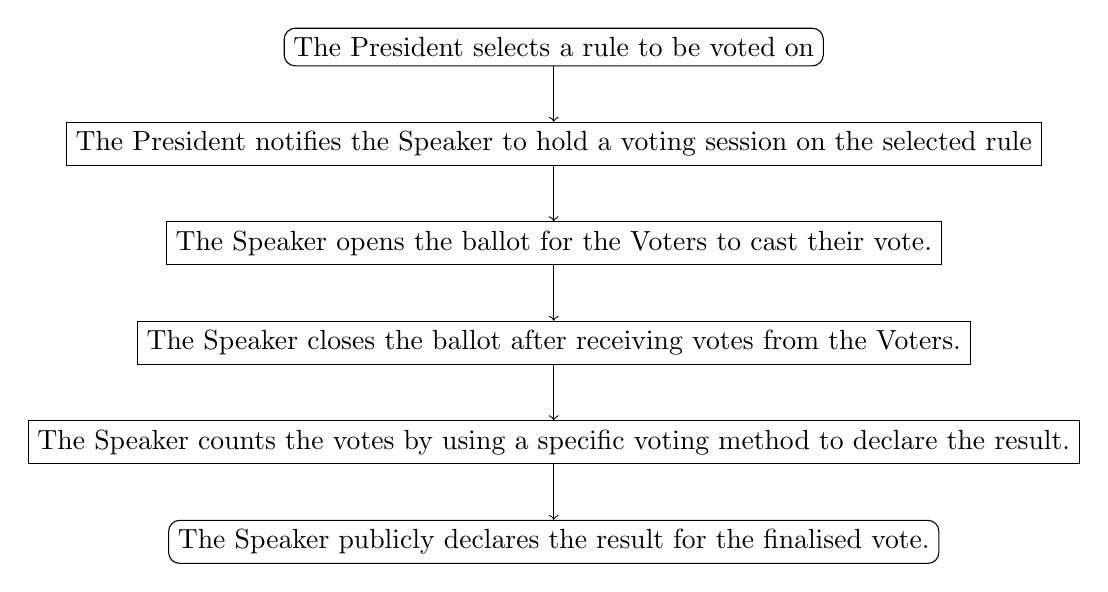
\begin{tikzpicture}[node distance=20pt]
\centering
\node[draw, rounded corners] (start)  {The President selects a rule to be voted on};
\node[draw, below=of start] (step 1)  {The President notifies the Speaker to hold a voting session on the selected rule};
\node[draw, below=of step 1] (step 2)  {The Speaker opens the ballot for the Voters to cast their vote.};
\node[draw, below=of step 2] (step 3)  {The Speaker closes the ballot after receiving votes from the Voters.};
\node[draw, below=of step 3] (step 4)  {The Speaker counts the votes by using a specific voting method to declare the result.};
\node[draw, below=of step 4, rounded corners] (end)   {The Speaker publicly declares the result for the finalised vote.};
 \draw[->] (start)  -- (step 1);
 \draw[->] (step 1) -- (step 2);
 \draw[->] (step 2) -- (step 3);
 \draw[->] (step 3) -- (step 4);
 \draw[->] (step 4) -- (end);
\end{tikzpicture}
\caption{Voting Protocol for Rules}
\label{fig:RONRVotingProtocol}
\end{center}
\end{figure}

For elections of roles, the sequence of actions of the voting protocol is mostly similar to the above explanation in principle, except for some parameters, such as the motion of the vote which is the role itself (President, or Speaker, or Judge), the facilitator of the election/vote event which depends on what role is being held for election (refer to Chapter 5 IIGO for more details on change of roles and power transfer), and the applicable voting method function to call for election that will produce the result, which is different from the voting method used for rules. Refer to Section~\ref{sec:VotingMethods} for more details on voting methods to be used for elections of roles.

At the start of the game, it is assumed that all 6 islands have the power to vote at any necessary voting scenario, and no diplomatic sanction is in place for any island. However, in the further turns of the game, some island(s) could lose their right to vote and/or not permitted to participate in a voting event due to the diplomatic sanction(s) in place. Refer to Chapter 5 IIGO for details on diplomatic sanction. In this case, the Speaker will open the ballots to the eligible islands only , i.e. those who are permitted to vote at a certain state of the game.

% Implmentaion section deleted
\begin{comment}
\section{Implementation}
\label{sec:Implementation}

\subsection{Voting for Rules}
\label{sec:VotingForRules}
The implementation of voting for rules from infrastructure point of view (file:\texttt{rulevote.go}) basically follows the sequence of voting protocol as described in Section~\ref{sec:VotingProtocol}. At initialisation, there are two defined structs (collection of data fields) that are used as parameters for functions inside the voting algorithm, such as \texttt{RuleVote} and \texttt{BallotBox}. The \texttt{RuleVote} struct consists of 3 variables, i.e. \texttt{ruleToVote} (string) that contains the rule that has been selected by the President to be voted on, \texttt{islandsToVote} (list of integers) that contains a list of \texttt{ClientID} which indicates all eligible islands that participate in the voting session, and \texttt{ballots} (list of boolean) that contains the vote of each respective eligible islands where it can indicate the vote for in-favour or against the proposed rule. The \texttt{BallotBox} struct consists of 2 integer variables that act as accumulators for the count of each possible vote: \texttt{VotesInFavour} and \texttt{VotesAgainst}.

According to Section~\ref{sec:VotingProtocol}, The Speaker firstly starts a voting session by calling \texttt{SetRule(rule)} function that contains the rule selected by The President to be voted on. Next, the Speaker sets all eligible islands that can participate/have the right to vote in the voting session at that state of the game by using \texttt{SetVotingIslands(clientIDs[])} function. After that, the Speaker opens the ballots to get the votes from all eligible islands by calling \texttt{GatherBallots(clientMap[ClientID])} function. Subsequently, the \texttt{GetBallotBox()} function is called by the Speaker to gather the ballots that already contain the votes counting of those who are in-favour or against the proposed rule. Finally, the votes counting is concluded by comparing the votes of those in-favour vs those against, and the in-favour votes win when the counting is greater than or equal to the against votes counting, as reflected in \texttt{CountVotesMajority()} function. The Speaker then uses this result to declare the result of this voting session in IIGO.

\subsection{Elections}
\label{subsec:Elections}
The elections for roles implementation can be seen in the file:\texttt{election.go}. At initialisation, there is a defined struct \texttt{Election} that contains 4 parameters, i.e. \texttt{roleToElect} that indicates which role is being voted on (President, or Speaker, or Judge), \texttt{votingMethod} that indicates the voting method being used for the election to determine the winner selection, \texttt{islandsToVote} that contains a list of \texttt{ClientID} which indicates all eligible islands that participate in the voting session, and \texttt{votes} that is a list that contains the order rank of preference of the candidates for the role from each eligible island who casts the vote.

The election session begins by calling the \texttt{ProposeElection(role,method)} function that depends on which role being voted on and which role has obligation to facilitate the election (refer to Chapter 5 IIGO on Change of Roles and Power Transfer sections), and the selected voting method to be used for this election (refer to Section~\ref{sec:VotingMethods} for details on voting methods and Subsection~\ref{subsec:VotingPseudo} for pseudo-code implementation). The election facilitator then opens ballots to all eligible islands to cast their votes by calling \texttt{OpenBallot(clientIDs[])} function. The \texttt{Vote(clientMap[ClientID])} function gathers all the ballots containing the votes from all eligible islands that are obtained from \texttt{GetVoteForElection(roleToElect)} function returned from each client/island code execution. After that, the election facilitator closes the ballots by using \texttt{CloseBallot()} function and it returns the result of the votes counting using the selected voting method by calling each respective voting method function. This result is used by the election facilitator to declare the winner for the elected role. By default, the voting method for election is Borda Count and the function is called \texttt{bordaCountResult()} where the algorithm follows through what are explained in Section~\ref{sec:VotingMethods} and Subsection~\ref{subsec:VotingPseudo} where the Borda scores will be calculated based on the order rank of preference of the candidates from each ballot. The other voting methods can be used for election and it is selected by the election facilitator.

\subsection{Voting Methods Implementation Pseudo-code}
\label{subsec:VotingPseudo}

\textbf{Plurality}
\newline
Call for Voting inputs (int:IslandID, str:"Aye", "Nay" or "Abstain")\\
\begin{algorithm}[H]
\ForEach{$ballot \in ballots $}{
    \If{$Aye$} {Count for $Aye ++ $}
    \If{$Nay$} {Count for $Nay ++ $}
}
\If{$Aye > Nay$}{\Return the Winner: $Aye$}
\Else{\Return the Winner: $Nay$}
\end{algorithm}

\ \newline \ \newline \ \newline
\textbf{Borda Count}
\newline
\begin{algorithm}[H]
\For{all ballot}{
    $numNotIn\gets N-ballot.length$\\
    $shareScore\gets 1+...+numNotIn$\\
    \For{i from 0 to N-1}{
    \If{i is in ballots} {$scores[i]\gets scores[i]+N-K+1$ }
    \Else {$scores[i]\gets scores[i]+shareScore/numsNotIn$ }
    }
}
Sort candidates by Borda scores\\
\Return the candidate with the highest score
\end{algorithm}

\ \newline \ \newline \ \newline
\textbf{Runoff}
\newline
\begin{algorithm}[H]
\For{All $ballot \in ballots $}{
    Select two candidates with most first-placed votes
}
\If{either already has a majority}{
\Return the majority one}
\Else{Each voter selects one candidate of the top 2\\
}
\Return the candidate with the most votes
\end{algorithm}

\ \newline \ \newline \ \newline
\textbf{Instant Runoff}
\newline
\begin{algorithm}[H]
\ForEach{$ballot \in ballots $}{
\For{i from 0 to N-1}{
\If{i is first choice}{$scores[i]\gets scores[i]+N-K+1$}
}
}
\If{candidate in ballots $>1$}{
Remove the candidate with the fewest first
choice votes from the ballots.\\
GOTO the top for next round of counting
}
\Else{\Return the candidate}
\end{algorithm} 

\ \newline \ \newline \ \newline
\textbf{Approval}\\
\begin{algorithm}[H]
\ForEach{$ballot \in ballots $}{
    \For{i from 0 to N-1}{
    \If{i is in ballot} {$scores[i]\gets scores[i]+1$ }
    }

}
Sort candidates by scores\\
\Return the candidate with highest score
\end{algorithm}
\end{comment}
    \chapter{Team 1 Agent Design}

\section{Core Idea}
Team 1 agent was designed around the idea that the agent wants the whole archipelago to survive. However, the agent does have different configurations to allow for some malicious behaviour in order to facilitate some interesting agent interactions.

\section{Emotional state}

The agent's behaviour is affected by what we have termed her \emph{emotional state}. This is governed by the agent's current resources in relation to the living cost.

\begin{table} [htb]
    \centering
    \begin{tabular}{|l|l|}
        \hline
        \textbf{Emotional State} & \textbf{Condition} \\
        \hline
        Happy & Default state \\
        \hline
        Anxious & Current resources under 5 times the living costs \\
        \hline
        Desperate & Agent in critical state \\
        \hline
    \end{tabular}
\end{table}


\section{Opinions on Islands}
As information and resource sharing between islands is possible, it is possible and desirable for the agent to form an opinion of other islands. This be used to gauge the accuracy of information from other islands as well as, potentially, deny resource sharing to islands deemed ``selfish''.

Initially, opinion on all islands is neutral. Over time, through IITO and IIGO, opinions on islands will change. This will affect behaviour in IITO, as well as IIGO voting. Note that positive values correspond to positive opinions while negative values correspond to negative opinions.

\section{IITO Gifts}
When team 1 agent receives a request for gifts, the agent will decide how much to offer depending on the agent's current emotional state and the opinion of that island.

\begin{table} [htb]
    \centering
    \begin{tabular}{|c|p{0.5\textwidth}|}
        \hline
        \textbf{Emotional State} & \textbf{How is IITO handled?} \\
        \hline
        Happy & Agent will give away resources that satisfies the requested amount. Up to a percent of available resources. \\
        \hline
        Anxious & Agent will give away a ratio of the requested amount and its current resources. \\
        \hline
        Desperate & Agent will refuse any gift requests that it receives. \\
        \hline
    \end{tabular}
\end{table}

During IITO, the agent's opinion of other islands is affected. For every gift received, the agent's opinion of the gift-giver increases. However, the agent's opinion of an island can decrease if that island promised a gift and did not fulfil it.

Moreover, if the agent's opinion of an island is very high, the agent can decide to give gifts disregarding the agent's own anxiety. On the other hand, if an opinion of an island is very low, the agent can decide to refuse to send a gift even though the agent is happy.

For increase survivability, team 1 agent will accept any gift offers that it receives.

\subsection{Future Work}
Team 1 agent currently has a very straightforward IITO strategy. Possible alteration to this strategy could include:
\begin{itemize}
    \item Being less susceptible to bribery. The agent should stop increasing the opinion of an island after receiving $X$ amount of continuous gifts.
    \item Stop handing out gifts to islands that are not in critical state.
    \item Being proactive in bribery. The agent will give non-requested gifts to the current president in hopes that this will reduce tax and increase resource allocation from the common pool.
\end{itemize}

\section{IIFO Disaster Prediction}
Disasters can happen deterministically or stochastically (see Chapter~\ref{sec: Disaster} for more information). For an agent, it is important to predict when a disaster occurs so that as much disaster damage is mitigated using the common pool.

When the game starts, the disaster prediction made by the agent is random. This prediction always has a confidence value of $0$. As more disasters occur, a history of disasters is built up. Using this history, the mean disaster position ($x$, $y$), magnitude and period is calculated. A confidence value is calculated along with the mean disaster metrics and shared along with the prediction.

% Add a footnote on website?  https://www.mathsisfun.com/data/confidence-interval.html
The confidence value is calculated by finding the ratio between margin of error and the mean value. The smaller the margin of error, the more confident the agent is in her prediction. Therefore, a difference between the mean value and the margin of error must also be calculated. The confidence interval equation is used to calculate the margin of error:

\begin{equation}
    \label{eq: Team1MarginOfError}
    \textsc{Error} = Z \dfrac{s}{\sqrt{n}}
\end{equation}

where $s$, $n$ and $Z$ are the standard deviation, size of array and confidence interval respectively.

Using the difference between the mean value ($\bar{x}$) and the margin of error and taking the ratio of this result over the mean will provide the agent with the confidence value.
\begin{equation}
    \textsc{Confidence Value} = \frac{\bar{x} - \textsc{Error}}{\bar{x}}
\end{equation}.

The agent maintains a \textbf{trust score} for every island \emph{including itself}. This is based on the accuracy of islands' prediction of time left to the disaster.

Sharing and obtaining other disaster information to and from other islands respectively can increase the survivability of the archipelago. As more disaster predictions are shared, a network of trust between team 1 agent and other islands is built.

\subsection{Future Work}
While team 1 agent has a satisfactory disaster prediction algorithm, it does not make use of this prediction or predictions from other islands in any meaningful way. This is primarily due to disaster prediction being one of the last features to be implemented and not enough time being available to complete it.

Nevertheless, here are some possible uses for the disaster prediction system.

\begin{itemize}
  \item \textbf{Tax policy} --- As president, the agent could choose to increase or decrease taxation depending on (predicted) time left to disaster.
  \item \textbf{Voting} --- A trustworthy island could make for a better president, speaker or judge, as they would be able to act according to imminent disasters.
  \item \textbf{Common pool contribution} --- Based on predicted disaster location the agent may increase or decrease her common pool contribution. If a disaster is expected to affect the agent significantly then she could choose to mitigate resource loss by contributing a large amount to the common pool, as the alternative would be losing more resources.
\end{itemize}

Finally, prediction accuracy could be improved by using the prediction of the most trustworthy island, whether that is the agent herself or not, or averaging the predictions of the most trustworthy islands.

\section{IIGO: President}

Following the agent's core idea, as the president, the agent will try to enlarge the common pool as well as redistribute wealth among the islands, in an attempt to ensure the survival of as many islands as possible. This is achieved through an aggressive, tiered tax policy as well as denying common pool allocation requests to the wealthier islands.

This policy had to be verified as it could be vulnerable to ``free-rider'' islands, who could avoid paying tax and still reap the benefits of disaster protection from a large common pool and ``bailout'' allocations when they are low on resources.

As a test of this, a simulation was set up with a variable number of lawful and free-rider islands in order to measure the stability of this policy.

Three tax evading islands (half of the islands) was found to be the limit at which this policy would lead to collapse of the IIGO and the common pool. This was deemed an acceptable limit as at least half of the other agent teams would obey tax policy, at least most of the time or with a small amount of evasion. The resource graphs for the cases of two and three tax evading islands can be seen in \autoref{fig:team1:two_invaders} and \autoref{fig:team1:three_invaders}.

\begin{figure}[H]
\centering
\includegraphics[width=0.9\textwidth]{09_team1_agentdesign/images/two_invaders}
\caption{Resource graph. Islands 5 and 6 are evading tax.}
\label{fig:team1:two_invaders}
\end{figure}

\begin{figure}[H]
\centering
\includegraphics[width=0.9\textwidth]{09_team1_agentdesign/images/three_invaders}
\caption{Resource graph. Islands 4 to 6 are evading tax.}
\label{fig:team1:three_invaders}
\end{figure}

Note here that collapse of IIGO (as in \autoref{fig:team1:three_invaders}, with three tax evaders) does not automatically imply collapse of the archipelago; the islands appeared to survive (and, in fact, thrive) even after the collapse of IIGO.\@ It was taken as an assumption that this was only due to the uniformity of strategies, and in the ``real'' simulation, with heterogeneous agents, collapse of IIGO would lead to collapse of the archipelago.



\section{Foraging}
Multiple foraging strategies were developed, initially by intuition and later by attempting to address the shortcomings of previous attempts. They were developed in order and aptly named:
\begin{itemize}
    \item Return on Investment (ROI)
    \item Regression
    \item Flip Forage
\end{itemize}


\subsection{Return on Investment (ROI) Foraging}%
\label{sec:forage-roi}

This first algorithm is based on repeating successful foraging behaviours in the past, whether those be by the agent herself or another agent.

For the first few turns (the exact amount is configurable) the agent will forage randomly.

The agent maintains a history of foraging decisions and outcomes, including those received from IIFO.\@ When it comes time to forage, this history is sorted by ROI, i.e.\ the ratio of profit to contribution. Decisions that resulted in a loss, had profit smaller than the living cost, or had a larger contribution than a (configurable) percentage of available resources, are filtered out.

\subsection{Regression Foraging}%
\label{sec:forage-regression}

This strategy tries to predict the ideal foraging decision, even if that exact decision was not made in the past. This is done using regression, which is used to find the decision with the highest expected reward.

The \emph{regression} strategy forages randomly in the initial turns and history is kept as in \nameref{sec:forage-roi}. To make a foraging decision, the history is split by foraged resource (fish or deer), and quadratic regression is performed on contribution versus reward for both resources. From this, a quadratic equation is formed. If the quadratic equation found is negative then the optimal contribution can be found by differentiation. If it is positive then a (large) value is chosen as contribution, as a higher contribution should simply lead to a higher reward.

\subsection{Flip Foraging}

This strategy chooses the least foraged resource from the last turn, according to IIFO-reported data. Contributed amount is proportional to the chosen resource's total ROI from last turn. This choice was made under the assumption that ROI is an indicator of the resource's ``condition''. If a resource only gives moderate rewards (proportionally to input) it means that it is probably over-used currently and as such agents should allow it to recover, by scaling down their foraging attempts or by switching foraging types.

\subsection{Comparison}

To compare the three strategies, simulations were run with six agents, two using \emph{ROI foraging}, two using \emph{regression foraging}, and two using \emph{flip foraging}. IIGO and IITO were also disabled in order to isolate the efficacy of foraging methods from other parts of the game. The simulation was run five times and the results averaged over the 5 games as well as the two agents following the same strategy.

\begin{figure}[H] 
\centering
\includegraphics[width=0.6\textwidth]{09_team1_agentdesign/images/mean_survival_turns}
\caption{Mean survival turns for different strategies.}
\label{fig:team1:mean_survival}
\end{figure} 

\begin{figure}[H] 
\centering
\includegraphics[width=0.6\textwidth]{09_team1_agentdesign/images/total_efficiency}
\caption{Average foraging efficiency}
\label{fig:team1:average_efficiency}
\end{figure} 

It is clear from \autoref{fig:team1:mean_survival} that the \emph{flip} foraging strategy dominates the other two in terms of overall effectiveness. However, it is interesting to note that, according to \autoref{fig:team1:average_efficiency}, the \emph{ROI} foraging method is almost as efficient as \emph{flip}, which raises the question of what causes the difference in their success. This difference could be attributed to one core issue with the \emph{ROI strategy}: ignoring the absolute value of rewards. The agent will happily settle for a profit of $11$ resources, if that was obtained with a contribution of $0.1$ resources (a profit of $110000\%$) over a profit $50$ resources for a contribution of $25$ (a measly $100\%$). This means that in the long run living costs overwhelm the \emph{ROI} agent. The \emph{flip} agent does not take expected profit into account and as such is unaffected by this.

\emph{Regression} appears to occupy a medium between \emph{flip} and \emph{ROI}, however it is much less consistent, as evidenced by the error bars in \autoref{fig:team1:mean_survival}, with \emph{regression} surviving for under 10 turns in some runs.

%%% Local Variables:
%%% mode: latex
%%% TeX-master: "../main"
%%% End:

    \chapter{Team 2 Agent Design}
\section{Overall Agent Strategy}

The overall strategy of our agent is based on a series of distinct, overlapping dilemmas. The agent operates on principles based on Evolutionary Economic Theory \footnote{https://www.cambridge.org/core/what-we-publish/elements/evolutionary-economics}. Game theory and the use of the Nash equilibrium also guided the development of the strategies implemented. The other top-level strategy which overlaps with several dilemmas is the social dilemma; this is when we quantify the relationship we have with other agents to produce trust and confidence levels. The interaction between the top-level strategies with all of the dilemmas is shown in Figure~\ref{fig: top level strategy}. The top-level strategy's implementation into each agent function and role is discussed in the following sections. 

\begin{figure}[!htb]
    \centering
    \subfigure[Top level strategy]{
        \centering
        \includegraphics[width=0.49\textwidth]{10_team2_agentdesign/images/strategies.png}
        \label{fig: top level strategy}    
    }
    \subfigure[Ceremonial-Instrumental dichotomy]{
        \centering
        \includegraphics[width=0.49\textwidth]{10_team2_agentdesign/images/dichotomy.png}
        \label{fig: dichotomy}
    }
\end{figure}

\subsection{Evolutionary Economic Theory}
The term Evolutionary Economic Theory was first coined by economist Thorstein Veblen \footnote{https://www.cambridge.org/core/what-we-publish/elements/evolutionary-economics}. Evolutionary Economic Theory proposes that economic processes evolve, and it rejects the assumptions of classical rational choice theory. From Evolutionary Economic Theory, we categorised agent behaviour into distinct groups \footnote{https://www.cambridge.org/core/what-we-publish/elements/evolutionary-economics}. These groups are an altruist, fair sharer, and free rider. These are explained in Table~\ref{tab:Evolutionary Economic Theory Agent classifications}.


\begin{table}[!htb]
    \caption{Evolutionary Economic Theory Agent classifications}
    \label{tab:Evolutionary Economic Theory Agent classifications}
    \begin{tabular}{|c|m{0.3\textwidth}|p{0.4\textwidth}|}
    \hline
    \textbf{Agent classification} & \textbf{Definition}  & \textbf{Examples within the game} \\ \hline
    Altruist  & More concerned about the welfare of the group than themselves  & \begin{tabular}[p{0.4\textwidth}]{@{}p{0.4\textwidth}@{}}-Contributes a surplus to the common pool\\ -Generous with gifts\end{tabular}                                                     \\ \hline
    Fair Sharer                   & Contributes enough to the group  to negate their negative impact on it & \begin{tabular}[p{0.4\textwidth}]{@{}p{0.4\textwidth}@{}}-Contributes the minimum necessary amount of resources \\ -Gift allocation is measured and reasonable\end{tabular}                          \\ \hline
    Free rider                    & More concerned with their individual welfare than the welfare of the group & \begin{tabular}[p{0.4\textwidth}]{@{}p{0.4\textwidth}@{}}-Will not contribute enough to the common pool \\ -Gift requests above their requirement \\ -Will not give out gifts\end{tabular} \\ \hline
\end{tabular}
\end{table}
    

The advantage of using this theory over rational choice theory from classical economics is that it accounts for the irrational decisions agents or humans make when dealing with economic decisions, such as deciding how much to contribute to a common pool. Humans have evolved to develop heuristics \footnote{\url{https://www.sciencedirect.com/topics/social-sciences/heuristics}} which are "rules of thumb" in order to make economic decisions quickly and when all information is not present. These heuristics are typically based on emotion and will often result in irrational decisions; an example of this would be brand loyalty. This is very relevant within the context of the game because there is a cost to large computations (decision making). Also, there is an information failure \footnote{\url{https://www.economicsonline.co.uk/Market_failures/Information_failure.html}} as the agents often do not know the threshold of the common pool and other vital game metrics. This information failure forces agents to use heuristics similar to those used by real people. An excellent example of a heuristic within this agent strategy is the level of trustworthiness decided within the social dilemma. If every agent was rational and all information was present in the game, there is no need to trust or distrust agents as they would maximize both their welfare and that of others.

Another primary reason for selecting this theory as the basis of our design is to explore the ceremonial-instrumental dichotomy\footnote{\url{https://www.jstor.org/stable/3486187?seq=3\#metadata_info_tab_contents}}. This dichotomy is best represented by the graph in figure \ref{fig: dichotomy} and shows the importance of the game's setup. Our agent is attempting to oppose this traditional response to instrumental and ceremonial societies. It would be interesting to change the game's ceremonial and instrumental values by changing the setup. While the current game infrastructure does not support this, it would be interesting to investigate the ceremonial-instrumental dichotomy by allowing islands to invest resources into developing their foraging technology to obtain higher returns. It would be interesting to investigate how this instrumental shift would change our agent's strategy and others' actions. This update in technology would replace the ceremonial institutional set up of the IIGO as it becomes redundant. Allowing islands to invest in technological advancement would add an extra dimension to the game as it evolves, and the importance of the IIGO and other instrumental components would shift.

\subsection{Evolutionary Economic Theory Implementation}
%explain how we use the information from the theory

Figure~\ref{fig:methods-of-play} shows the different states of our agent's different methods of play. At any point during the game, the state of our agent is determined only by the level of the Common Pool. Our agent's objective is to oppose the strategies employed by other agents to attain stability in the game. To determine the method of play of the other agents, we look at whether the Common Pool is, on average, increasing or decreasing. If the pool is being depleted, it can be assumed that the other agents act as free-riders on average. To counteract this, we act as an altruist (see section \ref{sec:Common Pool Dilemma Strategy} for more detail). The average pool level is used because individual agent strategies are irrelevant for the game's overall course. Within the game, we also do not always have access to individual agents' contributions, which would be needed to classify them individually. This makes the average level of the Common Pool the only viable parameter. 

Our simulations demonstrated that starting the game in a "free-rider" state resulted in optimal agent performance and did not negatively impact the course of the game overall.

The default state for the agent is to be a "fair sharer." The agent will move into altruist mode when the weighted average of the Common Pool has dropped drastically. The agent considers a weighted average to ensure that the agent does not panic after every disaster and over contribute. The most recent turns will also be weighed higher to determine the course of the game. When the Common Pool stops decreasing, the agent will move back to fair sharer mode. Similarly, if the pool's weighted average increases by a large factor, then our agent moves into a free-rider state.

\begin{figure}
    \centering
    \subfigure[Method of Play diagram]{
    \centering
        \includegraphics[width=0.4\textwidth]{10_team2_agentdesign/images/MethodofPlay.png}
        \label{fig:methods-of-play}
    }
    \subfigure[Social Classification Order]{
    \centering
    \includegraphics[width=0.4\textwidth]{10_team2_agentdesign/images/Social.png}
    \label{fig:social-order}
    }
\end{figure}



\subsection{Social Classification}
The agent forms an opinion on others depending on different situations. Initial testing suggested that another island's gift-giving behaviour does not necessarily correlate with their quality of predictions. Consequently, the trust of other agents is computed and stored separately for each situation. The agent uses the weighted average of past interactions with other agents to determine whether to trust them in each situation for future interactions. Using a weighted average to compute trust resulted in notably better agent performance. This is because the agent's trust in other agents considers all interactions with other agents while weighting recent interactions more heavily.

An integer value represents the agent's trust metric for each agent in each situation between 0 and 100, where 100 denotes full confidence and 0 a complete lack thereof. This value is used to compute the expected outcomes of situations. These are then compared with real events to update the agent's confidence in the other agents regarding this situation. For example, when the agent receives predictions from other islands, it computes the weighted average to check whether it trusts the island. Once a disaster occurs, the magnitude or timing of the disaster is compared with the other island's prediction. This reality is used to assess their behaviour and update the trust metric for that island relating to that situation. The list of different "situations" includes how an agent behaves in a role such as the President, Judge, Speaker, gift-giving, and disaster prediction. The overall structure of how the agent forms opinions on other islands is shown in Figure~\ref{fig:social-order}.

\section{Gift Giving and Receiving}
The agent must decide whether or not to respond to other agents' gift requests and how much to request from others through gifting. The implementation does not consider whether or not an agent is critical when requesting gifts and instead considers its current method of play and the trustworthiness of the requesting agent. Figure~\ref{fig: gifts} shows a decision tree for how the agent will allocate or request gifts, in which the agent splits up the gift request among the other agents to increase the likelihood of an agent allocating the gift.


\begin{figure}[!htb]
    \subfigure[Gift Giving and Receiving decision tree]{
        \centering
        \includegraphics[width=0.49\textwidth]{10_team2_agentdesign/images/gifts.png}
        \label{fig: gifts}
    }
    \subfigure[Common Pool Strategy]{
        \centering
        \includegraphics[width=0.49\textwidth]{10_team2_agentdesign/images/common_pool_strategy.png}
        \label{fig: common_pool_strategy}
    }
\end{figure}



Depending on the method of play, the agent will request more or fewer gifts. This is inversely proportional to the number of resources taken from the Common Pool. The agent obtains a larger proportion of its needed resources from gifting than the Common Pool in the altruist state. This is done to mitigate common pool depletion in the interest of the common good. In a Fair-Sharer state, the agent aims to obtain its resource target equally from gifts and the Common Pool. A minor surplus is also included in the resource target to ensure that the goal is met, given that gifts from other agents cannot be guaranteed. In a Free-Rider state, the agent takes the majority of its resources directly from the Common Pool but still requests gifts to build up its resources by taking advantage of relationships with other agents as well as a Common Pool surplus.

The \textbf{Gifts} social classification situation refers to both when an island requests a gift from our agent and when our agent requests a gift from that island. The balance between agent gift requests and responses is used as a basis for opinion formation on another agent. Other agents that fulfill the agent's requests are rewarded with higher trust. The agent's own gift requests tend to be small but are also proportional to its trust in each other agent. Every gift interaction is used to update the agent's trust in another island's gifting behaviour.

\section{Common Pool Dilemma Strategy} \label{sec:Common Pool Dilemma Strategy}
The Common Pool dilemma strategy can be split into two considerations. One consideration is the current method of play (altruist, fair sharer, and free-rider), and the other is the current game state. A decision tree showing the common pool strategy is shown in Figure~\ref{fig: common_pool_strategy}. These considerations decide whether and how much we contribute or take from the Common Pool.

\subsection{Method of play consideration} \label{ssec:Method of play consideration}
The primary consideration for giving to the Common Pool dilemma is the agent's current method of play. The agent's state is determined by the Common Pool level, as seen in Figure~\ref{fig:methods-of-play}. The agent's default state as a "fair sharer" contributes the average amount of other agents to the Common Pool. This is calculated by evaluating changes in the Common Pool level from the previous turn and averaging this quantity by dividing by the number of alive agents. If the Common Pool level decreases, the most recent Common pool increase is used to determine the amount given.

By using the average Common Pool contribution, the agent benefits from the forecasting of other agents. This benefit would arise should another agent have an advanced forecasting prediction that determines the Common Pool threshold and what is required to mitigate the effects of a disaster. In this case, the agent would then contribute a similar quantity of resources. This "herd-mentality" approach relies on the assumption that other agents make rational decisions. So if it is evident that other agents are acting irrationally, the agent deviates from this approach to an alternative state (to become either a free-rider or an altruist).

The agent is in an altruist state when the Common Pool is struggling, which often means that other agents act as free-riders. This is where the meta-strategy of Evolutionary Economic Theory comes into play. It is in the agent's interest to contribute much more to the Common Pool to alter the game's course in a positive direction and prevent the pool from being below the threshold when a disaster occurs. Therefore, the agent contributes more resources to enact this balance on the system. 
The altruist resource contribution is a larger factor of the weighted average contribution and can be tuned using the \emph{altruist factor} variable in the agent's configuration.

In a free-rider state, the Common Pool has a surplus, and the agent assumes other agents are on average operating as altruists. In this situation, the agent contributes less to the Common Pool and preserves resources to mitigate short and long-term risk. Contributing too much to the Common Pool no longer benefits the greater good, as these resources can still be used to forage and generate more resources. Therefore, the agent accumulates resources when others are too generous, allowing greater foraging investments and making it easier to help other agents if they struggle in the future.

The method of play also impacts how the agent decides to take from the Common Pool. After game state considerations are made, the agent adjusts how much it takes from the Common Pool according to its Agent State. Table~\ref{tab:Method of play common pool taking} outlines a summary of how the agent adjusts how much it takes and gives a justification for each action. The amount to take from the pool depends on how willing other agents are to contribute to the agent within the game's gift-giving section.  This means the agent must decide what proportion of the resource request must be taken from the Common Pool and from gifting, and this decision also factors in both common pool allocation as well as gift response predictions. When the agent is in a free-rider state, the common pool has a surplus, and so it makes more sense to take directly from the pool rather than requesting gifts. 

\begin{table}[!htb]
\centering
\caption{Method of play common pool taking}
\label{tab:Method of play common pool taking}
\begin{tabular}{|c|c|}
\hline
\textbf{Agent classification} & \textbf{How this impacts taking from the common pool}                              \\ \hline
Altruist                      & Pool is being depleted, best to not take from the pool                             \\ \hline
Fair Sharer                   & Gift requests and taking from the pool are equal                                   \\ \hline
Free rider                    & \multicolumn{1}{l|}{Pool has surplus, take from the pool rather than gift request} \\ \hline
\end{tabular}
\end{table}

\subsection{Game state consideration} \label{ssec:Game state consideration}
The primary consideration in taking from the Common Pool is the current game state. The key parameters (shown in Figure~\ref{fig: common_pool_strategy}) considered are whether the agent is critical and whether the agent has excess resources. This excess is calculated as the difference between the agent's current resources and the minimum resource threshold and the cost of living. Beyond this minimum resource level, the agent can survive one another turn. If the agent has fewer resources than these aggregated costs, the excess is zero. If there are excess resources, the agent will give some resources to the Common Pool. In this case, a strategic contribution is calculated. If the Common Pool threshold is known, the agent considers how many resources are required to attain this threshold. This is then spread over the expected number of turns until the next disaster is predicted to occur and the number of alive clients. If this is unknown, a default value is used to form an initial guess in the agent configuration. On top of this quantity, a strategic contribution is also calculated (see \ref{ssec:Method of play consideration}). The current method of play determines whether the disaster-determined contribution or the strategy-determined contribution is contributed to the pool. This amount is then contributed together with the current tax, unless there are no excess resources as this implies the agent is in a critical state and so all resources are preserved.

\section{Foraging Dilemma}
The foraging dilemma is split into two parts. One determines whether the agent should hunt or fish, and the other determines how many resources to spend on foraging. The foraging dilemma only depends on the current method of play. The method of play will impact the amount the agent uses to forages. If the Common Pool is doing well and the agent acts as a free rider, it will be more prone to take risk and contribute more to the foraging and vice versa. The decision to hunt or fish depends on the likely number of hunters in the next foraging event. The decision tree, Figure~\ref{fig: Hunt or fish decision tree }, shows how the agent decides whether to hunt or fish in a given turn. To determine the number of hunters in the next forage turn, the agent tracks how often each agent is a hunter and then sums up the probability of each agent hunting to find an overall number of likely hunters. The agent outputs a random number from 0 to 1, and if the number lies above the threshold, the agent will hunt. This threshold is determined by the number of likely hunters in the foraging. It implies there is an element of randomness to the agent's decision making, which will account for the unpredictability of dealing with other agents with their strategies.

\begin{figure}[!htb]
    \centering
    \subfigure[Hunt or fish decision tree]{
        \centering
        \includegraphics[width=0.4\textwidth]{10_team2_agentdesign/images/forage_decision.png}
        \label{fig: Hunt or fish decision tree }
    }
    \subfigure[Roles Decision Tree]{
        \centering
        \includegraphics[width=0.4\textwidth]{10_team2_agentdesign/images/Roles Decision Tree.png}
        \label{fig: Roles Decision Tree}
    }
    \caption{Hunting or Fishing and Roles Decision Tree}
\end{figure}



The ideal distribution for foraging is to have two agents hunting and the remainder fishing. Hence, when the agent predicts one other agent will hunt, the agent is highly likely to choose to hunt too. The default threshold for hunting is 0.1, so the agent will hunt 10\% of the time when not considering the likely number of hunters. By assuming that any agent will hunt or fish with equal probability, the likelihood that there is one hunter is approximately 0.16. This implies hunting is an optimal strategy approximately 16\% of the time, so a threshold similar to this value is chosen. If the predicted number of hunters is above one, the following equation is used to determine threshold placement: $\text{Probability of agent hunting} = 0.95 - \text{Predicted number of hunters} \times 0.15$

The probability of choosing to hunt when the agent is confident only one other agent will also select hunt is 0.95. For each additionally predicted hunter, the probability will fall by 0.15. This 0.95 threshold is included in the agent configuration so it can be edited without changing the code. Hence, the foraging decision can be tuned. The agent checks if there are any excess resources after considering the minimum resource threshold not to be critical and the cost of living. If there are no excess resources, no resources are spent on foraging. If there is an excess of resources, a percentage of this excess is used on foraging. This percentage is controlled in the agent configuration. This approach ensures the agent has enough resources to survive another round, even in the worst case scenario when foraging returns are minimal.

\section{Role Strategies}

Figure~\ref{fig: Roles Decision Tree} shows a decision tree of how the agent acts under the two roles implemented. Due to time constraints, the base client implementation was used for the Speaker. The President is responsible for allocating resources from the Common Pool based on agent requests. The agent uses game state variables such as their critical status to determine if another agent is worthy of their resource request and the agent's allocation method based on the method of play is outlined in Table~\ref{tab:President allocation method of play}. When the agent is in a free-rider state, it is more selfish, while when it is an altruist, more of the others agents requests are approved. If an agent is not critical, it is highly unlikely that the agent will allocate them their requested resources as the purpose of the Common Pool should be to primarily mitigate the effects of disasters. Resources are allocated on a need-first basis, taxed proportionally to an agents resource level, and the strategy to determine taxation includes an additional penalty tax for agents who do not declare their resource levels. When evaluating another President's performance, the agent considers the percentage change in tax, the percentage of how much the agent is allocated with respect to how much it requests, and how much the agent takes with respect to how much the President allocates it.

\begin{table}[!htb]
\centering
\caption{President allocation method of play}
\label{tab:President allocation method of play}
\begin{tabular}{|c|c|}
\hline
\textbf{Agent classification} & \textbf{\% of request given} \\ \hline
Altruist                      & 60                           \\ \hline
Fair Sharer                   & 50                           \\ \hline
Free rider                    & 40                           \\ \hline
\end{tabular}
\end{table}

The agent implementation of the Judge evaluates whether an agent has broken any rules, as it should. However, to model real world corruption, the agent does not sanction agents that break rules if it considers them to be highly trustworthy (i.e., with a trust score above 80\%). The agents behaviour as a Judge is also determined by its state; when the agent is a free-rider, it sanctions fewer islands. The \textbf{Judge}'s situation, similar to the President, is used by the agent to determine what island to vote for as Judge. This is done by checking the past sanctions the agent received and their duration, to maxmimise personal benefit. The \textbf{RoleOpinion} social classification situation is used when the agent is the Judge and must decide whether or not to pardon other islands' sanctions, whom to choose as the next President whether or not an island has adhered by the rules. The Judge receives information for each island, such as the difference between how much an island contributed to the common pool and how much said they would. The agent uses these differences as a Judge to determine whether or not an island is trustworthy. During a role election, the agent checks its trust in the candidates for the appropriate situation, i.e., the situation when an agent is "President" for a future Presidential election. The agent will return a list of candidates in decreasing order of preference determined by the social classification. To do this, the agent sorts the candidates in terms of how much it trusts them.

\section{Disaster Prediction}
It is important for the agent to be capable of predicting both the severity and timing of disasters, in order to effectively make decisions for contributing to both the common pool and gifting resources to other agents.

Since the simulation is constructed through a series of successive turns, the occurrence of disasters throughout the game can be seen as a Binomial distribution: $D \sim \text{Bin}(n,p)$. In this equation, $D$ describes the number of disasters that occur, $n$ is the number of turns played and $p$ is the probability of a disaster occurring on a given turn.

The aim of our agent is to estimate the number of turns between disasters. We will denote this random variable as $T_D$, with our agent's aim being to find $E[T_D]$. To do this, our agent must estimate $p$. Therefore we have programmed our agent to find the Maximum Likelihood Estimator of $p$ for a Binomial RV\footnote{https://stats.stackexchange.com/questions/191444/variance-in-estimating-p-for-a-binomial-distribution}: $\hat{p} = \frac{D}{n} = \bar{X}$, where $\bar{X}$ is the sample mean of the RV $X$. The expectation of $T_D$ can be estimated using\footnote{https://math.stackexchange.com/questions/1299465/proof-variance-of-geometric-distribution}: $\hat{\mu}_{T_D}= \frac{1}{\hat{p}} = \frac{1}{\bar{X}}$. Thus, this is the optimal estimator for our agent to predict the number of turns between disasters. Furthermore, the confidence that our agent has in this prediction should be inversely proportional to the variance of $T_D$, i.e. how much does $T_D$ vary from the expected value we have found above? The expression for this variance is given below$^2$: $Var(T_D)= \frac{1-p}{p^2}$. 

However, given that our agent does not know the actual value of $p$ used in the simulation, our agent instead estimates the variance using: $\hat{\sigma}_{T_D}^2= \frac{1-\hat{p}}{\hat{p}^2}$. Now that an expression for the estimate of this variance has been obtained, two questions remain: ``what about the variance in $\hat{p}$" and ``how is this variance translated into a confidence value?" The variance of $\hat{p}$ is given by the following expression: $Var(\hat{p})= Var(\bar{X}) = \frac{Var(X)}{n}$. As previously, we do not know the exact value of $p$, making a calculation of $Var(X)$ impossible. However, we can make use of the fact that $Var(\hat{p}) \propto \frac{1}{n}$, by making our agents confidence in the prediction proportional to $n$ also. Secondly, the fact that variance can take values $\in [0,\infty]$ but confidence must take a value $\in [0, 100]$ makes mapping the values of variance that our agent calculates, to a confidence level, challenging. The solution our team opted for was to cap the max value of variance to some value $v_{cap_{T_D}}$, before translating this variance into a corresponding confidence value. This process is given by the equation below: $\text{confidence}_{T_D} = 100 - \frac{100 \cdot \text{min}(\frac{\hat{\sigma}_{T_D}^2}{kn}, v_{cap_{T_D}})}{v_{cap_{T_D}}}$ 
where $k$ is the tuning parameter for altering the dependence of the confidence on $n$. 

\subsection{Magnitude Prediction}
Our agent's strategy for predicting the magnitude of the next disaster shares many similarities with the strategy discussed in the last section. However, the magnitude of the next disaster is now distributed with an Exponential distribution: $M \sim Exp(\lambda)$. Once again, start by finding the MLE for the parameter $\lambda$ \footnote{https://en.wikipedia.org/wiki/Exponential\_distribution}: $\hat{\lambda} = \frac{1}{\bar{M}}$. Now we seek to estimate the expectation of $M$: $\hat{\mu}_M = \frac{1}{\hat{\lambda}} = \bar{M}$. Similarly, the variance of this RV is also useful to estimate $\hat{\sigma}_{M}^2= \frac{1}{\hat{\lambda}^2}$. As previously, there is also a variance in our estimation of $\hat{\lambda}$ that must be taken into account by making our confidence in this prediction proportional to $n$. Thus, the following expression should be used for calculating the confidence in the magnitude prediction: $\text{confidence}_M = 100 - \frac{100 \cdot \text{min}(\frac{\hat{\sigma}_{M}^2}{gn}, v_{cap_M})}{v_{cap_M}}$, where $g$ is the tuning parameter for altering the dependence of the confidence on $n$. 

\subsection{Overall Prediction}
The overall prediction that must be shared with teams during the IIFO session requires the following information: location, time until next disaster, magnitude and confidence. For our prediction of location, the middle of the archipelago is always given since the probability of a disaster occurring at a given location is uniform across the archipelago, meaning that there is no optimal prediction formula. Using the findings presented in the above sections, the formulas our agent will use to form a prediction about the next disaster are as follows:

\begin{align*}
    &x_{coord} = x_{min} + \frac{(x_{max}-x_{min})}{2}, y_{coord} = y_{min} + \frac{(y_{max}-y_{min})}{2}, \text{conf} =\frac{\text{conf}_{T_D} + \text{conf}_M}{2} \\
    &\hat{\mu}_{T_D}=\frac{1}{\bar{X}}, \hat{\mu}_M = \bar{M} \\
\end{align*}

\subsection{Combined Prediction}
Generating our own prediction is only the first part of the prediction making process. The second stage is to make use of other island's predictions during the IIFO session and using the social classification to decide prediction accuracy. When considering how much emphasis to put on a given island's prediction, we make use of two factors: 1.) Our island's confidence in each other island's prediction making. 2.) Each island's confidence in their own prediction, $P_i \in [0,100]$. These two considerations are then combined to create an overall confidence factor.

\section{Simulations}
Every function and agent consideration has tuneable parameter which can be edited without changing the whole agent. Figure~\ref{fig: Forage Untuned} shows how our agent reacts when it plays against itself and the foraging parameters are untuned. As you can see the game is unstable and the agents have a low survival rate. This is caused by an over contribution to the foraging dilemma, there is a point of marginal return with the foraging dilemma and spending too many resources can be wasteful. 

\begin{figure}[!htb]
    \centering
    \includegraphics[width=0.6\textwidth]{10_team2_agentdesign/images/Forage Untuned.png}
    \caption{Untuned Forage Simulation}
    \label{fig: Forage Untuned}
\end{figure}

Figure~\ref{fig: Forage tuned} shows how our agents plays against itself when the foraging parameters are optimised. The amount of excess resources spent on foraging is more reasonable in this simulation, this results in a much higher survival rate and a more stable common pool.

\begin{figure}[!htb]
    \centering
    \includegraphics[width=0.6\textwidth]{10_team2_agentdesign/images/Forage tuned.png}
    \caption{Tuned Forage Simulation}
    \label{fig: Forage tuned}
\end{figure}

Figure~\ref{fig: altruist sim}  shows what happens when the agent plays itself and they are all altruists by default and do not move out of altruist. It can be seen that the agents over contribute to the Common Pool and are left with nothing to forage, this ends the game rather quickly. The simulation result was very similar for when all of the agents were free riders, the game would end in a couple of rounds after a lack of contribution to the common pool which caused impactful disasters.  This proves that being a free rider or altruist is not a rational decision and must be avoided. 

\begin{figure}[!htb]
    \centering
    \includegraphics[width=0.7\textwidth]{10_team2_agentdesign/images/altruist sim.png}
    \caption{Altruist simulation}
    \label{fig:  altruist sim}
\end{figure}
    % \newcommand{\subsubsubsection}[1]{\paragraph{#1}\mbox{}\newline}
% \setcounter{secnumdepth}{4}
% \setcounter{tocdepth}{4}


%TODO: Please DO NOT RESOLVE the comments unless you are 100% sure everything related to the comment is resolved, as they can't be retrieved.
%TODO: VERY VERY IMPORTANT: talk to people in our group to make a decision on understanding of the "lack of variety"  that is shown in the comment on line 276 of this latex file. This will cause quite a few changes in the report but it is a very important concept to clarify to avoid burning ourselves. Read all the comments Mike made in the relevant sections first.
%TODO: VERY IMPORTANT: another potential self burn area. Clarify with Rudolfs about Ostrom's Principles after looking at all the comments Mike has made in that section.
%TODO: add in rule distance calculation explanation? It's kinda primitive though
%DONE: President by Andrzej, do talk about disaster prediction
%DONE I THINK: Toby to finish all foraging related stuff (IIFO and End of turn)
%DONE: add in the use of disaster prediction somewhere if we can?
%DONE: to finish IITO and gifting, sneak in disaster prediction if possible - This is done except for the disaster prediction part. Not sure how to add it though, but feel free if you have an idea how.
%TODO: clear up all the TODO's scattered around in this latex file.


\chapter{Team 4 Agent Design}   \label{chap:team4}
Given that our team invested a significant amount of time in ensuring feature richness and stability of the infrastructure, we were left with a short time-frame for our agent's implementation and design. Therefore, at times we had to make decisions that guaranteed canny usability, rather than sophistication. For some actions, our agent relies on other teams' agents with different strengths to perform well. 

\section{Agent overview}
An agent uses the interface that is defined in the infrastructure. In order to define custom behaviours for our agent, we override or extend the base agent (\texttt{baseclient.go}) functions which implement the defined interface. The team built the agent design upon a set of internal fields that aid the decision-making process for the actions it performs. Information to describe the agent's personality is recorded in a structure of internal parameters, namely \texttt{Greediness}, \texttt{Selfishness}, \texttt{Fairness}, \texttt{Collaboration} and \texttt{RiskTaking}, all of which have decimal values between 0 and 1. The agent stores observations, histories as well as other necessary information such as its trust in others. These internal fields will be discussed in more detail in the following dedicated sections. %TODO: add in evolutionary economic theory background for agent personality

An agent can be elected in one or more positions of power inside the IIGO session, and be able to perform the duties of the office. From an infrastructure standpoint, these actions are implemented as overridable functions in the same fashion as previously discussed for the base agent. Although the code was design to differentiate a commoner agent and roles in separate structs, they all share read and write access to the internal fields of each other through pointers. In other words, an agent is always a commoner agent, and a commoner agent can be elected one or more role(s) at the same time.

\section{Opinion formation -- Trust}
\label{sec:team4:trust}
Trust is the score $[0..1]$, which represents the agent's opinion towards fellow agents in the game. This metric helps it in making decisions throughout the game based on how trustworthy, helpful or friendly it believes other agents were. This generic opinion about an island is formed dynamically based on three recurring observations:
\begin{itemize}
    \item The gifts received from the island during the IITO sessions.
    \item The outcome of monitoring positions-of-power when conducted as a part of the accountability cycle.
    \item The evaluation of IIGO actions history, only available to the Judge. This is further explained in Section \ref{subsec:team4:judge}
\end{itemize}
Those observations allow the agent to quantitatively reason about both friendliness of other islands towards it, as well as how closely they follow the rules in play.

The average trust score is forced at a value of $0.5$. Such normalisation ensures that the trust is always balanced throughout the game. It prevents the inflation of trust in a scenario where several islands decide to exchange gifts with the agent. Furthermore, the number of resources gifted will be a deciding factor when updating the trust metrics.

Some decisions made by our agent can be altered based on the trust score towards certain islands. During elections, if the trust of an island is lower than a specified threshold, the agent will never cast its vote in favour of it. Similarly, if holding the role of Judge, it will choose not to act upon its power to pardon the island with a low trust score.

On the other hand, if the agent holds a good opinion about an island, it may choose to favour it by providing or even deciding to  pardon it from a sanction.


\section{IIGO}
\subsection{Commoner Agent} \label{commoneragent}
At the start of any IIGO, each (commoner) agent is prompted by the president to report how many resources it has. Our agent overrides its reporting behavior  to account for several internal factors, as further discussed in subsection \ref{reportresources}. The president uses this information to set a taxation amount according to each agent's self-report, notifying them of the tax demanded. Each (commoner) agent can later send a request for the specific amount of resources it aims to retrieve from the Common Pool (an allocation request) to the President. Upon receiving a response from the President on the actual amount that was granted, the agent is allowed to access the Common Pool. The actions concerning requesting and taking allocations are overridden, as part of the agent strategy. Due to a design decision, the action for taking allocations and paying tax does not happen within the IIGO session, it happens after all organisations are run, inside the \texttt{EndOfTurn} session.

\subsubsection{Report Resources} \label{reportresources}
When reporting its resources, our agent uses a weighted linear combination of some of its internal fields. The weighting of each parameter is defined as an array of real values called "importance" and stored in an \texttt{importance} vector. The linear combination outputs a scaling factor to divide to the actual resources our agent has, as shown in \eqref{linear_comb}, in order to compute an untruthful amount to report to the President. The parameters used are \texttt{greediness}, \texttt{selfishness}, \texttt{fairness}, \texttt{collaboration}, \texttt{riskTaking} and trust in the current president (all values are between 0 and 1). Some fields are associated with negative weights as they should logically negatively impact the scaling factor. The greater the absolute value of weight, the bigger impact it has on the scaling factor.

\begin{equation}\label{linear_comb}
    \begin{bmatrix}
        w_{1}& w_{2}& w_{3}& w_{4}& w_{5}& w_{6}
    \end{bmatrix}
    \cdot
    \begin{bmatrix}
    Greediness \\ 
    Selfishness \\ 
    Fairness \\ 
    Collaboration \\ 
    RiskTaking \\
    TrustScore_{President}
    \end{bmatrix}
    = Scaling\:Factor
\end{equation}

To decide when to lie, the scaling factor is first compared to a preset threshold. If the scaling factor is greater, then the amount of the needed resource is divided by 
\begin{equation}
    [1 + (Scaling\:Factor - Preset\:Threshold)]
\end{equation} 
This conditional statement makes sure that the scaling factor is not always applied, ensuring that our agent will lie on its resources only when deemed a good strategy.

\subsubsection{Paying Tax Contribution}
%write about this and the lying mechanics
The \texttt{GetTaxContribution()} function returns the amount an agent is paying in tax. Similarly to resource reporting, the tax amount is modified by a scaling factor applied only when greater than a preset threshold, as shown in the following equation: 
\begin{equation}
    [1 + (Scaling \: Factor - Preset \: Threshold)]
\end{equation}
Based on the preset weighting for internal parameters, this situation is likely to arise when the \texttt{Collaboration} of our agent is high. In addition, the scaling factor is not applied when the tax demanded is more than $\frac{1}{5}$ of the agent's resources. This prevents it from generously giving out most that it has.

\subsubsection{Requesting Allocation}\label{subsubsection:CommonPoolResourceRequest()}

The aforementioned action of requesting resources from the common pool is implemented in the function: \texttt{CommonPoolResourceRequest()}. When requesting an allocation, our agent first decides what it needs. When not in a critical state, the needed resources are usually a multiple of the basic needs, namely the cost of living plus the critical threshold. This amount is decided so that the agent always takes more from the Common Pool than their definite expenses in the next turn. If critical, the agent will ask for a bigger multiple of the basic needs. This design choice maps the following logical conclusion that the agent draws from the history of the game: if the a smaller multiple when made the agent critical, it must take more to invert the negative trend in resources. In order to avoid draining the Common Pool, our design enforces that what our island needs must not exceed the number of resources in the Common Pool divided by the number of agents alive. This is to avoid our agent selfishly monopolising the Common Pool resources.

\subsection{President}
\label{subsec:team4:president}
Our agent implements a budget-conscious and rule-obeying President. The main changes, compared to the basic implementation include taxation and resource allocation considerations.

\subsubsection{Tax distribution}
When deciding tax amounts for the different island, the President considers the following variables:
\begin{itemize}
    \item amount of resources in the common pool
    \item the financial status of the island
    \item predicted disaster time and magnitude.
\end{itemize}

The President will abstain from setting taxation for islands in a critical state or in a situation when the resources in the common pool can fully mitigate the predicted damage caused by the next disaster. 

Similarly, when the common pool cannot mitigate the next disaster, the President will set taxation for all non-critical island to bring the common pool back to the safe level. In this case, the taxation amount will be higher the sooner the disaster is predicted to occur.

\subsubsection{Common pool resource redistribution}
In order to fairly redistribute the resources placed in the common pool, the President primarily considers the financial status of an island. In other words, the priority in access to the common pool is given to islands in the critical state. 

To ensure the largest possible satisfaction within the archipelago, the islands with smaller requests are given priority. This decision ensures that the highest possible number of agents will be satisfied with their allocation.

The President is also reluctant to allow any resource allocations if the disaster is predicted to occur soon. This, combined with the tax policy, ensures lower damages to the archipelago in the case of disaster.


\subsection{Judge}
\label{subsec:team4:judge}
The Judge implementation provided by our agent can be described as \emph{honest, but curious}. In other words, it follows the rules currently in play, and follows its obligations, however, it extracts the information exclusive to the Judge to reason about other agents in the game. An example of such actions is explained in greater detail below in this Section.

The judiciary functions overloaded from the \texttt{basejudge} implementation are:
\begin{itemize}
    \item \texttt{InspectHistory}, which examines rule violations of all the agents.
    \item \texttt{GetPardonedIslands}, which considers reducing the sanctions for some agents at judges discretion.
    \item \texttt{CallPresidentElection}, which initialises \emph{transfer-of-power} of the executive branch.
\end{itemize}
An explanation of the implementation of those functions is presented below.

\subsubsection{IIGO history inspection}
\label{subsubsec:team4:judge:inspect_history}
In the basic implementation, a history of IIGO actions of all the agents is passed to the Judge for inspection, which could become grounds for introducing economic sanctions for non-rule-obeying players. 

Judge truthfully evaluates and reports the rule violations for each of the agents, just as the \texttt{basejudge}. However, it also extracts and saves the information about the private resource pools of all the agents, taxes they were expected to pay, as well as the actual amount paid to the common pool. Additionally, it stores the \texttt{LawfulnessRatio} of each agent, which is defined as:


\begin{equation}
    lawfulness_{i} = \frac{number\:of\:rules\:obeyed\:by\:the\:agent_{i}}{total\:number\:of\:rules\:inspected\:by\:the\:judge\:for\:agent_{i}}
\end{equation}

where $agent_{i}$ denotes the $i^{th}$ agent in the game.  

The \texttt{LawfulnessRatio} is then used to update our agents' trust towards other islands, thus influencing decisions in different parts of the game. 

\subsubsection{Consideration of pardons}
Compared to the \texttt{basejudge}, which does not grant any pardons and requires islands to pay economic sanctions in full, our implementation of the Judge allows for the pardoning of certain islands. We consider three parameters when deciding whether and the island could be pardoned:

\begin{enumerate}
    \item The severity of the sanction - only sanctions lower than specified severity level can be considered to be pardoned. This ensures that our Judge never pardons an island, who notoriously breaks the rules of the game and gets sanctioned for it.
    \item Time served on the sanction - the Judge will only remove the sanction if at least the specified number of turns has been served by the island. This still allows us to have a punishment for not obeying the rules but also ensures that an island can begin to contribute again earlier.
    \item Trust towards the island sanctioned - only islands, which are considered trustworthy by our agent can be pardoned. The threshold is tuned by an internal parameter of our agent.
\end{enumerate}

An island can be pardoned by our implementation of Judge only if they meet all three requirements presented above. 


\subsubsection{Presidential elections}
The \texttt{basejudge} implementation called an election every three turns, no matter how long the presidential term was. Our Judge implementation improves on that by calling an election only under two conditions:
\begin{enumerate}
    \item The term of the president has ended.
    \item The president did not fulfil its obligations and was dishonest while holding the executive office. It is decided based on the monitoring results coming from the accountability cycle.
\end{enumerate}

This implementation could be further improved to facilitate the \emph{trust} metrics, explained in Section~\ref{sec:team4:trust}. An example of such an improvement would be allowing the president to hold the office longer than its turn if he is most trustworthy according to our internal \emph{trust} metrics.

\subsection{Speaker}
Given the Speaker's role of deciding agendas and announcing the results of the voting, the only viable customisation option in making our custom Speaker seemed to be implementing corruption - in other words, rigging voting results. Other than the obvious reason of avoiding the risk of getting sanctions, we decided against implementing this function into the Speaker's role because in an actual governmental environment, while misprints have occurred and on occasion shaped past history, announcing false results are a very noticeable and easily rectifiable offense. This would be in the disinterest of either honest or dishonest agents. On this note and the following point, it could be said that our Speaker implementation can be described as \emph{honorable and efficient}.

\subsubsection{Action prioritisation}

Our Speaker implementation builds upon the \texttt{baseSpeaker} on a key point: partitioning of budget. The Speaker prioritises the proper running of IIGO in the case of a low budget situation by prioritising its actions according to the rules in play, reflecting the priorities decided by the archipelago. This is done not by changing the actual running order of IIGO (which would require altering the orchestration) but rather enabling/disabling certain actions based on their priorities and cost. Prioritising actions where rules are in play would stop the speaker from performing non-moderated actions instead of actions relating to rules that are still in play. This function is crucial due to the following reasons:
\begin{itemize}
    \item Not performing monitored actions will result in sanctions, harming the agent's resource pool.
    \item The rules are a representation of the archipelago's expectations, thus not following said priorities is a sign of incompetence - damaging the agent's reputation.
\end{itemize}
Since these reasons are applicable regardless of honesty, these mechanics are always implemented regardless of the chosen personality type.

\section{IIFO}\label{sec:team4:IIFO}
%I recommend that we write in the order of function execution order. (the end of turn functions that are related to IIFO should be written inside the EndOfTurn section)Only mention the functions that are worth mentioning. For execution order check the ./doc/EXECUTION_ORDER.md file in the SOMAS repo -- Mike

\subsection{Making Disaster Prediction}
The agent makes predictions about future disasters by getting the mean coordinates, magnitude and number of turns per disaster (i.e. $\frac{1}{freq}$) from the previous disasters. It then computes a \texttt{confidence} score based on these mean values. The \texttt{confidence} score has a range between 0\% and 100\%. The sum of square of difference between the actual value and the mean value for each of the 4 prediction values types(coordinate x, coordinate y, magnitude and turns) is calculated as below:
\begin{equation}
    total = \sum_{i=1}^{len(past\_disasters)}(Value_i - Mean_i)^2
\end{equation}

The above is done for each of the 4 prediction values types. This returns a measurement of the distance between the predicted value (mean value) and the corresponding past disasters' values. The computed sum of square of difference (a measure of distance) is normalised with a max distance (see equations \ref{max_distance:1} to \ref{max_distance:3}) for each of the 4 value types, 100\% minus this percentage value is the \texttt{confidence} score. The \texttt{confidence} score for the prediction is the average of the 4 \texttt{confidence} scores.

Note that the Central Limit Theorem can be applied in this calculations since we assume different disasters are independent. Namely, the higher the distance between a prediction and samples, the less likely it is for this prediction to be true. And with the CLT assumption, the underlying random variables of the value types (uniform RV for coordinates, geometric RV for both magnitude and turns) do not matter. The calculation of the unique preset threshold is below:
\begin{equation}\label{max_distance:1}
    distance_1 = \sum_{i=1}^{len(past\_disasters)}(ValueMax - Mean_i)^2
\end{equation}
\begin{equation}\label{max_distance:2}
    distance_2 = \sum_{i=1}^{len(past\_disasters)}(ValueMin - Mean_i)^2
\end{equation}
\begin{equation}\label{max_distance:3}
    max\: distance = max (distance_1, distance_2)
\end{equation}

By doing the above unique threshold calculation for each value type, we are setting the predicted values out of bounds to have confidence 0\%. (Note: ValueMax and ValueMin are set in game config)

\subsubsection{Making prediction based on other agents' predictions}
Our agent then receives prediction information from all other agent that sent their information to us. A weighted average (based on trust) of these prediction values are calculated to form our final prediction values.

%Theoretically, We would use  a normal distribution to approximate the sampling distribution of the disaster random variable, which is assumed to be independent across turns, justified by the Central Limit Theorem. And by feeding  calculation approximated to be 


% Foraging functions %
\subsection{Sharing foraging information} \label{sec:team4:IIFO:forage}
IIFO also contains the ability to communicate about the foraging information. As we will go further into in Section~\ref{sec:team4:forage},
we choose to overload both MakeForageInfo and ReceiveForageInfo. In the receive function, we store the received values to a map to be used later when making a decision on which foraging method to go for. 

As we use the foraging information from other teams, our island will also communicate our results to the others. However, we only share with islands that shared with us in the previous round, as well as the island that we trust. Our island is completely truthful for this part and will always report which foraging method we went for, as well as how many resources it generated.

\subsection{IITO}
%(put and modify this to fit it somewhere in this section) If our agent is not in a critical state, it requests extra resources in addition to its own wanted resources in an intention to gift to other agents to earn their trust. If this allocation request is approved by the President, it proceeds with the gifting. These gifted resources are given on top of the normal gifts if there are any.
% some rough comments about IITO from Fabio: gifting pool is the key concept. same as president for allocation. Prioritise agents that are critical. Look at our selfishness and current resources. Help critical first(full amount no matter the trust). If not critical, only gift if trust > 0.5
In IITO we handle the process of sending, receiving, and requesting gifts.
Our island has an internal wealth goal which is calculated using our internal greediness and selflessness parameters. If our private pool is smaller than our wealth goal we ask for gifts from the other islands. The amount we ask for is related to the difference between the private pool and wealth goal. If we are in a critical state, however, we ask every island for two times the resources we estimate to be a safe resource level in the hope that at least one island will support us. 

When an island requests a gift from us we first check how many resources we can spare. This is once again calculated by taking the difference between the private pool and the wealth goal. We also look into its trustworthiness. If the island is critical, we prioritise that island. After that, we only return the gift relative to their trustworthiness. 
In addition, when we request allocation in IIGO, we request a bit extra which we gift to other islands in the hope that it will increase our reputation. This is only done if the president permits us to take the extra resources. 


 

\section{End of Turn}
\subsection{Taking Allocation}
This RequestAllocation() function for taking allocation from the Common Pool. After running all of the organisation sessions, the agent then calculates what it wants based on what it needs, and takes what it wants from the Common Pool. A scaling factor is calculated using a linear combination of weights and internal fields. When the scaling factor is above a preset threshold, it is applied similar to in Section~\ref{subsubsection:CommonPoolResourceRequest()}.  %talking about scaling factor calculation briefly, the detailed explanation is already done in ResourceReport. %%We use a linear combination of some of the agent's internal fields, and weights (put inside an \texttt{importance} vector) we set for each of the chosen internal fields to obtain a scaling factor to multiply the needed resources with. The parameters used are \texttt{greediness}, \texttt{selfishness}, \texttt{fairness}, \texttt{collaboration}, \texttt{riskTaking} and trust in the current president (all values are between 0 and 1). The weights have real values. For this particular function, we set the weights to be $5, 5, -5, -5, 1, 5$ respectively. The fields with negative weights negatively impact the scaling factor and vice versa. We deem riskTaking less important than other fields in the calculation of this function's scaling factor. The scaling factor is then compared to a preset threshold. If the scaling factor is greater, then the needed resources amount is multiplied by 1 plus the difference between the scaling factor and the preset threshold. The threshold is there to make sure that the scaling factor is not applied all the time, as we don't want our agent to take more than what it needs all the time.

\subsection{Forage} \label{sec:team4:forage}
As mentioned at the start of the chapter, due to the interest of time, our foraging strategy relies on other islands to make intelligent decisions about the foraging strategy. In short, rather than looking at the game configurations to try to intelligently figure out which method to go for and how many resources to generate, we look at other teams' return ratios to decide for ourselves. As will be discovered in the simulation section (\ref{sec:team4:simulation}), our foraging strategy works very well against the other islands created by the other teams, but not so well when we simulate six of our own islands.  

Our foraging strategy is split into two sections. Managing foraging communications is stored inside \texttt{IIFO.go} and our foraging decisions are stored inside \texttt{Foraging.go}.

As mentioned in Section~\ref{sec:team4:IIFO:forage}, 
the foraging is split into two parts, decision, and return. In the return, we store the results we receive into an array so that we can later use them in the decision making. This is also what we do inside IIFO when we receive the foraging results from the other teams. 

To decide whether to go fishing or to hunt deer the island looks at both its return history as well as looking at the return results received from the other teams. Our island does this is by calculating the return ratio of each island over the past three turns as well as our own. These ratios are then compounded into two separate values, the compounded ratio for deer hunting and the compounded ratio for fishing.  We then pick the foraging method that has the greatest compound ratio. 

How the island chooses to share its foraging results with other islands was described earlier in Section~\ref{sec:team4:IIFO:forage}. 


\section{Simulation}\label{sec:team4:simulation}


\subsection{Introduction}
Three different initial personality configurations were defined -
\emph{honest} , \emph{moderate} and \emph{dishonest} - in order to simulate how internal parameters would impact the agent's performance and interaction with the other teams.
These agents are designed to adapt their decision-making processes throughout the game, and each of these different personalities drew interesting hypotheses and observations about how a single agent would affect other agents and the system as a whole. This will be further discussed in Section~\ref{ResultSummary}. 

%TODO: add in evolutionary economic theory background for agent personality if we can explain it, it's a really good thing to add


The team decided to test both the interactions in the archipelago when populated by our clients with different personalities and the default clients developed by other teams (discussed in Section~\ref{againstothers} \nameref{againstothers}) as well as the interactions when only populated by instances of our client (discussed in Section~\ref{againstself} \nameref{againstself}). These simulation efforts have been made to investigate the effectiveness of the agent's strategy, the system's response to the lack of strategy variance, as well as the ability of the agents to react to this issue.

\subsection{Multi-agent simulations} \label{againstothers}
\subsubsection{Honest Client} \label{honestAO}
The \emph{honest} client has been carefully designed as an agent who would start the game complying to rules, offering help when possible and contributing to the common pool with more taxes when the agent is in abundant wealth. However, the personality of the agent adapts to the environment as it self-organises its strategy based on fellow agents. An irrefutable sign of great flexibility of this agent configuration is the presence of sanctions in its IIGO Report as shown in Figure~\ref{fig:IIGOHO}. The figure testifies that the agent adopts a change in strategy, occasionally breaking the rules. It still maintains a fair and collaborative approach throughout the whole game, getting involved in transactions during the IITO (Figure~\ref{fig:TransactionsHO}) and contributing to the common pool. 

As shown in the Resources Plot in Figure~\ref{fig:ResourcesHO} , where the agent is represented by the cyan curve, more than once there is a peak in resources that steeply decreases on the following turn. This happens because the agent is generously providing gifts to the agents in need and sometimes is also paying slightly more taxes into the common pool than required. From a design standpoint the team opted for an implementation that would prioritise gifts over over-contributions to the common pool. This decision comes from the consideration that a dishonest agent would counter our efforts in distributing resources to fellow agents. Therefore, prioritising gifting avoids this problem by allowing our agent to deliberately allocate its resources surplus to other islands. The agent acts even more magnanimously with islands in a critical state. This behaviour is clearly noticeable in disaster recovery.
\begin{figure}[H]
\centering
\includegraphics[scale=0.6]{12_team4_agentdesign/images/IIGOHO.PNG}
\caption{IIGO Payments For Honest Client Versus Other Teams.}
\label{fig:IIGOHO}
\end{figure}

\begin{figure}[H]
\centering
\includegraphics[scale=0.4]{12_team4_agentdesign/images/TransactionsHO.png}
\caption{Transactions For Honest Client Versus Other Teams.}
\label{fig:TransactionsHO}
\end{figure}
\begin{figure}[H]
\centering
\includegraphics[scale=0.7]{12_team4_agentdesign/images/ResourcesHO.PNG}
\caption{Resources Plot For Honest Client Versus Other Teams.}
\label{fig:ResourcesHO}
\end{figure}

\subsubsection{Moderate Client} \label{moderateAO}
The \emph{moderate} client is configured specifically to start the game with an internal set of parameters that would allow it to score values as close as possible to thresholds in each decision making matrix calculation. The team opted for such a design choice in order to maximise the agent's response time to the environment, making it much more flexible than its two counterparts, who take a longer time to modify their strategy. As a Moderate client was simulated against other teams, the team noticed that it would perform very similarly as the Honest agent, as the other teams were always run on a "honest-like" configuration. Similarly, it would quickly turn its behaviour to dishonest when running against dishonest-like implementations of other teams' agents.

\subsubsection{Dishonest Client}
The \emph{dishonest} client, aptly named, is designed to take advantage of a large amount of common resources without collaborating with others and systematically abusing positions of power to gain economical advantages. The yielded results highlighted an interesting behaviour of the system and of other agents. As per design, the system can only incentivise avoidance of such radical and rogue behaviour, resulting in a complete dominance of the dishonest agent. The agent proceeds to appropriate of all resources from the common pool and mercilessly watch other islands die, as profiled in the Figure \ref{fig:ResourcesDO}. Eventually, unable to survive without the collective help to mitigate disasters, dishonest agent slowly meets its demise. The other agents do not reach a level of understanding of the game that allows them to comprehend the changes in game state, adapt to them, and mitigate them by enforcing more severe rules. It must also be said that the system itself does not allow any hard enforcement, making it impossible for other agents to counter-attack a fully dishonest and selfish strategy, which disregards sanctions and taxes. 

Given these findings, dishonesty might seem like a dominant strategy as the agent survives the longest, securing all resources for itself. However, the long term dilemma imposes that islands must collaborate to survive for long periods. The dominance of this strategy is further refuted by the simulations performed in subsection \ref{dishonestAD}.

\begin{figure}[H]
\centering
\includegraphics[scale=0.4]{12_team4_agentdesign/images/ResourcesDO.png}
\caption{Resources Plot For Dishonest Client Versus Other Teams.}
\label{fig:ResourcesDO}
\end{figure}

\subsection{Uni-Agent Simulations} \label{againstself}
There are observations to be made from simulating our agent against instances of itself. The main issue identified can be referred to as a \emph{lack of variety}, which encompasses the problem of populating the archipelago with islands that share the same "mindset"; therefore, approach dilemma from a unified perspective. This hypothesis was raised as an attempt to explain the poor results of uni-client simulations which have been observed not only when running team 4 agents against themselves.

In all uni-agent simulations, the common pool was initialised to 1,000 resources, so that the agents could have enough resources to initialise running IIGO sessions.

\subsubsection{Honest Agents Only}
Populating the game with only honest clients provided a starting environment where all clients in the game are inclined to obey to rules and contribute a lot to the common pool in collective efforts. From this standpoint it makes sense that clients would build strong relations of trust and retain a high opinion of each other, as they treat each other with a fair and collaborative personality. Therefore in the evolution of the game, no agent undertakes any radical change of personality as was the case when our honest client was placed against other teams in subsection \ref{honestAO}. The IIGO Payments histogram in Figure \ref{fig:IIGOHH} nicely shows how the islands do not break any rule throughout the entire run.

It also manifests a very predictable behaviour of each honest agent that is perfectly in line with their design, such as paying more taxes than requested and taking less allocations than granted. We identified this predictable behaviour as an example of \emph{lack of variety} that shows how agents with the same specification do not have strengths in all aspects of the system to survive in such a complex system that needs to be properly discovered and efficiently exploited.

\begin{figure}[H]
\centering
\includegraphics[scale=0.8]{12_team4_agentdesign/images/IIGOHH.png}
\caption{IIGO Payments For Honest Clients Only.}
\label{fig:IIGOHH}
\end{figure}

\subsubsection{Moderate Agents Only}
As presented in subsection \ref{moderateAO}, moderate agents are specifically designed to increase the variance in agent strategy. As a result, the \emph{lack of variety} issue should have been mitigated in a simulation where moderate agents face each other. After running the simulations, the clients have indeed acted far less predictably. Comparing Figure \ref{fig:IIGOMM} with the histogram plot shown in Figure \ref{fig:IIGOHH}, the breadth of a larger variety of game strategies can be observed. Namely, agent 2 and 3 show more dishonest traits, hence getting sanctions for performing illegal actions. Meanwhile, other clients take a more honest approach which replicates the ones observed by the honest clients. For other clients, like number 6, this honest strategy is less pronounced.

\begin{figure}[H]
\centering
\includegraphics[scale=0.8]{12_team4_agentdesign/images/IIGOMM.png}
\caption{IIGO Payments For Moderate Clients Only.}
\label{fig:IIGOMM}
\end{figure}

Although the variance of agents strategy is significantly higher, clients still share the same underlying "mindset". This means that they define their whole personality using the same features, such as approaching tasks like foraging and power roles in the same way. Therefore, although the simulations ran show a slight improvement compared to "only honest" and "only dishonest" studies, they are far from producing a successful game like in multi-agent simulations. One of the main causes of this phenomenon was identified as the poor performance of actions that have been deliberately implemented in a simpler way in order to reduce the complexity of the agent. In particular, a foraging strategy in a well-performing multi-agent system may be to just replicate the foraging decision of the team that is economically strongest. However, in a uni-agent environment, this strategy  results in a group of agents mutually trusting their foraging strategy where nobody considers which one is actually the most profitable given the current circumstances.

Furthermore, features such as proposing rules is another good example of how lacking variety results in weaker archipelagos. This action enhances the ability of clients to adapt to the environment, crafting new rules as unexpected situations arise. If a client decides not to implement this feature in a multi-agent system, its effect on the adaptive capability of the archipelago will be almost fully mitigated by more complex clients that do perform such action.

\subsubsection{Dishonest Agents Only} \label{dishonestAD}
The last pure uni-agent simulation shows how dishonest clients face each other. This is, by far, the setting in which island longevity suffers the most as all clients start off the game with the intent to take advantage of the full resources with no compassion for others - demonstrating that with uncurbed dishonest agents, the system and agents cannot sustain the game. Runs in this environment feature one of the island who wins the race and empties the common pool, leaving other islands to die. The whole demise is made even faster by the total lack of collaboration among agents. Figure \ref{fig:ResourcesDD} demonstrates just how fast the archipelago is decimated. This comes as an additional proof of the fact that dishonesty cannot be considered a dominant strategy, as it doesn't perform better than all other strategies of the agent no matter what strategy the other agents choose. Indeed an honest or moderate client in such a setting would perform significantly better.
\begin{figure}[H]
\centering
\includegraphics[scale=0.8]{12_team4_agentdesign/images/ResourcesDD.png}
\caption{Resources for Dishonest Clients Only.}
\label{fig:ResourcesDD}
\end{figure}

\subsubsection{Mixed Agents}
In an attempt to overcome the \emph{lack of variety} problem, simulations were run by instantiating two clients from each personality to promote variance. As demonstrated in Figure \ref{fig:IITOTransMA} via the “transactions” and “IITO” plots, the honest and moderate islands dominate in contributing to the community and share resources compared to the two dishonest clients “5 and 6”. Despite the clear difference in approaches from interaction plots, the game is still destined to finish early - failing to over come \emph{lack of variety}. This may be because agents are still sharing the same underlying “mindset” as they take decisions based on the same thresholds. They also are structured in the same way, so specific strategies like foraging or optional actions like proposing rules, if they are not implemented at all or just heavily relying on other clients making smart choices, will not work as well as in a more diverse environment.

\begin{figure}[H]
\centering
\begin{minipage}{.5\textwidth}
  \centering
  \includegraphics[width=.45\linewidth]{12_team4_agentdesign/images/IITOMA.png}
  IITO interactions
  %\captionof{IITO interactions}
\end{minipage}%
\begin{minipage}{.5\textwidth}
  \centering
  \includegraphics[width=.45\linewidth]{12_team4_agentdesign/images/TransactionsMA.png}
  Transactions
  %\captionof{Transactions}
\end{minipage}
  \label{fig:IITOTransMA}
  \caption{IITO interactions and transactions among mixed clients.}
\end{figure}


\subsection{Results Summary} \label{ResultSummary}
%Rudolfs suggestion on phrasing it as experts in the field allow all islands to thrive.%
\subsubsection{Lack of variety}
The \emph{lack of variety} problem was a reoccurring trend in all our uni-agent simulations. The question comes in when considering whether or not this trend was avoidable or not. Because our agents while having strengths in specific areas, had obvious weaknesses when it comes to rule proposal, putting the same agent up against each other resulted in a stalemate due to the lack of coverage of the game's functionalities. This could be a problem with agents that do not have a high level understanding of the whole game.

This begs the question on whether an optimal strategy would even exist on a game such as this if all participating agents have the same level of complexity. A possible solution to this may be to have a more advanced state machine, an agent design our team has considered on the developing stages. The core concept is that an agent can have a higher level of understanding of the situation the agent is put in. This indicates that in order to overcome the \emph{lack of variety} problem, it is not enough to have flexible thresholds and parameters, which are more tactical measures - the agent's design approach itself must be radically different at each state. This would require a lot of rewritten and well-partitioned code which was not sufficiently form-able in our limited time frame.

\subsubsection{Agent-institution interaction}

Evident by the behaviour of the dishonest agents, even with IIGO present, it is still possible to completely drain the common pool from any resources. As examined in the evaluation of IIGO, there are areas of power within IIGO which are not governed by institutional design. One of these is a lack of a Zone of Dignity, or similar solution, for the decisions on how much the agents should request in allocations and how much the President can allocate. In the current implementation there are no rules stating that the agent is not permitted to request resource amounts above some threshold. Moreover, there are no "guardrails" the President has to follow when allocating these resources. Thus a greedy agent, like the one we implemented, in combination with a generous President results in disastrous situations since the common pool stays permanently empty. There is no disaster mitigation and thus no source, besides presents, to reach for help in the case of critical financial status. Hence, a better approach to a dishonest agent in the current IIGO setting would be to keep all other agents minimally satisfied.

A more notable result is the one we see in regard to Ostrom's third principle. In the limited time our agent was developed in, it relies on the strategy of others for its own survival. The presence of other "expert" agents can aid in the survival of less developed ones. This is in line with the assumption behind opinion formation and voting. By allowing the agents to rely on the strategy of others, for example, relying on good disaster prediction algorithm from another agent, agents can disregard those aspects as long as they are satisfied with the work of the "experts". Similarly, our agent relies on the rule proposal of others to function. When there is a lack of experts and an agent lacks the ability to fill the institutional gaps in that field, that area of the institution collapses. This is also known as the problem students face when first coming to university and realising they have little expertise in cooking. 

One way to solve our agent's lack of expertise in rule proposal would be to make the agent spontaneously create rules or create all possible rules based on its understanding of the situation of the game. This requires effective collection of all useful information from the game, as well as successful interpretation of the information. In addition, the agent would need to predict the how rules interact with each other and what rules it desires in the short versus long term. A machine learning approach might be a good solution for this problem. The task is not trivial even for humans, however even sub-optimal solutions could benefit the agents ability to survive and interact with the institution.
    % \newcommand{\subsubsubsection}[1]{\paragraph{#1}\mbox{}\newline}
% \setcounter{secnumdepth}{4}
% \setcounter{tocdepth}{4}


%TODO: Please DO NOT RESOLVE the comments unless you are 100% sure everything related to the comment is resolved, as they can't be retrieved.
%TODO: VERY VERY IMPORTANT: talk to people in our group to make a decision on understanding of the "lack of variety"  that is shown in the comment on line 276 of this latex file. This will cause quite a few changes in the report but it is a very important concept to clarify to avoid burning ourselves. Read all the comments Mike made in the relevant sections first.
%TODO: VERY IMPORTANT: another potential self burn area. Clarify with Rudolfs about Ostrom's Principles after looking at all the comments Mike has made in that section.
%TODO: add in rule distance calculation explanation? It's kinda primitive though
%DONE: President by Andrzej, do talk about disaster prediction
%DONE I THINK: Toby to finish all foraging related stuff (IIFO and End of turn)
%DONE: add in the use of disaster prediction somewhere if we can?
%DONE: to finish IITO and gifting, sneak in disaster prediction if possible - This is done except for the disaster prediction part. Not sure how to add it though, but feel free if you have an idea how.
%TODO: clear up all the TODO's scattered around in this latex file.


\chapter{Team 4 Agent Design}   \label{chap:team4}
Given that our team invested a significant amount of time in ensuring feature richness and stability of the infrastructure, we were left with a short time-frame for our agent's implementation and design. Therefore, at times we had to make decisions that guaranteed canny usability, rather than sophistication. For some actions, our agent relies on other teams' agents with different strengths to perform well. 

\section{Agent overview}
An agent uses the interface that is defined in the infrastructure. In order to define custom behaviours for our agent, we override or extend the base agent (\texttt{baseclient.go}) functions which implement the defined interface. The team built the agent design upon a set of internal fields that aid the decision-making process for the actions it performs. Information to describe the agent's personality is recorded in a structure of internal parameters, namely \texttt{Greediness}, \texttt{Selfishness}, \texttt{Fairness}, \texttt{Collaboration} and \texttt{RiskTaking}, all of which have decimal values between 0 and 1. The agent stores observations, histories as well as other necessary information such as its trust in others. These internal fields will be discussed in more detail in the following dedicated sections. %TODO: add in evolutionary economic theory background for agent personality

An agent can be elected in one or more positions of power inside the IIGO session, and be able to perform the duties of the office. From an infrastructure standpoint, these actions are implemented as overridable functions in the same fashion as previously discussed for the base agent. Although the code was design to differentiate a commoner agent and roles in separate structs, they all share read and write access to the internal fields of each other through pointers. In other words, an agent is always a commoner agent, and a commoner agent can be elected one or more role(s) at the same time.

\section{Opinion formation -- Trust}
\label{sec:team4:trust}
Trust is the score $[0..1]$, which represents the agent's opinion towards fellow agents in the game. This metric helps it in making decisions throughout the game based on how trustworthy, helpful or friendly it believes other agents were. This generic opinion about an island is formed dynamically based on three recurring observations:
\begin{itemize}
    \item The gifts received from the island during the IITO sessions.
    \item The outcome of monitoring positions-of-power when conducted as a part of the accountability cycle.
    \item The evaluation of IIGO actions history, only available to the Judge. This is further explained in Section \ref{subsec:team4:judge}
\end{itemize}
Those observations allow the agent to quantitatively reason about both friendliness of other islands towards it, as well as how closely they follow the rules in play.

The average trust score is forced at a value of $0.5$. Such normalisation ensures that the trust is always balanced throughout the game. It prevents the inflation of trust in a scenario where several islands decide to exchange gifts with the agent. Furthermore, the number of resources gifted will be a deciding factor when updating the trust metrics.

Some decisions made by our agent can be altered based on the trust score towards certain islands. During elections, if the trust of an island is lower than a specified threshold, the agent will never cast its vote in favour of it. Similarly, if holding the role of Judge, it will choose not to act upon its power to pardon the island with a low trust score.

On the other hand, if the agent holds a good opinion about an island, it may choose to favour it by providing or even deciding to  pardon it from a sanction.


\section{IIGO}
\subsection{Commoner Agent} \label{commoneragent}
At the start of any IIGO, each (commoner) agent is prompted by the president to report how many resources it has. Our agent overrides its reporting behavior  to account for several internal factors, as further discussed in subsection \ref{reportresources}. The president uses this information to set a taxation amount according to each agent's self-report, notifying them of the tax demanded. Each (commoner) agent can later send a request for the specific amount of resources it aims to retrieve from the Common Pool (an allocation request) to the President. Upon receiving a response from the President on the actual amount that was granted, the agent is allowed to access the Common Pool. The actions concerning requesting and taking allocations are overridden, as part of the agent strategy. Due to a design decision, the action for taking allocations and paying tax does not happen within the IIGO session, it happens after all organisations are run, inside the \texttt{EndOfTurn} session.

\subsubsection{Report Resources} \label{reportresources}
When reporting its resources, our agent uses a weighted linear combination of some of its internal fields. The weighting of each parameter is defined as an array of real values called "importance" and stored in an \texttt{importance} vector. The linear combination outputs a scaling factor to divide to the actual resources our agent has, as shown in \eqref{linear_comb}, in order to compute an untruthful amount to report to the President. The parameters used are \texttt{greediness}, \texttt{selfishness}, \texttt{fairness}, \texttt{collaboration}, \texttt{riskTaking} and trust in the current president (all values are between 0 and 1). Some fields are associated with negative weights as they should logically negatively impact the scaling factor. The greater the absolute value of weight, the bigger impact it has on the scaling factor.

\begin{equation}\label{linear_comb}
    \begin{bmatrix}
        w_{1}& w_{2}& w_{3}& w_{4}& w_{5}& w_{6}
    \end{bmatrix}
    \cdot
    \begin{bmatrix}
    Greediness \\ 
    Selfishness \\ 
    Fairness \\ 
    Collaboration \\ 
    RiskTaking \\
    TrustScore_{President}
    \end{bmatrix}
    = Scaling\:Factor
\end{equation}

To decide when to lie, the scaling factor is first compared to a preset threshold. If the scaling factor is greater, then the amount of the needed resource is divided by 
\begin{equation}
    [1 + (Scaling\:Factor - Preset\:Threshold)]
\end{equation} 
This conditional statement makes sure that the scaling factor is not always applied, ensuring that our agent will lie on its resources only when deemed a good strategy.

\subsubsection{Paying Tax Contribution}
%write about this and the lying mechanics
The \texttt{GetTaxContribution()} function returns the amount an agent is paying in tax. Similarly to resource reporting, the tax amount is modified by a scaling factor applied only when greater than a preset threshold, as shown in the following equation: 
\begin{equation}
    [1 + (Scaling \: Factor - Preset \: Threshold)]
\end{equation}
Based on the preset weighting for internal parameters, this situation is likely to arise when the \texttt{Collaboration} of our agent is high. In addition, the scaling factor is not applied when the tax demanded is more than $\frac{1}{5}$ of the agent's resources. This prevents it from generously giving out most that it has.

\subsubsection{Requesting Allocation}\label{subsubsection:CommonPoolResourceRequest()}

The aforementioned action of requesting resources from the common pool is implemented in the function: \texttt{CommonPoolResourceRequest()}. When requesting an allocation, our agent first decides what it needs. When not in a critical state, the needed resources are usually a multiple of the basic needs, namely the cost of living plus the critical threshold. This amount is decided so that the agent always takes more from the Common Pool than their definite expenses in the next turn. If critical, the agent will ask for a bigger multiple of the basic needs. This design choice maps the following logical conclusion that the agent draws from the history of the game: if the a smaller multiple when made the agent critical, it must take more to invert the negative trend in resources. In order to avoid draining the Common Pool, our design enforces that what our island needs must not exceed the number of resources in the Common Pool divided by the number of agents alive. This is to avoid our agent selfishly monopolising the Common Pool resources.

\subsection{President}
\label{subsec:team4:president}
Our agent implements a budget-conscious and rule-obeying President. The main changes, compared to the basic implementation include taxation and resource allocation considerations.

\subsubsection{Tax distribution}
When deciding tax amounts for the different island, the President considers the following variables:
\begin{itemize}
    \item amount of resources in the common pool
    \item the financial status of the island
    \item predicted disaster time and magnitude.
\end{itemize}

The President will abstain from setting taxation for islands in a critical state or in a situation when the resources in the common pool can fully mitigate the predicted damage caused by the next disaster. 

Similarly, when the common pool cannot mitigate the next disaster, the President will set taxation for all non-critical island to bring the common pool back to the safe level. In this case, the taxation amount will be higher the sooner the disaster is predicted to occur.

\subsubsection{Common pool resource redistribution}
In order to fairly redistribute the resources placed in the common pool, the President primarily considers the financial status of an island. In other words, the priority in access to the common pool is given to islands in the critical state. 

To ensure the largest possible satisfaction within the archipelago, the islands with smaller requests are given priority. This decision ensures that the highest possible number of agents will be satisfied with their allocation.

The President is also reluctant to allow any resource allocations if the disaster is predicted to occur soon. This, combined with the tax policy, ensures lower damages to the archipelago in the case of disaster.


\subsection{Judge}
\label{subsec:team4:judge}
The Judge implementation provided by our agent can be described as \emph{honest, but curious}. In other words, it follows the rules currently in play, and follows its obligations, however, it extracts the information exclusive to the Judge to reason about other agents in the game. An example of such actions is explained in greater detail below in this Section.

The judiciary functions overloaded from the \texttt{basejudge} implementation are:
\begin{itemize}
    \item \texttt{InspectHistory}, which examines rule violations of all the agents.
    \item \texttt{GetPardonedIslands}, which considers reducing the sanctions for some agents at judges discretion.
    \item \texttt{CallPresidentElection}, which initialises \emph{transfer-of-power} of the executive branch.
\end{itemize}
An explanation of the implementation of those functions is presented below.

\subsubsection{IIGO history inspection}
\label{subsubsec:team4:judge:inspect_history}
In the basic implementation, a history of IIGO actions of all the agents is passed to the Judge for inspection, which could become grounds for introducing economic sanctions for non-rule-obeying players. 

Judge truthfully evaluates and reports the rule violations for each of the agents, just as the \texttt{basejudge}. However, it also extracts and saves the information about the private resource pools of all the agents, taxes they were expected to pay, as well as the actual amount paid to the common pool. Additionally, it stores the \texttt{LawfulnessRatio} of each agent, which is defined as:


\begin{equation}
    lawfulness_{i} = \frac{number\:of\:rules\:obeyed\:by\:the\:agent_{i}}{total\:number\:of\:rules\:inspected\:by\:the\:judge\:for\:agent_{i}}
\end{equation}

where $agent_{i}$ denotes the $i^{th}$ agent in the game.  

The \texttt{LawfulnessRatio} is then used to update our agents' trust towards other islands, thus influencing decisions in different parts of the game. 

\subsubsection{Consideration of pardons}
Compared to the \texttt{basejudge}, which does not grant any pardons and requires islands to pay economic sanctions in full, our implementation of the Judge allows for the pardoning of certain islands. We consider three parameters when deciding whether and the island could be pardoned:

\begin{enumerate}
    \item The severity of the sanction - only sanctions lower than specified severity level can be considered to be pardoned. This ensures that our Judge never pardons an island, who notoriously breaks the rules of the game and gets sanctioned for it.
    \item Time served on the sanction - the Judge will only remove the sanction if at least the specified number of turns has been served by the island. This still allows us to have a punishment for not obeying the rules but also ensures that an island can begin to contribute again earlier.
    \item Trust towards the island sanctioned - only islands, which are considered trustworthy by our agent can be pardoned. The threshold is tuned by an internal parameter of our agent.
\end{enumerate}

An island can be pardoned by our implementation of Judge only if they meet all three requirements presented above. 


\subsubsection{Presidential elections}
The \texttt{basejudge} implementation called an election every three turns, no matter how long the presidential term was. Our Judge implementation improves on that by calling an election only under two conditions:
\begin{enumerate}
    \item The term of the president has ended.
    \item The president did not fulfil its obligations and was dishonest while holding the executive office. It is decided based on the monitoring results coming from the accountability cycle.
\end{enumerate}

This implementation could be further improved to facilitate the \emph{trust} metrics, explained in Section~\ref{sec:team4:trust}. An example of such an improvement would be allowing the president to hold the office longer than its turn if he is most trustworthy according to our internal \emph{trust} metrics.

\subsection{Speaker}
Given the Speaker's role of deciding agendas and announcing the results of the voting, the only viable customisation option in making our custom Speaker seemed to be implementing corruption - in other words, rigging voting results. Other than the obvious reason of avoiding the risk of getting sanctions, we decided against implementing this function into the Speaker's role because in an actual governmental environment, while misprints have occurred and on occasion shaped past history, announcing false results are a very noticeable and easily rectifiable offense. This would be in the disinterest of either honest or dishonest agents. On this note and the following point, it could be said that our Speaker implementation can be described as \emph{honorable and efficient}.

\subsubsection{Action prioritisation}

Our Speaker implementation builds upon the \texttt{baseSpeaker} on a key point: partitioning of budget. The Speaker prioritises the proper running of IIGO in the case of a low budget situation by prioritising its actions according to the rules in play, reflecting the priorities decided by the archipelago. This is done not by changing the actual running order of IIGO (which would require altering the orchestration) but rather enabling/disabling certain actions based on their priorities and cost. Prioritising actions where rules are in play would stop the speaker from performing non-moderated actions instead of actions relating to rules that are still in play. This function is crucial due to the following reasons:
\begin{itemize}
    \item Not performing monitored actions will result in sanctions, harming the agent's resource pool.
    \item The rules are a representation of the archipelago's expectations, thus not following said priorities is a sign of incompetence - damaging the agent's reputation.
\end{itemize}
Since these reasons are applicable regardless of honesty, these mechanics are always implemented regardless of the chosen personality type.

\section{IIFO}\label{sec:team4:IIFO}
%I recommend that we write in the order of function execution order. (the end of turn functions that are related to IIFO should be written inside the EndOfTurn section)Only mention the functions that are worth mentioning. For execution order check the ./doc/EXECUTION_ORDER.md file in the SOMAS repo -- Mike

\subsection{Making Disaster Prediction}
The agent makes predictions about future disasters by getting the mean coordinates, magnitude and number of turns per disaster (i.e. $\frac{1}{freq}$) from the previous disasters. It then computes a \texttt{confidence} score based on these mean values. The \texttt{confidence} score has a range between 0\% and 100\%. The sum of square of difference between the actual value and the mean value for each of the 4 prediction values types(coordinate x, coordinate y, magnitude and turns) is calculated as below:
\begin{equation}
    total = \sum_{i=1}^{len(past\_disasters)}(Value_i - Mean_i)^2
\end{equation}

The above is done for each of the 4 prediction values types. This returns a measurement of the distance between the predicted value (mean value) and the corresponding past disasters' values. The computed sum of square of difference (a measure of distance) is normalised with a max distance (see equations \ref{max_distance:1} to \ref{max_distance:3}) for each of the 4 value types, 100\% minus this percentage value is the \texttt{confidence} score. The \texttt{confidence} score for the prediction is the average of the 4 \texttt{confidence} scores.

Note that the Central Limit Theorem can be applied in this calculations since we assume different disasters are independent. Namely, the higher the distance between a prediction and samples, the less likely it is for this prediction to be true. And with the CLT assumption, the underlying random variables of the value types (uniform RV for coordinates, geometric RV for both magnitude and turns) do not matter. The calculation of the unique preset threshold is below:
\begin{equation}\label{max_distance:1}
    distance_1 = \sum_{i=1}^{len(past\_disasters)}(ValueMax - Mean_i)^2
\end{equation}
\begin{equation}\label{max_distance:2}
    distance_2 = \sum_{i=1}^{len(past\_disasters)}(ValueMin - Mean_i)^2
\end{equation}
\begin{equation}\label{max_distance:3}
    max\: distance = max (distance_1, distance_2)
\end{equation}

By doing the above unique threshold calculation for each value type, we are setting the predicted values out of bounds to have confidence 0\%. (Note: ValueMax and ValueMin are set in game config)

\subsubsection{Making prediction based on other agents' predictions}
Our agent then receives prediction information from all other agent that sent their information to us. A weighted average (based on trust) of these prediction values are calculated to form our final prediction values.

%Theoretically, We would use  a normal distribution to approximate the sampling distribution of the disaster random variable, which is assumed to be independent across turns, justified by the Central Limit Theorem. And by feeding  calculation approximated to be 


% Foraging functions %
\subsection{Sharing foraging information} \label{sec:team4:IIFO:forage}
IIFO also contains the ability to communicate about the foraging information. As we will go further into in Section~\ref{sec:team4:forage},
we choose to overload both MakeForageInfo and ReceiveForageInfo. In the receive function, we store the received values to a map to be used later when making a decision on which foraging method to go for. 

As we use the foraging information from other teams, our island will also communicate our results to the others. However, we only share with islands that shared with us in the previous round, as well as the island that we trust. Our island is completely truthful for this part and will always report which foraging method we went for, as well as how many resources it generated.

\subsection{IITO}
%(put and modify this to fit it somewhere in this section) If our agent is not in a critical state, it requests extra resources in addition to its own wanted resources in an intention to gift to other agents to earn their trust. If this allocation request is approved by the President, it proceeds with the gifting. These gifted resources are given on top of the normal gifts if there are any.
% some rough comments about IITO from Fabio: gifting pool is the key concept. same as president for allocation. Prioritise agents that are critical. Look at our selfishness and current resources. Help critical first(full amount no matter the trust). If not critical, only gift if trust > 0.5
In IITO we handle the process of sending, receiving, and requesting gifts.
Our island has an internal wealth goal which is calculated using our internal greediness and selflessness parameters. If our private pool is smaller than our wealth goal we ask for gifts from the other islands. The amount we ask for is related to the difference between the private pool and wealth goal. If we are in a critical state, however, we ask every island for two times the resources we estimate to be a safe resource level in the hope that at least one island will support us. 

When an island requests a gift from us we first check how many resources we can spare. This is once again calculated by taking the difference between the private pool and the wealth goal. We also look into its trustworthiness. If the island is critical, we prioritise that island. After that, we only return the gift relative to their trustworthiness. 
In addition, when we request allocation in IIGO, we request a bit extra which we gift to other islands in the hope that it will increase our reputation. This is only done if the president permits us to take the extra resources. 


 

\section{End of Turn}
\subsection{Taking Allocation}
This RequestAllocation() function for taking allocation from the Common Pool. After running all of the organisation sessions, the agent then calculates what it wants based on what it needs, and takes what it wants from the Common Pool. A scaling factor is calculated using a linear combination of weights and internal fields. When the scaling factor is above a preset threshold, it is applied similar to in Section~\ref{subsubsection:CommonPoolResourceRequest()}.  %talking about scaling factor calculation briefly, the detailed explanation is already done in ResourceReport. %%We use a linear combination of some of the agent's internal fields, and weights (put inside an \texttt{importance} vector) we set for each of the chosen internal fields to obtain a scaling factor to multiply the needed resources with. The parameters used are \texttt{greediness}, \texttt{selfishness}, \texttt{fairness}, \texttt{collaboration}, \texttt{riskTaking} and trust in the current president (all values are between 0 and 1). The weights have real values. For this particular function, we set the weights to be $5, 5, -5, -5, 1, 5$ respectively. The fields with negative weights negatively impact the scaling factor and vice versa. We deem riskTaking less important than other fields in the calculation of this function's scaling factor. The scaling factor is then compared to a preset threshold. If the scaling factor is greater, then the needed resources amount is multiplied by 1 plus the difference between the scaling factor and the preset threshold. The threshold is there to make sure that the scaling factor is not applied all the time, as we don't want our agent to take more than what it needs all the time.

\subsection{Forage} \label{sec:team4:forage}
As mentioned at the start of the chapter, due to the interest of time, our foraging strategy relies on other islands to make intelligent decisions about the foraging strategy. In short, rather than looking at the game configurations to try to intelligently figure out which method to go for and how many resources to generate, we look at other teams' return ratios to decide for ourselves. As will be discovered in the simulation section (\ref{sec:team4:simulation}), our foraging strategy works very well against the other islands created by the other teams, but not so well when we simulate six of our own islands.  

Our foraging strategy is split into two sections. Managing foraging communications is stored inside \texttt{IIFO.go} and our foraging decisions are stored inside \texttt{Foraging.go}.

As mentioned in Section~\ref{sec:team4:IIFO:forage}, 
the foraging is split into two parts, decision, and return. In the return, we store the results we receive into an array so that we can later use them in the decision making. This is also what we do inside IIFO when we receive the foraging results from the other teams. 

To decide whether to go fishing or to hunt deer the island looks at both its return history as well as looking at the return results received from the other teams. Our island does this is by calculating the return ratio of each island over the past three turns as well as our own. These ratios are then compounded into two separate values, the compounded ratio for deer hunting and the compounded ratio for fishing.  We then pick the foraging method that has the greatest compound ratio. 

How the island chooses to share its foraging results with other islands was described earlier in Section~\ref{sec:team4:IIFO:forage}. 


\section{Simulation}\label{sec:team4:simulation}


\subsection{Introduction}
Three different initial personality configurations were defined -
\emph{honest} , \emph{moderate} and \emph{dishonest} - in order to simulate how internal parameters would impact the agent's performance and interaction with the other teams.
These agents are designed to adapt their decision-making processes throughout the game, and each of these different personalities drew interesting hypotheses and observations about how a single agent would affect other agents and the system as a whole. This will be further discussed in Section~\ref{ResultSummary}. 

%TODO: add in evolutionary economic theory background for agent personality if we can explain it, it's a really good thing to add


The team decided to test both the interactions in the archipelago when populated by our clients with different personalities and the default clients developed by other teams (discussed in Section~\ref{againstothers} \nameref{againstothers}) as well as the interactions when only populated by instances of our client (discussed in Section~\ref{againstself} \nameref{againstself}). These simulation efforts have been made to investigate the effectiveness of the agent's strategy, the system's response to the lack of strategy variance, as well as the ability of the agents to react to this issue.

\subsection{Multi-agent simulations} \label{againstothers}
\subsubsection{Honest Client} \label{honestAO}
The \emph{honest} client has been carefully designed as an agent who would start the game complying to rules, offering help when possible and contributing to the common pool with more taxes when the agent is in abundant wealth. However, the personality of the agent adapts to the environment as it self-organises its strategy based on fellow agents. An irrefutable sign of great flexibility of this agent configuration is the presence of sanctions in its IIGO Report as shown in Figure~\ref{fig:IIGOHO}. The figure testifies that the agent adopts a change in strategy, occasionally breaking the rules. It still maintains a fair and collaborative approach throughout the whole game, getting involved in transactions during the IITO (Figure~\ref{fig:TransactionsHO}) and contributing to the common pool. 

As shown in the Resources Plot in Figure~\ref{fig:ResourcesHO} , where the agent is represented by the cyan curve, more than once there is a peak in resources that steeply decreases on the following turn. This happens because the agent is generously providing gifts to the agents in need and sometimes is also paying slightly more taxes into the common pool than required. From a design standpoint the team opted for an implementation that would prioritise gifts over over-contributions to the common pool. This decision comes from the consideration that a dishonest agent would counter our efforts in distributing resources to fellow agents. Therefore, prioritising gifting avoids this problem by allowing our agent to deliberately allocate its resources surplus to other islands. The agent acts even more magnanimously with islands in a critical state. This behaviour is clearly noticeable in disaster recovery.
\begin{figure}[H]
\centering
\includegraphics[scale=0.6]{12_team4_agentdesign/images/IIGOHO.PNG}
\caption{IIGO Payments For Honest Client Versus Other Teams.}
\label{fig:IIGOHO}
\end{figure}

\begin{figure}[H]
\centering
\includegraphics[scale=0.4]{12_team4_agentdesign/images/TransactionsHO.png}
\caption{Transactions For Honest Client Versus Other Teams.}
\label{fig:TransactionsHO}
\end{figure}
\begin{figure}[H]
\centering
\includegraphics[scale=0.7]{12_team4_agentdesign/images/ResourcesHO.PNG}
\caption{Resources Plot For Honest Client Versus Other Teams.}
\label{fig:ResourcesHO}
\end{figure}

\subsubsection{Moderate Client} \label{moderateAO}
The \emph{moderate} client is configured specifically to start the game with an internal set of parameters that would allow it to score values as close as possible to thresholds in each decision making matrix calculation. The team opted for such a design choice in order to maximise the agent's response time to the environment, making it much more flexible than its two counterparts, who take a longer time to modify their strategy. As a Moderate client was simulated against other teams, the team noticed that it would perform very similarly as the Honest agent, as the other teams were always run on a "honest-like" configuration. Similarly, it would quickly turn its behaviour to dishonest when running against dishonest-like implementations of other teams' agents.

\subsubsection{Dishonest Client}
The \emph{dishonest} client, aptly named, is designed to take advantage of a large amount of common resources without collaborating with others and systematically abusing positions of power to gain economical advantages. The yielded results highlighted an interesting behaviour of the system and of other agents. As per design, the system can only incentivise avoidance of such radical and rogue behaviour, resulting in a complete dominance of the dishonest agent. The agent proceeds to appropriate of all resources from the common pool and mercilessly watch other islands die, as profiled in the Figure \ref{fig:ResourcesDO}. Eventually, unable to survive without the collective help to mitigate disasters, dishonest agent slowly meets its demise. The other agents do not reach a level of understanding of the game that allows them to comprehend the changes in game state, adapt to them, and mitigate them by enforcing more severe rules. It must also be said that the system itself does not allow any hard enforcement, making it impossible for other agents to counter-attack a fully dishonest and selfish strategy, which disregards sanctions and taxes. 

Given these findings, dishonesty might seem like a dominant strategy as the agent survives the longest, securing all resources for itself. However, the long term dilemma imposes that islands must collaborate to survive for long periods. The dominance of this strategy is further refuted by the simulations performed in subsection \ref{dishonestAD}.

\begin{figure}[H]
\centering
\includegraphics[scale=0.4]{12_team4_agentdesign/images/ResourcesDO.png}
\caption{Resources Plot For Dishonest Client Versus Other Teams.}
\label{fig:ResourcesDO}
\end{figure}

\subsection{Uni-Agent Simulations} \label{againstself}
There are observations to be made from simulating our agent against instances of itself. The main issue identified can be referred to as a \emph{lack of variety}, which encompasses the problem of populating the archipelago with islands that share the same "mindset"; therefore, approach dilemma from a unified perspective. This hypothesis was raised as an attempt to explain the poor results of uni-client simulations which have been observed not only when running team 4 agents against themselves.

In all uni-agent simulations, the common pool was initialised to 1,000 resources, so that the agents could have enough resources to initialise running IIGO sessions.

\subsubsection{Honest Agents Only}
Populating the game with only honest clients provided a starting environment where all clients in the game are inclined to obey to rules and contribute a lot to the common pool in collective efforts. From this standpoint it makes sense that clients would build strong relations of trust and retain a high opinion of each other, as they treat each other with a fair and collaborative personality. Therefore in the evolution of the game, no agent undertakes any radical change of personality as was the case when our honest client was placed against other teams in subsection \ref{honestAO}. The IIGO Payments histogram in Figure \ref{fig:IIGOHH} nicely shows how the islands do not break any rule throughout the entire run.

It also manifests a very predictable behaviour of each honest agent that is perfectly in line with their design, such as paying more taxes than requested and taking less allocations than granted. We identified this predictable behaviour as an example of \emph{lack of variety} that shows how agents with the same specification do not have strengths in all aspects of the system to survive in such a complex system that needs to be properly discovered and efficiently exploited.

\begin{figure}[H]
\centering
\includegraphics[scale=0.8]{12_team4_agentdesign/images/IIGOHH.png}
\caption{IIGO Payments For Honest Clients Only.}
\label{fig:IIGOHH}
\end{figure}

\subsubsection{Moderate Agents Only}
As presented in subsection \ref{moderateAO}, moderate agents are specifically designed to increase the variance in agent strategy. As a result, the \emph{lack of variety} issue should have been mitigated in a simulation where moderate agents face each other. After running the simulations, the clients have indeed acted far less predictably. Comparing Figure \ref{fig:IIGOMM} with the histogram plot shown in Figure \ref{fig:IIGOHH}, the breadth of a larger variety of game strategies can be observed. Namely, agent 2 and 3 show more dishonest traits, hence getting sanctions for performing illegal actions. Meanwhile, other clients take a more honest approach which replicates the ones observed by the honest clients. For other clients, like number 6, this honest strategy is less pronounced.

\begin{figure}[H]
\centering
\includegraphics[scale=0.8]{12_team4_agentdesign/images/IIGOMM.png}
\caption{IIGO Payments For Moderate Clients Only.}
\label{fig:IIGOMM}
\end{figure}

Although the variance of agents strategy is significantly higher, clients still share the same underlying "mindset". This means that they define their whole personality using the same features, such as approaching tasks like foraging and power roles in the same way. Therefore, although the simulations ran show a slight improvement compared to "only honest" and "only dishonest" studies, they are far from producing a successful game like in multi-agent simulations. One of the main causes of this phenomenon was identified as the poor performance of actions that have been deliberately implemented in a simpler way in order to reduce the complexity of the agent. In particular, a foraging strategy in a well-performing multi-agent system may be to just replicate the foraging decision of the team that is economically strongest. However, in a uni-agent environment, this strategy  results in a group of agents mutually trusting their foraging strategy where nobody considers which one is actually the most profitable given the current circumstances.

Furthermore, features such as proposing rules is another good example of how lacking variety results in weaker archipelagos. This action enhances the ability of clients to adapt to the environment, crafting new rules as unexpected situations arise. If a client decides not to implement this feature in a multi-agent system, its effect on the adaptive capability of the archipelago will be almost fully mitigated by more complex clients that do perform such action.

\subsubsection{Dishonest Agents Only} \label{dishonestAD}
The last pure uni-agent simulation shows how dishonest clients face each other. This is, by far, the setting in which island longevity suffers the most as all clients start off the game with the intent to take advantage of the full resources with no compassion for others - demonstrating that with uncurbed dishonest agents, the system and agents cannot sustain the game. Runs in this environment feature one of the island who wins the race and empties the common pool, leaving other islands to die. The whole demise is made even faster by the total lack of collaboration among agents. Figure \ref{fig:ResourcesDD} demonstrates just how fast the archipelago is decimated. This comes as an additional proof of the fact that dishonesty cannot be considered a dominant strategy, as it doesn't perform better than all other strategies of the agent no matter what strategy the other agents choose. Indeed an honest or moderate client in such a setting would perform significantly better.
\begin{figure}[H]
\centering
\includegraphics[scale=0.8]{12_team4_agentdesign/images/ResourcesDD.png}
\caption{Resources for Dishonest Clients Only.}
\label{fig:ResourcesDD}
\end{figure}

\subsubsection{Mixed Agents}
In an attempt to overcome the \emph{lack of variety} problem, simulations were run by instantiating two clients from each personality to promote variance. As demonstrated in Figure \ref{fig:IITOTransMA} via the “transactions” and “IITO” plots, the honest and moderate islands dominate in contributing to the community and share resources compared to the two dishonest clients “5 and 6”. Despite the clear difference in approaches from interaction plots, the game is still destined to finish early - failing to over come \emph{lack of variety}. This may be because agents are still sharing the same underlying “mindset” as they take decisions based on the same thresholds. They also are structured in the same way, so specific strategies like foraging or optional actions like proposing rules, if they are not implemented at all or just heavily relying on other clients making smart choices, will not work as well as in a more diverse environment.

\begin{figure}[H]
\centering
\begin{minipage}{.5\textwidth}
  \centering
  \includegraphics[width=.45\linewidth]{12_team4_agentdesign/images/IITOMA.png}
  IITO interactions
  %\captionof{IITO interactions}
\end{minipage}%
\begin{minipage}{.5\textwidth}
  \centering
  \includegraphics[width=.45\linewidth]{12_team4_agentdesign/images/TransactionsMA.png}
  Transactions
  %\captionof{Transactions}
\end{minipage}
  \label{fig:IITOTransMA}
  \caption{IITO interactions and transactions among mixed clients.}
\end{figure}


\subsection{Results Summary} \label{ResultSummary}
%Rudolfs suggestion on phrasing it as experts in the field allow all islands to thrive.%
\subsubsection{Lack of variety}
The \emph{lack of variety} problem was a reoccurring trend in all our uni-agent simulations. The question comes in when considering whether or not this trend was avoidable or not. Because our agents while having strengths in specific areas, had obvious weaknesses when it comes to rule proposal, putting the same agent up against each other resulted in a stalemate due to the lack of coverage of the game's functionalities. This could be a problem with agents that do not have a high level understanding of the whole game.

This begs the question on whether an optimal strategy would even exist on a game such as this if all participating agents have the same level of complexity. A possible solution to this may be to have a more advanced state machine, an agent design our team has considered on the developing stages. The core concept is that an agent can have a higher level of understanding of the situation the agent is put in. This indicates that in order to overcome the \emph{lack of variety} problem, it is not enough to have flexible thresholds and parameters, which are more tactical measures - the agent's design approach itself must be radically different at each state. This would require a lot of rewritten and well-partitioned code which was not sufficiently form-able in our limited time frame.

\subsubsection{Agent-institution interaction}

Evident by the behaviour of the dishonest agents, even with IIGO present, it is still possible to completely drain the common pool from any resources. As examined in the evaluation of IIGO, there are areas of power within IIGO which are not governed by institutional design. One of these is a lack of a Zone of Dignity, or similar solution, for the decisions on how much the agents should request in allocations and how much the President can allocate. In the current implementation there are no rules stating that the agent is not permitted to request resource amounts above some threshold. Moreover, there are no "guardrails" the President has to follow when allocating these resources. Thus a greedy agent, like the one we implemented, in combination with a generous President results in disastrous situations since the common pool stays permanently empty. There is no disaster mitigation and thus no source, besides presents, to reach for help in the case of critical financial status. Hence, a better approach to a dishonest agent in the current IIGO setting would be to keep all other agents minimally satisfied.

A more notable result is the one we see in regard to Ostrom's third principle. In the limited time our agent was developed in, it relies on the strategy of others for its own survival. The presence of other "expert" agents can aid in the survival of less developed ones. This is in line with the assumption behind opinion formation and voting. By allowing the agents to rely on the strategy of others, for example, relying on good disaster prediction algorithm from another agent, agents can disregard those aspects as long as they are satisfied with the work of the "experts". Similarly, our agent relies on the rule proposal of others to function. When there is a lack of experts and an agent lacks the ability to fill the institutional gaps in that field, that area of the institution collapses. This is also known as the problem students face when first coming to university and realising they have little expertise in cooking. 

One way to solve our agent's lack of expertise in rule proposal would be to make the agent spontaneously create rules or create all possible rules based on its understanding of the situation of the game. This requires effective collection of all useful information from the game, as well as successful interpretation of the information. In addition, the agent would need to predict the how rules interact with each other and what rules it desires in the short versus long term. A machine learning approach might be a good solution for this problem. The task is not trivial even for humans, however even sub-optimal solutions could benefit the agents ability to survive and interact with the institution.
    \chapter{Team 5 Agent Design}
\section{Game Specification}
Our agent represents an island that exists in the Archipelago where it interacts and collaborates with other islands (agents). All agents interact with a Common Pool of resources which is primarily used to facilitate governmental procedures and mitigate natural disasters that may occur (long-term collective risk dilemma). As a result of the short-term collective risk dilemma, there is not enough resources to satisfy all of agents but only enough to satisfice \textit{some} of them. According to \textit{Self-Organizing Multi-Agent Systems} by Pitts, satisfy means having all agent's needs taken care of. On the other hand, satisfice means only the basic needs/minimum requirements have been met. In this economy of scarcity, it may be sufficient that the agent's needs are satisficed. Each island presumably will have the objective of maximising its individual utility which requires collaboration with other islands.

In our implementation, the levels of resources held by our agent are divided into 'wealth tiers' which influence our agent's decision making strategies. Our interactions with other agents are driven by our \texttt{opinion} of them which evolves over time in the game. In every round, our agent computes its current wealth status and updates its opinion of others based on various factors explored below.

\subsection{Wealth Tiers}
We have defined four different wealth tiers and the respective thresholds to represent the status of the agent according to its current resources. The wealth tiers are defined as follows:
\begin{enumerate}
    \item \texttt{dying}: critical status. 
    \item \texttt{imperialStudent}: lower class (<30\% of starting resources).
    \item \texttt{middleClass}: middle class (<95\% of starting resources).
    \item \texttt{jeffBezos}: upper class (<200\% of starting resources).
\end{enumerate}

\subsection{Opinion Formation}
\label{subsec: opinion-formation}
\subsubsection{Design}
An opinion of other islands is our agent's general perception of them and is characterised by a \textit{general score} and a \textit{forecasting reputation}. Both are characterised by a score ranging from $1$ to $-1$, where $1$ represents the best possible perception of another island, and $-1$, the worst perception. A score of $0$ represents a neutral or indifferent opinion. We believe it is necessary to form opinions on more than one basis as opinion-oriented decisions may depend on different factors across various tasks. For example, it may happen that one agent is particularly stingy with gifting but is a very skilled forecaster. If our agent was then to decide which agents' forecasting data to trust, it would not make sense to exclude these agents on the basis of their stinginess, even though this may affect our propensity to share gifts with them in another part of the simulation.

While opinion formation is explored more in detail below, some potential events that may affect our opinion of other teams are as follows:
\begin{itemize}
    \item Allocating or distributing less than they initially offer for gifting.
    \item Giving allocation of common pool's resources to islands when holding the President role. 
    \item Sharing foraging information.
\end{itemize}

\subsubsection{Agent Implementation}
A structure has been implemented to provide the ability to potentially incorporate further attributes that influence our agent's opinion of others (each such attribute is termed an \texttt{opnionBasis} in the implementation). Current opinions are stored and updated in an \texttt{opinionMap} that is indexed by the IDs of other agents. Finally, a history of opinions per agents across turns is stored in an \texttt{opinionHistory} variable. This allows us to analyse how opinions evolve across time. The choice to include an opinion of our own agent in the aforementioned \texttt{opinionMap} was so the opinion of our agent can be adjusted based on the same measures that are used to form opinions of other teams. This allows for an interesting analysis how our agent performs given its own `behaviour’(essentially what our opinion of it would have been if it was another agent). Furthermore an addition parameter called "mood" was implemented into the agents behavior, mood directly affects how much the opinions of agents change by. When the agent is in \texttt{imperialStudent} tier opinion changes are magnified as the agent is under stress from the need to survive. Whilst if the agent is in the \texttt{jeffBezos} tier it is much more care free and his opinion will not change as much with useful or useless information. 

\section{Environment}
\subsection{Foraging}
\subsubsection{Design}
Our agent initially determines its foraging method through its wealth tier during the initial foraging turns (three turns which can be adjusted in agent configuration). The agent will attempt deer hunting if it is wealthy (\texttt{jeffBezos} tier) as deer hunting is a high risk foraging method with larger potential returns. Since the agent already has a large sum of money, a negative return is less significant in comparison to if it was poor. The agent will contribute a randomly selected amount between $20\%$ and $30\%$ of its wealth (changeable in the configuration). Whilst in the \texttt{middleClass} and \texttt{imperialStudent} tier it will only contribute $10\%$ to $20\%$ of its wealth. Furthermore, in the \texttt{middleClass}, the agent has the equal chance of either deer hunting or fishing. In the \texttt{ImperialStudent} tier, the agent will choose fishing as it is poor and needs to avoid risk to survive. Finally when we are in the dying tier, at risk of dying in three turns, we invest all our money into fishing in hopes that we can catch at least a single fish and make it out of the dying tier. After every round the agent stores all its past experiences in its foraging history in addition to other agents past experiences if they were shared.  

Our agent executes the following steps to determine its foraging method:
\begin{itemize}
    \item First it enters \texttt{InitialForage()}) as described above.
    \item After the initial foraging it proceeds to do \texttt{normalForage()}) which is based off the foraging history stored from the initial turns. The agent first looks to find the best foraging method using (\texttt{bestHistoryForaging()}).
    \item \texttt{bestHistoryForaging()} First looks at the foraging history and calculates the average Return on Investment (RoI) its entire foraging history which is calculated using:
    \\  \begin{center} $\dfrac{output}{input}-1$ \end{center}
    \item In the case that the average RoI is less than 0 for both methods (no profit) then it returns none which indicates that there is no best foraging method. Otherwise it set the best foraging method as the one with the highest average RoI. 
    \item If the average RoI is above 0 then the agent assigns a probability of $10\%$ (set in configuration) to switch to either hunting or fishing.
    \item Afterwards, it looks at the number of hunters in the previous three turn (set in configuration). From this it will decrease the random probability of selecting deer hunting, the amount it decreases will depends on how close to the current turn the hunter went hunting. The closer to the current turn the lower the chances to hunt, additionally it also looks at the number of deer caught, if no deer were caught then the chances will not decrease. This can be seen in Table~\ref{table:Probability Avoiding Deer Hunting} . The number of deer caught would be halved and multiplied into the the probability.
           {\begin{table}[]
                 \begin{center}
                 \caption{Probability table of avoiding deer hunting according to the number of hunters in the past 3 turns (with scaled version (0.035))}
                 \label{table:Probability Avoiding Deer Hunting}
                        \begin{tabular}{|c|c|c|c|c|c|c|c|c|}
                        \hline
                                                 &   & \multicolumn{3}{c|}{Turns before current   hunt} &         & \multicolumn{3}{c|}{Turns before current   hunt scaled} \\ \hline
                                                 &   & 3                  & 2             & 1           & Scaling & 3                  & 2                & 1               \\ \hline
                        \multirow{6}{*}{Hunters} & 1 & 0.333333           & 0.5           & 1           & 0.035   & 0.011667           & 0.0175           & 0.035           \\ \cline{2-9} 
                                                 & 2 & 0.666667           & 1             & 2           & 0.035   & 0.023333           & 0.035            & 0.07            \\ \cline{2-9} 
                                                 & 3 & 1                  & 1.5           & 3           & 0.035   & 0.035              & 0.0525           & 0.105           \\ \cline{2-9} 
                                                 & 4 & 1.333333           & 2             & 4           & 0.035   & 0.046667           & 0.07             & 0.14            \\ \cline{2-9} 
                                                 & 5 & 1.666667           & 2.5           & 5           & 0.035   & 0.058333           & 0.0875           & 0.175           \\ \cline{2-9} 
                                                 & 6 & 2                  & 3             & 6           & 0.035   & 0.07               & 0.105            & 0.21            \\ \hline
                        \end{tabular}
                \end{center}
            \end{table} }  
    \item The probabilities to switch foraging methods are summed and applied to the method with the highest average RoI, resulting in the foraging method of choice
\end{itemize}

Now that our agent has decided its method of foraging, it needs to determine the amount of resources to contribute
\begin{enumerate}
    \item In the case the best foraging method is none where no RoI was positive:
        \begin{itemize}
            \item The agent will skip foraging for one turn.
            \item If the agent has already skipped last turn, then it is forced to forage as there is a need to get resources to survive. It will randomly select the foraging method and enter double the amount of resources it would normally invest (10\% to $20\%$) with, in hopes it could catch at least a single fish or deer.
        \end{itemize}

    \item In the case a method has positive RoI:
        \begin{itemize}
            \item It look at the input that gave the best RoI for that foraging method in addition to the method that gave the best profit.
            \item Then it takes a percentage of both best RoI and best profit, and added a random amount from ±$5\%$ of its total resources as its contribution.
            \item Looking at the number of islands alive, it then increases its contribution the less islands that are alive. This is to avoid contributing insufficient resources when other islands die and we are unable to reach the threshold to catch any animals. 
            \item Finally it restricts our contribution to a maximum of $40\%$ of our wealth.
        \end{itemize}
\end{enumerate}

Our agent's general opinion of others is heavily affected by the information available from other agents, thus if other agents refuses to share their foraging data, our agent will also stop sharing foraging data and have a lower opinion of them as well. \newline


\textbf{Future Works}\newline 
In future implementation, it would be interesting to investigate the application of machine learning techniques for the following tasks:
\begin{itemize}
    \item Determining the optimal foraging method or location if multiple foraging zones are implemented.
    \item Determining the best way to communicate with other agents in a way that may influence their foraging behaviours to benefit our agent.
\end{itemize}

\section{Inter-island Governmental Organisation (IIGO)}
\subsection{Common Pool}

The agents can request resources from the common pool, get their allocation and contribute to the common pool. The overall intention of each agent is to maximize utility and thus, our agent tries to estimate each legitimate claim in every round and ask for the highest possible allocation amount that would be accepted by the President. Additionally, there are some specific scenarios that our agent seeks for more resources than it "deserves" because it is low in resources. In these critical scenarios, the agent not only asks for more but also tries to steal from the common pool and does not contributes to it, to assure its survival. Thus, the strategy of our agent is shaped as follows: \newline

The agents requests for the permission from the President to take resources from the common pool and the President replies with the allocation amount. The requested amount depends on the \textit{turn}, the \textit{wealth status} of our agent and the \textit{allocationHistory} from the President. if \textit{allocationHistory} indicates approval of allocation amount of the President in the latest turn, the agent will request a higher amount of resource compare to the said allocation amount in \textit{allocationHistory}. However, if the President refused to allocate any resource to the agent lately, the agent will request a minimum amount to survive, which is $30\%$ of the initial resources given to an island, when it needs help from the common pool.


Every turn, our agent will decide if it can or needs to take any resource from the common pool. Ideally, the amount of resources taken from the common pool should be equal to the allocation amount given by the President. However, that is only true when our agent is doing well regarding financial status, \texttt{middleClass} or above. When the agent is in poor financial state, it will try to take the minimum amount necessary to survive, even if it exceeds the amount approved by the President. \newline

The agents are asked to contribute an amount of resources for tax. In the ideal circumstances, our agent will contribute at least the minimum amount of tax to the common pool to help funding IIGO operations. However, when our agent is in a poor state, below \texttt{middleClass}, it will ignore tax until it can get back on its feet once again. \newline

Our agent also contributes to the common pool to help the community. The important factor that decides if our agent will contribute or not is the flow of resource in the common pool since the last turn. If the flow is negative, it indicates that the trend of roles and other agents is to spend more than to contribute to the common pool. In that case, our agent will not make any contribution to the common pool. However, if the contribution is higher than the spending, our agent will contribute $1/6$ of the positive flow of resources to the common pool to assist the community. Unfortunately, if our agent in a poor financial state, it will ignore this contribution until it can get back to the normal state. \newline

Beside contributing to help the community, our agent also tries to use the common pool for disaster mitigation. This contribution is determined based on our disaster forecast's \textit{magnitude}, \textit{epicentre}, \textit{period}, \textit{confidence interval},  and the agent's current \textit{wealth}. From these values, an ideal contribution amount will be calculated. The confidence interval indicates the ideal amount of resource to contribute to the common pool. It is done this way to ensure our agent does not waste a lot of resources in case of uncertain predictions. In cases where predictions were made with higher certainty, the agent will want to ensure that the damage is mitigated when the incident happens. The ideal contribution is proportional to the damage and inversely proportional to the distance between the island and disaster's epicentre. Our agent will only contribute $20$\% of the ideal contribution $1$ day before the disaster may hit. The other $80$\% will be given on the day of the predicted disaster. This is to ensure that the purpose of the contribution (mitigating disaster) will be preserved. And since disaster occurs after IIGO events, it is acceptable to donate most of the resources on the day of the disaster. In cases where our agent's resources is not sufficient to match the calculated amount above, it will contribute $50$\% of its current resources for the purpose of mitigating the disaster. \newline

\subsection{Opinion Formation in Common Pool Transactions}
Our agent looks at how the the allocation has been given by the President and updates its opinion score with respect to the agent acting as the President. This helps form positive perception to President who tries to support fellow agents whenever having the mean to. The opinion score changes as follow:



\begin{itemize}
    \item If there is no allocation from the President even when there's sufficient amount in the common pool, it will cause a negative effect to opinion score.
    \item If the allocation is less than what was requested, there will be a light negative effect to opinion score.
    \item If the President approves an allocation amount equal to greater than the requested amount, there will be a positive effect to opinion score. 
\end{itemize}

\subsection{Sanction Payments}
Sanction are imposed when an agent breaks the rules such as stealing from the common pool. Since ignoring sanction payment will lead to longer sanction period, our agent will always pay the entire sanction amount as long as it has enough of resources. 

\subsection{Monitoring Roles} 
Our agent decides whether or not to monitor roles based on its opinion towards the client holding office. It is done this way because monitoring requires resources from the common pool and unnecessary monitoring will take the resources away from those who need it most. Furthermore, our agent's opinion is formed based on how interactive and supporting the other agents are towards fellow agents, thus it is a reasonable metric to use.

\subsection{Future Work}
Currently, the salary and actual spending of IIGO roles are not public to the agents. It would be a huge improvement to analyse the flow of resources in the common pool. The decision to contribute to the community through common pool will be more fair if those values are published. \newline

At the moment, the amount of contribution for mitigating disaster purpose is calculated based on only our agent's forecast. the model will improve a lot if the function takes into account predictions shared from other teams also. However, the agent may put a heavier weight on its prediction to make sure its not being tricked into contributing to the common pool for other purposes. 


\section{Inter-island Trade Organisation (IITO)}
\subsection{Gifts}
\subsubsection{Design}
Due to the short-term collective risk dilemma that is foraging, it is in the best interest of all the agents to keep other agents alive. Thus, not only does our agent requests for gifts but also offers gifts to others depending on its \textit{wealth tier}, the \textit{balance of resources} over the last turn and its \textit{opinion} towards the other agent. To form a well-rounded opinion and decide on the optimal strategy, our agent keeps track of the gift history and continuously updates its general opinion towards the others once it receives gifts. \newline

In the case that our agent is in \texttt{jeffBezos} or \texttt{middleClass} wealth tiers, it will assist other agents. The amount our island can give is limited to a percentage of its total resources which scales according to the wealth tier, the higher the wealth tier the greater the percentage as the agent has an abundance of resources. If our agent is in \texttt{imperialStudent} tier, it can partially assist agents that are in critical condition, however it will look to keep its resources for survival. Thus, it will not give any gifts to agents that are not in critical condition or have a low opinion of. Whilst, if our agent is in \texttt{Dying} status it can barely survive so it does not have the luxury to offer other agents resources. For the same reason, it does not request from islands that are in \texttt{Critical} status.  \newline

Our agent stores all of its gifting history to modify its opinion on other agents and act based on this. In more detail, when our agent has a positive opinion towards another agent it attempts to maximise their satisfaction and offers them an amount equal to what they requested for, depending on the wealth tier our agent is in . The higher the wealth tier the close our agent offers what was requested. In contrast, if they have a negative opinion it takes less consideration of their requests and more of what our agent wants to offer. All of the requests are limited to a certain percentage of our resources which is dependant on our wealth tier. \newline

Overall supporting other agents is beneficial in the long run, as the more agents that survive the more likely they can mitigate greater risk of the long-term Collective Risk Dilemma. By offering to the others, when our agent has the capacity to do so, our agent attempts to make them have positive views towards it. This is advantageous as other agents are likely to assist our agent when in need, with either gifts or assistance when they occupy one of the three government roles. Furthermore, when our agent is in lower wealth tiers it reduces the offers to other agents and focus on its own survival regardless of others opinions on our agent.

\subsubsection{Role of opinions in gifting}
More specifically, our agent stores previous gift history in \texttt{giftHistory} the gift history holds:
\begin{enumerate}
    \item What it requested; What was offered to it; The amount it accepted with the reason and The actual received amount.
    \item What they requested for; What our agent offered them; The amount they accepted with the reason and What they actually received.
\end{enumerate}

In each turn, our agent adjusts its opinion towards the others using a method called \texttt{giftOpinions}:
\begin{itemize}
    \item Negative Effect: Received less than offered.  
    \item Slight Negative Effect: Offered less than requested.
    \item Slight Negative Effect: If they requested the most compared to the others.
    \item Slight Positive Effect: Received more than they offered.
    \item Slight Negative Effect: If they requested the least compared to the others.
    \item Positive Effect: Received more than requested.
\end{itemize}

To calculate the request amount our agent uses a function called \texttt{GetGiftRequests} which requests gifts, in the the \texttt{jeffBezos} Tier,  from all other agents that are not in Critical state to maximise our utility. Depending on our wealth tier and opinion of other agents the amount requested will vary, requesting less from agents with higher opinion scores. To calculate the amount our agent offers, there is a function called \texttt{GetGiftOffers} which takes into consideration the requested amount from each team and returns a counter offer according to their opinion level and our wealth tier. The function \texttt{GetGiftResponses} obtains the response offer that we get from other teams and accepts all the offers that were give to our agent as there is no reason to decline gifts that could benefit our agent no matter the amount. \newline

{\textbf{Future Works}}\newline
Currently, the higher the opinion we have the less we request from an island. However, the a unique dynamic could be implemented where if the agent can meaning that we would be exploiting the positive relationship with our highly rated islands, asking for more. Furthermore, we could have looked into the amount of resources that islands were giving us in total to further adjust how we grade our opinion of them. 

\section{Inter-island Forecast Organisation (IIFO)}

IIFO implementation covers making disaster predictions/forecasts based on a history of disaster observations and predictions from other teams. 

\subsection{Basis of Forecasts}
The forecasting implementation generates forecasts based on several factors as explored below.

\subsubsection{Experience}
Most importantly, we use our past observations of disasters that occurred in \texttt{disasterHistory} to inform our current and future forecasts. Forecasts attempt to predict the following characteristics of a disaster:
\begin{enumerate}
    \item\textbf{(x,y) co-ordinates} of disaster epicentre.
    \item \textbf{magnitude} (severity) of disaster.
    \item \textbf{period} - the time (number of turns) between successive disasters. For a given forecast, this will involve predicting the time until the next disaster.
\end{enumerate}

One effective way to capture this notion of experience is to estimate the probability distribution function (pdf) of the underlying process that generates these disasters. However, given that agents are not provided any knowledge of these distribution functions, they can only make estimates using sample data collected through their interaction with the environment. Given that agents have no \textit{a priori} knowledge about distribution types, parametric estimation methods such as MLE (maximum likelihood estimation) are not suitable. Instead, kernel density estimation (KDE) was employed to estimate the pdf of each forecast variable (as listed above). KDE is a non-parametric approach to estimating a pdf and does not require any knowledge about the type of distribution. For a univariate iid sample $x_1, x_2, \dots, x_n$ and unknown pdf $f$, the KDE estimate $\widehat{f}$ is given by Equation~\ref{eq: KDE Estimate}.

\begin{equation}
\widehat{f}_{\gamma}(x)=\frac{1}{n} \sum_{i=1}^{n} K_{\gamma}\left(x-x_{i}\right)=\frac{1}{n \gamma} \sum_{i=1}^{n} K\left(\frac{x-x_{i}}{\gamma}\right)
\label{eq: KDE Estimate}
\end{equation}

where $K$ is the non-negative kernel function with bandwidth $\gamma$. While many different kernels may be used, a Gaussian kernel was exclusively used in this implementation. The bandwidth represents the width of each Gaussian "hump". Larger bandwidths result in a larger degree of smoothing. The literature details a few mechanisms for selecting an appropriate bandwidth based on data, and in this implementation, the Scott rule-of-thumb method was used. The details thereof are not included for the sake of brevity.

The KDE estimates for a normal distribution for varying numbers of samples using our implementation is shown in Figure~\ref{fig:KDE_uniform} below. Naturally, the estimated pdf more closely resembles the underlying counterpart with an increasing number of samples.

\begin{figure}[!htb]
    \centering
    \includegraphics[width=0.82\textwidth]{13_team5_agentdesign/images/kde_plots.png}
    \caption{KDE simulation for a normal distribution for varying numbers of samples.}
    \label{fig:KDE_uniform}
\end{figure}

Another example of the efficacy of our KDE implementation is presented in Figure~\ref{fig:kde-exp}. Here, the distribution of disaster magnitudes - an exponential pdf - is estimated. The estimated PDF is remarkably close to the target, even with as few as 20 samples.

\begin{figure}[!htb]
    \centering
    \includegraphics[width=0.82\textwidth]{13_team5_agentdesign/images/kde_plots_exp_deer_sizes.png}
    \caption{KDE of disaster magnitudes based on observed data against the true underlying exponential pdf for varying number of observed samples.}
    \label{fig:kde-exp}
\end{figure}

In our implementation, KDE was used to estimate the underlying distributions for each forecast variable of interest. These estimates evolve (become more accurate) with more data and so, our agent theoretically should become a more skilled forecaster with time.

\subsubsection{Confidence of forecasts}
Another important component of our agent's forecasts is its confidence. This is not only helpful in other decision making processes in our strategy (such as deciding how many resources to contribute to the Common Pool), but is also integral to our reputation amongst other agents. Clearly, if we're producing  inaccurate predictions with high confidence, other agents will quickly learn to no longer trust our forecasts and may begin to stop sharing their forecasting decisions. Therefore, confidence is used carefully and honestly in our implementation; with limited data or inadequate historical accuracy in our estimates, our prediction confidence will be low. As we receive more data and are able to verify the stability of our estimates, the associated prediction confidence increases gradually. 

Confidence for our agent's forecasts is computed based on the variance of observed data. Specifically, confidence $\kappa$ for a given variable $x$ is computed as follows in Equation~\ref{eq: Forecast Confidence}:

\begin{equation}
\kappa = \frac{\sigma_x}{\Delta_x} \quad \text{where} \quad \Delta_x = P_x^{(0.95)}-P_x^{(0.05)}
\label{eq: Forecast Confidence}
\end{equation}

In this definition, confidence is an effectively a notion of relative dispersion of the observed data. It is the ratio of the standard deviation of a variable $x$ and its range $\Delta_x$. Instead of the ordinary definition of range, $\Delta_x = P_x^{(0.95)}-P_x^{(0.05)}$ was used where $ P_x^{(n)}$ represents the $n^{\text{th}}$ percentile of $x$. This was decided to avoid the possibility of outliers obscuring $\kappa$. Evidently, if observed samples are densely packed around the mean value, $\sigma_x$ will be closer to $\Delta_x$ and confidence will be higher. The opposite is true for more dispersed observations.

\subsection{Collaboration}
The other important component of forecasting is incorporating forecasts from other teams. In each turn, we receive forecasts offered to us from other teams - a (possibly empty) subset of all teams. These collaborative forecasts are stored each turn. After each disaster occurs, our agent evaluates the \textit{forecast performance} of both itself and the other agents in the following manner:
\begin{enumerate}
    \item Analyse every forecast preceding the disaster and for each variable (magnitude, period etc), compute the squared error between the forecasted and actual values. 
    \item Compute the exponentially-weighted average of these errors for each variable. An exponential decay is chosen so as to weight more recent forecasts more. 
\end{enumerate}

Once these historically-aggregated forecasting errors are computed for all agents (including ours), we evaluate the forecasting skill of other agents relative to ours. For each agent (excluding our agent) and each forecast variable, compare the other agent's forecast error to ours in the following way in Equation~\ref{eq:Evaluate Forcasting Skills}:

\begin{equation}
\text{relative skill} = s := 1-\frac{\epsilon_i}{\epsilon_*},\quad i \in \mathcal{A}_i, \quad |s| \leq 1
\label{eq:Evaluate Forcasting Skills}
\end{equation}

where $\epsilon_i$ is the forecast error of of agent $i$ for a given variable, $\epsilon_*$ is our agent's error for this variable and $\mathcal{A}_i$ is the index set of all agents. This skill value $s$ can be interpreted as follows:

\begin{itemize}
    \item $s < 0$: other agent is less skillful than ours at forecasting a certain variable
    \item $s = 0$: other agent's skill is on par with that of our agent
    \item $s > 0$: other agent is more skillful than ours at forecasting a certain variable 
\end{itemize}

These skill values are directly used to update our perceived forecasting reputation (part of opinion) of other islands.

Our evaluation of the confidence of other agents' forecasts is performed in exactly the same manner as ours. Forecasts with unrealistic confidence values - either in the absolute sense or relative to the amount of data available - will be held in lower regard. The forecasting reputation (explored below) of the agents responsible for such forecasts would be adjusted accordingly. 

\subsubsection{Role of opinions in forecasting}
As described in Section~\ref{subsec: opinion-formation}, our agent's opinion formation is an important mechanism for choosing which agents to exchange forecasting information with. Specifically, the \texttt{forecastingReputation} variable stored in our agent's \texttt{opinionMap} represents its evaluation of the forecasting skill of each other agent based on historical data. Some examples of how the \texttt{forecastingReputation} of other agents is updated by our agent:
\begin{itemize}
    \item An agent's reputation value is decreased if they make a nonsensical prediction with over $50\%$ confidence before any disasters have occurred.
    \item Unfounded certainty is also punished: reputations are decreased if an agent makes a prediction with over $99\%$ confidence and our agent detects that predicted variables are stochastic.
    \item Reputations are updated after each disaster based on calculated \texttt{forecastingSkill} which, as described above, quantifies another agent's average forecasting accuracy relative to ours. 
\end{itemize}

These reputation scores allow our agent to decide which agents' forecasting information to trust. Similarly, opinions allow our agent to choose which agents to share our \textit{precious} forecasting information with - if we simply share it indiscriminately, other agents may be less compelled to share their data as they would not lose in anything in not doing so. 

\section{Roles}
\subsection{President}
When our agent gets voted to be the the President, the following steps elaborate the strategy the President is going to take for each action point.
The President's role is to evaluate and allocate the common pool request resources. In order to evaluate a common pool request, the President assesses the size of the request and the current size of the common pool.The resource allocation has been divided into three possible scenarios: 
    \begin{itemize}
        \item If the request total is smaller than $80\%$ of the size of the common pool, then the President allocates all the requests.
        \item If the request total is between $80\%$ and the common pools current value, then the President divides the requests by two and then allocates them.
        \item If the request total is higher than the common pool size, then the President returns a fraction of those resources to the islands, keeping the common pool dynamics in order.
    \end{itemize}

Another commitment of the President is to set taxation amount to individual islands. Tax is necessary for IIGO roles and procedures to work. The President aims to set a fair tax amount to individuals proportional to their wealth. However, if an island chooses not report their wealth, a flat tax rate will be applied, which is high enough to encourage agents to be transparent about their resources. 

Furthermore, the islands will propose different sets of rules to alter the game specification, and the President selects one of the proposed rules to vote on.    
The President must also pay the Speaker its salary, for the Speaker to complete its tasks. In addition, the speakers salary is proportional to our agent's wealth. 
    \begin{itemize}
        \item When our agent is in \texttt{jeffBezos} tier, then, the Speaker salary is payed in full.
        \item When our agent has \texttt{middleClass} wealth tier, then only $80\%$ of the speakers salary is payed.
        \item When our agent is poor, which mean it is in \texttt{imperialStudent} wealth state, then only half of the speakers salary is paid.
    \end{itemize}

This strategy of paying the Speaker emphasizes the importance of preserving the Common Pool to the islands in difficult times. Since the agent has no way to look at others' wealth, it makes a rough estimation based on its own wealth. And since the common pool allocation strategy has no bias to any particular agent, the common pool is preserved for the well-being of agent in the difficult time. 

The President also has the task to decide the next Speaker. The President can manipulated the Speaker election and assigns the next Speaker based on our opinion of each team. The reason this strategy was implemented is because the agent's opinion is formed mostly based how much other agents try to help fellow agents. And it is an important characteristic that an important role should have.    

Moreover, the President sets the tax amount every turn, the tax rate is designed to be proportional to the islands resources in order to provide fair division of resources. However, if an island does not report their resources, then a strict tax rate is applied, which will essentially influence the islands to share the value of their resources with other islands. Additionally, the President is responsible to monitor the Judge's behaviour and hold the Speaker's election. 

\subsection{Speaker and Judge}
When our agent gets voted to become the Speaker or Judge, the following steps elaborate the strategy the agent is going to take for each action point.
The Judge has the privilege to pardon other islands. The Judge pardons agents who are highly regarded based on opinion scores. Similar to President's strategy, the agent pays the other role in the following way  to ensure the common pool's main focus is agents in difficult times. 

    \begin{itemize}
        \item When our agent is in \texttt{jeffBezos} tier, then the other role's salary is paid in full.
        \item When our agent has \texttt{middleClass} wealth tier, then only $80\%$ of salary is paid.
        \item When our agent is poor, which mean it is in \texttt{imperialStudent} wealth state, then only $50\%$ of the salary is paid.
    \end{itemize}
    
Furthermore, the Speaker and Judge hold elections for the other roles, a real winner will be voted on by the islands, but then our agent will announce the next Judge based on our opinions for aforementioned reasons.
    \begin{itemize}
        \item If our agent has bad opinion towards the real winner, which means opinion score is inferior to $0$, then our agent will choose another agent with highest opinion score to become the next Judge.
        \item if the real winner is on our agent's good side (a friend, score $> 0$), then he will be announced as the new role.
    \end{itemize}

\subsection{Voting for IIGO Roles}
Voting for IIGO roles are done based on our agent's current opinion on other agents. Our agent will always put itself on top of the vote and fill in other contestant from the candidate list based on opinion score from highest to lowest. This is a fair strategy to determine the IIGO roles since the agent's opinion is influenced by the interaction and devotion of other agents to the community. 

\subsection{Future work}
Currently, the agent only have one persona when acting as an official role. The personality of the role could be driven by its current wealth. Say if the agent is in \texttt{imperialStudent} state, it may try to find as much resources as possible, no matter how corrupted the process may be. The different personalities will add more dynamic to the simulation and it would be interesting to see how the agent would thrive or decline with different scenarios. 
\section{Simulation}

This section details the dynamics observed during the simulation of our agent's behaviour the other islands in the Archipelago. Once all agent implementations were finalised, simulations were performed using \textit{baseline} parameters. There is an extensive list of parameters that can be changed with no sensible initial values for many parameters, thus these baseline values had to be determined empirically. The environment is built on a variety of probabilistic models that introduce a lot of variance to the simulations. With this in mind, multiple simulations were run to allow us to evaluate our agent's behaviour in a broader sense.

By adjusting a single environmental parameter whilst fixing the rest we could capture the effect of a single parameter on our agent as well as the other agents. All tests were run twice so that extreme scenarios could be mitigated to some extent. If two consecutive tests returned similar results, these could be included in the overview\footnote{behaviours or results with sufficiently low variance to characterise with a general value or outcome} results.


\subsubsection{Foraging}

The objective was to observe the effect of altering foraging parameters on our agent's behaviour. Performance is quantified by the foraging efficiency of our agent, which is the ratio of output utility to resources invested. The selected parameters were varied around the baseline values and were then compared to baseline performance\footnote{performance using the relevant metric but with baseline parameters}

We first focus on deer hunting, using  \texttt{input proportional} and \texttt{equally distributed} return of the resources. The results are displayed in Table~\ref{fig:Foraging Deer Hunting Parameter Simulation Results}.

\begin{figure} [!htb]
    \centering
    \includegraphics[width=1\textwidth]{13_team5_agentdesign/images/Foarging Simulation Deer Hunting.png}
    \caption{Foraging Deer Hunting Parameter Simulation Results}
    \label{fig:Foraging Deer Hunting Parameter Simulation Results}
\end{figure}

Next we changed the deer \texttt{OutputScaler} parameter. Once increased, we notice Figure~\ref{fig:Agent Resources Inversely correlated with the common Pool} shows that our agent is inversely correlated to the common pool resources. Therefore, the common pool resources decrease while our agent's resources increase, and vice versa.

\begin{figure}[!htb]
    \centering
    \includegraphics[width=0.9\textwidth]{13_team5_agentdesign/images/Agent Resources Inveserly correlated.png}
    \caption{Agent Resources Inversely correlated with the common Pool}
    \label{fig:Agent Resources Inversely correlated with the common Pool}
\end{figure}


We then altered the \texttt{MaxDeerPopulation} parameter for deer hunting with a input proportional\footnote{collective utility from the hunt is distributed proportionally to participants' contributions} resource return strategy. Our agent tend to live longer than in the baseline. However, with lower average resources.

Furthermore, the same parameter (\texttt{MaxDeerPopulation}) was tested for an equal utility distribution strategy. In this case, the agent's performs improved massively compared to the previously tested proportional distribution method: The agent became more generous with gifting and tended to survive considerably longer. Furthermore, the agent held more IIGO roles, which helped it accumulate more resources, allowing it to invest more into foraging.

When comparing the two methods of distribution, Figure~\ref{fig:Foraging Simulation MaxDeerpop_Prob} shows that the deer hunt is stable for both methods. However, For the equal distribution strategy as illustrated in Figure~\ref{fig:Foraging Simulation MaxDeerpop_Equal}, foraging activity increased substantially, as well as the foraging efficiency. 

\begin{figure}[!htb]
    \centering
    \includegraphics[width=0.8\textwidth]{13_team5_agentdesign/images/Foraging Simulation MaxDeerpop_Prob.PNG}
    \caption{Foraging Visualisation for a proportional distribution}
    \label{fig:Foraging Simulation MaxDeerpop_Prob}
\end{figure}

\begin{figure}[!htb]
    \centering
    \includegraphics[width=0.8\textwidth]{13_team5_agentdesign/images/Foraging Simulation MaxDeerpop_Equal.PNG}
    \caption{Foraging Visualisation for an Equal distribution}
    \label{fig:Foraging Simulation MaxDeerpop_Equal}
\end{figure}

When the maximum deer population parameter in the game increases, the agent attempts to hunt as many deer as possible in a turn (as shown in Figure~\ref{fig:Foraging Simulation MaxDeerpop_Equal}, illustrated in the red line which is limited to a maximum of four deer that can be caught per turn). Whereas, when that parameter decreases, the agent reduces the amount of deer hunting and focuses more on fishing (Figure~\ref{fig:Foraging Simulation MaxDeerpop_Equal_decrease} - the green line represents the number of fish caught and the red line, the number of deer caught)

\begin{figure}[!htb]
    \centering
    \includegraphics[width=0.8\textwidth]{13_team5_agentdesign/images/Foraging Simulation MaxDeerpop_Equal_decrease.PNG}
    \caption{Foraging Visualisation for an Equal distribution with a small Maximum Deer population Value}
    \label{fig:Foraging Simulation MaxDeerpop_Equal_decrease}
\end{figure}

It was spotted that our agent's tendency to over-invest into deer hunting. While the reward is high, the agent is over investing where lower contributions could lead to similar results.

Moreover, Fishing parameters have been altered to evaluate the behaviour and foraging efficiency of our agent. The simulated results are in Table~\ref{fig:Foraging Fishing parameters Simulation Results}.

\begin{figure}[!htb]
    \centering
    \includegraphics[width=0.8\textwidth]{13_team5_agentdesign/images/Foarging Simulation Fishing.png}
    \caption{Foraging Fishing parameters Simulation Results}
    \label{fig:Foraging Fishing parameters Simulation Results}
\end{figure}

\texttt{MaxFishPerHunt} parameter represents the total number of fish that can be caught in a hunt. The simulation indicates our agent's fishing efficiency increases accordingly to an increase to the parameter. However, the deer hunting efficiency is very low. Therefore, our agent has no longer an incentive to go deer hunting as he could rather go fishing, which is a more reliable foraging method and guarantees a large return.

Our agent prefers high risk high reward approach. In order to survive, our agent invests a lot of his resources into deer hunting to gain a maximum amount of resources. However, this approach proves less favourable, as the simulation uncover that our agent do not recover from the "dying" state. Therefore, the reward dominant approach is not always the optimal strategy, and the agent should learn to switch to fishing.


\subsection{Disasters}
%% Disaster
The parameters examined in Figure~\ref{fig:DisasterParams} were evaluated using metrics we devised to evaluate the effect of changes in disaster parameters. 

\begin{figure}[!htb]
    \centering
    \includegraphics[width=1\textwidth]{13_team5_agentdesign/images/Sim.png}
    \caption{Exploration of Disaster Parameters on Agent Metrics}
    \label{fig:DisasterParams}
\end{figure}

The effects of varying different parameters can be visualised in 
Figure~\ref{fig:DisasterParams}, where some metrics were devised for the evaluation of our agent. Foremost, we can see that the visibility of the threshold of the Common Pool influences how our agent interacts with other agents. Particularly, it was seen that when the threshold is visible, contributions to the common pool from our agent decreased with respect to the baseline. This resulted in more and larger transactions between our agent its counterparts. This could potentially be linked to the fact that our agent determines if threshold requirements are already met before contributing. Thus, a lower common pool contribution might encourage our agent to engage in other sorts of transactions. The effect of this is maximised when the threshold is lowered, leaving more resources to spend on other sorts of agent interactions and possibly, a higher contribution to foraging. For the latter, that might not be the case as it can be seen by the decrease of average resources when common pool threshold visibility is enabled. This is likely due to the hard cap on the maximum amount that our agent can invest in foraging or possibly due to the effect of other covariate parameters on the agent's foraging decisions.

Regarding adjustments to the \texttt{disasterPeriod} parameter, it can be seen that resource contributions and interactions with other clients increase by a proportionally larger amount when disaster period increases, i.e. disasters hit less often, implying that when our agent prospers, it tends to be more generous. This is a result of its opinion formation strategy. It is important to note that under multiple simulations, when the disaster period is visible, whether that is stochastic or not, the main metric that can be seen to be affected is the contribution to the common pool. 

However if we increase the \texttt{disasterMagnitudeResourceMultiplier} it can be observed that common pool contributions either increases or stays level to the baseline parameters. At the same time, transactions seem to be decreasing, showing that our island may be entering a “defense” mode, saving up for an upcoming disaster and ensuring that the common pool threshold is met. These observations are in favour of the proposed agent functionality.

The observations made using the above parameters, are dependent on other agent’s dynamics that were implemented. Therefore, without a collective analysis of each individual agents’ performance, conclusions are limited to the observations made solely under the specified experiment. One could only effectively evaluate an agent’s dynamics, taking in mind those of the rest of the agents in the community, given that they differ. Therefore, in future work simulations could be made with a community of only Team 5’s agent instances. Else, one would need to cross-reference the results from individual agent simulations, as well as results of simulating and evaluating the community as a whole. 

\subsection{Resource Management}

In the following experiments, we are testing the amount of the resources of our agent throughout the game. For each experiment, we were keeping all the parameters fixed to baseline and adjusting only one to analyse it would affect our agent overtime. 

\underline{Parameter:} Initial Common Pool \newline
\underline{Agent Baseline Value:}1000 \newline
\underline{Tested values:} \{120, 2000, 0, 200\} \newline
\underline{Observation:} \newline
We have observed that our agent performs better in comparison to the rest when the amount of resources in the common pool is limited. This is because our agent's behaviour is not competitive and it does not request great amounts of resources if its state is not critical, while other agents often seem to exploit the common pool. An exceptional scenario is when the initial resources are too low and the agents does not manage to recover from the first disaster.
Below, there are two Figu that are representative of our agent's performance in comparison to the other agents when initial common pool is high and when it is low.

\begin{figure}[!htb]
    \centering
    \includegraphics[width=0.6\textwidth]{13_team5_agentdesign/images/InitCP120.PNG}
    \caption{Initial Common Pool: 120}
    \label{eq:Initial Common Pool: 120}
\end{figure}

\begin{figure}[!htb]
    \centering
    \includegraphics[width=0.6\textwidth]{13_team5_agentdesign/images/InitCP2000.PNG}
    \caption{Initial Common Pool: 200}
    \label{Initial Common Pool: 200}
\end{figure}

\underline{Parameter:} Initial Resources \newline
\underline{Agent Baseline Value:}200 \newline
\underline{Tested values:} \{50, 500, 1000\} \newline
\underline{Observation:} \newline
What was observed in these experiments is that our agent is ignorant to the initial amount of resources. More specifically, no matter what the initial resources, our agent's resource level stabilises after some number of turns. Our agent is designed to have a sophisticated foraging strategy and thus, its survival does not depend on the given resources or the common pool. The graph below illustrates this.

\begin{figure}[!htb]
    \centering
    \includegraphics[width=0.6\textwidth]{13_team5_agentdesign/images/InitRes.PNG}
    \caption{Initial Resources of agent: 1000}
\end{figure}


\underline{Parameter:} Cost of Living \newline
\underline{Agent Baseline Value:}5 \newline
\underline{Tested values:} \{100, 50, 1, 10\} \newline
\underline{Observation:} \newline
The results of these experiments where similar to the ones of the previous experiment. Our agent survives and arrives in a state of equilibrium independently of the cost of living, as long as it is not extremely high; $\approx$ 100.

\underline{Parameter:} Maximum Number of Turns \newline
\underline{Agent Baseline Value:}100 \newline
\underline{Tested values:} \{200, 300\} \newline
\underline{Observation:} \newline
In this trial, our aim was to test the longevity of our agent. We observed that in all the experiments our agent managed to remain alive. Following to what has been described above, our agent develops a sustainable strategy that assures its survival and persistence. Additionally to that, we observed that after the leave of some agents, the whole environment becomes more stable and the remaining agents manages to maintain a fixed amount of resources. A possible explanation could be that the environmental parameters such as available resources etc. are not sufficient to satisfy six islands.
\newline
\textit{Note: We also tested multiple combinations of the values of the parameters \texttt{minimumResourceThreshold} and \texttt{maxCriticalConsecutiveTurns} but since our agent manages to maintain a sufficient amount of resources throughout all the turns of the baseline scenario, it is not affected by these parameter - as long as they remain in a reasonable value.}

















\subsection{Discussion}

Overall, our agent has a set of different actions to take depending on how other islands interact with it. It is interesting to see how the agent's behavior constantly changes in simulations even without any change in the game's parameters.Given more time, it would be interesting to incorporate personality behaviour such as altruistic and selfish according to our wealth tiers. Furthermore having these internal personalities change as the game progresses or when certain roles are achieved. 



%\section{\appendixautorefname{}}
%\lstinputlisting[language=go]{configbaseline.go}





    \chapter{Team 6 Agent Design}
\section{Introduction} \label{sec:Team6_Intro}
Our agent/island, which is on behalf of one of the islands sitting on the archipelago, has some basic properties controlling the overall behaviour. Three main properties includes \emph{Personality}, \emph{Friendship} and \emph{Trust Rank}. \emph{Personality} implicitly refers to the amount of the resources our island currently holds. There are three tiers of personality, each makes our island perform different actions during the interaction with other islands. The more resources we have, the more generous our island is. \emph{Friendship} is a map containing keys as islands and values as the friendliness with certain island. It measures the relationship between our islands and the others, and can be either increased or decreased. The changes happens mostly at the IITO session of each turn, when the gifts are exchanged. For example, if the total amount of gifts we have received from an island is less than the amount of gifts we sent to an island, the friendship level with that island will be reduced by how much the difference between our gifts. \emph{Trust Rank} determines how much our island can trust an island. It is then used to Judge the way we consider their prediction of a disaster in the IIFO session. For islands holding less trust rank with us, their prediction results will be applied with a weight factor that heavily penalises the result. The final prediction for IIFO is the mean value of the predictions from all 6 islands.

\section{Design and Implementation} \label{sec:Team6_design_impl}

\subsection{IIGO} \label{subsec:Team6_IIGO}
In IIGO session, besides the collaboration of three distinct branches to maintain, update and revise the rule, decision regarding allocation request from common pool is made by each agent. Agents are required to act in this session based on their resources availability. The decision-making actions which are required from each island are:
\begin{itemize}
    \item contribute resources to the common pool in form of taxation which is the minimum amount set by the President.
    \item request resources from the common pool.
    \item vote in favor/against the proposed rule made by the President.
    \item vote in the election of Judge, Speaker, and President.
\end{itemize}
There are two potential problems that could arise in this situation:
\begin{itemize}
\item an agent can request resources much more than necessary. As a result, there are not enough resources in Common Pool for other agents to request, i.e., agents lose the opportunity to generate resources and have less ability to participate in foraging. Therefore, agents will get less return from foraging. This problem follows the notion of micro-level goal, which states that a self-interested agent will try to satisfy maximally; and also the concept of the tragedy of the common proposed by Gerit Hardin, which says that people will make a decision that maximises their interests in the short term, even if this leads to the deterioration of the common pool resource in the long run, which is in nobody's interest~\footnote{Pitt, J. \textit{Self-Organising Multi-Agent Systems} (p. 156). IC Press.}.
    \item an agent requests too few of resources, as there are not sufficient resources in the Common Pool. This also has a negative effect on agent’s ability to invest in foraging. Consequently, the agent will less likely to survive. 
\end{itemize}

\subsubsection{Strategies} \label{subsubsec:Team6_IIGO:Strategies}
Our agent has the personality which is based on the current amount of resources. The personality parameter is a dynamic variable that is adjustable, and helps assisting agent’s decision in any event related to economic aspect. These personalities consist of normal, selfish, and generous. This parameter is used to determine whether or not we would like to request resources from the common pool. 

\subsubsection{Implementation} \label{subsubsec:Team6_IIGO:Implementation}
\begin{itemize}
\item \textbf{Request Allocation}: when the current resource is below the minimum threshold, the difference of minimum threshold minus current resource will be requested. If the current resource is above threshold, the request will depend on the personality. If the allocation amount determined is not enough for living cost and the current personality is selfish, the agent will take the amount equals to living cost. In other situations, only the resources allocated will be taken.
\item \textbf{Common Pool Resource Request}: when our island is not in critical status and the current resource is larger than the minimum threshold, the common pool resource will be requested based on the personality. In generous mode, our agent will only ask for living cost of one day, otherwise we will ask for three times of the living cost. However, more resources allocated means more contribution in foraging and can bring abundant return and subsequently abundant tax will be paid after.
\item \textbf{Tax Contribution}: in normal situation, the exact tax amount determined by the President will be paid. However, no tax will be paid if we are in critical status. When the disaster is approaching (our prediction for the time left $< 1$) and the current personality is generous, more tax will be paid. 
\item \textbf {Sanction Payment}: sanction will be paid if our island is not in critical status. If our resource can be lower than the minimum threshold after paying the determined sanction amount, then we will try to only pay partially above the threshold. 
\item \textbf {Resource report}: when the personality of the agent is selfish, only a half of the actual resource will be reported in order to get more allocation.
\end{itemize}
%\subsubsection{Opinions}

\subsection{IITO} \label{subsec:Team6_IITO}
\subsubsection{Trust and Relationship Dilemma} \label{subsubsec:Team6_IITO:Dilemma}
In IITO sessions, communications and interactions among the islands/agents happen during the game to exchange information, besides governance-related information which happens in IIGO sessions, with details mentioned in Subsection~\ref{subsec:IITO:inter_island_communication}. The highlight for agent strategy in IITO sessions is especially related to the actions of giving and receiving gifts to/from other island(s) in terms of resources. Islands are required to act in this session based on the resource information of their own private pool and/or of other island's if available (i.e. islands are willing to share resource information to other islands).

As described in Subsection~\ref{subsec:IITO:gifting_session}, the decision-making actions that are required from the island are, whether the island wishes to:
\begin{itemize}
    \item request gifts of certain amount of resources from specific island(s).
    \item offer gifts of certain amount of resources to specific island(s).
    \item respond to gifts of certain amount of resources offered to them from the other island(s), provided some available choices i.e. to accept the full amount of the offered gifts, to accept partial amount of the offered gifts, or to decline the offered gifts.
    \item update the history of the above three events (including the amount) to be informed to the respective island(s).
\end{itemize}

The potential emerging dilemma in this part is related to decision-making under uncertainty from social construction of the agents' social interaction. In this context, the concept of \emph{trust} is introduced as a key factor in the social relations. According to the trust framework~\footnote{Pitt, J. \textit{Self-Organising Multi-Agent Systems} (pp. 234-235). IC Press.}, there are three aspects that affect the perspective of one's decision-making in social relations:
\begin{itemize}
    \item cognitive dimension: beliefs, interpretation of signals, etc.
    \item economic dimension: utility, cost/benefit analysis, etc.
    \item normative dimension: rule, expectation of conformance or punishment for non-compliance, etc.
\end{itemize}
We mainly focus on the economic dimension as it is the measurable parameter in the game that is helpful for the decision-making.

\subsubsection{Strategies} \label{subsubsec:Team6_IITO:Strategies}
Based on the economic dimension for decision-making as mentioned in the above, our agent strategy for taking actions on this gifting mechanism is parameterised by the following aspects:
\begin{itemize}
    \item current status of our island and other islands at current state of the game, i.e. alive, critical or dead, including the counter of the critical status (how many turns stay in critical status).
    \item chosen personality mode of our island at current state of the game, i.e. selfish, normal or generous.
    \item current resource level in our island's private pool with some considered factors such as a minimum threshold for disaster coverage, and the cost of living.
    \item level of friendship between our island and the other island(s) correspondingly by using friendship coefficient.
\end{itemize}
For requesting gifts from other island(s), firstly we do not request for any gift from the island(s) that is/are not alive at the state of the game. Then, in order to survive the game, our island submit the request to all islands if we are in critical status (current resource level is less than the minimum threshold) with the value requested is the amount of minimum threshold. Otherwise, if our island is not in critical status, we would still submit request for gifts to other islands, but it depends on the personality mode we are playing at the state of the game that proportional to a multiplier factor (\emph{friendship coefficient}) to the value of cost of living.

For offering gifts to other island(s), firstly we do not offer any gift to any other islands if we are in the critical status at the state of the game, as this is part of the self-preservation mechanism of our own resource level to survive. Secondly, we prioritise the other islands who are in critical status, thus we offer them a minimum threshold value of resources to help them survived, as part of the common goal for sustainability of the archipelago. Otherwise, for non-critical circumstances, the strategies depend on the friendship level and the chosen personality of our own island. Friendship level sorts out on the preference which island we offer the gift to with the proportion amount of resources that do not make our island goes to critical level. Meanwhile, the chosen personality of our island introduces a penalty factor to the gift offers we received by using the friendship coefficient. When we are generous, no penalty is used, thus our island accept the received offers given to us.

For gifts responses, firstly we just accept all gifts of the offered amount of resources from any island if we are in the critical status. Otherwise, we also just decline the offered gifts from islands that are in critical status to save their resources. Under normal circumstances, our island responds to the gifts from other islands based on the friendship level, i.e. decline it when the island has minimum level of friendship with our island, or accept it partially (with the deduction of cost of living) when the island has maximum level of friendship with us.

\subsubsection{Implementation} \label{subsubsec:Team6_IITO:Implementation}
The gift exchanging is the main activity during the IITO session where each island exchanges some of their resources, known as \emph{gift}, with the other islands. The behaviour of our island for gifting will be controlled by two of our main properties: \emph{Friendship} and \emph{Personality}. In general, the less resources we have in our private pool, the more egocentric our island will be. Nevertheless, in each turn of the IITO session, there are some extra checking to be done before performing our specific behaviour based on these properties. Firstly, if we find our island is in the critical status, which means we are going to die in a few turns to come, we will instantly decide that there will be no gift to be sent to anyone in this round. Otherwise, there will be gifts from us sent to other islands. The islands in critical status hold the privilege to certainly receive a few amount of gifts from us in order to help them out of the critical status, as we bear in mind the fact that the maximum chance of survival of any single island depends on the survival of all islands. After checking these priorities, we then determine what gifts we send to the other islands in non-critical status.
\begin{algorithm}[H]
\SetAlgoLined
    \uIf{Personality == Selfish}{
        request gifts scaled up by friendship coefficients\;
    }
    \uElseIf{Personality == Normal}{
        request gifts without scaling\;
    }
    \uElseIf{Personality == Generous}{
        request gifts scaled down by friendship coefficients\;
    }
    \caption{Gifts Requests}
\end{algorithm}

\begin{algorithm}[H]
\SetAlgoLined
    \uIf{Personality == Selfish}{
        request gifts scaled down by friendship coefficients\;
    }
    \uElseIf{Personality == Normal}{
        request gifts without scaling\;
    }
    \uElseIf{Personality == Generous}{
        request gifts scaled up by friendship coefficients\;
    }
    \caption{Gifts Offers}
\end{algorithm}


The algorithm above concludes how our agent makes use of Friendship and Personality, and behaves differently during the gift exchanging section. Basically, the amount of any gifts can be linearly scaled based on how much friendship we have with the target island whom we are requesting or offering gifts to. For example, if our island is \emph{selfish}, the amount of the gift we offer will be scaled down by a value depending on the current friendship. A relative coefficient will be calculated based on that. If the island is a good friend with us, the coefficient will be relatively lower when it comes to the gift offers, so that the amount by which it is scaled down will be less. Otherwise, the coefficient will be higher and a higher penalty will be applied so that we offer our bad friend very few gifts.
%\subsubsection{Opinions}

\subsection{IIFO} \label{subsec:Team6_IIFO}
\subsubsection{Long-Term Collective Risk Dilemma} \label{subsubsec:Team6_IIFO:ltCRD}
% Individual utilities vs CPR
Our agent faces a cost of living deducted at every turn, and an expenditure when a disaster hits. To mitigate the effect of disaster, islands make contributions to the common-pool. The long-term collective risk dilemma (ltCRD) defines that how much resources are needed to be raised and before when. We parameterise such problem with a threshold $T$ and a deadline day $D$.


\subsubsection{Strategies} \label{subsubsec:Team6_IIFO:Strategies}
In this coursework, there are non-stochastic and stochastic disasters. For the non-stochastic disaster, $T$ is known and $D$ is unknown. For the stochastic disaster, both $T$ and $D$ are unknown. To deal with ltCRD, the islands make forecast about $T$ and $D$, whereas each island has its own knowledge to predict the disaster. On the one hand, when an individual island forms an opinion regarding the desired contribution to the common-pool resources, it is necessary to convince others that the decision is rational. On the other hand, we take the aggregate knowledge into consideration, taking advantages of distributed computation of disaster prediction. Such prediction information comprises:
\begin{itemize}
    \item the coordinates.
    \item the magnitude of disasters.
    \item the confidence of prediction.
\end{itemize}
The recommendation of common-pool resource contribution is based on the comparison among our own prediction and shared predictions from others. 

\subsubsection{Implementation} \label{subsubsec:Team6_IIFO:Implementation}

For the foraging, islands can share the most recent foraging decisions they made and the resources obtained to other islands. There is a \texttt{ShareTo} list containing island IDs that our island wishes to share this information with. The following pseudocode describes the logic in our disaster prediction:


\begin{algorithm}[H]
\SetAlgoLined
    \uIf{not knowing the period \textbf{and} not knowing whether it's stochastic}{
        check the disaster history\;
        find if it is stochastic\;
        find the disaster period\;
    }
    \uElseIf{knowing the period \textbf{and} not knowing whether it's stochastic}{
        check the disaster history\;
        find if it is stochastic\;
    }
    \uElseIf{not knowing the period \textbf{and} knowing whether it's stochastic}{
        check the disaster history\;
        find the disaster period\;
    }
    decide the prediction based on the period and stochastic information we have\;
    \caption{Disaster Prediction}
\end{algorithm}


Since the coordinates of a happening disaster follows a uniform distribution which makes it totally random and unpredictable, our island focuses the prediction on the time left for a disaster to happen in different ways based on whether or not the settings of period and stochastic disaster is exposed. It is possible to calculate the exact time of a disaster if it is not stochastic. Otherwise, the possibility of a disaster can be calculated based on the period if it is stochastic. For either case, it is assumed that the period and the stochastic condition are exposed to our agent. However, chances are that one or both of these settings are not exposed to us. In this case, our agent will look through our disaster history and try to find the settings based on the patterns. For example, if the agent finds the time period between any two disasters is not identical, then it will reckon the disaster period to be stochastic. Otherwise, if it find all the period between any of the two disaster is the same, the agent will consider the setting of disaster is not stochastic, where there is a fixed period between the disasters. Based on the final prediction we have made, our island will determine how much resources we want to invest to the common pool to mitigate the disaster impact.

%\subsubsection{Opinions}

\subsection{Foraging} \label{subsec:Team6_Foraging}
\subsubsection{Risk-Payoff Dilemma} \label{subsubsec:Team6_Foraging:RP_dilemma}
In each turn, our agent has an opportunity to gain resources from the environment by foraging. Such action can be regarded as an investment of resources by deciding:
\begin{itemize}
    \item the type of foraging i.e. either deer hunting or fishing.
    \item the quantity of resources that our agent invests.
\end{itemize}
The consideration of risk and payoff underpins the rationale of decision-making. Within the context of this coursework, deer hunting offers a high amount of payoff with high risk, whereas fishing is a low-risk decision with relatively lower returns. The dilemma of risk and payoff has been studied in Stag Hunt Game~\footnote{Pitt, J. \textit{Self-Organising Multi-Agent Systems} (pp. 84-85). IC Press.}, where the difference of outcome between the safe option and the risky option affects the preferable choice. By introducing return on investment (ROI) regarding the total investments on deer hunting and fishing, our agent can estimate the difference between safe and risky investments.

\subsubsection{Inter-Foraging-Group Dilemma} \label{subsubsec:Team6_Foraging:Group_dilemma}

According to Kitchen Stand-Off game~\footnote{Pitt, J. \textit{Self-Organising Multi-Agent Systems} (pp. 67-68). IC Press.}, social welfare can be maintained by not necessarily the cooperation, while a huge individual contribution can unilaterally support it. In this coursework, the quantity of investments from individual agents foraging together determines the level of return. In fishing, the return to all participants is equally distributed as long as the total investment reaches a certain value. This brings out the dilemma between individual contribution and collective return. 

Table~\ref{table:FishAbundant} and~\ref{table:FishScarce} presents the possible outcomes introduced by the decision on fishing. 

\begin{table}[!htb]
    \setlength{\extrarowheight}{2pt}
    %\centering
    \begin{tabular}{cc|c|c|}
      & \multicolumn{1}{c}{} & \multicolumn{2}{c}{Other Agents' Total Investment}\\
      & \multicolumn{1}{c}{} & \multicolumn{1}{c}{$Low$}  & \multicolumn{1}{c}{$High$} \\\cline{3-4}
      \multirow{2}*{Our Agent's Investment}  & $Low$ & $(1,1)$ & $(2,4)$ \\\cline{3-4}
      & $High$ & $(4,2)$ & $(3,3)$ \\\cline{3-4}
    \end{tabular}
    \caption{Decision Matrix - When the population of fish is abundant.}\label{table:FishAbundant}
\end{table}

\begin{table}[!htb]
    \setlength{\extrarowheight}{2pt}
    %\centering
    \begin{tabular}{cc|c|c|}
      & \multicolumn{1}{c}{} & \multicolumn{2}{c}{Other Agents' Total Investment}\\
      & \multicolumn{1}{c}{} & \multicolumn{1}{c}{$Low$}  & \multicolumn{1}{c}{$High$} \\\cline{3-4}
      \multirow{2}*{Our Agent's Investment}  & $Low$ & $(1,1)$ & $(0,2)$ \\\cline{3-4}
      & $High$ & $(2,0)$ & $(0,0)$ \\\cline{3-4}
    \end{tabular}
    \caption{Decision Matrix - When the population of fish is scarce.}\label{table:FishScarce}
\end{table}
\subsubsection{Strategies} \label{subsubsec:Team6_Foraging:Strategies}
Backtracking foraging history allows us to monitor the trend of ROI and capital input. The qualitative opinion formation is based on historical foraging information exchanged in IIFO session: 
\begin{itemize}
    \item overall resource input to foraging increases, which indicates that the high-tier foraging return is likely to obtained. In such case, increasing our input is preferred.
    \item overall resource input to foraging decreases, which indicates that the low-tier foraging return is likely to obtained. In such case, reducing our input is preferred.
\end{itemize}

The quantitative decision regarding the amount of investment refers to the amount that we invested in previous turns. Such amount of extra input or less input is determined by our current personality. Referring to the decision matrix~\ref{table:FishAbundant} and~\ref{table:FishScarce}, we gain more benefits when the overall investment is high and our investment is lower than others. This implies a high efficiency of foraging from our perspective. However, if the gap between the average of total investments and ours is large enough, it will not be sustainable for other islands due to their relatively lower foraging efficiencies. Hence, we follow:
\begin{itemize}
    \item when the overall resource input to foraging increases, we increase the investment but not higher than the average of investment, which is estimated by historical overall investments.
    \item when the overall resource input to foraging decreases, we decrease the investment or consider changing the foraging type.
\end{itemize}


\subsubsection{Implementation} \label{subsubsec:Team6_Foraging:Implementation}
There is a map that records all the forging history. Our agent will do two deer hunting and one fish hunting at the first three rounds, as there are insufficient items in the map for running the algorithm. Contribution to the foraging is calculated by using a multiplier for the value of current amount of our resources minus safety buffer. The safety buffer is calculated by adding the Cost of Living and the Minimum Resource Threshold, which are determined in the server. The multiplier is adjusted by analysing the ROI (Return on Investment) trending. The multiplier will be larger if the trending is increasing, and will be smaller otherwise.

The forging type for current turn is decided by comparing the average ROI of total deer hunting with the total fishing from the last turn. The one with better average ROI will be chosen.

\begin{algorithm}[H]
\caption{Foraging} 
    %\begin{algorithmc}
    calculate the average ROI for deer hunting last turn $\alpha_1$\;
    calculate the average ROI for fish hunting last turn  $\beta_1$\;
    calculate the average ROI for deer hunting 2 rounds before $\alpha_2$\;
    calculate the average ROI for fish hunting 2 rounds before $\beta_2$\;
    \If{$\alpha_1 > \beta_1$}{
        \If{$\alpha_1 > \alpha_2$}{$multiplier \gets multiplier + 0.05$\;}
        \Else{$multiplier \gets multiplier - 0.05$\;}
        \Return deer type\;
    }
    \Else{
        \If{$\beta_1 > \beta_2$}{$multiplier \gets multiplier + 0.03$\;}
        \Else{$multiplier \gets multiplier - 0.03$\;}
        \Return fish type\;
    }
    %\end{algorithmc}
\end{algorithm}

Since fishing is a safer choice than deer hunting, the sumand used in deer hunting will be larger than that in fishing. The general idea for this algorithm is to calculate the differential of the total ROI history curve. Due to time limit, the difference value between the last round and 2 rounds before is used to replace the differential.

\subsection{President} \label{subsec:Team6_President}
\subsubsection{Individual taxation problem} \label{subsubsec:Team6_President:Dilemma}
In each turn, the President has the power to decide the taxation amount which is a minimum amount of contribution to the common pool for each island. The President is given a self-reported amount from each island to help assist President’s decision. The taxation is directly related to the common pool resource, so the President has a huge impact on the sustainability of the common pool. In fact, in our coursework, some conditions of zero contribution thesis proposed by Mancur Olson are already met~\footnote{Pitt, J. \textit{Self-Organising Multi-Agent Systems} (p. 160). IC Press.}. There is some form of coercion which is a taxation in our case. Thus, It is safe to say that the sustainability of the common pool resource is possible.

However, a problem could emerge when deciding the appropriate amount of taxation. The common criteria the President use to evaluate the taxation is the available amount of resource for each island. For example, the President could set taxation amount by using some fixed tax rate which will be multiplied by reported amount of resource for each island. It is not a trivial task to decide the most appropriate taxation amount because numerous factors should be considered before the decision could be made, and each island also gets different level of severity based on the disaster’s location and damage. The major drawback from this fixed tax rate approach is that it does not take into account the overall behaviour of each islands, which could greatly differ from island to island. In this context, the notion of Distributive Justice is introduced as one of fundamental factors in the analysis of social interaction.

\subsubsection{Strategies} \label{subsubsec:Team6_President:Strategies}
For our agent strategy, inspired by Distributive Justice theories, namely equity and need~\footnote{Pitt, J. \textit{Self-Organising Multi-Agent Systems} (p. 195). IC Press.}, which concerns about the welfare of least advantaged agents, the status of individual islands should be one of main parameters that can be used to determine the current status of islands, i.e. the taxation amount will be proportional to the degree of severity the island has. The status of the island is affected by several variables and events in the game such as the damage from disaster or the current amount of resource. Therefore, the status parameter is utilised to decide to most appropriate taxation amount. Additionally, the second strategy used in our agent is based on the concept of friendship for decision making. Taxation amount can be determined by friendship coefficient. The coefficient is based on the level of friendship between our agent and other agents. For instance, if an island has a maximum level of friendship, there will be no taxation for that island. But if the level of friendship is very low, our agent will set a tax rate which will be multiplied by friendship coefficient. The friendship system is related to each island’s overall behaviours which affect our agent throughout the game. A well-behaved island deserves lower amount of taxation, and vice versa. 

\subsubsection{Implementation} \label{subsubsec:Team6_President:Implementation}
The implementation basically follows the base implementation which is pre-defined in the IIGO section. Additionally, our island is possible to be an unreasonable President if we are holding a few amount of resources, which is then measured by our personality.

For this implementation, our agent utilises the personality property in addition to the evaluation as a President of all other islands. When our island is selfish, we will try to take advantage of our privilege as a President and try to allocate the resources we have requested from the common pool first, so that we have the highest chance to successfully acquire the allocated resources.

\begin{algorithm}[H]
\SetAlgoLined
    \uIf{Personality != Selfish}{
        \uIf{resources requested < available common pool}{
            distribute the allocation for all islands\;
        }
        \Else
        {
            distribute a portion of the allocation for all islands\;
        }
    }
    \Else{
        \uIf{resources requested from us < available common pool}{
            distribute the allocation for us\;
        }
        \Else{
            distribute a portion of the allocation for us\;
        }
        \uIf{resources requested from other islands < common pool left}{
            distribute the allocation for other islands\;
        }
        \Else{
            distribute a portion of the allocation for other islands\;
        }
    }
    \caption{Evaluating the allocation request}
\end{algorithm}

\subsubsection{Opinion} \label{subsubsec:Team6_President:Opinion}
In our game implementation, the fact that President is able to freely choose tax rate is not beneficial to islands’ survivability. This rate should be dynamic and adjustable according to islands’ available resources and several other factors such as overall behaviour and their history of contribution to the common pool, which is not implemented in our game. In our opinion, these drawbacks can be mitigated by introducing reliable parameters which reflect islands’ overall performance and responsibility.

\subsection{Speaker} \label{subsec:Team6_Speaker}
\subsubsection{Monitoring Problem} \label{subsubsec:Team6_Speaker:Problem}
In each turn, Speaker has the power to call a vote for a rule and also the election of roles, decide the voting result, and whether to broadcast this information to other islands. Vote from each island is given to Speaker and the result can be made.
A potential problem could arise when it comes to declaring the result, i.e. Speaker can cheat and make false information regarding the voting result. In our coursework, the accountability cycle has been introduced to handle and monitor this potential abuse of power. However, this monitoring power is of one degree. In other words, the power pertaining to the accountability cycle will not be monitored themselves. This calls for an alternative solution.

\subsubsection{Strategies} \label{subsubsec:Team6_Speaker:Strategies}
Our agent's strategies have been inspired by the concept of Transparency Principle. Our strategies follow the notion of Justifiability and Accountability that are concerned about the amenability of procedures, which could be subject to investigation~\footnote{Pitt, J. \textit{Self-Organising Multi-Agent Systems} (p. 222). IC Press.}. Friendship level has been utilised to indicate that there is no close relationship between the Speaker and the winner of the election. Therefore, The issue of accountability could be addressed. The friendship level also quantifies the connection between our agent and all other agents and this information will be sent to other agents. This strategies can address transparency problem, as it is showed that the Speaker does not benefit from his decision.

\subsubsection{Implementation} \label{subsubsec:Team6_Speaker:Implementation}
The Speaker of our agent basically holds all basic implementation in the IIGO section. Some minor changes is related to the power transfer part for the Judge. In addition to the base implementation, our Speaker will decide the next Judge not to be the same one as the current Judge to avoid certain island take prolonged power in succession. This additional implementation can potentially guarantee the variety of the roles for each of the islands.

\subsection{Judge} \label{subsec:Team6_Judge}
\subsubsection{Pardon Problem} \label{subsubsec:Team6_Judge:Problem}
In IIGO session, the Judge can invoke economic sanctions for an island, if that island takes an action indicating a noncompliance. The Judge is given a list of all sanctioned island and a number of turn each island need before getting pardoned. This given list will be used to assist Judge's decision.

A potential problem involves in deciding the most suitable calculation for pardoning sanctioned islands. Moreover, the Judge is free to choose when and which islands can get pardoned, which could be problematic, because a rigid and reliable pardon system is needed to ensure the fairness and transparency of the game.

\subsubsection{Strategies} \label{subsubsec:Team6_Judge:Strategies}
For our agent strategy regarding pardon problem, we propose additional parameter that can be used to decide which islands deserve to be pardoned by using friendship level. This strategy is also inspired by the concept of Transparency Principle. To illustrate, if a sanctioned island has the maximum level of friendship with our island and already reach \texttt{maxSanctionTime}, which means that the island requires only one more turn to get pardoned, our agent will pardon the island in current turn. The friendship parameter has been designed in such a way that high level of friendship will reflect high level of well-behaved agents. This offers an advantage in term of allowing well-behaved agents to save their resources, so they can invest their resources in other event which could benefit all other islands.

\subsubsection{Implementation} \label{subsubsec:Team6_Judge:Implementation}
The implementation of the Judge is in line with the base implementation in the IIGO. However, we have added a few more methods with respect to the way we pardon the islands which are being sanctioned. Friendship will be used with the privilege of the Judge to pardon certain islands. When our agent is in role of the Judge, normally the majority of islands will not be pardoned. However, if some islands are in extremely good friendship with us, which should be the maximum value that the friendship parameter can reach, and also that sanctioned island has just one turn left to be released from sanctioning, it will be pardoned in this specific case.

\subsubsection{Opinion} \label{subsubsec:Team6_Judge:Opinion}
Even though friendship strategies could resolve some problems regarding appropriate calculation for a pardon, it could be viewed as unfair and ineffective, as the strategy only considers the relationship between our agent and others. This could be improved if all relationships between every island are established and able to be quantified.

\subsection{Voting} \label{subsec:Team6_Voting}
\subsubsection{Dilemmas} \label{subsubsec:Team6_Voting:Dilemma}
There are two main events that islands can participate in the Voting session of this game, i.e. Voting for Rules in IIGO session and Voting for Election for Roles (President, Speaker, or Judge). In Voting for Rules session, it basically follows the sequence of The Game of Nomic~\footnote{Pitt, J. \textit{Self-Organising Multi-Agent Systems} (pp. 183-184). IC Press.}. However, the main problem is on how our island could respond to the rules that are being voted on, whether to accept, reject, or abstain on it. The rules themselves are available from the server in the form of Rule Matrix that has some parameters and variables that define the contents of the rules. However, the real challenge is how to to translate the rule being voted on directly to some values or parameters that have measurable impacts to our agent determines the decision-making process of our agent. The way to decode the rules being voted on is somewhat a bit complicated considering the limited constraints we have such as techniques, time, and resources. A simpler approach is required to resolve this issue into real decision-making actions by using "familiar" variables that are assumed to be of interest of our agent strategy, for example in relation to increasing our resource level as the impact of the rules. This is based on the individual beliefs of the Congruence principle of Ostrom's institutional design principles~\footnote{Pitt, J. \textit{Self-Organising Multi-Agent Systems} (p. 148, p. 225). IC Press.}

In Voting for Election event, there are several potential problems/dilemmas that are related on how our agent strategy behaves in terms of casting a ballot of our preference list for the Election for roles. First is how we rank other islands in our preference list (beside our own island) that we deem suitable for holding the roles being elected. This is related to the relationship in the social network framework between our island and the other islands. Second is how we put our own island in the preference list based on what role we would like to hold or not at certain turns of the game. This is related to the desire of our island to empowered by the roles with regards to the individual and collective interests, such as the salary of the roles versus the costs of actions required when executing the roles. Last is more related to the fairness perspective of the overall game from the various results of the elections produced by different methods of voting.

\subsubsection{Strategies} \label{subsubsec:Team6_Voting:Strategies}
In the event of voting for rules, our agent strategy to cast the vote depends on some defined corresponding variables in the rule matrix that is provided by the server on the specific rule subject that is being voted on during the IIGO session. We set out our preference on these variables based on what we deemed as important to our agent we care about with regards to the economical aspect (resources-related). The preference tend towards the variables that we assume might have positive impact to our agent resources such as expected allocation from common pool and salaries for roles, thus we vote \textbf{Approve} when we find these variables on the rules being voted on. Meanwhile, the variables that we assume might have negative impact to our agent resources are less preferred on our agent strategy, for example expected tax contribution and payments made when holding roles. Otherwise, we cast an \textbf{Abstain} vote for the rule that doesn't contain the variables that we care about, thus it means our island is being neutral on the vote.

In the event of voting for elections for roles, our agent strategy mainly depends on the friendship level of all the candidates (other islands) to cast the ballot. The ballot contains the ranked preference of the candidates in which candidate with maximum friendship level listed as first rank and following the subsequent descending order, except for our own island. To decide on how to place our own island in the preference list of the ballot, we firstly set a condition where we have a preference on the roles, i.e. President $>$ Speaker $>$ Judge. This means that we prefer to be President the most and to be the Judge the least. Then, we also check if our island currently is holding a role other than the role that is being voted on in the election event, as well as the number of alive islands at the state of the game. For example, if election for President is held, our island nominates ourselves as the first preference in the list even if we are currently holding a President role, thus it means we prefer ourselves to continue holding the role of President in the next turn. Also, if we are not holding any role and the number of alive islands $>$ 3, then we also put ourselves as first preference in the list. Subsequently to our preference on the roles, we put ourselves in the second of the list for Speaker election, and the third for Judge election. On the circumstances other than we explained here, we put ourselves as the last in the preference list to avoid being elected and dealt with the corresponding costs of the roles (costs of actions).

\subsubsection{Implementation} \label{subsubsec:Team6_Voting:Implementation}
For voting implementation, we have completely implemented what has been put forward in agent design strategies. The following pseudo-codes describe the logic in rule voting and election on our agent side:
\subsubsection{Vote for rule}
\begin{algorithm}[H]
    \caption{VoteForRule} 
        %\begin{algorithmc}
        $varListToBeChanged \gets$ variable list of rules to be changed\;
        $varWeCareAbout \gets$ variable list of variables we care about\;
        \If{$varListToBeChanged \cap varWeCareAbout \ne \varnothing$}{
            \Return Approve\;
        }
        \Else{
            \Return Abstain\;
        }
        %\end{algorithmc}
    \end{algorithm}

\subsubsection{Vote for election}
\begin{algorithm}[H]
\caption{VoteForElection} 
    %\begin{algorithmc}
    $roleList \gets$ role list of roles we have\\
    $roleBeingChanged \gets$ role list of the role being changed\\
    ${President, Speaker, Judge} \gets$ our preference to roles \\
    $ID \gets$ our agent ID\\
    $numCand \gets$ candidates number\\
    $friendList \gets$ candidate list except for ourselves\\
    $fsLevel \gets$ friendship level list\\
    $i, j \in [0, numCand)$\\
    \While{$For \forall i < j, \exists fsLevel[i] > fsLevel[j]$}{
        \If{$(i-j)(fsLevel[i]-fsLevel[j]) > 0$}{
            $friendList[i], friendList[j] = friendList[j], friendList[i]$\\
        }
    }
    \If{$roleList = \varnothing \&\& roleList = roleBeingChanged \&\& numOfIslands > 3$}{
        \Switch{role}{
        $\mathbf{case}$ President:\\
        \&preferenceList = friendList with ID inserted at the first place\&\\
        $\mathbf{case}$ Speaker:\\
        \&preferenceList = friendList with ID inserted at the second place\&\\
        $\mathbf{case}$ Judge:\\
        \&preferenceList = friendList with ID inserted at the third place\&\\
        }
        \Return preferenceList
    }
    \Else{
        \&preferenceList = friendList with ID inserted at the last place\&\\
        \Return preferenceList
    }
    %\end{algorithmc}
\end{algorithm}

\section{Evaluation} \label{sec:Team6_Evaluation}
To evaluate the performance of our agent strategy, we mainly focus on adaptability of our agent in the game play. Specifically, we would observe behaviours of our agent in each individual part of the system to see to what extent our behaviours meet our expectations in different specific situations, and whether it could manage to survive long enough turns with a stable and healthy living status. To analyse the performance of our agent strategy statistically, we make a set of parameters on the experiment as follow, and go in details on how it performs in the whole system.

\subsection{Foraging} \label{subsec:Team6_Eval_Foraging}

From the simulation results of the foraging part shown in Figure~\ref{fig:foraging}, we could conclude that the foraging team of the whole system has always been able to provide stable resources supply. Fish contributes very little to resources in the early stage. Also, the resources supply of different prey can vary greatly, but we manage to decide which type and how many of the prey to hunt to keep the resources input balance.
\begin{figure}[H]
    \centering
    \includegraphics[width=0.8\textwidth]{14_team6_agentdesign/images/foraging.png}
    \caption{Foraging Visualisation}
    \label{fig:foraging}
\end{figure}

\subsection{Distribution of Roles} \label{subsec:Team6_Eval_Roles}

In this simulation result, we could see from Figure~\ref{fig:roles} that our agent is more active in government activities and spends more time managing government departments in the early stage. As time goes by, we are gaining less and less political power and Team 1 becomes the power house instead. This is basically consistent with what we expect to see in design level, because holding government roles could reduce our resources storage due to the cost of actions and will not be always beneficial to us. 

However, our voting strategy will not contribute that much to the election results, which is likely to be influenced by other islands' voting strategies and looks quite different from what we expected to see.
\begin{figure}[H]
    \centering
    \includegraphics[width=0.8\textwidth]{14_team6_agentdesign/images/roles.png}
    \caption{Distribution of Roles}
    \label{fig:roles}
\end{figure}


\subsection{IIGO Payments} \label{subsec:Team6_Eval_IIGO}

In Figure~\ref{fig:IIGO}, compared to other islands, we manage to run with a lower expected tax level and actually paid more than that. Moreover, we never take more resources than allocated by President and never break the rule, which is also one of our advantages, as we don’t have to waste our resources in sanction payments for breaking rules. By doing this, we reduce the risk of common pool resource exhaustion in a short time, which contributes to the stability and sustainability for the whole system.\\
\begin{figure}[H]
    \centering
    \includegraphics[width=0.8\textwidth]{14_team6_agentdesign/images/IIGO cost.png}
    \caption{IIGO Costs}
    \label{fig:IIGO}
\end{figure}

\subsection{IITO visualisation} \label{subsec:Team6_Eval_IITO}
The following plot shown in Figure~\ref{fig:IITO} visualises the transactions between islands in the IITO sessions. The size of a bubble represents the total magnitude of resources traded by each island. The width of each connecting edge between two islands represents the magnitude of transactions between the two islands. Islands that gave more resources than they receive are indicated by a red border, while islands that received more than they gave are indicated by a green border.

From the plot we could conclude that resources we have received are more than that given by us. Also, our bubble is the penultimate small one, which indicates that we are somewhat inclined to be self-isolated and lack of trade exchanges with other islands. This also could indicate that the friendship with other islands is somewhat not getting along really good based on our own opinion formation towards the other islands.
\begin{figure}[H]
    \centering
    \includegraphics[width=0.4\textwidth, scale=0.1]{14_team6_agentdesign/images/IITO.png}
    \caption{IITO Visualisation}
    \label{fig:IITO}
\end{figure}

\subsection{Resources over time} \label{subsec:Team6_Eval_Resources}

Line charts listed in Figure~\ref{fig:all teams} show the changes about resources on each island and the common pool, as well as the sum of all resources over time. From the simulation results, we could conclude that every island manages to survive long enough, which indicates that our agent adapts well to the operation of the entire system and could automatically take advantage of situations in different specific situations. 

In addition, the resources change curve of our agent as seen in Figure~\ref{fig:team 6} is much smoother than that of some other agents, which shows that we actually have a good grasp of balancing out between income and expenditure of our resources. \\
\begin{figure}[H]
    \centering
    \includegraphics[width=0.8\textwidth]{14_team6_agentdesign/images/resources 1.png}
    \caption{Island 6 Resources Performance against CPR and Total Resources}
    \label{fig:team 6}
\end{figure}
\begin{figure}[H]
    \centering
    \includegraphics[width=0.8\textwidth]{14_team6_agentdesign/images/resources 2.png}
    \caption{Dynamic Resources Level of All Agents from Simulation}
    \label{fig:all teams}
\end{figure}

\section{Future Work} \label{sec:Team6_Future}
Our agent could hopefully be endowed with the ability of machine learning. By using reinforcement learning like Q-learning with CNN, it is possible to let the agent explore the environment by itself while generating the best decision based on what it has learned from the environment. It can become more optimised as the game goes on. However, some limitations became the main issue against the feasibility. To model the environment we need some libraries to build the environment framework. It turns out that programming language we use in this coursework did not supply sufficient machine learning libraries, which becomes a constraint to realise our idea. But we think the potential application of an agent with machine learning ability is feasible to build more robust strategies in dealing with the dilemmas on the overall game.
    % \newcommand{\subsubsubsection}[1]{\paragraph{#1}\mbox{}\newline}
% \setcounter{secnumdepth}{4}
% \setcounter{tocdepth}{4}


%TODO: Please DO NOT RESOLVE the comments unless you are 100% sure everything related to the comment is resolved, as they can't be retrieved.
%TODO: VERY VERY IMPORTANT: talk to people in our group to make a decision on understanding of the "lack of variety"  that is shown in the comment on line 276 of this latex file. This will cause quite a few changes in the report but it is a very important concept to clarify to avoid burning ourselves. Read all the comments Mike made in the relevant sections first.
%TODO: VERY IMPORTANT: another potential self burn area. Clarify with Rudolfs about Ostrom's Principles after looking at all the comments Mike has made in that section.
%TODO: add in rule distance calculation explanation? It's kinda primitive though
%DONE: President by Andrzej, do talk about disaster prediction
%DONE I THINK: Toby to finish all foraging related stuff (IIFO and End of turn)
%DONE: add in the use of disaster prediction somewhere if we can?
%DONE: to finish IITO and gifting, sneak in disaster prediction if possible - This is done except for the disaster prediction part. Not sure how to add it though, but feel free if you have an idea how.
%TODO: clear up all the TODO's scattered around in this latex file.


\chapter{Team 4 Agent Design}   \label{chap:team4}
Given that our team invested a significant amount of time in ensuring feature richness and stability of the infrastructure, we were left with a short time-frame for our agent's implementation and design. Therefore, at times we had to make decisions that guaranteed canny usability, rather than sophistication. For some actions, our agent relies on other teams' agents with different strengths to perform well. 

\section{Agent overview}
An agent uses the interface that is defined in the infrastructure. In order to define custom behaviours for our agent, we override or extend the base agent (\texttt{baseclient.go}) functions which implement the defined interface. The team built the agent design upon a set of internal fields that aid the decision-making process for the actions it performs. Information to describe the agent's personality is recorded in a structure of internal parameters, namely \texttt{Greediness}, \texttt{Selfishness}, \texttt{Fairness}, \texttt{Collaboration} and \texttt{RiskTaking}, all of which have decimal values between 0 and 1. The agent stores observations, histories as well as other necessary information such as its trust in others. These internal fields will be discussed in more detail in the following dedicated sections. %TODO: add in evolutionary economic theory background for agent personality

An agent can be elected in one or more positions of power inside the IIGO session, and be able to perform the duties of the office. From an infrastructure standpoint, these actions are implemented as overridable functions in the same fashion as previously discussed for the base agent. Although the code was design to differentiate a commoner agent and roles in separate structs, they all share read and write access to the internal fields of each other through pointers. In other words, an agent is always a commoner agent, and a commoner agent can be elected one or more role(s) at the same time.

\section{Opinion formation -- Trust}
\label{sec:team4:trust}
Trust is the score $[0..1]$, which represents the agent's opinion towards fellow agents in the game. This metric helps it in making decisions throughout the game based on how trustworthy, helpful or friendly it believes other agents were. This generic opinion about an island is formed dynamically based on three recurring observations:
\begin{itemize}
    \item The gifts received from the island during the IITO sessions.
    \item The outcome of monitoring positions-of-power when conducted as a part of the accountability cycle.
    \item The evaluation of IIGO actions history, only available to the Judge. This is further explained in Section \ref{subsec:team4:judge}
\end{itemize}
Those observations allow the agent to quantitatively reason about both friendliness of other islands towards it, as well as how closely they follow the rules in play.

The average trust score is forced at a value of $0.5$. Such normalisation ensures that the trust is always balanced throughout the game. It prevents the inflation of trust in a scenario where several islands decide to exchange gifts with the agent. Furthermore, the number of resources gifted will be a deciding factor when updating the trust metrics.

Some decisions made by our agent can be altered based on the trust score towards certain islands. During elections, if the trust of an island is lower than a specified threshold, the agent will never cast its vote in favour of it. Similarly, if holding the role of Judge, it will choose not to act upon its power to pardon the island with a low trust score.

On the other hand, if the agent holds a good opinion about an island, it may choose to favour it by providing or even deciding to  pardon it from a sanction.


\section{IIGO}
\subsection{Commoner Agent} \label{commoneragent}
At the start of any IIGO, each (commoner) agent is prompted by the president to report how many resources it has. Our agent overrides its reporting behavior  to account for several internal factors, as further discussed in subsection \ref{reportresources}. The president uses this information to set a taxation amount according to each agent's self-report, notifying them of the tax demanded. Each (commoner) agent can later send a request for the specific amount of resources it aims to retrieve from the Common Pool (an allocation request) to the President. Upon receiving a response from the President on the actual amount that was granted, the agent is allowed to access the Common Pool. The actions concerning requesting and taking allocations are overridden, as part of the agent strategy. Due to a design decision, the action for taking allocations and paying tax does not happen within the IIGO session, it happens after all organisations are run, inside the \texttt{EndOfTurn} session.

\subsubsection{Report Resources} \label{reportresources}
When reporting its resources, our agent uses a weighted linear combination of some of its internal fields. The weighting of each parameter is defined as an array of real values called "importance" and stored in an \texttt{importance} vector. The linear combination outputs a scaling factor to divide to the actual resources our agent has, as shown in \eqref{linear_comb}, in order to compute an untruthful amount to report to the President. The parameters used are \texttt{greediness}, \texttt{selfishness}, \texttt{fairness}, \texttt{collaboration}, \texttt{riskTaking} and trust in the current president (all values are between 0 and 1). Some fields are associated with negative weights as they should logically negatively impact the scaling factor. The greater the absolute value of weight, the bigger impact it has on the scaling factor.

\begin{equation}\label{linear_comb}
    \begin{bmatrix}
        w_{1}& w_{2}& w_{3}& w_{4}& w_{5}& w_{6}
    \end{bmatrix}
    \cdot
    \begin{bmatrix}
    Greediness \\ 
    Selfishness \\ 
    Fairness \\ 
    Collaboration \\ 
    RiskTaking \\
    TrustScore_{President}
    \end{bmatrix}
    = Scaling\:Factor
\end{equation}

To decide when to lie, the scaling factor is first compared to a preset threshold. If the scaling factor is greater, then the amount of the needed resource is divided by 
\begin{equation}
    [1 + (Scaling\:Factor - Preset\:Threshold)]
\end{equation} 
This conditional statement makes sure that the scaling factor is not always applied, ensuring that our agent will lie on its resources only when deemed a good strategy.

\subsubsection{Paying Tax Contribution}
%write about this and the lying mechanics
The \texttt{GetTaxContribution()} function returns the amount an agent is paying in tax. Similarly to resource reporting, the tax amount is modified by a scaling factor applied only when greater than a preset threshold, as shown in the following equation: 
\begin{equation}
    [1 + (Scaling \: Factor - Preset \: Threshold)]
\end{equation}
Based on the preset weighting for internal parameters, this situation is likely to arise when the \texttt{Collaboration} of our agent is high. In addition, the scaling factor is not applied when the tax demanded is more than $\frac{1}{5}$ of the agent's resources. This prevents it from generously giving out most that it has.

\subsubsection{Requesting Allocation}\label{subsubsection:CommonPoolResourceRequest()}

The aforementioned action of requesting resources from the common pool is implemented in the function: \texttt{CommonPoolResourceRequest()}. When requesting an allocation, our agent first decides what it needs. When not in a critical state, the needed resources are usually a multiple of the basic needs, namely the cost of living plus the critical threshold. This amount is decided so that the agent always takes more from the Common Pool than their definite expenses in the next turn. If critical, the agent will ask for a bigger multiple of the basic needs. This design choice maps the following logical conclusion that the agent draws from the history of the game: if the a smaller multiple when made the agent critical, it must take more to invert the negative trend in resources. In order to avoid draining the Common Pool, our design enforces that what our island needs must not exceed the number of resources in the Common Pool divided by the number of agents alive. This is to avoid our agent selfishly monopolising the Common Pool resources.

\subsection{President}
\label{subsec:team4:president}
Our agent implements a budget-conscious and rule-obeying President. The main changes, compared to the basic implementation include taxation and resource allocation considerations.

\subsubsection{Tax distribution}
When deciding tax amounts for the different island, the President considers the following variables:
\begin{itemize}
    \item amount of resources in the common pool
    \item the financial status of the island
    \item predicted disaster time and magnitude.
\end{itemize}

The President will abstain from setting taxation for islands in a critical state or in a situation when the resources in the common pool can fully mitigate the predicted damage caused by the next disaster. 

Similarly, when the common pool cannot mitigate the next disaster, the President will set taxation for all non-critical island to bring the common pool back to the safe level. In this case, the taxation amount will be higher the sooner the disaster is predicted to occur.

\subsubsection{Common pool resource redistribution}
In order to fairly redistribute the resources placed in the common pool, the President primarily considers the financial status of an island. In other words, the priority in access to the common pool is given to islands in the critical state. 

To ensure the largest possible satisfaction within the archipelago, the islands with smaller requests are given priority. This decision ensures that the highest possible number of agents will be satisfied with their allocation.

The President is also reluctant to allow any resource allocations if the disaster is predicted to occur soon. This, combined with the tax policy, ensures lower damages to the archipelago in the case of disaster.


\subsection{Judge}
\label{subsec:team4:judge}
The Judge implementation provided by our agent can be described as \emph{honest, but curious}. In other words, it follows the rules currently in play, and follows its obligations, however, it extracts the information exclusive to the Judge to reason about other agents in the game. An example of such actions is explained in greater detail below in this Section.

The judiciary functions overloaded from the \texttt{basejudge} implementation are:
\begin{itemize}
    \item \texttt{InspectHistory}, which examines rule violations of all the agents.
    \item \texttt{GetPardonedIslands}, which considers reducing the sanctions for some agents at judges discretion.
    \item \texttt{CallPresidentElection}, which initialises \emph{transfer-of-power} of the executive branch.
\end{itemize}
An explanation of the implementation of those functions is presented below.

\subsubsection{IIGO history inspection}
\label{subsubsec:team4:judge:inspect_history}
In the basic implementation, a history of IIGO actions of all the agents is passed to the Judge for inspection, which could become grounds for introducing economic sanctions for non-rule-obeying players. 

Judge truthfully evaluates and reports the rule violations for each of the agents, just as the \texttt{basejudge}. However, it also extracts and saves the information about the private resource pools of all the agents, taxes they were expected to pay, as well as the actual amount paid to the common pool. Additionally, it stores the \texttt{LawfulnessRatio} of each agent, which is defined as:


\begin{equation}
    lawfulness_{i} = \frac{number\:of\:rules\:obeyed\:by\:the\:agent_{i}}{total\:number\:of\:rules\:inspected\:by\:the\:judge\:for\:agent_{i}}
\end{equation}

where $agent_{i}$ denotes the $i^{th}$ agent in the game.  

The \texttt{LawfulnessRatio} is then used to update our agents' trust towards other islands, thus influencing decisions in different parts of the game. 

\subsubsection{Consideration of pardons}
Compared to the \texttt{basejudge}, which does not grant any pardons and requires islands to pay economic sanctions in full, our implementation of the Judge allows for the pardoning of certain islands. We consider three parameters when deciding whether and the island could be pardoned:

\begin{enumerate}
    \item The severity of the sanction - only sanctions lower than specified severity level can be considered to be pardoned. This ensures that our Judge never pardons an island, who notoriously breaks the rules of the game and gets sanctioned for it.
    \item Time served on the sanction - the Judge will only remove the sanction if at least the specified number of turns has been served by the island. This still allows us to have a punishment for not obeying the rules but also ensures that an island can begin to contribute again earlier.
    \item Trust towards the island sanctioned - only islands, which are considered trustworthy by our agent can be pardoned. The threshold is tuned by an internal parameter of our agent.
\end{enumerate}

An island can be pardoned by our implementation of Judge only if they meet all three requirements presented above. 


\subsubsection{Presidential elections}
The \texttt{basejudge} implementation called an election every three turns, no matter how long the presidential term was. Our Judge implementation improves on that by calling an election only under two conditions:
\begin{enumerate}
    \item The term of the president has ended.
    \item The president did not fulfil its obligations and was dishonest while holding the executive office. It is decided based on the monitoring results coming from the accountability cycle.
\end{enumerate}

This implementation could be further improved to facilitate the \emph{trust} metrics, explained in Section~\ref{sec:team4:trust}. An example of such an improvement would be allowing the president to hold the office longer than its turn if he is most trustworthy according to our internal \emph{trust} metrics.

\subsection{Speaker}
Given the Speaker's role of deciding agendas and announcing the results of the voting, the only viable customisation option in making our custom Speaker seemed to be implementing corruption - in other words, rigging voting results. Other than the obvious reason of avoiding the risk of getting sanctions, we decided against implementing this function into the Speaker's role because in an actual governmental environment, while misprints have occurred and on occasion shaped past history, announcing false results are a very noticeable and easily rectifiable offense. This would be in the disinterest of either honest or dishonest agents. On this note and the following point, it could be said that our Speaker implementation can be described as \emph{honorable and efficient}.

\subsubsection{Action prioritisation}

Our Speaker implementation builds upon the \texttt{baseSpeaker} on a key point: partitioning of budget. The Speaker prioritises the proper running of IIGO in the case of a low budget situation by prioritising its actions according to the rules in play, reflecting the priorities decided by the archipelago. This is done not by changing the actual running order of IIGO (which would require altering the orchestration) but rather enabling/disabling certain actions based on their priorities and cost. Prioritising actions where rules are in play would stop the speaker from performing non-moderated actions instead of actions relating to rules that are still in play. This function is crucial due to the following reasons:
\begin{itemize}
    \item Not performing monitored actions will result in sanctions, harming the agent's resource pool.
    \item The rules are a representation of the archipelago's expectations, thus not following said priorities is a sign of incompetence - damaging the agent's reputation.
\end{itemize}
Since these reasons are applicable regardless of honesty, these mechanics are always implemented regardless of the chosen personality type.

\section{IIFO}\label{sec:team4:IIFO}
%I recommend that we write in the order of function execution order. (the end of turn functions that are related to IIFO should be written inside the EndOfTurn section)Only mention the functions that are worth mentioning. For execution order check the ./doc/EXECUTION_ORDER.md file in the SOMAS repo -- Mike

\subsection{Making Disaster Prediction}
The agent makes predictions about future disasters by getting the mean coordinates, magnitude and number of turns per disaster (i.e. $\frac{1}{freq}$) from the previous disasters. It then computes a \texttt{confidence} score based on these mean values. The \texttt{confidence} score has a range between 0\% and 100\%. The sum of square of difference between the actual value and the mean value for each of the 4 prediction values types(coordinate x, coordinate y, magnitude and turns) is calculated as below:
\begin{equation}
    total = \sum_{i=1}^{len(past\_disasters)}(Value_i - Mean_i)^2
\end{equation}

The above is done for each of the 4 prediction values types. This returns a measurement of the distance between the predicted value (mean value) and the corresponding past disasters' values. The computed sum of square of difference (a measure of distance) is normalised with a max distance (see equations \ref{max_distance:1} to \ref{max_distance:3}) for each of the 4 value types, 100\% minus this percentage value is the \texttt{confidence} score. The \texttt{confidence} score for the prediction is the average of the 4 \texttt{confidence} scores.

Note that the Central Limit Theorem can be applied in this calculations since we assume different disasters are independent. Namely, the higher the distance between a prediction and samples, the less likely it is for this prediction to be true. And with the CLT assumption, the underlying random variables of the value types (uniform RV for coordinates, geometric RV for both magnitude and turns) do not matter. The calculation of the unique preset threshold is below:
\begin{equation}\label{max_distance:1}
    distance_1 = \sum_{i=1}^{len(past\_disasters)}(ValueMax - Mean_i)^2
\end{equation}
\begin{equation}\label{max_distance:2}
    distance_2 = \sum_{i=1}^{len(past\_disasters)}(ValueMin - Mean_i)^2
\end{equation}
\begin{equation}\label{max_distance:3}
    max\: distance = max (distance_1, distance_2)
\end{equation}

By doing the above unique threshold calculation for each value type, we are setting the predicted values out of bounds to have confidence 0\%. (Note: ValueMax and ValueMin are set in game config)

\subsubsection{Making prediction based on other agents' predictions}
Our agent then receives prediction information from all other agent that sent their information to us. A weighted average (based on trust) of these prediction values are calculated to form our final prediction values.

%Theoretically, We would use  a normal distribution to approximate the sampling distribution of the disaster random variable, which is assumed to be independent across turns, justified by the Central Limit Theorem. And by feeding  calculation approximated to be 


% Foraging functions %
\subsection{Sharing foraging information} \label{sec:team4:IIFO:forage}
IIFO also contains the ability to communicate about the foraging information. As we will go further into in Section~\ref{sec:team4:forage},
we choose to overload both MakeForageInfo and ReceiveForageInfo. In the receive function, we store the received values to a map to be used later when making a decision on which foraging method to go for. 

As we use the foraging information from other teams, our island will also communicate our results to the others. However, we only share with islands that shared with us in the previous round, as well as the island that we trust. Our island is completely truthful for this part and will always report which foraging method we went for, as well as how many resources it generated.

\subsection{IITO}
%(put and modify this to fit it somewhere in this section) If our agent is not in a critical state, it requests extra resources in addition to its own wanted resources in an intention to gift to other agents to earn their trust. If this allocation request is approved by the President, it proceeds with the gifting. These gifted resources are given on top of the normal gifts if there are any.
% some rough comments about IITO from Fabio: gifting pool is the key concept. same as president for allocation. Prioritise agents that are critical. Look at our selfishness and current resources. Help critical first(full amount no matter the trust). If not critical, only gift if trust > 0.5
In IITO we handle the process of sending, receiving, and requesting gifts.
Our island has an internal wealth goal which is calculated using our internal greediness and selflessness parameters. If our private pool is smaller than our wealth goal we ask for gifts from the other islands. The amount we ask for is related to the difference between the private pool and wealth goal. If we are in a critical state, however, we ask every island for two times the resources we estimate to be a safe resource level in the hope that at least one island will support us. 

When an island requests a gift from us we first check how many resources we can spare. This is once again calculated by taking the difference between the private pool and the wealth goal. We also look into its trustworthiness. If the island is critical, we prioritise that island. After that, we only return the gift relative to their trustworthiness. 
In addition, when we request allocation in IIGO, we request a bit extra which we gift to other islands in the hope that it will increase our reputation. This is only done if the president permits us to take the extra resources. 


 

\section{End of Turn}
\subsection{Taking Allocation}
This RequestAllocation() function for taking allocation from the Common Pool. After running all of the organisation sessions, the agent then calculates what it wants based on what it needs, and takes what it wants from the Common Pool. A scaling factor is calculated using a linear combination of weights and internal fields. When the scaling factor is above a preset threshold, it is applied similar to in Section~\ref{subsubsection:CommonPoolResourceRequest()}.  %talking about scaling factor calculation briefly, the detailed explanation is already done in ResourceReport. %%We use a linear combination of some of the agent's internal fields, and weights (put inside an \texttt{importance} vector) we set for each of the chosen internal fields to obtain a scaling factor to multiply the needed resources with. The parameters used are \texttt{greediness}, \texttt{selfishness}, \texttt{fairness}, \texttt{collaboration}, \texttt{riskTaking} and trust in the current president (all values are between 0 and 1). The weights have real values. For this particular function, we set the weights to be $5, 5, -5, -5, 1, 5$ respectively. The fields with negative weights negatively impact the scaling factor and vice versa. We deem riskTaking less important than other fields in the calculation of this function's scaling factor. The scaling factor is then compared to a preset threshold. If the scaling factor is greater, then the needed resources amount is multiplied by 1 plus the difference between the scaling factor and the preset threshold. The threshold is there to make sure that the scaling factor is not applied all the time, as we don't want our agent to take more than what it needs all the time.

\subsection{Forage} \label{sec:team4:forage}
As mentioned at the start of the chapter, due to the interest of time, our foraging strategy relies on other islands to make intelligent decisions about the foraging strategy. In short, rather than looking at the game configurations to try to intelligently figure out which method to go for and how many resources to generate, we look at other teams' return ratios to decide for ourselves. As will be discovered in the simulation section (\ref{sec:team4:simulation}), our foraging strategy works very well against the other islands created by the other teams, but not so well when we simulate six of our own islands.  

Our foraging strategy is split into two sections. Managing foraging communications is stored inside \texttt{IIFO.go} and our foraging decisions are stored inside \texttt{Foraging.go}.

As mentioned in Section~\ref{sec:team4:IIFO:forage}, 
the foraging is split into two parts, decision, and return. In the return, we store the results we receive into an array so that we can later use them in the decision making. This is also what we do inside IIFO when we receive the foraging results from the other teams. 

To decide whether to go fishing or to hunt deer the island looks at both its return history as well as looking at the return results received from the other teams. Our island does this is by calculating the return ratio of each island over the past three turns as well as our own. These ratios are then compounded into two separate values, the compounded ratio for deer hunting and the compounded ratio for fishing.  We then pick the foraging method that has the greatest compound ratio. 

How the island chooses to share its foraging results with other islands was described earlier in Section~\ref{sec:team4:IIFO:forage}. 


\section{Simulation}\label{sec:team4:simulation}


\subsection{Introduction}
Three different initial personality configurations were defined -
\emph{honest} , \emph{moderate} and \emph{dishonest} - in order to simulate how internal parameters would impact the agent's performance and interaction with the other teams.
These agents are designed to adapt their decision-making processes throughout the game, and each of these different personalities drew interesting hypotheses and observations about how a single agent would affect other agents and the system as a whole. This will be further discussed in Section~\ref{ResultSummary}. 

%TODO: add in evolutionary economic theory background for agent personality if we can explain it, it's a really good thing to add


The team decided to test both the interactions in the archipelago when populated by our clients with different personalities and the default clients developed by other teams (discussed in Section~\ref{againstothers} \nameref{againstothers}) as well as the interactions when only populated by instances of our client (discussed in Section~\ref{againstself} \nameref{againstself}). These simulation efforts have been made to investigate the effectiveness of the agent's strategy, the system's response to the lack of strategy variance, as well as the ability of the agents to react to this issue.

\subsection{Multi-agent simulations} \label{againstothers}
\subsubsection{Honest Client} \label{honestAO}
The \emph{honest} client has been carefully designed as an agent who would start the game complying to rules, offering help when possible and contributing to the common pool with more taxes when the agent is in abundant wealth. However, the personality of the agent adapts to the environment as it self-organises its strategy based on fellow agents. An irrefutable sign of great flexibility of this agent configuration is the presence of sanctions in its IIGO Report as shown in Figure~\ref{fig:IIGOHO}. The figure testifies that the agent adopts a change in strategy, occasionally breaking the rules. It still maintains a fair and collaborative approach throughout the whole game, getting involved in transactions during the IITO (Figure~\ref{fig:TransactionsHO}) and contributing to the common pool. 

As shown in the Resources Plot in Figure~\ref{fig:ResourcesHO} , where the agent is represented by the cyan curve, more than once there is a peak in resources that steeply decreases on the following turn. This happens because the agent is generously providing gifts to the agents in need and sometimes is also paying slightly more taxes into the common pool than required. From a design standpoint the team opted for an implementation that would prioritise gifts over over-contributions to the common pool. This decision comes from the consideration that a dishonest agent would counter our efforts in distributing resources to fellow agents. Therefore, prioritising gifting avoids this problem by allowing our agent to deliberately allocate its resources surplus to other islands. The agent acts even more magnanimously with islands in a critical state. This behaviour is clearly noticeable in disaster recovery.
\begin{figure}[H]
\centering
\includegraphics[scale=0.6]{12_team4_agentdesign/images/IIGOHO.PNG}
\caption{IIGO Payments For Honest Client Versus Other Teams.}
\label{fig:IIGOHO}
\end{figure}

\begin{figure}[H]
\centering
\includegraphics[scale=0.4]{12_team4_agentdesign/images/TransactionsHO.png}
\caption{Transactions For Honest Client Versus Other Teams.}
\label{fig:TransactionsHO}
\end{figure}
\begin{figure}[H]
\centering
\includegraphics[scale=0.7]{12_team4_agentdesign/images/ResourcesHO.PNG}
\caption{Resources Plot For Honest Client Versus Other Teams.}
\label{fig:ResourcesHO}
\end{figure}

\subsubsection{Moderate Client} \label{moderateAO}
The \emph{moderate} client is configured specifically to start the game with an internal set of parameters that would allow it to score values as close as possible to thresholds in each decision making matrix calculation. The team opted for such a design choice in order to maximise the agent's response time to the environment, making it much more flexible than its two counterparts, who take a longer time to modify their strategy. As a Moderate client was simulated against other teams, the team noticed that it would perform very similarly as the Honest agent, as the other teams were always run on a "honest-like" configuration. Similarly, it would quickly turn its behaviour to dishonest when running against dishonest-like implementations of other teams' agents.

\subsubsection{Dishonest Client}
The \emph{dishonest} client, aptly named, is designed to take advantage of a large amount of common resources without collaborating with others and systematically abusing positions of power to gain economical advantages. The yielded results highlighted an interesting behaviour of the system and of other agents. As per design, the system can only incentivise avoidance of such radical and rogue behaviour, resulting in a complete dominance of the dishonest agent. The agent proceeds to appropriate of all resources from the common pool and mercilessly watch other islands die, as profiled in the Figure \ref{fig:ResourcesDO}. Eventually, unable to survive without the collective help to mitigate disasters, dishonest agent slowly meets its demise. The other agents do not reach a level of understanding of the game that allows them to comprehend the changes in game state, adapt to them, and mitigate them by enforcing more severe rules. It must also be said that the system itself does not allow any hard enforcement, making it impossible for other agents to counter-attack a fully dishonest and selfish strategy, which disregards sanctions and taxes. 

Given these findings, dishonesty might seem like a dominant strategy as the agent survives the longest, securing all resources for itself. However, the long term dilemma imposes that islands must collaborate to survive for long periods. The dominance of this strategy is further refuted by the simulations performed in subsection \ref{dishonestAD}.

\begin{figure}[H]
\centering
\includegraphics[scale=0.4]{12_team4_agentdesign/images/ResourcesDO.png}
\caption{Resources Plot For Dishonest Client Versus Other Teams.}
\label{fig:ResourcesDO}
\end{figure}

\subsection{Uni-Agent Simulations} \label{againstself}
There are observations to be made from simulating our agent against instances of itself. The main issue identified can be referred to as a \emph{lack of variety}, which encompasses the problem of populating the archipelago with islands that share the same "mindset"; therefore, approach dilemma from a unified perspective. This hypothesis was raised as an attempt to explain the poor results of uni-client simulations which have been observed not only when running team 4 agents against themselves.

In all uni-agent simulations, the common pool was initialised to 1,000 resources, so that the agents could have enough resources to initialise running IIGO sessions.

\subsubsection{Honest Agents Only}
Populating the game with only honest clients provided a starting environment where all clients in the game are inclined to obey to rules and contribute a lot to the common pool in collective efforts. From this standpoint it makes sense that clients would build strong relations of trust and retain a high opinion of each other, as they treat each other with a fair and collaborative personality. Therefore in the evolution of the game, no agent undertakes any radical change of personality as was the case when our honest client was placed against other teams in subsection \ref{honestAO}. The IIGO Payments histogram in Figure \ref{fig:IIGOHH} nicely shows how the islands do not break any rule throughout the entire run.

It also manifests a very predictable behaviour of each honest agent that is perfectly in line with their design, such as paying more taxes than requested and taking less allocations than granted. We identified this predictable behaviour as an example of \emph{lack of variety} that shows how agents with the same specification do not have strengths in all aspects of the system to survive in such a complex system that needs to be properly discovered and efficiently exploited.

\begin{figure}[H]
\centering
\includegraphics[scale=0.8]{12_team4_agentdesign/images/IIGOHH.png}
\caption{IIGO Payments For Honest Clients Only.}
\label{fig:IIGOHH}
\end{figure}

\subsubsection{Moderate Agents Only}
As presented in subsection \ref{moderateAO}, moderate agents are specifically designed to increase the variance in agent strategy. As a result, the \emph{lack of variety} issue should have been mitigated in a simulation where moderate agents face each other. After running the simulations, the clients have indeed acted far less predictably. Comparing Figure \ref{fig:IIGOMM} with the histogram plot shown in Figure \ref{fig:IIGOHH}, the breadth of a larger variety of game strategies can be observed. Namely, agent 2 and 3 show more dishonest traits, hence getting sanctions for performing illegal actions. Meanwhile, other clients take a more honest approach which replicates the ones observed by the honest clients. For other clients, like number 6, this honest strategy is less pronounced.

\begin{figure}[H]
\centering
\includegraphics[scale=0.8]{12_team4_agentdesign/images/IIGOMM.png}
\caption{IIGO Payments For Moderate Clients Only.}
\label{fig:IIGOMM}
\end{figure}

Although the variance of agents strategy is significantly higher, clients still share the same underlying "mindset". This means that they define their whole personality using the same features, such as approaching tasks like foraging and power roles in the same way. Therefore, although the simulations ran show a slight improvement compared to "only honest" and "only dishonest" studies, they are far from producing a successful game like in multi-agent simulations. One of the main causes of this phenomenon was identified as the poor performance of actions that have been deliberately implemented in a simpler way in order to reduce the complexity of the agent. In particular, a foraging strategy in a well-performing multi-agent system may be to just replicate the foraging decision of the team that is economically strongest. However, in a uni-agent environment, this strategy  results in a group of agents mutually trusting their foraging strategy where nobody considers which one is actually the most profitable given the current circumstances.

Furthermore, features such as proposing rules is another good example of how lacking variety results in weaker archipelagos. This action enhances the ability of clients to adapt to the environment, crafting new rules as unexpected situations arise. If a client decides not to implement this feature in a multi-agent system, its effect on the adaptive capability of the archipelago will be almost fully mitigated by more complex clients that do perform such action.

\subsubsection{Dishonest Agents Only} \label{dishonestAD}
The last pure uni-agent simulation shows how dishonest clients face each other. This is, by far, the setting in which island longevity suffers the most as all clients start off the game with the intent to take advantage of the full resources with no compassion for others - demonstrating that with uncurbed dishonest agents, the system and agents cannot sustain the game. Runs in this environment feature one of the island who wins the race and empties the common pool, leaving other islands to die. The whole demise is made even faster by the total lack of collaboration among agents. Figure \ref{fig:ResourcesDD} demonstrates just how fast the archipelago is decimated. This comes as an additional proof of the fact that dishonesty cannot be considered a dominant strategy, as it doesn't perform better than all other strategies of the agent no matter what strategy the other agents choose. Indeed an honest or moderate client in such a setting would perform significantly better.
\begin{figure}[H]
\centering
\includegraphics[scale=0.8]{12_team4_agentdesign/images/ResourcesDD.png}
\caption{Resources for Dishonest Clients Only.}
\label{fig:ResourcesDD}
\end{figure}

\subsubsection{Mixed Agents}
In an attempt to overcome the \emph{lack of variety} problem, simulations were run by instantiating two clients from each personality to promote variance. As demonstrated in Figure \ref{fig:IITOTransMA} via the “transactions” and “IITO” plots, the honest and moderate islands dominate in contributing to the community and share resources compared to the two dishonest clients “5 and 6”. Despite the clear difference in approaches from interaction plots, the game is still destined to finish early - failing to over come \emph{lack of variety}. This may be because agents are still sharing the same underlying “mindset” as they take decisions based on the same thresholds. They also are structured in the same way, so specific strategies like foraging or optional actions like proposing rules, if they are not implemented at all or just heavily relying on other clients making smart choices, will not work as well as in a more diverse environment.

\begin{figure}[H]
\centering
\begin{minipage}{.5\textwidth}
  \centering
  \includegraphics[width=.45\linewidth]{12_team4_agentdesign/images/IITOMA.png}
  IITO interactions
  %\captionof{IITO interactions}
\end{minipage}%
\begin{minipage}{.5\textwidth}
  \centering
  \includegraphics[width=.45\linewidth]{12_team4_agentdesign/images/TransactionsMA.png}
  Transactions
  %\captionof{Transactions}
\end{minipage}
  \label{fig:IITOTransMA}
  \caption{IITO interactions and transactions among mixed clients.}
\end{figure}


\subsection{Results Summary} \label{ResultSummary}
%Rudolfs suggestion on phrasing it as experts in the field allow all islands to thrive.%
\subsubsection{Lack of variety}
The \emph{lack of variety} problem was a reoccurring trend in all our uni-agent simulations. The question comes in when considering whether or not this trend was avoidable or not. Because our agents while having strengths in specific areas, had obvious weaknesses when it comes to rule proposal, putting the same agent up against each other resulted in a stalemate due to the lack of coverage of the game's functionalities. This could be a problem with agents that do not have a high level understanding of the whole game.

This begs the question on whether an optimal strategy would even exist on a game such as this if all participating agents have the same level of complexity. A possible solution to this may be to have a more advanced state machine, an agent design our team has considered on the developing stages. The core concept is that an agent can have a higher level of understanding of the situation the agent is put in. This indicates that in order to overcome the \emph{lack of variety} problem, it is not enough to have flexible thresholds and parameters, which are more tactical measures - the agent's design approach itself must be radically different at each state. This would require a lot of rewritten and well-partitioned code which was not sufficiently form-able in our limited time frame.

\subsubsection{Agent-institution interaction}

Evident by the behaviour of the dishonest agents, even with IIGO present, it is still possible to completely drain the common pool from any resources. As examined in the evaluation of IIGO, there are areas of power within IIGO which are not governed by institutional design. One of these is a lack of a Zone of Dignity, or similar solution, for the decisions on how much the agents should request in allocations and how much the President can allocate. In the current implementation there are no rules stating that the agent is not permitted to request resource amounts above some threshold. Moreover, there are no "guardrails" the President has to follow when allocating these resources. Thus a greedy agent, like the one we implemented, in combination with a generous President results in disastrous situations since the common pool stays permanently empty. There is no disaster mitigation and thus no source, besides presents, to reach for help in the case of critical financial status. Hence, a better approach to a dishonest agent in the current IIGO setting would be to keep all other agents minimally satisfied.

A more notable result is the one we see in regard to Ostrom's third principle. In the limited time our agent was developed in, it relies on the strategy of others for its own survival. The presence of other "expert" agents can aid in the survival of less developed ones. This is in line with the assumption behind opinion formation and voting. By allowing the agents to rely on the strategy of others, for example, relying on good disaster prediction algorithm from another agent, agents can disregard those aspects as long as they are satisfied with the work of the "experts". Similarly, our agent relies on the rule proposal of others to function. When there is a lack of experts and an agent lacks the ability to fill the institutional gaps in that field, that area of the institution collapses. This is also known as the problem students face when first coming to university and realising they have little expertise in cooking. 

One way to solve our agent's lack of expertise in rule proposal would be to make the agent spontaneously create rules or create all possible rules based on its understanding of the situation of the game. This requires effective collection of all useful information from the game, as well as successful interpretation of the information. In addition, the agent would need to predict the how rules interact with each other and what rules it desires in the short versus long term. A machine learning approach might be a good solution for this problem. The task is not trivial even for humans, however even sub-optimal solutions could benefit the agents ability to survive and interact with the institution.
    % \newcommand{\subsubsubsection}[1]{\paragraph{#1}\mbox{}\newline}
% \setcounter{secnumdepth}{4}
% \setcounter{tocdepth}{4}


%TODO: Please DO NOT RESOLVE the comments unless you are 100% sure everything related to the comment is resolved, as they can't be retrieved.
%TODO: VERY VERY IMPORTANT: talk to people in our group to make a decision on understanding of the "lack of variety"  that is shown in the comment on line 276 of this latex file. This will cause quite a few changes in the report but it is a very important concept to clarify to avoid burning ourselves. Read all the comments Mike made in the relevant sections first.
%TODO: VERY IMPORTANT: another potential self burn area. Clarify with Rudolfs about Ostrom's Principles after looking at all the comments Mike has made in that section.
%TODO: add in rule distance calculation explanation? It's kinda primitive though
%DONE: President by Andrzej, do talk about disaster prediction
%DONE I THINK: Toby to finish all foraging related stuff (IIFO and End of turn)
%DONE: add in the use of disaster prediction somewhere if we can?
%DONE: to finish IITO and gifting, sneak in disaster prediction if possible - This is done except for the disaster prediction part. Not sure how to add it though, but feel free if you have an idea how.
%TODO: clear up all the TODO's scattered around in this latex file.


\chapter{Team 4 Agent Design}   \label{chap:team4}
Given that our team invested a significant amount of time in ensuring feature richness and stability of the infrastructure, we were left with a short time-frame for our agent's implementation and design. Therefore, at times we had to make decisions that guaranteed canny usability, rather than sophistication. For some actions, our agent relies on other teams' agents with different strengths to perform well. 

\section{Agent overview}
An agent uses the interface that is defined in the infrastructure. In order to define custom behaviours for our agent, we override or extend the base agent (\texttt{baseclient.go}) functions which implement the defined interface. The team built the agent design upon a set of internal fields that aid the decision-making process for the actions it performs. Information to describe the agent's personality is recorded in a structure of internal parameters, namely \texttt{Greediness}, \texttt{Selfishness}, \texttt{Fairness}, \texttt{Collaboration} and \texttt{RiskTaking}, all of which have decimal values between 0 and 1. The agent stores observations, histories as well as other necessary information such as its trust in others. These internal fields will be discussed in more detail in the following dedicated sections. %TODO: add in evolutionary economic theory background for agent personality

An agent can be elected in one or more positions of power inside the IIGO session, and be able to perform the duties of the office. From an infrastructure standpoint, these actions are implemented as overridable functions in the same fashion as previously discussed for the base agent. Although the code was design to differentiate a commoner agent and roles in separate structs, they all share read and write access to the internal fields of each other through pointers. In other words, an agent is always a commoner agent, and a commoner agent can be elected one or more role(s) at the same time.

\section{Opinion formation -- Trust}
\label{sec:team4:trust}
Trust is the score $[0..1]$, which represents the agent's opinion towards fellow agents in the game. This metric helps it in making decisions throughout the game based on how trustworthy, helpful or friendly it believes other agents were. This generic opinion about an island is formed dynamically based on three recurring observations:
\begin{itemize}
    \item The gifts received from the island during the IITO sessions.
    \item The outcome of monitoring positions-of-power when conducted as a part of the accountability cycle.
    \item The evaluation of IIGO actions history, only available to the Judge. This is further explained in Section \ref{subsec:team4:judge}
\end{itemize}
Those observations allow the agent to quantitatively reason about both friendliness of other islands towards it, as well as how closely they follow the rules in play.

The average trust score is forced at a value of $0.5$. Such normalisation ensures that the trust is always balanced throughout the game. It prevents the inflation of trust in a scenario where several islands decide to exchange gifts with the agent. Furthermore, the number of resources gifted will be a deciding factor when updating the trust metrics.

Some decisions made by our agent can be altered based on the trust score towards certain islands. During elections, if the trust of an island is lower than a specified threshold, the agent will never cast its vote in favour of it. Similarly, if holding the role of Judge, it will choose not to act upon its power to pardon the island with a low trust score.

On the other hand, if the agent holds a good opinion about an island, it may choose to favour it by providing or even deciding to  pardon it from a sanction.


\section{IIGO}
\subsection{Commoner Agent} \label{commoneragent}
At the start of any IIGO, each (commoner) agent is prompted by the president to report how many resources it has. Our agent overrides its reporting behavior  to account for several internal factors, as further discussed in subsection \ref{reportresources}. The president uses this information to set a taxation amount according to each agent's self-report, notifying them of the tax demanded. Each (commoner) agent can later send a request for the specific amount of resources it aims to retrieve from the Common Pool (an allocation request) to the President. Upon receiving a response from the President on the actual amount that was granted, the agent is allowed to access the Common Pool. The actions concerning requesting and taking allocations are overridden, as part of the agent strategy. Due to a design decision, the action for taking allocations and paying tax does not happen within the IIGO session, it happens after all organisations are run, inside the \texttt{EndOfTurn} session.

\subsubsection{Report Resources} \label{reportresources}
When reporting its resources, our agent uses a weighted linear combination of some of its internal fields. The weighting of each parameter is defined as an array of real values called "importance" and stored in an \texttt{importance} vector. The linear combination outputs a scaling factor to divide to the actual resources our agent has, as shown in \eqref{linear_comb}, in order to compute an untruthful amount to report to the President. The parameters used are \texttt{greediness}, \texttt{selfishness}, \texttt{fairness}, \texttt{collaboration}, \texttt{riskTaking} and trust in the current president (all values are between 0 and 1). Some fields are associated with negative weights as they should logically negatively impact the scaling factor. The greater the absolute value of weight, the bigger impact it has on the scaling factor.

\begin{equation}\label{linear_comb}
    \begin{bmatrix}
        w_{1}& w_{2}& w_{3}& w_{4}& w_{5}& w_{6}
    \end{bmatrix}
    \cdot
    \begin{bmatrix}
    Greediness \\ 
    Selfishness \\ 
    Fairness \\ 
    Collaboration \\ 
    RiskTaking \\
    TrustScore_{President}
    \end{bmatrix}
    = Scaling\:Factor
\end{equation}

To decide when to lie, the scaling factor is first compared to a preset threshold. If the scaling factor is greater, then the amount of the needed resource is divided by 
\begin{equation}
    [1 + (Scaling\:Factor - Preset\:Threshold)]
\end{equation} 
This conditional statement makes sure that the scaling factor is not always applied, ensuring that our agent will lie on its resources only when deemed a good strategy.

\subsubsection{Paying Tax Contribution}
%write about this and the lying mechanics
The \texttt{GetTaxContribution()} function returns the amount an agent is paying in tax. Similarly to resource reporting, the tax amount is modified by a scaling factor applied only when greater than a preset threshold, as shown in the following equation: 
\begin{equation}
    [1 + (Scaling \: Factor - Preset \: Threshold)]
\end{equation}
Based on the preset weighting for internal parameters, this situation is likely to arise when the \texttt{Collaboration} of our agent is high. In addition, the scaling factor is not applied when the tax demanded is more than $\frac{1}{5}$ of the agent's resources. This prevents it from generously giving out most that it has.

\subsubsection{Requesting Allocation}\label{subsubsection:CommonPoolResourceRequest()}

The aforementioned action of requesting resources from the common pool is implemented in the function: \texttt{CommonPoolResourceRequest()}. When requesting an allocation, our agent first decides what it needs. When not in a critical state, the needed resources are usually a multiple of the basic needs, namely the cost of living plus the critical threshold. This amount is decided so that the agent always takes more from the Common Pool than their definite expenses in the next turn. If critical, the agent will ask for a bigger multiple of the basic needs. This design choice maps the following logical conclusion that the agent draws from the history of the game: if the a smaller multiple when made the agent critical, it must take more to invert the negative trend in resources. In order to avoid draining the Common Pool, our design enforces that what our island needs must not exceed the number of resources in the Common Pool divided by the number of agents alive. This is to avoid our agent selfishly monopolising the Common Pool resources.

\subsection{President}
\label{subsec:team4:president}
Our agent implements a budget-conscious and rule-obeying President. The main changes, compared to the basic implementation include taxation and resource allocation considerations.

\subsubsection{Tax distribution}
When deciding tax amounts for the different island, the President considers the following variables:
\begin{itemize}
    \item amount of resources in the common pool
    \item the financial status of the island
    \item predicted disaster time and magnitude.
\end{itemize}

The President will abstain from setting taxation for islands in a critical state or in a situation when the resources in the common pool can fully mitigate the predicted damage caused by the next disaster. 

Similarly, when the common pool cannot mitigate the next disaster, the President will set taxation for all non-critical island to bring the common pool back to the safe level. In this case, the taxation amount will be higher the sooner the disaster is predicted to occur.

\subsubsection{Common pool resource redistribution}
In order to fairly redistribute the resources placed in the common pool, the President primarily considers the financial status of an island. In other words, the priority in access to the common pool is given to islands in the critical state. 

To ensure the largest possible satisfaction within the archipelago, the islands with smaller requests are given priority. This decision ensures that the highest possible number of agents will be satisfied with their allocation.

The President is also reluctant to allow any resource allocations if the disaster is predicted to occur soon. This, combined with the tax policy, ensures lower damages to the archipelago in the case of disaster.


\subsection{Judge}
\label{subsec:team4:judge}
The Judge implementation provided by our agent can be described as \emph{honest, but curious}. In other words, it follows the rules currently in play, and follows its obligations, however, it extracts the information exclusive to the Judge to reason about other agents in the game. An example of such actions is explained in greater detail below in this Section.

The judiciary functions overloaded from the \texttt{basejudge} implementation are:
\begin{itemize}
    \item \texttt{InspectHistory}, which examines rule violations of all the agents.
    \item \texttt{GetPardonedIslands}, which considers reducing the sanctions for some agents at judges discretion.
    \item \texttt{CallPresidentElection}, which initialises \emph{transfer-of-power} of the executive branch.
\end{itemize}
An explanation of the implementation of those functions is presented below.

\subsubsection{IIGO history inspection}
\label{subsubsec:team4:judge:inspect_history}
In the basic implementation, a history of IIGO actions of all the agents is passed to the Judge for inspection, which could become grounds for introducing economic sanctions for non-rule-obeying players. 

Judge truthfully evaluates and reports the rule violations for each of the agents, just as the \texttt{basejudge}. However, it also extracts and saves the information about the private resource pools of all the agents, taxes they were expected to pay, as well as the actual amount paid to the common pool. Additionally, it stores the \texttt{LawfulnessRatio} of each agent, which is defined as:


\begin{equation}
    lawfulness_{i} = \frac{number\:of\:rules\:obeyed\:by\:the\:agent_{i}}{total\:number\:of\:rules\:inspected\:by\:the\:judge\:for\:agent_{i}}
\end{equation}

where $agent_{i}$ denotes the $i^{th}$ agent in the game.  

The \texttt{LawfulnessRatio} is then used to update our agents' trust towards other islands, thus influencing decisions in different parts of the game. 

\subsubsection{Consideration of pardons}
Compared to the \texttt{basejudge}, which does not grant any pardons and requires islands to pay economic sanctions in full, our implementation of the Judge allows for the pardoning of certain islands. We consider three parameters when deciding whether and the island could be pardoned:

\begin{enumerate}
    \item The severity of the sanction - only sanctions lower than specified severity level can be considered to be pardoned. This ensures that our Judge never pardons an island, who notoriously breaks the rules of the game and gets sanctioned for it.
    \item Time served on the sanction - the Judge will only remove the sanction if at least the specified number of turns has been served by the island. This still allows us to have a punishment for not obeying the rules but also ensures that an island can begin to contribute again earlier.
    \item Trust towards the island sanctioned - only islands, which are considered trustworthy by our agent can be pardoned. The threshold is tuned by an internal parameter of our agent.
\end{enumerate}

An island can be pardoned by our implementation of Judge only if they meet all three requirements presented above. 


\subsubsection{Presidential elections}
The \texttt{basejudge} implementation called an election every three turns, no matter how long the presidential term was. Our Judge implementation improves on that by calling an election only under two conditions:
\begin{enumerate}
    \item The term of the president has ended.
    \item The president did not fulfil its obligations and was dishonest while holding the executive office. It is decided based on the monitoring results coming from the accountability cycle.
\end{enumerate}

This implementation could be further improved to facilitate the \emph{trust} metrics, explained in Section~\ref{sec:team4:trust}. An example of such an improvement would be allowing the president to hold the office longer than its turn if he is most trustworthy according to our internal \emph{trust} metrics.

\subsection{Speaker}
Given the Speaker's role of deciding agendas and announcing the results of the voting, the only viable customisation option in making our custom Speaker seemed to be implementing corruption - in other words, rigging voting results. Other than the obvious reason of avoiding the risk of getting sanctions, we decided against implementing this function into the Speaker's role because in an actual governmental environment, while misprints have occurred and on occasion shaped past history, announcing false results are a very noticeable and easily rectifiable offense. This would be in the disinterest of either honest or dishonest agents. On this note and the following point, it could be said that our Speaker implementation can be described as \emph{honorable and efficient}.

\subsubsection{Action prioritisation}

Our Speaker implementation builds upon the \texttt{baseSpeaker} on a key point: partitioning of budget. The Speaker prioritises the proper running of IIGO in the case of a low budget situation by prioritising its actions according to the rules in play, reflecting the priorities decided by the archipelago. This is done not by changing the actual running order of IIGO (which would require altering the orchestration) but rather enabling/disabling certain actions based on their priorities and cost. Prioritising actions where rules are in play would stop the speaker from performing non-moderated actions instead of actions relating to rules that are still in play. This function is crucial due to the following reasons:
\begin{itemize}
    \item Not performing monitored actions will result in sanctions, harming the agent's resource pool.
    \item The rules are a representation of the archipelago's expectations, thus not following said priorities is a sign of incompetence - damaging the agent's reputation.
\end{itemize}
Since these reasons are applicable regardless of honesty, these mechanics are always implemented regardless of the chosen personality type.

\section{IIFO}\label{sec:team4:IIFO}
%I recommend that we write in the order of function execution order. (the end of turn functions that are related to IIFO should be written inside the EndOfTurn section)Only mention the functions that are worth mentioning. For execution order check the ./doc/EXECUTION_ORDER.md file in the SOMAS repo -- Mike

\subsection{Making Disaster Prediction}
The agent makes predictions about future disasters by getting the mean coordinates, magnitude and number of turns per disaster (i.e. $\frac{1}{freq}$) from the previous disasters. It then computes a \texttt{confidence} score based on these mean values. The \texttt{confidence} score has a range between 0\% and 100\%. The sum of square of difference between the actual value and the mean value for each of the 4 prediction values types(coordinate x, coordinate y, magnitude and turns) is calculated as below:
\begin{equation}
    total = \sum_{i=1}^{len(past\_disasters)}(Value_i - Mean_i)^2
\end{equation}

The above is done for each of the 4 prediction values types. This returns a measurement of the distance between the predicted value (mean value) and the corresponding past disasters' values. The computed sum of square of difference (a measure of distance) is normalised with a max distance (see equations \ref{max_distance:1} to \ref{max_distance:3}) for each of the 4 value types, 100\% minus this percentage value is the \texttt{confidence} score. The \texttt{confidence} score for the prediction is the average of the 4 \texttt{confidence} scores.

Note that the Central Limit Theorem can be applied in this calculations since we assume different disasters are independent. Namely, the higher the distance between a prediction and samples, the less likely it is for this prediction to be true. And with the CLT assumption, the underlying random variables of the value types (uniform RV for coordinates, geometric RV for both magnitude and turns) do not matter. The calculation of the unique preset threshold is below:
\begin{equation}\label{max_distance:1}
    distance_1 = \sum_{i=1}^{len(past\_disasters)}(ValueMax - Mean_i)^2
\end{equation}
\begin{equation}\label{max_distance:2}
    distance_2 = \sum_{i=1}^{len(past\_disasters)}(ValueMin - Mean_i)^2
\end{equation}
\begin{equation}\label{max_distance:3}
    max\: distance = max (distance_1, distance_2)
\end{equation}

By doing the above unique threshold calculation for each value type, we are setting the predicted values out of bounds to have confidence 0\%. (Note: ValueMax and ValueMin are set in game config)

\subsubsection{Making prediction based on other agents' predictions}
Our agent then receives prediction information from all other agent that sent their information to us. A weighted average (based on trust) of these prediction values are calculated to form our final prediction values.

%Theoretically, We would use  a normal distribution to approximate the sampling distribution of the disaster random variable, which is assumed to be independent across turns, justified by the Central Limit Theorem. And by feeding  calculation approximated to be 


% Foraging functions %
\subsection{Sharing foraging information} \label{sec:team4:IIFO:forage}
IIFO also contains the ability to communicate about the foraging information. As we will go further into in Section~\ref{sec:team4:forage},
we choose to overload both MakeForageInfo and ReceiveForageInfo. In the receive function, we store the received values to a map to be used later when making a decision on which foraging method to go for. 

As we use the foraging information from other teams, our island will also communicate our results to the others. However, we only share with islands that shared with us in the previous round, as well as the island that we trust. Our island is completely truthful for this part and will always report which foraging method we went for, as well as how many resources it generated.

\subsection{IITO}
%(put and modify this to fit it somewhere in this section) If our agent is not in a critical state, it requests extra resources in addition to its own wanted resources in an intention to gift to other agents to earn their trust. If this allocation request is approved by the President, it proceeds with the gifting. These gifted resources are given on top of the normal gifts if there are any.
% some rough comments about IITO from Fabio: gifting pool is the key concept. same as president for allocation. Prioritise agents that are critical. Look at our selfishness and current resources. Help critical first(full amount no matter the trust). If not critical, only gift if trust > 0.5
In IITO we handle the process of sending, receiving, and requesting gifts.
Our island has an internal wealth goal which is calculated using our internal greediness and selflessness parameters. If our private pool is smaller than our wealth goal we ask for gifts from the other islands. The amount we ask for is related to the difference between the private pool and wealth goal. If we are in a critical state, however, we ask every island for two times the resources we estimate to be a safe resource level in the hope that at least one island will support us. 

When an island requests a gift from us we first check how many resources we can spare. This is once again calculated by taking the difference between the private pool and the wealth goal. We also look into its trustworthiness. If the island is critical, we prioritise that island. After that, we only return the gift relative to their trustworthiness. 
In addition, when we request allocation in IIGO, we request a bit extra which we gift to other islands in the hope that it will increase our reputation. This is only done if the president permits us to take the extra resources. 


 

\section{End of Turn}
\subsection{Taking Allocation}
This RequestAllocation() function for taking allocation from the Common Pool. After running all of the organisation sessions, the agent then calculates what it wants based on what it needs, and takes what it wants from the Common Pool. A scaling factor is calculated using a linear combination of weights and internal fields. When the scaling factor is above a preset threshold, it is applied similar to in Section~\ref{subsubsection:CommonPoolResourceRequest()}.  %talking about scaling factor calculation briefly, the detailed explanation is already done in ResourceReport. %%We use a linear combination of some of the agent's internal fields, and weights (put inside an \texttt{importance} vector) we set for each of the chosen internal fields to obtain a scaling factor to multiply the needed resources with. The parameters used are \texttt{greediness}, \texttt{selfishness}, \texttt{fairness}, \texttt{collaboration}, \texttt{riskTaking} and trust in the current president (all values are between 0 and 1). The weights have real values. For this particular function, we set the weights to be $5, 5, -5, -5, 1, 5$ respectively. The fields with negative weights negatively impact the scaling factor and vice versa. We deem riskTaking less important than other fields in the calculation of this function's scaling factor. The scaling factor is then compared to a preset threshold. If the scaling factor is greater, then the needed resources amount is multiplied by 1 plus the difference between the scaling factor and the preset threshold. The threshold is there to make sure that the scaling factor is not applied all the time, as we don't want our agent to take more than what it needs all the time.

\subsection{Forage} \label{sec:team4:forage}
As mentioned at the start of the chapter, due to the interest of time, our foraging strategy relies on other islands to make intelligent decisions about the foraging strategy. In short, rather than looking at the game configurations to try to intelligently figure out which method to go for and how many resources to generate, we look at other teams' return ratios to decide for ourselves. As will be discovered in the simulation section (\ref{sec:team4:simulation}), our foraging strategy works very well against the other islands created by the other teams, but not so well when we simulate six of our own islands.  

Our foraging strategy is split into two sections. Managing foraging communications is stored inside \texttt{IIFO.go} and our foraging decisions are stored inside \texttt{Foraging.go}.

As mentioned in Section~\ref{sec:team4:IIFO:forage}, 
the foraging is split into two parts, decision, and return. In the return, we store the results we receive into an array so that we can later use them in the decision making. This is also what we do inside IIFO when we receive the foraging results from the other teams. 

To decide whether to go fishing or to hunt deer the island looks at both its return history as well as looking at the return results received from the other teams. Our island does this is by calculating the return ratio of each island over the past three turns as well as our own. These ratios are then compounded into two separate values, the compounded ratio for deer hunting and the compounded ratio for fishing.  We then pick the foraging method that has the greatest compound ratio. 

How the island chooses to share its foraging results with other islands was described earlier in Section~\ref{sec:team4:IIFO:forage}. 


\section{Simulation}\label{sec:team4:simulation}


\subsection{Introduction}
Three different initial personality configurations were defined -
\emph{honest} , \emph{moderate} and \emph{dishonest} - in order to simulate how internal parameters would impact the agent's performance and interaction with the other teams.
These agents are designed to adapt their decision-making processes throughout the game, and each of these different personalities drew interesting hypotheses and observations about how a single agent would affect other agents and the system as a whole. This will be further discussed in Section~\ref{ResultSummary}. 

%TODO: add in evolutionary economic theory background for agent personality if we can explain it, it's a really good thing to add


The team decided to test both the interactions in the archipelago when populated by our clients with different personalities and the default clients developed by other teams (discussed in Section~\ref{againstothers} \nameref{againstothers}) as well as the interactions when only populated by instances of our client (discussed in Section~\ref{againstself} \nameref{againstself}). These simulation efforts have been made to investigate the effectiveness of the agent's strategy, the system's response to the lack of strategy variance, as well as the ability of the agents to react to this issue.

\subsection{Multi-agent simulations} \label{againstothers}
\subsubsection{Honest Client} \label{honestAO}
The \emph{honest} client has been carefully designed as an agent who would start the game complying to rules, offering help when possible and contributing to the common pool with more taxes when the agent is in abundant wealth. However, the personality of the agent adapts to the environment as it self-organises its strategy based on fellow agents. An irrefutable sign of great flexibility of this agent configuration is the presence of sanctions in its IIGO Report as shown in Figure~\ref{fig:IIGOHO}. The figure testifies that the agent adopts a change in strategy, occasionally breaking the rules. It still maintains a fair and collaborative approach throughout the whole game, getting involved in transactions during the IITO (Figure~\ref{fig:TransactionsHO}) and contributing to the common pool. 

As shown in the Resources Plot in Figure~\ref{fig:ResourcesHO} , where the agent is represented by the cyan curve, more than once there is a peak in resources that steeply decreases on the following turn. This happens because the agent is generously providing gifts to the agents in need and sometimes is also paying slightly more taxes into the common pool than required. From a design standpoint the team opted for an implementation that would prioritise gifts over over-contributions to the common pool. This decision comes from the consideration that a dishonest agent would counter our efforts in distributing resources to fellow agents. Therefore, prioritising gifting avoids this problem by allowing our agent to deliberately allocate its resources surplus to other islands. The agent acts even more magnanimously with islands in a critical state. This behaviour is clearly noticeable in disaster recovery.
\begin{figure}[H]
\centering
\includegraphics[scale=0.6]{12_team4_agentdesign/images/IIGOHO.PNG}
\caption{IIGO Payments For Honest Client Versus Other Teams.}
\label{fig:IIGOHO}
\end{figure}

\begin{figure}[H]
\centering
\includegraphics[scale=0.4]{12_team4_agentdesign/images/TransactionsHO.png}
\caption{Transactions For Honest Client Versus Other Teams.}
\label{fig:TransactionsHO}
\end{figure}
\begin{figure}[H]
\centering
\includegraphics[scale=0.7]{12_team4_agentdesign/images/ResourcesHO.PNG}
\caption{Resources Plot For Honest Client Versus Other Teams.}
\label{fig:ResourcesHO}
\end{figure}

\subsubsection{Moderate Client} \label{moderateAO}
The \emph{moderate} client is configured specifically to start the game with an internal set of parameters that would allow it to score values as close as possible to thresholds in each decision making matrix calculation. The team opted for such a design choice in order to maximise the agent's response time to the environment, making it much more flexible than its two counterparts, who take a longer time to modify their strategy. As a Moderate client was simulated against other teams, the team noticed that it would perform very similarly as the Honest agent, as the other teams were always run on a "honest-like" configuration. Similarly, it would quickly turn its behaviour to dishonest when running against dishonest-like implementations of other teams' agents.

\subsubsection{Dishonest Client}
The \emph{dishonest} client, aptly named, is designed to take advantage of a large amount of common resources without collaborating with others and systematically abusing positions of power to gain economical advantages. The yielded results highlighted an interesting behaviour of the system and of other agents. As per design, the system can only incentivise avoidance of such radical and rogue behaviour, resulting in a complete dominance of the dishonest agent. The agent proceeds to appropriate of all resources from the common pool and mercilessly watch other islands die, as profiled in the Figure \ref{fig:ResourcesDO}. Eventually, unable to survive without the collective help to mitigate disasters, dishonest agent slowly meets its demise. The other agents do not reach a level of understanding of the game that allows them to comprehend the changes in game state, adapt to them, and mitigate them by enforcing more severe rules. It must also be said that the system itself does not allow any hard enforcement, making it impossible for other agents to counter-attack a fully dishonest and selfish strategy, which disregards sanctions and taxes. 

Given these findings, dishonesty might seem like a dominant strategy as the agent survives the longest, securing all resources for itself. However, the long term dilemma imposes that islands must collaborate to survive for long periods. The dominance of this strategy is further refuted by the simulations performed in subsection \ref{dishonestAD}.

\begin{figure}[H]
\centering
\includegraphics[scale=0.4]{12_team4_agentdesign/images/ResourcesDO.png}
\caption{Resources Plot For Dishonest Client Versus Other Teams.}
\label{fig:ResourcesDO}
\end{figure}

\subsection{Uni-Agent Simulations} \label{againstself}
There are observations to be made from simulating our agent against instances of itself. The main issue identified can be referred to as a \emph{lack of variety}, which encompasses the problem of populating the archipelago with islands that share the same "mindset"; therefore, approach dilemma from a unified perspective. This hypothesis was raised as an attempt to explain the poor results of uni-client simulations which have been observed not only when running team 4 agents against themselves.

In all uni-agent simulations, the common pool was initialised to 1,000 resources, so that the agents could have enough resources to initialise running IIGO sessions.

\subsubsection{Honest Agents Only}
Populating the game with only honest clients provided a starting environment where all clients in the game are inclined to obey to rules and contribute a lot to the common pool in collective efforts. From this standpoint it makes sense that clients would build strong relations of trust and retain a high opinion of each other, as they treat each other with a fair and collaborative personality. Therefore in the evolution of the game, no agent undertakes any radical change of personality as was the case when our honest client was placed against other teams in subsection \ref{honestAO}. The IIGO Payments histogram in Figure \ref{fig:IIGOHH} nicely shows how the islands do not break any rule throughout the entire run.

It also manifests a very predictable behaviour of each honest agent that is perfectly in line with their design, such as paying more taxes than requested and taking less allocations than granted. We identified this predictable behaviour as an example of \emph{lack of variety} that shows how agents with the same specification do not have strengths in all aspects of the system to survive in such a complex system that needs to be properly discovered and efficiently exploited.

\begin{figure}[H]
\centering
\includegraphics[scale=0.8]{12_team4_agentdesign/images/IIGOHH.png}
\caption{IIGO Payments For Honest Clients Only.}
\label{fig:IIGOHH}
\end{figure}

\subsubsection{Moderate Agents Only}
As presented in subsection \ref{moderateAO}, moderate agents are specifically designed to increase the variance in agent strategy. As a result, the \emph{lack of variety} issue should have been mitigated in a simulation where moderate agents face each other. After running the simulations, the clients have indeed acted far less predictably. Comparing Figure \ref{fig:IIGOMM} with the histogram plot shown in Figure \ref{fig:IIGOHH}, the breadth of a larger variety of game strategies can be observed. Namely, agent 2 and 3 show more dishonest traits, hence getting sanctions for performing illegal actions. Meanwhile, other clients take a more honest approach which replicates the ones observed by the honest clients. For other clients, like number 6, this honest strategy is less pronounced.

\begin{figure}[H]
\centering
\includegraphics[scale=0.8]{12_team4_agentdesign/images/IIGOMM.png}
\caption{IIGO Payments For Moderate Clients Only.}
\label{fig:IIGOMM}
\end{figure}

Although the variance of agents strategy is significantly higher, clients still share the same underlying "mindset". This means that they define their whole personality using the same features, such as approaching tasks like foraging and power roles in the same way. Therefore, although the simulations ran show a slight improvement compared to "only honest" and "only dishonest" studies, they are far from producing a successful game like in multi-agent simulations. One of the main causes of this phenomenon was identified as the poor performance of actions that have been deliberately implemented in a simpler way in order to reduce the complexity of the agent. In particular, a foraging strategy in a well-performing multi-agent system may be to just replicate the foraging decision of the team that is economically strongest. However, in a uni-agent environment, this strategy  results in a group of agents mutually trusting their foraging strategy where nobody considers which one is actually the most profitable given the current circumstances.

Furthermore, features such as proposing rules is another good example of how lacking variety results in weaker archipelagos. This action enhances the ability of clients to adapt to the environment, crafting new rules as unexpected situations arise. If a client decides not to implement this feature in a multi-agent system, its effect on the adaptive capability of the archipelago will be almost fully mitigated by more complex clients that do perform such action.

\subsubsection{Dishonest Agents Only} \label{dishonestAD}
The last pure uni-agent simulation shows how dishonest clients face each other. This is, by far, the setting in which island longevity suffers the most as all clients start off the game with the intent to take advantage of the full resources with no compassion for others - demonstrating that with uncurbed dishonest agents, the system and agents cannot sustain the game. Runs in this environment feature one of the island who wins the race and empties the common pool, leaving other islands to die. The whole demise is made even faster by the total lack of collaboration among agents. Figure \ref{fig:ResourcesDD} demonstrates just how fast the archipelago is decimated. This comes as an additional proof of the fact that dishonesty cannot be considered a dominant strategy, as it doesn't perform better than all other strategies of the agent no matter what strategy the other agents choose. Indeed an honest or moderate client in such a setting would perform significantly better.
\begin{figure}[H]
\centering
\includegraphics[scale=0.8]{12_team4_agentdesign/images/ResourcesDD.png}
\caption{Resources for Dishonest Clients Only.}
\label{fig:ResourcesDD}
\end{figure}

\subsubsection{Mixed Agents}
In an attempt to overcome the \emph{lack of variety} problem, simulations were run by instantiating two clients from each personality to promote variance. As demonstrated in Figure \ref{fig:IITOTransMA} via the “transactions” and “IITO” plots, the honest and moderate islands dominate in contributing to the community and share resources compared to the two dishonest clients “5 and 6”. Despite the clear difference in approaches from interaction plots, the game is still destined to finish early - failing to over come \emph{lack of variety}. This may be because agents are still sharing the same underlying “mindset” as they take decisions based on the same thresholds. They also are structured in the same way, so specific strategies like foraging or optional actions like proposing rules, if they are not implemented at all or just heavily relying on other clients making smart choices, will not work as well as in a more diverse environment.

\begin{figure}[H]
\centering
\begin{minipage}{.5\textwidth}
  \centering
  \includegraphics[width=.45\linewidth]{12_team4_agentdesign/images/IITOMA.png}
  IITO interactions
  %\captionof{IITO interactions}
\end{minipage}%
\begin{minipage}{.5\textwidth}
  \centering
  \includegraphics[width=.45\linewidth]{12_team4_agentdesign/images/TransactionsMA.png}
  Transactions
  %\captionof{Transactions}
\end{minipage}
  \label{fig:IITOTransMA}
  \caption{IITO interactions and transactions among mixed clients.}
\end{figure}


\subsection{Results Summary} \label{ResultSummary}
%Rudolfs suggestion on phrasing it as experts in the field allow all islands to thrive.%
\subsubsection{Lack of variety}
The \emph{lack of variety} problem was a reoccurring trend in all our uni-agent simulations. The question comes in when considering whether or not this trend was avoidable or not. Because our agents while having strengths in specific areas, had obvious weaknesses when it comes to rule proposal, putting the same agent up against each other resulted in a stalemate due to the lack of coverage of the game's functionalities. This could be a problem with agents that do not have a high level understanding of the whole game.

This begs the question on whether an optimal strategy would even exist on a game such as this if all participating agents have the same level of complexity. A possible solution to this may be to have a more advanced state machine, an agent design our team has considered on the developing stages. The core concept is that an agent can have a higher level of understanding of the situation the agent is put in. This indicates that in order to overcome the \emph{lack of variety} problem, it is not enough to have flexible thresholds and parameters, which are more tactical measures - the agent's design approach itself must be radically different at each state. This would require a lot of rewritten and well-partitioned code which was not sufficiently form-able in our limited time frame.

\subsubsection{Agent-institution interaction}

Evident by the behaviour of the dishonest agents, even with IIGO present, it is still possible to completely drain the common pool from any resources. As examined in the evaluation of IIGO, there are areas of power within IIGO which are not governed by institutional design. One of these is a lack of a Zone of Dignity, or similar solution, for the decisions on how much the agents should request in allocations and how much the President can allocate. In the current implementation there are no rules stating that the agent is not permitted to request resource amounts above some threshold. Moreover, there are no "guardrails" the President has to follow when allocating these resources. Thus a greedy agent, like the one we implemented, in combination with a generous President results in disastrous situations since the common pool stays permanently empty. There is no disaster mitigation and thus no source, besides presents, to reach for help in the case of critical financial status. Hence, a better approach to a dishonest agent in the current IIGO setting would be to keep all other agents minimally satisfied.

A more notable result is the one we see in regard to Ostrom's third principle. In the limited time our agent was developed in, it relies on the strategy of others for its own survival. The presence of other "expert" agents can aid in the survival of less developed ones. This is in line with the assumption behind opinion formation and voting. By allowing the agents to rely on the strategy of others, for example, relying on good disaster prediction algorithm from another agent, agents can disregard those aspects as long as they are satisfied with the work of the "experts". Similarly, our agent relies on the rule proposal of others to function. When there is a lack of experts and an agent lacks the ability to fill the institutional gaps in that field, that area of the institution collapses. This is also known as the problem students face when first coming to university and realising they have little expertise in cooking. 

One way to solve our agent's lack of expertise in rule proposal would be to make the agent spontaneously create rules or create all possible rules based on its understanding of the situation of the game. This requires effective collection of all useful information from the game, as well as successful interpretation of the information. In addition, the agent would need to predict the how rules interact with each other and what rules it desires in the short versus long term. A machine learning approach might be a good solution for this problem. The task is not trivial even for humans, however even sub-optimal solutions could benefit the agents ability to survive and interact with the institution.
    % \newcommand{\subsubsubsection}[1]{\paragraph{#1}\mbox{}\newline}
% \setcounter{secnumdepth}{4}
% \setcounter{tocdepth}{4}


%TODO: Please DO NOT RESOLVE the comments unless you are 100% sure everything related to the comment is resolved, as they can't be retrieved.
%TODO: VERY VERY IMPORTANT: talk to people in our group to make a decision on understanding of the "lack of variety"  that is shown in the comment on line 276 of this latex file. This will cause quite a few changes in the report but it is a very important concept to clarify to avoid burning ourselves. Read all the comments Mike made in the relevant sections first.
%TODO: VERY IMPORTANT: another potential self burn area. Clarify with Rudolfs about Ostrom's Principles after looking at all the comments Mike has made in that section.
%TODO: add in rule distance calculation explanation? It's kinda primitive though
%DONE: President by Andrzej, do talk about disaster prediction
%DONE I THINK: Toby to finish all foraging related stuff (IIFO and End of turn)
%DONE: add in the use of disaster prediction somewhere if we can?
%DONE: to finish IITO and gifting, sneak in disaster prediction if possible - This is done except for the disaster prediction part. Not sure how to add it though, but feel free if you have an idea how.
%TODO: clear up all the TODO's scattered around in this latex file.


\chapter{Team 4 Agent Design}   \label{chap:team4}
Given that our team invested a significant amount of time in ensuring feature richness and stability of the infrastructure, we were left with a short time-frame for our agent's implementation and design. Therefore, at times we had to make decisions that guaranteed canny usability, rather than sophistication. For some actions, our agent relies on other teams' agents with different strengths to perform well. 

\section{Agent overview}
An agent uses the interface that is defined in the infrastructure. In order to define custom behaviours for our agent, we override or extend the base agent (\texttt{baseclient.go}) functions which implement the defined interface. The team built the agent design upon a set of internal fields that aid the decision-making process for the actions it performs. Information to describe the agent's personality is recorded in a structure of internal parameters, namely \texttt{Greediness}, \texttt{Selfishness}, \texttt{Fairness}, \texttt{Collaboration} and \texttt{RiskTaking}, all of which have decimal values between 0 and 1. The agent stores observations, histories as well as other necessary information such as its trust in others. These internal fields will be discussed in more detail in the following dedicated sections. %TODO: add in evolutionary economic theory background for agent personality

An agent can be elected in one or more positions of power inside the IIGO session, and be able to perform the duties of the office. From an infrastructure standpoint, these actions are implemented as overridable functions in the same fashion as previously discussed for the base agent. Although the code was design to differentiate a commoner agent and roles in separate structs, they all share read and write access to the internal fields of each other through pointers. In other words, an agent is always a commoner agent, and a commoner agent can be elected one or more role(s) at the same time.

\section{Opinion formation -- Trust}
\label{sec:team4:trust}
Trust is the score $[0..1]$, which represents the agent's opinion towards fellow agents in the game. This metric helps it in making decisions throughout the game based on how trustworthy, helpful or friendly it believes other agents were. This generic opinion about an island is formed dynamically based on three recurring observations:
\begin{itemize}
    \item The gifts received from the island during the IITO sessions.
    \item The outcome of monitoring positions-of-power when conducted as a part of the accountability cycle.
    \item The evaluation of IIGO actions history, only available to the Judge. This is further explained in Section \ref{subsec:team4:judge}
\end{itemize}
Those observations allow the agent to quantitatively reason about both friendliness of other islands towards it, as well as how closely they follow the rules in play.

The average trust score is forced at a value of $0.5$. Such normalisation ensures that the trust is always balanced throughout the game. It prevents the inflation of trust in a scenario where several islands decide to exchange gifts with the agent. Furthermore, the number of resources gifted will be a deciding factor when updating the trust metrics.

Some decisions made by our agent can be altered based on the trust score towards certain islands. During elections, if the trust of an island is lower than a specified threshold, the agent will never cast its vote in favour of it. Similarly, if holding the role of Judge, it will choose not to act upon its power to pardon the island with a low trust score.

On the other hand, if the agent holds a good opinion about an island, it may choose to favour it by providing or even deciding to  pardon it from a sanction.


\section{IIGO}
\subsection{Commoner Agent} \label{commoneragent}
At the start of any IIGO, each (commoner) agent is prompted by the president to report how many resources it has. Our agent overrides its reporting behavior  to account for several internal factors, as further discussed in subsection \ref{reportresources}. The president uses this information to set a taxation amount according to each agent's self-report, notifying them of the tax demanded. Each (commoner) agent can later send a request for the specific amount of resources it aims to retrieve from the Common Pool (an allocation request) to the President. Upon receiving a response from the President on the actual amount that was granted, the agent is allowed to access the Common Pool. The actions concerning requesting and taking allocations are overridden, as part of the agent strategy. Due to a design decision, the action for taking allocations and paying tax does not happen within the IIGO session, it happens after all organisations are run, inside the \texttt{EndOfTurn} session.

\subsubsection{Report Resources} \label{reportresources}
When reporting its resources, our agent uses a weighted linear combination of some of its internal fields. The weighting of each parameter is defined as an array of real values called "importance" and stored in an \texttt{importance} vector. The linear combination outputs a scaling factor to divide to the actual resources our agent has, as shown in \eqref{linear_comb}, in order to compute an untruthful amount to report to the President. The parameters used are \texttt{greediness}, \texttt{selfishness}, \texttt{fairness}, \texttt{collaboration}, \texttt{riskTaking} and trust in the current president (all values are between 0 and 1). Some fields are associated with negative weights as they should logically negatively impact the scaling factor. The greater the absolute value of weight, the bigger impact it has on the scaling factor.

\begin{equation}\label{linear_comb}
    \begin{bmatrix}
        w_{1}& w_{2}& w_{3}& w_{4}& w_{5}& w_{6}
    \end{bmatrix}
    \cdot
    \begin{bmatrix}
    Greediness \\ 
    Selfishness \\ 
    Fairness \\ 
    Collaboration \\ 
    RiskTaking \\
    TrustScore_{President}
    \end{bmatrix}
    = Scaling\:Factor
\end{equation}

To decide when to lie, the scaling factor is first compared to a preset threshold. If the scaling factor is greater, then the amount of the needed resource is divided by 
\begin{equation}
    [1 + (Scaling\:Factor - Preset\:Threshold)]
\end{equation} 
This conditional statement makes sure that the scaling factor is not always applied, ensuring that our agent will lie on its resources only when deemed a good strategy.

\subsubsection{Paying Tax Contribution}
%write about this and the lying mechanics
The \texttt{GetTaxContribution()} function returns the amount an agent is paying in tax. Similarly to resource reporting, the tax amount is modified by a scaling factor applied only when greater than a preset threshold, as shown in the following equation: 
\begin{equation}
    [1 + (Scaling \: Factor - Preset \: Threshold)]
\end{equation}
Based on the preset weighting for internal parameters, this situation is likely to arise when the \texttt{Collaboration} of our agent is high. In addition, the scaling factor is not applied when the tax demanded is more than $\frac{1}{5}$ of the agent's resources. This prevents it from generously giving out most that it has.

\subsubsection{Requesting Allocation}\label{subsubsection:CommonPoolResourceRequest()}

The aforementioned action of requesting resources from the common pool is implemented in the function: \texttt{CommonPoolResourceRequest()}. When requesting an allocation, our agent first decides what it needs. When not in a critical state, the needed resources are usually a multiple of the basic needs, namely the cost of living plus the critical threshold. This amount is decided so that the agent always takes more from the Common Pool than their definite expenses in the next turn. If critical, the agent will ask for a bigger multiple of the basic needs. This design choice maps the following logical conclusion that the agent draws from the history of the game: if the a smaller multiple when made the agent critical, it must take more to invert the negative trend in resources. In order to avoid draining the Common Pool, our design enforces that what our island needs must not exceed the number of resources in the Common Pool divided by the number of agents alive. This is to avoid our agent selfishly monopolising the Common Pool resources.

\subsection{President}
\label{subsec:team4:president}
Our agent implements a budget-conscious and rule-obeying President. The main changes, compared to the basic implementation include taxation and resource allocation considerations.

\subsubsection{Tax distribution}
When deciding tax amounts for the different island, the President considers the following variables:
\begin{itemize}
    \item amount of resources in the common pool
    \item the financial status of the island
    \item predicted disaster time and magnitude.
\end{itemize}

The President will abstain from setting taxation for islands in a critical state or in a situation when the resources in the common pool can fully mitigate the predicted damage caused by the next disaster. 

Similarly, when the common pool cannot mitigate the next disaster, the President will set taxation for all non-critical island to bring the common pool back to the safe level. In this case, the taxation amount will be higher the sooner the disaster is predicted to occur.

\subsubsection{Common pool resource redistribution}
In order to fairly redistribute the resources placed in the common pool, the President primarily considers the financial status of an island. In other words, the priority in access to the common pool is given to islands in the critical state. 

To ensure the largest possible satisfaction within the archipelago, the islands with smaller requests are given priority. This decision ensures that the highest possible number of agents will be satisfied with their allocation.

The President is also reluctant to allow any resource allocations if the disaster is predicted to occur soon. This, combined with the tax policy, ensures lower damages to the archipelago in the case of disaster.


\subsection{Judge}
\label{subsec:team4:judge}
The Judge implementation provided by our agent can be described as \emph{honest, but curious}. In other words, it follows the rules currently in play, and follows its obligations, however, it extracts the information exclusive to the Judge to reason about other agents in the game. An example of such actions is explained in greater detail below in this Section.

The judiciary functions overloaded from the \texttt{basejudge} implementation are:
\begin{itemize}
    \item \texttt{InspectHistory}, which examines rule violations of all the agents.
    \item \texttt{GetPardonedIslands}, which considers reducing the sanctions for some agents at judges discretion.
    \item \texttt{CallPresidentElection}, which initialises \emph{transfer-of-power} of the executive branch.
\end{itemize}
An explanation of the implementation of those functions is presented below.

\subsubsection{IIGO history inspection}
\label{subsubsec:team4:judge:inspect_history}
In the basic implementation, a history of IIGO actions of all the agents is passed to the Judge for inspection, which could become grounds for introducing economic sanctions for non-rule-obeying players. 

Judge truthfully evaluates and reports the rule violations for each of the agents, just as the \texttt{basejudge}. However, it also extracts and saves the information about the private resource pools of all the agents, taxes they were expected to pay, as well as the actual amount paid to the common pool. Additionally, it stores the \texttt{LawfulnessRatio} of each agent, which is defined as:


\begin{equation}
    lawfulness_{i} = \frac{number\:of\:rules\:obeyed\:by\:the\:agent_{i}}{total\:number\:of\:rules\:inspected\:by\:the\:judge\:for\:agent_{i}}
\end{equation}

where $agent_{i}$ denotes the $i^{th}$ agent in the game.  

The \texttt{LawfulnessRatio} is then used to update our agents' trust towards other islands, thus influencing decisions in different parts of the game. 

\subsubsection{Consideration of pardons}
Compared to the \texttt{basejudge}, which does not grant any pardons and requires islands to pay economic sanctions in full, our implementation of the Judge allows for the pardoning of certain islands. We consider three parameters when deciding whether and the island could be pardoned:

\begin{enumerate}
    \item The severity of the sanction - only sanctions lower than specified severity level can be considered to be pardoned. This ensures that our Judge never pardons an island, who notoriously breaks the rules of the game and gets sanctioned for it.
    \item Time served on the sanction - the Judge will only remove the sanction if at least the specified number of turns has been served by the island. This still allows us to have a punishment for not obeying the rules but also ensures that an island can begin to contribute again earlier.
    \item Trust towards the island sanctioned - only islands, which are considered trustworthy by our agent can be pardoned. The threshold is tuned by an internal parameter of our agent.
\end{enumerate}

An island can be pardoned by our implementation of Judge only if they meet all three requirements presented above. 


\subsubsection{Presidential elections}
The \texttt{basejudge} implementation called an election every three turns, no matter how long the presidential term was. Our Judge implementation improves on that by calling an election only under two conditions:
\begin{enumerate}
    \item The term of the president has ended.
    \item The president did not fulfil its obligations and was dishonest while holding the executive office. It is decided based on the monitoring results coming from the accountability cycle.
\end{enumerate}

This implementation could be further improved to facilitate the \emph{trust} metrics, explained in Section~\ref{sec:team4:trust}. An example of such an improvement would be allowing the president to hold the office longer than its turn if he is most trustworthy according to our internal \emph{trust} metrics.

\subsection{Speaker}
Given the Speaker's role of deciding agendas and announcing the results of the voting, the only viable customisation option in making our custom Speaker seemed to be implementing corruption - in other words, rigging voting results. Other than the obvious reason of avoiding the risk of getting sanctions, we decided against implementing this function into the Speaker's role because in an actual governmental environment, while misprints have occurred and on occasion shaped past history, announcing false results are a very noticeable and easily rectifiable offense. This would be in the disinterest of either honest or dishonest agents. On this note and the following point, it could be said that our Speaker implementation can be described as \emph{honorable and efficient}.

\subsubsection{Action prioritisation}

Our Speaker implementation builds upon the \texttt{baseSpeaker} on a key point: partitioning of budget. The Speaker prioritises the proper running of IIGO in the case of a low budget situation by prioritising its actions according to the rules in play, reflecting the priorities decided by the archipelago. This is done not by changing the actual running order of IIGO (which would require altering the orchestration) but rather enabling/disabling certain actions based on their priorities and cost. Prioritising actions where rules are in play would stop the speaker from performing non-moderated actions instead of actions relating to rules that are still in play. This function is crucial due to the following reasons:
\begin{itemize}
    \item Not performing monitored actions will result in sanctions, harming the agent's resource pool.
    \item The rules are a representation of the archipelago's expectations, thus not following said priorities is a sign of incompetence - damaging the agent's reputation.
\end{itemize}
Since these reasons are applicable regardless of honesty, these mechanics are always implemented regardless of the chosen personality type.

\section{IIFO}\label{sec:team4:IIFO}
%I recommend that we write in the order of function execution order. (the end of turn functions that are related to IIFO should be written inside the EndOfTurn section)Only mention the functions that are worth mentioning. For execution order check the ./doc/EXECUTION_ORDER.md file in the SOMAS repo -- Mike

\subsection{Making Disaster Prediction}
The agent makes predictions about future disasters by getting the mean coordinates, magnitude and number of turns per disaster (i.e. $\frac{1}{freq}$) from the previous disasters. It then computes a \texttt{confidence} score based on these mean values. The \texttt{confidence} score has a range between 0\% and 100\%. The sum of square of difference between the actual value and the mean value for each of the 4 prediction values types(coordinate x, coordinate y, magnitude and turns) is calculated as below:
\begin{equation}
    total = \sum_{i=1}^{len(past\_disasters)}(Value_i - Mean_i)^2
\end{equation}

The above is done for each of the 4 prediction values types. This returns a measurement of the distance between the predicted value (mean value) and the corresponding past disasters' values. The computed sum of square of difference (a measure of distance) is normalised with a max distance (see equations \ref{max_distance:1} to \ref{max_distance:3}) for each of the 4 value types, 100\% minus this percentage value is the \texttt{confidence} score. The \texttt{confidence} score for the prediction is the average of the 4 \texttt{confidence} scores.

Note that the Central Limit Theorem can be applied in this calculations since we assume different disasters are independent. Namely, the higher the distance between a prediction and samples, the less likely it is for this prediction to be true. And with the CLT assumption, the underlying random variables of the value types (uniform RV for coordinates, geometric RV for both magnitude and turns) do not matter. The calculation of the unique preset threshold is below:
\begin{equation}\label{max_distance:1}
    distance_1 = \sum_{i=1}^{len(past\_disasters)}(ValueMax - Mean_i)^2
\end{equation}
\begin{equation}\label{max_distance:2}
    distance_2 = \sum_{i=1}^{len(past\_disasters)}(ValueMin - Mean_i)^2
\end{equation}
\begin{equation}\label{max_distance:3}
    max\: distance = max (distance_1, distance_2)
\end{equation}

By doing the above unique threshold calculation for each value type, we are setting the predicted values out of bounds to have confidence 0\%. (Note: ValueMax and ValueMin are set in game config)

\subsubsection{Making prediction based on other agents' predictions}
Our agent then receives prediction information from all other agent that sent their information to us. A weighted average (based on trust) of these prediction values are calculated to form our final prediction values.

%Theoretically, We would use  a normal distribution to approximate the sampling distribution of the disaster random variable, which is assumed to be independent across turns, justified by the Central Limit Theorem. And by feeding  calculation approximated to be 


% Foraging functions %
\subsection{Sharing foraging information} \label{sec:team4:IIFO:forage}
IIFO also contains the ability to communicate about the foraging information. As we will go further into in Section~\ref{sec:team4:forage},
we choose to overload both MakeForageInfo and ReceiveForageInfo. In the receive function, we store the received values to a map to be used later when making a decision on which foraging method to go for. 

As we use the foraging information from other teams, our island will also communicate our results to the others. However, we only share with islands that shared with us in the previous round, as well as the island that we trust. Our island is completely truthful for this part and will always report which foraging method we went for, as well as how many resources it generated.

\subsection{IITO}
%(put and modify this to fit it somewhere in this section) If our agent is not in a critical state, it requests extra resources in addition to its own wanted resources in an intention to gift to other agents to earn their trust. If this allocation request is approved by the President, it proceeds with the gifting. These gifted resources are given on top of the normal gifts if there are any.
% some rough comments about IITO from Fabio: gifting pool is the key concept. same as president for allocation. Prioritise agents that are critical. Look at our selfishness and current resources. Help critical first(full amount no matter the trust). If not critical, only gift if trust > 0.5
In IITO we handle the process of sending, receiving, and requesting gifts.
Our island has an internal wealth goal which is calculated using our internal greediness and selflessness parameters. If our private pool is smaller than our wealth goal we ask for gifts from the other islands. The amount we ask for is related to the difference between the private pool and wealth goal. If we are in a critical state, however, we ask every island for two times the resources we estimate to be a safe resource level in the hope that at least one island will support us. 

When an island requests a gift from us we first check how many resources we can spare. This is once again calculated by taking the difference between the private pool and the wealth goal. We also look into its trustworthiness. If the island is critical, we prioritise that island. After that, we only return the gift relative to their trustworthiness. 
In addition, when we request allocation in IIGO, we request a bit extra which we gift to other islands in the hope that it will increase our reputation. This is only done if the president permits us to take the extra resources. 


 

\section{End of Turn}
\subsection{Taking Allocation}
This RequestAllocation() function for taking allocation from the Common Pool. After running all of the organisation sessions, the agent then calculates what it wants based on what it needs, and takes what it wants from the Common Pool. A scaling factor is calculated using a linear combination of weights and internal fields. When the scaling factor is above a preset threshold, it is applied similar to in Section~\ref{subsubsection:CommonPoolResourceRequest()}.  %talking about scaling factor calculation briefly, the detailed explanation is already done in ResourceReport. %%We use a linear combination of some of the agent's internal fields, and weights (put inside an \texttt{importance} vector) we set for each of the chosen internal fields to obtain a scaling factor to multiply the needed resources with. The parameters used are \texttt{greediness}, \texttt{selfishness}, \texttt{fairness}, \texttt{collaboration}, \texttt{riskTaking} and trust in the current president (all values are between 0 and 1). The weights have real values. For this particular function, we set the weights to be $5, 5, -5, -5, 1, 5$ respectively. The fields with negative weights negatively impact the scaling factor and vice versa. We deem riskTaking less important than other fields in the calculation of this function's scaling factor. The scaling factor is then compared to a preset threshold. If the scaling factor is greater, then the needed resources amount is multiplied by 1 plus the difference between the scaling factor and the preset threshold. The threshold is there to make sure that the scaling factor is not applied all the time, as we don't want our agent to take more than what it needs all the time.

\subsection{Forage} \label{sec:team4:forage}
As mentioned at the start of the chapter, due to the interest of time, our foraging strategy relies on other islands to make intelligent decisions about the foraging strategy. In short, rather than looking at the game configurations to try to intelligently figure out which method to go for and how many resources to generate, we look at other teams' return ratios to decide for ourselves. As will be discovered in the simulation section (\ref{sec:team4:simulation}), our foraging strategy works very well against the other islands created by the other teams, but not so well when we simulate six of our own islands.  

Our foraging strategy is split into two sections. Managing foraging communications is stored inside \texttt{IIFO.go} and our foraging decisions are stored inside \texttt{Foraging.go}.

As mentioned in Section~\ref{sec:team4:IIFO:forage}, 
the foraging is split into two parts, decision, and return. In the return, we store the results we receive into an array so that we can later use them in the decision making. This is also what we do inside IIFO when we receive the foraging results from the other teams. 

To decide whether to go fishing or to hunt deer the island looks at both its return history as well as looking at the return results received from the other teams. Our island does this is by calculating the return ratio of each island over the past three turns as well as our own. These ratios are then compounded into two separate values, the compounded ratio for deer hunting and the compounded ratio for fishing.  We then pick the foraging method that has the greatest compound ratio. 

How the island chooses to share its foraging results with other islands was described earlier in Section~\ref{sec:team4:IIFO:forage}. 


\section{Simulation}\label{sec:team4:simulation}


\subsection{Introduction}
Three different initial personality configurations were defined -
\emph{honest} , \emph{moderate} and \emph{dishonest} - in order to simulate how internal parameters would impact the agent's performance and interaction with the other teams.
These agents are designed to adapt their decision-making processes throughout the game, and each of these different personalities drew interesting hypotheses and observations about how a single agent would affect other agents and the system as a whole. This will be further discussed in Section~\ref{ResultSummary}. 

%TODO: add in evolutionary economic theory background for agent personality if we can explain it, it's a really good thing to add


The team decided to test both the interactions in the archipelago when populated by our clients with different personalities and the default clients developed by other teams (discussed in Section~\ref{againstothers} \nameref{againstothers}) as well as the interactions when only populated by instances of our client (discussed in Section~\ref{againstself} \nameref{againstself}). These simulation efforts have been made to investigate the effectiveness of the agent's strategy, the system's response to the lack of strategy variance, as well as the ability of the agents to react to this issue.

\subsection{Multi-agent simulations} \label{againstothers}
\subsubsection{Honest Client} \label{honestAO}
The \emph{honest} client has been carefully designed as an agent who would start the game complying to rules, offering help when possible and contributing to the common pool with more taxes when the agent is in abundant wealth. However, the personality of the agent adapts to the environment as it self-organises its strategy based on fellow agents. An irrefutable sign of great flexibility of this agent configuration is the presence of sanctions in its IIGO Report as shown in Figure~\ref{fig:IIGOHO}. The figure testifies that the agent adopts a change in strategy, occasionally breaking the rules. It still maintains a fair and collaborative approach throughout the whole game, getting involved in transactions during the IITO (Figure~\ref{fig:TransactionsHO}) and contributing to the common pool. 

As shown in the Resources Plot in Figure~\ref{fig:ResourcesHO} , where the agent is represented by the cyan curve, more than once there is a peak in resources that steeply decreases on the following turn. This happens because the agent is generously providing gifts to the agents in need and sometimes is also paying slightly more taxes into the common pool than required. From a design standpoint the team opted for an implementation that would prioritise gifts over over-contributions to the common pool. This decision comes from the consideration that a dishonest agent would counter our efforts in distributing resources to fellow agents. Therefore, prioritising gifting avoids this problem by allowing our agent to deliberately allocate its resources surplus to other islands. The agent acts even more magnanimously with islands in a critical state. This behaviour is clearly noticeable in disaster recovery.
\begin{figure}[H]
\centering
\includegraphics[scale=0.6]{12_team4_agentdesign/images/IIGOHO.PNG}
\caption{IIGO Payments For Honest Client Versus Other Teams.}
\label{fig:IIGOHO}
\end{figure}

\begin{figure}[H]
\centering
\includegraphics[scale=0.4]{12_team4_agentdesign/images/TransactionsHO.png}
\caption{Transactions For Honest Client Versus Other Teams.}
\label{fig:TransactionsHO}
\end{figure}
\begin{figure}[H]
\centering
\includegraphics[scale=0.7]{12_team4_agentdesign/images/ResourcesHO.PNG}
\caption{Resources Plot For Honest Client Versus Other Teams.}
\label{fig:ResourcesHO}
\end{figure}

\subsubsection{Moderate Client} \label{moderateAO}
The \emph{moderate} client is configured specifically to start the game with an internal set of parameters that would allow it to score values as close as possible to thresholds in each decision making matrix calculation. The team opted for such a design choice in order to maximise the agent's response time to the environment, making it much more flexible than its two counterparts, who take a longer time to modify their strategy. As a Moderate client was simulated against other teams, the team noticed that it would perform very similarly as the Honest agent, as the other teams were always run on a "honest-like" configuration. Similarly, it would quickly turn its behaviour to dishonest when running against dishonest-like implementations of other teams' agents.

\subsubsection{Dishonest Client}
The \emph{dishonest} client, aptly named, is designed to take advantage of a large amount of common resources without collaborating with others and systematically abusing positions of power to gain economical advantages. The yielded results highlighted an interesting behaviour of the system and of other agents. As per design, the system can only incentivise avoidance of such radical and rogue behaviour, resulting in a complete dominance of the dishonest agent. The agent proceeds to appropriate of all resources from the common pool and mercilessly watch other islands die, as profiled in the Figure \ref{fig:ResourcesDO}. Eventually, unable to survive without the collective help to mitigate disasters, dishonest agent slowly meets its demise. The other agents do not reach a level of understanding of the game that allows them to comprehend the changes in game state, adapt to them, and mitigate them by enforcing more severe rules. It must also be said that the system itself does not allow any hard enforcement, making it impossible for other agents to counter-attack a fully dishonest and selfish strategy, which disregards sanctions and taxes. 

Given these findings, dishonesty might seem like a dominant strategy as the agent survives the longest, securing all resources for itself. However, the long term dilemma imposes that islands must collaborate to survive for long periods. The dominance of this strategy is further refuted by the simulations performed in subsection \ref{dishonestAD}.

\begin{figure}[H]
\centering
\includegraphics[scale=0.4]{12_team4_agentdesign/images/ResourcesDO.png}
\caption{Resources Plot For Dishonest Client Versus Other Teams.}
\label{fig:ResourcesDO}
\end{figure}

\subsection{Uni-Agent Simulations} \label{againstself}
There are observations to be made from simulating our agent against instances of itself. The main issue identified can be referred to as a \emph{lack of variety}, which encompasses the problem of populating the archipelago with islands that share the same "mindset"; therefore, approach dilemma from a unified perspective. This hypothesis was raised as an attempt to explain the poor results of uni-client simulations which have been observed not only when running team 4 agents against themselves.

In all uni-agent simulations, the common pool was initialised to 1,000 resources, so that the agents could have enough resources to initialise running IIGO sessions.

\subsubsection{Honest Agents Only}
Populating the game with only honest clients provided a starting environment where all clients in the game are inclined to obey to rules and contribute a lot to the common pool in collective efforts. From this standpoint it makes sense that clients would build strong relations of trust and retain a high opinion of each other, as they treat each other with a fair and collaborative personality. Therefore in the evolution of the game, no agent undertakes any radical change of personality as was the case when our honest client was placed against other teams in subsection \ref{honestAO}. The IIGO Payments histogram in Figure \ref{fig:IIGOHH} nicely shows how the islands do not break any rule throughout the entire run.

It also manifests a very predictable behaviour of each honest agent that is perfectly in line with their design, such as paying more taxes than requested and taking less allocations than granted. We identified this predictable behaviour as an example of \emph{lack of variety} that shows how agents with the same specification do not have strengths in all aspects of the system to survive in such a complex system that needs to be properly discovered and efficiently exploited.

\begin{figure}[H]
\centering
\includegraphics[scale=0.8]{12_team4_agentdesign/images/IIGOHH.png}
\caption{IIGO Payments For Honest Clients Only.}
\label{fig:IIGOHH}
\end{figure}

\subsubsection{Moderate Agents Only}
As presented in subsection \ref{moderateAO}, moderate agents are specifically designed to increase the variance in agent strategy. As a result, the \emph{lack of variety} issue should have been mitigated in a simulation where moderate agents face each other. After running the simulations, the clients have indeed acted far less predictably. Comparing Figure \ref{fig:IIGOMM} with the histogram plot shown in Figure \ref{fig:IIGOHH}, the breadth of a larger variety of game strategies can be observed. Namely, agent 2 and 3 show more dishonest traits, hence getting sanctions for performing illegal actions. Meanwhile, other clients take a more honest approach which replicates the ones observed by the honest clients. For other clients, like number 6, this honest strategy is less pronounced.

\begin{figure}[H]
\centering
\includegraphics[scale=0.8]{12_team4_agentdesign/images/IIGOMM.png}
\caption{IIGO Payments For Moderate Clients Only.}
\label{fig:IIGOMM}
\end{figure}

Although the variance of agents strategy is significantly higher, clients still share the same underlying "mindset". This means that they define their whole personality using the same features, such as approaching tasks like foraging and power roles in the same way. Therefore, although the simulations ran show a slight improvement compared to "only honest" and "only dishonest" studies, they are far from producing a successful game like in multi-agent simulations. One of the main causes of this phenomenon was identified as the poor performance of actions that have been deliberately implemented in a simpler way in order to reduce the complexity of the agent. In particular, a foraging strategy in a well-performing multi-agent system may be to just replicate the foraging decision of the team that is economically strongest. However, in a uni-agent environment, this strategy  results in a group of agents mutually trusting their foraging strategy where nobody considers which one is actually the most profitable given the current circumstances.

Furthermore, features such as proposing rules is another good example of how lacking variety results in weaker archipelagos. This action enhances the ability of clients to adapt to the environment, crafting new rules as unexpected situations arise. If a client decides not to implement this feature in a multi-agent system, its effect on the adaptive capability of the archipelago will be almost fully mitigated by more complex clients that do perform such action.

\subsubsection{Dishonest Agents Only} \label{dishonestAD}
The last pure uni-agent simulation shows how dishonest clients face each other. This is, by far, the setting in which island longevity suffers the most as all clients start off the game with the intent to take advantage of the full resources with no compassion for others - demonstrating that with uncurbed dishonest agents, the system and agents cannot sustain the game. Runs in this environment feature one of the island who wins the race and empties the common pool, leaving other islands to die. The whole demise is made even faster by the total lack of collaboration among agents. Figure \ref{fig:ResourcesDD} demonstrates just how fast the archipelago is decimated. This comes as an additional proof of the fact that dishonesty cannot be considered a dominant strategy, as it doesn't perform better than all other strategies of the agent no matter what strategy the other agents choose. Indeed an honest or moderate client in such a setting would perform significantly better.
\begin{figure}[H]
\centering
\includegraphics[scale=0.8]{12_team4_agentdesign/images/ResourcesDD.png}
\caption{Resources for Dishonest Clients Only.}
\label{fig:ResourcesDD}
\end{figure}

\subsubsection{Mixed Agents}
In an attempt to overcome the \emph{lack of variety} problem, simulations were run by instantiating two clients from each personality to promote variance. As demonstrated in Figure \ref{fig:IITOTransMA} via the “transactions” and “IITO” plots, the honest and moderate islands dominate in contributing to the community and share resources compared to the two dishonest clients “5 and 6”. Despite the clear difference in approaches from interaction plots, the game is still destined to finish early - failing to over come \emph{lack of variety}. This may be because agents are still sharing the same underlying “mindset” as they take decisions based on the same thresholds. They also are structured in the same way, so specific strategies like foraging or optional actions like proposing rules, if they are not implemented at all or just heavily relying on other clients making smart choices, will not work as well as in a more diverse environment.

\begin{figure}[H]
\centering
\begin{minipage}{.5\textwidth}
  \centering
  \includegraphics[width=.45\linewidth]{12_team4_agentdesign/images/IITOMA.png}
  IITO interactions
  %\captionof{IITO interactions}
\end{minipage}%
\begin{minipage}{.5\textwidth}
  \centering
  \includegraphics[width=.45\linewidth]{12_team4_agentdesign/images/TransactionsMA.png}
  Transactions
  %\captionof{Transactions}
\end{minipage}
  \label{fig:IITOTransMA}
  \caption{IITO interactions and transactions among mixed clients.}
\end{figure}


\subsection{Results Summary} \label{ResultSummary}
%Rudolfs suggestion on phrasing it as experts in the field allow all islands to thrive.%
\subsubsection{Lack of variety}
The \emph{lack of variety} problem was a reoccurring trend in all our uni-agent simulations. The question comes in when considering whether or not this trend was avoidable or not. Because our agents while having strengths in specific areas, had obvious weaknesses when it comes to rule proposal, putting the same agent up against each other resulted in a stalemate due to the lack of coverage of the game's functionalities. This could be a problem with agents that do not have a high level understanding of the whole game.

This begs the question on whether an optimal strategy would even exist on a game such as this if all participating agents have the same level of complexity. A possible solution to this may be to have a more advanced state machine, an agent design our team has considered on the developing stages. The core concept is that an agent can have a higher level of understanding of the situation the agent is put in. This indicates that in order to overcome the \emph{lack of variety} problem, it is not enough to have flexible thresholds and parameters, which are more tactical measures - the agent's design approach itself must be radically different at each state. This would require a lot of rewritten and well-partitioned code which was not sufficiently form-able in our limited time frame.

\subsubsection{Agent-institution interaction}

Evident by the behaviour of the dishonest agents, even with IIGO present, it is still possible to completely drain the common pool from any resources. As examined in the evaluation of IIGO, there are areas of power within IIGO which are not governed by institutional design. One of these is a lack of a Zone of Dignity, or similar solution, for the decisions on how much the agents should request in allocations and how much the President can allocate. In the current implementation there are no rules stating that the agent is not permitted to request resource amounts above some threshold. Moreover, there are no "guardrails" the President has to follow when allocating these resources. Thus a greedy agent, like the one we implemented, in combination with a generous President results in disastrous situations since the common pool stays permanently empty. There is no disaster mitigation and thus no source, besides presents, to reach for help in the case of critical financial status. Hence, a better approach to a dishonest agent in the current IIGO setting would be to keep all other agents minimally satisfied.

A more notable result is the one we see in regard to Ostrom's third principle. In the limited time our agent was developed in, it relies on the strategy of others for its own survival. The presence of other "expert" agents can aid in the survival of less developed ones. This is in line with the assumption behind opinion formation and voting. By allowing the agents to rely on the strategy of others, for example, relying on good disaster prediction algorithm from another agent, agents can disregard those aspects as long as they are satisfied with the work of the "experts". Similarly, our agent relies on the rule proposal of others to function. When there is a lack of experts and an agent lacks the ability to fill the institutional gaps in that field, that area of the institution collapses. This is also known as the problem students face when first coming to university and realising they have little expertise in cooking. 

One way to solve our agent's lack of expertise in rule proposal would be to make the agent spontaneously create rules or create all possible rules based on its understanding of the situation of the game. This requires effective collection of all useful information from the game, as well as successful interpretation of the information. In addition, the agent would need to predict the how rules interact with each other and what rules it desires in the short versus long term. A machine learning approach might be a good solution for this problem. The task is not trivial even for humans, however even sub-optimal solutions could benefit the agents ability to survive and interact with the institution.
    \chapter{Conclusion}


\begin{flushleft}
    \begin{quote}
        ``We are each our own devil, and we make this world our hell.''
        \linebreak
        \emph{Oscar Wilde}
    \end{quote}
\end{flushleft}

Presented here, was the collective effort of 43 humble students united by a fascination with self-governance, Nash equilibria and a willingness to forgo their Christmas break. 

This project successfully produced a simulation of a group of agents with the tools required to collaborate to solve collective action problems. Though limited in intelligence, in certain parameterisations, these agents were able to survive and thrive. This is no mean feat, especially considering that in the early days of this project, a frequently heard phrase was: ``How the fudge are we going to do this?''.

Alongside the success of the simulation, we must also recognise the amazing accomplishment of meta self-organisation. The cohort spanned every timezone, personality, work ethic, haircut, political affiliation and ability to understand sarcasm (pardon the exaggerations here). Yet, despite all that divides us, we were able to come together and produce an impressive piece of work that we are particularly proud of. 

I would like to conclude this report by thanking each and every one of my classmates for their outstanding contributions and unfailing committment to the delivery of this project. I think I speak for all of us when I say that I am amazed at what we have created and it has truly been an experience like no other, but let's not do it again. Please. \\
- Preet Lalli

    
    % \input{00_example/example.tex}
    % \input{01_introduction/introduction.tex}
    % \documentclass[a4paper, twoside]{report}
% Template author: Y. Panagis

\usepackage[english]{babel}
\usepackage[utf8x]{inputenc}
\usepackage[T1]{fontenc}
\usepackage{listings}
\usepackage{hyperref}
\hypersetup{colorlinks=false}
\usepackage{lscape}
\usepackage{subfigure}
\usepackage{amsmath}
\usepackage{graphicx}
\usepackage[colorinlistoftodos]{todonotes}
\usepackage[ruled, vlined]{algorithm2e}
\usepackage{verbatim}
\usepackage{float}
\usepackage{tikz}
%\usepackage{algpseudocode}
\usepackage{tabularx}
%\usepackage{multirow}

%\usepackage{amsthm}
\newtheorem{definition}{Definition}

%% Sets page size and margins
\usepackage[a4paper,top=3cm,bottom=2cm,left=3cm,right=3cm,marginparwidth=2cm]{geometry}

\begin{document}
    % The Title, Author Name, Date, and abstract go here
    \title{Self-Organising Multi-Agent Systems: MVP Specifications}
    \author{SOMAS Class 2020-2021}
    \date{\today}
    \maketitle

    \tableofcontents    
    % if you are adding a new chapter, create a new folder in the root directory of the project
    % it should begin with a two digit number, followed by an underscore and the name of the section.
    % This keeps the order of the sections in the side view in keeping with the order of the document.
    
    \input{00_introduction/index.tex}
    \input{01_roles/index.tex}
    \input{02_specification/index.tex}
    \input{03_gamedesign/index.tex}
    \input{04_environment/index.tex}
    \input{05_iigo/index.tex}
    \input{06_iito/index.tex}
    \input{07_iifo/index.tex}
    \input{08_voting/index.tex}
    \input{09_team1_agentdesign/index.tex}
    \input{10_team2_agentdesign/index.tex}
    \input{11_team3_agentdesign/index.tex}
    \input{12_team4_agentdesign/index.tex}
    \input{13_team5_agentdesign/index.tex}
    \input{14_team6_agentdesign/index.tex}
    \input{15_simulations/index.tex}
    \input{16_results/index.tex}
    \input{17_evaluation/index.tex}
    \input{18_conclusion/index.tex}
    
    % \input{00_example/example.tex}
    % \input{01_introduction/introduction.tex}
    % \input{02_gamespec/main.tex}
    % add more sections here!
    
    % \input{03_IITO_IIFO/IITO_IIFO.tex}
    % \input{04_Rules_IIGO/rules_and_iigo}
    % \input{05_Environment/environment}
    % \input{06_Voting/voting.tex}
\end{document}

    % add more sections here!
    
    % \input{03_IITO_IIFO/IITO_IIFO.tex}
    % \input{04_Rules_IIGO/rules_and_iigo}
    % \input{05_Environment/environment}
    % \input{06_Voting/voting.tex}
\end{document}

    % add more sections here!
    
    % \input{03_IITO_IIFO/IITO_IIFO.tex}
    % \input{04_Rules_IIGO/rules_and_iigo}
    % \input{05_Environment/environment}
    % \input{06_Voting/voting.tex}
\end{document}

    % add more sections here!
    
    % \input{03_IITO_IIFO/IITO_IIFO.tex}
    % \input{04_Rules_IIGO/rules_and_iigo}
    % \input{05_Environment/environment}
    % \input{06_Voting/voting.tex}
\end{document}
